\documentclass[11pt]{article}
\usepackage[T1]{fontenc}
\usepackage[utf8]{inputenc}
\usepackage{lmodern}
\usepackage[a4paper,margin=2.5cm]{geometry}
\usepackage{graphicx}
\usepackage{booktabs}
\usepackage{longtable}
\usepackage{pdflscape}
\usepackage[table]{xcolor}
\usepackage{caption}
\usepackage{float}
\usepackage{setspace}
\usepackage{xurl}
\usepackage[hidelinks]{hyperref}
\graphicspath{{../../outputs/figures/}{figures/}{figures_old/}}
\captionsetup{font=small,labelfont=bf}
% Revision markup: \rev{} = text changed for the revision; \note{} = needs an author's decision or input.
% \revtrue / \revfalse in the main file switches the colours off for the clean version.
\newif\ifrevmarks
\revmarkstrue
\newcommand{\rev}[1]{\ifrevmarks{\color{blue}#1}\else#1\fi}
\newcommand{\note}[1]{\ifrevmarks{\color{red}[#1]}\fi}

\renewcommand{\thefigure}{S\arabic{figure}}
\renewcommand{\thetable}{S\arabic{table}}

\title{Supplementary material\\[1ex]\large The impact of FreeSurfer versions on structural neuroimaging analyses of
Parkinson's disease}
\date{}

\begin{document}
\maketitle

\section*{Contents}
\begin{tabular}{lp{0.75\linewidth}}
Figure S1 & Subcortical volume estimates per FreeSurfer version \\
Figure S2 & Cortical volume, surface area and thickness estimates per FreeSurfer version \\
Figure S3 & Hippocampus segmentation: between-subject vs between-version differences \\
Figure S4 & Segmentation overlap (Sørensen--Dice) between FreeSurfer versions \\
Figure S5 & \rev{Relative differences between versions in subcortical volumes, by structure type} \\
Figure S6 & \rev{Relative differences between versions in cortical measures, by lobe} \\
Figure S7 & \rev{Accuracy against the manual labels of Mindboggle-101} \\
Table S1 & Differences between versions, all images \\
Table S2 & Differences between versions, PD images \\
Table S3 & Differences between versions, HC images \\
Table S4 & PD vs HC differences in software variability \\
Table S5 & PD vs HC differences in software variability, adjusted for image quality and scanner \\
Table S6 & Differences between versions, QPN replication sample \\
Table S7 & Subcortical clinical analyses (Tables 3--4) adjusted for image quality and scanner \\
Table S8 & Vertex-wise analyses (Tables 5--6) adjusted for image quality and scanner \\
Tables S9--S18 & MRIQC metrics vs software variability, all images (CSV) \\
Tables S19--S28 & MRIQC metrics vs software variability, PD images (CSV) \\
Tables S29--S38 & MRIQC metrics vs software variability, QPN PD images (CSV) \\
Table S39 & \rev{Methodological changes between the FreeSurfer versions} \\
Table S40 & \rev{Asymmetry of the differences between versions (left vs right)} \\
\end{tabular}

\note{Renumbered for the revision. Submitted $\rightarrow$ revised: Figures S1--S4 (estimates) $\rightarrow$ S1--S2;
S5 $\rightarrow$ S3; S6--S8 (right hemisphere) $\rightarrow$ merged into main Figures 4--6; S9 $\rightarrow$ S4.
Tables S1--S4 unchanged; S5 new; S7 (QPN) $\rightarrow$ S6; S7--S8 new; S8--S16 $\rightarrow$ S9--S18 (10 MRIQC
metrics instead of 9); S17--S25 $\rightarrow$ S19--S28; S26--S34 $\rightarrow$ S29--S38. The content of the
submitted Tables S5--S6 is not referenced in the text: check whether they are still needed.}

\clearpage
\begin{figure}[p]
\centering
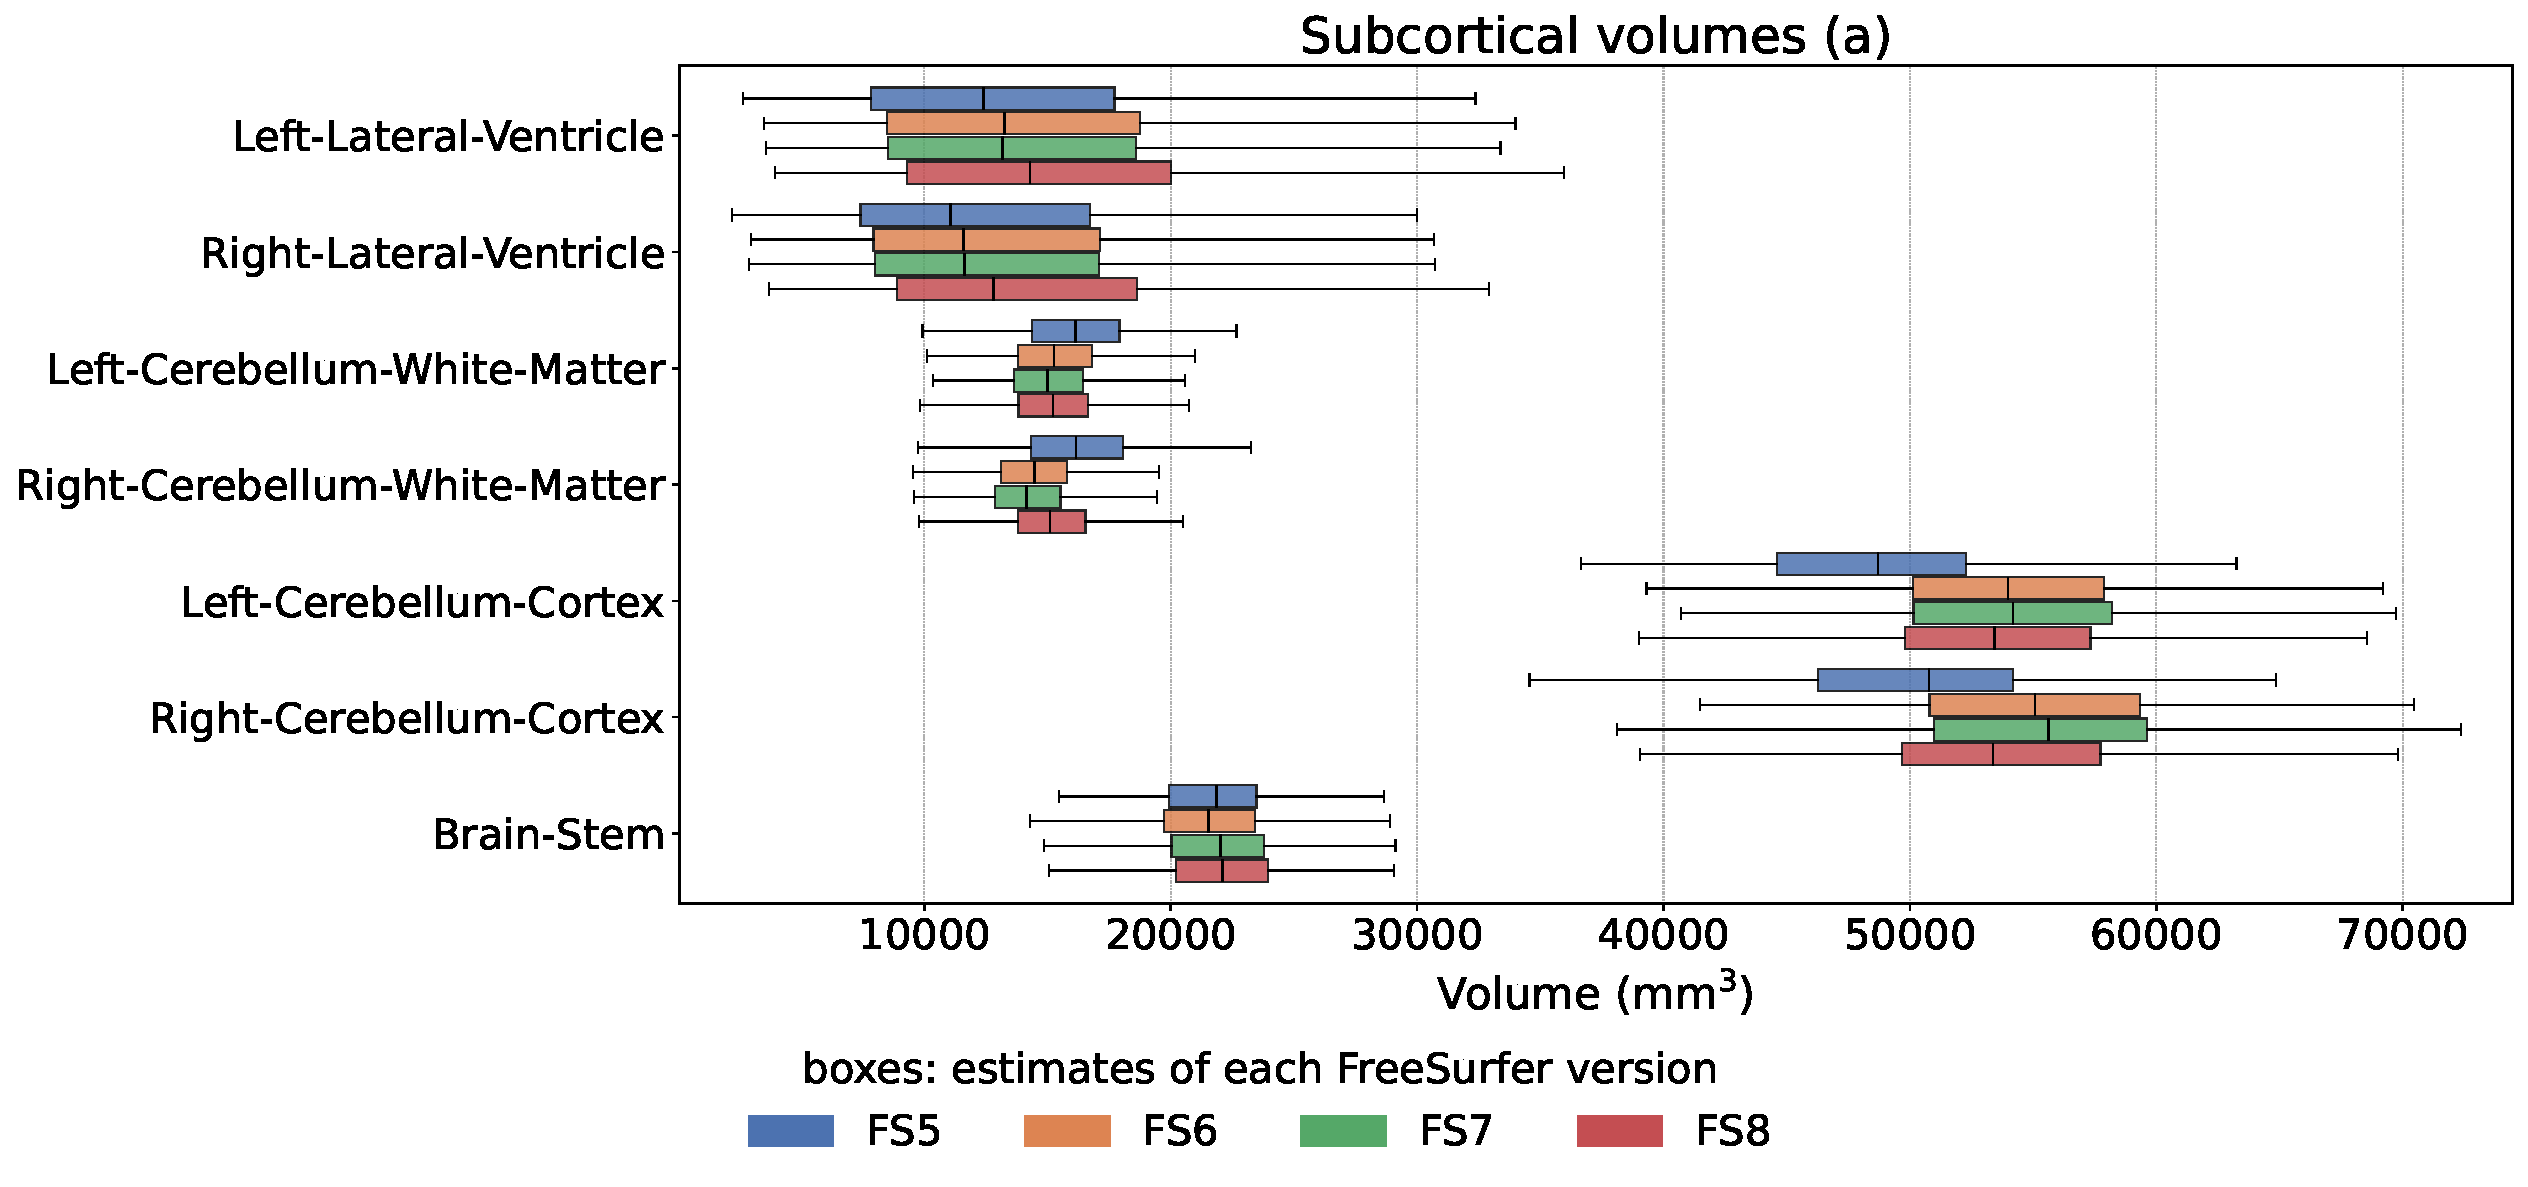
\includegraphics[width=\linewidth,height=0.85\textheight,keepaspectratio]{estimates_subcortical_part1}
\caption{Subcortical volume estimates per FreeSurfer version (830 images)\rev{, (a) lateral ventricles, cerebellum
(white matter and cortex) and brainstem, (b) other structures, on separate axes because their volumes are an order
of magnitude larger. The FS8 CSF volume is not shown: it includes the extracerebral CSF and is not comparable with
the other versions. Outliers beyond the x-axis range are not shown.}}
\end{figure}

\begin{figure}[p]
\ContinuedFloat
\centering
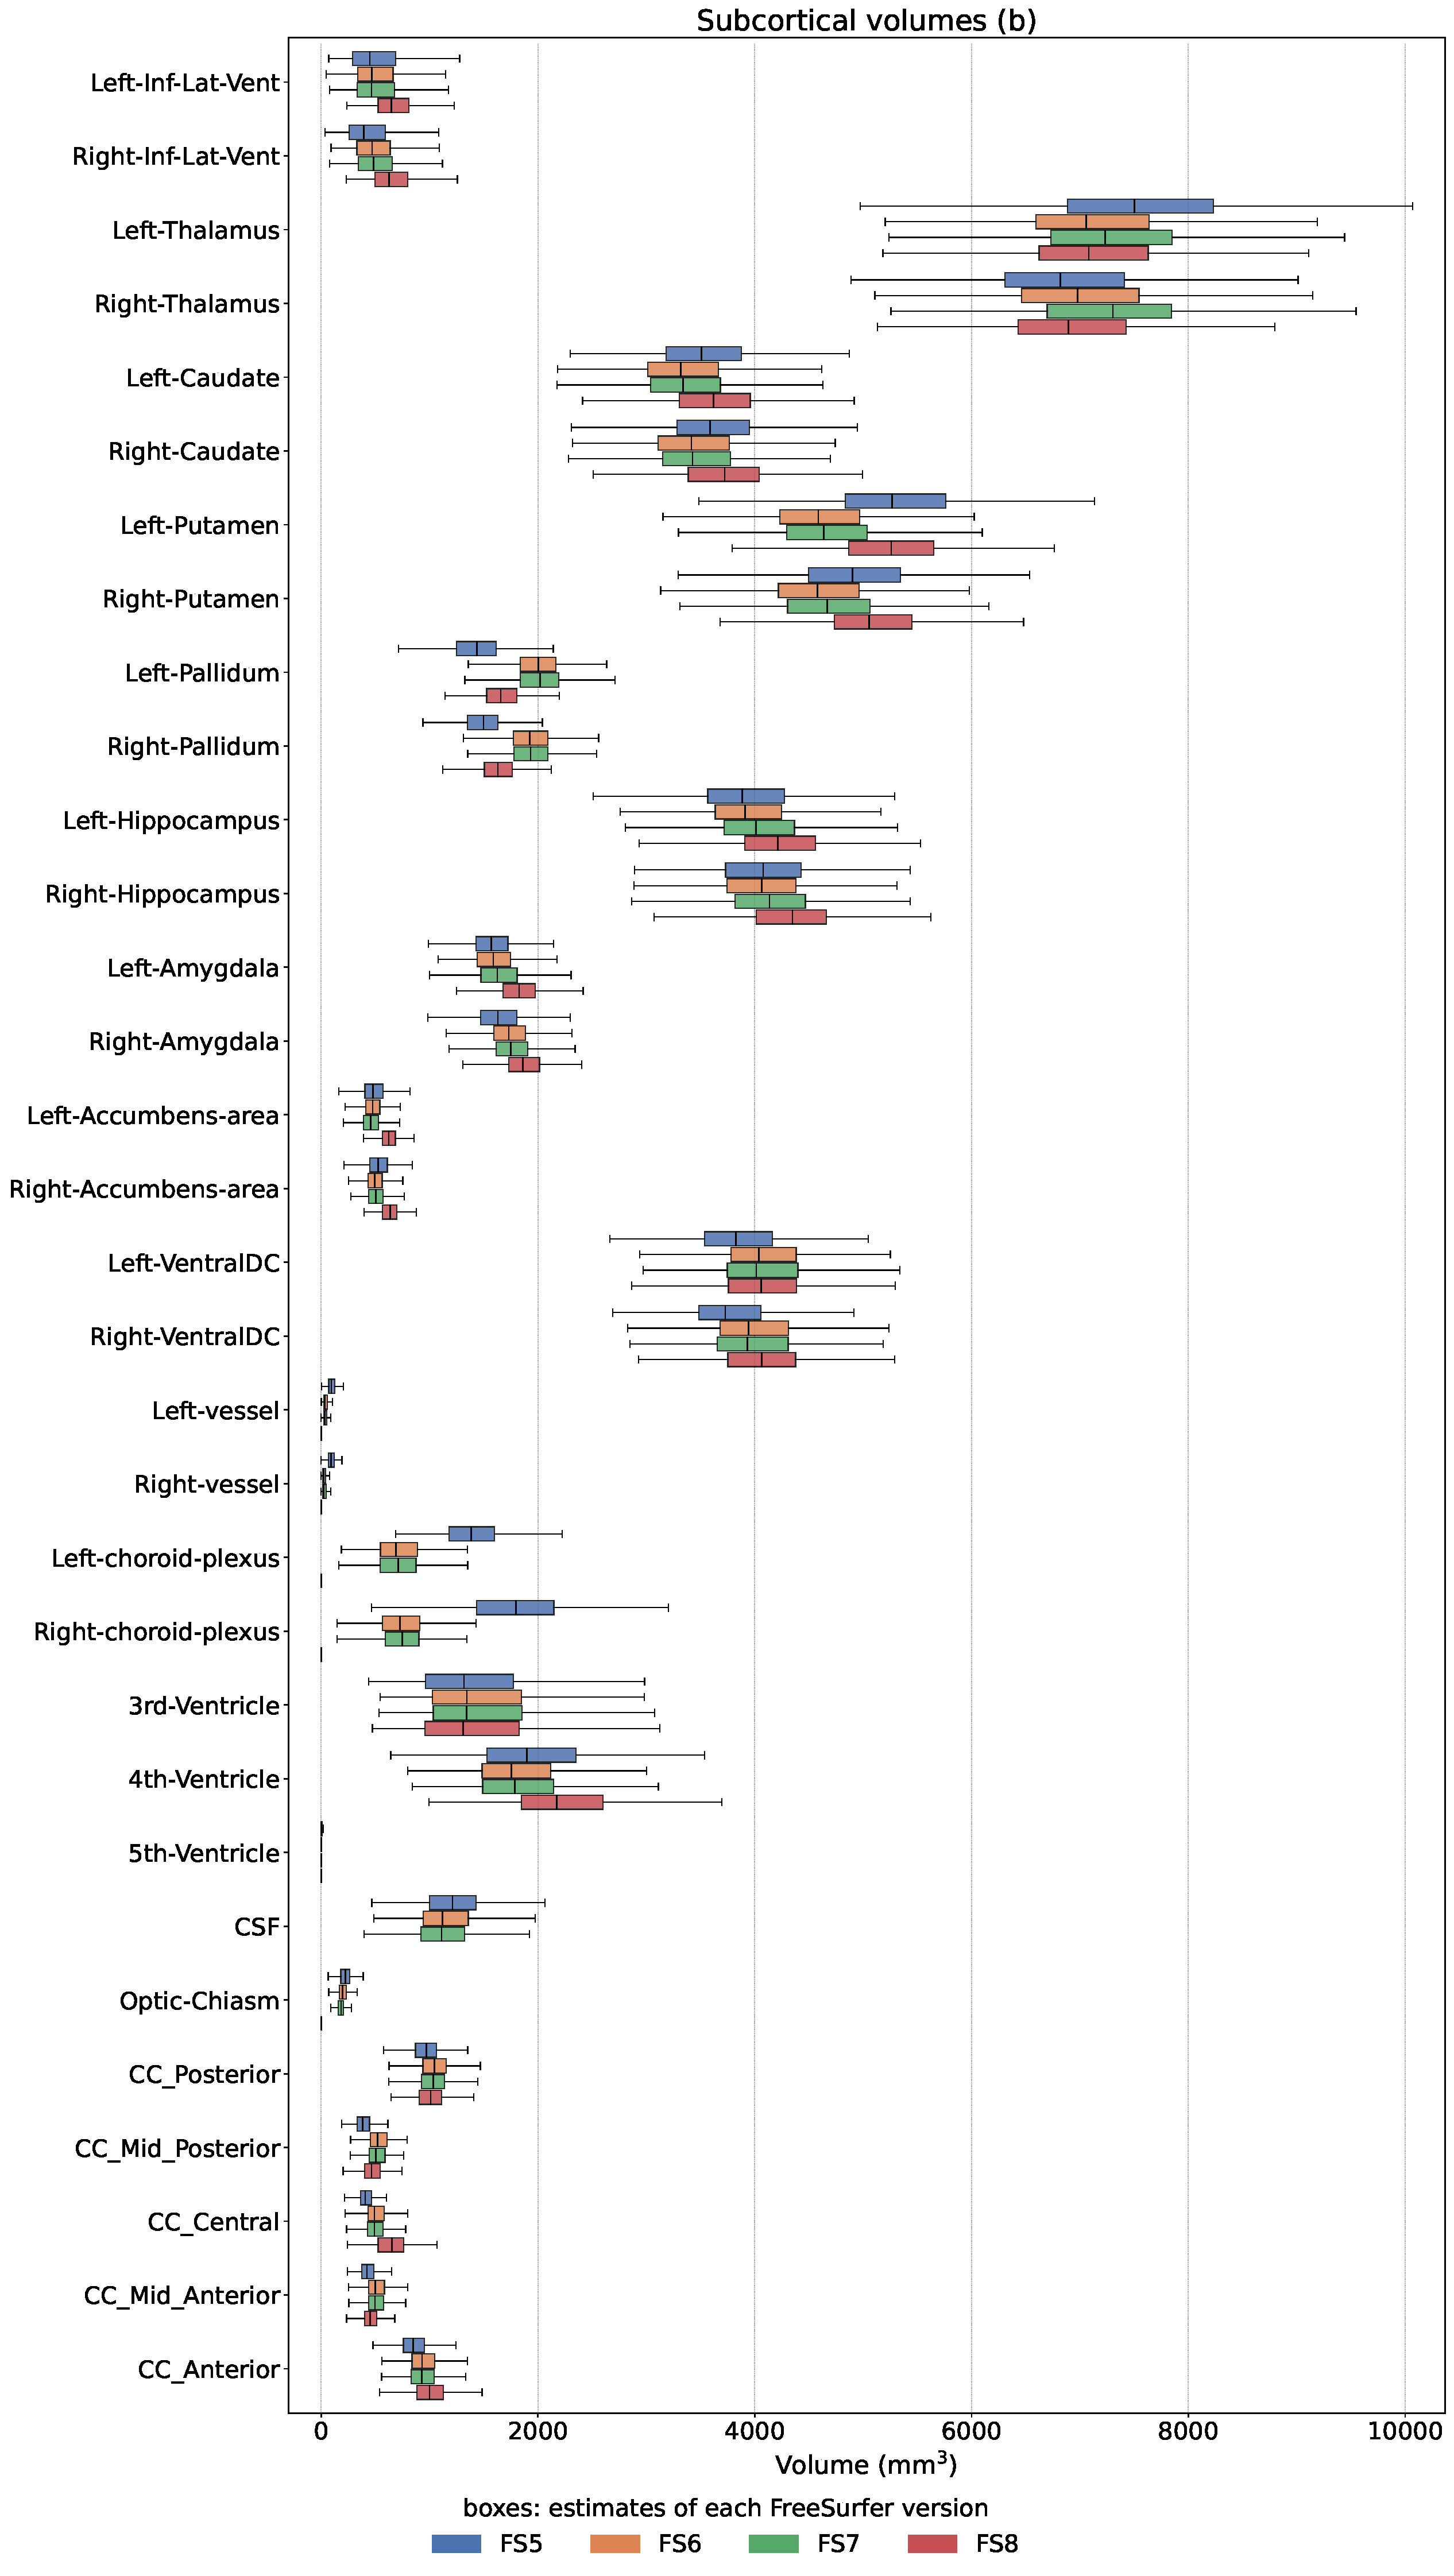
\includegraphics[width=\linewidth,height=0.85\textheight,keepaspectratio]{estimates_subcortical_part2}
\caption{\rev{(continued) (b) Other subcortical structures.}}
\end{figure}

\begin{figure}[p]
\centering
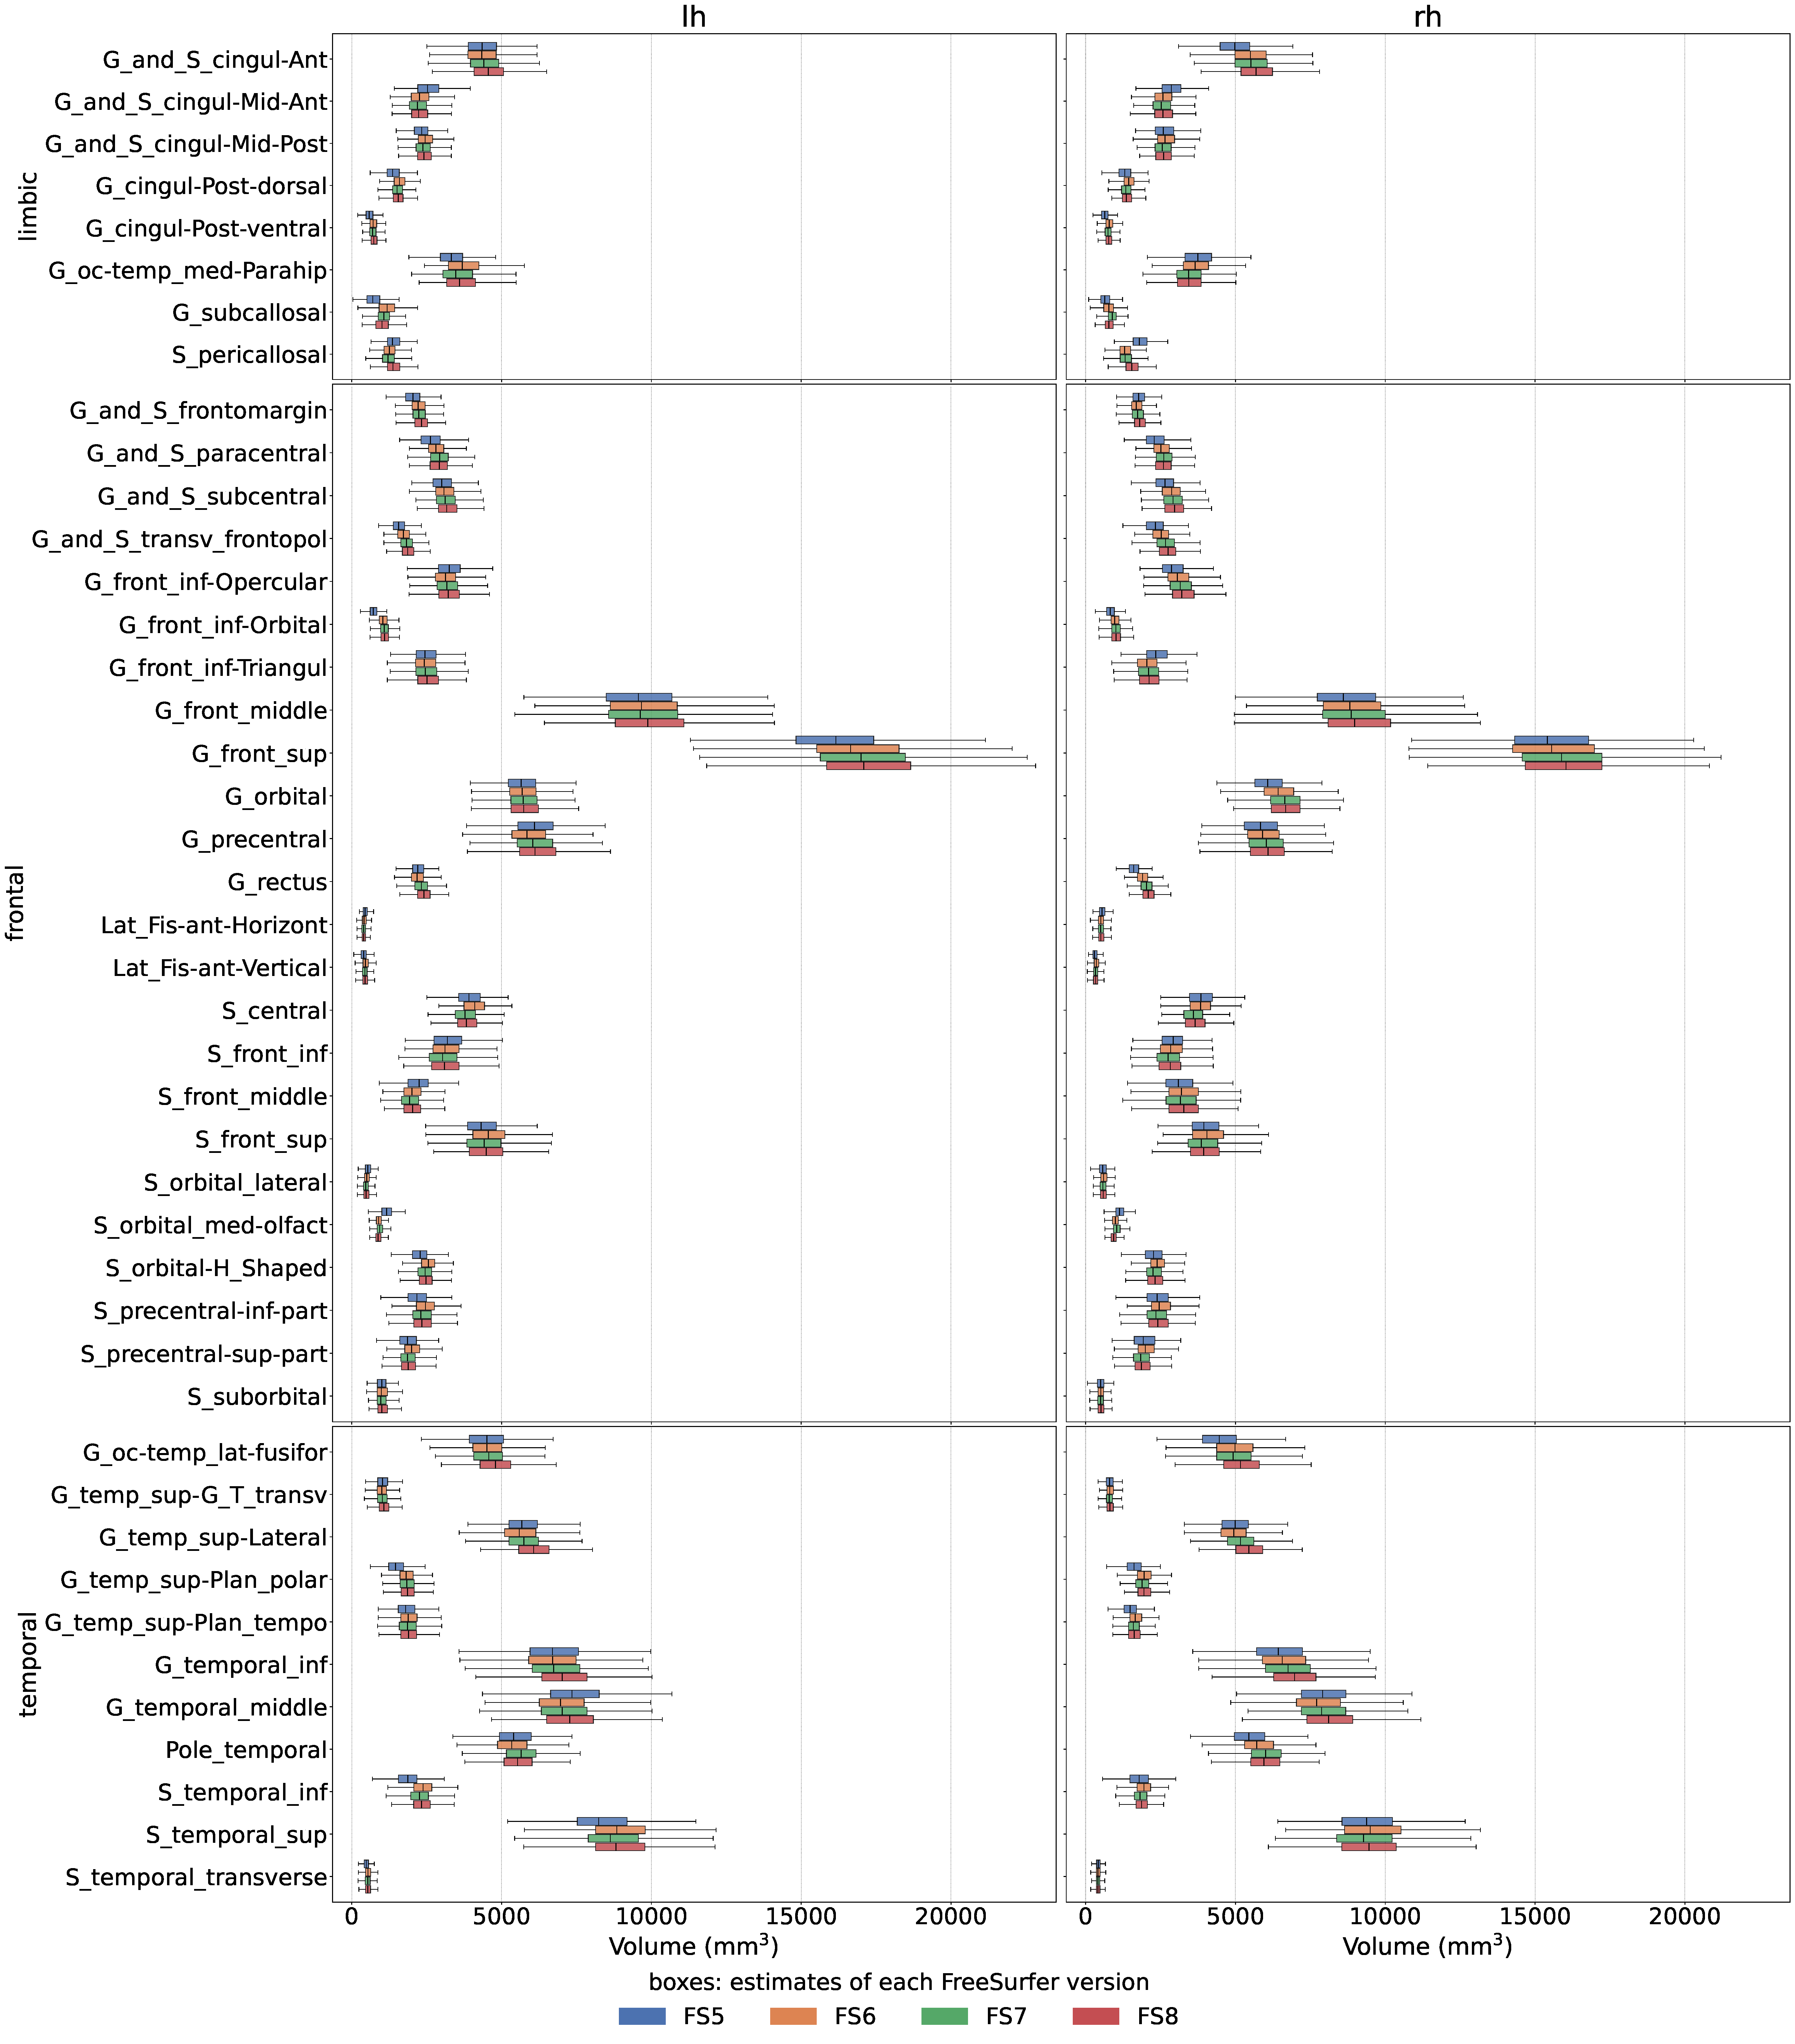
\includegraphics[width=\linewidth,height=0.85\textheight,keepaspectratio]{estimates_cortical_vol_part1}
\caption{Cortical volume, surface area and thickness estimates per FreeSurfer version (Destrieux atlas, 830
images)\rev{: (a) volume, (b) surface area, (c) cortical thickness, in the left (left panels) and right (right
panels) hemispheres, each in two parts: limbic, frontal and temporal regions, then occipital, parietal and other
regions. Outliers beyond the x-axis range are not shown.}}
\end{figure}

\begin{figure}[p]
\ContinuedFloat
\centering
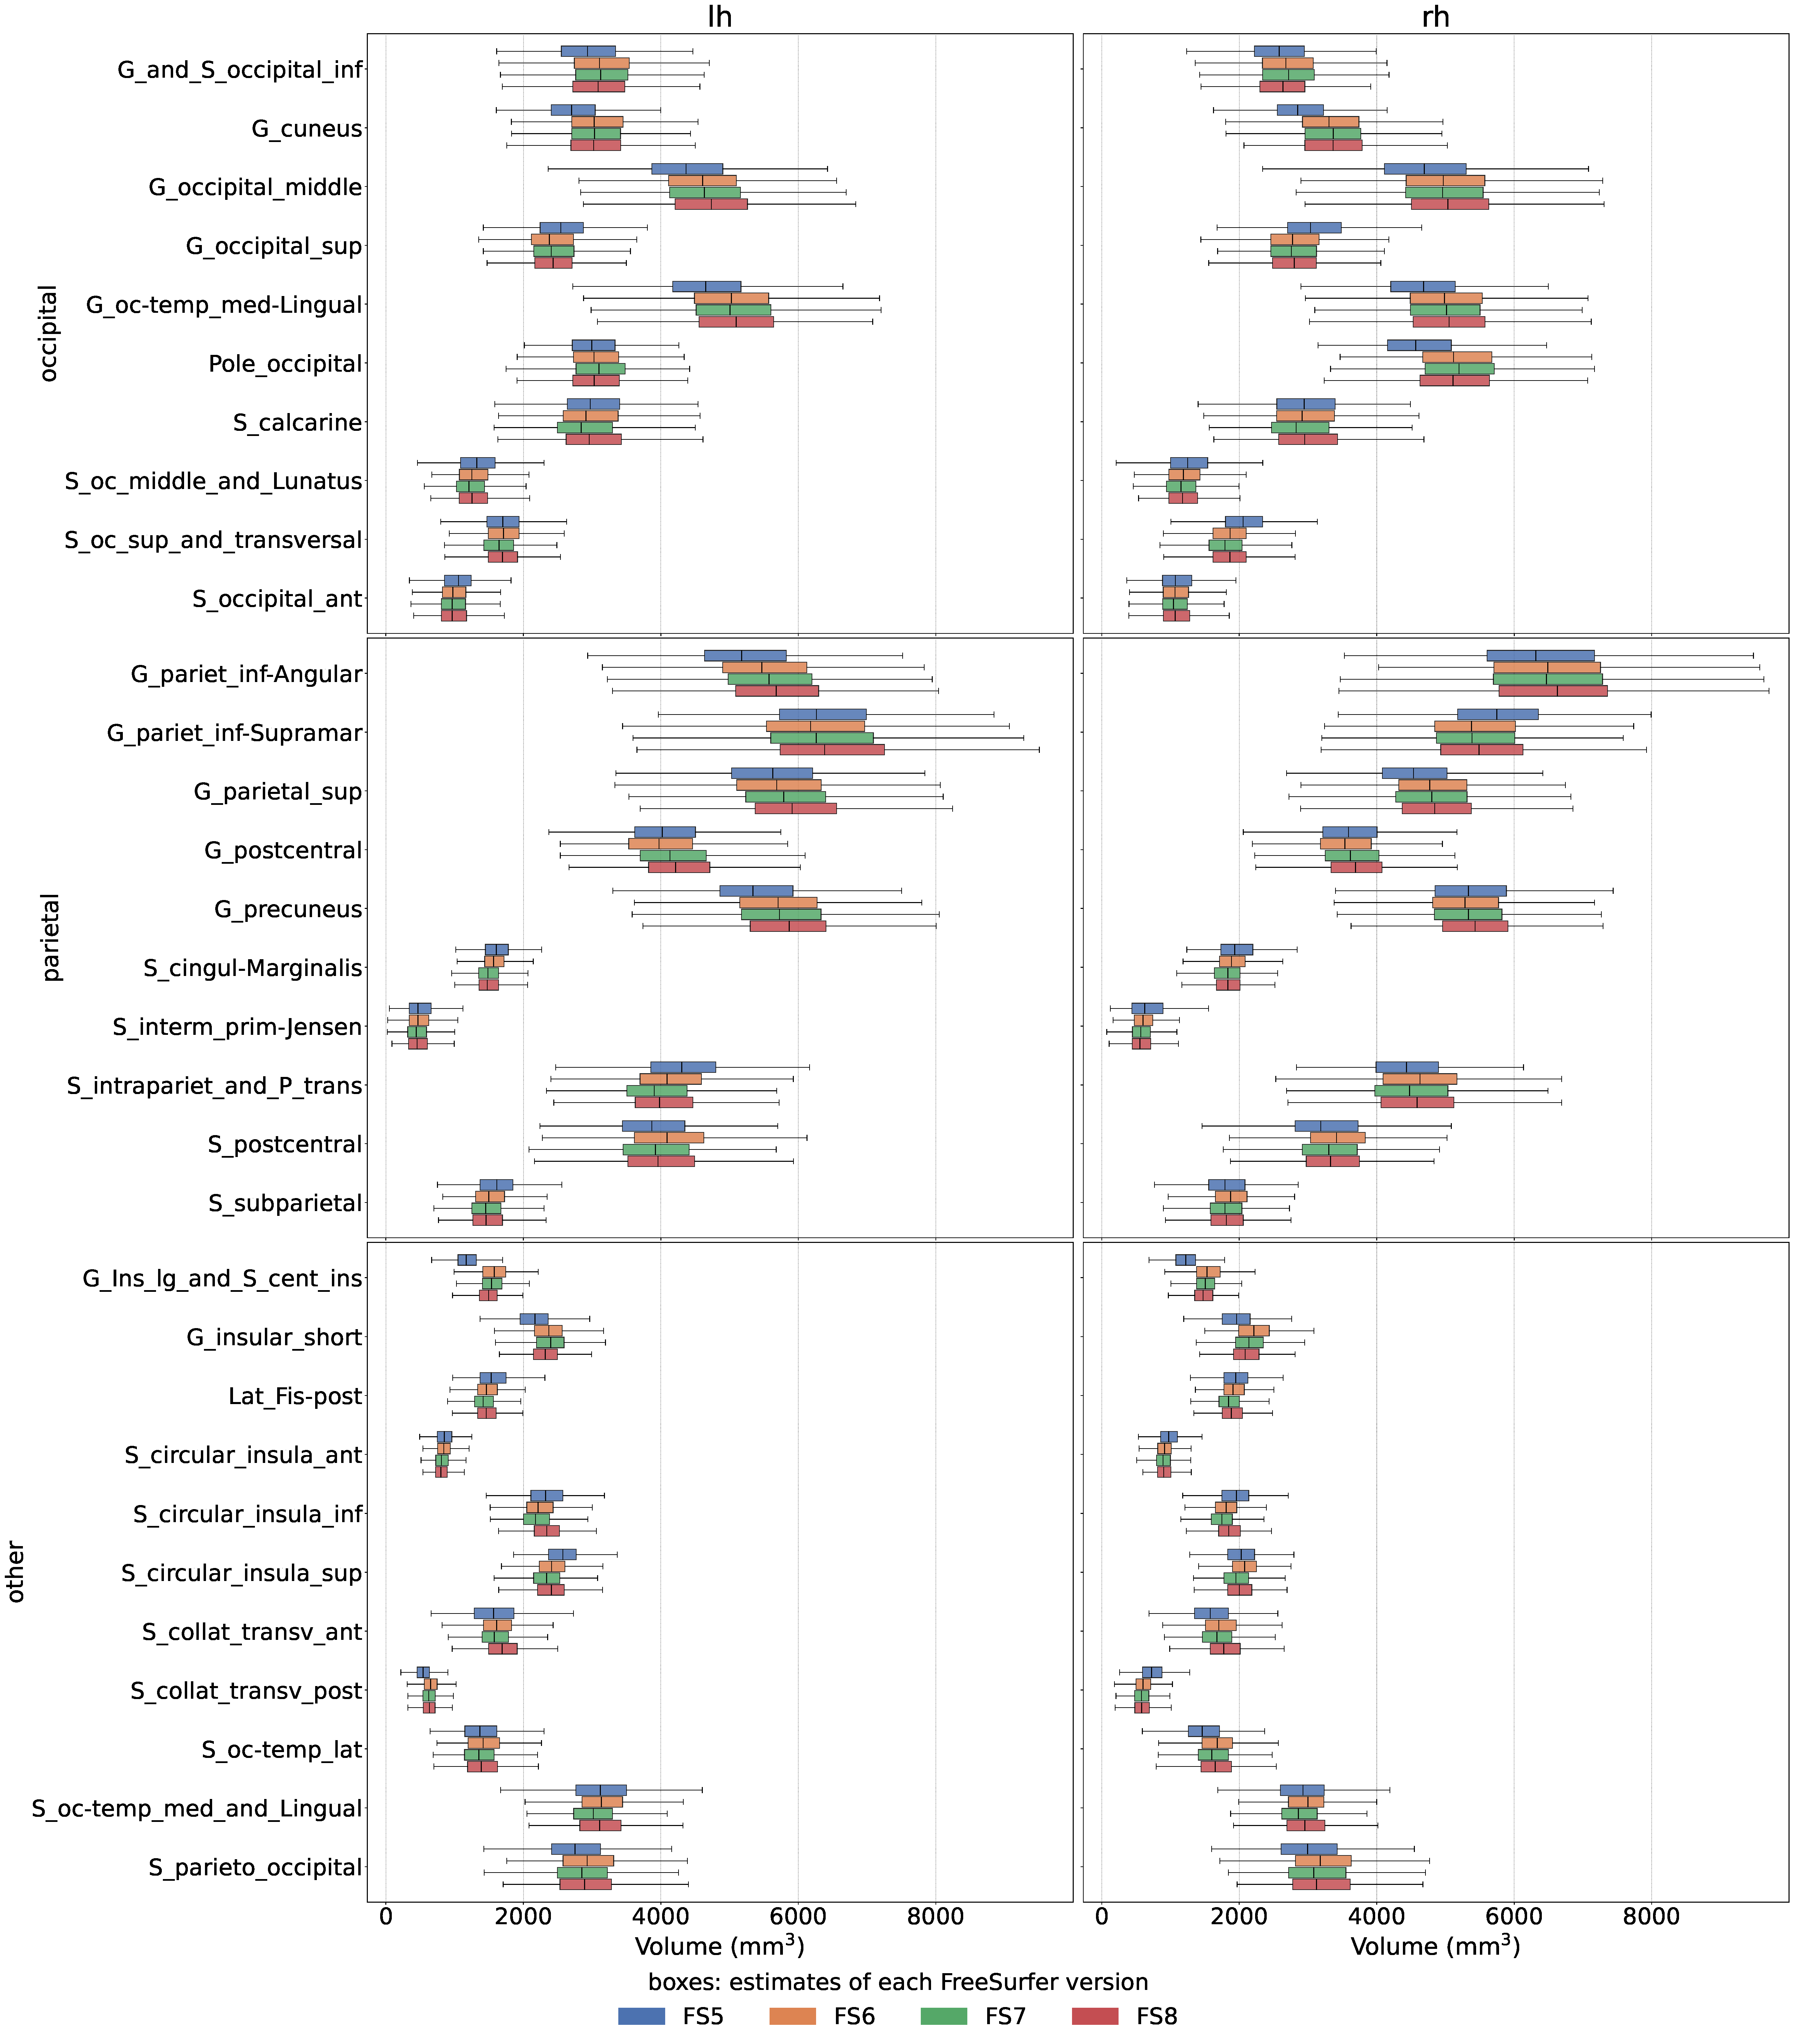
\includegraphics[width=\linewidth,height=0.85\textheight,keepaspectratio]{estimates_cortical_vol_part2}
\caption{\rev{(continued) (a) Volume: occipital, parietal and other regions.}}
\end{figure}

\begin{figure}[p]
\ContinuedFloat
\centering
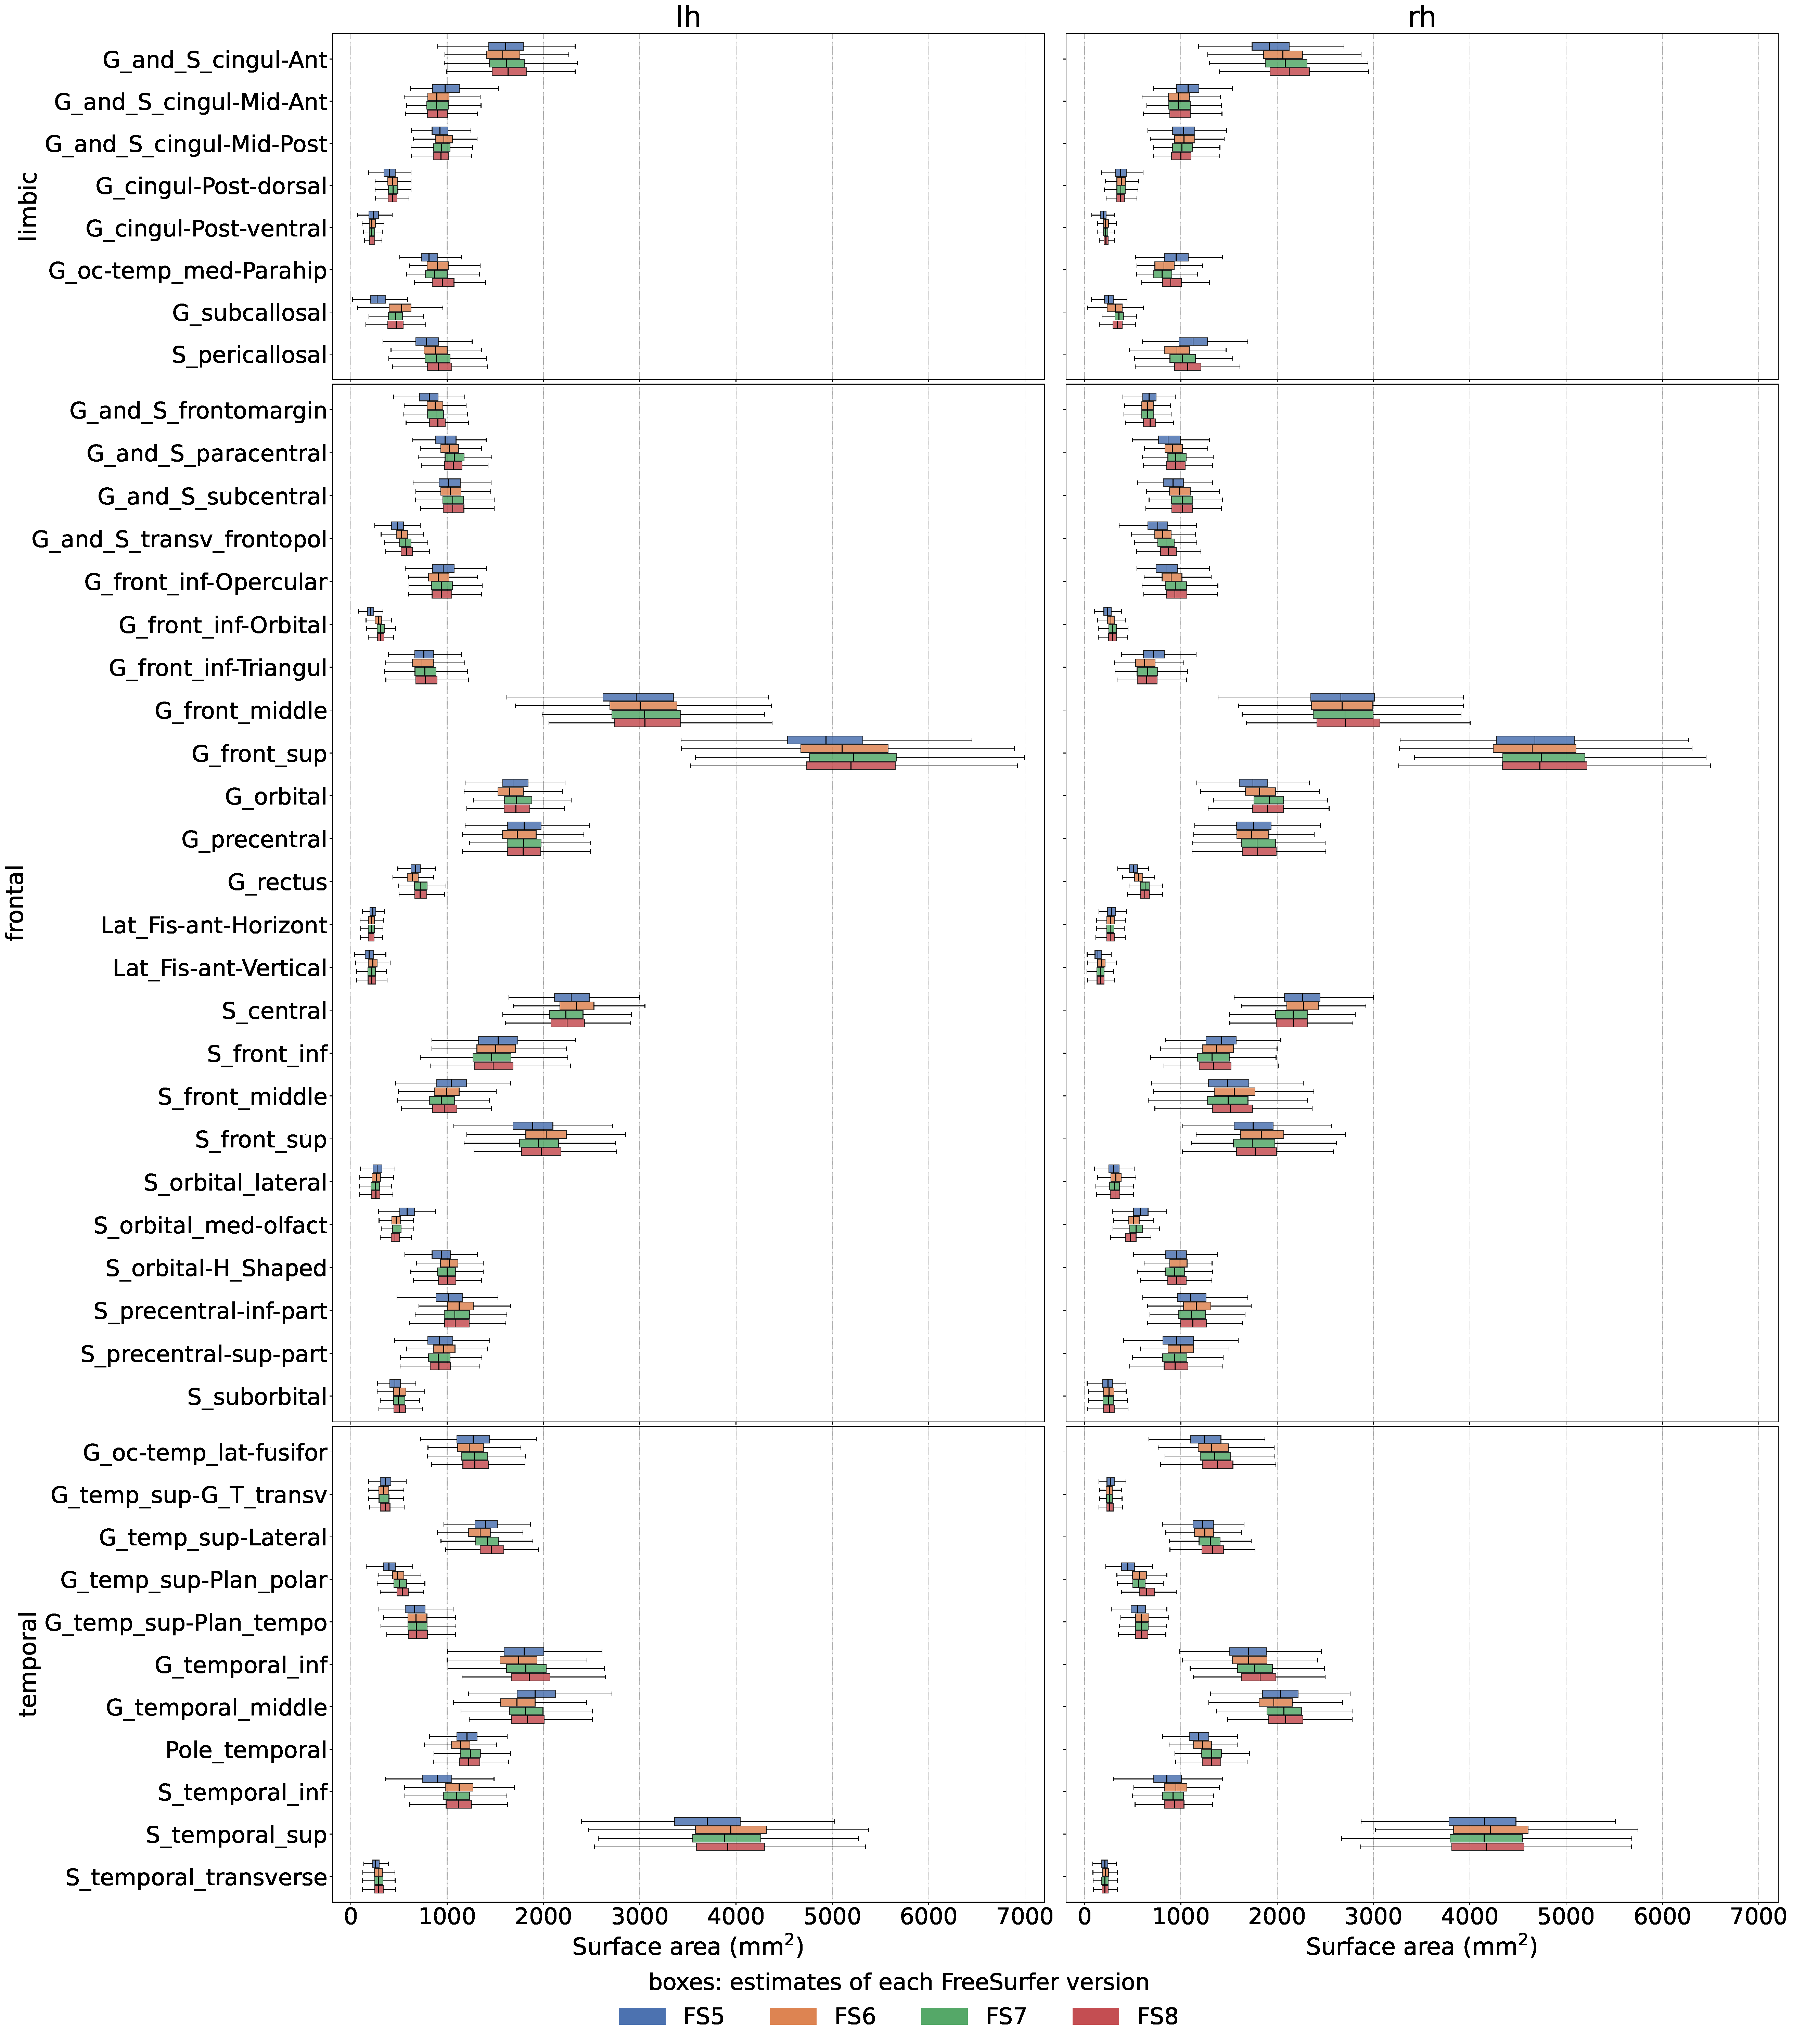
\includegraphics[width=\linewidth,height=0.85\textheight,keepaspectratio]{estimates_cortical_surf_part1}
\caption{\rev{(continued) (b) Surface area: limbic, frontal and temporal regions.}}
\end{figure}

\begin{figure}[p]
\ContinuedFloat
\centering
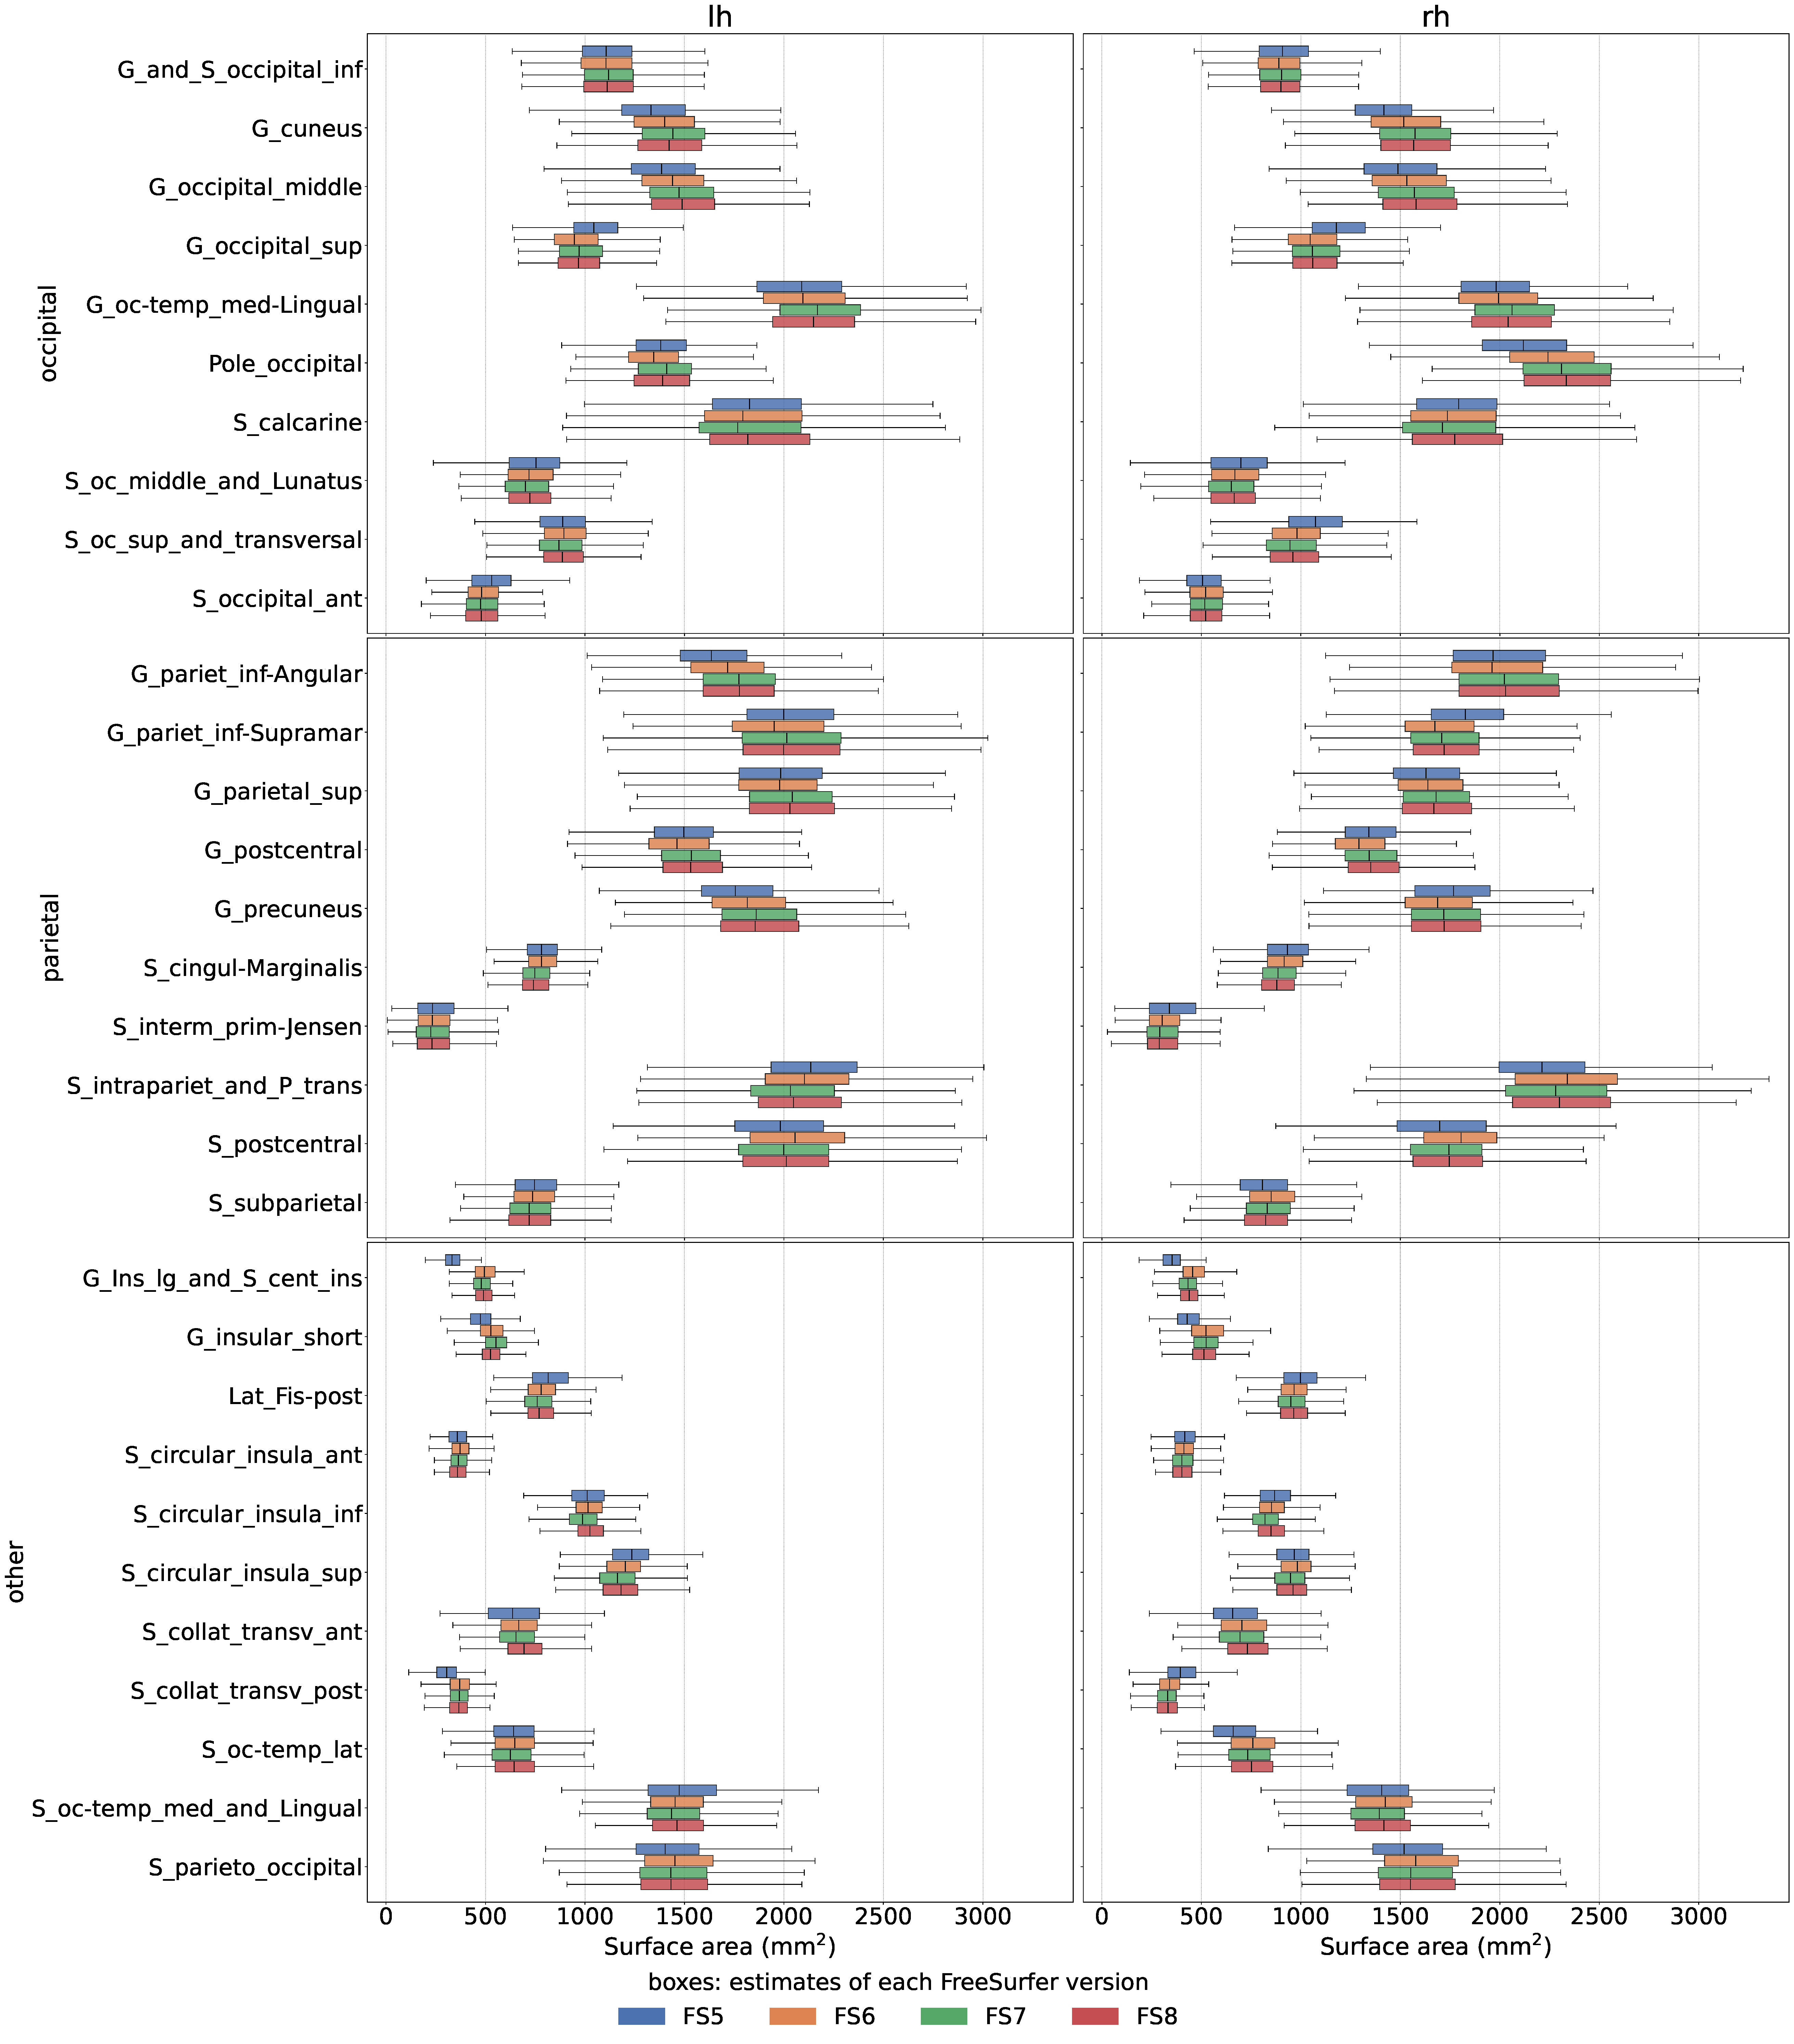
\includegraphics[width=\linewidth,height=0.85\textheight,keepaspectratio]{estimates_cortical_surf_part2}
\caption{\rev{(continued) (b) Surface area: occipital, parietal and other regions.}}
\end{figure}

\begin{figure}[p]
\ContinuedFloat
\centering
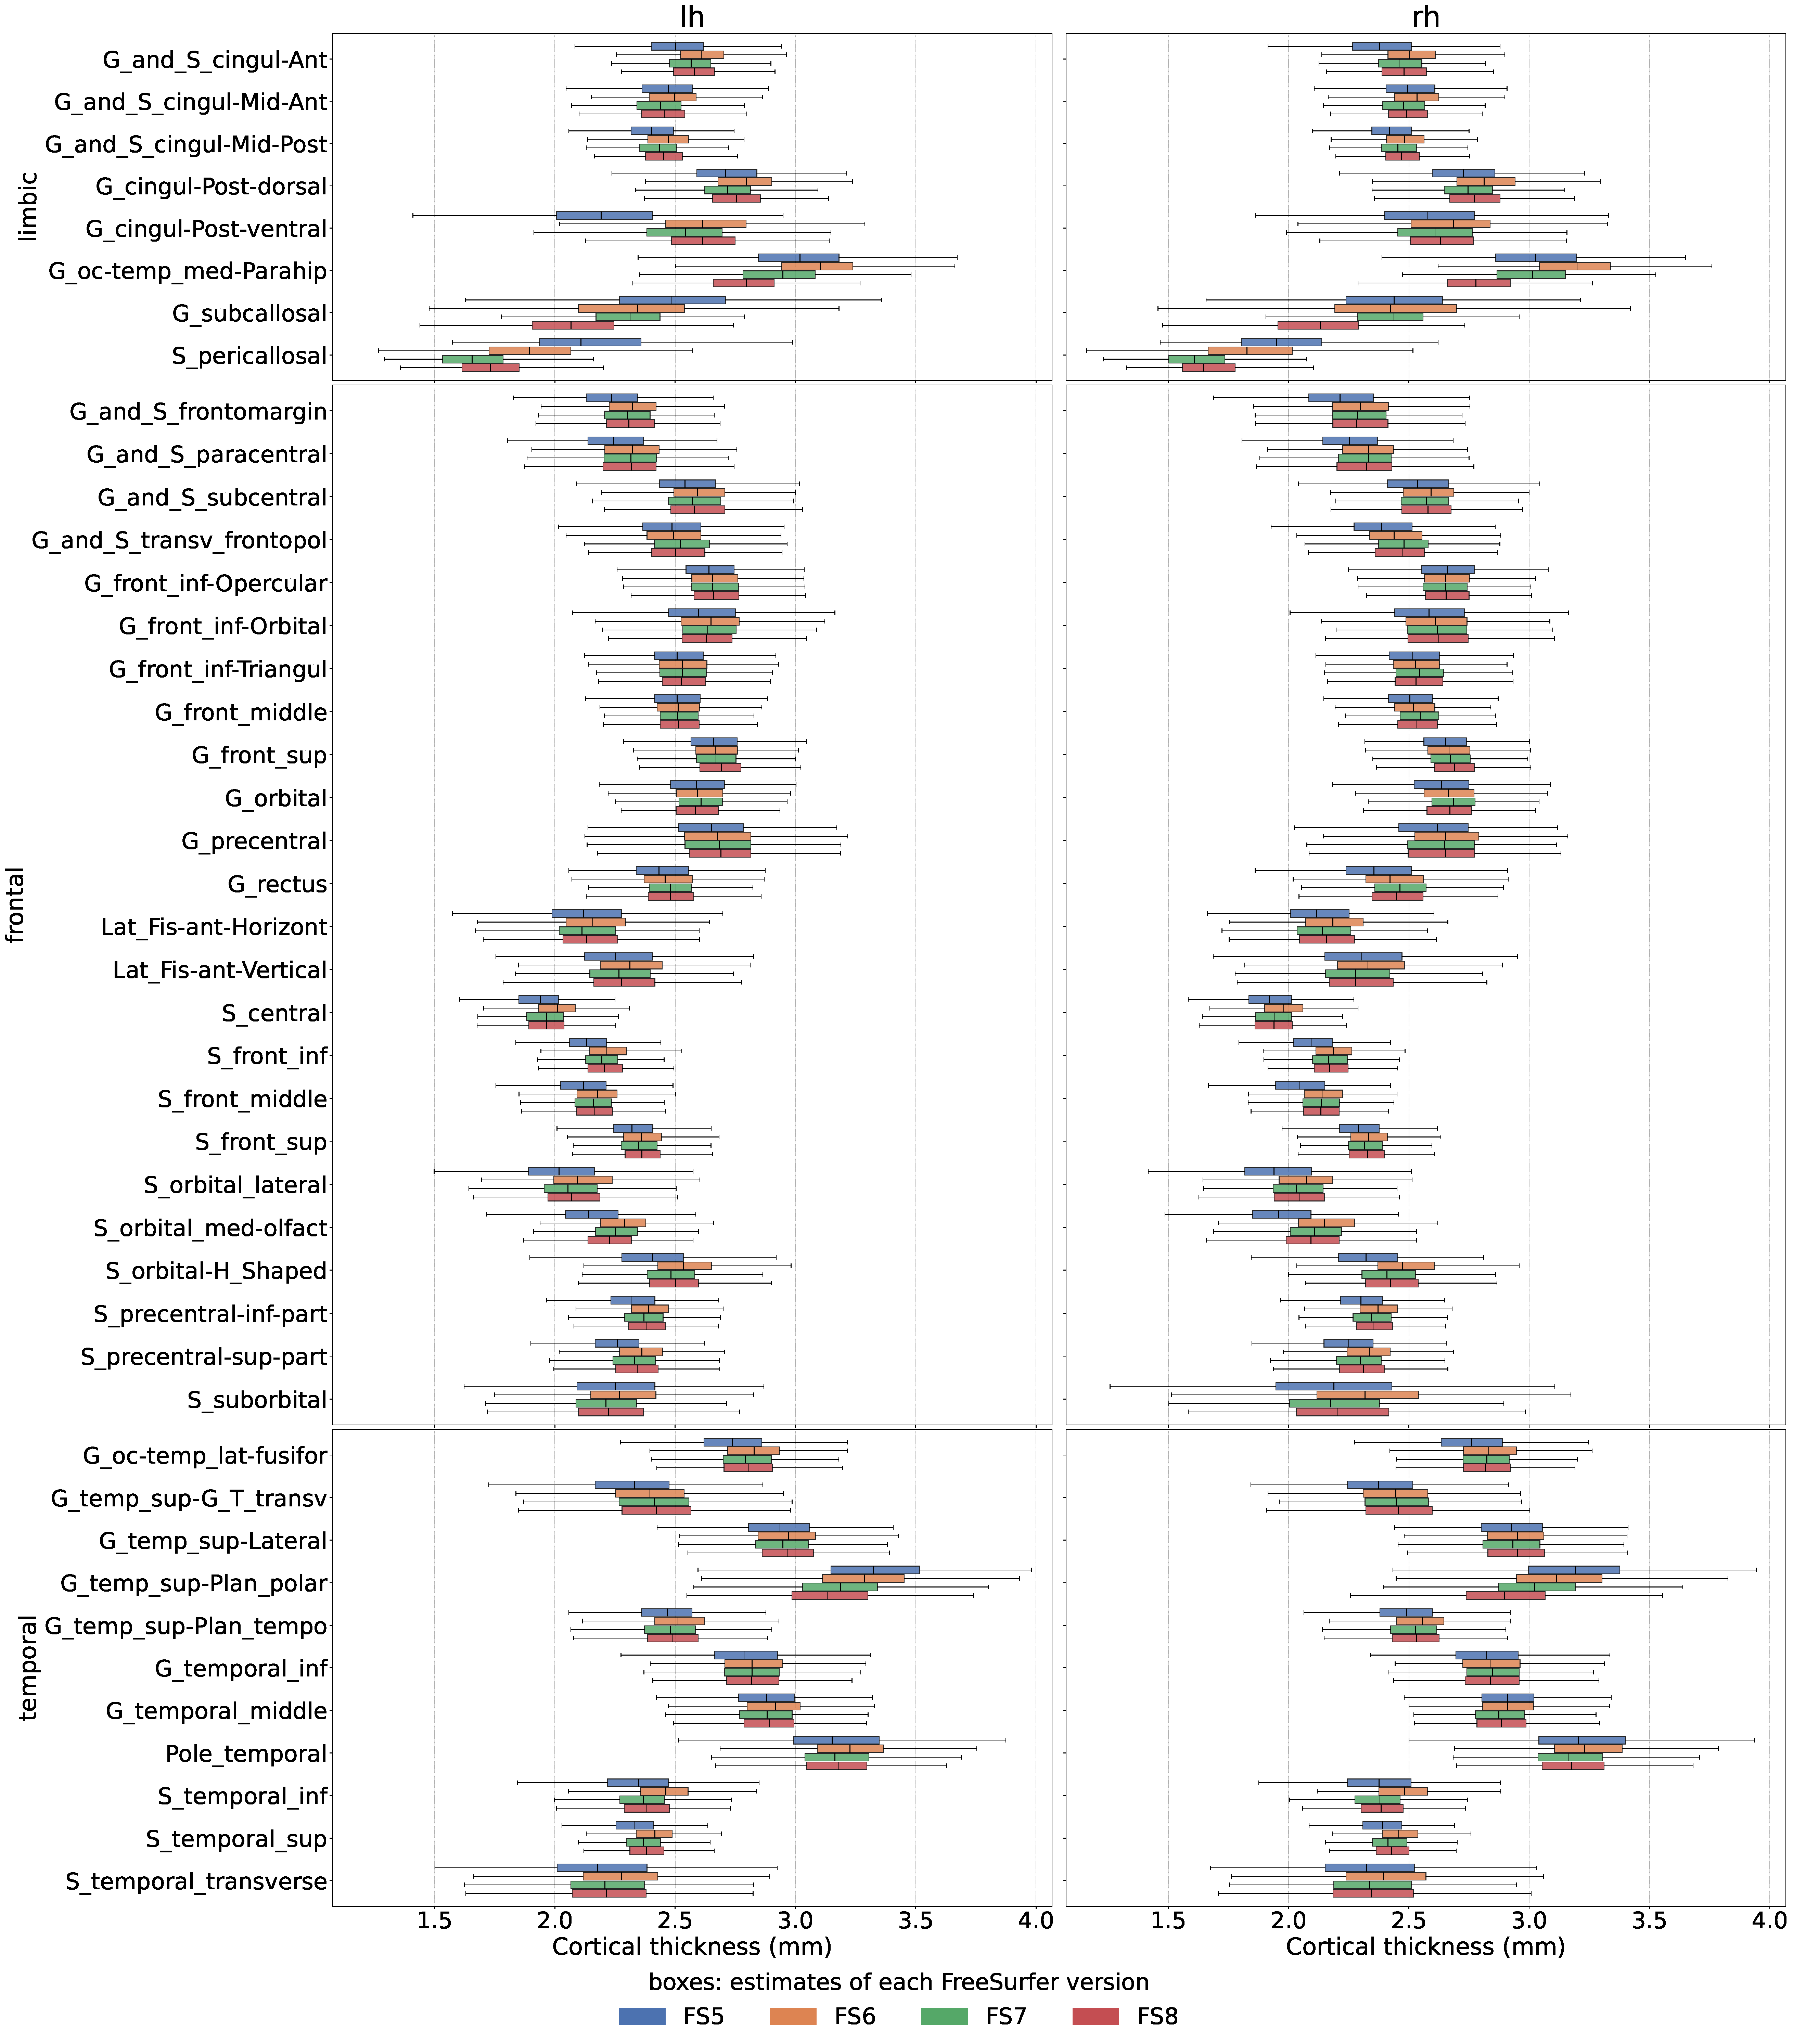
\includegraphics[width=\linewidth,height=0.85\textheight,keepaspectratio]{estimates_cortical_ct_part1}
\caption{\rev{(continued) (c) Cortical thickness: limbic, frontal and temporal regions.}}
\end{figure}

\begin{figure}[p]
\ContinuedFloat
\centering
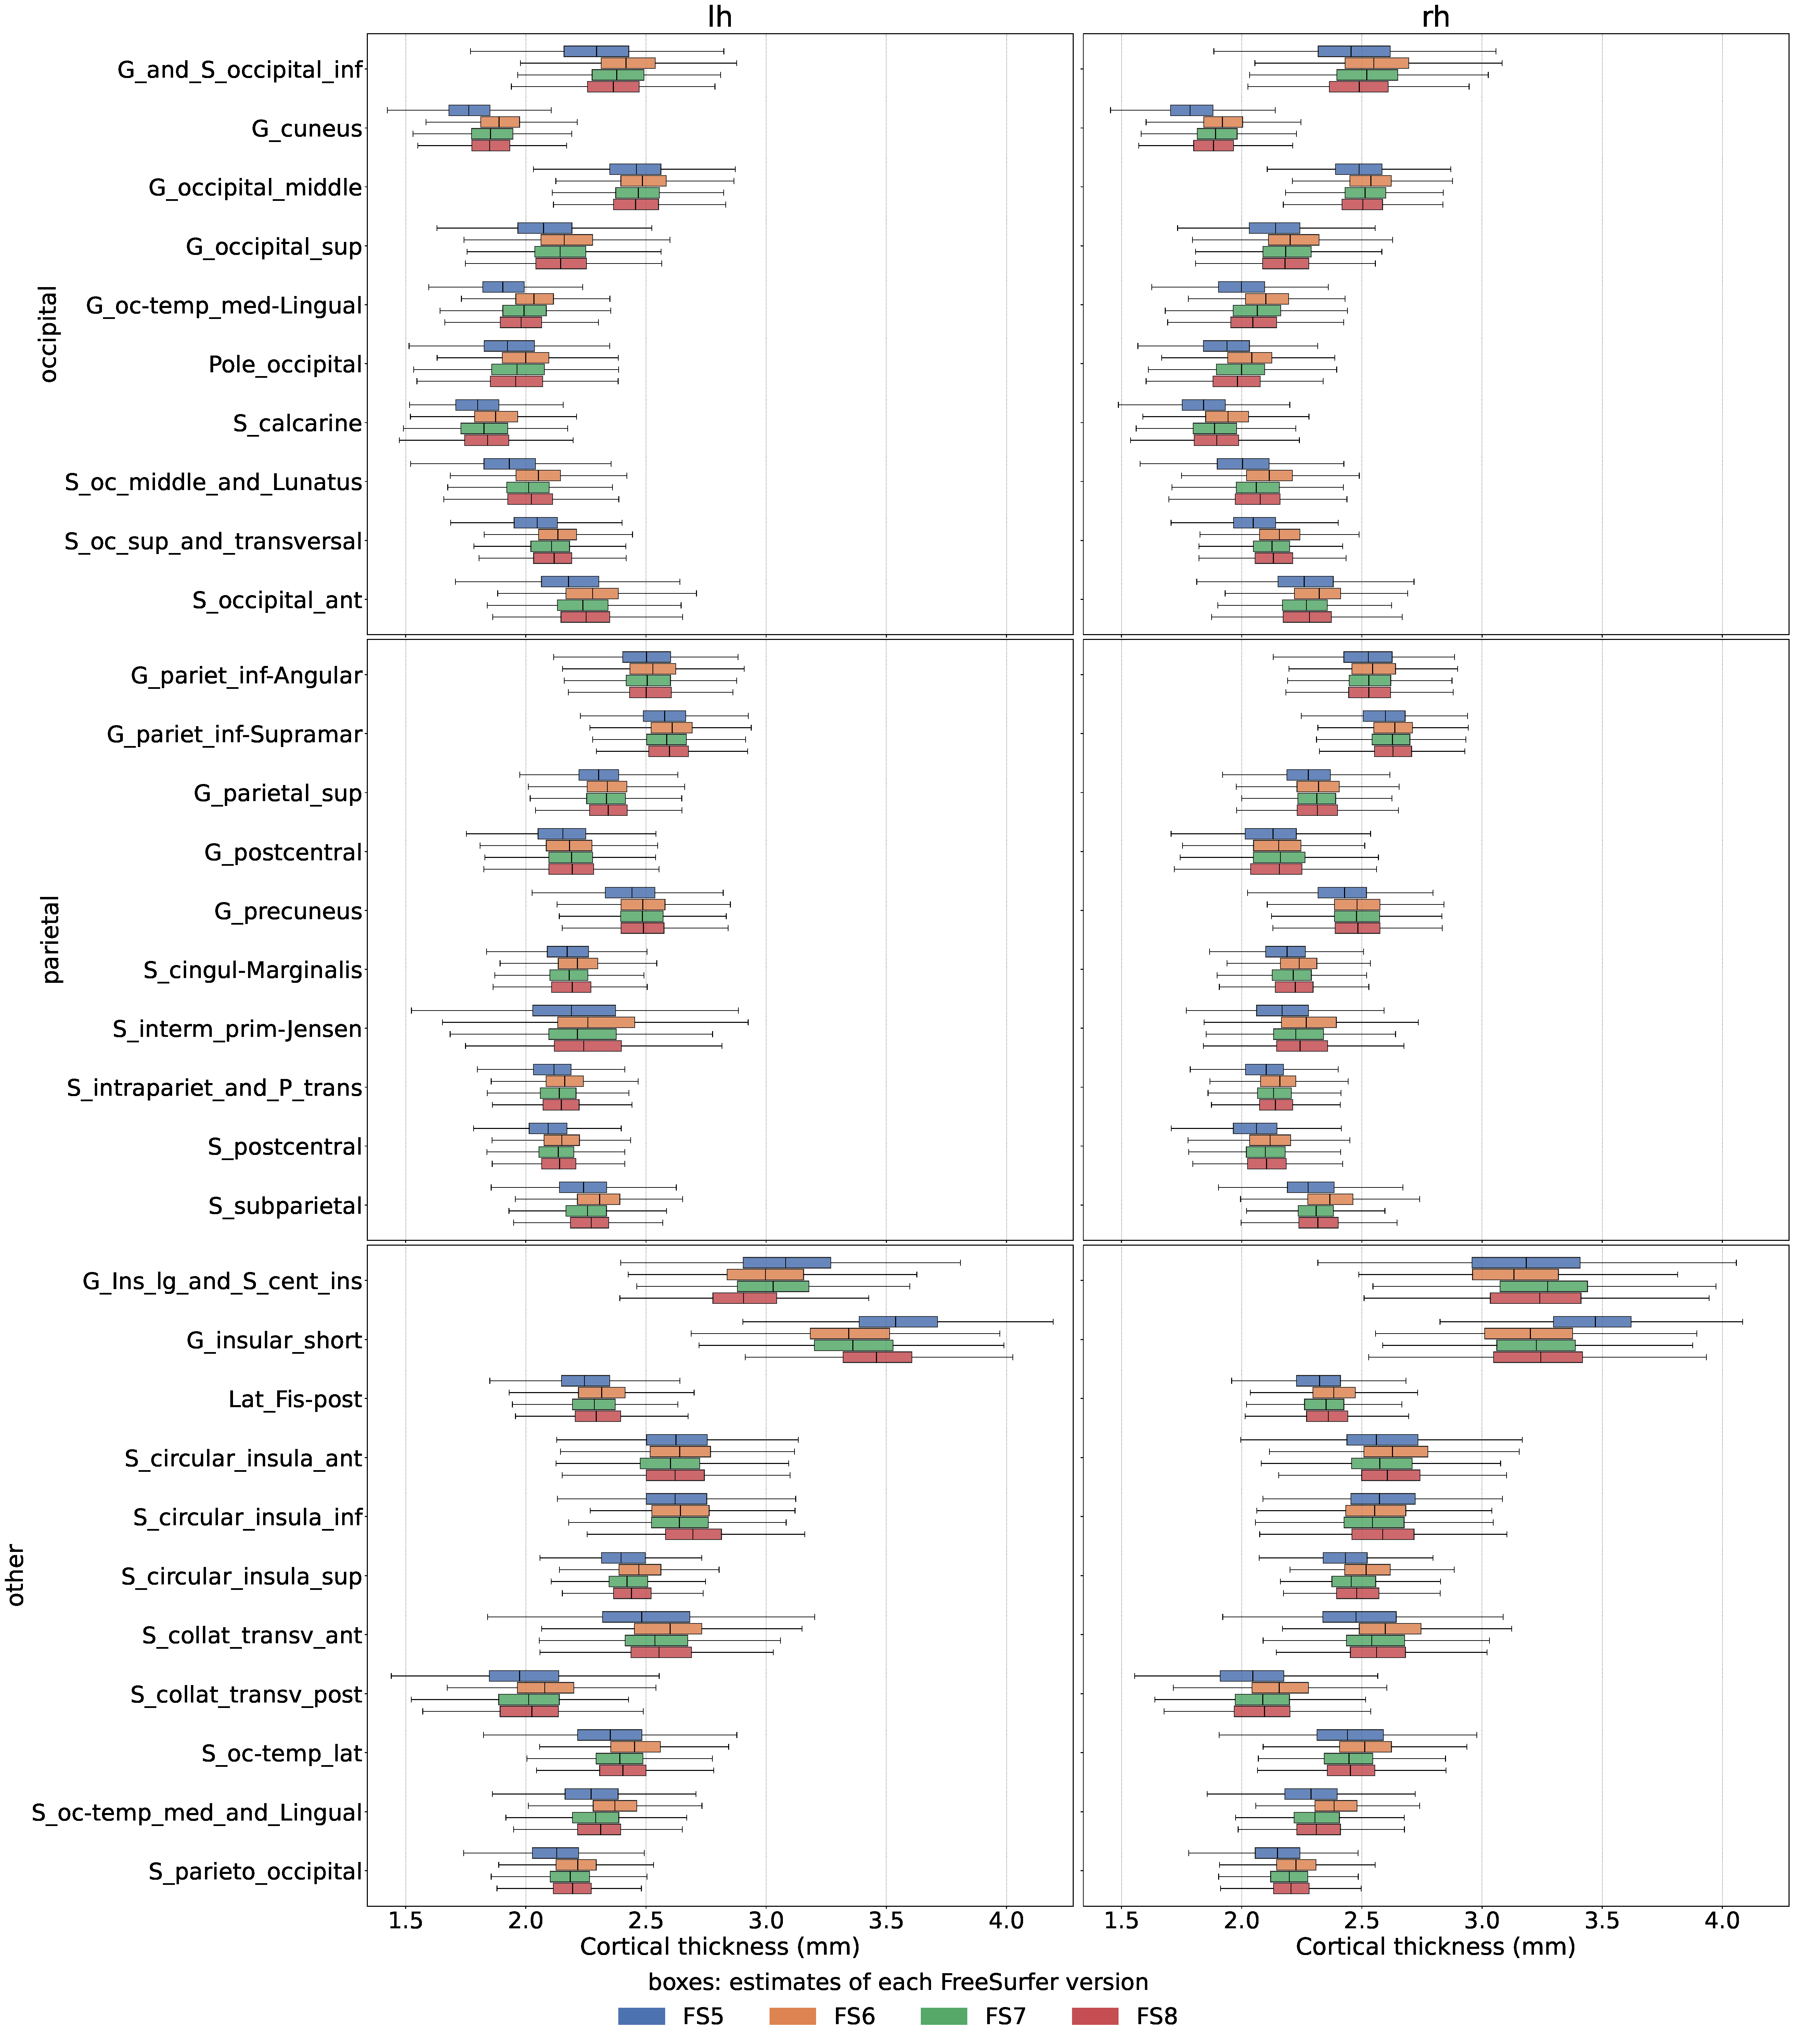
\includegraphics[width=\linewidth,height=0.85\textheight,keepaspectratio]{estimates_cortical_ct_part2}
\caption{\rev{(continued) (c) Cortical thickness: occipital, parietal and other regions.}}
\end{figure}

\begin{figure}[p]
\centering
\includegraphics[width=\linewidth]{hippocampi_example}
\caption{Hippocampus segmentations. \note{Legend from the submitted Figure S5 to add; the figure shows FS5--7 and
was not regenerated.}}
\end{figure}

\begin{figure}[p]
\centering
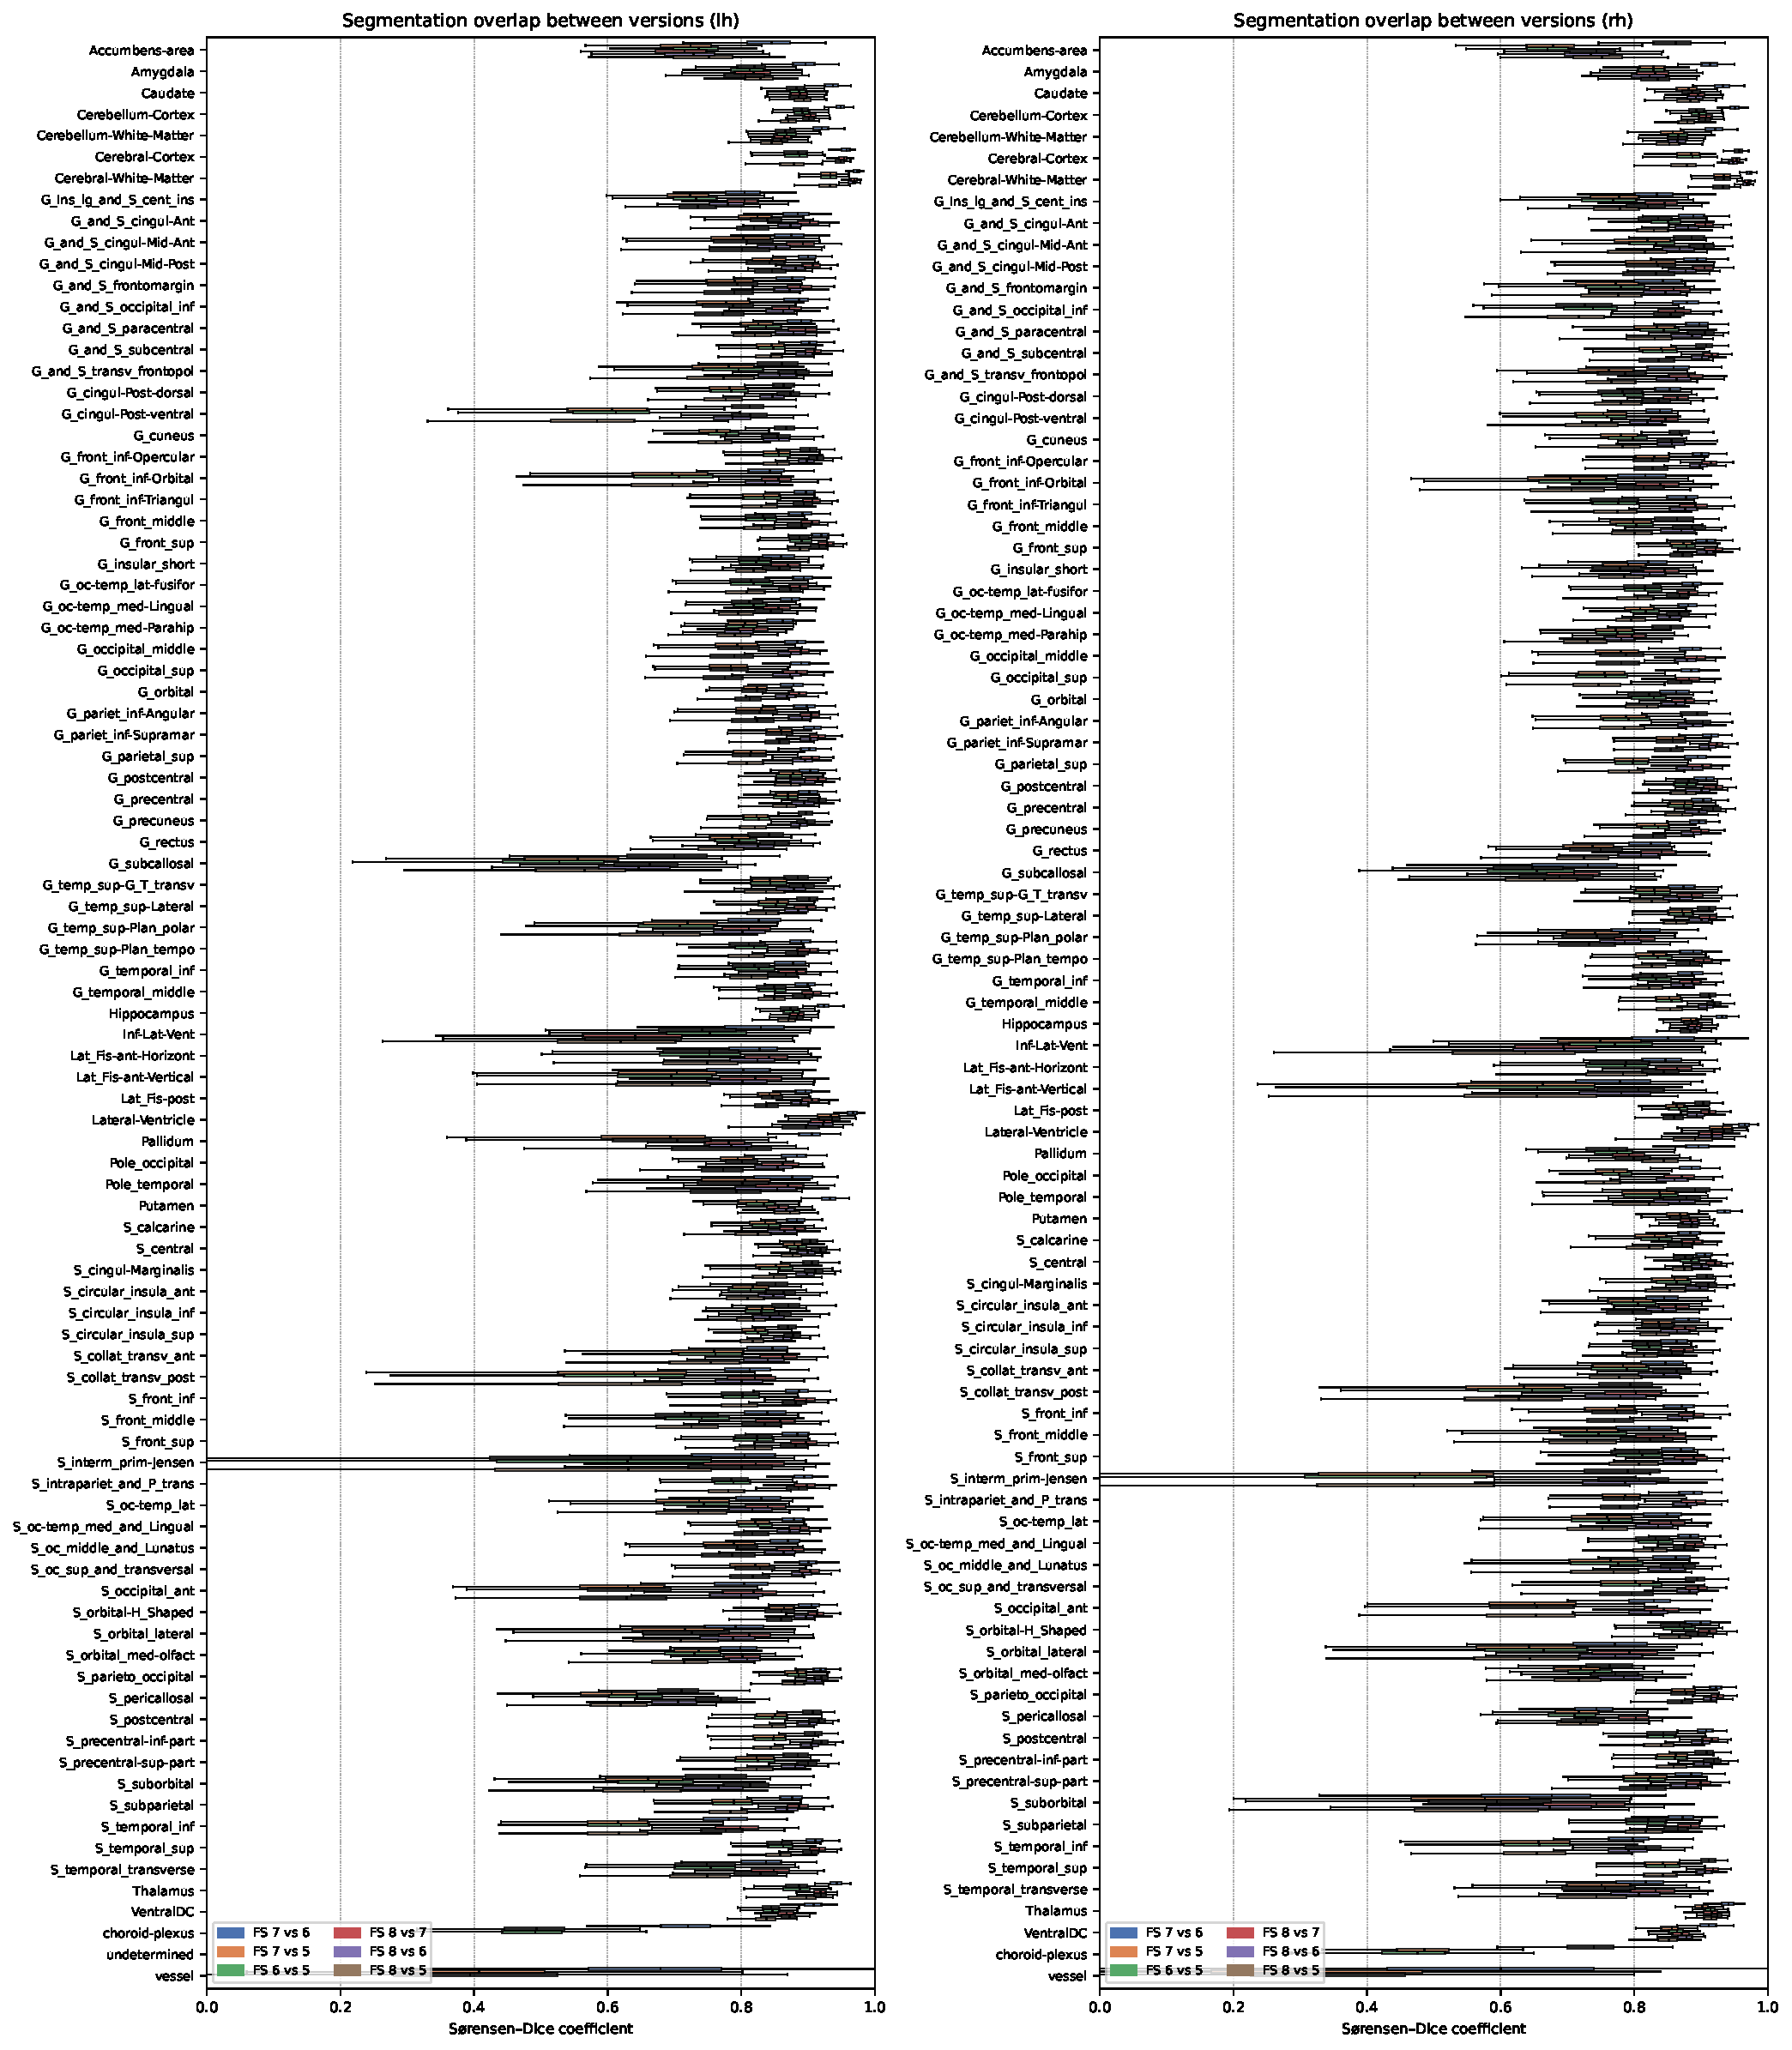
\includegraphics[width=\linewidth,height=0.85\textheight,keepaspectratio]{segmentation_dice}
\caption{Segmentation overlap between FreeSurfer versions: Sørensen--Dice coefficient of each label
(\texttt{mri\_seg\_overlap}, aseg and Destrieux parcellation), per version pair.}
\end{figure}

\begin{figure}[p]
\centering
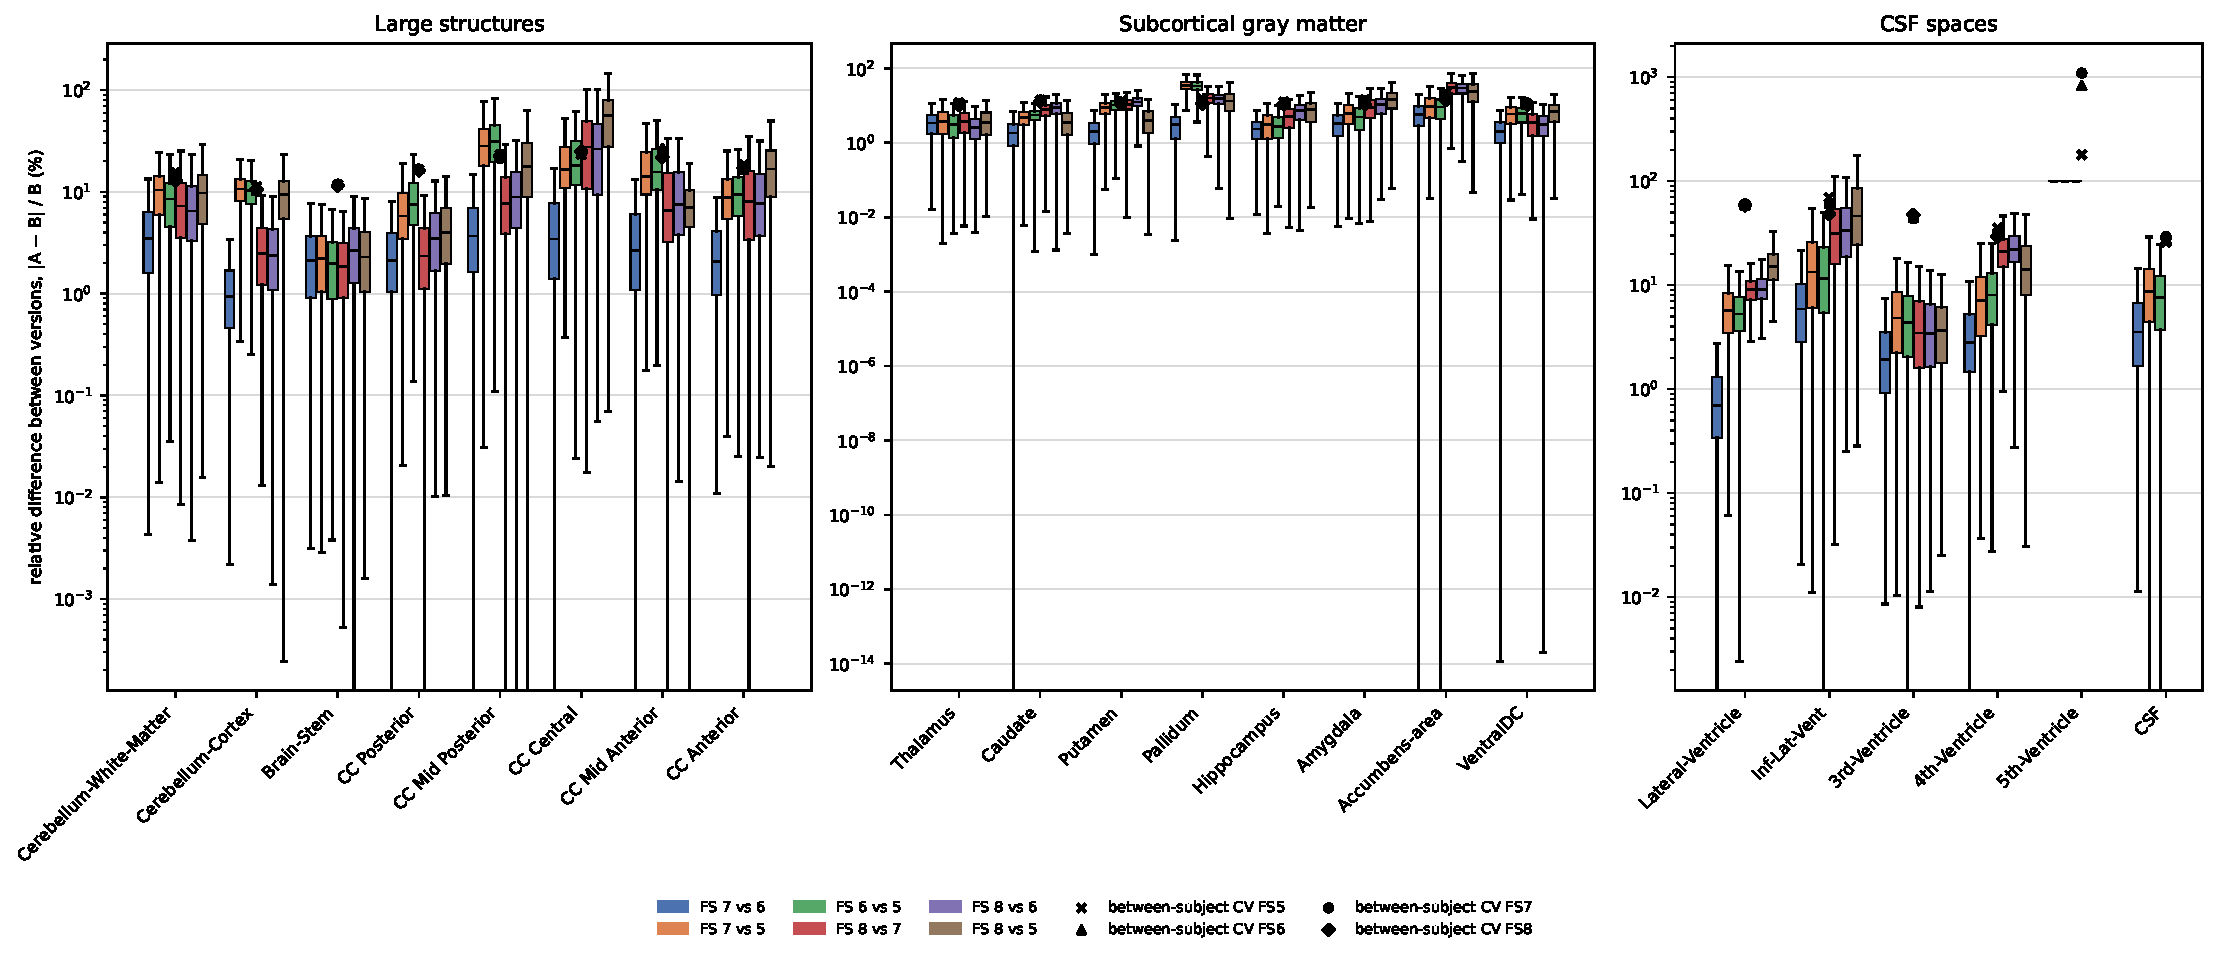
\includegraphics[width=\linewidth,height=0.8\textheight,keepaspectratio]{variability_by_type_subcortical}
\caption{\rev{Relative differences between FreeSurfer versions in subcortical volumes, by structure type (830
images; left and right merged: bilateral volume = left + right). Boxes: $|A - B|/B$ in \% for each version pair
(log scale); black markers: between-subject coefficient of variation (SD/mean, \%) of each version. Labels that FS8
does not produce (vessel, choroid plexus, optic chiasm, 5th ventricle) or defines differently (CSF, which in FS8
includes the extracerebral CSF) are left out of the FS8 pairs.}}
\end{figure}

\begin{figure}[p]
\centering
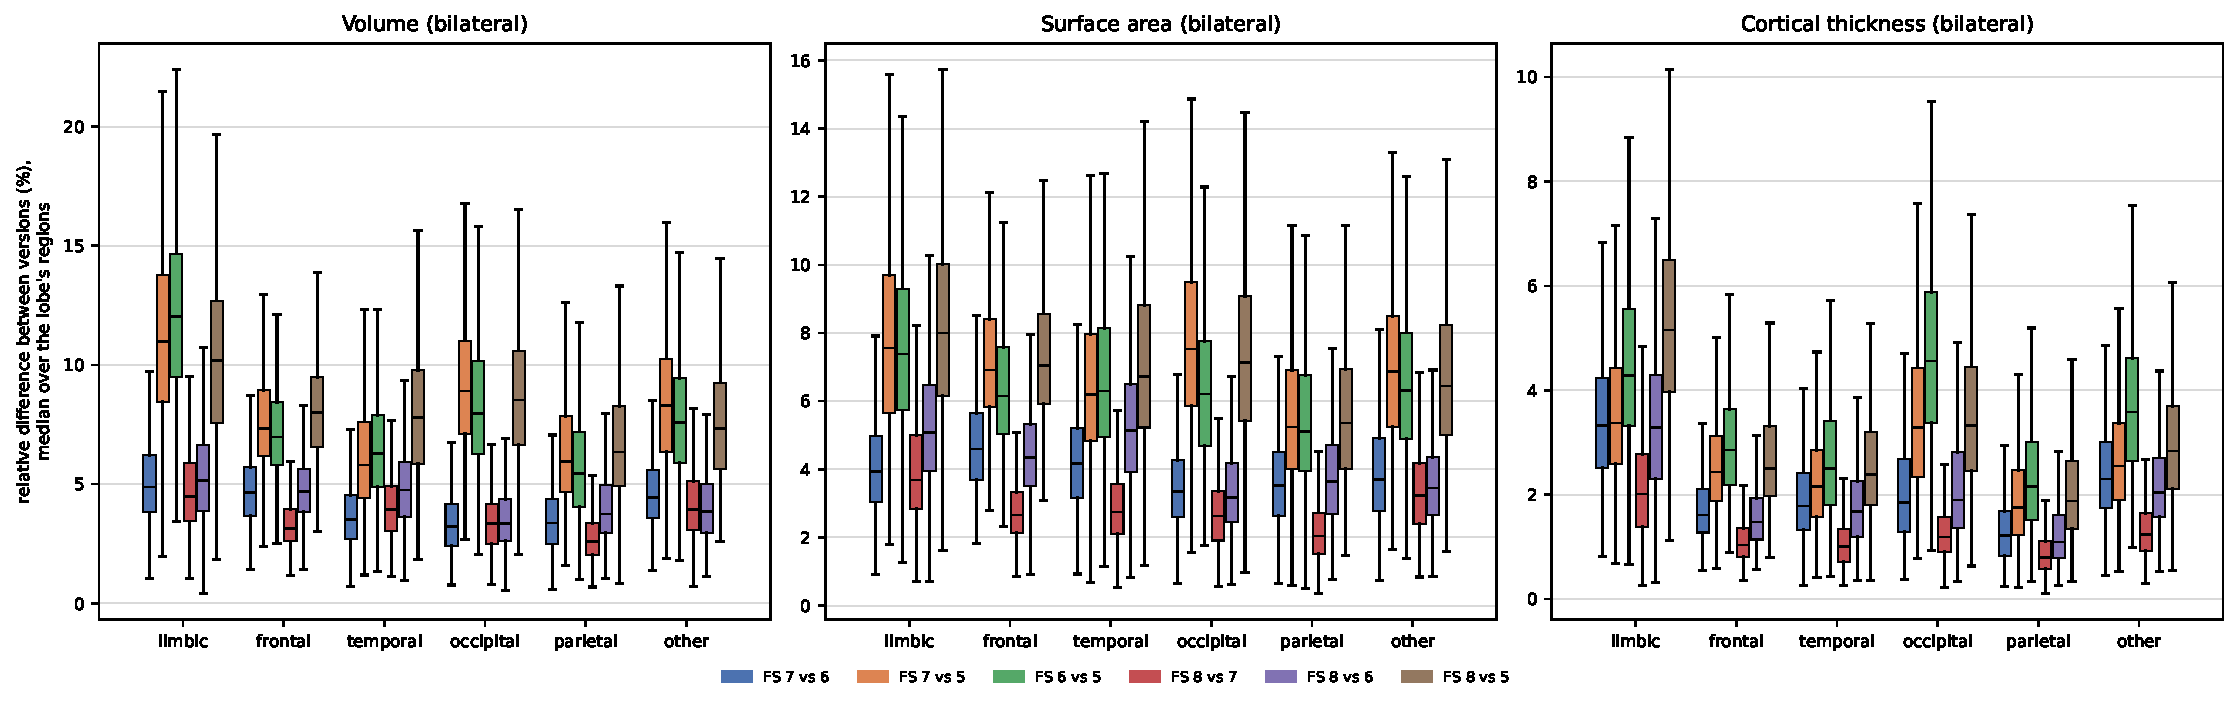
\includegraphics[width=\linewidth,height=0.8\textheight,keepaspectratio]{variability_by_type_cortical}
\caption{\rev{Relative differences between FreeSurfer versions in cortical volume, surface area and thickness by
lobe (Destrieux atlas, bilateral measures: mean of the two hemispheres for thickness and volume, sum for surface
area; 830 images). For each image, the median of $|A - B|/B$ (\%) over the regions of the lobe; ``other'': insular
and boundary regions.}}
\end{figure}

\begin{figure}[p]
\centering
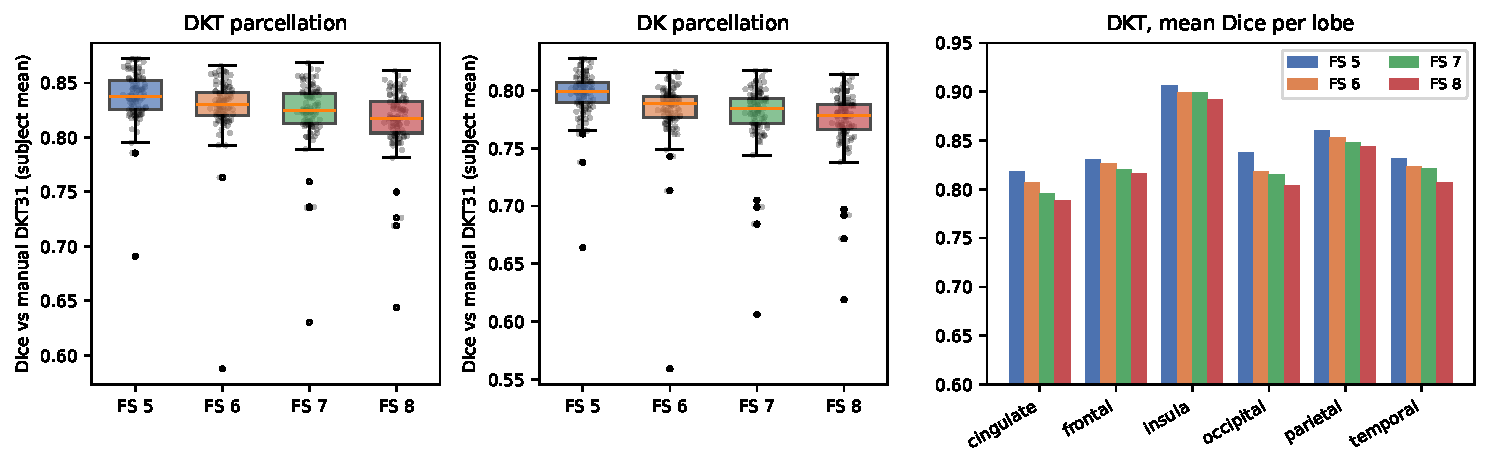
\includegraphics[width=\linewidth]{mindboggle_dice}
\caption{\rev{Accuracy of the cortical parcellation of each FreeSurfer version against the manual DKT31 labels of
Mindboggle-101 (101 images). Left and middle: Sørensen--Dice coefficient of each image (mean over the 62 DKT31
regions) for the DKT and DK parcellations, resampled to the native T1-weighted space. Right: mean Dice per lobe, DKT
parcellation. The DKT atlas of FS5 was built from 40 of the Mindboggle-101 images.}}\label{fig:S7}
\end{figure}

\clearpage
\begin{landscape}
{\scriptsize\setlength{\tabcolsep}{3pt}
\begin{longtable}{llrrrrrrrrrrrr}
\caption{Differences between FreeSurfer versions, all images (n = 830). Paired t-tests between versions; raw $p$, $^{*}$ significant after Bonferroni correction ($\alpha = 0.05/187$ for volume, $0.05/148$ for surface area and thickness). $^{\dagger}$Label not produced by FS8 (volume 0 in every image): significant by construction in the FS8 comparisons.}\label{tab:S1}\\
\toprule
Region & & \multicolumn{2}{c}{7 vs 6} & \multicolumn{2}{c}{7 vs 5} & \multicolumn{2}{c}{6 vs 5} & \multicolumn{2}{c}{8 vs 7} & \multicolumn{2}{c}{8 vs 6} & \multicolumn{2}{c}{8 vs 5} \\
Region & & $t$ & $p$ & $t$ & $p$ & $t$ & $p$ & $t$ & $p$ & $t$ & $p$ & $t$ & $p$ \\
\midrule\endfirsthead
\toprule
Region & & \multicolumn{2}{c}{7 vs 6} & \multicolumn{2}{c}{7 vs 5} & \multicolumn{2}{c}{6 vs 5} & \multicolumn{2}{c}{8 vs 7} & \multicolumn{2}{c}{8 vs 6} & \multicolumn{2}{c}{8 vs 5} \\
Region & & $t$ & $p$ & $t$ & $p$ & $t$ & $p$ & $t$ & $p$ & $t$ & $p$ & $t$ & $p$ \\
\midrule\endhead
\bottomrule\endfoot
\midrule\multicolumn{14}{l}{\textbf{Volume (subcortical)}} \\
Left-Lateral-Ventricle &  & -0.49 & 0.622 & 15.90 & $<$0.001$^{*}$ & 16.86 & $<$0.001$^{*}$ & 14.51 & $<$0.001$^{*}$ & 16.03 & $<$0.001$^{*}$ & 23.51 & $<$0.001$^{*}$ \\
Left-Inf-Lat-Vent &  & 3.89 & $<$0.001$^{*}$ & 5.70 & $<$0.001$^{*}$ & 2.89 & 0.004 & 40.23 & $<$0.001$^{*}$ & 43.21 & $<$0.001$^{*}$ & 42.40 & $<$0.001$^{*}$ \\
Left-Cerebellum-White-Matter &  & -5.85 & $<$0.001$^{*}$ & -22.38 & $<$0.001$^{*}$ & -17.02 & $<$0.001$^{*}$ & 4.07 & $<$0.001$^{*}$ & -0.74 & 0.461 & -13.62 & $<$0.001$^{*}$ \\
Left-Cerebellum-Cortex &  & 3.14 & 0.002 & 71.45 & $<$0.001$^{*}$ & 70.59 & $<$0.001$^{*}$ & -7.70 & $<$0.001$^{*}$ & -5.67 & $<$0.001$^{*}$ & 42.83 & $<$0.001$^{*}$ \\
Left-Thalamus &  & 16.14 & $<$0.001$^{*}$ & -10.24 & $<$0.001$^{*}$ & -19.57 & $<$0.001$^{*}$ & -10.92 & $<$0.001$^{*}$ & 1.51 & 0.131 & -17.61 & $<$0.001$^{*}$ \\
Left-Caudate &  & 6.78 & $<$0.001$^{*}$ & -22.02 & $<$0.001$^{*}$ & -27.43 & $<$0.001$^{*}$ & 38.51 & $<$0.001$^{*}$ & 42.93 & $<$0.001$^{*}$ & 12.49 & $<$0.001$^{*}$ \\
Left-Putamen &  & 10.61 & $<$0.001$^{*}$ & -45.66 & $<$0.001$^{*}$ & -53.81 & $<$0.001$^{*}$ & 65.25 & $<$0.001$^{*}$ & 73.43 & $<$0.001$^{*}$ & -0.94 & 0.345 \\
Left-Pallidum &  & 3.90 & $<$0.001$^{*}$ & 72.12 & $<$0.001$^{*}$ & 73.36 & $<$0.001$^{*}$ & -55.52 & $<$0.001$^{*}$ & -56.13 & $<$0.001$^{*}$ & 29.70 & $<$0.001$^{*}$ \\
3rd-Ventricle &  & -1.04 & 0.298 & 10.49 & $<$0.001$^{*}$ & 12.28 & $<$0.001$^{*}$ & -2.83 & 0.005 & -5.36 & $<$0.001$^{*}$ & 5.55 & $<$0.001$^{*}$ \\
4th-Ventricle &  & 8.03 & $<$0.001$^{*}$ & -15.43 & $<$0.001$^{*}$ & -18.39 & $<$0.001$^{*}$ & 71.84 & $<$0.001$^{*}$ & 70.64 & $<$0.001$^{*}$ & 45.52 & $<$0.001$^{*}$ \\
Brain-Stem &  & 22.09 & $<$0.001$^{*}$ & 6.95 & $<$0.001$^{*}$ & -9.79 & $<$0.001$^{*}$ & 4.71 & $<$0.001$^{*}$ & 21.41 & $<$0.001$^{*}$ & 10.72 & $<$0.001$^{*}$ \\
Left-Hippocampus &  & 22.73 & $<$0.001$^{*}$ & 14.68 & $<$0.001$^{*}$ & 2.84 & 0.005 & 27.00 & $<$0.001$^{*}$ & 39.06 & $<$0.001$^{*}$ & 32.22 & $<$0.001$^{*}$ \\
Left-Amygdala &  & 12.10 & $<$0.001$^{*}$ & 13.42 & $<$0.001$^{*}$ & 5.05 & $<$0.001$^{*}$ & 32.29 & $<$0.001$^{*}$ & 45.02 & $<$0.001$^{*}$ & 39.62 & $<$0.001$^{*}$ \\
CSF &  & -3.86 & $<$0.001$^{*}$ & -14.52 & $<$0.001$^{*}$ & -14.14 & $<$0.001$^{*}$ & 186.59 & $<$0.001$^{*}$ & 186.54 & $<$0.001$^{*}$ & 186.50 & $<$0.001$^{*}$ \\
Left-Accumbens-area &  & -9.29 & $<$0.001$^{*}$ & -9.20 & $<$0.001$^{*}$ & -3.57 & $<$0.001 & 62.45 & $<$0.001$^{*}$ & 60.46 & $<$0.001$^{*}$ & 39.73 & $<$0.001$^{*}$ \\
Left-VentralDC &  & -3.83 & $<$0.001$^{*}$ & 23.24 & $<$0.001$^{*}$ & 28.29 & $<$0.001$^{*}$ & 1.40 & 0.161 & -1.20 & 0.232 & 24.36 & $<$0.001$^{*}$ \\
Left-vessel$^{\dagger}$ &  & -3.91 & $<$0.001$^{*}$ & -49.37 & $<$0.001$^{*}$ & -47.97 & $<$0.001$^{*}$ & -33.97 & $<$0.001$^{*}$ & -32.93 & $<$0.001$^{*}$ & -55.69 & $<$0.001$^{*}$ \\
Left-choroid-plexus$^{\dagger}$ &  & 0.19 & 0.850 & -90.86 & $<$0.001$^{*}$ & -91.67 & $<$0.001$^{*}$ & -86.71 & $<$0.001$^{*}$ & -84.62 & $<$0.001$^{*}$ & -129.32 & $<$0.001$^{*}$ \\
Right-Lateral-Ventricle &  & -1.51 & 0.132 & 9.72 & $<$0.001$^{*}$ & 10.57 & $<$0.001$^{*}$ & 15.16 & $<$0.001$^{*}$ & 17.41 & $<$0.001$^{*}$ & 19.39 & $<$0.001$^{*}$ \\
Right-Inf-Lat-Vent &  & 7.50 & $<$0.001$^{*}$ & 22.36 & $<$0.001$^{*}$ & 18.08 & $<$0.001$^{*}$ & 42.25 & $<$0.001$^{*}$ & 46.95 & $<$0.001$^{*}$ & 58.42 & $<$0.001$^{*}$ \\
Right-Cerebellum-White-Matter &  & -7.45 & $<$0.001$^{*}$ & -34.81 & $<$0.001$^{*}$ & -32.23 & $<$0.001$^{*}$ & 20.14 & $<$0.001$^{*}$ & 13.71 & $<$0.001$^{*}$ & -12.98 & $<$0.001$^{*}$ \\
Right-Cerebellum-Cortex &  & 8.22 & $<$0.001$^{*}$ & 61.04 & $<$0.001$^{*}$ & 61.80 & $<$0.001$^{*}$ & -22.86 & $<$0.001$^{*}$ & -18.32 & $<$0.001$^{*}$ & 26.77 & $<$0.001$^{*}$ \\
Right-Thalamus &  & 23.67 & $<$0.001$^{*}$ & 25.20 & $<$0.001$^{*}$ & 10.94 & $<$0.001$^{*}$ & -24.25 & $<$0.001$^{*}$ & -6.06 & $<$0.001$^{*}$ & 3.16 & 0.002 \\
Right-Caudate &  & 3.77 & $<$0.001$^{*}$ & -16.96 & $<$0.001$^{*}$ & -20.49 & $<$0.001$^{*}$ & 36.76 & $<$0.001$^{*}$ & 41.07 & $<$0.001$^{*}$ & 10.56 & $<$0.001$^{*}$ \\
Right-Putamen &  & 12.63 & $<$0.001$^{*}$ & -18.14 & $<$0.001$^{*}$ & -25.32 & $<$0.001$^{*}$ & 48.12 & $<$0.001$^{*}$ & 61.06 & $<$0.001$^{*}$ & 13.51 & $<$0.001$^{*}$ \\
Right-Pallidum &  & 2.92 & 0.004 & 65.76 & $<$0.001$^{*}$ & 71.51 & $<$0.001$^{*}$ & -49.80 & $<$0.001$^{*}$ & -50.44 & $<$0.001$^{*}$ & 25.41 & $<$0.001$^{*}$ \\
Right-Hippocampus &  & 18.05 & $<$0.001$^{*}$ & 8.19 & $<$0.001$^{*}$ & -2.40 & 0.017 & 29.00 & $<$0.001$^{*}$ & 41.37 & $<$0.001$^{*}$ & 29.09 & $<$0.001$^{*}$ \\
Right-Amygdala &  & 4.06 & $<$0.001$^{*}$ & 20.91 & $<$0.001$^{*}$ & 19.06 & $<$0.001$^{*}$ & 20.23 & $<$0.001$^{*}$ & 22.95 & $<$0.001$^{*}$ & 32.52 & $<$0.001$^{*}$ \\
Right-Accumbens-area &  & 4.50 & $<$0.001$^{*}$ & -8.35 & $<$0.001$^{*}$ & -11.62 & $<$0.001$^{*}$ & 52.68 & $<$0.001$^{*}$ & 63.11 & $<$0.001$^{*}$ & 34.34 & $<$0.001$^{*}$ \\
Right-VentralDC &  & 0.51 & 0.614 & 27.40 & $<$0.001$^{*}$ & 30.63 & $<$0.001$^{*}$ & 9.91 & $<$0.001$^{*}$ & 11.87 & $<$0.001$^{*}$ & 34.31 & $<$0.001$^{*}$ \\
Right-vessel$^{\dagger}$ &  & -4.22 & $<$0.001$^{*}$ & -45.76 & $<$0.001$^{*}$ & -42.83 & $<$0.001$^{*}$ & -17.96 & $<$0.001$^{*}$ & -18.25 & $<$0.001$^{*}$ & -51.54 & $<$0.001$^{*}$ \\
Right-choroid-plexus$^{\dagger}$ &  & 3.56 & $<$0.001 & -86.66 & $<$0.001$^{*}$ & -91.22 & $<$0.001$^{*}$ & -91.42 & $<$0.001$^{*}$ & -83.45 & $<$0.001$^{*}$ & -101.42 & $<$0.001$^{*}$ \\
5th-Ventricle$^{\dagger}$ &  & -1.27 & 0.203 & -15.98 & $<$0.001$^{*}$ & -15.93 & $<$0.001$^{*}$ & -2.63 & 0.009 & -3.45 & $<$0.001 & -16.06 & $<$0.001$^{*}$ \\
Optic-Chiasm$^{\dagger}$ &  & -11.54 & $<$0.001$^{*}$ & -23.20 & $<$0.001$^{*}$ & -14.16 & $<$0.001$^{*}$ & -135.61 & $<$0.001$^{*}$ & -114.33 & $<$0.001$^{*}$ & -104.39 & $<$0.001$^{*}$ \\
CC\_Posterior &  & -4.77 & $<$0.001$^{*}$ & 17.57 & $<$0.001$^{*}$ & 20.83 & $<$0.001$^{*}$ & -5.20 & $<$0.001$^{*}$ & -9.37 & $<$0.001$^{*}$ & 16.57 & $<$0.001$^{*}$ \\
CC\_Mid\_Posterior &  & -7.71 & $<$0.001$^{*}$ & 42.89 & $<$0.001$^{*}$ & 43.22 & $<$0.001$^{*}$ & -15.50 & $<$0.001$^{*}$ & -18.22 & $<$0.001$^{*}$ & 39.51 & $<$0.001$^{*}$ \\
CC\_Central &  & -3.43 & $<$0.001 & 31.90 & $<$0.001$^{*}$ & 33.84 & $<$0.001$^{*}$ & 27.78 & $<$0.001$^{*}$ & 26.58 & $<$0.001$^{*}$ & 49.66 & $<$0.001$^{*}$ \\
CC\_Mid\_Anterior &  & -3.54 & $<$0.001 & 30.62 & $<$0.001$^{*}$ & 31.73 & $<$0.001$^{*}$ & -17.37 & $<$0.001$^{*}$ & -17.93 & $<$0.001$^{*}$ & 14.36 & $<$0.001$^{*}$ \\
CC\_Anterior &  & -2.39 & 0.017 & 25.60 & $<$0.001$^{*}$ & 28.77 & $<$0.001$^{*}$ & 18.97 & $<$0.001$^{*}$ & 17.68 & $<$0.001$^{*}$ & 40.34 & $<$0.001$^{*}$ \\
\midrule\multicolumn{14}{l}{\textbf{Volume, lh}} \\
G\_and\_S\_frontomargin &  & 3.28 & 0.001 & 25.00 & $<$0.001$^{*}$ & 24.02 & $<$0.001$^{*}$ & 15.52 & $<$0.001$^{*}$ & 17.50 & $<$0.001$^{*}$ & 34.46 & $<$0.001$^{*}$ \\
G\_and\_S\_occipital\_inf &  & 0.07 & 0.948 & 14.68 & $<$0.001$^{*}$ & 15.09 & $<$0.001$^{*}$ & -5.53 & $<$0.001$^{*}$ & -5.12 & $<$0.001$^{*}$ & 10.52 & $<$0.001$^{*}$ \\
G\_and\_S\_paracentral &  & 13.48 & $<$0.001$^{*}$ & 22.97 & $<$0.001$^{*}$ & 15.22 & $<$0.001$^{*}$ & -4.50 & $<$0.001$^{*}$ & 10.12 & $<$0.001$^{*}$ & 20.71 & $<$0.001$^{*}$ \\
G\_and\_S\_subcentral &  & 5.40 & $<$0.001$^{*}$ & 12.59 & $<$0.001$^{*}$ & 8.52 & $<$0.001$^{*}$ & 8.94 & $<$0.001$^{*}$ & 13.36 & $<$0.001$^{*}$ & 17.62 & $<$0.001$^{*}$ \\
G\_and\_S\_transv\_frontopol &  & 15.30 & $<$0.001$^{*}$ & 27.70 & $<$0.001$^{*}$ & 18.41 & $<$0.001$^{*}$ & 8.43 & $<$0.001$^{*}$ & 22.34 & $<$0.001$^{*}$ & 34.16 & $<$0.001$^{*}$ \\
G\_and\_S\_cingul-Ant &  & 8.00 & $<$0.001$^{*}$ & 3.17 & 0.002 & -2.17 & 0.030 & 15.14 & $<$0.001$^{*}$ & 21.72 & $<$0.001$^{*}$ & 12.08 & $<$0.001$^{*}$ \\
G\_and\_S\_cingul-Mid-Ant &  & -9.18 & $<$0.001$^{*}$ & -27.47 & $<$0.001$^{*}$ & -24.00 & $<$0.001$^{*}$ & 7.56 & $<$0.001$^{*}$ & -2.27 & 0.024 & -24.31 & $<$0.001$^{*}$ \\
G\_and\_S\_cingul-Mid-Post &  & -14.10 & $<$0.001$^{*}$ & 6.46 & $<$0.001$^{*}$ & 16.65 & $<$0.001$^{*}$ & 8.43 & $<$0.001$^{*}$ & -8.12 & $<$0.001$^{*}$ & 12.79 & $<$0.001$^{*}$ \\
G\_cingul-Post-dorsal &  & -16.87 & $<$0.001$^{*}$ & 21.98 & $<$0.001$^{*}$ & 33.13 & $<$0.001$^{*}$ & 7.01 & $<$0.001$^{*}$ & -9.31 & $<$0.001$^{*}$ & 26.56 & $<$0.001$^{*}$ \\
G\_cingul-Post-ventral &  & -5.07 & $<$0.001$^{*}$ & 13.39 & $<$0.001$^{*}$ & 15.14 & $<$0.001$^{*}$ & 10.61 & $<$0.001$^{*}$ & 4.62 & $<$0.001$^{*}$ & 15.57 & $<$0.001$^{*}$ \\
G\_cuneus &  & -0.10 & 0.920 & 33.81 & $<$0.001$^{*}$ & 35.61 & $<$0.001$^{*}$ & -2.01 & 0.045 & -1.66 & 0.097 & 32.26 & $<$0.001$^{*}$ \\
G\_front\_inf-Opercular &  & 6.27 & $<$0.001$^{*}$ & -8.15 & $<$0.001$^{*}$ & -12.48 & $<$0.001$^{*}$ & 8.47 & $<$0.001$^{*}$ & 14.79 & $<$0.001$^{*}$ & -2.38 & 0.018 \\
G\_front\_inf-Orbital &  & 9.63 & $<$0.001$^{*}$ & 57.66 & $<$0.001$^{*}$ & 51.88 & $<$0.001$^{*}$ & 2.05 & 0.041 & 11.64 & $<$0.001$^{*}$ & 60.44 & $<$0.001$^{*}$ \\
G\_front\_inf-Triangul &  & 4.79 & $<$0.001$^{*}$ & 2.23 & 0.026 & -0.71 & 0.479 & 11.03 & $<$0.001$^{*}$ & 14.70 & $<$0.001$^{*}$ & 7.68 & $<$0.001$^{*}$ \\
G\_front\_middle &  & -0.74 & 0.459 & 5.87 & $<$0.001$^{*}$ & 6.87 & $<$0.001$^{*}$ & 10.53 & $<$0.001$^{*}$ & 10.32 & $<$0.001$^{*}$ & 13.84 & $<$0.001$^{*}$ \\
G\_front\_sup &  & 12.07 & $<$0.001$^{*}$ & 28.67 & $<$0.001$^{*}$ & 21.77 & $<$0.001$^{*}$ & 7.03 & $<$0.001$^{*}$ & 19.45 & $<$0.001$^{*}$ & 33.00 & $<$0.001$^{*}$ \\
G\_Ins\_lg\_and\_S\_cent\_ins &  & -4.83 & $<$0.001$^{*}$ & 67.80 & $<$0.001$^{*}$ & 57.85 & $<$0.001$^{*}$ & -12.90 & $<$0.001$^{*}$ & -14.06 & $<$0.001$^{*}$ & 59.76 & $<$0.001$^{*}$ \\
G\_insular\_short &  & 4.70 & $<$0.001$^{*}$ & 29.82 & $<$0.001$^{*}$ & 25.04 & $<$0.001$^{*}$ & -13.87 & $<$0.001$^{*}$ & -7.23 & $<$0.001$^{*}$ & 20.95 & $<$0.001$^{*}$ \\
G\_occipital\_middle &  & 2.59 & 0.010 & 15.26 & $<$0.001$^{*}$ & 14.74 & $<$0.001$^{*}$ & 8.86 & $<$0.001$^{*}$ & 11.23 & $<$0.001$^{*}$ & 19.25 & $<$0.001$^{*}$ \\
G\_occipital\_sup &  & 2.56 & 0.011 & -15.97 & $<$0.001$^{*}$ & -18.18 & $<$0.001$^{*}$ & 1.05 & 0.295 & 3.08 & 0.002 & -14.54 & $<$0.001$^{*}$ \\
G\_oc-temp\_lat-fusifor &  & 2.84 & 0.005 & 4.78 & $<$0.001$^{*}$ & 3.31 & $<$0.001 & 20.00 & $<$0.001$^{*}$ & 27.43 & $<$0.001$^{*}$ & 19.07 & $<$0.001$^{*}$ \\
G\_oc-temp\_med-Lingual &  & 2.27 & 0.023 & 23.76 & $<$0.001$^{*}$ & 22.97 & $<$0.001$^{*}$ & 5.96 & $<$0.001$^{*}$ & 7.05 & $<$0.001$^{*}$ & 25.12 & $<$0.001$^{*}$ \\
G\_oc-temp\_med-Parahip &  & -22.39 & $<$0.001$^{*}$ & 13.82 & $<$0.001$^{*}$ & 28.40 & $<$0.001$^{*}$ & 11.87 & $<$0.001$^{*}$ & -10.40 & $<$0.001$^{*}$ & 22.74 & $<$0.001$^{*}$ \\
G\_orbital &  & 3.39 & $<$0.001 & 4.21 & $<$0.001$^{*}$ & 1.77 & 0.077 & 3.17 & 0.002 & 6.59 & $<$0.001$^{*}$ & 5.99 & $<$0.001$^{*}$ \\
G\_pariet\_inf-Angular &  & 6.55 & $<$0.001$^{*}$ & 17.75 & $<$0.001$^{*}$ & 14.04 & $<$0.001$^{*}$ & 10.22 & $<$0.001$^{*}$ & 15.80 & $<$0.001$^{*}$ & 22.88 & $<$0.001$^{*}$ \\
G\_pariet\_inf-Supramar &  & 5.89 & $<$0.001$^{*}$ & 0.24 & 0.808 & -4.46 & $<$0.001$^{*}$ & 10.00 & $<$0.001$^{*}$ & 15.10 & $<$0.001$^{*}$ & 6.77 & $<$0.001$^{*}$ \\
G\_parietal\_sup &  & 6.79 & $<$0.001$^{*}$ & 9.78 & $<$0.001$^{*}$ & 5.38 & $<$0.001$^{*}$ & 11.25 & $<$0.001$^{*}$ & 17.85 & $<$0.001$^{*}$ & 16.38 & $<$0.001$^{*}$ \\
G\_postcentral &  & 22.27 & $<$0.001$^{*}$ & 9.19 & $<$0.001$^{*}$ & -4.33 & $<$0.001$^{*}$ & 10.47 & $<$0.001$^{*}$ & 30.99 & $<$0.001$^{*}$ & 15.63 & $<$0.001$^{*}$ \\
G\_precentral &  & 18.02 & $<$0.001$^{*}$ & -2.54 & 0.011 & -16.20 & $<$0.001$^{*}$ & 9.47 & $<$0.001$^{*}$ & 27.08 & $<$0.001$^{*}$ & 2.98 & 0.003 \\
G\_precuneus &  & 1.85 & 0.065 & 24.38 & $<$0.001$^{*}$ & 21.96 & $<$0.001$^{*}$ & 12.70 & $<$0.001$^{*}$ & 12.75 & $<$0.001$^{*}$ & 31.68 & $<$0.001$^{*}$ \\
G\_rectus &  & 18.54 & $<$0.001$^{*}$ & 11.76 & $<$0.001$^{*}$ & -3.46 & $<$0.001 & 15.21 & $<$0.001$^{*}$ & 30.28 & $<$0.001$^{*}$ & 21.58 & $<$0.001$^{*}$ \\
G\_subcallosal &  & -10.22 & $<$0.001$^{*}$ & 35.39 & $<$0.001$^{*}$ & 37.23 & $<$0.001$^{*}$ & -7.57 & $<$0.001$^{*}$ & -14.74 & $<$0.001$^{*}$ & 27.18 & $<$0.001$^{*}$ \\
G\_temp\_sup-G\_T\_transv &  & 7.26 & $<$0.001$^{*}$ & -1.45 & 0.148 & -6.64 & $<$0.001$^{*}$ & 19.23 & $<$0.001$^{*}$ & 23.12 & $<$0.001$^{*}$ & 10.35 & $<$0.001$^{*}$ \\
G\_temp\_sup-Lateral &  & 10.83 & $<$0.001$^{*}$ & 1.55 & 0.122 & -7.49 & $<$0.001$^{*}$ & 35.01 & $<$0.001$^{*}$ & 38.86 & $<$0.001$^{*}$ & 25.29 & $<$0.001$^{*}$ \\
G\_temp\_sup-Plan\_polar &  & 2.90 & 0.004 & 40.32 & $<$0.001$^{*}$ & 40.77 & $<$0.001$^{*}$ & 2.00 & 0.046 & 4.95 & $<$0.001$^{*}$ & 43.05 & $<$0.001$^{*}$ \\
G\_temp\_sup-Plan\_tempo &  & -8.95 & $<$0.001$^{*}$ & 6.33 & $<$0.001$^{*}$ & 11.59 & $<$0.001$^{*}$ & 7.23 & $<$0.001$^{*}$ & -1.55 & 0.122 & 10.46 & $<$0.001$^{*}$ \\
G\_temporal\_inf &  & 3.63 & $<$0.001 & 2.35 & 0.019 & -0.29 & 0.772 & 18.66 & $<$0.001$^{*}$ & 20.48 & $<$0.001$^{*}$ & 13.80 & $<$0.001$^{*}$ \\
G\_temporal\_middle &  & 6.73 & $<$0.001$^{*}$ & -19.50 & $<$0.001$^{*}$ & -22.89 & $<$0.001$^{*}$ & 21.01 & $<$0.001$^{*}$ & 23.64 & $<$0.001$^{*}$ & -7.13 & $<$0.001$^{*}$ \\
Lat\_Fis-ant-Horizont &  & -6.36 & $<$0.001$^{*}$ & -16.33 & $<$0.001$^{*}$ & -11.04 & $<$0.001$^{*}$ & 0.59 & 0.553 & -6.17 & $<$0.001$^{*}$ & -15.91 & $<$0.001$^{*}$ \\
Lat\_Fis-ant-Vertical &  & -8.81 & $<$0.001$^{*}$ & 9.22 & $<$0.001$^{*}$ & 15.55 & $<$0.001$^{*}$ & 2.95 & 0.003 & -6.71 & $<$0.001$^{*}$ & 11.54 & $<$0.001$^{*}$ \\
Lat\_Fis-post &  & -10.19 & $<$0.001$^{*}$ & -25.34 & $<$0.001$^{*}$ & -16.26 & $<$0.001$^{*}$ & 11.42 & $<$0.001$^{*}$ & -1.28 & 0.201 & -17.29 & $<$0.001$^{*}$ \\
Pole\_occipital &  & 9.16 & $<$0.001$^{*}$ & 7.12 & $<$0.001$^{*}$ & 1.16 & 0.247 & -6.86 & $<$0.001$^{*}$ & 1.54 & 0.124 & 2.22 & 0.027 \\
Pole\_temporal &  & 19.17 & $<$0.001$^{*}$ & 10.06 & $<$0.001$^{*}$ & -3.08 & 0.002 & -8.10 & $<$0.001$^{*}$ & 12.04 & $<$0.001$^{*}$ & 5.26 & $<$0.001$^{*}$ \\
S\_calcarine &  & -10.30 & $<$0.001$^{*}$ & -11.38 & $<$0.001$^{*}$ & -4.15 & $<$0.001$^{*}$ & 20.86 & $<$0.001$^{*}$ & 8.72 & $<$0.001$^{*}$ & 2.49 & 0.013 \\
S\_central &  & -43.47 & $<$0.001$^{*}$ & -13.38 & $<$0.001$^{*}$ & 20.72 & $<$0.001$^{*}$ & 9.76 & $<$0.001$^{*}$ & -33.38 & $<$0.001$^{*}$ & -7.37 & $<$0.001$^{*}$ \\
S\_cingul-Marginalis &  & -22.89 & $<$0.001$^{*}$ & -21.03 & $<$0.001$^{*}$ & -5.97 & $<$0.001$^{*}$ & -0.13 & 0.899 & -23.67 & $<$0.001$^{*}$ & -20.84 & $<$0.001$^{*}$ \\
S\_circular\_insula\_ant &  & -8.74 & $<$0.001$^{*}$ & -11.57 & $<$0.001$^{*}$ & -3.72 & $<$0.001$^{*}$ & -4.41 & $<$0.001$^{*}$ & -13.51 & $<$0.001$^{*}$ & -15.04 & $<$0.001$^{*}$ \\
S\_circular\_insula\_inf &  & -5.59 & $<$0.001$^{*}$ & -19.36 & $<$0.001$^{*}$ & -12.70 & $<$0.001$^{*}$ & 25.99 & $<$0.001$^{*}$ & 18.54 & $<$0.001$^{*}$ & 2.02 & 0.043 \\
S\_circular\_insula\_sup &  & -12.12 & $<$0.001$^{*}$ & -34.81 & $<$0.001$^{*}$ & -19.23 & $<$0.001$^{*}$ & 12.29 & $<$0.001$^{*}$ & -2.59 & 0.010 & -23.66 & $<$0.001$^{*}$ \\
S\_collat\_transv\_ant &  & -4.80 & $<$0.001$^{*}$ & 0.73 & 0.468 & 4.05 & $<$0.001$^{*}$ & 17.84 & $<$0.001$^{*}$ & 12.49 & $<$0.001$^{*}$ & 12.13 & $<$0.001$^{*}$ \\
S\_collat\_transv\_post &  & -6.74 & $<$0.001$^{*}$ & 16.54 & $<$0.001$^{*}$ & 20.74 & $<$0.001$^{*}$ & 2.08 & 0.038 & -4.46 & $<$0.001$^{*}$ & 18.12 & $<$0.001$^{*}$ \\
S\_front\_inf &  & -9.09 & $<$0.001$^{*}$ & -10.73 & $<$0.001$^{*}$ & -3.79 & $<$0.001$^{*}$ & 9.70 & $<$0.001$^{*}$ & -1.28 & 0.200 & -4.47 & $<$0.001$^{*}$ \\
S\_front\_middle &  & -8.14 & $<$0.001$^{*}$ & -19.01 & $<$0.001$^{*}$ & -15.26 & $<$0.001$^{*}$ & 8.87 & $<$0.001$^{*}$ & -0.24 & 0.813 & -14.53 & $<$0.001$^{*}$ \\
S\_front\_sup &  & -11.81 & $<$0.001$^{*}$ & 5.58 & $<$0.001$^{*}$ & 15.31 & $<$0.001$^{*}$ & 5.79 & $<$0.001$^{*}$ & -6.53 & $<$0.001$^{*}$ & 9.60 & $<$0.001$^{*}$ \\
S\_interm\_prim-Jensen &  & -8.17 & $<$0.001$^{*}$ & -5.97 & $<$0.001$^{*}$ & -2.23 & 0.026 & 3.96 & $<$0.001$^{*}$ & -5.02 & $<$0.001$^{*}$ & -4.44 & $<$0.001$^{*}$ \\
S\_intrapariet\_and\_P\_trans &  & -16.57 & $<$0.001$^{*}$ & -24.27 & $<$0.001$^{*}$ & -12.15 & $<$0.001$^{*}$ & 11.35 & $<$0.001$^{*}$ & -9.28 & $<$0.001$^{*}$ & -18.72 & $<$0.001$^{*}$ \\
S\_oc\_middle\_and\_Lunatus &  & -11.06 & $<$0.001$^{*}$ & -14.39 & $<$0.001$^{*}$ & -8.34 & $<$0.001$^{*}$ & 12.11 & $<$0.001$^{*}$ & -0.47 & 0.642 & -8.39 & $<$0.001$^{*}$ \\
S\_oc\_sup\_and\_transversal &  & -15.35 & $<$0.001$^{*}$ & -7.42 & $<$0.001$^{*}$ & 1.13 & 0.257 & 13.71 & $<$0.001$^{*}$ & -2.71 & 0.007 & -0.43 & 0.667 \\
S\_occipital\_ant &  & -3.10 & 0.002 & -7.01 & $<$0.001$^{*}$ & -5.50 & $<$0.001$^{*}$ & 3.27 & 0.001 & 0.03 & 0.973 & -5.26 & $<$0.001$^{*}$ \\
S\_oc-temp\_lat &  & -9.16 & $<$0.001$^{*}$ & -1.23 & 0.219 & 5.20 & $<$0.001$^{*}$ & 6.78 & $<$0.001$^{*}$ & -2.91 & 0.004 & 3.37 & $<$0.001 \\
S\_oc-temp\_med\_and\_Lingual &  & -17.23 & $<$0.001$^{*}$ & -9.58 & $<$0.001$^{*}$ & 0.02 & 0.982 & 16.05 & $<$0.001$^{*}$ & -2.97 & 0.003 & -1.63 & 0.104 \\
S\_orbital\_lateral &  & -12.15 & $<$0.001$^{*}$ & -17.06 & $<$0.001$^{*}$ & -8.15 & $<$0.001$^{*}$ & 6.14 & $<$0.001$^{*}$ & -6.26 & $<$0.001$^{*}$ & -12.34 & $<$0.001$^{*}$ \\
S\_orbital\_med-olfact &  & 11.01 & $<$0.001$^{*}$ & -34.14 & $<$0.001$^{*}$ & -37.97 & $<$0.001$^{*}$ & -18.78 & $<$0.001$^{*}$ & -4.91 & $<$0.001$^{*}$ & -40.44 & $<$0.001$^{*}$ \\
S\_orbital-H\_Shaped &  & -21.57 & $<$0.001$^{*}$ & 24.58 & $<$0.001$^{*}$ & 39.69 & $<$0.001$^{*}$ & 7.82 & $<$0.001$^{*}$ & -15.14 & $<$0.001$^{*}$ & 28.37 & $<$0.001$^{*}$ \\
S\_parieto\_occipital &  & -13.85 & $<$0.001$^{*}$ & 13.48 & $<$0.001$^{*}$ & 21.82 & $<$0.001$^{*}$ & 8.77 & $<$0.001$^{*}$ & -5.57 & $<$0.001$^{*}$ & 18.15 & $<$0.001$^{*}$ \\
S\_pericallosal &  & -2.83 & 0.005 & -15.89 & $<$0.001$^{*}$ & -10.01 & $<$0.001$^{*}$ & 12.90 & $<$0.001$^{*}$ & 10.20 & $<$0.001$^{*}$ & -0.33 & 0.738 \\
S\_postcentral &  & -15.53 & $<$0.001$^{*}$ & 2.66 & 0.008 & 12.82 & $<$0.001$^{*}$ & 6.63 & $<$0.001$^{*}$ & -10.72 & $<$0.001$^{*}$ & 6.14 & $<$0.001$^{*}$ \\
S\_precentral-inf-part &  & -13.63 & $<$0.001$^{*}$ & 15.32 & $<$0.001$^{*}$ & 25.00 & $<$0.001$^{*}$ & 2.69 & 0.007 & -14.20 & $<$0.001$^{*}$ & 16.39 & $<$0.001$^{*}$ \\
S\_precentral-sup-part &  & -26.77 & $<$0.001$^{*}$ & -0.54 & 0.592 & 15.59 & $<$0.001$^{*}$ & 4.65 & $<$0.001$^{*}$ & -25.34 & $<$0.001$^{*}$ & 1.70 & 0.090 \\
S\_suborbital &  & -4.35 & $<$0.001$^{*}$ & -0.00 & 0.997 & 3.37 & $<$0.001 & 7.84 & $<$0.001$^{*}$ & 1.77 & 0.077 & 4.98 & $<$0.001$^{*}$ \\
S\_subparietal &  & -10.29 & $<$0.001$^{*}$ & -19.06 & $<$0.001$^{*}$ & -12.38 & $<$0.001$^{*}$ & 2.11 & 0.035 & -9.04 & $<$0.001$^{*}$ & -17.83 & $<$0.001$^{*}$ \\
S\_temporal\_inf &  & -12.17 & $<$0.001$^{*}$ & 28.94 & $<$0.001$^{*}$ & 37.49 & $<$0.001$^{*}$ & 9.34 & $<$0.001$^{*}$ & -3.86 & $<$0.001$^{*}$ & 35.09 & $<$0.001$^{*}$ \\
S\_temporal\_sup &  & -12.97 & $<$0.001$^{*}$ & 18.41 & $<$0.001$^{*}$ & 26.30 & $<$0.001$^{*}$ & 16.23 & $<$0.001$^{*}$ & -0.64 & 0.521 & 30.13 & $<$0.001$^{*}$ \\
S\_temporal\_transverse &  & -5.12 & $<$0.001$^{*}$ & 12.14 & $<$0.001$^{*}$ & 15.78 & $<$0.001$^{*}$ & 3.56 & $<$0.001 & -1.50 & 0.134 & 13.56 & $<$0.001$^{*}$ \\
\midrule\multicolumn{14}{l}{\textbf{Volume, rh}} \\
G\_and\_S\_frontomargin &  & 8.01 & $<$0.001$^{*}$ & -4.06 & $<$0.001$^{*}$ & -10.02 & $<$0.001$^{*}$ & 11.37 & $<$0.001$^{*}$ & 18.92 & $<$0.001$^{*}$ & 3.44 & $<$0.001 \\
G\_and\_S\_occipital\_inf &  & 3.12 & 0.002 & 9.61 & $<$0.001$^{*}$ & 8.13 & $<$0.001$^{*}$ & -11.55 & $<$0.001$^{*}$ & -8.07 & $<$0.001$^{*}$ & 2.96 & 0.003 \\
G\_and\_S\_paracentral &  & 11.53 & $<$0.001$^{*}$ & 22.41 & $<$0.001$^{*}$ & 16.53 & $<$0.001$^{*}$ & -3.48 & $<$0.001 & 7.71 & $<$0.001$^{*}$ & 20.47 & $<$0.001$^{*}$ \\
G\_and\_S\_subcentral &  & 9.02 & $<$0.001$^{*}$ & 26.60 & $<$0.001$^{*}$ & 23.41 & $<$0.001$^{*}$ & 7.77 & $<$0.001$^{*}$ & 16.53 & $<$0.001$^{*}$ & 30.33 & $<$0.001$^{*}$ \\
G\_and\_S\_transv\_frontopol &  & 18.50 & $<$0.001$^{*}$ & 25.74 & $<$0.001$^{*}$ & 15.18 & $<$0.001$^{*}$ & 9.13 & $<$0.001$^{*}$ & 30.35 & $<$0.001$^{*}$ & 32.96 & $<$0.001$^{*}$ \\
G\_and\_S\_cingul-Ant &  & 1.34 & 0.180 & 30.45 & $<$0.001$^{*}$ & 29.51 & $<$0.001$^{*}$ & 18.77 & $<$0.001$^{*}$ & 17.48 & $<$0.001$^{*}$ & 41.80 & $<$0.001$^{*}$ \\
G\_and\_S\_cingul-Mid-Ant &  & -5.39 & $<$0.001$^{*}$ & -29.90 & $<$0.001$^{*}$ & -28.69 & $<$0.001$^{*}$ & 8.70 & $<$0.001$^{*}$ & 2.02 & 0.043 & -25.42 & $<$0.001$^{*}$ \\
G\_and\_S\_cingul-Mid-Post &  & -13.30 & $<$0.001$^{*}$ & -4.16 & $<$0.001$^{*}$ & 5.30 & $<$0.001$^{*}$ & 3.71 & $<$0.001$^{*}$ & -9.85 & $<$0.001$^{*}$ & -2.05 & 0.041 \\
G\_cingul-Post-dorsal &  & -19.36 & $<$0.001$^{*}$ & 6.06 & $<$0.001$^{*}$ & 19.75 & $<$0.001$^{*}$ & 7.16 & $<$0.001$^{*}$ & -15.14 & $<$0.001$^{*}$ & 10.52 & $<$0.001$^{*}$ \\
G\_cingul-Post-ventral &  & -13.57 & $<$0.001$^{*}$ & 28.65 & $<$0.001$^{*}$ & 35.35 & $<$0.001$^{*}$ & 11.25 & $<$0.001$^{*}$ & -5.68 & $<$0.001$^{*}$ & 36.18 & $<$0.001$^{*}$ \\
G\_cuneus &  & 2.86 & 0.004 & 37.49 & $<$0.001$^{*}$ & 35.11 & $<$0.001$^{*}$ & -0.50 & 0.617 & 2.27 & 0.024 & 36.92 & $<$0.001$^{*}$ \\
G\_front\_inf-Opercular &  & 10.14 & $<$0.001$^{*}$ & 21.98 & $<$0.001$^{*}$ & 17.51 & $<$0.001$^{*}$ & 5.91 & $<$0.001$^{*}$ & 15.37 & $<$0.001$^{*}$ & 26.85 & $<$0.001$^{*}$ \\
G\_front\_inf-Orbital &  & 7.91 & $<$0.001$^{*}$ & 26.96 & $<$0.001$^{*}$ & 23.07 & $<$0.001$^{*}$ & 0.96 & 0.338 & 9.46 & $<$0.001$^{*}$ & 28.43 & $<$0.001$^{*}$ \\
G\_front\_inf-Triangul &  & 6.71 & $<$0.001$^{*}$ & -19.97 & $<$0.001$^{*}$ & -27.51 & $<$0.001$^{*}$ & 2.38 & 0.018 & 9.69 & $<$0.001$^{*}$ & -19.67 & $<$0.001$^{*}$ \\
G\_front\_middle &  & 2.45 & 0.014 & 7.46 & $<$0.001$^{*}$ & 6.11 & $<$0.001$^{*}$ & 7.22 & $<$0.001$^{*}$ & 9.34 & $<$0.001$^{*}$ & 13.24 & $<$0.001$^{*}$ \\
G\_front\_sup &  & 10.59 & $<$0.001$^{*}$ & 12.63 & $<$0.001$^{*}$ & 4.43 & $<$0.001$^{*}$ & 4.64 & $<$0.001$^{*}$ & 15.38 & $<$0.001$^{*}$ & 16.41 & $<$0.001$^{*}$ \\
G\_Ins\_lg\_and\_S\_cent\_ins &  & -8.24 & $<$0.001$^{*}$ & 46.78 & $<$0.001$^{*}$ & 44.70 & $<$0.001$^{*}$ & -7.17 & $<$0.001$^{*}$ & -12.92 & $<$0.001$^{*}$ & 41.37 & $<$0.001$^{*}$ \\
G\_insular\_short &  & -7.81 & $<$0.001$^{*}$ & 23.92 & $<$0.001$^{*}$ & 27.03 & $<$0.001$^{*}$ & -8.07 & $<$0.001$^{*}$ & -14.19 & $<$0.001$^{*}$ & 18.11 & $<$0.001$^{*}$ \\
G\_occipital\_middle &  & -1.24 & 0.217 & 13.36 & $<$0.001$^{*}$ & 13.69 & $<$0.001$^{*}$ & 6.47 & $<$0.001$^{*}$ & 4.60 & $<$0.001$^{*}$ & 16.39 & $<$0.001$^{*}$ \\
G\_occipital\_sup &  & -4.54 & $<$0.001$^{*}$ & -23.72 & $<$0.001$^{*}$ & -20.39 & $<$0.001$^{*}$ & 4.05 & $<$0.001$^{*}$ & -0.61 & 0.543 & -21.04 & $<$0.001$^{*}$ \\
G\_oc-temp\_lat-fusifor &  & -5.10 & $<$0.001$^{*}$ & 26.16 & $<$0.001$^{*}$ & 28.25 & $<$0.001$^{*}$ & 25.88 & $<$0.001$^{*}$ & 16.51 & $<$0.001$^{*}$ & 38.56 & $<$0.001$^{*}$ \\
G\_oc-temp\_med-Lingual &  & -1.41 & 0.160 & 19.95 & $<$0.001$^{*}$ & 20.92 & $<$0.001$^{*}$ & 6.22 & $<$0.001$^{*}$ & 4.20 & $<$0.001$^{*}$ & 21.62 & $<$0.001$^{*}$ \\
G\_oc-temp\_med-Parahip &  & -16.02 & $<$0.001$^{*}$ & -15.93 & $<$0.001$^{*}$ & -3.81 & $<$0.001$^{*}$ & 0.89 & 0.375 & -18.84 & $<$0.001$^{*}$ & -16.55 & $<$0.001$^{*}$ \\
G\_orbital &  & 20.82 & $<$0.001$^{*}$ & 38.00 & $<$0.001$^{*}$ & 23.38 & $<$0.001$^{*}$ & 0.13 & 0.898 & 20.47 & $<$0.001$^{*}$ & 38.03 & $<$0.001$^{*}$ \\
G\_pariet\_inf-Angular &  & 0.21 & 0.837 & 4.60 & $<$0.001$^{*}$ & 4.91 & $<$0.001$^{*}$ & 6.11 & $<$0.001$^{*}$ & 5.71 & $<$0.001$^{*}$ & 7.79 & $<$0.001$^{*}$ \\
G\_pariet\_inf-Supramar &  & -0.46 & 0.649 & -15.99 & $<$0.001$^{*}$ & -20.11 & $<$0.001$^{*}$ & 7.59 & $<$0.001$^{*}$ & 7.09 & $<$0.001$^{*}$ & -11.90 & $<$0.001$^{*}$ \\
G\_parietal\_sup &  & -1.51 & 0.132 & 11.47 & $<$0.001$^{*}$ & 14.42 & $<$0.001$^{*}$ & 4.21 & $<$0.001$^{*}$ & 2.41 & 0.016 & 14.04 & $<$0.001$^{*}$ \\
G\_postcentral &  & 9.59 & $<$0.001$^{*}$ & 1.60 & 0.109 & -5.24 & $<$0.001$^{*}$ & 6.88 & $<$0.001$^{*}$ & 16.56 & $<$0.001$^{*}$ & 5.92 & $<$0.001$^{*}$ \\
G\_precentral &  & 5.47 & $<$0.001$^{*}$ & 7.64 & $<$0.001$^{*}$ & 4.47 & $<$0.001$^{*}$ & 3.53 & $<$0.001 & 9.87 & $<$0.001$^{*}$ & 11.04 & $<$0.001$^{*}$ \\
G\_precuneus &  & 2.42 & 0.016 & -3.02 & 0.003 & -4.64 & $<$0.001$^{*}$ & 11.88 & $<$0.001$^{*}$ & 11.39 & $<$0.001$^{*}$ & 3.39 & $<$0.001 \\
G\_rectus &  & 20.51 & $<$0.001$^{*}$ & 54.53 & $<$0.001$^{*}$ & 41.27 & $<$0.001$^{*}$ & 13.79 & $<$0.001$^{*}$ & 31.27 & $<$0.001$^{*}$ & 63.10 & $<$0.001$^{*}$ \\
G\_subcallosal &  & 19.98 & $<$0.001$^{*}$ & 34.72 & $<$0.001$^{*}$ & 14.06 & $<$0.001$^{*}$ & -23.82 & $<$0.001$^{*}$ & 2.19 & 0.028 & 18.10 & $<$0.001$^{*}$ \\
G\_temp\_sup-G\_T\_transv &  & -8.54 & $<$0.001$^{*}$ & -1.46 & 0.144 & 4.81 & $<$0.001$^{*}$ & 9.34 & $<$0.001$^{*}$ & 0.22 & 0.823 & 4.69 & $<$0.001$^{*}$ \\
G\_temp\_sup-Lateral &  & 27.45 & $<$0.001$^{*}$ & 14.56 & $<$0.001$^{*}$ & -4.32 & $<$0.001$^{*}$ & 39.24 & $<$0.001$^{*}$ & 56.13 & $<$0.001$^{*}$ & 36.95 & $<$0.001$^{*}$ \\
G\_temp\_sup-Plan\_polar &  & -9.21 & $<$0.001$^{*}$ & 29.73 & $<$0.001$^{*}$ & 37.61 & $<$0.001$^{*}$ & 11.34 & $<$0.001$^{*}$ & 0.46 & 0.644 & 38.01 & $<$0.001$^{*}$ \\
G\_temp\_sup-Plan\_tempo &  & -14.98 & $<$0.001$^{*}$ & 20.96 & $<$0.001$^{*}$ & 30.83 & $<$0.001$^{*}$ & 4.64 & $<$0.001$^{*}$ & -11.88 & $<$0.001$^{*}$ & 22.82 & $<$0.001$^{*}$ \\
G\_temporal\_inf &  & 9.97 & $<$0.001$^{*}$ & 14.75 & $<$0.001$^{*}$ & 8.45 & $<$0.001$^{*}$ & 20.80 & $<$0.001$^{*}$ & 28.56 & $<$0.001$^{*}$ & 24.71 & $<$0.001$^{*}$ \\
G\_temporal\_middle &  & 15.39 & $<$0.001$^{*}$ & -0.10 & 0.917 & -9.22 & $<$0.001$^{*}$ & 24.41 & $<$0.001$^{*}$ & 36.55 & $<$0.001$^{*}$ & 11.99 & $<$0.001$^{*}$ \\
Lat\_Fis-ant-Horizont &  & 0.96 & 0.338 & -9.04 & $<$0.001$^{*}$ & -9.62 & $<$0.001$^{*}$ & 2.88 & 0.004 & 3.41 & $<$0.001 & -7.58 & $<$0.001$^{*}$ \\
Lat\_Fis-ant-Vertical &  & -11.75 & $<$0.001$^{*}$ & 4.08 & $<$0.001$^{*}$ & 12.57 & $<$0.001$^{*}$ & 1.06 & 0.289 & -11.54 & $<$0.001$^{*}$ & 4.73 & $<$0.001$^{*}$ \\
Lat\_Fis-post &  & -13.73 & $<$0.001$^{*}$ & -20.17 & $<$0.001$^{*}$ & -7.59 & $<$0.001$^{*}$ & 11.28 & $<$0.001$^{*}$ & -5.11 & $<$0.001$^{*}$ & -11.50 & $<$0.001$^{*}$ \\
Pole\_occipital &  & 4.27 & $<$0.001$^{*}$ & 31.36 & $<$0.001$^{*}$ & 29.90 & $<$0.001$^{*}$ & -7.03 & $<$0.001$^{*}$ & -2.83 & 0.005 & 26.91 & $<$0.001$^{*}$ \\
Pole\_temporal &  & 17.91 & $<$0.001$^{*}$ & 25.96 & $<$0.001$^{*}$ & 15.53 & $<$0.001$^{*}$ & -2.41 & 0.016 & 16.68 & $<$0.001$^{*}$ & 25.89 & $<$0.001$^{*}$ \\
S\_calcarine &  & -11.84 & $<$0.001$^{*}$ & -5.14 & $<$0.001$^{*}$ & 2.34 & 0.019 & 18.22 & $<$0.001$^{*}$ & 5.21 & $<$0.001$^{*}$ & 5.32 & $<$0.001$^{*}$ \\
S\_central &  & -24.03 & $<$0.001$^{*}$ & -17.95 & $<$0.001$^{*}$ & -1.69 & 0.091 & 6.60 & $<$0.001$^{*}$ & -20.11 & $<$0.001$^{*}$ & -14.82 & $<$0.001$^{*}$ \\
S\_cingul-Marginalis &  & -13.09 & $<$0.001$^{*}$ & -14.33 & $<$0.001$^{*}$ & -6.47 & $<$0.001$^{*}$ & 1.84 & 0.067 & -10.41 & $<$0.001$^{*}$ & -13.33 & $<$0.001$^{*}$ \\
S\_circular\_insula\_ant &  & -4.25 & $<$0.001$^{*}$ & -15.26 & $<$0.001$^{*}$ & -12.25 & $<$0.001$^{*}$ & 3.43 & $<$0.001 & -1.64 & 0.102 & -13.44 & $<$0.001$^{*}$ \\
S\_circular\_insula\_inf &  & -10.66 & $<$0.001$^{*}$ & -30.22 & $<$0.001$^{*}$ & -21.81 & $<$0.001$^{*}$ & 21.73 & $<$0.001$^{*}$ & 9.75 & $<$0.001$^{*}$ & -14.23 & $<$0.001$^{*}$ \\
S\_circular\_insula\_sup &  & -18.83 & $<$0.001$^{*}$ & -11.52 & $<$0.001$^{*}$ & 6.31 & $<$0.001$^{*}$ & 9.88 & $<$0.001$^{*}$ & -11.82 & $<$0.001$^{*}$ & -3.44 & $<$0.001 \\
S\_collat\_transv\_ant &  & -6.39 & $<$0.001$^{*}$ & 9.80 & $<$0.001$^{*}$ & 14.80 & $<$0.001$^{*}$ & 18.69 & $<$0.001$^{*}$ & 8.99 & $<$0.001$^{*}$ & 20.34 & $<$0.001$^{*}$ \\
S\_collat\_transv\_post &  & -8.95 & $<$0.001$^{*}$ & -25.30 & $<$0.001$^{*}$ & -20.35 & $<$0.001$^{*}$ & 3.58 & $<$0.001 & -5.63 & $<$0.001$^{*}$ & -24.05 & $<$0.001$^{*}$ \\
S\_front\_inf &  & -6.13 & $<$0.001$^{*}$ & -8.71 & $<$0.001$^{*}$ & -3.58 & $<$0.001 & 4.35 & $<$0.001$^{*}$ & -2.65 & 0.008 & -5.40 & $<$0.001$^{*}$ \\
S\_front\_middle &  & -2.10 & 0.036 & 3.47 & $<$0.001 & 6.09 & $<$0.001$^{*}$ & 4.16 & $<$0.001$^{*}$ & 1.76 & 0.078 & 7.29 & $<$0.001$^{*}$ \\
S\_front\_sup &  & -7.94 & $<$0.001$^{*}$ & -2.62 & 0.009 & 5.29 & $<$0.001$^{*}$ & 3.19 & 0.002 & -5.40 & $<$0.001$^{*}$ & -0.21 & 0.832 \\
S\_interm\_prim-Jensen &  & -8.70 & $<$0.001$^{*}$ & -10.06 & $<$0.001$^{*}$ & -6.53 & $<$0.001$^{*}$ & 0.33 & 0.741 & -8.83 & $<$0.001$^{*}$ & -9.86 & $<$0.001$^{*}$ \\
S\_intrapariet\_and\_P\_trans &  & -7.78 & $<$0.001$^{*}$ & 2.34 & 0.019 & 8.88 & $<$0.001$^{*}$ & 6.56 & $<$0.001$^{*}$ & -2.06 & 0.040 & 7.13 & $<$0.001$^{*}$ \\
S\_oc\_middle\_and\_Lunatus &  & -9.56 & $<$0.001$^{*}$ & -12.17 & $<$0.001$^{*}$ & -7.00 & $<$0.001$^{*}$ & 7.75 & $<$0.001$^{*}$ & -2.54 & 0.011 & -8.34 & $<$0.001$^{*}$ \\
S\_oc\_sup\_and\_transversal &  & -10.35 & $<$0.001$^{*}$ & -25.25 & $<$0.001$^{*}$ & -18.78 & $<$0.001$^{*}$ & 13.32 & $<$0.001$^{*}$ & -0.52 & 0.601 & -19.59 & $<$0.001$^{*}$ \\
S\_occipital\_ant &  & -2.49 & 0.013 & -2.81 & 0.005 & -1.54 & 0.124 & 3.23 & 0.001 & 0.32 & 0.750 & -1.38 & 0.168 \\
S\_oc-temp\_lat &  & -10.17 & $<$0.001$^{*}$ & 15.20 & $<$0.001$^{*}$ & 23.00 & $<$0.001$^{*}$ & 6.78 & $<$0.001$^{*}$ & -4.09 & $<$0.001$^{*}$ & 19.37 & $<$0.001$^{*}$ \\
S\_oc-temp\_med\_and\_Lingual &  & -16.61 & $<$0.001$^{*}$ & -4.53 & $<$0.001$^{*}$ & 7.00 & $<$0.001$^{*}$ & 18.07 & $<$0.001$^{*}$ & -1.15 & 0.249 & 5.92 & $<$0.001$^{*}$ \\
S\_orbital\_lateral &  & -6.57 & $<$0.001$^{*}$ & 0.28 & 0.777 & 5.08 & $<$0.001$^{*}$ & 3.69 & $<$0.001$^{*}$ & -3.21 & 0.001 & 2.71 & 0.007 \\
S\_orbital\_med-olfact &  & 8.98 & $<$0.001$^{*}$ & -17.26 & $<$0.001$^{*}$ & -24.93 & $<$0.001$^{*}$ & -22.82 & $<$0.001$^{*}$ & -12.01 & $<$0.001$^{*}$ & -39.63 & $<$0.001$^{*}$ \\
S\_orbital-H\_Shaped &  & -25.61 & $<$0.001$^{*}$ & 1.71 & 0.089 & 17.32 & $<$0.001$^{*}$ & 14.73 & $<$0.001$^{*}$ & -14.72 & $<$0.001$^{*}$ & 8.53 & $<$0.001$^{*}$ \\
S\_parieto\_occipital &  & -14.44 & $<$0.001$^{*}$ & 11.36 & $<$0.001$^{*}$ & 19.63 & $<$0.001$^{*}$ & 9.74 & $<$0.001$^{*}$ & -6.24 & $<$0.001$^{*}$ & 15.35 & $<$0.001$^{*}$ \\
S\_pericallosal &  & 1.50 & 0.133 & -49.31 & $<$0.001$^{*}$ & -51.18 & $<$0.001$^{*}$ & 30.16 & $<$0.001$^{*}$ & 28.37 & $<$0.001$^{*}$ & -30.20 & $<$0.001$^{*}$ \\
S\_postcentral &  & -10.24 & $<$0.001$^{*}$ & 2.38 & 0.018 & 11.66 & $<$0.001$^{*}$ & 3.81 & $<$0.001$^{*}$ & -6.77 & $<$0.001$^{*}$ & 5.24 & $<$0.001$^{*}$ \\
S\_precentral-inf-part &  & -11.47 & $<$0.001$^{*}$ & -1.82 & 0.070 & 7.98 & $<$0.001$^{*}$ & 5.61 & $<$0.001$^{*}$ & -6.05 & $<$0.001$^{*}$ & 2.13 & 0.034 \\
S\_precentral-sup-part &  & -22.98 & $<$0.001$^{*}$ & -8.50 & $<$0.001$^{*}$ & 6.54 & $<$0.001$^{*}$ & 5.06 & $<$0.001$^{*}$ & -20.66 & $<$0.001$^{*}$ & -5.71 & $<$0.001$^{*}$ \\
S\_suborbital &  & -1.37 & 0.171 & -2.25 & 0.025 & -1.36 & 0.174 & 5.02 & $<$0.001$^{*}$ & 2.75 & 0.006 & 0.58 & 0.560 \\
S\_subparietal &  & -10.90 & $<$0.001$^{*}$ & -1.73 & 0.084 & 5.00 & $<$0.001$^{*}$ & 2.81 & 0.005 & -9.21 & $<$0.001$^{*}$ & -0.37 & 0.709 \\
S\_temporal\_inf &  & -17.53 & $<$0.001$^{*}$ & 2.96 & 0.003 & 13.95 & $<$0.001$^{*}$ & 7.59 & $<$0.001$^{*}$ & -11.52 & $<$0.001$^{*}$ & 7.04 & $<$0.001$^{*}$ \\
S\_temporal\_sup &  & -11.98 & $<$0.001$^{*}$ & -2.47 & 0.014 & 6.48 & $<$0.001$^{*}$ & 12.87 & $<$0.001$^{*}$ & -4.04 & $<$0.001$^{*}$ & 4.09 & $<$0.001$^{*}$ \\
S\_temporal\_transverse &  & -2.09 & 0.037 & -3.46 & $<$0.001 & -1.91 & 0.057 & 1.93 & 0.054 & -0.38 & 0.704 & -2.28 & 0.023 \\
\midrule\multicolumn{14}{l}{\textbf{Surface area, lh}} \\
G\_and\_S\_frontomargin &  & 3.01 & 0.003 & 24.27 & $<$0.001$^{*}$ & 22.55 & $<$0.001$^{*}$ & 12.82 & $<$0.001$^{*}$ & 14.52 & $<$0.001$^{*}$ & 32.00 & $<$0.001$^{*}$ \\
G\_and\_S\_occipital\_inf &  & 4.56 & $<$0.001$^{*}$ & 2.43 & 0.015 & 0.03 & 0.978 & -1.21 & 0.228 & 3.30 & 0.001 & 1.76 & 0.079 \\
G\_and\_S\_paracentral &  & 20.31 & $<$0.001$^{*}$ & 20.36 & $<$0.001$^{*}$ & 9.23 & $<$0.001$^{*}$ & -7.88 & $<$0.001$^{*}$ & 14.55 & $<$0.001$^{*}$ & 17.11 & $<$0.001$^{*}$ \\
G\_and\_S\_subcentral &  & 12.07 & $<$0.001$^{*}$ & 13.37 & $<$0.001$^{*}$ & 5.03 & $<$0.001$^{*}$ & 0.84 & 0.403 & 14.83 & $<$0.001$^{*}$ & 14.36 & $<$0.001$^{*}$ \\
G\_and\_S\_transv\_frontopol &  & 21.83 & $<$0.001$^{*}$ & 31.91 & $<$0.001$^{*}$ & 18.28 & $<$0.001$^{*}$ & 10.30 & $<$0.001$^{*}$ & 30.40 & $<$0.001$^{*}$ & 36.74 & $<$0.001$^{*}$ \\
G\_and\_S\_cingul-Ant &  & 11.21 & $<$0.001$^{*}$ & 0.58 & 0.560 & -6.26 & $<$0.001$^{*}$ & 6.72 & $<$0.001$^{*}$ & 16.98 & $<$0.001$^{*}$ & 4.13 & $<$0.001$^{*}$ \\
G\_and\_S\_cingul-Mid-Ant &  & -2.37 & 0.018 & -18.19 & $<$0.001$^{*}$ & -19.11 & $<$0.001$^{*}$ & 0.63 & 0.529 & -2.67 & 0.008 & -19.73 & $<$0.001$^{*}$ \\
G\_and\_S\_cingul-Mid-Post &  & -10.22 & $<$0.001$^{*}$ & 5.18 & $<$0.001$^{*}$ & 12.62 & $<$0.001$^{*}$ & -4.02 & $<$0.001$^{*}$ & -18.09 & $<$0.001$^{*}$ & 2.64 & 0.009 \\
G\_cingul-Post-dorsal &  & 4.57 & $<$0.001$^{*}$ & 19.59 & $<$0.001$^{*}$ & 16.77 & $<$0.001$^{*}$ & -5.58 & $<$0.001$^{*}$ & -1.38 & 0.169 & 15.62 & $<$0.001$^{*}$ \\
G\_cingul-Post-ventral &  & -1.17 & 0.244 & -7.44 & $<$0.001$^{*}$ & -6.84 & $<$0.001$^{*}$ & -0.10 & 0.923 & -1.60 & 0.109 & -6.69 & $<$0.001$^{*}$ \\
G\_cuneus &  & 18.32 & $<$0.001$^{*}$ & 24.73 & $<$0.001$^{*}$ & 15.21 & $<$0.001$^{*}$ & -8.45 & $<$0.001$^{*}$ & 7.60 & $<$0.001$^{*}$ & 18.90 & $<$0.001$^{*}$ \\
G\_front\_inf-Opercular &  & 16.29 & $<$0.001$^{*}$ & -4.96 & $<$0.001$^{*}$ & -15.81 & $<$0.001$^{*}$ & -1.59 & 0.112 & 16.70 & $<$0.001$^{*}$ & -6.19 & $<$0.001$^{*}$ \\
G\_front\_inf-Orbital &  & 17.88 & $<$0.001$^{*}$ & 56.69 & $<$0.001$^{*}$ & 45.77 & $<$0.001$^{*}$ & -1.86 & 0.063 & 17.88 & $<$0.001$^{*}$ & 58.70 & $<$0.001$^{*}$ \\
G\_front\_inf-Triangul &  & 12.00 & $<$0.001$^{*}$ & 5.49 & $<$0.001$^{*}$ & -2.21 & 0.027 & 3.20 & 0.001 & 15.64 & $<$0.001$^{*}$ & 6.96 & $<$0.001$^{*}$ \\
G\_front\_middle &  & 4.67 & $<$0.001$^{*}$ & 9.99 & $<$0.001$^{*}$ & 6.66 & $<$0.001$^{*}$ & 3.26 & 0.001 & 7.83 & $<$0.001$^{*}$ & 12.11 & $<$0.001$^{*}$ \\
G\_front\_sup &  & 13.86 & $<$0.001$^{*}$ & 29.03 & $<$0.001$^{*}$ & 21.31 & $<$0.001$^{*}$ & -3.12 & 0.002 & 12.33 & $<$0.001$^{*}$ & 29.39 & $<$0.001$^{*}$ \\
G\_Ins\_lg\_and\_S\_cent\_ins &  & -8.41 & $<$0.001$^{*}$ & 85.05 & $<$0.001$^{*}$ & 72.31 & $<$0.001$^{*}$ & 4.75 & $<$0.001$^{*}$ & -4.75 & $<$0.001$^{*}$ & 93.80 & $<$0.001$^{*}$ \\
G\_insular\_short &  & 12.38 & $<$0.001$^{*}$ & 37.01 & $<$0.001$^{*}$ & 23.78 & $<$0.001$^{*}$ & -16.44 & $<$0.001$^{*}$ & -2.18 & 0.030 & 27.87 & $<$0.001$^{*}$ \\
G\_occipital\_middle &  & 11.18 & $<$0.001$^{*}$ & 16.59 & $<$0.001$^{*}$ & 10.55 & $<$0.001$^{*}$ & 2.61 & 0.009 & 14.06 & $<$0.001$^{*}$ & 17.54 & $<$0.001$^{*}$ \\
G\_occipital\_sup &  & 12.54 & $<$0.001$^{*}$ & -22.17 & $<$0.001$^{*}$ & -31.09 & $<$0.001$^{*}$ & -5.58 & $<$0.001$^{*}$ & 7.17 & $<$0.001$^{*}$ & -24.35 & $<$0.001$^{*}$ \\
G\_oc-temp\_lat-fusifor &  & 13.04 & $<$0.001$^{*}$ & 3.18 & 0.002 & -4.96 & $<$0.001$^{*}$ & 3.46 & $<$0.001 & 19.84 & $<$0.001$^{*}$ & 5.55 & $<$0.001$^{*}$ \\
G\_oc-temp\_med-Lingual &  & 24.95 & $<$0.001$^{*}$ & 14.69 & $<$0.001$^{*}$ & 3.66 & $<$0.001$^{*}$ & -7.29 & $<$0.001$^{*}$ & 12.97 & $<$0.001$^{*}$ & 10.29 & $<$0.001$^{*}$ \\
G\_oc-temp\_med-Parahip &  & -6.34 & $<$0.001$^{*}$ & 15.78 & $<$0.001$^{*}$ & 20.74 & $<$0.001$^{*}$ & 24.42 & $<$0.001$^{*}$ & 15.49 & $<$0.001$^{*}$ & 36.19 & $<$0.001$^{*}$ \\
G\_orbital &  & 22.90 & $<$0.001$^{*}$ & 8.50 & $<$0.001$^{*}$ & -9.92 & $<$0.001$^{*}$ & -5.09 & $<$0.001$^{*}$ & 22.30 & $<$0.001$^{*}$ & 5.71 & $<$0.001$^{*}$ \\
G\_pariet\_inf-Angular &  & 13.62 & $<$0.001$^{*}$ & 21.02 & $<$0.001$^{*}$ & 12.59 & $<$0.001$^{*}$ & 0.15 & 0.878 & 14.78 & $<$0.001$^{*}$ & 20.99 & $<$0.001$^{*}$ \\
G\_pariet\_inf-Supramar &  & 13.44 & $<$0.001$^{*}$ & 2.70 & 0.007 & -7.47 & $<$0.001$^{*}$ & -0.68 & 0.496 & 13.26 & $<$0.001$^{*}$ & 2.26 & 0.024 \\
G\_parietal\_sup &  & 12.98 & $<$0.001$^{*}$ & 7.53 & $<$0.001$^{*}$ & -1.24 & 0.214 & 1.15 & 0.250 & 13.92 & $<$0.001$^{*}$ & 8.13 & $<$0.001$^{*}$ \\
G\_postcentral &  & 21.87 & $<$0.001$^{*}$ & 8.44 & $<$0.001$^{*}$ & -4.88 & $<$0.001$^{*}$ & 0.87 & 0.384 & 22.55 & $<$0.001$^{*}$ & 9.19 & $<$0.001$^{*}$ \\
G\_precentral &  & 15.17 & $<$0.001$^{*}$ & -2.23 & 0.026 & -11.57 & $<$0.001$^{*}$ & -1.20 & 0.232 & 16.52 & $<$0.001$^{*}$ & -2.86 & 0.004 \\
G\_precuneus &  & 13.55 & $<$0.001$^{*}$ & 20.84 & $<$0.001$^{*}$ & 11.94 & $<$0.001$^{*}$ & -0.75 & 0.454 & 14.06 & $<$0.001$^{*}$ & 20.63 & $<$0.001$^{*}$ \\
G\_rectus &  & 36.81 & $<$0.001$^{*}$ & 19.30 & $<$0.001$^{*}$ & -12.07 & $<$0.001$^{*}$ & 1.03 & 0.304 & 38.30 & $<$0.001$^{*}$ & 20.67 & $<$0.001$^{*}$ \\
G\_subcallosal &  & -9.34 & $<$0.001$^{*}$ & 41.68 & $<$0.001$^{*}$ & 39.40 & $<$0.001$^{*}$ & 0.43 & 0.665 & -8.16 & $<$0.001$^{*}$ & 36.86 & $<$0.001$^{*}$ \\
G\_temp\_sup-G\_T\_transv &  & 4.36 & $<$0.001$^{*}$ & -7.97 & $<$0.001$^{*}$ & -11.63 & $<$0.001$^{*}$ & 10.94 & $<$0.001$^{*}$ & 13.77 & $<$0.001$^{*}$ & -0.74 & 0.461 \\
G\_temp\_sup-Lateral &  & 21.71 & $<$0.001$^{*}$ & 4.01 & $<$0.001$^{*}$ & -17.75 & $<$0.001$^{*}$ & 17.14 & $<$0.001$^{*}$ & 40.53 & $<$0.001$^{*}$ & 17.01 & $<$0.001$^{*}$ \\
G\_temp\_sup-Plan\_polar &  & 11.50 & $<$0.001$^{*}$ & 41.80 & $<$0.001$^{*}$ & 36.27 & $<$0.001$^{*}$ & 13.27 & $<$0.001$^{*}$ & 24.92 & $<$0.001$^{*}$ & 53.83 & $<$0.001$^{*}$ \\
G\_temp\_sup-Plan\_tempo &  & -1.09 & 0.276 & 7.68 & $<$0.001$^{*}$ & 8.46 & $<$0.001$^{*}$ & 2.19 & 0.029 & 0.94 & 0.348 & 9.03 & $<$0.001$^{*}$ \\
G\_temporal\_inf &  & 15.33 & $<$0.001$^{*}$ & 3.11 & 0.002 & -8.84 & $<$0.001$^{*}$ & 10.22 & $<$0.001$^{*}$ & 24.73 & $<$0.001$^{*}$ & 9.85 & $<$0.001$^{*}$ \\
G\_temporal\_middle &  & 20.04 & $<$0.001$^{*}$ & -19.95 & $<$0.001$^{*}$ & -34.11 & $<$0.001$^{*}$ & 5.79 & $<$0.001$^{*}$ & 26.65 & $<$0.001$^{*}$ & -17.08 & $<$0.001$^{*}$ \\
Lat\_Fis-ant-Horizont &  & -0.93 & 0.352 & -11.22 & $<$0.001$^{*}$ & -10.11 & $<$0.001$^{*}$ & -2.69 & 0.007 & -3.54 & $<$0.001 & -12.79 & $<$0.001$^{*}$ \\
Lat\_Fis-ant-Vertical &  & -9.76 & $<$0.001$^{*}$ & 15.95 & $<$0.001$^{*}$ & 21.76 & $<$0.001$^{*}$ & 2.74 & 0.006 & -8.03 & $<$0.001$^{*}$ & 17.74 & $<$0.001$^{*}$ \\
Lat\_Fis-post &  & -10.05 & $<$0.001$^{*}$ & -25.34 & $<$0.001$^{*}$ & -18.53 & $<$0.001$^{*}$ & 6.63 & $<$0.001$^{*}$ & -5.62 & $<$0.001$^{*}$ & -22.00 & $<$0.001$^{*}$ \\
Pole\_occipital &  & 21.02 & $<$0.001$^{*}$ & 4.14 & $<$0.001$^{*}$ & -8.44 & $<$0.001$^{*}$ & -3.79 & $<$0.001$^{*}$ & 13.59 & $<$0.001$^{*}$ & 1.56 & 0.120 \\
Pole\_temporal &  & 36.87 & $<$0.001$^{*}$ & 8.90 & $<$0.001$^{*}$ & -16.32 & $<$0.001$^{*}$ & -5.87 & $<$0.001$^{*}$ & 28.17 & $<$0.001$^{*}$ & 5.11 & $<$0.001$^{*}$ \\
S\_calcarine &  & -4.88 & $<$0.001$^{*}$ & -5.49 & $<$0.001$^{*}$ & -2.68 & 0.007 & 16.08 & $<$0.001$^{*}$ & 11.16 & $<$0.001$^{*}$ & 4.64 & $<$0.001$^{*}$ \\
S\_central &  & -31.89 & $<$0.001$^{*}$ & -9.05 & $<$0.001$^{*}$ & 11.94 & $<$0.001$^{*}$ & 3.74 & $<$0.001$^{*}$ & -29.26 & $<$0.001$^{*}$ & -6.89 & $<$0.001$^{*}$ \\
S\_cingul-Marginalis &  & -23.60 & $<$0.001$^{*}$ & -14.35 & $<$0.001$^{*}$ & 0.04 & 0.966 & -4.90 & $<$0.001$^{*}$ & -28.92 & $<$0.001$^{*}$ & -16.49 & $<$0.001$^{*}$ \\
S\_circular\_insula\_ant &  & -7.68 & $<$0.001$^{*}$ & 4.40 & $<$0.001$^{*}$ & 10.44 & $<$0.001$^{*}$ & -5.58 & $<$0.001$^{*}$ & -13.47 & $<$0.001$^{*}$ & 0.62 & 0.535 \\
S\_circular\_insula\_inf &  & -11.23 & $<$0.001$^{*}$ & -8.25 & $<$0.001$^{*}$ & 2.07 & 0.038 & 17.32 & $<$0.001$^{*}$ & 4.43 & $<$0.001$^{*}$ & 6.00 & $<$0.001$^{*}$ \\
S\_circular\_insula\_sup &  & -14.08 & $<$0.001$^{*}$ & -24.02 & $<$0.001$^{*}$ & -11.25 & $<$0.001$^{*}$ & 6.61 & $<$0.001$^{*}$ & -9.39 & $<$0.001$^{*}$ & -18.45 & $<$0.001$^{*}$ \\
S\_collat\_transv\_ant &  & -3.69 & $<$0.001$^{*}$ & 5.99 & $<$0.001$^{*}$ & 8.85 & $<$0.001$^{*}$ & 18.08 & $<$0.001$^{*}$ & 13.50 & $<$0.001$^{*}$ & 16.84 & $<$0.001$^{*}$ \\
S\_collat\_transv\_post &  & -3.25 & 0.001 & 24.56 & $<$0.001$^{*}$ & 26.76 & $<$0.001$^{*}$ & -0.26 & 0.795 & -3.46 & $<$0.001 & 25.39 & $<$0.001$^{*}$ \\
S\_front\_inf &  & -10.06 & $<$0.001$^{*}$ & -11.27 & $<$0.001$^{*}$ & -4.41 & $<$0.001$^{*}$ & 4.74 & $<$0.001$^{*}$ & -7.05 & $<$0.001$^{*}$ & -8.69 & $<$0.001$^{*}$ \\
S\_front\_middle &  & -14.01 & $<$0.001$^{*}$ & -17.57 & $<$0.001$^{*}$ & -9.84 & $<$0.001$^{*}$ & 8.65 & $<$0.001$^{*}$ & -6.96 & $<$0.001$^{*}$ & -12.90 & $<$0.001$^{*}$ \\
S\_front\_sup &  & -14.29 & $<$0.001$^{*}$ & 9.58 & $<$0.001$^{*}$ & 21.30 & $<$0.001$^{*}$ & 3.89 & $<$0.001$^{*}$ & -11.61 & $<$0.001$^{*}$ & 12.82 & $<$0.001$^{*}$ \\
S\_interm\_prim-Jensen &  & -5.33 & $<$0.001$^{*}$ & -3.89 & $<$0.001$^{*}$ & -1.65 & 0.100 & 3.19 & 0.001 & -2.87 & 0.004 & -2.76 & 0.006 \\
S\_intrapariet\_and\_P\_trans &  & -12.92 & $<$0.001$^{*}$ & -13.13 & $<$0.001$^{*}$ & -4.79 & $<$0.001$^{*}$ & 6.48 & $<$0.001$^{*}$ & -8.41 & $<$0.001$^{*}$ & -9.75 & $<$0.001$^{*}$ \\
S\_oc\_middle\_and\_Lunatus &  & -8.73 & $<$0.001$^{*}$ & -11.90 & $<$0.001$^{*}$ & -7.30 & $<$0.001$^{*}$ & 9.25 & $<$0.001$^{*}$ & -0.14 & 0.892 & -7.07 & $<$0.001$^{*}$ \\
S\_oc\_sup\_and\_transversal &  & -14.44 & $<$0.001$^{*}$ & -3.50 & $<$0.001 & 4.74 & $<$0.001$^{*}$ & 8.13 & $<$0.001$^{*}$ & -6.60 & $<$0.001$^{*}$ & 0.71 & 0.476 \\
S\_occipital\_ant &  & -2.17 & 0.030 & -11.20 & $<$0.001$^{*}$ & -10.40 & $<$0.001$^{*}$ & 0.89 & 0.376 & -1.38 & 0.168 & -10.84 & $<$0.001$^{*}$ \\
S\_oc-temp\_lat &  & -7.26 & $<$0.001$^{*}$ & -2.32 & 0.021 & 2.38 & 0.017 & 6.14 & $<$0.001$^{*}$ & -1.53 & 0.127 & 1.46 & 0.144 \\
S\_oc-temp\_med\_and\_Lingual &  & -6.84 & $<$0.001$^{*}$ & -8.53 & $<$0.001$^{*}$ & -5.44 & $<$0.001$^{*}$ & 9.07 & $<$0.001$^{*}$ & 1.73 & 0.084 & -4.28 & $<$0.001$^{*}$ \\
S\_orbital\_lateral &  & -10.84 & $<$0.001$^{*}$ & -10.63 & $<$0.001$^{*}$ & -2.59 & 0.010 & 5.75 & $<$0.001$^{*}$ & -5.76 & $<$0.001$^{*}$ & -6.68 & $<$0.001$^{*}$ \\
S\_orbital\_med-olfact &  & 6.00 & $<$0.001$^{*}$ & -34.22 & $<$0.001$^{*}$ & -37.80 & $<$0.001$^{*}$ & -15.17 & $<$0.001$^{*}$ & -7.00 & $<$0.001$^{*}$ & -40.42 & $<$0.001$^{*}$ \\
S\_orbital-H\_Shaped &  & -11.27 & $<$0.001$^{*}$ & 20.06 & $<$0.001$^{*}$ & 28.38 & $<$0.001$^{*}$ & 2.67 & 0.008 & -9.76 & $<$0.001$^{*}$ & 21.89 & $<$0.001$^{*}$ \\
S\_parieto\_occipital &  & -10.75 & $<$0.001$^{*}$ & 10.77 & $<$0.001$^{*}$ & 17.73 & $<$0.001$^{*}$ & 1.78 & 0.075 & -8.58 & $<$0.001$^{*}$ & 11.98 & $<$0.001$^{*}$ \\
S\_pericallosal &  & 3.29 & 0.001 & 20.87 & $<$0.001$^{*}$ & 14.04 & $<$0.001$^{*}$ & 1.80 & 0.072 & 4.75 & $<$0.001$^{*}$ & 22.58 & $<$0.001$^{*}$ \\
S\_postcentral &  & -12.01 & $<$0.001$^{*}$ & 2.63 & 0.009 & 10.91 & $<$0.001$^{*}$ & 2.57 & 0.010 & -10.45 & $<$0.001$^{*}$ & 4.05 & $<$0.001$^{*}$ \\
S\_precentral-inf-part &  & -11.57 & $<$0.001$^{*}$ & 18.27 & $<$0.001$^{*}$ & 27.79 & $<$0.001$^{*}$ & -0.10 & 0.924 & -15.20 & $<$0.001$^{*}$ & 18.77 & $<$0.001$^{*}$ \\
S\_precentral-sup-part &  & -21.90 & $<$0.001$^{*}$ & -2.46 & 0.014 & 10.70 & $<$0.001$^{*}$ & 2.94 & 0.003 & -23.38 & $<$0.001$^{*}$ & -1.10 & 0.273 \\
S\_suborbital &  & -5.20 & $<$0.001$^{*}$ & 12.19 & $<$0.001$^{*}$ & 15.89 & $<$0.001$^{*}$ & 5.35 & $<$0.001$^{*}$ & -0.92 & 0.358 & 14.77 & $<$0.001$^{*}$ \\
S\_subparietal &  & -9.95 & $<$0.001$^{*}$ & -7.72 & $<$0.001$^{*}$ & -2.28 & 0.023 & -3.80 & $<$0.001$^{*}$ & -13.11 & $<$0.001$^{*}$ & -9.68 & $<$0.001$^{*}$ \\
S\_temporal\_inf &  & -8.29 & $<$0.001$^{*}$ & 37.94 & $<$0.001$^{*}$ & 43.36 & $<$0.001$^{*}$ & 7.08 & $<$0.001$^{*}$ & -2.10 & 0.036 & 42.61 & $<$0.001$^{*}$ \\
S\_temporal\_sup &  & -7.88 & $<$0.001$^{*}$ & 20.90 & $<$0.001$^{*}$ & 27.71 & $<$0.001$^{*}$ & 6.24 & $<$0.001$^{*}$ & -2.05 & 0.041 & 28.70 & $<$0.001$^{*}$ \\
S\_temporal\_transverse &  & 0.93 & 0.351 & 17.69 & $<$0.001$^{*}$ & 17.51 & $<$0.001$^{*}$ & 1.76 & 0.079 & 2.31 & 0.021 & 18.02 & $<$0.001$^{*}$ \\
\midrule\multicolumn{14}{l}{\textbf{Surface area, rh}} \\
G\_and\_S\_frontomargin &  & 0.79 & 0.430 & -6.66 & $<$0.001$^{*}$ & -7.81 & $<$0.001$^{*}$ & 11.40 & $<$0.001$^{*}$ & 12.23 & $<$0.001$^{*}$ & 0.67 & 0.506 \\
G\_and\_S\_occipital\_inf &  & 4.31 & $<$0.001$^{*}$ & -3.06 & 0.002 & -4.85 & $<$0.001$^{*}$ & -0.73 & 0.463 & 3.30 & 0.001 & -3.29 & 0.001 \\
G\_and\_S\_paracentral &  & 15.42 & $<$0.001$^{*}$ & 17.77 & $<$0.001$^{*}$ & 9.52 & $<$0.001$^{*}$ & -4.85 & $<$0.001$^{*}$ & 10.89 & $<$0.001$^{*}$ & 15.05 & $<$0.001$^{*}$ \\
G\_and\_S\_subcentral &  & 11.58 & $<$0.001$^{*}$ & 27.00 & $<$0.001$^{*}$ & 21.45 & $<$0.001$^{*}$ & 0.39 & 0.693 & 12.57 & $<$0.001$^{*}$ & 27.64 & $<$0.001$^{*}$ \\
G\_and\_S\_transv\_frontopol &  & 11.86 & $<$0.001$^{*}$ & 18.11 & $<$0.001$^{*}$ & 12.05 & $<$0.001$^{*}$ & 11.67 & $<$0.001$^{*}$ & 24.09 & $<$0.001$^{*}$ & 25.83 & $<$0.001$^{*}$ \\
G\_and\_S\_cingul-Ant &  & 4.58 & $<$0.001$^{*}$ & 22.94 & $<$0.001$^{*}$ & 20.07 & $<$0.001$^{*}$ & 12.44 & $<$0.001$^{*}$ & 14.94 & $<$0.001$^{*}$ & 30.92 & $<$0.001$^{*}$ \\
G\_and\_S\_cingul-Mid-Ant &  & 2.01 & 0.045 & -21.05 & $<$0.001$^{*}$ & -24.61 & $<$0.001$^{*}$ & 3.58 & $<$0.001 & 5.12 & $<$0.001$^{*}$ & -20.32 & $<$0.001$^{*}$ \\
G\_and\_S\_cingul-Mid-Post &  & -8.38 & $<$0.001$^{*}$ & -2.52 & 0.012 & 3.14 & 0.002 & -5.32 & $<$0.001$^{*}$ & -13.16 & $<$0.001$^{*}$ & -6.39 & $<$0.001$^{*}$ \\
G\_cingul-Post-dorsal &  & -1.63 & 0.104 & 0.61 & 0.543 & 1.70 & 0.090 & -3.70 & $<$0.001$^{*}$ & -5.12 & $<$0.001$^{*}$ & -1.43 & 0.152 \\
G\_cingul-Post-ventral &  & -1.67 & 0.096 & 18.45 & $<$0.001$^{*}$ & 19.64 & $<$0.001$^{*}$ & 3.20 & 0.001 & 1.03 & 0.302 & 24.07 & $<$0.001$^{*}$ \\
G\_cuneus &  & 14.36 & $<$0.001$^{*}$ & 30.07 & $<$0.001$^{*}$ & 21.88 & $<$0.001$^{*}$ & -1.97 & 0.049 & 11.22 & $<$0.001$^{*}$ & 27.84 & $<$0.001$^{*}$ \\
G\_front\_inf-Opercular &  & 14.56 & $<$0.001$^{*}$ & 23.58 & $<$0.001$^{*}$ & 15.70 & $<$0.001$^{*}$ & -1.48 & 0.140 & 14.88 & $<$0.001$^{*}$ & 24.52 & $<$0.001$^{*}$ \\
G\_front\_inf-Orbital &  & 11.68 & $<$0.001$^{*}$ & 28.52 & $<$0.001$^{*}$ & 20.20 & $<$0.001$^{*}$ & -1.66 & 0.097 & 11.86 & $<$0.001$^{*}$ & 28.58 & $<$0.001$^{*}$ \\
G\_front\_inf-Triangul &  & 8.12 & $<$0.001$^{*}$ & -17.32 & $<$0.001$^{*}$ & -25.29 & $<$0.001$^{*}$ & -0.40 & 0.690 & 8.25 & $<$0.001$^{*}$ & -18.82 & $<$0.001$^{*}$ \\
G\_front\_middle &  & 3.38 & $<$0.001 & 3.31 & $<$0.001 & 0.52 & 0.605 & 4.20 & $<$0.001$^{*}$ & 7.40 & $<$0.001$^{*}$ & 6.58 & $<$0.001$^{*}$ \\
G\_front\_sup &  & 10.93 & $<$0.001$^{*}$ & 9.46 & $<$0.001$^{*}$ & 0.56 & 0.579 & -0.58 & 0.560 & 10.54 & $<$0.001$^{*}$ & 9.47 & $<$0.001$^{*}$ \\
G\_Ins\_lg\_and\_S\_cent\_ins &  & -13.98 & $<$0.001$^{*}$ & 42.63 & $<$0.001$^{*}$ & 42.35 & $<$0.001$^{*}$ & 4.14 & $<$0.001$^{*}$ & -10.57 & $<$0.001$^{*}$ & 44.67 & $<$0.001$^{*}$ \\
G\_insular\_short &  & -3.24 & 0.001 & 33.28 & $<$0.001$^{*}$ & 27.22 & $<$0.001$^{*}$ & -3.48 & $<$0.001 & -5.79 & $<$0.001$^{*}$ & 29.48 & $<$0.001$^{*}$ \\
G\_occipital\_middle &  & 11.36 & $<$0.001$^{*}$ & 12.25 & $<$0.001$^{*}$ & 6.94 & $<$0.001$^{*}$ & 2.42 & 0.016 & 12.57 & $<$0.001$^{*}$ & 13.69 & $<$0.001$^{*}$ \\
G\_occipital\_sup &  & 6.02 & $<$0.001$^{*}$ & -24.59 & $<$0.001$^{*}$ & -26.20 & $<$0.001$^{*}$ & -0.38 & 0.705 & 5.46 & $<$0.001$^{*}$ & -24.34 & $<$0.001$^{*}$ \\
G\_oc-temp\_lat-fusifor &  & 8.09 & $<$0.001$^{*}$ & 20.29 & $<$0.001$^{*}$ & 15.39 & $<$0.001$^{*}$ & 7.78 & $<$0.001$^{*}$ & 16.07 & $<$0.001$^{*}$ & 24.19 & $<$0.001$^{*}$ \\
G\_oc-temp\_med-Lingual &  & 23.81 & $<$0.001$^{*}$ & 13.04 & $<$0.001$^{*}$ & 1.48 & 0.140 & -4.66 & $<$0.001$^{*}$ & 15.10 & $<$0.001$^{*}$ & 9.85 & $<$0.001$^{*}$ \\
G\_oc-temp\_med-Parahip &  & -2.38 & 0.018 & -19.88 & $<$0.001$^{*}$ & -23.69 & $<$0.001$^{*}$ & 14.36 & $<$0.001$^{*}$ & 19.67 & $<$0.001$^{*}$ & -9.33 & $<$0.001$^{*}$ \\
G\_orbital &  & 23.35 & $<$0.001$^{*}$ & 33.79 & $<$0.001$^{*}$ & 15.09 & $<$0.001$^{*}$ & -4.59 & $<$0.001$^{*}$ & 22.11 & $<$0.001$^{*}$ & 32.30 & $<$0.001$^{*}$ \\
G\_pariet\_inf-Angular &  & 10.23 & $<$0.001$^{*}$ & 5.09 & $<$0.001$^{*}$ & -1.75 & 0.080 & 0.73 & 0.468 & 11.54 & $<$0.001$^{*}$ & 5.68 & $<$0.001$^{*}$ \\
G\_pariet\_inf-Supramar &  & 4.65 & $<$0.001$^{*}$ & -16.12 & $<$0.001$^{*}$ & -25.23 & $<$0.001$^{*}$ & 1.55 & 0.122 & 6.96 & $<$0.001$^{*}$ & -16.68 & $<$0.001$^{*}$ \\
G\_parietal\_sup &  & 5.24 & $<$0.001$^{*}$ & 6.77 & $<$0.001$^{*}$ & 3.44 & $<$0.001 & -0.17 & 0.866 & 5.28 & $<$0.001$^{*}$ & 6.56 & $<$0.001$^{*}$ \\
G\_postcentral &  & 13.72 & $<$0.001$^{*}$ & -0.98 & 0.326 & -12.25 & $<$0.001$^{*}$ & 2.82 & 0.005 & 17.66 & $<$0.001$^{*}$ & 0.84 & 0.402 \\
G\_precentral &  & 13.88 & $<$0.001$^{*}$ & 6.24 & $<$0.001$^{*}$ & -3.18 & 0.002 & -0.05 & 0.959 & 16.07 & $<$0.001$^{*}$ & 6.87 & $<$0.001$^{*}$ \\
G\_precuneus &  & 8.67 & $<$0.001$^{*}$ & -7.29 & $<$0.001$^{*}$ & -12.62 & $<$0.001$^{*}$ & -1.25 & 0.213 & 8.02 & $<$0.001$^{*}$ & -7.88 & $<$0.001$^{*}$ \\
G\_rectus &  & 41.21 & $<$0.001$^{*}$ & 53.28 & $<$0.001$^{*}$ & 24.77 & $<$0.001$^{*}$ & 0.20 & 0.845 & 42.74 & $<$0.001$^{*}$ & 53.58 & $<$0.001$^{*}$ \\
G\_subcallosal &  & 14.10 & $<$0.001$^{*}$ & 39.95 & $<$0.001$^{*}$ & 15.03 & $<$0.001$^{*}$ & -8.19 & $<$0.001$^{*}$ & 8.63 & $<$0.001$^{*}$ & 32.02 & $<$0.001$^{*}$ \\
G\_temp\_sup-G\_T\_transv &  & 3.60 & $<$0.001$^{*}$ & -9.16 & $<$0.001$^{*}$ & -11.89 & $<$0.001$^{*}$ & 5.51 & $<$0.001$^{*}$ & 8.57 & $<$0.001$^{*}$ & -5.72 & $<$0.001$^{*}$ \\
G\_temp\_sup-Lateral &  & 26.48 & $<$0.001$^{*}$ & 22.58 & $<$0.001$^{*}$ & 4.48 & $<$0.001$^{*}$ & 16.02 & $<$0.001$^{*}$ & 39.31 & $<$0.001$^{*}$ & 32.91 & $<$0.001$^{*}$ \\
G\_temp\_sup-Plan\_polar &  & -3.28 & 0.001 & 39.18 & $<$0.001$^{*}$ & 36.68 & $<$0.001$^{*}$ & 25.20 & $<$0.001$^{*}$ & 17.91 & $<$0.001$^{*}$ & 58.67 & $<$0.001$^{*}$ \\
G\_temp\_sup-Plan\_tempo &  & -3.14 & 0.002 & 18.48 & $<$0.001$^{*}$ & 22.47 & $<$0.001$^{*}$ & 0.54 & 0.592 & -2.69 & 0.007 & 18.75 & $<$0.001$^{*}$ \\
G\_temporal\_inf &  & 14.42 & $<$0.001$^{*}$ & 14.98 & $<$0.001$^{*}$ & 4.51 & $<$0.001$^{*}$ & 13.79 & $<$0.001$^{*}$ & 26.15 & $<$0.001$^{*}$ & 21.82 & $<$0.001$^{*}$ \\
G\_temporal\_middle &  & 24.97 & $<$0.001$^{*}$ & 8.35 & $<$0.001$^{*}$ & -8.99 & $<$0.001$^{*}$ & 5.86 & $<$0.001$^{*}$ & 31.97 & $<$0.001$^{*}$ & 11.56 & $<$0.001$^{*}$ \\
Lat\_Fis-ant-Horizont &  & -1.12 & 0.263 & -5.95 & $<$0.001$^{*}$ & -5.06 & $<$0.001$^{*}$ & -0.49 & 0.626 & -1.55 & 0.121 & -6.30 & $<$0.001$^{*}$ \\
Lat\_Fis-ant-Vertical &  & -11.24 & $<$0.001$^{*}$ & 15.35 & $<$0.001$^{*}$ & 23.42 & $<$0.001$^{*}$ & 1.03 & 0.304 & -10.98 & $<$0.001$^{*}$ & 15.66 & $<$0.001$^{*}$ \\
Lat\_Fis-post &  & -6.84 & $<$0.001$^{*}$ & -18.96 & $<$0.001$^{*}$ & -13.72 & $<$0.001$^{*}$ & 7.41 & $<$0.001$^{*}$ & -0.10 & 0.918 & -12.77 & $<$0.001$^{*}$ \\
Pole\_occipital &  & 16.99 & $<$0.001$^{*}$ & 29.57 & $<$0.001$^{*}$ & 20.34 & $<$0.001$^{*}$ & 1.62 & 0.106 & 17.72 & $<$0.001$^{*}$ & 29.43 & $<$0.001$^{*}$ \\
Pole\_temporal &  & 32.03 & $<$0.001$^{*}$ & 32.31 & $<$0.001$^{*}$ & 11.10 & $<$0.001$^{*}$ & 0.37 & 0.715 & 33.06 & $<$0.001$^{*}$ & 32.55 & $<$0.001$^{*}$ \\
S\_calcarine &  & -5.58 & $<$0.001$^{*}$ & -4.71 & $<$0.001$^{*}$ & -1.73 & 0.085 & 14.02 & $<$0.001$^{*}$ & 8.29 & $<$0.001$^{*}$ & 3.05 & 0.002 \\
S\_central &  & -21.72 & $<$0.001$^{*}$ & -13.97 & $<$0.001$^{*}$ & 1.56 & 0.120 & 1.30 & 0.192 & -22.60 & $<$0.001$^{*}$ & -13.62 & $<$0.001$^{*}$ \\
S\_cingul-Marginalis &  & -15.00 & $<$0.001$^{*}$ & -13.13 & $<$0.001$^{*}$ & -5.58 & $<$0.001$^{*}$ & -2.67 & 0.008 & -16.86 & $<$0.001$^{*}$ & -14.74 & $<$0.001$^{*}$ \\
S\_circular\_insula\_ant &  & -5.16 & $<$0.001$^{*}$ & -6.23 & $<$0.001$^{*}$ & -2.52 & 0.012 & -0.78 & 0.436 & -6.16 & $<$0.001$^{*}$ & -6.80 & $<$0.001$^{*}$ \\
S\_circular\_insula\_inf &  & -15.00 & $<$0.001$^{*}$ & -19.11 & $<$0.001$^{*}$ & -6.91 & $<$0.001$^{*}$ & 15.56 & $<$0.001$^{*}$ & -1.38 & 0.167 & -7.89 & $<$0.001$^{*}$ \\
S\_circular\_insula\_sup &  & -12.86 & $<$0.001$^{*}$ & -5.52 & $<$0.001$^{*}$ & 6.38 & $<$0.001$^{*}$ & 5.90 & $<$0.001$^{*}$ & -8.71 & $<$0.001$^{*}$ & -0.77 & 0.444 \\
S\_collat\_transv\_ant &  & -3.44 & $<$0.001 & 11.81 & $<$0.001$^{*}$ & 14.41 & $<$0.001$^{*}$ & 17.22 & $<$0.001$^{*}$ & 11.01 & $<$0.001$^{*}$ & 22.28 & $<$0.001$^{*}$ \\
S\_collat\_transv\_post &  & -7.93 & $<$0.001$^{*}$ & -23.64 & $<$0.001$^{*}$ & -20.30 & $<$0.001$^{*}$ & 0.44 & 0.663 & -7.67 & $<$0.001$^{*}$ & -23.77 & $<$0.001$^{*}$ \\
S\_front\_inf &  & -9.54 & $<$0.001$^{*}$ & -13.21 & $<$0.001$^{*}$ & -5.59 & $<$0.001$^{*}$ & 3.02 & 0.003 & -7.60 & $<$0.001$^{*}$ & -11.03 & $<$0.001$^{*}$ \\
S\_front\_middle &  & -9.37 & $<$0.001$^{*}$ & 1.20 & 0.230 & 10.25 & $<$0.001$^{*}$ & 5.84 & $<$0.001$^{*}$ & -4.48 & $<$0.001$^{*}$ & 5.80 & $<$0.001$^{*}$ \\
S\_front\_sup &  & -11.00 & $<$0.001$^{*}$ & 1.59 & 0.111 & 13.76 & $<$0.001$^{*}$ & 3.10 & 0.002 & -8.70 & $<$0.001$^{*}$ & 4.02 & $<$0.001$^{*}$ \\
S\_interm\_prim-Jensen &  & -6.03 & $<$0.001$^{*}$ & -10.65 & $<$0.001$^{*}$ & -8.53 & $<$0.001$^{*}$ & -0.63 & 0.529 & -7.01 & $<$0.001$^{*}$ & -10.77 & $<$0.001$^{*}$ \\
S\_intrapariet\_and\_P\_trans &  & -7.15 & $<$0.001$^{*}$ & 5.44 & $<$0.001$^{*}$ & 11.87 & $<$0.001$^{*}$ & 3.33 & $<$0.001 & -4.68 & $<$0.001$^{*}$ & 7.89 & $<$0.001$^{*}$ \\
S\_oc\_middle\_and\_Lunatus &  & -8.22 & $<$0.001$^{*}$ & -8.82 & $<$0.001$^{*}$ & -4.51 & $<$0.001$^{*}$ & 5.78 & $<$0.001$^{*}$ & -2.95 & 0.003 & -6.05 & $<$0.001$^{*}$ \\
S\_oc\_sup\_and\_transversal &  & -11.13 & $<$0.001$^{*}$ & -26.00 & $<$0.001$^{*}$ & -18.80 & $<$0.001$^{*}$ & 6.97 & $<$0.001$^{*}$ & -5.94 & $<$0.001$^{*}$ & -22.47 & $<$0.001$^{*}$ \\
S\_occipital\_ant &  & -1.00 & 0.319 & 2.41 & 0.016 & 2.93 & 0.004 & -1.29 & 0.199 & -2.17 & 0.031 & 1.92 & 0.056 \\
S\_oc-temp\_lat &  & -7.33 & $<$0.001$^{*}$ & 21.46 & $<$0.001$^{*}$ & 26.68 & $<$0.001$^{*}$ & 5.52 & $<$0.001$^{*}$ & -3.08 & 0.002 & 25.37 & $<$0.001$^{*}$ \\
S\_oc-temp\_med\_and\_Lingual &  & -10.12 & $<$0.001$^{*}$ & -1.27 & 0.203 & 6.14 & $<$0.001$^{*}$ & 9.57 & $<$0.001$^{*}$ & -2.24 & 0.025 & 4.56 & $<$0.001$^{*}$ \\
S\_orbital\_lateral &  & -8.56 & $<$0.001$^{*}$ & 3.23 & 0.001 & 9.32 & $<$0.001$^{*}$ & 3.08 & 0.002 & -5.81 & $<$0.001$^{*}$ & 5.16 & $<$0.001$^{*}$ \\
S\_orbital\_med-olfact &  & 8.53 & $<$0.001$^{*}$ & -15.48 & $<$0.001$^{*}$ & -25.55 & $<$0.001$^{*}$ & -21.96 & $<$0.001$^{*}$ & -13.18 & $<$0.001$^{*}$ & -40.02 & $<$0.001$^{*}$ \\
S\_orbital-H\_Shaped &  & -16.30 & $<$0.001$^{*}$ & -1.83 & 0.068 & 9.00 & $<$0.001$^{*}$ & 11.04 & $<$0.001$^{*}$ & -8.39 & $<$0.001$^{*}$ & 3.83 & $<$0.001$^{*}$ \\
S\_parieto\_occipital &  & -11.48 & $<$0.001$^{*}$ & 11.42 & $<$0.001$^{*}$ & 18.21 & $<$0.001$^{*}$ & 1.67 & 0.096 & -10.86 & $<$0.001$^{*}$ & 12.12 & $<$0.001$^{*}$ \\
S\_pericallosal &  & 13.53 & $<$0.001$^{*}$ & -21.22 & $<$0.001$^{*}$ & -34.63 & $<$0.001$^{*}$ & 13.90 & $<$0.001$^{*}$ & 29.16 & $<$0.001$^{*}$ & -12.99 & $<$0.001$^{*}$ \\
S\_postcentral &  & -10.91 & $<$0.001$^{*}$ & 2.87 & 0.004 & 14.07 & $<$0.001$^{*}$ & 1.16 & 0.248 & -10.44 & $<$0.001$^{*}$ & 4.07 & $<$0.001$^{*}$ \\
S\_precentral-inf-part &  & -13.33 & $<$0.001$^{*}$ & 2.25 & 0.025 & 12.82 & $<$0.001$^{*}$ & 3.40 & $<$0.001 & -9.91 & $<$0.001$^{*}$ & 4.24 & $<$0.001$^{*}$ \\
S\_precentral-sup-part &  & -19.93 & $<$0.001$^{*}$ & -5.74 & $<$0.001$^{*}$ & 6.82 & $<$0.001$^{*}$ & 2.20 & 0.028 & -19.41 & $<$0.001$^{*}$ & -4.40 & $<$0.001$^{*}$ \\
S\_suborbital &  & -1.00 & 0.319 & 3.43 & $<$0.001 & 4.57 & $<$0.001$^{*}$ & 2.08 & 0.037 & 0.61 & 0.542 & 4.65 & $<$0.001$^{*}$ \\
S\_subparietal &  & -6.58 & $<$0.001$^{*}$ & 3.31 & $<$0.001 & 6.87 & $<$0.001$^{*}$ & -2.49 & 0.013 & -9.71 & $<$0.001$^{*}$ & 2.14 & 0.032 \\
S\_temporal\_inf &  & -9.75 & $<$0.001$^{*}$ & 13.08 & $<$0.001$^{*}$ & 20.03 & $<$0.001$^{*}$ & 6.58 & $<$0.001$^{*}$ & -4.83 & $<$0.001$^{*}$ & 16.66 & $<$0.001$^{*}$ \\
S\_temporal\_sup &  & -6.94 & $<$0.001$^{*}$ & 2.79 & 0.005 & 7.61 & $<$0.001$^{*}$ & 4.53 & $<$0.001$^{*}$ & -4.06 & $<$0.001$^{*}$ & 5.28 & $<$0.001$^{*}$ \\
S\_temporal\_transverse &  & -2.76 & 0.006 & 3.96 & $<$0.001$^{*}$ & 5.87 & $<$0.001$^{*}$ & -0.68 & 0.499 & -3.31 & $<$0.001 & 3.70 & $<$0.001$^{*}$ \\
\midrule\multicolumn{14}{l}{\textbf{Cortical thickness, lh}} \\
G\_and\_S\_frontomargin &  & -8.81 & $<$0.001$^{*}$ & 16.49 & $<$0.001$^{*}$ & 23.34 & $<$0.001$^{*}$ & 4.53 & $<$0.001$^{*}$ & -4.94 & $<$0.001$^{*}$ & 18.69 & $<$0.001$^{*}$ \\
G\_and\_S\_occipital\_inf &  & -15.13 & $<$0.001$^{*}$ & 22.14 & $<$0.001$^{*}$ & 36.82 & $<$0.001$^{*}$ & -7.70 & $<$0.001$^{*}$ & -21.01 & $<$0.001$^{*}$ & 16.32 & $<$0.001$^{*}$ \\
G\_and\_S\_paracentral &  & -4.16 & $<$0.001$^{*}$ & 16.95 & $<$0.001$^{*}$ & 23.60 & $<$0.001$^{*}$ & -1.31 & 0.190 & -5.28 & $<$0.001$^{*}$ & 16.25 & $<$0.001$^{*}$ \\
G\_and\_S\_subcentral &  & -6.66 & $<$0.001$^{*}$ & 10.11 & $<$0.001$^{*}$ & 15.40 & $<$0.001$^{*}$ & 5.17 & $<$0.001$^{*}$ & -2.19 & 0.029 & 12.89 & $<$0.001$^{*}$ \\
G\_and\_S\_transv\_frontopol &  & 8.71 & $<$0.001$^{*}$ & 7.36 & $<$0.001$^{*}$ & 0.15 & 0.880 & -4.02 & $<$0.001$^{*}$ & 5.29 & $<$0.001$^{*}$ & 4.53 & $<$0.001$^{*}$ \\
G\_and\_S\_cingul-Ant &  & -16.48 & $<$0.001$^{*}$ & 15.54 & $<$0.001$^{*}$ & 25.61 & $<$0.001$^{*}$ & 7.04 & $<$0.001$^{*}$ & -10.41 & $<$0.001$^{*}$ & 18.12 & $<$0.001$^{*}$ \\
G\_and\_S\_cingul-Mid-Ant &  & -20.26 & $<$0.001$^{*}$ & -10.61 & $<$0.001$^{*}$ & 6.45 & $<$0.001$^{*}$ & 7.58 & $<$0.001$^{*}$ & -14.98 & $<$0.001$^{*}$ & -5.47 & $<$0.001$^{*}$ \\
G\_and\_S\_cingul-Mid-Post &  & -12.93 & $<$0.001$^{*}$ & 9.25 & $<$0.001$^{*}$ & 19.66 & $<$0.001$^{*}$ & 11.15 & $<$0.001$^{*}$ & -4.58 & $<$0.001$^{*}$ & 16.89 & $<$0.001$^{*}$ \\
G\_cingul-Post-dorsal &  & -18.80 & $<$0.001$^{*}$ & -0.21 & 0.837 & 17.59 & $<$0.001$^{*}$ & 13.65 & $<$0.001$^{*}$ & -7.05 & $<$0.001$^{*}$ & 8.28 & $<$0.001$^{*}$ \\
G\_cingul-Post-ventral &  & -16.15 & $<$0.001$^{*}$ & 36.17 & $<$0.001$^{*}$ & 45.53 & $<$0.001$^{*}$ & 17.34 & $<$0.001$^{*}$ & 0.24 & 0.806 & 43.45 & $<$0.001$^{*}$ \\
G\_cuneus &  & -11.70 & $<$0.001$^{*}$ & 30.34 & $<$0.001$^{*}$ & 42.76 & $<$0.001$^{*}$ & -3.81 & $<$0.001$^{*}$ & -15.53 & $<$0.001$^{*}$ & 27.62 & $<$0.001$^{*}$ \\
G\_front\_inf-Opercular &  & -1.76 & 0.078 & 5.35 & $<$0.001$^{*}$ & 6.61 & $<$0.001$^{*}$ & 5.26 & $<$0.001$^{*}$ & 2.61 & 0.009 & 8.58 & $<$0.001$^{*}$ \\
G\_front\_inf-Orbital &  & -2.69 & 0.007 & 5.82 & $<$0.001$^{*}$ & 8.07 & $<$0.001$^{*}$ & -1.64 & 0.101 & -4.26 & $<$0.001$^{*}$ & 4.52 & $<$0.001$^{*}$ \\
G\_front\_inf-Triangul &  & -1.41 & 0.159 & 4.59 & $<$0.001$^{*}$ & 5.65 & $<$0.001$^{*}$ & 2.13 & 0.034 & 0.30 & 0.762 & 5.98 & $<$0.001$^{*}$ \\
G\_front\_middle &  & 1.22 & 0.224 & 2.26 & 0.024 & 1.19 & 0.235 & 2.31 & 0.021 & 3.74 & $<$0.001$^{*}$ & 3.87 & $<$0.001$^{*}$ \\
G\_front\_sup &  & 0.48 & 0.629 & 3.10 & 0.002 & 2.79 & 0.005 & 10.11 & $<$0.001$^{*}$ & 9.60 & $<$0.001$^{*}$ & 10.74 & $<$0.001$^{*}$ \\
G\_Ins\_lg\_and\_S\_cent\_ins &  & 3.33 & $<$0.001 & -9.36 & $<$0.001$^{*}$ & -12.26 & $<$0.001$^{*}$ & -18.45 & $<$0.001$^{*}$ & -11.87 & $<$0.001$^{*}$ & -24.55 & $<$0.001$^{*}$ \\
G\_insular\_short &  & 1.72 & 0.086 & -26.40 & $<$0.001$^{*}$ & -24.55 & $<$0.001$^{*}$ & 17.57 & $<$0.001$^{*}$ & 16.07 & $<$0.001$^{*}$ & -11.98 & $<$0.001$^{*}$ \\
G\_occipital\_middle &  & -9.73 & $<$0.001$^{*}$ & 1.58 & 0.115 & 10.28 & $<$0.001$^{*}$ & -3.28 & 0.001 & -13.83 & $<$0.001$^{*}$ & -0.77 & 0.443 \\
G\_occipital\_sup &  & -8.45 & $<$0.001$^{*}$ & 18.73 & $<$0.001$^{*}$ & 25.05 & $<$0.001$^{*}$ & 1.90 & 0.058 & -7.12 & $<$0.001$^{*}$ & 19.83 & $<$0.001$^{*}$ \\
G\_oc-temp\_lat-fusifor &  & -8.77 & $<$0.001$^{*}$ & 13.95 & $<$0.001$^{*}$ & 22.19 & $<$0.001$^{*}$ & 2.54 & 0.011 & -6.33 & $<$0.001$^{*}$ & 15.09 & $<$0.001$^{*}$ \\
G\_oc-temp\_med-Lingual &  & -15.87 & $<$0.001$^{*}$ & 23.85 & $<$0.001$^{*}$ & 41.09 & $<$0.001$^{*}$ & -5.27 & $<$0.001$^{*}$ & -19.83 & $<$0.001$^{*}$ & 20.65 & $<$0.001$^{*}$ \\
G\_oc-temp\_med-Parahip &  & -38.28 & $<$0.001$^{*}$ & -16.94 & $<$0.001$^{*}$ & 17.08 & $<$0.001$^{*}$ & -39.42 & $<$0.001$^{*}$ & -67.55 & $<$0.001$^{*}$ & -41.42 & $<$0.001$^{*}$ \\
G\_orbital &  & 1.00 & 0.317 & 3.45 & $<$0.001 & 2.82 & 0.005 & -5.50 & $<$0.001$^{*}$ & -3.36 & $<$0.001 & 0.00 & 0.999 \\
G\_pariet\_inf-Angular &  & -10.93 & $<$0.001$^{*}$ & 1.33 & 0.185 & 10.02 & $<$0.001$^{*}$ & 2.98 & 0.003 & -7.16 & $<$0.001$^{*}$ & 3.47 & $<$0.001 \\
G\_pariet\_inf-Supramar &  & -9.15 & $<$0.001$^{*}$ & 3.58 & $<$0.001 & 12.59 & $<$0.001$^{*}$ & 6.74 & $<$0.001$^{*}$ & -3.37 & $<$0.001 & 8.77 & $<$0.001$^{*}$ \\
G\_parietal\_sup &  & -3.93 & $<$0.001$^{*}$ & 11.54 & $<$0.001$^{*}$ & 16.16 & $<$0.001$^{*}$ & 4.11 & $<$0.001$^{*}$ & 0.90 & 0.371 & 13.79 & $<$0.001$^{*}$ \\
G\_postcentral &  & 1.97 & 0.049 & 12.15 & $<$0.001$^{*}$ & 10.99 & $<$0.001$^{*}$ & 0.03 & 0.977 & 2.21 & 0.027 & 11.42 & $<$0.001$^{*}$ \\
G\_precentral &  & -0.05 & 0.957 & 7.50 & $<$0.001$^{*}$ & 8.10 & $<$0.001$^{*}$ & 1.84 & 0.066 & 1.52 & 0.129 & 8.87 & $<$0.001$^{*}$ \\
G\_precuneus &  & -1.66 & 0.097 & 14.76 & $<$0.001$^{*}$ & 16.19 & $<$0.001$^{*}$ & 1.61 & 0.107 & -0.29 & 0.774 & 15.64 & $<$0.001$^{*}$ \\
G\_rectus &  & 1.63 & 0.103 & 8.00 & $<$0.001$^{*}$ & 6.60 & $<$0.001$^{*}$ & -0.15 & 0.880 & 1.54 & 0.123 & 7.65 & $<$0.001$^{*}$ \\
G\_subcallosal &  & -2.09 & 0.037 & -18.64 & $<$0.001$^{*}$ & -14.01 & $<$0.001$^{*}$ & -29.87 & $<$0.001$^{*}$ & -23.27 & $<$0.001$^{*}$ & -37.12 & $<$0.001$^{*}$ \\
G\_temp\_sup-G\_T\_transv &  & 4.90 & $<$0.001$^{*}$ & 21.01 & $<$0.001$^{*}$ & 15.61 & $<$0.001$^{*}$ & 4.19 & $<$0.001$^{*}$ & 7.72 & $<$0.001$^{*}$ & 21.36 & $<$0.001$^{*}$ \\
G\_temp\_sup-Lateral &  & -8.52 & $<$0.001$^{*}$ & 3.13 & 0.002 & 11.41 & $<$0.001$^{*}$ & 10.83 & $<$0.001$^{*}$ & 0.51 & 0.612 & 11.01 & $<$0.001$^{*}$ \\
G\_temp\_sup-Plan\_polar &  & -18.95 & $<$0.001$^{*}$ & -22.39 & $<$0.001$^{*}$ & -6.56 & $<$0.001$^{*}$ & -7.58 & $<$0.001$^{*}$ & -24.81 & $<$0.001$^{*}$ & -25.12 & $<$0.001$^{*}$ \\
G\_temp\_sup-Plan\_tempo &  & -12.14 & $<$0.001$^{*}$ & 5.27 & $<$0.001$^{*}$ & 14.95 & $<$0.001$^{*}$ & 5.39 & $<$0.001$^{*}$ & -7.69 & $<$0.001$^{*}$ & 10.01 & $<$0.001$^{*}$ \\
G\_temporal\_inf &  & -3.60 & $<$0.001 & 5.81 & $<$0.001$^{*}$ & 8.87 & $<$0.001$^{*}$ & 1.21 & 0.226 & -2.62 & 0.009 & 6.49 & $<$0.001$^{*}$ \\
G\_temporal\_middle &  & -12.96 & $<$0.001$^{*}$ & 0.99 & 0.321 & 12.23 & $<$0.001$^{*}$ & 7.35 & $<$0.001$^{*}$ & -7.24 & $<$0.001$^{*}$ & 6.28 & $<$0.001$^{*}$ \\
Lat\_Fis-ant-Horizont &  & -10.75 & $<$0.001$^{*}$ & 1.23 & 0.220 & 9.45 & $<$0.001$^{*}$ & 5.41 & $<$0.001$^{*}$ & -7.53 & $<$0.001$^{*}$ & 4.35 & $<$0.001$^{*}$ \\
Lat\_Fis-ant-Vertical &  & -10.71 & $<$0.001$^{*}$ & 1.44 & 0.149 & 9.63 & $<$0.001$^{*}$ & 3.02 & 0.003 & -9.46 & $<$0.001$^{*}$ & 3.17 & 0.002 \\
Lat\_Fis-post &  & -9.14 & $<$0.001$^{*}$ & 13.90 & $<$0.001$^{*}$ & 19.68 & $<$0.001$^{*}$ & 6.33 & $<$0.001$^{*}$ & -5.99 & $<$0.001$^{*}$ & 16.49 & $<$0.001$^{*}$ \\
Pole\_occipital &  & -11.66 & $<$0.001$^{*}$ & 8.50 & $<$0.001$^{*}$ & 21.99 & $<$0.001$^{*}$ & -1.67 & 0.096 & -12.90 & $<$0.001$^{*}$ & 7.20 & $<$0.001$^{*}$ \\
Pole\_temporal &  & -13.18 & $<$0.001$^{*}$ & -0.55 & 0.580 & 9.55 & $<$0.001$^{*}$ & 2.04 & 0.041 & -12.02 & $<$0.001$^{*}$ & 0.63 & 0.528 \\
S\_calcarine &  & -20.36 & $<$0.001$^{*}$ & 8.43 & $<$0.001$^{*}$ & 26.96 & $<$0.001$^{*}$ & 6.19 & $<$0.001$^{*}$ & -14.67 & $<$0.001$^{*}$ & 12.94 & $<$0.001$^{*}$ \\
S\_central &  & -22.10 & $<$0.001$^{*}$ & 9.32 & $<$0.001$^{*}$ & 30.20 & $<$0.001$^{*}$ & 1.84 & 0.067 & -18.20 & $<$0.001$^{*}$ & 10.33 & $<$0.001$^{*}$ \\
S\_cingul-Marginalis &  & -14.20 & $<$0.001$^{*}$ & 3.47 & $<$0.001 & 15.10 & $<$0.001$^{*}$ & 3.70 & $<$0.001$^{*}$ & -11.11 & $<$0.001$^{*}$ & 5.75 & $<$0.001$^{*}$ \\
S\_circular\_insula\_ant &  & -9.25 & $<$0.001$^{*}$ & -6.04 & $<$0.001$^{*}$ & 1.74 & 0.082 & 6.18 & $<$0.001$^{*}$ & -4.49 & $<$0.001$^{*}$ & -1.78 & 0.076 \\
S\_circular\_insula\_inf &  & -2.24 & 0.026 & 3.31 & $<$0.001 & 5.71 & $<$0.001$^{*}$ & 19.46 & $<$0.001$^{*}$ & 15.20 & $<$0.001$^{*}$ & 17.82 & $<$0.001$^{*}$ \\
S\_circular\_insula\_sup &  & -14.08 & $<$0.001$^{*}$ & 7.71 & $<$0.001$^{*}$ & 18.12 & $<$0.001$^{*}$ & 7.48 & $<$0.001$^{*}$ & -10.30 & $<$0.001$^{*}$ & 11.81 & $<$0.001$^{*}$ \\
S\_collat\_transv\_ant &  & -13.65 & $<$0.001$^{*}$ & 6.32 & $<$0.001$^{*}$ & 15.18 & $<$0.001$^{*}$ & 6.71 & $<$0.001$^{*}$ & -9.61 & $<$0.001$^{*}$ & 9.58 & $<$0.001$^{*}$ \\
S\_collat\_transv\_post &  & -20.25 & $<$0.001$^{*}$ & 3.08 & 0.002 & 16.52 & $<$0.001$^{*}$ & 1.38 & 0.167 & -18.34 & $<$0.001$^{*}$ & 3.53 & $<$0.001 \\
S\_front\_inf &  & -10.91 & $<$0.001$^{*}$ & 18.16 & $<$0.001$^{*}$ & 26.06 & $<$0.001$^{*}$ & 7.54 & $<$0.001$^{*}$ & -5.51 & $<$0.001$^{*}$ & 23.79 & $<$0.001$^{*}$ \\
S\_front\_middle &  & -7.16 & $<$0.001$^{*}$ & 13.42 & $<$0.001$^{*}$ & 18.05 & $<$0.001$^{*}$ & 4.10 & $<$0.001$^{*}$ & -3.43 & $<$0.001 & 15.99 & $<$0.001$^{*}$ \\
S\_front\_sup &  & -8.92 & $<$0.001$^{*}$ & 10.84 & $<$0.001$^{*}$ & 17.29 & $<$0.001$^{*}$ & 8.28 & $<$0.001$^{*}$ & -0.95 & 0.341 & 15.02 & $<$0.001$^{*}$ \\
S\_interm\_prim-Jensen &  & -10.49 & $<$0.001$^{*}$ & 4.60 & $<$0.001$^{*}$ & 12.33 & $<$0.001$^{*}$ & 5.46 & $<$0.001$^{*}$ & -6.75 & $<$0.001$^{*}$ & 8.56 & $<$0.001$^{*}$ \\
S\_intrapariet\_and\_P\_trans &  & -10.43 & $<$0.001$^{*}$ & 11.51 & $<$0.001$^{*}$ & 17.29 & $<$0.001$^{*}$ & 6.19 & $<$0.001$^{*}$ & -6.55 & $<$0.001$^{*}$ & 13.61 & $<$0.001$^{*}$ \\
S\_oc\_middle\_and\_Lunatus &  & -16.31 & $<$0.001$^{*}$ & 22.42 & $<$0.001$^{*}$ & 36.77 & $<$0.001$^{*}$ & 6.03 & $<$0.001$^{*}$ & -12.43 & $<$0.001$^{*}$ & 25.91 & $<$0.001$^{*}$ \\
S\_oc\_sup\_and\_transversal &  & -9.03 & $<$0.001$^{*}$ & 18.80 & $<$0.001$^{*}$ & 28.54 & $<$0.001$^{*}$ & 5.12 & $<$0.001$^{*}$ & -5.85 & $<$0.001$^{*}$ & 22.92 & $<$0.001$^{*}$ \\
S\_occipital\_ant &  & -13.05 & $<$0.001$^{*}$ & 11.42 & $<$0.001$^{*}$ & 21.46 & $<$0.001$^{*}$ & 4.67 & $<$0.001$^{*}$ & -9.43 & $<$0.001$^{*}$ & 13.88 & $<$0.001$^{*}$ \\
S\_oc-temp\_lat &  & -18.44 & $<$0.001$^{*}$ & 8.55 & $<$0.001$^{*}$ & 22.24 & $<$0.001$^{*}$ & 6.05 & $<$0.001$^{*}$ & -14.02 & $<$0.001$^{*}$ & 12.01 & $<$0.001$^{*}$ \\
S\_oc-temp\_med\_and\_Lingual &  & -30.97 & $<$0.001$^{*}$ & 4.83 & $<$0.001$^{*}$ & 31.16 & $<$0.001$^{*}$ & 9.02 & $<$0.001$^{*}$ & -26.49 & $<$0.001$^{*}$ & 10.53 & $<$0.001$^{*}$ \\
S\_orbital\_lateral &  & -13.49 & $<$0.001$^{*}$ & 6.75 & $<$0.001$^{*}$ & 16.21 & $<$0.001$^{*}$ & 5.82 & $<$0.001$^{*}$ & -8.88 & $<$0.001$^{*}$ & 9.54 & $<$0.001$^{*}$ \\
S\_orbital\_med-olfact &  & -8.55 & $<$0.001$^{*}$ & 20.31 & $<$0.001$^{*}$ & 27.45 & $<$0.001$^{*}$ & -9.51 & $<$0.001$^{*}$ & -15.32 & $<$0.001$^{*}$ & 14.48 & $<$0.001$^{*}$ \\
S\_orbital-H\_Shaped &  & -18.61 & $<$0.001$^{*}$ & 18.60 & $<$0.001$^{*}$ & 32.99 & $<$0.001$^{*}$ & 5.55 & $<$0.001$^{*}$ & -14.57 & $<$0.001$^{*}$ & 21.54 & $<$0.001$^{*}$ \\
S\_parieto\_occipital &  & -13.14 & $<$0.001$^{*}$ & 21.61 & $<$0.001$^{*}$ & 30.05 & $<$0.001$^{*}$ & 5.28 & $<$0.001$^{*}$ & -7.68 & $<$0.001$^{*}$ & 24.45 & $<$0.001$^{*}$ \\
S\_pericallosal &  & -46.05 & $<$0.001$^{*}$ & -76.17 & $<$0.001$^{*}$ & -41.73 & $<$0.001$^{*}$ & 23.52 & $<$0.001$^{*}$ & -29.30 & $<$0.001$^{*}$ & -61.99 & $<$0.001$^{*}$ \\
S\_postcentral &  & -10.56 & $<$0.001$^{*}$ & 20.44 & $<$0.001$^{*}$ & 25.57 & $<$0.001$^{*}$ & 6.16 & $<$0.001$^{*}$ & -6.48 & $<$0.001$^{*}$ & 22.27 & $<$0.001$^{*}$ \\
S\_precentral-inf-part &  & -8.19 & $<$0.001$^{*}$ & 16.35 & $<$0.001$^{*}$ & 23.26 & $<$0.001$^{*}$ & 6.30 & $<$0.001$^{*}$ & -4.40 & $<$0.001$^{*}$ & 21.24 & $<$0.001$^{*}$ \\
S\_precentral-sup-part &  & -9.38 & $<$0.001$^{*}$ & 19.30 & $<$0.001$^{*}$ & 29.02 & $<$0.001$^{*}$ & 5.23 & $<$0.001$^{*}$ & -5.32 & $<$0.001$^{*}$ & 24.28 & $<$0.001$^{*}$ \\
S\_suborbital &  & -15.60 & $<$0.001$^{*}$ & -6.38 & $<$0.001$^{*}$ & 4.57 & $<$0.001$^{*}$ & 6.25 & $<$0.001$^{*}$ & -11.41 & $<$0.001$^{*}$ & -3.29 & 0.001 \\
S\_subparietal &  & -14.79 & $<$0.001$^{*}$ & 3.41 & $<$0.001 & 14.26 & $<$0.001$^{*}$ & 5.32 & $<$0.001$^{*}$ & -10.76 & $<$0.001$^{*}$ & 6.53 & $<$0.001$^{*}$ \\
S\_temporal\_inf &  & -31.82 & $<$0.001$^{*}$ & 3.39 & $<$0.001 & 24.53 & $<$0.001$^{*}$ & 9.04 & $<$0.001$^{*}$ & -24.68 & $<$0.001$^{*}$ & 7.25 & $<$0.001$^{*}$ \\
S\_temporal\_sup &  & -18.12 & $<$0.001$^{*}$ & 17.73 & $<$0.001$^{*}$ & 29.18 & $<$0.001$^{*}$ & 9.02 & $<$0.001$^{*}$ & -13.80 & $<$0.001$^{*}$ & 22.38 & $<$0.001$^{*}$ \\
S\_temporal\_transverse &  & -16.34 & $<$0.001$^{*}$ & 4.61 & $<$0.001$^{*}$ & 16.64 & $<$0.001$^{*}$ & 3.80 & $<$0.001$^{*}$ & -13.77 & $<$0.001$^{*}$ & 6.53 & $<$0.001$^{*}$ \\
\midrule\multicolumn{14}{l}{\textbf{Cortical thickness, rh}} \\
G\_and\_S\_frontomargin &  & -0.72 & 0.474 & 13.74 & $<$0.001$^{*}$ & 15.31 & $<$0.001$^{*}$ & -0.95 & 0.340 & -1.54 & 0.123 & 13.40 & $<$0.001$^{*}$ \\
G\_and\_S\_occipital\_inf &  & -13.22 & $<$0.001$^{*}$ & 11.80 & $<$0.001$^{*}$ & 22.95 & $<$0.001$^{*}$ & -12.61 & $<$0.001$^{*}$ & -22.74 & $<$0.001$^{*}$ & 3.82 & $<$0.001$^{*}$ \\
G\_and\_S\_paracentral &  & -3.10 & 0.002 & 18.25 & $<$0.001$^{*}$ & 23.15 & $<$0.001$^{*}$ & -2.62 & 0.009 & -5.12 & $<$0.001$^{*}$ & 16.29 & $<$0.001$^{*}$ \\
G\_and\_S\_subcentral &  & -8.21 & $<$0.001$^{*}$ & 9.44 & $<$0.001$^{*}$ & 16.64 & $<$0.001$^{*}$ & 6.21 & $<$0.001$^{*}$ & -3.48 & $<$0.001 & 12.70 & $<$0.001$^{*}$ \\
G\_and\_S\_transv\_frontopol &  & 10.41 & $<$0.001$^{*}$ & 18.09 & $<$0.001$^{*}$ & 11.69 & $<$0.001$^{*}$ & -6.05 & $<$0.001$^{*}$ & 6.43 & $<$0.001$^{*}$ & 15.13 & $<$0.001$^{*}$ \\
G\_and\_S\_cingul-Ant &  & -16.35 & $<$0.001$^{*}$ & 20.32 & $<$0.001$^{*}$ & 30.07 & $<$0.001$^{*}$ & 8.74 & $<$0.001$^{*}$ & -10.88 & $<$0.001$^{*}$ & 23.62 & $<$0.001$^{*}$ \\
G\_and\_S\_cingul-Mid-Ant &  & -19.24 & $<$0.001$^{*}$ & -7.96 & $<$0.001$^{*}$ & 8.12 & $<$0.001$^{*}$ & 7.39 & $<$0.001$^{*}$ & -14.29 & $<$0.001$^{*}$ & -3.06 & 0.002 \\
G\_and\_S\_cingul-Mid-Post &  & -9.28 & $<$0.001$^{*}$ & 9.75 & $<$0.001$^{*}$ & 18.73 & $<$0.001$^{*}$ & 7.34 & $<$0.001$^{*}$ & -3.53 & $<$0.001 & 14.96 & $<$0.001$^{*}$ \\
G\_cingul-Post-dorsal &  & -13.95 & $<$0.001$^{*}$ & 3.38 & $<$0.001 & 17.64 & $<$0.001$^{*}$ & 8.08 & $<$0.001$^{*}$ & -7.63 & $<$0.001$^{*}$ & 9.23 & $<$0.001$^{*}$ \\
G\_cingul-Post-ventral &  & -12.86 & $<$0.001$^{*}$ & 2.33 & 0.020 & 12.91 & $<$0.001$^{*}$ & 7.48 & $<$0.001$^{*}$ & -6.71 & $<$0.001$^{*}$ & 6.44 & $<$0.001$^{*}$ \\
G\_cuneus &  & -10.73 & $<$0.001$^{*}$ & 29.65 & $<$0.001$^{*}$ & 40.70 & $<$0.001$^{*}$ & -4.62 & $<$0.001$^{*}$ & -15.05 & $<$0.001$^{*}$ & 28.48 & $<$0.001$^{*}$ \\
G\_front\_inf-Opercular &  & -1.47 & 0.143 & -3.10 & 0.002 & -1.79 & 0.073 & 3.64 & $<$0.001$^{*}$ & 1.37 & 0.171 & -0.71 & 0.479 \\
G\_front\_inf-Orbital &  & 1.32 & 0.186 & 5.29 & $<$0.001$^{*}$ & 4.33 & $<$0.001$^{*}$ & -0.10 & 0.917 & 1.42 & 0.156 & 5.21 & $<$0.001$^{*}$ \\
G\_front\_inf-Triangul &  & 2.85 & 0.004 & 4.72 & $<$0.001$^{*}$ & 2.37 & 0.018 & -1.77 & 0.077 & 1.63 & 0.104 & 3.46 & $<$0.001 \\
G\_front\_middle &  & 9.67 & $<$0.001$^{*}$ & 15.39 & $<$0.001$^{*}$ & 7.66 & $<$0.001$^{*}$ & -4.20 & $<$0.001$^{*}$ & 7.09 & $<$0.001$^{*}$ & 12.44 & $<$0.001$^{*}$ \\
G\_front\_sup &  & 3.68 & $<$0.001$^{*}$ & 9.50 & $<$0.001$^{*}$ & 6.80 & $<$0.001$^{*}$ & 9.50 & $<$0.001$^{*}$ & 10.91 & $<$0.001$^{*}$ & 15.15 & $<$0.001$^{*}$ \\
G\_Ins\_lg\_and\_S\_cent\_ins &  & 15.61 & $<$0.001$^{*}$ & 7.25 & $<$0.001$^{*}$ & -5.67 & $<$0.001$^{*}$ & -5.87 & $<$0.001$^{*}$ & 9.64 & $<$0.001$^{*}$ & 2.64 & 0.008 \\
G\_insular\_short &  & 2.97 & 0.003 & -30.86 & $<$0.001$^{*}$ & -29.30 & $<$0.001$^{*}$ & 2.08 & 0.038 & 4.41 & $<$0.001$^{*}$ & -23.96 & $<$0.001$^{*}$ \\
G\_occipital\_middle &  & -10.73 & $<$0.001$^{*}$ & 7.84 & $<$0.001$^{*}$ & 17.19 & $<$0.001$^{*}$ & -4.24 & $<$0.001$^{*}$ & -15.42 & $<$0.001$^{*}$ & 4.79 & $<$0.001$^{*}$ \\
G\_occipital\_sup &  & -8.80 & $<$0.001$^{*}$ & 15.41 & $<$0.001$^{*}$ & 22.89 & $<$0.001$^{*}$ & -3.33 & $<$0.001 & -11.34 & $<$0.001$^{*}$ & 13.54 & $<$0.001$^{*}$ \\
G\_oc-temp\_lat-fusifor &  & -3.80 & $<$0.001$^{*}$ & 13.80 & $<$0.001$^{*}$ & 17.46 & $<$0.001$^{*}$ & 0.09 & 0.930 & -3.97 & $<$0.001$^{*}$ & 13.76 & $<$0.001$^{*}$ \\
G\_oc-temp\_med-Lingual &  & -13.52 & $<$0.001$^{*}$ & 14.65 & $<$0.001$^{*}$ & 28.64 & $<$0.001$^{*}$ & -6.15 & $<$0.001$^{*}$ & -18.42 & $<$0.001$^{*}$ & 11.33 & $<$0.001$^{*}$ \\
G\_oc-temp\_med-Parahip &  & -38.87 & $<$0.001$^{*}$ & -4.49 & $<$0.001$^{*}$ & 25.68 & $<$0.001$^{*}$ & -46.83 & $<$0.001$^{*}$ & -71.18 & $<$0.001$^{*}$ & -36.89 & $<$0.001$^{*}$ \\
G\_orbital &  & 4.61 & $<$0.001$^{*}$ & 10.51 & $<$0.001$^{*}$ & 7.16 & $<$0.001$^{*}$ & -6.26 & $<$0.001$^{*}$ & 0.10 & 0.920 & 6.88 & $<$0.001$^{*}$ \\
G\_pariet\_inf-Angular &  & -8.09 & $<$0.001$^{*}$ & 3.40 & $<$0.001 & 9.87 & $<$0.001$^{*}$ & 0.28 & 0.781 & -7.70 & $<$0.001$^{*}$ & 3.40 & $<$0.001 \\
G\_pariet\_inf-Supramar &  & -4.20 & $<$0.001$^{*}$ & 10.65 & $<$0.001$^{*}$ & 14.63 & $<$0.001$^{*}$ & 5.02 & $<$0.001$^{*}$ & -0.77 & 0.441 & 13.29 & $<$0.001$^{*}$ \\
G\_parietal\_sup &  & -4.25 & $<$0.001$^{*}$ & 14.20 & $<$0.001$^{*}$ & 17.66 & $<$0.001$^{*}$ & 0.95 & 0.342 & -3.09 & 0.002 & 13.55 & $<$0.001$^{*}$ \\
G\_postcentral &  & 2.60 & 0.010 & 10.85 & $<$0.001$^{*}$ & 10.73 & $<$0.001$^{*}$ & -3.07 & 0.002 & -0.17 & 0.862 & 8.16 & $<$0.001$^{*}$ \\
G\_precentral &  & -4.72 & $<$0.001$^{*}$ & 3.92 & $<$0.001$^{*}$ & 11.59 & $<$0.001$^{*}$ & 1.00 & 0.316 & -3.89 & $<$0.001$^{*}$ & 4.82 & $<$0.001$^{*}$ \\
G\_precuneus &  & -0.97 & 0.331 & 20.16 & $<$0.001$^{*}$ & 21.66 & $<$0.001$^{*}$ & 3.58 & $<$0.001 & 1.88 & 0.060 & 23.73 & $<$0.001$^{*}$ \\
G\_rectus &  & 5.00 & $<$0.001$^{*}$ & 15.79 & $<$0.001$^{*}$ & 12.57 & $<$0.001$^{*}$ & -5.02 & $<$0.001$^{*}$ & 1.68 & 0.093 & 13.16 & $<$0.001$^{*}$ \\
G\_subcallosal &  & -0.69 & 0.490 & -2.88 & 0.004 & -1.44 & 0.149 & -36.04 & $<$0.001$^{*}$ & -21.83 & $<$0.001$^{*}$ & -26.65 & $<$0.001$^{*}$ \\
G\_temp\_sup-G\_T\_transv &  & 0.79 & 0.430 & 16.53 & $<$0.001$^{*}$ & 16.04 & $<$0.001$^{*}$ & 3.63 & $<$0.001$^{*}$ & 3.71 & $<$0.001$^{*}$ & 18.34 & $<$0.001$^{*}$ \\
G\_temp\_sup-Lateral &  & -6.80 & $<$0.001$^{*}$ & 0.29 & 0.770 & 6.52 & $<$0.001$^{*}$ & 9.49 & $<$0.001$^{*}$ & 0.37 & 0.710 & 6.25 & $<$0.001$^{*}$ \\
G\_temp\_sup-Plan\_polar &  & -15.76 & $<$0.001$^{*}$ & -25.27 & $<$0.001$^{*}$ & -9.34 & $<$0.001$^{*}$ & -19.90 & $<$0.001$^{*}$ & -30.11 & $<$0.001$^{*}$ & -35.36 & $<$0.001$^{*}$ \\
G\_temp\_sup-Plan\_tempo &  & -10.43 & $<$0.001$^{*}$ & 12.14 & $<$0.001$^{*}$ & 20.09 & $<$0.001$^{*}$ & 4.00 & $<$0.001$^{*}$ & -7.93 & $<$0.001$^{*}$ & 13.88 & $<$0.001$^{*}$ \\
G\_temporal\_inf &  & 1.99 & 0.047 & 5.69 & $<$0.001$^{*}$ & 3.96 & $<$0.001$^{*}$ & -2.08 & 0.038 & 0.42 & 0.673 & 4.11 & $<$0.001$^{*}$ \\
G\_temporal\_middle &  & -13.98 & $<$0.001$^{*}$ & -11.46 & $<$0.001$^{*}$ & 0.98 & 0.327 & 4.88 & $<$0.001$^{*}$ & -11.21 & $<$0.001$^{*}$ & -8.48 & $<$0.001$^{*}$ \\
Lat\_Fis-ant-Horizont &  & -14.42 & $<$0.001$^{*}$ & 6.80 & $<$0.001$^{*}$ & 16.56 & $<$0.001$^{*}$ & 5.38 & $<$0.001$^{*}$ & -10.61 & $<$0.001$^{*}$ & 10.00 & $<$0.001$^{*}$ \\
Lat\_Fis-ant-Vertical &  & -9.92 & $<$0.001$^{*}$ & -4.73 & $<$0.001$^{*}$ & 2.42 & 0.016 & 3.39 & $<$0.001 & -7.84 & $<$0.001$^{*}$ & -3.05 & 0.002 \\
Lat\_Fis-post &  & -14.92 & $<$0.001$^{*}$ & 11.18 & $<$0.001$^{*}$ & 22.50 & $<$0.001$^{*}$ & 8.68 & $<$0.001$^{*}$ & -8.88 & $<$0.001$^{*}$ & 14.01 & $<$0.001$^{*}$ \\
Pole\_occipital &  & -17.40 & $<$0.001$^{*}$ & 15.35 & $<$0.001$^{*}$ & 32.68 & $<$0.001$^{*}$ & -6.57 & $<$0.001$^{*}$ & -21.96 & $<$0.001$^{*}$ & 10.33 & $<$0.001$^{*}$ \\
Pole\_temporal &  & -15.18 & $<$0.001$^{*}$ & -6.69 & $<$0.001$^{*}$ & 4.70 & $<$0.001$^{*}$ & 4.13 & $<$0.001$^{*}$ & -12.06 & $<$0.001$^{*}$ & -4.31 & $<$0.001$^{*}$ \\
S\_calcarine &  & -19.82 & $<$0.001$^{*}$ & 14.54 & $<$0.001$^{*}$ & 32.78 & $<$0.001$^{*}$ & 4.26 & $<$0.001$^{*}$ & -14.19 & $<$0.001$^{*}$ & 16.38 & $<$0.001$^{*}$ \\
S\_central &  & -16.19 & $<$0.001$^{*}$ & 7.58 & $<$0.001$^{*}$ & 24.66 & $<$0.001$^{*}$ & 0.38 & 0.701 & -15.83 & $<$0.001$^{*}$ & 7.77 & $<$0.001$^{*}$ \\
S\_cingul-Marginalis &  & -10.01 & $<$0.001$^{*}$ & 9.06 & $<$0.001$^{*}$ & 17.93 & $<$0.001$^{*}$ & 4.15 & $<$0.001$^{*}$ & -8.10 & $<$0.001$^{*}$ & 11.76 & $<$0.001$^{*}$ \\
S\_circular\_insula\_ant &  & -11.72 & $<$0.001$^{*}$ & 1.24 & 0.216 & 9.67 & $<$0.001$^{*}$ & 8.66 & $<$0.001$^{*}$ & -4.70 & $<$0.001$^{*}$ & 6.41 & $<$0.001$^{*}$ \\
S\_circular\_insula\_inf &  & -2.24 & 0.026 & -10.82 & $<$0.001$^{*}$ & -7.68 & $<$0.001$^{*}$ & 12.26 & $<$0.001$^{*}$ & 9.52 & $<$0.001$^{*}$ & 0.48 & 0.633 \\
S\_circular\_insula\_sup &  & -18.97 & $<$0.001$^{*}$ & 10.28 & $<$0.001$^{*}$ & 22.89 & $<$0.001$^{*}$ & 8.36 & $<$0.001$^{*}$ & -14.14 & $<$0.001$^{*}$ & 14.40 & $<$0.001$^{*}$ \\
S\_collat\_transv\_ant &  & -14.94 & $<$0.001$^{*}$ & 11.95 & $<$0.001$^{*}$ & 22.88 & $<$0.001$^{*}$ & 4.08 & $<$0.001$^{*}$ & -12.72 & $<$0.001$^{*}$ & 13.77 & $<$0.001$^{*}$ \\
S\_collat\_transv\_post &  & -19.78 & $<$0.001$^{*}$ & 8.01 & $<$0.001$^{*}$ & 23.65 & $<$0.001$^{*}$ & -0.04 & 0.970 & -19.79 & $<$0.001$^{*}$ & 8.24 & $<$0.001$^{*}$ \\
S\_front\_inf &  & -5.98 & $<$0.001$^{*}$ & 25.94 & $<$0.001$^{*}$ & 27.69 & $<$0.001$^{*}$ & 2.24 & 0.026 & -5.14 & $<$0.001$^{*}$ & 26.16 & $<$0.001$^{*}$ \\
S\_front\_middle &  & -2.47 & 0.014 & 23.23 & $<$0.001$^{*}$ & 25.16 & $<$0.001$^{*}$ & -0.67 & 0.503 & -3.18 & 0.002 & 23.99 & $<$0.001$^{*}$ \\
S\_front\_sup &  & -6.11 & $<$0.001$^{*}$ & 10.02 & $<$0.001$^{*}$ & 14.69 & $<$0.001$^{*}$ & 4.82 & $<$0.001$^{*}$ & -2.54 & 0.011 & 12.06 & $<$0.001$^{*}$ \\
S\_interm\_prim-Jensen &  & -11.71 & $<$0.001$^{*}$ & 12.69 & $<$0.001$^{*}$ & 19.66 & $<$0.001$^{*}$ & 5.42 & $<$0.001$^{*}$ & -8.14 & $<$0.001$^{*}$ & 15.35 & $<$0.001$^{*}$ \\
S\_intrapariet\_and\_P\_trans &  & -8.88 & $<$0.001$^{*}$ & 19.40 & $<$0.001$^{*}$ & 21.98 & $<$0.001$^{*}$ & 6.17 & $<$0.001$^{*}$ & -5.50 & $<$0.001$^{*}$ & 20.55 & $<$0.001$^{*}$ \\
S\_oc\_middle\_and\_Lunatus &  & -18.54 & $<$0.001$^{*}$ & 14.05 & $<$0.001$^{*}$ & 28.95 & $<$0.001$^{*}$ & 2.91 & 0.004 & -17.61 & $<$0.001$^{*}$ & 15.53 & $<$0.001$^{*}$ \\
S\_oc\_sup\_and\_transversal &  & -13.90 & $<$0.001$^{*}$ & 24.43 & $<$0.001$^{*}$ & 34.55 & $<$0.001$^{*}$ & 6.10 & $<$0.001$^{*}$ & -10.17 & $<$0.001$^{*}$ & 26.85 & $<$0.001$^{*}$ \\
S\_occipital\_ant &  & -19.28 & $<$0.001$^{*}$ & 0.21 & 0.831 & 14.28 & $<$0.001$^{*}$ & 6.18 & $<$0.001$^{*}$ & -14.79 & $<$0.001$^{*}$ & 3.70 & $<$0.001$^{*}$ \\
S\_oc-temp\_lat &  & -23.23 & $<$0.001$^{*}$ & -1.84 & 0.066 & 14.19 & $<$0.001$^{*}$ & 3.45 & $<$0.001 & -21.99 & $<$0.001$^{*}$ & -0.30 & 0.765 \\
S\_oc-temp\_med\_and\_Lingual &  & -31.50 & $<$0.001$^{*}$ & 6.11 & $<$0.001$^{*}$ & 30.90 & $<$0.001$^{*}$ & 7.31 & $<$0.001$^{*}$ & -30.30 & $<$0.001$^{*}$ & 9.75 & $<$0.001$^{*}$ \\
S\_orbital\_lateral &  & -9.93 & $<$0.001$^{*}$ & 14.58 & $<$0.001$^{*}$ & 21.06 & $<$0.001$^{*}$ & 3.21 & 0.001 & -7.66 & $<$0.001$^{*}$ & 16.26 & $<$0.001$^{*}$ \\
S\_orbital\_med-olfact &  & -10.23 & $<$0.001$^{*}$ & 27.43 & $<$0.001$^{*}$ & 37.11 & $<$0.001$^{*}$ & -6.19 & $<$0.001$^{*}$ & -16.02 & $<$0.001$^{*}$ & 23.07 & $<$0.001$^{*}$ \\
S\_orbital-H\_Shaped &  & -24.08 & $<$0.001$^{*}$ & 21.05 & $<$0.001$^{*}$ & 39.40 & $<$0.001$^{*}$ & 5.24 & $<$0.001$^{*}$ & -22.13 & $<$0.001$^{*}$ & 24.08 & $<$0.001$^{*}$ \\
S\_parieto\_occipital &  & -12.58 & $<$0.001$^{*}$ & 13.97 & $<$0.001$^{*}$ & 23.32 & $<$0.001$^{*}$ & 6.46 & $<$0.001$^{*}$ & -6.79 & $<$0.001$^{*}$ & 17.50 & $<$0.001$^{*}$ \\
S\_pericallosal &  & -39.75 & $<$0.001$^{*}$ & -64.78 & $<$0.001$^{*}$ & -20.87 & $<$0.001$^{*}$ & 14.04 & $<$0.001$^{*}$ & -27.53 & $<$0.001$^{*}$ & -51.94 & $<$0.001$^{*}$ \\
S\_postcentral &  & -7.38 & $<$0.001$^{*}$ & 19.61 & $<$0.001$^{*}$ & 22.67 & $<$0.001$^{*}$ & 3.15 & 0.002 & -5.51 & $<$0.001$^{*}$ & 19.36 & $<$0.001$^{*}$ \\
S\_precentral-inf-part &  & -7.88 & $<$0.001$^{*}$ & 11.98 & $<$0.001$^{*}$ & 19.27 & $<$0.001$^{*}$ & 4.62 & $<$0.001$^{*}$ & -5.29 & $<$0.001$^{*}$ & 15.04 & $<$0.001$^{*}$ \\
S\_precentral-sup-part &  & -10.98 & $<$0.001$^{*}$ & 6.51 & $<$0.001$^{*}$ & 24.88 & $<$0.001$^{*}$ & 4.23 & $<$0.001$^{*}$ & -7.55 & $<$0.001$^{*}$ & 10.73 & $<$0.001$^{*}$ \\
S\_suborbital &  & -20.95 & $<$0.001$^{*}$ & 0.21 & 0.835 & 16.62 & $<$0.001$^{*}$ & 7.38 & $<$0.001$^{*}$ & -15.96 & $<$0.001$^{*}$ & 4.01 & $<$0.001$^{*}$ \\
S\_subparietal &  & -17.67 & $<$0.001$^{*}$ & 5.90 & $<$0.001$^{*}$ & 19.41 & $<$0.001$^{*}$ & 5.16 & $<$0.001$^{*}$ & -12.65 & $<$0.001$^{*}$ & 8.41 & $<$0.001$^{*}$ \\
S\_temporal\_inf &  & -33.58 & $<$0.001$^{*}$ & -1.32 & 0.186 & 23.19 & $<$0.001$^{*}$ & 8.88 & $<$0.001$^{*}$ & -29.47 & $<$0.001$^{*}$ & 2.56 & 0.011 \\
S\_temporal\_sup &  & -16.71 & $<$0.001$^{*}$ & 16.64 & $<$0.001$^{*}$ & 28.07 & $<$0.001$^{*}$ & 7.46 & $<$0.001$^{*}$ & -13.90 & $<$0.001$^{*}$ & 20.72 & $<$0.001$^{*}$ \\
S\_temporal\_transverse &  & -12.10 & $<$0.001$^{*}$ & 1.55 & 0.120 & 11.69 & $<$0.001$^{*}$ & 2.53 & 0.012 & -10.37 & $<$0.001$^{*}$ & 2.97 & 0.003 \\
\end{longtable}}

\clearpage
{\scriptsize\setlength{\tabcolsep}{3pt}
\begin{longtable}{llrrrrrrrrrrrr}
\caption{Differences between FreeSurfer versions, PD images (n = 560). Paired t-tests between versions; raw $p$, $^{*}$ significant after Bonferroni correction ($\alpha = 0.05/187$ for volume, $0.05/148$ for surface area and thickness). $^{\dagger}$Label not produced by FS8 (volume 0 in every image): significant by construction in the FS8 comparisons.}\label{tab:S2}\\
\toprule
Region & & \multicolumn{2}{c}{7 vs 6} & \multicolumn{2}{c}{7 vs 5} & \multicolumn{2}{c}{6 vs 5} & \multicolumn{2}{c}{8 vs 7} & \multicolumn{2}{c}{8 vs 6} & \multicolumn{2}{c}{8 vs 5} \\
Region & & $t$ & $p$ & $t$ & $p$ & $t$ & $p$ & $t$ & $p$ & $t$ & $p$ & $t$ & $p$ \\
\midrule\endfirsthead
\toprule
Region & & \multicolumn{2}{c}{7 vs 6} & \multicolumn{2}{c}{7 vs 5} & \multicolumn{2}{c}{6 vs 5} & \multicolumn{2}{c}{8 vs 7} & \multicolumn{2}{c}{8 vs 6} & \multicolumn{2}{c}{8 vs 5} \\
Region & & $t$ & $p$ & $t$ & $p$ & $t$ & $p$ & $t$ & $p$ & $t$ & $p$ & $t$ & $p$ \\
\midrule\endhead
\bottomrule\endfoot
\midrule\multicolumn{14}{l}{\textbf{Volume (subcortical)}} \\
Left-Lateral-Ventricle &  & -1.00 & 0.319 & 11.99 & $<$0.001$^{*}$ & 12.49 & $<$0.001$^{*}$ & 36.69 & $<$0.001$^{*}$ & 62.86 & $<$0.001$^{*}$ & 26.05 & $<$0.001$^{*}$ \\
Left-Inf-Lat-Vent &  & 2.62 & 0.009 & 4.82 & $<$0.001$^{*}$ & 2.92 & 0.004 & 34.84 & $<$0.001$^{*}$ & 37.32 & $<$0.001$^{*}$ & 35.75 & $<$0.001$^{*}$ \\
Left-Cerebellum-White-Matter &  & -5.62 & $<$0.001$^{*}$ & -19.28 & $<$0.001$^{*}$ & -12.92 & $<$0.001$^{*}$ & 4.17 & $<$0.001$^{*}$ & -0.78 & 0.438 & -11.25 & $<$0.001$^{*}$ \\
Left-Cerebellum-Cortex &  & 3.37 & $<$0.001 & 57.57 & $<$0.001$^{*}$ & 54.82 & $<$0.001$^{*}$ & -7.93 & $<$0.001$^{*}$ & -5.42 & $<$0.001$^{*}$ & 35.18 & $<$0.001$^{*}$ \\
Left-Thalamus &  & 12.10 & $<$0.001$^{*}$ & -9.23 & $<$0.001$^{*}$ & -16.88 & $<$0.001$^{*}$ & -9.00 & $<$0.001$^{*}$ & 1.07 & 0.285 & -15.41 & $<$0.001$^{*}$ \\
Left-Caudate &  & 4.73 & $<$0.001$^{*}$ & -16.48 & $<$0.001$^{*}$ & -19.94 & $<$0.001$^{*}$ & 34.39 & $<$0.001$^{*}$ & 38.03 & $<$0.001$^{*}$ & 10.83 & $<$0.001$^{*}$ \\
Left-Putamen &  & 10.78 & $<$0.001$^{*}$ & -36.43 & $<$0.001$^{*}$ & -43.12 & $<$0.001$^{*}$ & 53.90 & $<$0.001$^{*}$ & 58.86 & $<$0.001$^{*}$ & 0.26 & 0.799 \\
Left-Pallidum &  & 3.88 & $<$0.001$^{*}$ & 60.35 & $<$0.001$^{*}$ & 60.83 & $<$0.001$^{*}$ & -47.80 & $<$0.001$^{*}$ & -46.12 & $<$0.001$^{*}$ & 23.57 & $<$0.001$^{*}$ \\
3rd-Ventricle &  & -0.98 & 0.329 & 9.44 & $<$0.001$^{*}$ & 10.06 & $<$0.001$^{*}$ & -2.31 & 0.021 & -5.23 & $<$0.001$^{*}$ & 4.12 & $<$0.001$^{*}$ \\
4th-Ventricle &  & 7.06 & $<$0.001$^{*}$ & -12.03 & $<$0.001$^{*}$ & -14.87 & $<$0.001$^{*}$ & 63.35 & $<$0.001$^{*}$ & 61.60 & $<$0.001$^{*}$ & 37.81 & $<$0.001$^{*}$ \\
Brain-Stem &  & 18.85 & $<$0.001$^{*}$ & 6.98 & $<$0.001$^{*}$ & -6.74 & $<$0.001$^{*}$ & 5.12 & $<$0.001$^{*}$ & 21.11 & $<$0.001$^{*}$ & 11.21 & $<$0.001$^{*}$ \\
Left-Hippocampus &  & 18.47 & $<$0.001$^{*}$ & 10.92 & $<$0.001$^{*}$ & 1.29 & 0.196 & 20.61 & $<$0.001$^{*}$ & 30.72 & $<$0.001$^{*}$ & 24.12 & $<$0.001$^{*}$ \\
Left-Amygdala &  & 11.55 & $<$0.001$^{*}$ & 11.68 & $<$0.001$^{*}$ & 3.74 & $<$0.001$^{*}$ & 26.16 & $<$0.001$^{*}$ & 37.91 & $<$0.001$^{*}$ & 33.16 & $<$0.001$^{*}$ \\
CSF &  & -2.66 & 0.008 & -11.56 & $<$0.001$^{*}$ & -11.48 & $<$0.001$^{*}$ & 159.16 & $<$0.001$^{*}$ & 159.11 & $<$0.001$^{*}$ & 159.06 & $<$0.001$^{*}$ \\
Left-Accumbens-area &  & -7.01 & $<$0.001$^{*}$ & -8.40 & $<$0.001$^{*}$ & -4.10 & $<$0.001$^{*}$ & 53.41 & $<$0.001$^{*}$ & 51.01 & $<$0.001$^{*}$ & 33.58 & $<$0.001$^{*}$ \\
Left-VentralDC &  & -4.28 & $<$0.001$^{*}$ & 18.95 & $<$0.001$^{*}$ & 23.96 & $<$0.001$^{*}$ & 0.37 & 0.712 & -2.90 & 0.004 & 18.33 & $<$0.001$^{*}$ \\
Left-vessel$^{\dagger}$ &  & -3.91 & $<$0.001$^{*}$ & -39.19 & $<$0.001$^{*}$ & -37.96 & $<$0.001$^{*}$ & -25.81 & $<$0.001$^{*}$ & -24.91 & $<$0.001$^{*}$ & -43.80 & $<$0.001$^{*}$ \\
Left-choroid-plexus$^{\dagger}$ &  & 0.23 & 0.819 & -74.61 & $<$0.001$^{*}$ & -76.82 & $<$0.001$^{*}$ & -72.52 & $<$0.001$^{*}$ & -71.13 & $<$0.001$^{*}$ & -107.83 & $<$0.001$^{*}$ \\
Right-Lateral-Ventricle &  & -0.46 & 0.645 & 7.50 & $<$0.001$^{*}$ & 7.82 & $<$0.001$^{*}$ & 40.78 & $<$0.001$^{*}$ & 59.47 & $<$0.001$^{*}$ & 23.88 & $<$0.001$^{*}$ \\
Right-Inf-Lat-Vent &  & 6.53 & $<$0.001$^{*}$ & 18.80 & $<$0.001$^{*}$ & 14.87 & $<$0.001$^{*}$ & 36.87 & $<$0.001$^{*}$ & 41.00 & $<$0.001$^{*}$ & 49.98 & $<$0.001$^{*}$ \\
Right-Cerebellum-White-Matter &  & -6.46 & $<$0.001$^{*}$ & -29.45 & $<$0.001$^{*}$ & -26.06 & $<$0.001$^{*}$ & 17.31 & $<$0.001$^{*}$ & 11.76 & $<$0.001$^{*}$ & -10.94 & $<$0.001$^{*}$ \\
Right-Cerebellum-Cortex &  & 6.84 & $<$0.001$^{*}$ & 49.95 & $<$0.001$^{*}$ & 49.45 & $<$0.001$^{*}$ & -19.84 & $<$0.001$^{*}$ & -16.62 & $<$0.001$^{*}$ & 21.63 & $<$0.001$^{*}$ \\
Right-Thalamus &  & 19.19 & $<$0.001$^{*}$ & 19.51 & $<$0.001$^{*}$ & 8.29 & $<$0.001$^{*}$ & -20.20 & $<$0.001$^{*}$ & -5.16 & $<$0.001$^{*}$ & 2.44 & 0.015 \\
Right-Caudate &  & 3.13 & 0.002 & -12.71 & $<$0.001$^{*}$ & -15.42 & $<$0.001$^{*}$ & 30.50 & $<$0.001$^{*}$ & 34.68 & $<$0.001$^{*}$ & 8.69 & $<$0.001$^{*}$ \\
Right-Putamen &  & 11.71 & $<$0.001$^{*}$ & -13.66 & $<$0.001$^{*}$ & -19.98 & $<$0.001$^{*}$ & 41.06 & $<$0.001$^{*}$ & 49.74 & $<$0.001$^{*}$ & 12.73 & $<$0.001$^{*}$ \\
Right-Pallidum &  & 3.51 & $<$0.001 & 55.67 & $<$0.001$^{*}$ & 60.21 & $<$0.001$^{*}$ & -44.30 & $<$0.001$^{*}$ & -43.44 & $<$0.001$^{*}$ & 20.80 & $<$0.001$^{*}$ \\
Right-Hippocampus &  & 14.98 & $<$0.001$^{*}$ & 6.30 & $<$0.001$^{*}$ & -2.00 & 0.046 & 21.66 & $<$0.001$^{*}$ & 31.36 & $<$0.001$^{*}$ & 21.67 & $<$0.001$^{*}$ \\
Right-Amygdala &  & 3.81 & $<$0.001$^{*}$ & 17.80 & $<$0.001$^{*}$ & 16.56 & $<$0.001$^{*}$ & 16.02 & $<$0.001$^{*}$ & 18.67 & $<$0.001$^{*}$ & 27.11 & $<$0.001$^{*}$ \\
Right-Accumbens-area &  & 3.52 & $<$0.001 & -5.90 & $<$0.001$^{*}$ & -8.58 & $<$0.001$^{*}$ & 42.96 & $<$0.001$^{*}$ & 51.65 & $<$0.001$^{*}$ & 29.98 & $<$0.001$^{*}$ \\
Right-VentralDC &  & 0.23 & 0.820 & 25.35 & $<$0.001$^{*}$ & 28.72 & $<$0.001$^{*}$ & 7.66 & $<$0.001$^{*}$ & 9.19 & $<$0.001$^{*}$ & 29.86 & $<$0.001$^{*}$ \\
Right-vessel$^{\dagger}$ &  & -3.29 & 0.001 & -41.93 & $<$0.001$^{*}$ & -40.43 & $<$0.001$^{*}$ & -26.51 & $<$0.001$^{*}$ & -28.30 & $<$0.001$^{*}$ & -51.51 & $<$0.001$^{*}$ \\
Right-choroid-plexus$^{\dagger}$ &  & 2.76 & 0.006 & -71.70 & $<$0.001$^{*}$ & -76.05 & $<$0.001$^{*}$ & -75.26 & $<$0.001$^{*}$ & -67.97 & $<$0.001$^{*}$ & -83.46 & $<$0.001$^{*}$ \\
5th-Ventricle$^{\dagger}$ &  & -0.63 & 0.526 & -15.88 & $<$0.001$^{*}$ & -15.84 & $<$0.001$^{*}$ & -2.30 & 0.022 & -2.65 & 0.008 & -16.00 & $<$0.001$^{*}$ \\
Optic-Chiasm$^{\dagger}$ &  & -9.35 & $<$0.001$^{*}$ & -18.42 & $<$0.001$^{*}$ & -11.10 & $<$0.001$^{*}$ & -108.45 & $<$0.001$^{*}$ & -92.78 & $<$0.001$^{*}$ & -85.39 & $<$0.001$^{*}$ \\
CC\_Posterior &  & -4.20 & $<$0.001$^{*}$ & 13.46 & $<$0.001$^{*}$ & 16.52 & $<$0.001$^{*}$ & -3.76 & $<$0.001$^{*}$ & -7.40 & $<$0.001$^{*}$ & 12.41 & $<$0.001$^{*}$ \\
CC\_Mid\_Posterior &  & -6.45 & $<$0.001$^{*}$ & 35.53 & $<$0.001$^{*}$ & 34.76 & $<$0.001$^{*}$ & -12.18 & $<$0.001$^{*}$ & -14.26 & $<$0.001$^{*}$ & 31.47 & $<$0.001$^{*}$ \\
CC\_Central &  & -2.60 & 0.010 & 25.08 & $<$0.001$^{*}$ & 27.02 & $<$0.001$^{*}$ & 22.60 & $<$0.001$^{*}$ & 21.79 & $<$0.001$^{*}$ & 41.83 & $<$0.001$^{*}$ \\
CC\_Mid\_Anterior &  & -3.10 & 0.002 & 25.07 & $<$0.001$^{*}$ & 27.08 & $<$0.001$^{*}$ & -14.55 & $<$0.001$^{*}$ & -15.34 & $<$0.001$^{*}$ & 10.68 & $<$0.001$^{*}$ \\
CC\_Anterior &  & -3.48 & $<$0.001 & 19.00 & $<$0.001$^{*}$ & 22.17 & $<$0.001$^{*}$ & 16.60 & $<$0.001$^{*}$ & 14.54 & $<$0.001$^{*}$ & 32.42 & $<$0.001$^{*}$ \\
\midrule\multicolumn{14}{l}{\textbf{Volume, lh}} \\
G\_and\_S\_frontomargin &  & 2.42 & 0.016 & 21.50 & $<$0.001$^{*}$ & 21.49 & $<$0.001$^{*}$ & 12.23 & $<$0.001$^{*}$ & 13.74 & $<$0.001$^{*}$ & 29.38 & $<$0.001$^{*}$ \\
G\_and\_S\_occipital\_inf &  & 0.38 & 0.707 & 12.70 & $<$0.001$^{*}$ & 12.61 & $<$0.001$^{*}$ & -5.01 & $<$0.001$^{*}$ & -4.40 & $<$0.001$^{*}$ & 8.40 & $<$0.001$^{*}$ \\
G\_and\_S\_paracentral &  & 10.16 & $<$0.001$^{*}$ & 17.82 & $<$0.001$^{*}$ & 11.77 & $<$0.001$^{*}$ & -3.22 & 0.001 & 8.06 & $<$0.001$^{*}$ & 16.18 & $<$0.001$^{*}$ \\
G\_and\_S\_subcentral &  & 3.90 & $<$0.001$^{*}$ & 10.18 & $<$0.001$^{*}$ & 7.30 & $<$0.001$^{*}$ & 7.37 & $<$0.001$^{*}$ & 10.27 & $<$0.001$^{*}$ & 14.00 & $<$0.001$^{*}$ \\
G\_and\_S\_transv\_frontopol &  & 12.07 & $<$0.001$^{*}$ & 23.04 & $<$0.001$^{*}$ & 15.74 & $<$0.001$^{*}$ & 6.34 & $<$0.001$^{*}$ & 17.91 & $<$0.001$^{*}$ & 28.57 & $<$0.001$^{*}$ \\
G\_and\_S\_cingul-Ant &  & 6.49 & $<$0.001$^{*}$ & 3.33 & $<$0.001 & -0.75 & 0.452 & 11.97 & $<$0.001$^{*}$ & 17.38 & $<$0.001$^{*}$ & 10.08 & $<$0.001$^{*}$ \\
G\_and\_S\_cingul-Mid-Ant &  & -7.65 & $<$0.001$^{*}$ & -22.74 & $<$0.001$^{*}$ & -19.24 & $<$0.001$^{*}$ & 6.28 & $<$0.001$^{*}$ & -2.07 & 0.039 & -20.07 & $<$0.001$^{*}$ \\
G\_and\_S\_cingul-Mid-Post &  & -12.05 & $<$0.001$^{*}$ & 4.87 & $<$0.001$^{*}$ & 13.21 & $<$0.001$^{*}$ & 8.09 & $<$0.001$^{*}$ & -6.40 & $<$0.001$^{*}$ & 10.10 & $<$0.001$^{*}$ \\
G\_cingul-Post-dorsal &  & -13.93 & $<$0.001$^{*}$ & 16.77 & $<$0.001$^{*}$ & 25.54 & $<$0.001$^{*}$ & 6.76 & $<$0.001$^{*}$ & -6.81 & $<$0.001$^{*}$ & 21.20 & $<$0.001$^{*}$ \\
G\_cingul-Post-ventral &  & -5.31 & $<$0.001$^{*}$ & 17.45 & $<$0.001$^{*}$ & 22.90 & $<$0.001$^{*}$ & 9.59 & $<$0.001$^{*}$ & 4.00 & $<$0.001$^{*}$ & 25.23 & $<$0.001$^{*}$ \\
G\_cuneus &  & -0.15 & 0.881 & 27.25 & $<$0.001$^{*}$ & 29.72 & $<$0.001$^{*}$ & -1.02 & 0.309 & -0.90 & 0.369 & 26.46 & $<$0.001$^{*}$ \\
G\_front\_inf-Opercular &  & 4.06 & $<$0.001$^{*}$ & -7.07 & $<$0.001$^{*}$ & -9.80 & $<$0.001$^{*}$ & 6.47 & $<$0.001$^{*}$ & 11.23 & $<$0.001$^{*}$ & -2.59 & 0.010 \\
G\_front\_inf-Orbital &  & 8.36 & $<$0.001$^{*}$ & 47.35 & $<$0.001$^{*}$ & 42.64 & $<$0.001$^{*}$ & 0.77 & 0.440 & 9.14 & $<$0.001$^{*}$ & 49.51 & $<$0.001$^{*}$ \\
G\_front\_inf-Triangul &  & 3.21 & 0.001 & 2.37 & 0.018 & 0.35 & 0.729 & 9.02 & $<$0.001$^{*}$ & 11.54 & $<$0.001$^{*}$ & 6.62 & $<$0.001$^{*}$ \\
G\_front\_middle &  & -0.80 & 0.425 & 4.09 & $<$0.001$^{*}$ & 5.21 & $<$0.001$^{*}$ & 8.12 & $<$0.001$^{*}$ & 8.58 & $<$0.001$^{*}$ & 11.04 & $<$0.001$^{*}$ \\
G\_front\_sup &  & 9.76 & $<$0.001$^{*}$ & 22.30 & $<$0.001$^{*}$ & 16.86 & $<$0.001$^{*}$ & 6.11 & $<$0.001$^{*}$ & 16.43 & $<$0.001$^{*}$ & 26.49 & $<$0.001$^{*}$ \\
G\_Ins\_lg\_and\_S\_cent\_ins &  & -2.77 & 0.006 & 54.71 & $<$0.001$^{*}$ & 44.76 & $<$0.001$^{*}$ & -10.93 & $<$0.001$^{*}$ & -10.85 & $<$0.001$^{*}$ & 46.78 & $<$0.001$^{*}$ \\
G\_insular\_short &  & 4.61 & $<$0.001$^{*}$ & 23.35 & $<$0.001$^{*}$ & 18.85 & $<$0.001$^{*}$ & -11.55 & $<$0.001$^{*}$ & -5.25 & $<$0.001$^{*}$ & 16.10 & $<$0.001$^{*}$ \\
G\_occipital\_middle &  & 1.26 & 0.206 & 11.70 & $<$0.001$^{*}$ & 11.74 & $<$0.001$^{*}$ & 7.17 & $<$0.001$^{*}$ & 8.51 & $<$0.001$^{*}$ & 15.16 & $<$0.001$^{*}$ \\
G\_occipital\_sup &  & 1.26 & 0.209 & -13.29 & $<$0.001$^{*}$ & -15.34 & $<$0.001$^{*}$ & 0.86 & 0.387 & 1.70 & 0.089 & -12.19 & $<$0.001$^{*}$ \\
G\_oc-temp\_lat-fusifor &  & 1.98 & 0.049 & 3.14 & 0.002 & 2.14 & 0.033 & 14.32 & $<$0.001$^{*}$ & 21.03 & $<$0.001$^{*}$ & 14.13 & $<$0.001$^{*}$ \\
G\_oc-temp\_med-Lingual &  & 2.43 & 0.015 & 19.55 & $<$0.001$^{*}$ & 18.37 & $<$0.001$^{*}$ & 3.74 & $<$0.001$^{*}$ & 5.49 & $<$0.001$^{*}$ & 19.77 & $<$0.001$^{*}$ \\
G\_oc-temp\_med-Parahip &  & -18.55 & $<$0.001$^{*}$ & 10.61 & $<$0.001$^{*}$ & 21.79 & $<$0.001$^{*}$ & 9.99 & $<$0.001$^{*}$ & -8.16 & $<$0.001$^{*}$ & 17.74 & $<$0.001$^{*}$ \\
G\_orbital &  & 1.67 & 0.096 & 2.35 & 0.019 & 1.16 & 0.248 & 2.13 & 0.034 & 3.94 & $<$0.001$^{*}$ & 3.69 & $<$0.001$^{*}$ \\
G\_pariet\_inf-Angular &  & 4.76 & $<$0.001$^{*}$ & 13.57 & $<$0.001$^{*}$ & 10.90 & $<$0.001$^{*}$ & 8.37 & $<$0.001$^{*}$ & 12.85 & $<$0.001$^{*}$ & 17.97 & $<$0.001$^{*}$ \\
G\_pariet\_inf-Supramar &  & 3.75 & $<$0.001$^{*}$ & 1.26 & 0.209 & -1.92 & 0.055 & 8.95 & $<$0.001$^{*}$ & 12.37 & $<$0.001$^{*}$ & 7.45 & $<$0.001$^{*}$ \\
G\_parietal\_sup &  & 4.89 & $<$0.001$^{*}$ & 7.75 & $<$0.001$^{*}$ & 4.59 & $<$0.001$^{*}$ & 9.94 & $<$0.001$^{*}$ & 16.50 & $<$0.001$^{*}$ & 14.06 & $<$0.001$^{*}$ \\
G\_postcentral &  & 16.68 & $<$0.001$^{*}$ & 6.76 & $<$0.001$^{*}$ & -3.39 & $<$0.001 & 7.96 & $<$0.001$^{*}$ & 24.42 & $<$0.001$^{*}$ & 11.87 & $<$0.001$^{*}$ \\
G\_precentral &  & 13.49 & $<$0.001$^{*}$ & -2.10 & 0.036 & -12.84 & $<$0.001$^{*}$ & 8.04 & $<$0.001$^{*}$ & 23.01 & $<$0.001$^{*}$ & 2.66 & 0.008 \\
G\_precuneus &  & 0.51 & 0.607 & 18.70 & $<$0.001$^{*}$ & 17.80 & $<$0.001$^{*}$ & 10.07 & $<$0.001$^{*}$ & 9.26 & $<$0.001$^{*}$ & 24.81 & $<$0.001$^{*}$ \\
G\_rectus &  & 14.01 & $<$0.001$^{*}$ & 9.74 & $<$0.001$^{*}$ & -1.77 & 0.078 & 12.62 & $<$0.001$^{*}$ & 24.46 & $<$0.001$^{*}$ & 17.91 & $<$0.001$^{*}$ \\
G\_subcallosal &  & -9.44 & $<$0.001$^{*}$ & 27.67 & $<$0.001$^{*}$ & 30.34 & $<$0.001$^{*}$ & -6.26 & $<$0.001$^{*}$ & -13.14 & $<$0.001$^{*}$ & 21.00 & $<$0.001$^{*}$ \\
G\_temp\_sup-G\_T\_transv &  & 6.61 & $<$0.001$^{*}$ & -1.73 & 0.084 & -6.36 & $<$0.001$^{*}$ & 14.45 & $<$0.001$^{*}$ & 18.82 & $<$0.001$^{*}$ & 7.07 & $<$0.001$^{*}$ \\
G\_temp\_sup-Lateral &  & 7.35 & $<$0.001$^{*}$ & -0.40 & 0.693 & -6.49 & $<$0.001$^{*}$ & 27.61 & $<$0.001$^{*}$ & 30.82 & $<$0.001$^{*}$ & 18.70 & $<$0.001$^{*}$ \\
G\_temp\_sup-Plan\_polar &  & 1.65 & 0.099 & 33.72 & $<$0.001$^{*}$ & 35.01 & $<$0.001$^{*}$ & 2.93 & 0.004 & 4.41 & $<$0.001$^{*}$ & 35.55 & $<$0.001$^{*}$ \\
G\_temp\_sup-Plan\_tempo &  & -7.96 & $<$0.001$^{*}$ & 5.49 & $<$0.001$^{*}$ & 10.26 & $<$0.001$^{*}$ & 5.23 & $<$0.001$^{*}$ & -2.95 & 0.003 & 8.03 & $<$0.001$^{*}$ \\
G\_temporal\_inf &  & 1.74 & 0.082 & 1.84 & 0.066 & 0.58 & 0.561 & 15.56 & $<$0.001$^{*}$ & 16.10 & $<$0.001$^{*}$ & 11.60 & $<$0.001$^{*}$ \\
G\_temporal\_middle &  & 4.42 & $<$0.001$^{*}$ & -16.29 & $<$0.001$^{*}$ & -18.86 & $<$0.001$^{*}$ & 17.50 & $<$0.001$^{*}$ & 19.47 & $<$0.001$^{*}$ & -6.14 & $<$0.001$^{*}$ \\
Lat\_Fis-ant-Horizont &  & -4.99 & $<$0.001$^{*}$ & -13.15 & $<$0.001$^{*}$ & -8.65 & $<$0.001$^{*}$ & 0.93 & 0.352 & -4.58 & $<$0.001$^{*}$ & -12.22 & $<$0.001$^{*}$ \\
Lat\_Fis-ant-Vertical &  & -6.46 & $<$0.001$^{*}$ & 7.66 & $<$0.001$^{*}$ & 12.52 & $<$0.001$^{*}$ & 2.32 & 0.021 & -4.77 & $<$0.001$^{*}$ & 9.47 & $<$0.001$^{*}$ \\
Lat\_Fis-post &  & -7.48 & $<$0.001$^{*}$ & -20.06 & $<$0.001$^{*}$ & -12.37 & $<$0.001$^{*}$ & 8.27 & $<$0.001$^{*}$ & -1.77 & 0.078 & -14.20 & $<$0.001$^{*}$ \\
Pole\_occipital &  & 6.15 & $<$0.001$^{*}$ & 4.96 & $<$0.001$^{*}$ & 0.95 & 0.344 & -4.51 & $<$0.001$^{*}$ & 1.23 & 0.220 & 1.75 & 0.080 \\
Pole\_temporal &  & 15.12 & $<$0.001$^{*}$ & 8.28 & $<$0.001$^{*}$ & -1.96 & 0.050 & -6.91 & $<$0.001$^{*}$ & 9.38 & $<$0.001$^{*}$ & 4.34 & $<$0.001$^{*}$ \\
S\_calcarine &  & -7.98 & $<$0.001$^{*}$ & -11.87 & $<$0.001$^{*}$ & -6.12 & $<$0.001$^{*}$ & 17.42 & $<$0.001$^{*}$ & 7.63 & $<$0.001$^{*}$ & 0.61 & 0.544 \\
S\_central &  & -33.80 & $<$0.001$^{*}$ & -10.86 & $<$0.001$^{*}$ & 15.52 & $<$0.001$^{*}$ & 7.47 & $<$0.001$^{*}$ & -25.91 & $<$0.001$^{*}$ & -6.18 & $<$0.001$^{*}$ \\
S\_cingul-Marginalis &  & -17.42 & $<$0.001$^{*}$ & -16.64 & $<$0.001$^{*}$ & -4.52 & $<$0.001$^{*}$ & -0.27 & 0.790 & -18.69 & $<$0.001$^{*}$ & -16.52 & $<$0.001$^{*}$ \\
S\_circular\_insula\_ant &  & -7.02 & $<$0.001$^{*}$ & -11.44 & $<$0.001$^{*}$ & -4.84 & $<$0.001$^{*}$ & -2.44 & 0.015 & -9.86 & $<$0.001$^{*}$ & -13.05 & $<$0.001$^{*}$ \\
S\_circular\_insula\_inf &  & -3.49 & $<$0.001 & -16.92 & $<$0.001$^{*}$ & -11.70 & $<$0.001$^{*}$ & 20.02 & $<$0.001$^{*}$ & 14.88 & $<$0.001$^{*}$ & -0.01 & 0.996 \\
S\_circular\_insula\_sup &  & -8.79 & $<$0.001$^{*}$ & -27.77 & $<$0.001$^{*}$ & -14.93 & $<$0.001$^{*}$ & 9.36 & $<$0.001$^{*}$ & -1.69 & 0.091 & -18.68 & $<$0.001$^{*}$ \\
S\_collat\_transv\_ant &  & -3.13 & 0.002 & 1.53 & 0.128 & 3.78 & $<$0.001$^{*}$ & 13.30 & $<$0.001$^{*}$ & 9.90 & $<$0.001$^{*}$ & 10.25 & $<$0.001$^{*}$ \\
S\_collat\_transv\_post &  & -4.79 & $<$0.001$^{*}$ & 15.38 & $<$0.001$^{*}$ & 17.89 & $<$0.001$^{*}$ & 1.09 & 0.277 & -3.42 & $<$0.001 & 15.67 & $<$0.001$^{*}$ \\
S\_front\_inf &  & -7.08 & $<$0.001$^{*}$ & -7.86 & $<$0.001$^{*}$ & -2.07 & 0.039 & 8.42 & $<$0.001$^{*}$ & -0.33 & 0.742 & -2.31 & 0.021 \\
S\_front\_middle &  & -6.96 & $<$0.001$^{*}$ & -14.33 & $<$0.001$^{*}$ & -11.40 & $<$0.001$^{*}$ & 7.13 & $<$0.001$^{*}$ & -0.49 & 0.626 & -11.09 & $<$0.001$^{*}$ \\
S\_front\_sup &  & -9.48 & $<$0.001$^{*}$ & 4.04 & $<$0.001$^{*}$ & 11.93 & $<$0.001$^{*}$ & 4.36 & $<$0.001$^{*}$ & -5.62 & $<$0.001$^{*}$ & 7.10 & $<$0.001$^{*}$ \\
S\_interm\_prim-Jensen &  & -6.04 & $<$0.001$^{*}$ & -5.07 & $<$0.001$^{*}$ & -2.10 & 0.036 & 3.91 & $<$0.001$^{*}$ & -3.05 & 0.002 & -3.61 & $<$0.001 \\
S\_intrapariet\_and\_P\_trans &  & -12.00 & $<$0.001$^{*}$ & -19.91 & $<$0.001$^{*}$ & -10.39 & $<$0.001$^{*}$ & 8.85 & $<$0.001$^{*}$ & -6.75 & $<$0.001$^{*}$ & -15.63 & $<$0.001$^{*}$ \\
S\_oc\_middle\_and\_Lunatus &  & -8.12 & $<$0.001$^{*}$ & -11.46 & $<$0.001$^{*}$ & -6.42 & $<$0.001$^{*}$ & 9.70 & $<$0.001$^{*}$ & -0.15 & 0.881 & -6.46 & $<$0.001$^{*}$ \\
S\_oc\_sup\_and\_transversal &  & -11.17 & $<$0.001$^{*}$ & -6.13 & $<$0.001$^{*}$ & 0.53 & 0.600 & 10.67 & $<$0.001$^{*}$ & -1.58 & 0.115 & -0.42 & 0.674 \\
S\_occipital\_ant &  & -1.95 & 0.052 & -5.57 & $<$0.001$^{*}$ & -4.42 & $<$0.001$^{*}$ & 2.57 & 0.010 & 0.43 & 0.665 & -4.05 & $<$0.001$^{*}$ \\
S\_oc-temp\_lat &  & -6.63 & $<$0.001$^{*}$ & -0.94 & 0.346 & 3.63 & $<$0.001 & 5.46 & $<$0.001$^{*}$ & -1.39 & 0.165 & 2.88 & 0.004 \\
S\_oc-temp\_med\_and\_Lingual &  & -14.17 & $<$0.001$^{*}$ & -7.89 & $<$0.001$^{*}$ & 0.07 & 0.943 & 13.68 & $<$0.001$^{*}$ & -1.97 & 0.050 & -1.02 & 0.306 \\
S\_orbital\_lateral &  & -10.12 & $<$0.001$^{*}$ & -13.74 & $<$0.001$^{*}$ & -5.98 & $<$0.001$^{*}$ & 6.46 & $<$0.001$^{*}$ & -4.59 & $<$0.001$^{*}$ & -9.07 & $<$0.001$^{*}$ \\
S\_orbital\_med-olfact &  & 10.16 & $<$0.001$^{*}$ & -28.47 & $<$0.001$^{*}$ & -32.24 & $<$0.001$^{*}$ & -15.38 & $<$0.001$^{*}$ & -2.56 & 0.011 & -33.72 & $<$0.001$^{*}$ \\
S\_orbital-H\_Shaped &  & -16.03 & $<$0.001$^{*}$ & 19.84 & $<$0.001$^{*}$ & 30.95 & $<$0.001$^{*}$ & 6.74 & $<$0.001$^{*}$ & -10.67 & $<$0.001$^{*}$ & 23.70 & $<$0.001$^{*}$ \\
S\_parieto\_occipital &  & -11.37 & $<$0.001$^{*}$ & 11.23 & $<$0.001$^{*}$ & 17.56 & $<$0.001$^{*}$ & 8.41 & $<$0.001$^{*}$ & -3.73 & $<$0.001$^{*}$ & 15.06 & $<$0.001$^{*}$ \\
S\_pericallosal &  & -2.78 & 0.006 & -12.65 & $<$0.001$^{*}$ & -11.17 & $<$0.001$^{*}$ & 18.87 & $<$0.001$^{*}$ & 19.09 & $<$0.001$^{*}$ & 1.71 & 0.088 \\
S\_postcentral &  & -11.67 & $<$0.001$^{*}$ & 2.47 & 0.014 & 10.42 & $<$0.001$^{*}$ & 5.64 & $<$0.001$^{*}$ & -7.99 & $<$0.001$^{*}$ & 5.49 & $<$0.001$^{*}$ \\
S\_precentral-inf-part &  & -9.36 & $<$0.001$^{*}$ & 12.28 & $<$0.001$^{*}$ & 19.03 & $<$0.001$^{*}$ & 2.38 & 0.018 & -9.61 & $<$0.001$^{*}$ & 13.88 & $<$0.001$^{*}$ \\
S\_precentral-sup-part &  & -20.87 & $<$0.001$^{*}$ & -1.02 & 0.310 & 11.09 & $<$0.001$^{*}$ & 3.99 & $<$0.001$^{*}$ & -20.06 & $<$0.001$^{*}$ & 0.81 & 0.421 \\
S\_suborbital &  & -3.79 & $<$0.001$^{*}$ & -0.03 & 0.979 & 2.87 & 0.004 & 6.26 & $<$0.001$^{*}$ & 1.09 & 0.278 & 3.97 & $<$0.001$^{*}$ \\
S\_subparietal &  & -8.44 & $<$0.001$^{*}$ & -16.04 & $<$0.001$^{*}$ & -10.29 & $<$0.001$^{*}$ & 2.00 & 0.046 & -7.17 & $<$0.001$^{*}$ & -14.53 & $<$0.001$^{*}$ \\
S\_temporal\_inf &  & -9.49 & $<$0.001$^{*}$ & 23.21 & $<$0.001$^{*}$ & 29.72 & $<$0.001$^{*}$ & 8.21 & $<$0.001$^{*}$ & -2.37 & 0.018 & 28.46 & $<$0.001$^{*}$ \\
S\_temporal\_sup &  & -9.45 & $<$0.001$^{*}$ & 14.30 & $<$0.001$^{*}$ & 20.08 & $<$0.001$^{*}$ & 12.96 & $<$0.001$^{*}$ & -0.05 & 0.961 & 23.35 & $<$0.001$^{*}$ \\
S\_temporal\_transverse &  & -4.92 & $<$0.001$^{*}$ & 10.37 & $<$0.001$^{*}$ & 13.70 & $<$0.001$^{*}$ & 3.26 & 0.001 & -1.57 & 0.116 & 11.39 & $<$0.001$^{*}$ \\
\midrule\multicolumn{14}{l}{\textbf{Volume, rh}} \\
G\_and\_S\_frontomargin &  & 6.24 & $<$0.001$^{*}$ & -2.42 & 0.016 & -6.90 & $<$0.001$^{*}$ & 9.13 & $<$0.001$^{*}$ & 14.95 & $<$0.001$^{*}$ & 3.60 & $<$0.001 \\
G\_and\_S\_occipital\_inf &  & 1.97 & 0.050 & 8.07 & $<$0.001$^{*}$ & 7.15 & $<$0.001$^{*}$ & -9.02 & $<$0.001$^{*}$ & -6.60 & $<$0.001$^{*}$ & 2.83 & 0.005 \\
G\_and\_S\_paracentral &  & 9.96 & $<$0.001$^{*}$ & 17.97 & $<$0.001$^{*}$ & 12.78 & $<$0.001$^{*}$ & -3.13 & 0.002 & 6.74 & $<$0.001$^{*}$ & 16.29 & $<$0.001$^{*}$ \\
G\_and\_S\_subcentral &  & 7.92 & $<$0.001$^{*}$ & 23.02 & $<$0.001$^{*}$ & 19.74 & $<$0.001$^{*}$ & 6.72 & $<$0.001$^{*}$ & 14.23 & $<$0.001$^{*}$ & 25.46 & $<$0.001$^{*}$ \\
G\_and\_S\_transv\_frontopol &  & 14.31 & $<$0.001$^{*}$ & 20.71 & $<$0.001$^{*}$ & 12.45 & $<$0.001$^{*}$ & 7.39 & $<$0.001$^{*}$ & 24.21 & $<$0.001$^{*}$ & 26.51 & $<$0.001$^{*}$ \\
G\_and\_S\_cingul-Ant &  & 1.26 & 0.210 & 24.11 & $<$0.001$^{*}$ & 23.01 & $<$0.001$^{*}$ & 15.35 & $<$0.001$^{*}$ & 14.19 & $<$0.001$^{*}$ & 33.36 & $<$0.001$^{*}$ \\
G\_and\_S\_cingul-Mid-Ant &  & -3.73 & $<$0.001$^{*}$ & -24.04 & $<$0.001$^{*}$ & -23.72 & $<$0.001$^{*}$ & 7.71 & $<$0.001$^{*}$ & 2.50 & 0.013 & -19.51 & $<$0.001$^{*}$ \\
G\_and\_S\_cingul-Mid-Post &  & -9.81 & $<$0.001$^{*}$ & -3.66 & $<$0.001 & 3.68 & $<$0.001$^{*}$ & 2.34 & 0.020 & -7.41 & $<$0.001$^{*}$ & -2.27 & 0.024 \\
G\_cingul-Post-dorsal &  & -13.96 & $<$0.001$^{*}$ & 4.42 & $<$0.001$^{*}$ & 14.22 & $<$0.001$^{*}$ & 5.12 & $<$0.001$^{*}$ & -11.18 & $<$0.001$^{*}$ & 7.61 & $<$0.001$^{*}$ \\
G\_cingul-Post-ventral &  & -13.03 & $<$0.001$^{*}$ & 23.06 & $<$0.001$^{*}$ & 31.08 & $<$0.001$^{*}$ & 9.04 & $<$0.001$^{*}$ & -5.13 & $<$0.001$^{*}$ & 29.24 & $<$0.001$^{*}$ \\
G\_cuneus &  & 1.74 & 0.083 & 28.60 & $<$0.001$^{*}$ & 26.91 & $<$0.001$^{*}$ & 0.04 & 0.972 & 1.84 & 0.066 & 28.54 & $<$0.001$^{*}$ \\
G\_front\_inf-Opercular &  & 8.19 & $<$0.001$^{*}$ & 18.08 & $<$0.001$^{*}$ & 14.20 & $<$0.001$^{*}$ & 5.53 & $<$0.001$^{*}$ & 12.90 & $<$0.001$^{*}$ & 22.51 & $<$0.001$^{*}$ \\
G\_front\_inf-Orbital &  & 6.30 & $<$0.001$^{*}$ & 21.69 & $<$0.001$^{*}$ & 18.67 & $<$0.001$^{*}$ & 1.03 & 0.305 & 7.90 & $<$0.001$^{*}$ & 23.65 & $<$0.001$^{*}$ \\
G\_front\_inf-Triangul &  & 5.90 & $<$0.001$^{*}$ & -14.07 & $<$0.001$^{*}$ & -20.35 & $<$0.001$^{*}$ & 1.63 & 0.103 & 7.89 & $<$0.001$^{*}$ & -14.45 & $<$0.001$^{*}$ \\
G\_front\_middle &  & 2.28 & 0.023 & 5.76 & $<$0.001$^{*}$ & 4.36 & $<$0.001$^{*}$ & 6.51 & $<$0.001$^{*}$ & 8.27 & $<$0.001$^{*}$ & 10.55 & $<$0.001$^{*}$ \\
G\_front\_sup &  & 8.77 & $<$0.001$^{*}$ & 10.36 & $<$0.001$^{*}$ & 3.34 & $<$0.001 & 3.97 & $<$0.001$^{*}$ & 12.43 & $<$0.001$^{*}$ & 13.26 & $<$0.001$^{*}$ \\
G\_Ins\_lg\_and\_S\_cent\_ins &  & -6.44 & $<$0.001$^{*}$ & 39.52 & $<$0.001$^{*}$ & 37.21 & $<$0.001$^{*}$ & -6.96 & $<$0.001$^{*}$ & -11.05 & $<$0.001$^{*}$ & 34.64 & $<$0.001$^{*}$ \\
G\_insular\_short &  & -7.22 & $<$0.001$^{*}$ & 18.13 & $<$0.001$^{*}$ & 21.53 & $<$0.001$^{*}$ & -6.08 & $<$0.001$^{*}$ & -11.75 & $<$0.001$^{*}$ & 13.39 & $<$0.001$^{*}$ \\
G\_occipital\_middle &  & -2.47 & 0.014 & 10.04 & $<$0.001$^{*}$ & 10.93 & $<$0.001$^{*}$ & 5.85 & $<$0.001$^{*}$ & 2.89 & 0.004 & 12.68 & $<$0.001$^{*}$ \\
G\_occipital\_sup &  & -3.66 & $<$0.001 & -19.75 & $<$0.001$^{*}$ & -16.95 & $<$0.001$^{*}$ & 3.39 & $<$0.001 & -0.35 & 0.723 & -17.33 & $<$0.001$^{*}$ \\
G\_oc-temp\_lat-fusifor &  & -4.47 & $<$0.001$^{*}$ & 20.07 & $<$0.001$^{*}$ & 21.97 & $<$0.001$^{*}$ & 20.53 & $<$0.001$^{*}$ & 12.48 & $<$0.001$^{*}$ & 30.03 & $<$0.001$^{*}$ \\
G\_oc-temp\_med-Lingual &  & -1.31 & 0.189 & 15.55 & $<$0.001$^{*}$ & 16.25 & $<$0.001$^{*}$ & 4.62 & $<$0.001$^{*}$ & 2.96 & 0.003 & 16.41 & $<$0.001$^{*}$ \\
G\_oc-temp\_med-Parahip &  & -11.86 & $<$0.001$^{*}$ & -12.96 & $<$0.001$^{*}$ & -3.55 & $<$0.001 & 0.38 & 0.708 & -15.23 & $<$0.001$^{*}$ & -14.39 & $<$0.001$^{*}$ \\
G\_orbital &  & 15.34 & $<$0.001$^{*}$ & 30.58 & $<$0.001$^{*}$ & 19.17 & $<$0.001$^{*}$ & 0.60 & 0.547 & 15.19 & $<$0.001$^{*}$ & 30.75 & $<$0.001$^{*}$ \\
G\_pariet\_inf-Angular &  & -0.79 & 0.429 & 2.44 & 0.015 & 3.27 & 0.001 & 4.60 & $<$0.001$^{*}$ & 3.14 & 0.002 & 4.86 & $<$0.001$^{*}$ \\
G\_pariet\_inf-Supramar &  & -1.44 & 0.151 & -12.43 & $<$0.001$^{*}$ & -14.74 & $<$0.001$^{*}$ & 6.17 & $<$0.001$^{*}$ & 4.32 & $<$0.001$^{*}$ & -8.95 & $<$0.001$^{*}$ \\
G\_parietal\_sup &  & -2.62 & 0.009 & 8.71 & $<$0.001$^{*}$ & 12.68 & $<$0.001$^{*}$ & 3.25 & 0.001 & 0.26 & 0.794 & 11.16 & $<$0.001$^{*}$ \\
G\_postcentral &  & 7.23 & $<$0.001$^{*}$ & 0.77 & 0.444 & -3.96 & $<$0.001$^{*}$ & 5.79 & $<$0.001$^{*}$ & 12.66 & $<$0.001$^{*}$ & 4.26 & $<$0.001$^{*}$ \\
G\_precentral &  & 3.77 & $<$0.001$^{*}$ & 5.42 & $<$0.001$^{*}$ & 3.35 & $<$0.001 & 2.62 & 0.009 & 6.71 & $<$0.001$^{*}$ & 7.81 & $<$0.001$^{*}$ \\
G\_precuneus &  & -0.01 & 0.989 & -4.69 & $<$0.001$^{*}$ & -4.43 & $<$0.001$^{*}$ & 9.87 & $<$0.001$^{*}$ & 7.05 & $<$0.001$^{*}$ & 0.86 & 0.389 \\
G\_rectus &  & 15.26 & $<$0.001$^{*}$ & 41.62 & $<$0.001$^{*}$ & 31.92 & $<$0.001$^{*}$ & 11.89 & $<$0.001$^{*}$ & 24.38 & $<$0.001$^{*}$ & 49.79 & $<$0.001$^{*}$ \\
G\_subcallosal &  & 16.40 & $<$0.001$^{*}$ & 27.76 & $<$0.001$^{*}$ & 11.95 & $<$0.001$^{*}$ & -18.65 & $<$0.001$^{*}$ & 2.07 & 0.039 & 15.64 & $<$0.001$^{*}$ \\
G\_temp\_sup-G\_T\_transv &  & -6.22 & $<$0.001$^{*}$ & -1.37 & 0.172 & 3.35 & $<$0.001 & 7.86 & $<$0.001$^{*}$ & 0.98 & 0.330 & 3.87 & $<$0.001$^{*}$ \\
G\_temp\_sup-Lateral &  & 20.39 & $<$0.001$^{*}$ & 10.83 & $<$0.001$^{*}$ & -3.22 & 0.001 & 30.90 & $<$0.001$^{*}$ & 43.53 & $<$0.001$^{*}$ & 28.26 & $<$0.001$^{*}$ \\
G\_temp\_sup-Plan\_polar &  & -6.89 & $<$0.001$^{*}$ & 24.83 & $<$0.001$^{*}$ & 32.11 & $<$0.001$^{*}$ & 10.02 & $<$0.001$^{*}$ & 1.68 & 0.093 & 32.64 & $<$0.001$^{*}$ \\
G\_temp\_sup-Plan\_tempo &  & -12.40 & $<$0.001$^{*}$ & 16.52 & $<$0.001$^{*}$ & 25.26 & $<$0.001$^{*}$ & 3.03 & 0.003 & -11.18 & $<$0.001$^{*}$ & 18.09 & $<$0.001$^{*}$ \\
G\_temporal\_inf &  & 7.61 & $<$0.001$^{*}$ & 12.76 & $<$0.001$^{*}$ & 7.76 & $<$0.001$^{*}$ & 16.33 & $<$0.001$^{*}$ & 22.52 & $<$0.001$^{*}$ & 20.52 & $<$0.001$^{*}$ \\
G\_temporal\_middle &  & 11.77 & $<$0.001$^{*}$ & -0.69 & 0.488 & -7.35 & $<$0.001$^{*}$ & 19.95 & $<$0.001$^{*}$ & 29.47 & $<$0.001$^{*}$ & 9.10 & $<$0.001$^{*}$ \\
Lat\_Fis-ant-Horizont &  & 0.79 & 0.428 & -7.66 & $<$0.001$^{*}$ & -7.93 & $<$0.001$^{*}$ & 2.63 & 0.009 & 2.92 & 0.004 & -6.43 & $<$0.001$^{*}$ \\
Lat\_Fis-ant-Vertical &  & -8.97 & $<$0.001$^{*}$ & 3.81 & $<$0.001$^{*}$ & 10.23 & $<$0.001$^{*}$ & 0.81 & 0.419 & -8.92 & $<$0.001$^{*}$ & 4.33 & $<$0.001$^{*}$ \\
Lat\_Fis-post &  & -9.94 & $<$0.001$^{*}$ & -17.22 & $<$0.001$^{*}$ & -7.13 & $<$0.001$^{*}$ & 8.08 & $<$0.001$^{*}$ & -4.37 & $<$0.001$^{*}$ & -10.63 & $<$0.001$^{*}$ \\
Pole\_occipital &  & 2.83 & 0.005 & 24.64 & $<$0.001$^{*}$ & 24.19 & $<$0.001$^{*}$ & -5.24 & $<$0.001$^{*}$ & -2.37 & 0.018 & 21.10 & $<$0.001$^{*}$ \\
Pole\_temporal &  & 13.54 & $<$0.001$^{*}$ & 21.09 & $<$0.001$^{*}$ & 12.56 & $<$0.001$^{*}$ & -1.36 & 0.173 & 12.78 & $<$0.001$^{*}$ & 20.80 & $<$0.001$^{*}$ \\
S\_calcarine &  & -9.21 & $<$0.001$^{*}$ & -3.78 & $<$0.001$^{*}$ & 1.94 & 0.053 & 13.78 & $<$0.001$^{*}$ & 3.96 & $<$0.001$^{*}$ & 4.13 & $<$0.001$^{*}$ \\
S\_central &  & -18.17 & $<$0.001$^{*}$ & -14.31 & $<$0.001$^{*}$ & -1.64 & 0.101 & 4.76 & $<$0.001$^{*}$ & -15.51 & $<$0.001$^{*}$ & -12.14 & $<$0.001$^{*}$ \\
S\_cingul-Marginalis &  & -9.38 & $<$0.001$^{*}$ & -12.00 & $<$0.001$^{*}$ & -6.03 & $<$0.001$^{*}$ & 2.20 & 0.028 & -6.81 & $<$0.001$^{*}$ & -10.83 & $<$0.001$^{*}$ \\
S\_circular\_insula\_ant &  & -1.99 & 0.048 & -12.59 & $<$0.001$^{*}$ & -10.99 & $<$0.001$^{*}$ & 2.81 & 0.005 & 0.14 & 0.888 & -10.87 & $<$0.001$^{*}$ \\
S\_circular\_insula\_inf &  & -7.57 & $<$0.001$^{*}$ & -24.23 & $<$0.001$^{*}$ & -18.24 & $<$0.001$^{*}$ & 16.03 & $<$0.001$^{*}$ & 7.23 & $<$0.001$^{*}$ & -12.08 & $<$0.001$^{*}$ \\
S\_circular\_insula\_sup &  & -13.17 & $<$0.001$^{*}$ & -9.13 & $<$0.001$^{*}$ & 3.76 & $<$0.001$^{*}$ & 7.52 & $<$0.001$^{*}$ & -8.21 & $<$0.001$^{*}$ & -2.91 & 0.004 \\
S\_collat\_transv\_ant &  & -4.04 & $<$0.001$^{*}$ & 10.34 & $<$0.001$^{*}$ & 13.69 & $<$0.001$^{*}$ & 15.14 & $<$0.001$^{*}$ & 7.68 & $<$0.001$^{*}$ & 18.90 & $<$0.001$^{*}$ \\
S\_collat\_transv\_post &  & -6.98 & $<$0.001$^{*}$ & -21.48 & $<$0.001$^{*}$ & -17.26 & $<$0.001$^{*}$ & 2.83 & 0.005 & -4.25 & $<$0.001$^{*}$ & -20.51 & $<$0.001$^{*}$ \\
S\_front\_inf &  & -4.25 & $<$0.001$^{*}$ & -6.59 & $<$0.001$^{*}$ & -3.34 & $<$0.001 & 4.04 & $<$0.001$^{*}$ & -0.61 & 0.543 & -3.46 & $<$0.001 \\
S\_front\_middle &  & -1.05 & 0.294 & 4.20 & $<$0.001$^{*}$ & 6.12 & $<$0.001$^{*}$ & 2.90 & 0.004 & 1.64 & 0.102 & 6.93 & $<$0.001$^{*}$ \\
S\_front\_sup &  & -5.23 & $<$0.001$^{*}$ & -1.93 & 0.054 & 3.34 & $<$0.001 & 3.35 & $<$0.001 & -2.64 & 0.009 & 0.45 & 0.651 \\
S\_interm\_prim-Jensen &  & -7.07 & $<$0.001$^{*}$ & -7.80 & $<$0.001$^{*}$ & -5.13 & $<$0.001$^{*}$ & 0.60 & 0.546 & -6.66 & $<$0.001$^{*}$ & -7.62 & $<$0.001$^{*}$ \\
S\_intrapariet\_and\_P\_trans &  & -5.95 & $<$0.001$^{*}$ & 2.52 & 0.012 & 7.66 & $<$0.001$^{*}$ & 4.71 & $<$0.001$^{*}$ & -1.91 & 0.057 & 5.93 & $<$0.001$^{*}$ \\
S\_oc\_middle\_and\_Lunatus &  & -6.98 & $<$0.001$^{*}$ & -8.45 & $<$0.001$^{*}$ & -4.72 & $<$0.001$^{*}$ & 5.78 & $<$0.001$^{*}$ & -2.01 & 0.044 & -5.74 & $<$0.001$^{*}$ \\
S\_oc\_sup\_and\_transversal &  & -7.14 & $<$0.001$^{*}$ & -21.92 & $<$0.001$^{*}$ & -16.80 & $<$0.001$^{*}$ & 11.74 & $<$0.001$^{*}$ & 1.21 & 0.226 & -16.68 & $<$0.001$^{*}$ \\
S\_occipital\_ant &  & -3.10 & 0.002 & -2.17 & 0.031 & -0.64 & 0.525 & 3.08 & 0.002 & -0.41 & 0.682 & -0.85 & 0.398 \\
S\_oc-temp\_lat &  & -7.76 & $<$0.001$^{*}$ & 11.65 & $<$0.001$^{*}$ & 17.61 & $<$0.001$^{*}$ & 5.30 & $<$0.001$^{*}$ & -2.94 & 0.003 & 14.82 & $<$0.001$^{*}$ \\
S\_oc-temp\_med\_and\_Lingual &  & -12.97 & $<$0.001$^{*}$ & -2.38 & 0.018 & 7.14 & $<$0.001$^{*}$ & 15.76 & $<$0.001$^{*}$ & -0.76 & 0.447 & 6.47 & $<$0.001$^{*}$ \\
S\_orbital\_lateral &  & -6.32 & $<$0.001$^{*}$ & 0.03 & 0.973 & 4.48 & $<$0.001$^{*}$ & 3.76 & $<$0.001$^{*}$ & -3.00 & 0.003 & 2.38 & 0.018 \\
S\_orbital\_med-olfact &  & 8.16 & $<$0.001$^{*}$ & -15.08 & $<$0.001$^{*}$ & -21.13 & $<$0.001$^{*}$ & -18.68 & $<$0.001$^{*}$ & -8.85 & $<$0.001$^{*}$ & -33.68 & $<$0.001$^{*}$ \\
S\_orbital-H\_Shaped &  & -20.41 & $<$0.001$^{*}$ & 1.99 & 0.048 & 14.14 & $<$0.001$^{*}$ & 12.63 & $<$0.001$^{*}$ & -11.03 & $<$0.001$^{*}$ & 7.91 & $<$0.001$^{*}$ \\
S\_parieto\_occipital &  & -10.21 & $<$0.001$^{*}$ & 8.94 & $<$0.001$^{*}$ & 14.61 & $<$0.001$^{*}$ & 7.03 & $<$0.001$^{*}$ & -4.15 & $<$0.001$^{*}$ & 11.99 & $<$0.001$^{*}$ \\
S\_pericallosal &  & 2.88 & 0.004 & -37.02 & $<$0.001$^{*}$ & -40.94 & $<$0.001$^{*}$ & 24.71 & $<$0.001$^{*}$ & 25.12 & $<$0.001$^{*}$ & -23.23 & $<$0.001$^{*}$ \\
S\_postcentral &  & -8.17 & $<$0.001$^{*}$ & 1.00 & 0.318 & 8.42 & $<$0.001$^{*}$ & 2.61 & 0.009 & -5.77 & $<$0.001$^{*}$ & 2.93 & 0.003 \\
S\_precentral-inf-part &  & -7.87 & $<$0.001$^{*}$ & -1.27 & 0.206 & 5.65 & $<$0.001$^{*}$ & 4.43 & $<$0.001$^{*}$ & -3.45 & $<$0.001 & 1.89 & 0.060 \\
S\_precentral-sup-part &  & -18.85 & $<$0.001$^{*}$ & -7.67 & $<$0.001$^{*}$ & 4.33 & $<$0.001$^{*}$ & 3.59 & $<$0.001 & -16.25 & $<$0.001$^{*}$ & -5.62 & $<$0.001$^{*}$ \\
S\_suborbital &  & -0.50 & 0.618 & -0.83 & 0.407 & -0.48 & 0.634 & 4.02 & $<$0.001$^{*}$ & 2.91 & 0.004 & 1.45 & 0.147 \\
S\_subparietal &  & -9.38 & $<$0.001$^{*}$ & -2.87 & 0.004 & 3.55 & $<$0.001 & 2.08 & 0.038 & -8.54 & $<$0.001$^{*}$ & -1.77 & 0.076 \\
S\_temporal\_inf &  & -13.56 & $<$0.001$^{*}$ & 0.77 & 0.440 & 9.46 & $<$0.001$^{*}$ & 8.16 & $<$0.001$^{*}$ & -7.32 & $<$0.001$^{*}$ & 5.06 & $<$0.001$^{*}$ \\
S\_temporal\_sup &  & -7.76 & $<$0.001$^{*}$ & -1.98 & 0.049 & 4.36 & $<$0.001$^{*}$ & 10.17 & $<$0.001$^{*}$ & -1.89 & 0.059 & 3.34 & $<$0.001 \\
S\_temporal\_transverse &  & -0.74 & 0.460 & -2.80 & 0.005 & -2.21 & 0.028 & 1.10 & 0.271 & 0.21 & 0.833 & -2.11 & 0.035 \\
\midrule\multicolumn{14}{l}{\textbf{Surface area, lh}} \\
G\_and\_S\_frontomargin &  & 2.54 & 0.011 & 21.54 & $<$0.001$^{*}$ & 20.14 & $<$0.001$^{*}$ & 10.35 & $<$0.001$^{*}$ & 12.38 & $<$0.001$^{*}$ & 28.95 & $<$0.001$^{*}$ \\
G\_and\_S\_occipital\_inf &  & 4.47 & $<$0.001$^{*}$ & 2.62 & 0.009 & 0.15 & 0.882 & -1.43 & 0.153 & 2.92 & 0.004 & 1.78 & 0.076 \\
G\_and\_S\_paracentral &  & 15.06 & $<$0.001$^{*}$ & 15.45 & $<$0.001$^{*}$ & 7.01 & $<$0.001$^{*}$ & -5.77 & $<$0.001$^{*}$ & 10.96 & $<$0.001$^{*}$ & 13.09 & $<$0.001$^{*}$ \\
G\_and\_S\_subcentral &  & 8.97 & $<$0.001$^{*}$ & 10.67 & $<$0.001$^{*}$ & 4.30 & $<$0.001$^{*}$ & 0.55 & 0.583 & 11.21 & $<$0.001$^{*}$ & 11.37 & $<$0.001$^{*}$ \\
G\_and\_S\_transv\_frontopol &  & 18.09 & $<$0.001$^{*}$ & 27.06 & $<$0.001$^{*}$ & 15.40 & $<$0.001$^{*}$ & 8.07 & $<$0.001$^{*}$ & 24.48 & $<$0.001$^{*}$ & 30.90 & $<$0.001$^{*}$ \\
G\_and\_S\_cingul-Ant &  & 9.14 & $<$0.001$^{*}$ & 1.26 & 0.208 & -3.87 & $<$0.001$^{*}$ & 4.86 & $<$0.001$^{*}$ & 13.08 & $<$0.001$^{*}$ & 3.74 & $<$0.001$^{*}$ \\
G\_and\_S\_cingul-Mid-Ant &  & -3.09 & 0.002 & -15.97 & $<$0.001$^{*}$ & -14.63 & $<$0.001$^{*}$ & 0.96 & 0.338 & -2.37 & 0.018 & -15.44 & $<$0.001$^{*}$ \\
G\_and\_S\_cingul-Mid-Post &  & -10.02 & $<$0.001$^{*}$ & 3.97 & $<$0.001$^{*}$ & 10.15 & $<$0.001$^{*}$ & -3.95 & $<$0.001$^{*}$ & -15.09 & $<$0.001$^{*}$ & 1.88 & 0.061 \\
G\_cingul-Post-dorsal &  & 3.96 & $<$0.001$^{*}$ & 14.36 & $<$0.001$^{*}$ & 11.78 & $<$0.001$^{*}$ & -4.65 & $<$0.001$^{*}$ & -0.40 & 0.691 & 11.73 & $<$0.001$^{*}$ \\
G\_cingul-Post-ventral &  & -0.92 & 0.359 & -8.39 & $<$0.001$^{*}$ & -9.19 & $<$0.001$^{*}$ & -0.15 & 0.879 & -1.98 & 0.048 & -9.58 & $<$0.001$^{*}$ \\
G\_cuneus &  & 14.98 & $<$0.001$^{*}$ & 20.64 & $<$0.001$^{*}$ & 13.34 & $<$0.001$^{*}$ & -6.14 & $<$0.001$^{*}$ & 6.62 & $<$0.001$^{*}$ & 16.01 & $<$0.001$^{*}$ \\
G\_front\_inf-Opercular &  & 11.70 & $<$0.001$^{*}$ & -4.66 & $<$0.001$^{*}$ & -12.21 & $<$0.001$^{*}$ & -1.05 & 0.294 & 13.06 & $<$0.001$^{*}$ & -5.73 & $<$0.001$^{*}$ \\
G\_front\_inf-Orbital &  & 14.34 & $<$0.001$^{*}$ & 46.92 & $<$0.001$^{*}$ & 37.84 & $<$0.001$^{*}$ & -2.18 & 0.030 & 13.96 & $<$0.001$^{*}$ & 48.62 & $<$0.001$^{*}$ \\
G\_front\_inf-Triangul &  & 8.52 & $<$0.001$^{*}$ & 4.86 & $<$0.001$^{*}$ & -0.75 & 0.451 & 2.86 & 0.004 & 12.03 & $<$0.001$^{*}$ & 6.24 & $<$0.001$^{*}$ \\
G\_front\_middle &  & 3.54 & $<$0.001 & 7.86 & $<$0.001$^{*}$ & 5.45 & $<$0.001$^{*}$ & 2.18 & 0.029 & 6.32 & $<$0.001$^{*}$ & 9.69 & $<$0.001$^{*}$ \\
G\_front\_sup &  & 11.12 & $<$0.001$^{*}$ & 23.27 & $<$0.001$^{*}$ & 17.12 & $<$0.001$^{*}$ & -2.13 & 0.034 & 10.58 & $<$0.001$^{*}$ & 24.84 & $<$0.001$^{*}$ \\
G\_Ins\_lg\_and\_S\_cent\_ins &  & -5.20 & $<$0.001$^{*}$ & 70.17 & $<$0.001$^{*}$ & 56.38 & $<$0.001$^{*}$ & 2.97 & 0.003 & -2.92 & 0.004 & 75.08 & $<$0.001$^{*}$ \\
G\_insular\_short &  & 10.31 & $<$0.001$^{*}$ & 29.05 & $<$0.001$^{*}$ & 18.12 & $<$0.001$^{*}$ & -12.75 & $<$0.001$^{*}$ & -0.88 & 0.379 & 21.68 & $<$0.001$^{*}$ \\
G\_occipital\_middle &  & 8.55 & $<$0.001$^{*}$ & 13.08 & $<$0.001$^{*}$ & 8.23 & $<$0.001$^{*}$ & 2.03 & 0.043 & 11.17 & $<$0.001$^{*}$ & 14.22 & $<$0.001$^{*}$ \\
G\_occipital\_sup &  & 10.12 & $<$0.001$^{*}$ & -17.80 & $<$0.001$^{*}$ & -25.82 & $<$0.001$^{*}$ & -4.92 & $<$0.001$^{*}$ & 5.56 & $<$0.001$^{*}$ & -19.88 & $<$0.001$^{*}$ \\
G\_oc-temp\_lat-fusifor &  & 9.78 & $<$0.001$^{*}$ & 1.99 & 0.047 & -4.73 & $<$0.001$^{*}$ & 1.81 & 0.071 & 14.87 & $<$0.001$^{*}$ & 3.46 & $<$0.001 \\
G\_oc-temp\_med-Lingual &  & 22.20 & $<$0.001$^{*}$ & 12.88 & $<$0.001$^{*}$ & 3.29 & 0.001 & -6.14 & $<$0.001$^{*}$ & 11.19 & $<$0.001$^{*}$ & 8.96 & $<$0.001$^{*}$ \\
G\_oc-temp\_med-Parahip &  & -4.28 & $<$0.001$^{*}$ & 12.33 & $<$0.001$^{*}$ & 15.88 & $<$0.001$^{*}$ & 17.76 & $<$0.001$^{*}$ & 11.32 & $<$0.001$^{*}$ & 28.91 & $<$0.001$^{*}$ \\
G\_orbital &  & 17.31 & $<$0.001$^{*}$ & 6.76 & $<$0.001$^{*}$ & -7.89 & $<$0.001$^{*}$ & -3.99 & $<$0.001$^{*}$ & 17.72 & $<$0.001$^{*}$ & 4.56 & $<$0.001$^{*}$ \\
G\_pariet\_inf-Angular &  & 10.53 & $<$0.001$^{*}$ & 16.80 & $<$0.001$^{*}$ & 9.99 & $<$0.001$^{*}$ & 0.06 & 0.953 & 11.62 & $<$0.001$^{*}$ & 16.82 & $<$0.001$^{*}$ \\
G\_pariet\_inf-Supramar &  & 9.48 & $<$0.001$^{*}$ & 3.29 & 0.001 & -4.42 & $<$0.001$^{*}$ & 0.41 & 0.681 & 10.84 & $<$0.001$^{*}$ & 3.68 & $<$0.001$^{*}$ \\
G\_parietal\_sup &  & 10.40 & $<$0.001$^{*}$ & 6.71 & $<$0.001$^{*}$ & -0.21 & 0.837 & 1.54 & 0.124 & 13.08 & $<$0.001$^{*}$ & 7.76 & $<$0.001$^{*}$ \\
G\_postcentral &  & 16.36 & $<$0.001$^{*}$ & 6.06 & $<$0.001$^{*}$ & -3.65 & $<$0.001$^{*}$ & 0.80 & 0.423 & 18.84 & $<$0.001$^{*}$ & 6.96 & $<$0.001$^{*}$ \\
G\_precentral &  & 11.13 & $<$0.001$^{*}$ & -2.33 & 0.020 & -8.85 & $<$0.001$^{*}$ & -0.19 & 0.853 & 12.75 & $<$0.001$^{*}$ & -2.41 & 0.016 \\
G\_precuneus &  & 9.98 & $<$0.001$^{*}$ & 16.55 & $<$0.001$^{*}$ & 10.05 & $<$0.001$^{*}$ & -0.45 & 0.652 & 11.00 & $<$0.001$^{*}$ & 16.66 & $<$0.001$^{*}$ \\
G\_rectus &  & 29.53 & $<$0.001$^{*}$ & 16.67 & $<$0.001$^{*}$ & -8.35 & $<$0.001$^{*}$ & 1.50 & 0.134 & 32.04 & $<$0.001$^{*}$ & 18.07 & $<$0.001$^{*}$ \\
G\_subcallosal &  & -8.32 & $<$0.001$^{*}$ & 32.80 & $<$0.001$^{*}$ & 32.18 & $<$0.001$^{*}$ & -0.03 & 0.979 & -7.55 & $<$0.001$^{*}$ & 28.30 & $<$0.001$^{*}$ \\
G\_temp\_sup-G\_T\_transv &  & 5.28 & $<$0.001$^{*}$ & -6.40 & $<$0.001$^{*}$ & -10.65 & $<$0.001$^{*}$ & 8.23 & $<$0.001$^{*}$ & 12.83 & $<$0.001$^{*}$ & -0.91 & 0.366 \\
G\_temp\_sup-Lateral &  & 15.67 & $<$0.001$^{*}$ & 2.46 & 0.014 & -14.11 & $<$0.001$^{*}$ & 12.54 & $<$0.001$^{*}$ & 30.97 & $<$0.001$^{*}$ & 12.64 & $<$0.001$^{*}$ \\
G\_temp\_sup-Plan\_polar &  & 8.87 & $<$0.001$^{*}$ & 34.45 & $<$0.001$^{*}$ & 32.16 & $<$0.001$^{*}$ & 11.60 & $<$0.001$^{*}$ & 20.86 & $<$0.001$^{*}$ & 45.55 & $<$0.001$^{*}$ \\
G\_temp\_sup-Plan\_tempo &  & -1.48 & 0.140 & 6.78 & $<$0.001$^{*}$ & 7.68 & $<$0.001$^{*}$ & 1.00 & 0.318 & -0.52 & 0.600 & 7.11 & $<$0.001$^{*}$ \\
G\_temporal\_inf &  & 11.58 & $<$0.001$^{*}$ & 3.02 & 0.003 & -6.51 & $<$0.001$^{*}$ & 8.52 & $<$0.001$^{*}$ & 19.43 & $<$0.001$^{*}$ & 8.77 & $<$0.001$^{*}$ \\
G\_temporal\_middle &  & 15.57 & $<$0.001$^{*}$ & -15.41 & $<$0.001$^{*}$ & -27.17 & $<$0.001$^{*}$ & 3.95 & $<$0.001$^{*}$ & 20.69 & $<$0.001$^{*}$ & -13.99 & $<$0.001$^{*}$ \\
Lat\_Fis-ant-Horizont &  & -0.28 & 0.783 & -8.24 & $<$0.001$^{*}$ & -7.58 & $<$0.001$^{*}$ & -1.99 & 0.048 & -2.16 & 0.031 & -9.30 & $<$0.001$^{*}$ \\
Lat\_Fis-ant-Vertical &  & -6.91 & $<$0.001$^{*}$ & 13.65 & $<$0.001$^{*}$ & 17.48 & $<$0.001$^{*}$ & 2.05 & 0.041 & -5.56 & $<$0.001$^{*}$ & 14.79 & $<$0.001$^{*}$ \\
Lat\_Fis-post &  & -7.46 & $<$0.001$^{*}$ & -19.66 & $<$0.001$^{*}$ & -14.14 & $<$0.001$^{*}$ & 4.60 & $<$0.001$^{*}$ & -5.28 & $<$0.001$^{*}$ & -17.38 & $<$0.001$^{*}$ \\
Pole\_occipital &  & 17.05 & $<$0.001$^{*}$ & 3.60 & $<$0.001 & -6.56 & $<$0.001$^{*}$ & -2.13 & 0.034 & 11.96 & $<$0.001$^{*}$ & 2.13 & 0.034 \\
Pole\_temporal &  & 29.86 & $<$0.001$^{*}$ & 8.01 & $<$0.001$^{*}$ & -12.13 & $<$0.001$^{*}$ & -4.49 & $<$0.001$^{*}$ & 22.78 & $<$0.001$^{*}$ & 4.95 & $<$0.001$^{*}$ \\
S\_calcarine &  & -3.56 & $<$0.001 & -6.30 & $<$0.001$^{*}$ & -4.53 & $<$0.001$^{*}$ & 13.64 & $<$0.001$^{*}$ & 9.87 & $<$0.001$^{*}$ & 3.01 & 0.003 \\
S\_central &  & -26.19 & $<$0.001$^{*}$ & -7.68 & $<$0.001$^{*}$ & 9.05 & $<$0.001$^{*}$ & 3.41 & $<$0.001 & -26.01 & $<$0.001$^{*}$ & -5.93 & $<$0.001$^{*}$ \\
S\_cingul-Marginalis &  & -18.35 & $<$0.001$^{*}$ & -11.62 & $<$0.001$^{*}$ & 0.10 & 0.922 & -3.81 & $<$0.001$^{*}$ & -23.71 & $<$0.001$^{*}$ & -13.13 & $<$0.001$^{*}$ \\
S\_circular\_insula\_ant &  & -5.31 & $<$0.001$^{*}$ & 2.62 & 0.009 & 6.98 & $<$0.001$^{*}$ & -3.56 & $<$0.001 & -9.33 & $<$0.001$^{*}$ & 0.26 & 0.797 \\
S\_circular\_insula\_inf &  & -7.97 & $<$0.001$^{*}$ & -7.23 & $<$0.001$^{*}$ & 0.78 & 0.435 & 13.53 & $<$0.001$^{*}$ & 3.56 & $<$0.001 & 3.99 & $<$0.001$^{*}$ \\
S\_circular\_insula\_sup &  & -10.33 & $<$0.001$^{*}$ & -18.38 & $<$0.001$^{*}$ & -8.90 & $<$0.001$^{*}$ & 4.53 & $<$0.001$^{*}$ & -7.30 & $<$0.001$^{*}$ & -14.21 & $<$0.001$^{*}$ \\
S\_collat\_transv\_ant &  & -2.06 & 0.040 & 6.29 & $<$0.001$^{*}$ & 7.96 & $<$0.001$^{*}$ & 13.86 & $<$0.001$^{*}$ & 10.95 & $<$0.001$^{*}$ & 14.49 & $<$0.001$^{*}$ \\
S\_collat\_transv\_post &  & -1.82 & 0.069 & 22.51 & $<$0.001$^{*}$ & 23.16 & $<$0.001$^{*}$ & -0.76 & 0.446 & -2.50 & 0.013 & 22.08 & $<$0.001$^{*}$ \\
S\_front\_inf &  & -7.74 & $<$0.001$^{*}$ & -7.96 & $<$0.001$^{*}$ & -2.57 & 0.010 & 4.43 & $<$0.001$^{*}$ & -4.95 & $<$0.001$^{*}$ & -5.55 & $<$0.001$^{*}$ \\
S\_front\_middle &  & -11.32 & $<$0.001$^{*}$ & -12.54 & $<$0.001$^{*}$ & -6.63 & $<$0.001$^{*}$ & 6.76 & $<$0.001$^{*}$ & -5.75 & $<$0.001$^{*}$ & -9.16 & $<$0.001$^{*}$ \\
S\_front\_sup &  & -11.19 & $<$0.001$^{*}$ & 7.31 & $<$0.001$^{*}$ & 16.57 & $<$0.001$^{*}$ & 2.94 & 0.003 & -9.63 & $<$0.001$^{*}$ & 9.77 & $<$0.001$^{*}$ \\
S\_interm\_prim-Jensen &  & -3.96 & $<$0.001$^{*}$ & -3.29 & 0.001 & -1.47 & 0.142 & 3.13 & 0.002 & -1.62 & 0.105 & -2.16 & 0.031 \\
S\_intrapariet\_and\_P\_trans &  & -9.39 & $<$0.001$^{*}$ & -10.66 & $<$0.001$^{*}$ & -4.25 & $<$0.001$^{*}$ & 4.80 & $<$0.001$^{*}$ & -6.59 & $<$0.001$^{*}$ & -8.28 & $<$0.001$^{*}$ \\
S\_oc\_middle\_and\_Lunatus &  & -5.94 & $<$0.001$^{*}$ & -9.25 & $<$0.001$^{*}$ & -5.71 & $<$0.001$^{*}$ & 6.93 & $<$0.001$^{*}$ & 0.20 & 0.845 & -5.41 & $<$0.001$^{*}$ \\
S\_oc\_sup\_and\_transversal &  & -10.91 & $<$0.001$^{*}$ & -2.85 & 0.005 & 3.10 & 0.002 & 5.91 & $<$0.001$^{*}$ & -4.68 & $<$0.001$^{*}$ & 0.47 & 0.642 \\
S\_occipital\_ant &  & -1.46 & 0.145 & -9.09 & $<$0.001$^{*}$ & -8.32 & $<$0.001$^{*}$ & 0.63 & 0.531 & -0.91 & 0.366 & -8.74 & $<$0.001$^{*}$ \\
S\_oc-temp\_lat &  & -4.48 & $<$0.001$^{*}$ & -1.30 & 0.194 & 1.56 & 0.119 & 4.75 & $<$0.001$^{*}$ & 0.18 & 0.855 & 1.76 & 0.079 \\
S\_oc-temp\_med\_and\_Lingual &  & -5.73 & $<$0.001$^{*}$ & -6.73 & $<$0.001$^{*}$ & -4.32 & $<$0.001$^{*}$ & 8.20 & $<$0.001$^{*}$ & 2.20 & 0.028 & -3.00 & 0.003 \\
S\_orbital\_lateral &  & -8.14 & $<$0.001$^{*}$ & -8.07 & $<$0.001$^{*}$ & -1.74 & 0.083 & 5.95 & $<$0.001$^{*}$ & -3.27 & 0.001 & -4.05 & $<$0.001$^{*}$ \\
S\_orbital\_med-olfact &  & 5.84 & $<$0.001$^{*}$ & -29.17 & $<$0.001$^{*}$ & -32.57 & $<$0.001$^{*}$ & -11.43 & $<$0.001$^{*}$ & -3.78 & $<$0.001$^{*}$ & -34.08 & $<$0.001$^{*}$ \\
S\_orbital-H\_Shaped &  & -8.12 & $<$0.001$^{*}$ & 16.58 & $<$0.001$^{*}$ & 22.02 & $<$0.001$^{*}$ & 2.82 & 0.005 & -6.38 & $<$0.001$^{*}$ & 18.89 & $<$0.001$^{*}$ \\
S\_parieto\_occipital &  & -8.59 & $<$0.001$^{*}$ & 9.28 & $<$0.001$^{*}$ & 14.38 & $<$0.001$^{*}$ & 2.39 & 0.017 & -5.37 & $<$0.001$^{*}$ & 10.47 & $<$0.001$^{*}$ \\
S\_pericallosal &  & 4.43 & $<$0.001$^{*}$ & 17.25 & $<$0.001$^{*}$ & 15.79 & $<$0.001$^{*}$ & 3.72 & $<$0.001$^{*}$ & 10.93 & $<$0.001$^{*}$ & 23.04 & $<$0.001$^{*}$ \\
S\_postcentral &  & -8.94 & $<$0.001$^{*}$ & 2.60 & 0.010 & 9.17 & $<$0.001$^{*}$ & 2.53 & 0.012 & -7.80 & $<$0.001$^{*}$ & 4.04 & $<$0.001$^{*}$ \\
S\_precentral-inf-part &  & -7.95 & $<$0.001$^{*}$ & 14.45 & $<$0.001$^{*}$ & 22.20 & $<$0.001$^{*}$ & 0.08 & 0.937 & -10.79 & $<$0.001$^{*}$ & 16.37 & $<$0.001$^{*}$ \\
S\_precentral-sup-part &  & -17.15 & $<$0.001$^{*}$ & -2.14 & 0.033 & 7.58 & $<$0.001$^{*}$ & 2.29 & 0.022 & -18.89 & $<$0.001$^{*}$ & -1.12 & 0.262 \\
S\_suborbital &  & -4.06 & $<$0.001$^{*}$ & 10.95 & $<$0.001$^{*}$ & 13.46 & $<$0.001$^{*}$ & 4.10 & $<$0.001$^{*}$ & -0.75 & 0.454 & 12.67 & $<$0.001$^{*}$ \\
S\_subparietal &  & -7.82 & $<$0.001$^{*}$ & -5.84 & $<$0.001$^{*}$ & -1.53 & 0.127 & -3.14 & 0.002 & -10.54 & $<$0.001$^{*}$ & -7.44 & $<$0.001$^{*}$ \\
S\_temporal\_inf &  & -6.42 & $<$0.001$^{*}$ & 30.99 & $<$0.001$^{*}$ & 35.23 & $<$0.001$^{*}$ & 6.68 & $<$0.001$^{*}$ & -0.72 & 0.471 & 34.86 & $<$0.001$^{*}$ \\
S\_temporal\_sup &  & -6.14 & $<$0.001$^{*}$ & 16.15 & $<$0.001$^{*}$ & 22.88 & $<$0.001$^{*}$ & 4.97 & $<$0.001$^{*}$ & -1.47 & 0.142 & 22.49 & $<$0.001$^{*}$ \\
S\_temporal\_transverse &  & 0.37 & 0.711 & 15.10 & $<$0.001$^{*}$ & 15.46 & $<$0.001$^{*}$ & 1.61 & 0.107 & 1.71 & 0.088 & 15.07 & $<$0.001$^{*}$ \\
\midrule\multicolumn{14}{l}{\textbf{Surface area, rh}} \\
G\_and\_S\_frontomargin &  & 1.97 & 0.049 & -3.43 & $<$0.001 & -4.99 & $<$0.001$^{*}$ & 8.21 & $<$0.001$^{*}$ & 10.25 & $<$0.001$^{*}$ & 1.83 & 0.068 \\
G\_and\_S\_occipital\_inf &  & 2.91 & 0.004 & -1.73 & 0.084 & -2.92 & 0.004 & -0.07 & 0.948 & 2.59 & 0.010 & -1.69 & 0.092 \\
G\_and\_S\_paracentral &  & 13.47 & $<$0.001$^{*}$ & 14.09 & $<$0.001$^{*}$ & 7.18 & $<$0.001$^{*}$ & -4.75 & $<$0.001$^{*}$ & 9.11 & $<$0.001$^{*}$ & 11.77 & $<$0.001$^{*}$ \\
G\_and\_S\_subcentral &  & 10.40 & $<$0.001$^{*}$ & 23.84 & $<$0.001$^{*}$ & 18.22 & $<$0.001$^{*}$ & 0.52 & 0.602 & 11.45 & $<$0.001$^{*}$ & 23.98 & $<$0.001$^{*}$ \\
G\_and\_S\_transv\_frontopol &  & 10.43 & $<$0.001$^{*}$ & 15.20 & $<$0.001$^{*}$ & 9.85 & $<$0.001$^{*}$ & 8.79 & $<$0.001$^{*}$ & 20.05 & $<$0.001$^{*}$ & 21.50 & $<$0.001$^{*}$ \\
G\_and\_S\_cingul-Ant &  & 3.75 & $<$0.001$^{*}$ & 18.27 & $<$0.001$^{*}$ & 15.59 & $<$0.001$^{*}$ & 9.78 & $<$0.001$^{*}$ & 11.61 & $<$0.001$^{*}$ & 24.29 & $<$0.001$^{*}$ \\
G\_and\_S\_cingul-Mid-Ant &  & 2.26 & 0.024 & -15.97 & $<$0.001$^{*}$ & -19.08 & $<$0.001$^{*}$ & 3.51 & $<$0.001 & 5.25 & $<$0.001$^{*}$ & -14.87 & $<$0.001$^{*}$ \\
G\_and\_S\_cingul-Mid-Post &  & -5.19 & $<$0.001$^{*}$ & -1.90 & 0.058 & 1.76 & 0.080 & -5.26 & $<$0.001$^{*}$ & -9.99 & $<$0.001$^{*}$ & -5.60 & $<$0.001$^{*}$ \\
G\_cingul-Post-dorsal &  & -0.17 & 0.869 & 0.10 & 0.917 & 0.21 & 0.831 & -3.91 & $<$0.001$^{*}$ & -3.64 & $<$0.001$^{*}$ & -2.14 & 0.032 \\
G\_cingul-Post-ventral &  & -0.98 & 0.325 & 14.24 & $<$0.001$^{*}$ & 17.54 & $<$0.001$^{*}$ & 2.27 & 0.024 & 1.47 & 0.142 & 19.19 & $<$0.001$^{*}$ \\
G\_cuneus &  & 10.46 & $<$0.001$^{*}$ & 23.07 & $<$0.001$^{*}$ & 17.15 & $<$0.001$^{*}$ & -0.78 & 0.434 & 9.40 & $<$0.001$^{*}$ & 22.03 & $<$0.001$^{*}$ \\
G\_front\_inf-Opercular &  & 12.18 & $<$0.001$^{*}$ & 19.99 & $<$0.001$^{*}$ & 13.09 & $<$0.001$^{*}$ & -1.28 & 0.200 & 12.81 & $<$0.001$^{*}$ & 21.25 & $<$0.001$^{*}$ \\
G\_front\_inf-Orbital &  & 9.20 & $<$0.001$^{*}$ & 22.68 & $<$0.001$^{*}$ & 16.23 & $<$0.001$^{*}$ & -1.42 & 0.155 & 9.64 & $<$0.001$^{*}$ & 23.42 & $<$0.001$^{*}$ \\
G\_front\_inf-Triangul &  & 7.49 & $<$0.001$^{*}$ & -12.16 & $<$0.001$^{*}$ & -19.03 & $<$0.001$^{*}$ & -0.70 & 0.482 & 7.19 & $<$0.001$^{*}$ & -14.06 & $<$0.001$^{*}$ \\
G\_front\_middle &  & 3.42 & $<$0.001 & 2.74 & 0.006 & -0.22 & 0.826 & 3.83 & $<$0.001$^{*}$ & 6.94 & $<$0.001$^{*}$ & 5.46 & $<$0.001$^{*}$ \\
G\_front\_sup &  & 9.38 & $<$0.001$^{*}$ & 8.65 & $<$0.001$^{*}$ & 0.97 & 0.331 & -0.30 & 0.766 & 9.08 & $<$0.001$^{*}$ & 8.74 & $<$0.001$^{*}$ \\
G\_Ins\_lg\_and\_S\_cent\_ins &  & -10.82 & $<$0.001$^{*}$ & 35.85 & $<$0.001$^{*}$ & 34.71 & $<$0.001$^{*}$ & 2.13 & 0.034 & -9.03 & $<$0.001$^{*}$ & 37.07 & $<$0.001$^{*}$ \\
G\_insular\_short &  & -2.96 & 0.003 & 25.37 & $<$0.001$^{*}$ & 21.32 & $<$0.001$^{*}$ & -2.97 & 0.003 & -5.01 & $<$0.001$^{*}$ & 22.16 & $<$0.001$^{*}$ \\
G\_occipital\_middle &  & 8.26 & $<$0.001$^{*}$ & 9.53 & $<$0.001$^{*}$ & 5.51 & $<$0.001$^{*}$ & 2.60 & 0.009 & 9.94 & $<$0.001$^{*}$ & 10.94 & $<$0.001$^{*}$ \\
G\_occipital\_sup &  & 4.65 & $<$0.001$^{*}$ & -20.54 & $<$0.001$^{*}$ & -21.49 & $<$0.001$^{*}$ & 0.18 & 0.855 & 4.74 & $<$0.001$^{*}$ & -19.86 & $<$0.001$^{*}$ \\
G\_oc-temp\_lat-fusifor &  & 6.12 & $<$0.001$^{*}$ & 15.88 & $<$0.001$^{*}$ & 12.08 & $<$0.001$^{*}$ & 5.70 & $<$0.001$^{*}$ & 12.20 & $<$0.001$^{*}$ & 18.90 & $<$0.001$^{*}$ \\
G\_oc-temp\_med-Lingual &  & 19.63 & $<$0.001$^{*}$ & 10.87 & $<$0.001$^{*}$ & 1.23 & 0.221 & -3.71 & $<$0.001$^{*}$ & 12.16 & $<$0.001$^{*}$ & 7.97 & $<$0.001$^{*}$ \\
G\_oc-temp\_med-Parahip &  & -1.40 & 0.162 & -14.86 & $<$0.001$^{*}$ & -19.28 & $<$0.001$^{*}$ & 10.04 & $<$0.001$^{*}$ & 16.03 & $<$0.001$^{*}$ & -7.94 & $<$0.001$^{*}$ \\
G\_orbital &  & 18.93 & $<$0.001$^{*}$ & 27.60 & $<$0.001$^{*}$ & 12.27 & $<$0.001$^{*}$ & -3.09 & 0.002 & 18.75 & $<$0.001$^{*}$ & 26.86 & $<$0.001$^{*}$ \\
G\_pariet\_inf-Angular &  & 7.18 & $<$0.001$^{*}$ & 2.74 & 0.006 & -2.23 & 0.026 & 0.54 & 0.589 & 7.80 & $<$0.001$^{*}$ & 3.17 & 0.002 \\
G\_pariet\_inf-Supramar &  & 2.44 & 0.015 & -12.47 & $<$0.001$^{*}$ & -18.73 & $<$0.001$^{*}$ & 1.54 & 0.124 & 4.16 & $<$0.001$^{*}$ & -12.46 & $<$0.001$^{*}$ \\
G\_parietal\_sup &  & 2.79 & 0.005 & 5.05 & $<$0.001$^{*}$ & 3.63 & $<$0.001$^{*}$ & -0.53 & 0.594 & 2.41 & 0.016 & 5.01 & $<$0.001$^{*}$ \\
G\_postcentral &  & 10.48 & $<$0.001$^{*}$ & -1.15 & 0.251 & -9.26 & $<$0.001$^{*}$ & 1.98 & 0.048 & 12.70 & $<$0.001$^{*}$ & 0.02 & 0.985 \\
G\_precentral &  & 10.99 & $<$0.001$^{*}$ & 4.44 & $<$0.001$^{*}$ & -2.80 & 0.005 & -0.26 & 0.797 & 11.90 & $<$0.001$^{*}$ & 4.76 & $<$0.001$^{*}$ \\
G\_precuneus &  & 4.98 & $<$0.001$^{*}$ & -7.53 & $<$0.001$^{*}$ & -10.47 & $<$0.001$^{*}$ & -0.84 & 0.400 & 4.51 & $<$0.001$^{*}$ & -7.86 & $<$0.001$^{*}$ \\
G\_rectus &  & 32.41 & $<$0.001$^{*}$ & 42.65 & $<$0.001$^{*}$ & 19.25 & $<$0.001$^{*}$ & 0.75 & 0.455 & 35.48 & $<$0.001$^{*}$ & 43.89 & $<$0.001$^{*}$ \\
G\_subcallosal &  & 11.04 & $<$0.001$^{*}$ & 32.33 & $<$0.001$^{*}$ & 13.38 & $<$0.001$^{*}$ & -6.52 & $<$0.001$^{*}$ & 6.69 & $<$0.001$^{*}$ & 27.15 & $<$0.001$^{*}$ \\
G\_temp\_sup-G\_T\_transv &  & 2.84 & 0.005 & -7.53 & $<$0.001$^{*}$ & -9.80 & $<$0.001$^{*}$ & 5.13 & $<$0.001$^{*}$ & 7.48 & $<$0.001$^{*}$ & -4.33 & $<$0.001$^{*}$ \\
G\_temp\_sup-Lateral &  & 20.26 & $<$0.001$^{*}$ & 17.32 & $<$0.001$^{*}$ & 3.10 & 0.002 & 12.35 & $<$0.001$^{*}$ & 31.42 & $<$0.001$^{*}$ & 25.55 & $<$0.001$^{*}$ \\
G\_temp\_sup-Plan\_polar &  & -2.01 & 0.045 & 32.47 & $<$0.001$^{*}$ & 31.25 & $<$0.001$^{*}$ & 21.36 & $<$0.001$^{*}$ & 16.18 & $<$0.001$^{*}$ & 50.93 & $<$0.001$^{*}$ \\
G\_temp\_sup-Plan\_tempo &  & -3.45 & $<$0.001 & 14.39 & $<$0.001$^{*}$ & 18.77 & $<$0.001$^{*}$ & 0.07 & 0.945 & -3.56 & $<$0.001 & 14.93 & $<$0.001$^{*}$ \\
G\_temporal\_inf &  & 11.13 & $<$0.001$^{*}$ & 13.86 & $<$0.001$^{*}$ & 5.05 & $<$0.001$^{*}$ & 11.32 & $<$0.001$^{*}$ & 20.62 & $<$0.001$^{*}$ & 19.48 & $<$0.001$^{*}$ \\
G\_temporal\_middle &  & 19.08 & $<$0.001$^{*}$ & 6.64 & $<$0.001$^{*}$ & -6.92 & $<$0.001$^{*}$ & 4.43 & $<$0.001$^{*}$ & 25.05 & $<$0.001$^{*}$ & 9.16 & $<$0.001$^{*}$ \\
Lat\_Fis-ant-Horizont &  & -0.59 & 0.558 & -5.18 & $<$0.001$^{*}$ & -4.57 & $<$0.001$^{*}$ & -0.14 & 0.889 & -0.73 & 0.463 & -5.31 & $<$0.001$^{*}$ \\
Lat\_Fis-ant-Vertical &  & -8.60 & $<$0.001$^{*}$ & 12.66 & $<$0.001$^{*}$ & 18.45 & $<$0.001$^{*}$ & 0.81 & 0.421 & -8.40 & $<$0.001$^{*}$ & 12.79 & $<$0.001$^{*}$ \\
Lat\_Fis-post &  & -4.97 & $<$0.001$^{*}$ & -15.57 & $<$0.001$^{*}$ & -11.47 & $<$0.001$^{*}$ & 4.83 & $<$0.001$^{*}$ & -0.86 & 0.389 & -11.15 & $<$0.001$^{*}$ \\
Pole\_occipital &  & 13.43 & $<$0.001$^{*}$ & 23.93 & $<$0.001$^{*}$ & 16.42 & $<$0.001$^{*}$ & 2.16 & 0.031 & 14.41 & $<$0.001$^{*}$ & 23.62 & $<$0.001$^{*}$ \\
Pole\_temporal &  & 24.52 & $<$0.001$^{*}$ & 26.59 & $<$0.001$^{*}$ & 9.49 & $<$0.001$^{*}$ & 1.14 & 0.256 & 26.28 & $<$0.001$^{*}$ & 27.27 & $<$0.001$^{*}$ \\
S\_calcarine &  & -4.01 & $<$0.001$^{*}$ & -2.94 & 0.003 & -0.82 & 0.412 & 10.70 & $<$0.001$^{*}$ & 6.70 & $<$0.001$^{*}$ & 3.01 & 0.003 \\
S\_central &  & -17.87 & $<$0.001$^{*}$ & -11.53 & $<$0.001$^{*}$ & 1.12 & 0.262 & 0.51 & 0.613 & -18.72 & $<$0.001$^{*}$ & -11.74 & $<$0.001$^{*}$ \\
S\_cingul-Marginalis &  & -12.29 & $<$0.001$^{*}$ & -11.43 & $<$0.001$^{*}$ & -5.44 & $<$0.001$^{*}$ & -2.24 & 0.025 & -13.46 & $<$0.001$^{*}$ & -12.55 & $<$0.001$^{*}$ \\
S\_circular\_insula\_ant &  & -2.24 & 0.026 & -4.44 & $<$0.001$^{*}$ & -2.69 & 0.007 & -0.48 & 0.630 & -2.87 & 0.004 & -4.81 & $<$0.001$^{*}$ \\
S\_circular\_insula\_inf &  & -10.65 & $<$0.001$^{*}$ & -15.01 & $<$0.001$^{*}$ & -6.48 & $<$0.001$^{*}$ & 11.72 & $<$0.001$^{*}$ & -0.78 & 0.435 & -6.95 & $<$0.001$^{*}$ \\
S\_circular\_insula\_sup &  & -8.55 & $<$0.001$^{*}$ & -3.97 & $<$0.001$^{*}$ & 4.15 & $<$0.001$^{*}$ & 4.13 & $<$0.001$^{*}$ & -5.79 & $<$0.001$^{*}$ & -0.57 & 0.565 \\
S\_collat\_transv\_ant &  & -1.82 & 0.070 & 12.12 & $<$0.001$^{*}$ & 13.31 & $<$0.001$^{*}$ & 13.42 & $<$0.001$^{*}$ & 9.36 & $<$0.001$^{*}$ & 20.84 & $<$0.001$^{*}$ \\
S\_collat\_transv\_post &  & -6.25 & $<$0.001$^{*}$ & -20.48 & $<$0.001$^{*}$ & -17.93 & $<$0.001$^{*}$ & 0.47 & 0.640 & -5.82 & $<$0.001$^{*}$ & -20.52 & $<$0.001$^{*}$ \\
S\_front\_inf &  & -7.49 & $<$0.001$^{*}$ & -9.83 & $<$0.001$^{*}$ & -4.48 & $<$0.001$^{*}$ & 2.96 & 0.003 & -4.79 & $<$0.001$^{*}$ & -7.53 & $<$0.001$^{*}$ \\
S\_front\_middle &  & -6.80 & $<$0.001$^{*}$ & 2.51 & 0.012 & 9.38 & $<$0.001$^{*}$ & 4.26 & $<$0.001$^{*}$ & -3.28 & 0.001 & 5.86 & $<$0.001$^{*}$ \\
S\_front\_sup &  & -7.41 & $<$0.001$^{*}$ & 1.72 & 0.086 & 10.09 & $<$0.001$^{*}$ & 2.90 & 0.004 & -5.15 & $<$0.001$^{*}$ & 3.82 & $<$0.001$^{*}$ \\
S\_interm\_prim-Jensen &  & -4.48 & $<$0.001$^{*}$ & -8.00 & $<$0.001$^{*}$ & -6.54 & $<$0.001$^{*}$ & -0.74 & 0.461 & -5.24 & $<$0.001$^{*}$ & -8.25 & $<$0.001$^{*}$ \\
S\_intrapariet\_and\_P\_trans &  & -5.72 & $<$0.001$^{*}$ & 5.11 & $<$0.001$^{*}$ & 10.57 & $<$0.001$^{*}$ & 2.48 & 0.013 & -3.92 & $<$0.001$^{*}$ & 6.77 & $<$0.001$^{*}$ \\
S\_oc\_middle\_and\_Lunatus &  & -5.80 & $<$0.001$^{*}$ & -5.89 & $<$0.001$^{*}$ & -2.89 & 0.004 & 3.97 & $<$0.001$^{*}$ & -2.25 & 0.025 & -4.04 & $<$0.001$^{*}$ \\
S\_oc\_sup\_and\_transversal &  & -7.72 & $<$0.001$^{*}$ & -22.75 & $<$0.001$^{*}$ & -16.72 & $<$0.001$^{*}$ & 6.21 & $<$0.001$^{*}$ & -3.15 & 0.002 & -19.43 & $<$0.001$^{*}$ \\
S\_occipital\_ant &  & -1.27 & 0.204 & 2.03 & 0.043 & 2.68 & 0.008 & -0.75 & 0.454 & -1.94 & 0.053 & 1.78 & 0.076 \\
S\_oc-temp\_lat &  & -5.20 & $<$0.001$^{*}$ & 16.42 & $<$0.001$^{*}$ & 20.10 & $<$0.001$^{*}$ & 4.19 & $<$0.001$^{*}$ & -2.01 & 0.045 & 19.26 & $<$0.001$^{*}$ \\
S\_oc-temp\_med\_and\_Lingual &  & -7.35 & $<$0.001$^{*}$ & 0.41 & 0.685 & 6.25 & $<$0.001$^{*}$ & 8.00 & $<$0.001$^{*}$ & -1.19 & 0.235 & 5.47 & $<$0.001$^{*}$ \\
S\_orbital\_lateral &  & -7.38 & $<$0.001$^{*}$ & 2.44 & 0.015 & 7.54 & $<$0.001$^{*}$ & 3.10 & 0.002 & -4.68 & $<$0.001$^{*}$ & 4.36 & $<$0.001$^{*}$ \\
S\_orbital\_med-olfact &  & 8.32 & $<$0.001$^{*}$ & -13.20 & $<$0.001$^{*}$ & -21.04 & $<$0.001$^{*}$ & -18.68 & $<$0.001$^{*}$ & -9.45 & $<$0.001$^{*}$ & -32.48 & $<$0.001$^{*}$ \\
S\_orbital-H\_Shaped &  & -12.18 & $<$0.001$^{*}$ & -0.71 & 0.475 & 7.02 & $<$0.001$^{*}$ & 9.20 & $<$0.001$^{*}$ & -5.51 & $<$0.001$^{*}$ & 4.08 & $<$0.001$^{*}$ \\
S\_parieto\_occipital &  & -8.49 & $<$0.001$^{*}$ & 9.57 & $<$0.001$^{*}$ & 14.25 & $<$0.001$^{*}$ & 1.47 & 0.142 & -7.92 & $<$0.001$^{*}$ & 10.08 & $<$0.001$^{*}$ \\
S\_pericallosal &  & 11.27 & $<$0.001$^{*}$ & -16.09 & $<$0.001$^{*}$ & -27.78 & $<$0.001$^{*}$ & 11.44 & $<$0.001$^{*}$ & 25.17 & $<$0.001$^{*}$ & -9.86 & $<$0.001$^{*}$ \\
S\_postcentral &  & -8.77 & $<$0.001$^{*}$ & 1.41 & 0.160 & 10.15 & $<$0.001$^{*}$ & 0.55 & 0.586 & -8.71 & $<$0.001$^{*}$ & 2.01 & 0.045 \\
S\_precentral-inf-part &  & -9.00 & $<$0.001$^{*}$ & 1.87 & 0.062 & 9.24 & $<$0.001$^{*}$ & 2.80 & 0.005 & -6.02 & $<$0.001$^{*}$ & 3.50 & $<$0.001 \\
S\_precentral-sup-part &  & -15.89 & $<$0.001$^{*}$ & -5.10 & $<$0.001$^{*}$ & 4.49 & $<$0.001$^{*}$ & 1.05 & 0.292 & -15.31 & $<$0.001$^{*}$ & -4.32 & $<$0.001$^{*}$ \\
S\_suborbital &  & -0.29 & 0.772 & 3.85 & $<$0.001$^{*}$ & 4.53 & $<$0.001$^{*}$ & 1.42 & 0.155 & 0.82 & 0.410 & 4.86 & $<$0.001$^{*}$ \\
S\_subparietal &  & -5.82 & $<$0.001$^{*}$ & 1.66 & 0.097 & 5.21 & $<$0.001$^{*}$ & -1.89 & 0.059 & -8.44 & $<$0.001$^{*}$ & 0.64 & 0.525 \\
S\_temporal\_inf &  & -7.03 & $<$0.001$^{*}$ & 9.39 & $<$0.001$^{*}$ & 14.71 & $<$0.001$^{*}$ & 7.04 & $<$0.001$^{*}$ & -1.90 & 0.057 & 13.15 & $<$0.001$^{*}$ \\
S\_temporal\_sup &  & -4.09 & $<$0.001$^{*}$ & 2.31 & 0.021 & 5.33 & $<$0.001$^{*}$ & 3.52 & $<$0.001 & -1.90 & 0.058 & 4.26 & $<$0.001$^{*}$ \\
S\_temporal\_transverse &  & -0.97 & 0.331 & 4.08 & $<$0.001$^{*}$ & 4.72 & $<$0.001$^{*}$ & -1.59 & 0.113 & -2.42 & 0.016 & 3.18 & 0.002 \\
\midrule\multicolumn{14}{l}{\textbf{Cortical thickness, lh}} \\
G\_and\_S\_frontomargin &  & -7.93 & $<$0.001$^{*}$ & 12.73 & $<$0.001$^{*}$ & 18.68 & $<$0.001$^{*}$ & 3.72 & $<$0.001$^{*}$ & -4.54 & $<$0.001$^{*}$ & 14.88 & $<$0.001$^{*}$ \\
G\_and\_S\_occipital\_inf &  & -12.31 & $<$0.001$^{*}$ & 17.44 & $<$0.001$^{*}$ & 29.38 & $<$0.001$^{*}$ & -5.43 & $<$0.001$^{*}$ & -16.58 & $<$0.001$^{*}$ & 13.02 & $<$0.001$^{*}$ \\
G\_and\_S\_paracentral &  & -2.97 & 0.003 & 13.60 & $<$0.001$^{*}$ & 19.40 & $<$0.001$^{*}$ & -0.97 & 0.333 & -3.90 & $<$0.001$^{*}$ & 13.04 & $<$0.001$^{*}$ \\
G\_and\_S\_subcentral &  & -4.40 & $<$0.001$^{*}$ & 7.89 & $<$0.001$^{*}$ & 11.30 & $<$0.001$^{*}$ & 4.12 & $<$0.001$^{*}$ & -0.89 & 0.372 & 9.86 & $<$0.001$^{*}$ \\
G\_and\_S\_transv\_frontopol &  & 6.36 & $<$0.001$^{*}$ & 5.10 & $<$0.001$^{*}$ & -0.19 & 0.852 & -3.21 & 0.001 & 3.48 & $<$0.001 & 2.74 & 0.006 \\
G\_and\_S\_cingul-Ant &  & -11.95 & $<$0.001$^{*}$ & 11.92 & $<$0.001$^{*}$ & 18.73 & $<$0.001$^{*}$ & 5.17 & $<$0.001$^{*}$ & -7.31 & $<$0.001$^{*}$ & 13.69 & $<$0.001$^{*}$ \\
G\_and\_S\_cingul-Mid-Ant &  & -16.34 & $<$0.001$^{*}$ & -10.13 & $<$0.001$^{*}$ & 3.89 & $<$0.001$^{*}$ & 6.30 & $<$0.001$^{*}$ & -11.31 & $<$0.001$^{*}$ & -5.65 & $<$0.001$^{*}$ \\
G\_and\_S\_cingul-Mid-Post &  & -9.39 & $<$0.001$^{*}$ & 6.38 & $<$0.001$^{*}$ & 14.16 & $<$0.001$^{*}$ & 9.50 & $<$0.001$^{*}$ & -2.72 & 0.007 & 12.69 & $<$0.001$^{*}$ \\
G\_cingul-Post-dorsal &  & -14.91 & $<$0.001$^{*}$ & -0.67 & 0.501 & 13.40 & $<$0.001$^{*}$ & 10.36 & $<$0.001$^{*}$ & -5.62 & $<$0.001$^{*}$ & 6.24 & $<$0.001$^{*}$ \\
G\_cingul-Post-ventral &  & -13.57 & $<$0.001$^{*}$ & 29.16 & $<$0.001$^{*}$ & 37.72 & $<$0.001$^{*}$ & 13.97 & $<$0.001$^{*}$ & -0.12 & 0.905 & 34.88 & $<$0.001$^{*}$ \\
G\_cuneus &  & -9.60 & $<$0.001$^{*}$ & 24.06 & $<$0.001$^{*}$ & 33.66 & $<$0.001$^{*}$ & -2.80 & 0.005 & -13.09 & $<$0.001$^{*}$ & 21.89 & $<$0.001$^{*}$ \\
G\_front\_inf-Opercular &  & -1.31 & 0.190 & 4.26 & $<$0.001$^{*}$ & 5.26 & $<$0.001$^{*}$ & 3.54 & $<$0.001 & 1.60 & 0.111 & 6.36 & $<$0.001$^{*}$ \\
G\_front\_inf-Orbital &  & -2.67 & 0.008 & 4.53 & $<$0.001$^{*}$ & 6.64 & $<$0.001$^{*}$ & -1.56 & 0.120 & -4.22 & $<$0.001$^{*}$ & 3.25 & 0.001 \\
G\_front\_inf-Triangul &  & -1.37 & 0.171 & 3.21 & 0.001 & 4.28 & $<$0.001$^{*}$ & 1.50 & 0.134 & -0.11 & 0.915 & 4.37 & $<$0.001$^{*}$ \\
G\_front\_middle &  & 0.30 & 0.766 & 1.04 & 0.296 & 0.77 & 0.442 & 1.88 & 0.061 & 2.46 & 0.014 & 2.55 & 0.011 \\
G\_front\_sup &  & 0.20 & 0.838 & 1.66 & 0.098 & 1.51 & 0.132 & 7.72 & $<$0.001$^{*}$ & 7.12 & $<$0.001$^{*}$ & 7.52 & $<$0.001$^{*}$ \\
G\_Ins\_lg\_and\_S\_cent\_ins &  & 2.58 & 0.010 & -8.54 & $<$0.001$^{*}$ & -10.44 & $<$0.001$^{*}$ & -15.48 & $<$0.001$^{*}$ & -9.73 & $<$0.001$^{*}$ & -20.91 & $<$0.001$^{*}$ \\
G\_insular\_short &  & 1.18 & 0.240 & -21.78 & $<$0.001$^{*}$ & -19.14 & $<$0.001$^{*}$ & 13.65 & $<$0.001$^{*}$ & 11.99 & $<$0.001$^{*}$ & -9.51 & $<$0.001$^{*}$ \\
G\_occipital\_middle &  & -8.92 & $<$0.001$^{*}$ & 1.12 & 0.261 & 9.49 & $<$0.001$^{*}$ & -1.65 & 0.100 & -11.29 & $<$0.001$^{*}$ & -0.10 & 0.916 \\
G\_occipital\_sup &  & -8.70 & $<$0.001$^{*}$ & 14.83 & $<$0.001$^{*}$ & 25.13 & $<$0.001$^{*}$ & 1.76 & 0.079 & -7.24 & $<$0.001$^{*}$ & 16.14 & $<$0.001$^{*}$ \\
G\_oc-temp\_lat-fusifor &  & -7.72 & $<$0.001$^{*}$ & 10.44 & $<$0.001$^{*}$ & 18.07 & $<$0.001$^{*}$ & 2.24 & 0.026 & -5.45 & $<$0.001$^{*}$ & 11.53 & $<$0.001$^{*}$ \\
G\_oc-temp\_med-Lingual &  & -12.98 & $<$0.001$^{*}$ & 18.39 & $<$0.001$^{*}$ & 31.75 & $<$0.001$^{*}$ & -5.37 & $<$0.001$^{*}$ & -17.20 & $<$0.001$^{*}$ & 14.89 & $<$0.001$^{*}$ \\
G\_oc-temp\_med-Parahip &  & -30.87 & $<$0.001$^{*}$ & -14.49 & $<$0.001$^{*}$ & 13.16 & $<$0.001$^{*}$ & -30.79 & $<$0.001$^{*}$ & -52.80 & $<$0.001$^{*}$ & -32.79 & $<$0.001$^{*}$ \\
G\_orbital &  & -0.76 & 0.450 & 1.25 & 0.214 & 1.95 & 0.052 & -4.05 & $<$0.001$^{*}$ & -4.06 & $<$0.001$^{*}$ & -1.37 & 0.171 \\
G\_pariet\_inf-Angular &  & -8.88 & $<$0.001$^{*}$ & 0.20 & 0.842 & 7.22 & $<$0.001$^{*}$ & 3.25 & 0.001 & -4.92 & $<$0.001$^{*}$ & 2.64 & 0.008 \\
G\_pariet\_inf-Supramar &  & -7.13 & $<$0.001$^{*}$ & 2.69 & 0.007 & 9.98 & $<$0.001$^{*}$ & 5.48 & $<$0.001$^{*}$ & -2.48 & 0.013 & 7.14 & $<$0.001$^{*}$ \\
G\_parietal\_sup &  & -3.61 & $<$0.001$^{*}$ & 7.24 & $<$0.001$^{*}$ & 11.29 & $<$0.001$^{*}$ & 4.22 & $<$0.001$^{*}$ & 1.47 & 0.143 & 10.40 & $<$0.001$^{*}$ \\
G\_postcentral &  & 1.70 & 0.090 & 9.74 & $<$0.001$^{*}$ & 8.64 & $<$0.001$^{*}$ & -0.31 & 0.760 & 1.83 & 0.067 & 9.34 & $<$0.001$^{*}$ \\
G\_precentral &  & -0.36 & 0.716 & 6.42 & $<$0.001$^{*}$ & 7.44 & $<$0.001$^{*}$ & 1.74 & 0.083 & 1.22 & 0.223 & 7.98 & $<$0.001$^{*}$ \\
G\_precuneus &  & -1.77 & 0.077 & 10.67 & $<$0.001$^{*}$ & 11.93 & $<$0.001$^{*}$ & 2.00 & 0.046 & -0.18 & 0.857 & 12.39 & $<$0.001$^{*}$ \\
G\_rectus &  & 0.88 & 0.378 & 5.80 & $<$0.001$^{*}$ & 5.11 & $<$0.001$^{*}$ & -0.83 & 0.407 & 0.32 & 0.748 & 5.12 & $<$0.001$^{*}$ \\
G\_subcallosal &  & -2.32 & 0.021 & -16.13 & $<$0.001$^{*}$ & -12.13 & $<$0.001$^{*}$ & -24.82 & $<$0.001$^{*}$ & -19.81 & $<$0.001$^{*}$ & -30.59 & $<$0.001$^{*}$ \\
G\_temp\_sup-G\_T\_transv &  & 2.90 & 0.004 & 15.25 & $<$0.001$^{*}$ & 11.91 & $<$0.001$^{*}$ & 3.08 & 0.002 & 4.96 & $<$0.001$^{*}$ & 14.96 & $<$0.001$^{*}$ \\
G\_temp\_sup-Lateral &  & -7.95 & $<$0.001$^{*}$ & 1.60 & 0.110 & 9.38 & $<$0.001$^{*}$ & 8.91 & $<$0.001$^{*}$ & -0.26 & 0.795 & 8.51 & $<$0.001$^{*}$ \\
G\_temp\_sup-Plan\_polar &  & -14.62 & $<$0.001$^{*}$ & -18.09 & $<$0.001$^{*}$ & -5.24 & $<$0.001$^{*}$ & -6.70 & $<$0.001$^{*}$ & -19.59 & $<$0.001$^{*}$ & -19.83 & $<$0.001$^{*}$ \\
G\_temp\_sup-Plan\_tempo &  & -8.83 & $<$0.001$^{*}$ & 4.53 & $<$0.001$^{*}$ & 11.59 & $<$0.001$^{*}$ & 3.13 & 0.002 & -6.43 & $<$0.001$^{*}$ & 7.54 & $<$0.001$^{*}$ \\
G\_temporal\_inf &  & -4.35 & $<$0.001$^{*}$ & 3.41 & $<$0.001 & 6.98 & $<$0.001$^{*}$ & 1.39 & 0.165 & -3.14 & 0.002 & 4.20 & $<$0.001$^{*}$ \\
G\_temporal\_middle &  & -11.59 & $<$0.001$^{*}$ & -0.54 & 0.588 & 9.75 & $<$0.001$^{*}$ & 6.78 & $<$0.001$^{*}$ & -6.37 & $<$0.001$^{*}$ & 4.46 & $<$0.001$^{*}$ \\
Lat\_Fis-ant-Horizont &  & -9.02 & $<$0.001$^{*}$ & 0.89 & 0.375 & 7.91 & $<$0.001$^{*}$ & 4.89 & $<$0.001$^{*}$ & -6.02 & $<$0.001$^{*}$ & 3.79 & $<$0.001$^{*}$ \\
Lat\_Fis-ant-Vertical &  & -8.51 & $<$0.001$^{*}$ & 0.57 & 0.567 & 7.67 & $<$0.001$^{*}$ & 3.32 & $<$0.001 & -7.09 & $<$0.001$^{*}$ & 2.61 & 0.009 \\
Lat\_Fis-post &  & -6.12 & $<$0.001$^{*}$ & 9.38 & $<$0.001$^{*}$ & 13.02 & $<$0.001$^{*}$ & 4.29 & $<$0.001$^{*}$ & -4.16 & $<$0.001$^{*}$ & 11.06 & $<$0.001$^{*}$ \\
Pole\_occipital &  & -10.48 & $<$0.001$^{*}$ & 6.04 & $<$0.001$^{*}$ & 18.91 & $<$0.001$^{*}$ & -0.64 & 0.522 & -11.45 & $<$0.001$^{*}$ & 5.62 & $<$0.001$^{*}$ \\
Pole\_temporal &  & -11.92 & $<$0.001$^{*}$ & -1.22 & 0.225 & 7.63 & $<$0.001$^{*}$ & 1.81 & 0.071 & -10.23 & $<$0.001$^{*}$ & -0.16 & 0.872 \\
S\_calcarine &  & -15.65 & $<$0.001$^{*}$ & 6.08 & $<$0.001$^{*}$ & 19.95 & $<$0.001$^{*}$ & 4.29 & $<$0.001$^{*}$ & -11.79 & $<$0.001$^{*}$ & 8.85 & $<$0.001$^{*}$ \\
S\_central &  & -16.67 & $<$0.001$^{*}$ & 7.22 & $<$0.001$^{*}$ & 22.93 & $<$0.001$^{*}$ & 1.27 & 0.206 & -13.76 & $<$0.001$^{*}$ & 8.00 & $<$0.001$^{*}$ \\
S\_cingul-Marginalis &  & -9.57 & $<$0.001$^{*}$ & 3.38 & $<$0.001 & 11.36 & $<$0.001$^{*}$ & 2.94 & 0.003 & -7.43 & $<$0.001$^{*}$ & 5.27 & $<$0.001$^{*}$ \\
S\_circular\_insula\_ant &  & -7.45 & $<$0.001$^{*}$ & -6.42 & $<$0.001$^{*}$ & 0.10 & 0.918 & 5.46 & $<$0.001$^{*}$ & -2.98 & 0.003 & -2.38 & 0.018 \\
S\_circular\_insula\_inf &  & -0.92 & 0.359 & 2.49 & 0.013 & 3.65 & $<$0.001$^{*}$ & 14.14 & $<$0.001$^{*}$ & 11.92 & $<$0.001$^{*}$ & 12.92 & $<$0.001$^{*}$ \\
S\_circular\_insula\_sup &  & -9.75 & $<$0.001$^{*}$ & 5.57 & $<$0.001$^{*}$ & 12.41 & $<$0.001$^{*}$ & 6.05 & $<$0.001$^{*}$ & -6.65 & $<$0.001$^{*}$ & 8.79 & $<$0.001$^{*}$ \\
S\_collat\_transv\_ant &  & -10.05 & $<$0.001$^{*}$ & 4.34 & $<$0.001$^{*}$ & 10.72 & $<$0.001$^{*}$ & 4.67 & $<$0.001$^{*}$ & -7.48 & $<$0.001$^{*}$ & 6.68 & $<$0.001$^{*}$ \\
S\_collat\_transv\_post &  & -16.09 & $<$0.001$^{*}$ & 3.16 & 0.002 & 13.71 & $<$0.001$^{*}$ & 1.08 & 0.282 & -14.28 & $<$0.001$^{*}$ & 3.52 & $<$0.001 \\
S\_front\_inf &  & -8.20 & $<$0.001$^{*}$ & 14.49 & $<$0.001$^{*}$ & 19.27 & $<$0.001$^{*}$ & 5.69 & $<$0.001$^{*}$ & -4.21 & $<$0.001$^{*}$ & 18.43 & $<$0.001$^{*}$ \\
S\_front\_middle &  & -5.84 & $<$0.001$^{*}$ & 10.21 & $<$0.001$^{*}$ & 13.85 & $<$0.001$^{*}$ & 3.67 & $<$0.001$^{*}$ & -2.57 & 0.010 & 12.34 & $<$0.001$^{*}$ \\
S\_front\_sup &  & -6.46 & $<$0.001$^{*}$ & 8.29 & $<$0.001$^{*}$ & 12.79 & $<$0.001$^{*}$ & 6.04 & $<$0.001$^{*}$ & -0.38 & 0.701 & 11.26 & $<$0.001$^{*}$ \\
S\_interm\_prim-Jensen &  & -8.36 & $<$0.001$^{*}$ & 3.71 & $<$0.001$^{*}$ & 9.98 & $<$0.001$^{*}$ & 4.23 & $<$0.001$^{*}$ & -5.27 & $<$0.001$^{*}$ & 7.15 & $<$0.001$^{*}$ \\
S\_intrapariet\_and\_P\_trans &  & -7.37 & $<$0.001$^{*}$ & 9.82 & $<$0.001$^{*}$ & 12.47 & $<$0.001$^{*}$ & 5.27 & $<$0.001$^{*}$ & -4.14 & $<$0.001$^{*}$ & 11.03 & $<$0.001$^{*}$ \\
S\_oc\_middle\_and\_Lunatus &  & -12.63 & $<$0.001$^{*}$ & 17.86 & $<$0.001$^{*}$ & 29.46 & $<$0.001$^{*}$ & 5.43 & $<$0.001$^{*}$ & -9.21 & $<$0.001$^{*}$ & 21.22 & $<$0.001$^{*}$ \\
S\_oc\_sup\_and\_transversal &  & -8.54 & $<$0.001$^{*}$ & 15.62 & $<$0.001$^{*}$ & 21.76 & $<$0.001$^{*}$ & 4.49 & $<$0.001$^{*}$ & -5.18 & $<$0.001$^{*}$ & 19.62 & $<$0.001$^{*}$ \\
S\_occipital\_ant &  & -9.03 & $<$0.001$^{*}$ & 9.45 & $<$0.001$^{*}$ & 16.65 & $<$0.001$^{*}$ & 4.01 & $<$0.001$^{*}$ & -6.20 & $<$0.001$^{*}$ & 11.50 & $<$0.001$^{*}$ \\
S\_oc-temp\_lat &  & -14.23 & $<$0.001$^{*}$ & 6.11 & $<$0.001$^{*}$ & 17.13 & $<$0.001$^{*}$ & 5.04 & $<$0.001$^{*}$ & -10.76 & $<$0.001$^{*}$ & 9.31 & $<$0.001$^{*}$ \\
S\_oc-temp\_med\_and\_Lingual &  & -22.76 & $<$0.001$^{*}$ & 3.28 & 0.001 & 23.35 & $<$0.001$^{*}$ & 7.08 & $<$0.001$^{*}$ & -19.80 & $<$0.001$^{*}$ & 8.14 & $<$0.001$^{*}$ \\
S\_orbital\_lateral &  & -12.27 & $<$0.001$^{*}$ & 4.56 & $<$0.001$^{*}$ & 13.47 & $<$0.001$^{*}$ & 5.58 & $<$0.001$^{*}$ & -7.78 & $<$0.001$^{*}$ & 7.72 & $<$0.001$^{*}$ \\
S\_orbital\_med-olfact &  & -5.83 & $<$0.001$^{*}$ & 18.10 & $<$0.001$^{*}$ & 22.35 & $<$0.001$^{*}$ & -8.35 & $<$0.001$^{*}$ & -11.69 & $<$0.001$^{*}$ & 12.90 & $<$0.001$^{*}$ \\
S\_orbital-H\_Shaped &  & -15.24 & $<$0.001$^{*}$ & 14.68 & $<$0.001$^{*}$ & 26.18 & $<$0.001$^{*}$ & 5.08 & $<$0.001$^{*}$ & -11.14 & $<$0.001$^{*}$ & 17.54 & $<$0.001$^{*}$ \\
S\_parieto\_occipital &  & -9.79 & $<$0.001$^{*}$ & 16.16 & $<$0.001$^{*}$ & 22.17 & $<$0.001$^{*}$ & 4.54 & $<$0.001$^{*}$ & -5.11 & $<$0.001$^{*}$ & 18.62 & $<$0.001$^{*}$ \\
S\_pericallosal &  & -35.97 & $<$0.001$^{*}$ & -61.94 & $<$0.001$^{*}$ & -36.16 & $<$0.001$^{*}$ & 19.85 & $<$0.001$^{*}$ & -21.97 & $<$0.001$^{*}$ & -50.10 & $<$0.001$^{*}$ \\
S\_postcentral &  & -7.55 & $<$0.001$^{*}$ & 15.71 & $<$0.001$^{*}$ & 18.49 & $<$0.001$^{*}$ & 5.02 & $<$0.001$^{*}$ & -4.22 & $<$0.001$^{*}$ & 16.99 & $<$0.001$^{*}$ \\
S\_precentral-inf-part &  & -5.80 & $<$0.001$^{*}$ & 12.75 & $<$0.001$^{*}$ & 17.16 & $<$0.001$^{*}$ & 5.32 & $<$0.001$^{*}$ & -2.48 & 0.013 & 17.40 & $<$0.001$^{*}$ \\
S\_precentral-sup-part &  & -7.14 & $<$0.001$^{*}$ & 13.80 & $<$0.001$^{*}$ & 21.77 & $<$0.001$^{*}$ & 4.70 & $<$0.001$^{*}$ & -3.30 & 0.001 & 18.55 & $<$0.001$^{*}$ \\
S\_suborbital &  & -13.15 & $<$0.001$^{*}$ & -6.55 & $<$0.001$^{*}$ & 2.81 & 0.005 & 5.06 & $<$0.001$^{*}$ & -9.55 & $<$0.001$^{*}$ & -3.89 & $<$0.001$^{*}$ \\
S\_subparietal &  & -10.97 & $<$0.001$^{*}$ & 2.67 & 0.008 & 10.65 & $<$0.001$^{*}$ & 4.60 & $<$0.001$^{*}$ & -7.45 & $<$0.001$^{*}$ & 5.42 & $<$0.001$^{*}$ \\
S\_temporal\_inf &  & -25.18 & $<$0.001$^{*}$ & 2.56 & 0.011 & 19.49 & $<$0.001$^{*}$ & 7.88 & $<$0.001$^{*}$ & -18.91 & $<$0.001$^{*}$ & 6.07 & $<$0.001$^{*}$ \\
S\_temporal\_sup &  & -12.40 & $<$0.001$^{*}$ & 13.52 & $<$0.001$^{*}$ & 20.66 & $<$0.001$^{*}$ & 6.50 & $<$0.001$^{*}$ & -9.35 & $<$0.001$^{*}$ & 16.58 & $<$0.001$^{*}$ \\
S\_temporal\_transverse &  & -14.72 & $<$0.001$^{*}$ & 3.29 & 0.001 & 13.67 & $<$0.001$^{*}$ & 3.31 & $<$0.001 & -12.22 & $<$0.001$^{*}$ & 5.00 & $<$0.001$^{*}$ \\
\midrule\multicolumn{14}{l}{\textbf{Cortical thickness, rh}} \\
G\_and\_S\_frontomargin &  & -0.90 & 0.370 & 10.43 & $<$0.001$^{*}$ & 11.65 & $<$0.001$^{*}$ & 0.29 & 0.772 & -0.70 & 0.484 & 10.61 & $<$0.001$^{*}$ \\
G\_and\_S\_occipital\_inf &  & -11.01 & $<$0.001$^{*}$ & 8.87 & $<$0.001$^{*}$ & 18.12 & $<$0.001$^{*}$ & -9.81 & $<$0.001$^{*}$ & -18.12 & $<$0.001$^{*}$ & 2.38 & 0.018 \\
G\_and\_S\_paracentral &  & -2.24 & 0.026 & 14.55 & $<$0.001$^{*}$ & 18.42 & $<$0.001$^{*}$ & -1.88 & 0.060 & -3.74 & $<$0.001$^{*}$ & 13.14 & $<$0.001$^{*}$ \\
G\_and\_S\_subcentral &  & -6.30 & $<$0.001$^{*}$ & 7.48 & $<$0.001$^{*}$ & 12.76 & $<$0.001$^{*}$ & 4.78 & $<$0.001$^{*}$ & -2.65 & 0.008 & 9.82 & $<$0.001$^{*}$ \\
G\_and\_S\_transv\_frontopol &  & 6.78 & $<$0.001$^{*}$ & 13.44 & $<$0.001$^{*}$ & 9.85 & $<$0.001$^{*}$ & -3.77 & $<$0.001$^{*}$ & 3.95 & $<$0.001$^{*}$ & 11.63 & $<$0.001$^{*}$ \\
G\_and\_S\_cingul-Ant &  & -11.80 & $<$0.001$^{*}$ & 15.50 & $<$0.001$^{*}$ & 21.84 & $<$0.001$^{*}$ & 7.30 & $<$0.001$^{*}$ & -7.24 & $<$0.001$^{*}$ & 18.13 & $<$0.001$^{*}$ \\
G\_and\_S\_cingul-Mid-Ant &  & -14.01 & $<$0.001$^{*}$ & -6.95 & $<$0.001$^{*}$ & 5.10 & $<$0.001$^{*}$ & 5.52 & $<$0.001$^{*}$ & -10.43 & $<$0.001$^{*}$ & -3.16 & 0.002 \\
G\_and\_S\_cingul-Mid-Post &  & -7.31 & $<$0.001$^{*}$ & 6.22 & $<$0.001$^{*}$ & 13.93 & $<$0.001$^{*}$ & 6.12 & $<$0.001$^{*}$ & -3.04 & 0.002 & 10.75 & $<$0.001$^{*}$ \\
G\_cingul-Post-dorsal &  & -10.94 & $<$0.001$^{*}$ & 2.62 & 0.009 & 13.01 & $<$0.001$^{*}$ & 7.67 & $<$0.001$^{*}$ & -5.58 & $<$0.001$^{*}$ & 7.75 & $<$0.001$^{*}$ \\
G\_cingul-Post-ventral &  & -11.12 & $<$0.001$^{*}$ & 1.66 & 0.097 & 11.21 & $<$0.001$^{*}$ & 6.52 & $<$0.001$^{*}$ & -5.73 & $<$0.001$^{*}$ & 5.32 & $<$0.001$^{*}$ \\
G\_cuneus &  & -8.00 & $<$0.001$^{*}$ & 24.37 & $<$0.001$^{*}$ & 32.98 & $<$0.001$^{*}$ & -3.97 & $<$0.001$^{*}$ & -11.97 & $<$0.001$^{*}$ & 23.52 & $<$0.001$^{*}$ \\
G\_front\_inf-Opercular &  & -1.91 & 0.057 & -3.00 & 0.003 & -1.32 & 0.186 & 3.44 & $<$0.001 & 0.70 & 0.483 & -0.76 & 0.450 \\
G\_front\_inf-Orbital &  & -0.31 & 0.756 & 3.90 & $<$0.001$^{*}$ & 4.23 & $<$0.001$^{*}$ & 0.83 & 0.406 & 0.48 & 0.632 & 4.46 & $<$0.001$^{*}$ \\
G\_front\_inf-Triangul &  & 1.05 & 0.296 & 3.56 & $<$0.001 & 2.61 & 0.009 & -0.94 & 0.349 & 0.39 & 0.700 & 2.76 & 0.006 \\
G\_front\_middle &  & 6.92 & $<$0.001$^{*}$ & 11.63 & $<$0.001$^{*}$ & 5.90 & $<$0.001$^{*}$ & -2.97 & 0.003 & 4.94 & $<$0.001$^{*}$ & 9.39 & $<$0.001$^{*}$ \\
G\_front\_sup &  & 1.67 & 0.095 & 6.02 & $<$0.001$^{*}$ & 4.79 & $<$0.001$^{*}$ & 7.91 & $<$0.001$^{*}$ & 7.72 & $<$0.001$^{*}$ & 10.84 & $<$0.001$^{*}$ \\
G\_Ins\_lg\_and\_S\_cent\_ins &  & 11.48 & $<$0.001$^{*}$ & 4.56 & $<$0.001$^{*}$ & -5.17 & $<$0.001$^{*}$ & -3.62 & $<$0.001$^{*}$ & 7.60 & $<$0.001$^{*}$ & 1.60 & 0.109 \\
G\_insular\_short &  & 1.68 & 0.094 & -25.11 & $<$0.001$^{*}$ & -22.96 & $<$0.001$^{*}$ & 2.27 & 0.024 & 3.45 & $<$0.001 & -18.80 & $<$0.001$^{*}$ \\
G\_occipital\_middle &  & -9.07 & $<$0.001$^{*}$ & 5.16 & $<$0.001$^{*}$ & 13.48 & $<$0.001$^{*}$ & -2.58 & 0.010 & -12.62 & $<$0.001$^{*}$ & 3.21 & 0.001 \\
G\_occipital\_sup &  & -7.53 & $<$0.001$^{*}$ & 12.33 & $<$0.001$^{*}$ & 18.54 & $<$0.001$^{*}$ & -2.79 & 0.006 & -9.63 & $<$0.001$^{*}$ & 10.45 & $<$0.001$^{*}$ \\
G\_oc-temp\_lat-fusifor &  & -3.89 & $<$0.001$^{*}$ & 10.06 & $<$0.001$^{*}$ & 13.76 & $<$0.001$^{*}$ & 0.62 & 0.537 & -3.71 & $<$0.001$^{*}$ & 10.33 & $<$0.001$^{*}$ \\
G\_oc-temp\_med-Lingual &  & -11.51 & $<$0.001$^{*}$ & 10.82 & $<$0.001$^{*}$ & 22.19 & $<$0.001$^{*}$ & -5.05 & $<$0.001$^{*}$ & -15.43 & $<$0.001$^{*}$ & 7.92 & $<$0.001$^{*}$ \\
G\_oc-temp\_med-Parahip &  & -31.66 & $<$0.001$^{*}$ & -3.46 & $<$0.001 & 20.92 & $<$0.001$^{*}$ & -39.08 & $<$0.001$^{*}$ & -56.58 & $<$0.001$^{*}$ & -29.69 & $<$0.001$^{*}$ \\
G\_orbital &  & 1.83 & 0.068 & 7.12 & $<$0.001$^{*}$ & 5.99 & $<$0.001$^{*}$ & -5.15 & $<$0.001$^{*}$ & -1.91 & 0.056 & 4.21 & $<$0.001$^{*}$ \\
G\_pariet\_inf-Angular &  & -6.30 & $<$0.001$^{*}$ & 2.75 & 0.006 & 7.94 & $<$0.001$^{*}$ & -0.13 & 0.896 & -6.50 & $<$0.001$^{*}$ & 2.59 & 0.010 \\
G\_pariet\_inf-Supramar &  & -2.92 & 0.004 & 7.86 & $<$0.001$^{*}$ & 10.61 & $<$0.001$^{*}$ & 3.89 & $<$0.001$^{*}$ & -0.45 & 0.652 & 10.13 & $<$0.001$^{*}$ \\
G\_parietal\_sup &  & -4.40 & $<$0.001$^{*}$ & 11.29 & $<$0.001$^{*}$ & 14.54 & $<$0.001$^{*}$ & 1.09 & 0.277 & -3.02 & 0.003 & 10.89 & $<$0.001$^{*}$ \\
G\_postcentral &  & 2.38 & 0.017 & 8.25 & $<$0.001$^{*}$ & 7.93 & $<$0.001$^{*}$ & -1.85 & 0.065 & 0.77 & 0.441 & 6.48 & $<$0.001$^{*}$ \\
G\_precentral &  & -4.62 & $<$0.001$^{*}$ & 2.53 & 0.012 & 9.62 & $<$0.001$^{*}$ & 0.63 & 0.530 & -4.09 & $<$0.001$^{*}$ & 3.10 & 0.002 \\
G\_precuneus &  & -1.46 & 0.144 & 15.41 & $<$0.001$^{*}$ & 16.87 & $<$0.001$^{*}$ & 3.06 & 0.002 & 0.90 & 0.368 & 18.90 & $<$0.001$^{*}$ \\
G\_rectus &  & 2.73 & 0.007 & 10.80 & $<$0.001$^{*}$ & 9.23 & $<$0.001$^{*}$ & -3.67 & $<$0.001$^{*}$ & 0.22 & 0.824 & 8.88 & $<$0.001$^{*}$ \\
G\_subcallosal &  & -0.10 & 0.921 & -3.00 & 0.003 & -2.08 & 0.038 & -28.55 & $<$0.001$^{*}$ & -16.34 & $<$0.001$^{*}$ & -21.43 & $<$0.001$^{*}$ \\
G\_temp\_sup-G\_T\_transv &  & 0.95 & 0.342 & 12.76 & $<$0.001$^{*}$ & 11.59 & $<$0.001$^{*}$ & 2.57 & 0.010 & 3.18 & 0.002 & 13.67 & $<$0.001$^{*}$ \\
G\_temp\_sup-Lateral &  & -6.65 & $<$0.001$^{*}$ & -0.33 & 0.741 & 5.68 & $<$0.001$^{*}$ & 7.92 & $<$0.001$^{*}$ & -0.71 & 0.479 & 4.57 & $<$0.001$^{*}$ \\
G\_temp\_sup-Plan\_polar &  & -12.38 & $<$0.001$^{*}$ & -19.77 & $<$0.001$^{*}$ & -7.80 & $<$0.001$^{*}$ & -16.99 & $<$0.001$^{*}$ & -24.60 & $<$0.001$^{*}$ & -29.00 & $<$0.001$^{*}$ \\
G\_temp\_sup-Plan\_tempo &  & -7.80 & $<$0.001$^{*}$ & 9.63 & $<$0.001$^{*}$ & 15.03 & $<$0.001$^{*}$ & 2.54 & 0.011 & -6.42 & $<$0.001$^{*}$ & 10.56 & $<$0.001$^{*}$ \\
G\_temporal\_inf &  & 0.55 & 0.584 & 3.34 & $<$0.001 & 2.81 & 0.005 & -1.40 & 0.161 & -0.53 & 0.596 & 2.26 & 0.024 \\
G\_temporal\_middle &  & -11.82 & $<$0.001$^{*}$ & -10.53 & $<$0.001$^{*}$ & 0.30 & 0.768 & 4.13 & $<$0.001$^{*}$ & -9.42 & $<$0.001$^{*}$ & -7.71 & $<$0.001$^{*}$ \\
Lat\_Fis-ant-Horizont &  & -11.59 & $<$0.001$^{*}$ & 5.16 & $<$0.001$^{*}$ & 12.97 & $<$0.001$^{*}$ & 4.71 & $<$0.001$^{*}$ & -8.21 & $<$0.001$^{*}$ & 7.91 & $<$0.001$^{*}$ \\
Lat\_Fis-ant-Vertical &  & -7.18 & $<$0.001$^{*}$ & -3.99 & $<$0.001$^{*}$ & 1.28 & 0.202 & 2.61 & 0.009 & -5.60 & $<$0.001$^{*}$ & -2.85 & 0.004 \\
Lat\_Fis-post &  & -10.40 & $<$0.001$^{*}$ & 7.61 & $<$0.001$^{*}$ & 15.55 & $<$0.001$^{*}$ & 7.27 & $<$0.001$^{*}$ & -5.72 & $<$0.001$^{*}$ & 9.83 & $<$0.001$^{*}$ \\
Pole\_occipital &  & -14.31 & $<$0.001$^{*}$ & 12.62 & $<$0.001$^{*}$ & 26.57 & $<$0.001$^{*}$ & -5.47 & $<$0.001$^{*}$ & -17.50 & $<$0.001$^{*}$ & 7.92 & $<$0.001$^{*}$ \\
Pole\_temporal &  & -12.26 & $<$0.001$^{*}$ & -6.72 & $<$0.001$^{*}$ & 2.65 & 0.008 & 3.73 & $<$0.001$^{*}$ & -9.36 & $<$0.001$^{*}$ & -4.33 & $<$0.001$^{*}$ \\
S\_calcarine &  & -15.73 & $<$0.001$^{*}$ & 9.95 & $<$0.001$^{*}$ & 24.41 & $<$0.001$^{*}$ & 3.41 & $<$0.001 & -12.85 & $<$0.001$^{*}$ & 11.87 & $<$0.001$^{*}$ \\
S\_central &  & -11.65 & $<$0.001$^{*}$ & 6.60 & $<$0.001$^{*}$ & 19.20 & $<$0.001$^{*}$ & 0.90 & 0.367 & -10.66 & $<$0.001$^{*}$ & 7.09 & $<$0.001$^{*}$ \\
S\_cingul-Marginalis &  & -6.48 & $<$0.001$^{*}$ & 6.51 & $<$0.001$^{*}$ & 12.24 & $<$0.001$^{*}$ & 3.36 & $<$0.001 & -4.97 & $<$0.001$^{*}$ & 8.94 & $<$0.001$^{*}$ \\
S\_circular\_insula\_ant &  & -9.03 & $<$0.001$^{*}$ & -0.59 & 0.557 & 6.19 & $<$0.001$^{*}$ & 7.35 & $<$0.001$^{*}$ & -3.19 & 0.002 & 4.01 & $<$0.001$^{*}$ \\
S\_circular\_insula\_inf &  & -1.32 & 0.189 & -8.87 & $<$0.001$^{*}$ & -6.31 & $<$0.001$^{*}$ & 8.02 & $<$0.001$^{*}$ & 6.44 & $<$0.001$^{*}$ & -0.79 & 0.431 \\
S\_circular\_insula\_sup &  & -13.54 & $<$0.001$^{*}$ & 7.19 & $<$0.001$^{*}$ & 16.19 & $<$0.001$^{*}$ & 6.69 & $<$0.001$^{*}$ & -10.14 & $<$0.001$^{*}$ & 10.49 & $<$0.001$^{*}$ \\
S\_collat\_transv\_ant &  & -11.34 & $<$0.001$^{*}$ & 9.37 & $<$0.001$^{*}$ & 17.59 & $<$0.001$^{*}$ & 3.44 & $<$0.001 & -9.28 & $<$0.001$^{*}$ & 10.60 & $<$0.001$^{*}$ \\
S\_collat\_transv\_post &  & -14.57 & $<$0.001$^{*}$ & 5.99 & $<$0.001$^{*}$ & 17.87 & $<$0.001$^{*}$ & -0.18 & 0.856 & -15.14 & $<$0.001$^{*}$ & 6.16 & $<$0.001$^{*}$ \\
S\_front\_inf &  & -3.83 & $<$0.001$^{*}$ & 19.45 & $<$0.001$^{*}$ & 19.80 & $<$0.001$^{*}$ & 2.03 & 0.043 & -2.87 & 0.004 & 19.75 & $<$0.001$^{*}$ \\
S\_front\_middle &  & -1.22 & 0.224 & 18.95 & $<$0.001$^{*}$ & 19.71 & $<$0.001$^{*}$ & -0.76 & 0.447 & -1.91 & 0.057 & 19.80 & $<$0.001$^{*}$ \\
S\_front\_sup &  & -4.11 & $<$0.001$^{*}$ & 8.13 & $<$0.001$^{*}$ & 10.98 & $<$0.001$^{*}$ & 4.64 & $<$0.001$^{*}$ & -0.80 & 0.425 & 10.03 & $<$0.001$^{*}$ \\
S\_interm\_prim-Jensen &  & -8.72 & $<$0.001$^{*}$ & 10.88 & $<$0.001$^{*}$ & 16.44 & $<$0.001$^{*}$ & 4.20 & $<$0.001$^{*}$ & -6.03 & $<$0.001$^{*}$ & 12.69 & $<$0.001$^{*}$ \\
S\_intrapariet\_and\_P\_trans &  & -5.65 & $<$0.001$^{*}$ & 15.38 & $<$0.001$^{*}$ & 15.62 & $<$0.001$^{*}$ & 4.29 & $<$0.001$^{*}$ & -3.45 & $<$0.001 & 15.86 & $<$0.001$^{*}$ \\
S\_oc\_middle\_and\_Lunatus &  & -13.53 & $<$0.001$^{*}$ & 11.13 & $<$0.001$^{*}$ & 22.34 & $<$0.001$^{*}$ & 2.23 & 0.026 & -13.02 & $<$0.001$^{*}$ & 12.07 & $<$0.001$^{*}$ \\
S\_oc\_sup\_and\_transversal &  & -9.64 & $<$0.001$^{*}$ & 19.66 & $<$0.001$^{*}$ & 26.50 & $<$0.001$^{*}$ & 5.65 & $<$0.001$^{*}$ & -6.21 & $<$0.001$^{*}$ & 21.53 & $<$0.001$^{*}$ \\
S\_occipital\_ant &  & -15.68 & $<$0.001$^{*}$ & -0.80 & 0.423 & 11.18 & $<$0.001$^{*}$ & 5.54 & $<$0.001$^{*}$ & -11.37 & $<$0.001$^{*}$ & 2.60 & 0.010 \\
S\_oc-temp\_lat &  & -18.49 & $<$0.001$^{*}$ & -2.15 & 0.032 & 10.77 & $<$0.001$^{*}$ & 3.12 & 0.002 & -17.42 & $<$0.001$^{*}$ & -0.65 & 0.518 \\
S\_oc-temp\_med\_and\_Lingual &  & -22.82 & $<$0.001$^{*}$ & 4.36 & $<$0.001$^{*}$ & 23.28 & $<$0.001$^{*}$ & 5.57 & $<$0.001$^{*}$ & -22.79 & $<$0.001$^{*}$ & 7.38 & $<$0.001$^{*}$ \\
S\_orbital\_lateral &  & -9.00 & $<$0.001$^{*}$ & 11.89 & $<$0.001$^{*}$ & 18.03 & $<$0.001$^{*}$ & 3.72 & $<$0.001$^{*}$ & -6.19 & $<$0.001$^{*}$ & 14.05 & $<$0.001$^{*}$ \\
S\_orbital\_med-olfact &  & -8.50 & $<$0.001$^{*}$ & 22.16 & $<$0.001$^{*}$ & 28.36 & $<$0.001$^{*}$ & -4.78 & $<$0.001$^{*}$ & -12.90 & $<$0.001$^{*}$ & 18.46 & $<$0.001$^{*}$ \\
S\_orbital-H\_Shaped &  & -19.71 & $<$0.001$^{*}$ & 15.98 & $<$0.001$^{*}$ & 30.12 & $<$0.001$^{*}$ & 5.25 & $<$0.001$^{*}$ & -16.98 & $<$0.001$^{*}$ & 18.52 & $<$0.001$^{*}$ \\
S\_parieto\_occipital &  & -9.22 & $<$0.001$^{*}$ & 10.21 & $<$0.001$^{*}$ & 17.23 & $<$0.001$^{*}$ & 5.28 & $<$0.001$^{*}$ & -5.00 & $<$0.001$^{*}$ & 13.25 & $<$0.001$^{*}$ \\
S\_pericallosal &  & -29.53 & $<$0.001$^{*}$ & -52.32 & $<$0.001$^{*}$ & -17.86 & $<$0.001$^{*}$ & 11.87 & $<$0.001$^{*}$ & -20.41 & $<$0.001$^{*}$ & -41.40 & $<$0.001$^{*}$ \\
S\_postcentral &  & -4.82 & $<$0.001$^{*}$ & 15.46 & $<$0.001$^{*}$ & 16.44 & $<$0.001$^{*}$ & 2.93 & 0.004 & -3.11 & 0.002 & 15.11 & $<$0.001$^{*}$ \\
S\_precentral-inf-part &  & -5.92 & $<$0.001$^{*}$ & 8.63 & $<$0.001$^{*}$ & 14.04 & $<$0.001$^{*}$ & 3.95 & $<$0.001$^{*}$ & -3.65 & $<$0.001$^{*}$ & 11.27 & $<$0.001$^{*}$ \\
S\_precentral-sup-part &  & -9.31 & $<$0.001$^{*}$ & 4.18 & $<$0.001$^{*}$ & 18.67 & $<$0.001$^{*}$ & 4.05 & $<$0.001$^{*}$ & -6.21 & $<$0.001$^{*}$ & 7.86 & $<$0.001$^{*}$ \\
S\_suborbital &  & -17.28 & $<$0.001$^{*}$ & 0.44 & 0.659 & 13.56 & $<$0.001$^{*}$ & 6.78 & $<$0.001$^{*}$ & -12.80 & $<$0.001$^{*}$ & 3.70 & $<$0.001$^{*}$ \\
S\_subparietal &  & -14.12 & $<$0.001$^{*}$ & 4.44 & $<$0.001$^{*}$ & 15.80 & $<$0.001$^{*}$ & 4.96 & $<$0.001$^{*}$ & -10.43 & $<$0.001$^{*}$ & 7.37 & $<$0.001$^{*}$ \\
S\_temporal\_inf &  & -25.36 & $<$0.001$^{*}$ & -1.84 & 0.066 & 17.73 & $<$0.001$^{*}$ & 7.42 & $<$0.001$^{*}$ & -22.44 & $<$0.001$^{*}$ & 1.48 & 0.138 \\
S\_temporal\_sup &  & -11.07 & $<$0.001$^{*}$ & 13.11 & $<$0.001$^{*}$ & 19.80 & $<$0.001$^{*}$ & 5.54 & $<$0.001$^{*}$ & -8.97 & $<$0.001$^{*}$ & 16.06 & $<$0.001$^{*}$ \\
S\_temporal\_transverse &  & -9.48 & $<$0.001$^{*}$ & 0.19 & 0.846 & 8.04 & $<$0.001$^{*}$ & 1.66 & 0.098 & -8.36 & $<$0.001$^{*}$ & 1.08 & 0.278 \\
\end{longtable}}

\clearpage
{\scriptsize\setlength{\tabcolsep}{3pt}
\begin{longtable}{llrrrrrrrrrrrr}
\caption{Differences between FreeSurfer versions, HC images (n = 270). Paired t-tests between versions; raw $p$, $^{*}$ significant after Bonferroni correction ($\alpha = 0.05/187$ for volume, $0.05/148$ for surface area and thickness). $^{\dagger}$Label not produced by FS8 (volume 0 in every image): significant by construction in the FS8 comparisons.}\label{tab:S3}\\
\toprule
Region & & \multicolumn{2}{c}{7 vs 6} & \multicolumn{2}{c}{7 vs 5} & \multicolumn{2}{c}{6 vs 5} & \multicolumn{2}{c}{8 vs 7} & \multicolumn{2}{c}{8 vs 6} & \multicolumn{2}{c}{8 vs 5} \\
Region & & $t$ & $p$ & $t$ & $p$ & $t$ & $p$ & $t$ & $p$ & $t$ & $p$ & $t$ & $p$ \\
\midrule\endfirsthead
\toprule
Region & & \multicolumn{2}{c}{7 vs 6} & \multicolumn{2}{c}{7 vs 5} & \multicolumn{2}{c}{6 vs 5} & \multicolumn{2}{c}{8 vs 7} & \multicolumn{2}{c}{8 vs 6} & \multicolumn{2}{c}{8 vs 5} \\
Region & & $t$ & $p$ & $t$ & $p$ & $t$ & $p$ & $t$ & $p$ & $t$ & $p$ & $t$ & $p$ \\
\midrule\endhead
\bottomrule\endfoot
\midrule\multicolumn{14}{l}{\textbf{Volume (subcortical)}} \\
Left-Lateral-Ventricle &  & 0.73 & 0.465 & 13.21 & $<$0.001$^{*}$ & 18.68 & $<$0.001$^{*}$ & 5.29 & $<$0.001$^{*}$ & 5.87 & $<$0.001$^{*}$ & 9.68 & $<$0.001$^{*}$ \\
Left-Inf-Lat-Vent &  & 3.02 & 0.003 & 3.09 & 0.002 & 1.01 & 0.314 & 20.82 & $<$0.001$^{*}$ & 22.39 & $<$0.001$^{*}$ & 23.35 & $<$0.001$^{*}$ \\
Left-Cerebellum-White-Matter &  & -2.05 & 0.041 & -11.49 & $<$0.001$^{*}$ & -12.35 & $<$0.001$^{*}$ & 1.29 & 0.197 & -0.16 & 0.875 & -7.67 & $<$0.001$^{*}$ \\
Left-Cerebellum-Cortex &  & 0.34 & 0.737 & 42.46 & $<$0.001$^{*}$ & 46.00 & $<$0.001$^{*}$ & -2.39 & 0.017 & -2.21 & 0.028 & 24.49 & $<$0.001$^{*}$ \\
Left-Thalamus &  & 11.26 & $<$0.001$^{*}$ & -4.55 & $<$0.001$^{*}$ & -10.01 & $<$0.001$^{*}$ & -6.19 & $<$0.001$^{*}$ & 1.08 & 0.282 & -8.69 & $<$0.001$^{*}$ \\
Left-Caudate &  & 5.29 & $<$0.001$^{*}$ & -15.89 & $<$0.001$^{*}$ & -21.65 & $<$0.001$^{*}$ & 18.79 & $<$0.001$^{*}$ & 21.33 & $<$0.001$^{*}$ & 6.27 & $<$0.001$^{*}$ \\
Left-Putamen &  & 3.58 & $<$0.001 & -27.72 & $<$0.001$^{*}$ & -32.32 & $<$0.001$^{*}$ & 36.72 & $<$0.001$^{*}$ & 45.00 & $<$0.001$^{*}$ & -2.21 & 0.028 \\
Left-Pallidum &  & 1.11 & 0.269 & 40.03 & $<$0.001$^{*}$ & 41.31 & $<$0.001$^{*}$ & -29.19 & $<$0.001$^{*}$ & -32.65 & $<$0.001$^{*}$ & 18.31 & $<$0.001$^{*}$ \\
3rd-Ventricle &  & -0.36 & 0.716 & 5.26 & $<$0.001$^{*}$ & 7.03 & $<$0.001$^{*}$ & -1.63 & 0.105 & -2.31 & 0.022 & 4.13 & $<$0.001$^{*}$ \\
4th-Ventricle &  & 3.88 & $<$0.001$^{*}$ & -9.71 & $<$0.001$^{*}$ & -10.80 & $<$0.001$^{*}$ & 36.11 & $<$0.001$^{*}$ & 36.05 & $<$0.001$^{*}$ & 25.49 & $<$0.001$^{*}$ \\
Brain-Stem &  & 11.59 & $<$0.001$^{*}$ & 2.05 & 0.041 & -7.90 & $<$0.001$^{*}$ & 1.18 & 0.239 & 8.61 & $<$0.001$^{*}$ & 2.93 & 0.004 \\
Left-Hippocampus &  & 13.25 & $<$0.001$^{*}$ & 10.12 & $<$0.001$^{*}$ & 3.10 & 0.002 & 17.95 & $<$0.001$^{*}$ & 24.44 & $<$0.001$^{*}$ & 22.46 & $<$0.001$^{*}$ \\
Left-Amygdala &  & 4.62 & $<$0.001$^{*}$ & 6.67 & $<$0.001$^{*}$ & 3.56 & $<$0.001 & 18.93 & $<$0.001$^{*}$ & 24.42 & $<$0.001$^{*}$ & 21.71 & $<$0.001$^{*}$ \\
CSF &  & -3.46 & $<$0.001 & -9.12 & $<$0.001$^{*}$ & -8.50 & $<$0.001$^{*}$ & 105.15 & $<$0.001$^{*}$ & 105.14 & $<$0.001$^{*}$ & 105.13 & $<$0.001$^{*}$ \\
Left-Accumbens-area &  & -6.29 & $<$0.001$^{*}$ & -4.02 & $<$0.001$^{*}$ & -0.39 & 0.697 & 33.05 & $<$0.001$^{*}$ & 33.15 & $<$0.001$^{*}$ & 21.36 & $<$0.001$^{*}$ \\
Left-VentralDC &  & -0.39 & 0.699 & 13.55 & $<$0.001$^{*}$ & 15.26 & $<$0.001$^{*}$ & 1.77 & 0.078 & 1.69 & 0.092 & 16.56 & $<$0.001$^{*}$ \\
Left-vessel$^{\dagger}$ &  & -1.38 & 0.169 & -30.29 & $<$0.001$^{*}$ & -29.68 & $<$0.001$^{*}$ & -23.84 & $<$0.001$^{*}$ & -23.84 & $<$0.001$^{*}$ & -34.99 & $<$0.001$^{*}$ \\
Left-choroid-plexus$^{\dagger}$ &  & -0.00 & 1.000 & -51.75 & $<$0.001$^{*}$ & -50.20 & $<$0.001$^{*}$ & -48.00 & $<$0.001$^{*}$ & -46.31 & $<$0.001$^{*}$ & -71.75 & $<$0.001$^{*}$ \\
Right-Lateral-Ventricle &  & -1.61 & 0.108 & 9.62 & $<$0.001$^{*}$ & 10.69 & $<$0.001$^{*}$ & 5.92 & $<$0.001$^{*}$ & 6.54 & $<$0.001$^{*}$ & 7.95 & $<$0.001$^{*}$ \\
Right-Inf-Lat-Vent &  & 3.69 & $<$0.001 & 12.12 & $<$0.001$^{*}$ & 10.27 & $<$0.001$^{*}$ & 21.39 & $<$0.001$^{*}$ & 23.85 & $<$0.001$^{*}$ & 31.07 & $<$0.001$^{*}$ \\
Right-Cerebellum-White-Matter &  & -3.75 & $<$0.001$^{*}$ & -18.70 & $<$0.001$^{*}$ & -19.37 & $<$0.001$^{*}$ & 10.42 & $<$0.001$^{*}$ & 7.12 & $<$0.001$^{*}$ & -6.98 & $<$0.001$^{*}$ \\
Right-Cerebellum-Cortex &  & 4.56 & $<$0.001$^{*}$ & 35.04 & $<$0.001$^{*}$ & 37.31 & $<$0.001$^{*}$ & -11.54 & $<$0.001$^{*}$ & -8.38 & $<$0.001$^{*}$ & 15.82 & $<$0.001$^{*}$ \\
Right-Thalamus &  & 13.92 & $<$0.001$^{*}$ & 16.81 & $<$0.001$^{*}$ & 7.72 & $<$0.001$^{*}$ & -13.42 & $<$0.001$^{*}$ & -3.19 & 0.002 & 2.04 & 0.043 \\
Right-Caudate &  & 2.12 & 0.035 & -11.88 & $<$0.001$^{*}$ & -14.40 & $<$0.001$^{*}$ & 20.56 & $<$0.001$^{*}$ & 22.21 & $<$0.001$^{*}$ & 6.01 & $<$0.001$^{*}$ \\
Right-Putamen &  & 5.22 & $<$0.001$^{*}$ & -12.16 & $<$0.001$^{*}$ & -15.64 & $<$0.001$^{*}$ & 25.64 & $<$0.001$^{*}$ & 35.78 & $<$0.001$^{*}$ & 5.51 & $<$0.001$^{*}$ \\
Right-Pallidum &  & 0.02 & 0.986 & 36.96 & $<$0.001$^{*}$ & 39.95 & $<$0.001$^{*}$ & -24.56 & $<$0.001$^{*}$ & -26.28 & $<$0.001$^{*}$ & 14.83 & $<$0.001$^{*}$ \\
Right-Hippocampus &  & 10.08 & $<$0.001$^{*}$ & 5.66 & $<$0.001$^{*}$ & -1.36 & 0.175 & 20.17 & $<$0.001$^{*}$ & 28.31 & $<$0.001$^{*}$ & 20.53 & $<$0.001$^{*}$ \\
Right-Amygdala &  & 1.61 & 0.109 & 11.09 & $<$0.001$^{*}$ & 9.58 & $<$0.001$^{*}$ & 12.47 & $<$0.001$^{*}$ & 13.34 & $<$0.001$^{*}$ & 18.01 & $<$0.001$^{*}$ \\
Right-Accumbens-area &  & 2.82 & 0.005 & -6.11 & $<$0.001$^{*}$ & -7.98 & $<$0.001$^{*}$ & 30.46 & $<$0.001$^{*}$ & 36.28 & $<$0.001$^{*}$ & 17.40 & $<$0.001$^{*}$ \\
Right-VentralDC &  & 0.60 & 0.549 & 12.46 & $<$0.001$^{*}$ & 13.63 & $<$0.001$^{*}$ & 6.32 & $<$0.001$^{*}$ & 7.54 & $<$0.001$^{*}$ & 17.50 & $<$0.001$^{*}$ \\
Right-vessel$^{\dagger}$ &  & -2.64 & 0.009 & -22.04 & $<$0.001$^{*}$ & -19.90 & $<$0.001$^{*}$ & -7.85 & $<$0.001$^{*}$ & -7.88 & $<$0.001$^{*}$ & -24.06 & $<$0.001$^{*}$ \\
Right-choroid-plexus$^{\dagger}$ &  & 2.26 & 0.025 & -48.76 & $<$0.001$^{*}$ & -50.53 & $<$0.001$^{*}$ & -52.25 & $<$0.001$^{*}$ & -48.92 & $<$0.001$^{*}$ & -57.94 & $<$0.001$^{*}$ \\
5th-Ventricle$^{\dagger}$ &  & -1.47 & 0.142 & -7.42 & $<$0.001$^{*}$ & -7.39 & $<$0.001$^{*}$ & -1.42 & 0.158 & -2.30 & 0.022 & -7.44 & $<$0.001$^{*}$ \\
Optic-Chiasm$^{\dagger}$ &  & -6.76 & $<$0.001$^{*}$ & -14.15 & $<$0.001$^{*}$ & -8.81 & $<$0.001$^{*}$ & -84.72 & $<$0.001$^{*}$ & -67.90 & $<$0.001$^{*}$ & -60.07 & $<$0.001$^{*}$ \\
CC\_Posterior &  & -2.27 & 0.024 & 11.55 & $<$0.001$^{*}$ & 12.88 & $<$0.001$^{*}$ & -3.90 & $<$0.001$^{*}$ & -6.13 & $<$0.001$^{*}$ & 11.70 & $<$0.001$^{*}$ \\
CC\_Mid\_Posterior &  & -4.25 & $<$0.001$^{*}$ & 24.00 & $<$0.001$^{*}$ & 25.92 & $<$0.001$^{*}$ & -9.70 & $<$0.001$^{*}$ & -11.70 & $<$0.001$^{*}$ & 24.52 & $<$0.001$^{*}$ \\
CC\_Central &  & -2.42 & 0.016 & 20.53 & $<$0.001$^{*}$ & 20.74 & $<$0.001$^{*}$ & 16.38 & $<$0.001$^{*}$ & 15.38 & $<$0.001$^{*}$ & 26.99 & $<$0.001$^{*}$ \\
CC\_Mid\_Anterior &  & -1.73 & 0.085 & 17.94 & $<$0.001$^{*}$ & 16.71 & $<$0.001$^{*}$ & -9.66 & $<$0.001$^{*}$ & -9.37 & $<$0.001$^{*}$ & 10.47 & $<$0.001$^{*}$ \\
CC\_Anterior &  & 0.62 & 0.532 & 18.51 & $<$0.001$^{*}$ & 19.38 & $<$0.001$^{*}$ & 9.39 & $<$0.001$^{*}$ & 10.05 & $<$0.001$^{*}$ & 24.17 & $<$0.001$^{*}$ \\
\midrule\multicolumn{14}{l}{\textbf{Volume, lh}} \\
G\_and\_S\_frontomargin &  & 2.30 & 0.022 & 12.92 & $<$0.001$^{*}$ & 11.45 & $<$0.001$^{*}$ & 9.90 & $<$0.001$^{*}$ & 11.14 & $<$0.001$^{*}$ & 18.21 & $<$0.001$^{*}$ \\
G\_and\_S\_occipital\_inf &  & -0.43 & 0.666 & 7.49 & $<$0.001$^{*}$ & 8.28 & $<$0.001$^{*}$ & -2.38 & 0.018 & -2.63 & 0.009 & 6.37 & $<$0.001$^{*}$ \\
G\_and\_S\_paracentral &  & 9.11 & $<$0.001$^{*}$ & 14.66 & $<$0.001$^{*}$ & 9.72 & $<$0.001$^{*}$ & -3.25 & 0.001 & 6.12 & $<$0.001$^{*}$ & 13.03 & $<$0.001$^{*}$ \\
G\_and\_S\_subcentral &  & 4.02 & $<$0.001$^{*}$ & 7.47 & $<$0.001$^{*}$ & 4.40 & $<$0.001$^{*}$ & 5.10 & $<$0.001$^{*}$ & 9.06 & $<$0.001$^{*}$ & 11.06 & $<$0.001$^{*}$ \\
G\_and\_S\_transv\_frontopol &  & 9.44 & $<$0.001$^{*}$ & 15.37 & $<$0.001$^{*}$ & 9.61 & $<$0.001$^{*}$ & 5.73 & $<$0.001$^{*}$ & 13.38 & $<$0.001$^{*}$ & 18.75 & $<$0.001$^{*}$ \\
G\_and\_S\_cingul-Ant &  & 4.67 & $<$0.001$^{*}$ & 0.51 & 0.613 & -3.41 & $<$0.001 & 9.40 & $<$0.001$^{*}$ & 13.09 & $<$0.001$^{*}$ & 6.79 & $<$0.001$^{*}$ \\
G\_and\_S\_cingul-Mid-Ant &  & -5.10 & $<$0.001$^{*}$ & -15.62 & $<$0.001$^{*}$ & -15.47 & $<$0.001$^{*}$ & 4.29 & $<$0.001$^{*}$ & -0.96 & 0.340 & -14.13 & $<$0.001$^{*}$ \\
G\_and\_S\_cingul-Mid-Post &  & -7.34 & $<$0.001$^{*}$ & 4.30 & $<$0.001$^{*}$ & 10.28 & $<$0.001$^{*}$ & 3.52 & $<$0.001 & -5.26 & $<$0.001$^{*}$ & 7.95 & $<$0.001$^{*}$ \\
G\_cingul-Post-dorsal &  & -9.50 & $<$0.001$^{*}$ & 14.52 & $<$0.001$^{*}$ & 21.67 & $<$0.001$^{*}$ & 2.80 & 0.006 & -7.04 & $<$0.001$^{*}$ & 16.05 & $<$0.001$^{*}$ \\
G\_cingul-Post-ventral &  & -1.88 & 0.061 & 5.16 & $<$0.001$^{*}$ & 5.40 & $<$0.001$^{*}$ & 5.16 & $<$0.001$^{*}$ & 2.54 & 0.012 & 5.61 & $<$0.001$^{*}$ \\
G\_cuneus &  & 0.07 & 0.944 & 20.16 & $<$0.001$^{*}$ & 19.61 & $<$0.001$^{*}$ & -2.08 & 0.039 & -1.74 & 0.083 & 18.57 & $<$0.001$^{*}$ \\
G\_front\_inf-Opercular &  & 5.65 & $<$0.001$^{*}$ & -4.08 & $<$0.001$^{*}$ & -7.97 & $<$0.001$^{*}$ & 5.81 & $<$0.001$^{*}$ & 9.79 & $<$0.001$^{*}$ & -0.33 & 0.739 \\
G\_front\_inf-Orbital &  & 4.82 & $<$0.001$^{*}$ & 33.21 & $<$0.001$^{*}$ & 29.64 & $<$0.001$^{*}$ & 2.49 & 0.013 & 7.28 & $<$0.001$^{*}$ & 34.73 & $<$0.001$^{*}$ \\
G\_front\_inf-Triangul &  & 3.92 & $<$0.001$^{*}$ & 0.45 & 0.657 & -1.99 & 0.048 & 6.33 & $<$0.001$^{*}$ & 9.15 & $<$0.001$^{*}$ & 3.89 & $<$0.001$^{*}$ \\
G\_front\_middle &  & -0.10 & 0.925 & 4.59 & $<$0.001$^{*}$ & 4.55 & $<$0.001$^{*}$ & 6.93 & $<$0.001$^{*}$ & 5.80 & $<$0.001$^{*}$ & 8.34 & $<$0.001$^{*}$ \\
G\_front\_sup &  & 7.17 & $<$0.001$^{*}$ & 18.58 & $<$0.001$^{*}$ & 14.11 & $<$0.001$^{*}$ & 3.48 & $<$0.001 & 10.46 & $<$0.001$^{*}$ & 19.83 & $<$0.001$^{*}$ \\
G\_Ins\_lg\_and\_S\_cent\_ins &  & -4.73 & $<$0.001$^{*}$ & 40.53 & $<$0.001$^{*}$ & 38.16 & $<$0.001$^{*}$ & -6.87 & $<$0.001$^{*}$ & -9.09 & $<$0.001$^{*}$ & 38.45 & $<$0.001$^{*}$ \\
G\_insular\_short &  & 1.48 & 0.140 & 19.40 & $<$0.001$^{*}$ & 17.80 & $<$0.001$^{*}$ & -7.66 & $<$0.001$^{*}$ & -5.22 & $<$0.001$^{*}$ & 14.36 & $<$0.001$^{*}$ \\
G\_occipital\_middle &  & 3.02 & 0.003 & 10.03 & $<$0.001$^{*}$ & 8.98 & $<$0.001$^{*}$ & 5.29 & $<$0.001$^{*}$ & 7.54 & $<$0.001$^{*}$ & 11.97 & $<$0.001$^{*}$ \\
G\_occipital\_sup &  & 2.63 & 0.009 & -8.94 & $<$0.001$^{*}$ & -9.79 & $<$0.001$^{*}$ & 0.59 & 0.554 & 3.21 & 0.001 & -7.95 & $<$0.001$^{*}$ \\
G\_oc-temp\_lat-fusifor &  & 2.70 & 0.007 & 4.40 & $<$0.001$^{*}$ & 2.82 & 0.005 & 17.35 & $<$0.001$^{*}$ & 18.25 & $<$0.001$^{*}$ & 13.61 & $<$0.001$^{*}$ \\
G\_oc-temp\_med-Lingual &  & 0.48 & 0.634 & 13.49 & $<$0.001$^{*}$ & 13.88 & $<$0.001$^{*}$ & 5.36 & $<$0.001$^{*}$ & 4.42 & $<$0.001$^{*}$ & 15.70 & $<$0.001$^{*}$ \\
G\_oc-temp\_med-Parahip &  & -12.52 & $<$0.001$^{*}$ & 9.09 & $<$0.001$^{*}$ & 19.00 & $<$0.001$^{*}$ & 6.42 & $<$0.001$^{*}$ & -6.54 & $<$0.001$^{*}$ & 14.52 & $<$0.001$^{*}$ \\
G\_orbital &  & 4.14 & $<$0.001$^{*}$ & 4.52 & $<$0.001$^{*}$ & 1.54 & 0.126 & 2.88 & 0.004 & 6.26 & $<$0.001$^{*}$ & 5.49 & $<$0.001$^{*}$ \\
G\_pariet\_inf-Angular &  & 4.84 & $<$0.001$^{*}$ & 11.81 & $<$0.001$^{*}$ & 9.03 & $<$0.001$^{*}$ & 5.95 & $<$0.001$^{*}$ & 9.19 & $<$0.001$^{*}$ & 14.39 & $<$0.001$^{*}$ \\
G\_pariet\_inf-Supramar &  & 6.04 & $<$0.001$^{*}$ & -1.48 & 0.141 & -5.34 & $<$0.001$^{*}$ & 4.54 & $<$0.001$^{*}$ & 8.74 & $<$0.001$^{*}$ & 1.20 & 0.233 \\
G\_parietal\_sup &  & 5.04 & $<$0.001$^{*}$ & 6.03 & $<$0.001$^{*}$ & 2.79 & 0.006 & 5.34 & $<$0.001$^{*}$ & 8.14 & $<$0.001$^{*}$ & 8.46 & $<$0.001$^{*}$ \\
G\_postcentral &  & 15.97 & $<$0.001$^{*}$ & 6.83 & $<$0.001$^{*}$ & -2.82 & 0.005 & 7.35 & $<$0.001$^{*}$ & 19.32 & $<$0.001$^{*}$ & 10.72 & $<$0.001$^{*}$ \\
G\_precentral &  & 12.61 & $<$0.001$^{*}$ & -1.44 & 0.152 & -9.91 & $<$0.001$^{*}$ & 5.01 & $<$0.001$^{*}$ & 14.51 & $<$0.001$^{*}$ & 1.40 & 0.164 \\
G\_precuneus &  & 2.84 & 0.005 & 16.26 & $<$0.001$^{*}$ & 12.90 & $<$0.001$^{*}$ & 8.26 & $<$0.001$^{*}$ & 9.80 & $<$0.001$^{*}$ & 20.20 & $<$0.001$^{*}$ \\
G\_rectus &  & 12.42 & $<$0.001$^{*}$ & 6.58 & $<$0.001$^{*}$ & -3.66 & $<$0.001 & 8.47 & $<$0.001$^{*}$ & 17.90 & $<$0.001$^{*}$ & 12.03 & $<$0.001$^{*}$ \\
G\_subcallosal &  & -4.24 & $<$0.001$^{*}$ & 22.59 & $<$0.001$^{*}$ & 21.79 & $<$0.001$^{*}$ & -4.25 & $<$0.001$^{*}$ & -6.91 & $<$0.001$^{*}$ & 17.91 & $<$0.001$^{*}$ \\
G\_temp\_sup-G\_T\_transv &  & 3.19 & 0.002 & 0.14 & 0.893 & -2.35 & 0.020 & 13.48 & $<$0.001$^{*}$ & 13.45 & $<$0.001$^{*}$ & 8.82 & $<$0.001$^{*}$ \\
G\_temp\_sup-Lateral &  & 8.54 & $<$0.001$^{*}$ & 3.43 & $<$0.001 & -3.79 & $<$0.001$^{*}$ & 22.07 & $<$0.001$^{*}$ & 23.90 & $<$0.001$^{*}$ & 18.08 & $<$0.001$^{*}$ \\
G\_temp\_sup-Plan\_polar &  & 2.61 & 0.010 & 22.16 & $<$0.001$^{*}$ & 21.26 & $<$0.001$^{*}$ & -0.52 & 0.604 & 2.32 & 0.021 & 24.39 & $<$0.001$^{*}$ \\
G\_temp\_sup-Plan\_tempo &  & -4.16 & $<$0.001$^{*}$ & 3.24 & 0.001 & 5.57 & $<$0.001$^{*}$ & 5.07 & $<$0.001$^{*}$ & 1.46 & 0.145 & 6.85 & $<$0.001$^{*}$ \\
G\_temporal\_inf &  & 4.11 & $<$0.001$^{*}$ & 1.49 & 0.138 & -1.31 & 0.190 & 10.29 & $<$0.001$^{*}$ & 12.74 & $<$0.001$^{*}$ & 7.49 & $<$0.001$^{*}$ \\
G\_temporal\_middle &  & 5.17 & $<$0.001$^{*}$ & -10.79 & $<$0.001$^{*}$ & -12.95 & $<$0.001$^{*}$ & 11.63 & $<$0.001$^{*}$ & 13.58 & $<$0.001$^{*}$ & -3.62 & $<$0.001 \\
Lat\_Fis-ant-Horizont &  & -4.00 & $<$0.001$^{*}$ & -9.67 & $<$0.001$^{*}$ & -6.91 & $<$0.001$^{*}$ & -0.27 & 0.791 & -4.25 & $<$0.001$^{*}$ & -10.38 & $<$0.001$^{*}$ \\
Lat\_Fis-ant-Vertical &  & -6.18 & $<$0.001$^{*}$ & 5.13 & $<$0.001$^{*}$ & 9.23 & $<$0.001$^{*}$ & 1.85 & 0.065 & -4.92 & $<$0.001$^{*}$ & 6.57 & $<$0.001$^{*}$ \\
Lat\_Fis-post &  & -8.52 & $<$0.001$^{*}$ & -15.73 & $<$0.001$^{*}$ & -11.44 & $<$0.001$^{*}$ & 8.42 & $<$0.001$^{*}$ & 0.39 & 0.701 & -9.93 & $<$0.001$^{*}$ \\
Pole\_occipital &  & 7.59 & $<$0.001$^{*}$ & 5.52 & $<$0.001$^{*}$ & 0.67 & 0.504 & -5.66 & $<$0.001$^{*}$ & 0.93 & 0.351 & 1.39 & 0.165 \\
Pole\_temporal &  & 11.84 & $<$0.001$^{*}$ & 5.70 & $<$0.001$^{*}$ & -2.61 & 0.010 & -4.33 & $<$0.001$^{*}$ & 7.58 & $<$0.001$^{*}$ & 2.98 & 0.003 \\
S\_calcarine &  & -6.56 & $<$0.001$^{*}$ & -3.61 & $<$0.001 & 0.61 & 0.539 & 11.48 & $<$0.001$^{*}$ & 4.27 & $<$0.001$^{*}$ & 3.46 & $<$0.001 \\
S\_central &  & -28.58 & $<$0.001$^{*}$ & -8.12 & $<$0.001$^{*}$ & 14.67 & $<$0.001$^{*}$ & 7.09 & $<$0.001$^{*}$ & -21.94 & $<$0.001$^{*}$ & -4.05 & $<$0.001$^{*}$ \\
S\_cingul-Marginalis &  & -16.22 & $<$0.001$^{*}$ & -13.00 & $<$0.001$^{*}$ & -4.03 & $<$0.001$^{*}$ & 0.13 & 0.893 & -14.94 & $<$0.001$^{*}$ & -12.84 & $<$0.001$^{*}$ \\
S\_circular\_insula\_ant &  & -5.23 & $<$0.001$^{*}$ & -3.78 & $<$0.001$^{*}$ & 0.75 & 0.453 & -4.30 & $<$0.001$^{*}$ & -9.70 & $<$0.001$^{*}$ & -7.56 & $<$0.001$^{*}$ \\
S\_circular\_insula\_inf &  & -5.30 & $<$0.001$^{*}$ & -9.65 & $<$0.001$^{*}$ & -5.38 & $<$0.001$^{*}$ & 16.91 & $<$0.001$^{*}$ & 11.09 & $<$0.001$^{*}$ & 3.47 & $<$0.001 \\
S\_circular\_insula\_sup &  & -9.33 & $<$0.001$^{*}$ & -21.17 & $<$0.001$^{*}$ & -12.98 & $<$0.001$^{*}$ & 8.36 & $<$0.001$^{*}$ & -2.19 & 0.029 & -14.85 & $<$0.001$^{*}$ \\
S\_collat\_transv\_ant &  & -4.32 & $<$0.001$^{*}$ & -1.11 & 0.268 & 1.58 & 0.115 & 12.57 & $<$0.001$^{*}$ & 7.71 & $<$0.001$^{*}$ & 6.48 & $<$0.001$^{*}$ \\
S\_collat\_transv\_post &  & -5.02 & $<$0.001$^{*}$ & 6.98 & $<$0.001$^{*}$ & 10.62 & $<$0.001$^{*}$ & 2.19 & 0.029 & -3.00 & 0.003 & 9.22 & $<$0.001$^{*}$ \\
S\_front\_inf &  & -5.78 & $<$0.001$^{*}$ & -7.47 & $<$0.001$^{*}$ & -4.00 & $<$0.001$^{*}$ & 4.86 & $<$0.001$^{*}$ & -1.65 & 0.100 & -4.50 & $<$0.001$^{*}$ \\
S\_front\_middle &  & -4.26 & $<$0.001$^{*}$ & -13.38 & $<$0.001$^{*}$ & -10.78 & $<$0.001$^{*}$ & 5.29 & $<$0.001$^{*}$ & 0.26 & 0.793 & -9.79 & $<$0.001$^{*}$ \\
S\_front\_sup &  & -7.14 & $<$0.001$^{*}$ & 4.29 & $<$0.001$^{*}$ & 9.84 & $<$0.001$^{*}$ & 3.98 & $<$0.001$^{*}$ & -3.33 & $<$0.001 & 6.91 & $<$0.001$^{*}$ \\
S\_interm\_prim-Jensen &  & -5.84 & $<$0.001$^{*}$ & -3.19 & 0.002 & -0.94 & 0.349 & 1.32 & 0.187 & -4.57 & $<$0.001$^{*}$ & -2.60 & 0.010 \\
S\_intrapariet\_and\_P\_trans &  & -13.24 & $<$0.001$^{*}$ & -13.87 & $<$0.001$^{*}$ & -6.31 & $<$0.001$^{*}$ & 7.73 & $<$0.001$^{*}$ & -6.60 & $<$0.001$^{*}$ & -10.30 & $<$0.001$^{*}$ \\
S\_oc\_middle\_and\_Lunatus &  & -8.28 & $<$0.001$^{*}$ & -8.71 & $<$0.001$^{*}$ & -5.36 & $<$0.001$^{*}$ & 7.26 & $<$0.001$^{*}$ & -0.63 & 0.528 & -5.38 & $<$0.001$^{*}$ \\
S\_oc\_sup\_and\_transversal &  & -12.78 & $<$0.001$^{*}$ & -4.20 & $<$0.001$^{*}$ & 1.38 & 0.170 & 9.40 & $<$0.001$^{*}$ & -3.00 & 0.003 & -0.13 & 0.896 \\
S\_occipital\_ant &  & -2.80 & 0.005 & -4.26 & $<$0.001$^{*}$ & -3.28 & 0.001 & 2.03 & 0.043 & -0.64 & 0.524 & -3.38 & $<$0.001 \\
S\_oc-temp\_lat &  & -6.54 & $<$0.001$^{*}$ & -0.80 & 0.426 & 4.00 & $<$0.001$^{*}$ & 4.06 & $<$0.001$^{*}$ & -3.19 & 0.002 & 1.74 & 0.082 \\
S\_oc-temp\_med\_and\_Lingual &  & -9.80 & $<$0.001$^{*}$ & -5.43 & $<$0.001$^{*}$ & -0.07 & 0.946 & 8.42 & $<$0.001$^{*}$ & -2.41 & 0.017 & -1.42 & 0.157 \\
S\_orbital\_lateral &  & -6.75 & $<$0.001$^{*}$ & -10.12 & $<$0.001$^{*}$ & -5.78 & $<$0.001$^{*}$ & 1.64 & 0.102 & -4.33 & $<$0.001$^{*}$ & -8.62 & $<$0.001$^{*}$ \\
S\_orbital\_med-olfact &  & 4.67 & $<$0.001$^{*}$ & -18.87 & $<$0.001$^{*}$ & -20.27 & $<$0.001$^{*}$ & -10.75 & $<$0.001$^{*}$ & -5.16 & $<$0.001$^{*}$ & -22.35 & $<$0.001$^{*}$ \\
S\_orbital-H\_Shaped &  & -15.42 & $<$0.001$^{*}$ & 14.94 & $<$0.001$^{*}$ & 25.96 & $<$0.001$^{*}$ & 3.97 & $<$0.001$^{*}$ & -11.57 & $<$0.001$^{*}$ & 15.77 & $<$0.001$^{*}$ \\
S\_parieto\_occipital &  & -7.93 & $<$0.001$^{*}$ & 7.45 & $<$0.001$^{*}$ & 13.08 & $<$0.001$^{*}$ & 3.40 & $<$0.001 & -5.17 & $<$0.001$^{*}$ & 10.15 & $<$0.001$^{*}$ \\
S\_pericallosal &  & -1.59 & 0.113 & -9.64 & $<$0.001$^{*}$ & -3.88 & $<$0.001$^{*}$ & 3.61 & $<$0.001 & 1.91 & 0.057 & -2.28 & 0.023 \\
S\_postcentral &  & -11.39 & $<$0.001$^{*}$ & 1.02 & 0.306 & 7.57 & $<$0.001$^{*}$ & 3.51 & $<$0.001 & -7.45 & $<$0.001$^{*}$ & 2.77 & 0.006 \\
S\_precentral-inf-part &  & -14.27 & $<$0.001$^{*}$ & 9.30 & $<$0.001$^{*}$ & 17.34 & $<$0.001$^{*}$ & 1.28 & 0.200 & -13.41 & $<$0.001$^{*}$ & 8.73 & $<$0.001$^{*}$ \\
S\_precentral-sup-part &  & -17.57 & $<$0.001$^{*}$ & 0.98 & 0.329 & 13.11 & $<$0.001$^{*}$ & 2.40 & 0.017 & -15.69 & $<$0.001$^{*}$ & 2.21 & 0.028 \\
S\_suborbital &  & -2.15 & 0.032 & 0.03 & 0.977 & 1.77 & 0.078 & 4.72 & $<$0.001$^{*}$ & 1.58 & 0.116 & 3.01 & 0.003 \\
S\_subparietal &  & -5.87 & $<$0.001$^{*}$ & -10.38 & $<$0.001$^{*}$ & -6.89 & $<$0.001$^{*}$ & 0.85 & 0.397 & -5.53 & $<$0.001$^{*}$ & -10.32 & $<$0.001$^{*}$ \\
S\_temporal\_inf &  & -7.81 & $<$0.001$^{*}$ & 17.35 & $<$0.001$^{*}$ & 23.10 & $<$0.001$^{*}$ & 4.50 & $<$0.001$^{*}$ & -3.32 & 0.001 & 20.59 & $<$0.001$^{*}$ \\
S\_temporal\_sup &  & -10.05 & $<$0.001$^{*}$ & 11.76 & $<$0.001$^{*}$ & 17.55 & $<$0.001$^{*}$ & 9.88 & $<$0.001$^{*}$ & -1.05 & 0.294 & 19.53 & $<$0.001$^{*}$ \\
S\_temporal\_transverse &  & -1.95 & 0.053 & 6.36 & $<$0.001$^{*}$ & 7.95 & $<$0.001$^{*}$ & 1.56 & 0.120 & -0.40 & 0.687 & 7.35 & $<$0.001$^{*}$ \\
\midrule\multicolumn{14}{l}{\textbf{Volume, rh}} \\
G\_and\_S\_frontomargin &  & 5.10 & $<$0.001$^{*}$ & -3.74 & $<$0.001$^{*}$ & -8.02 & $<$0.001$^{*}$ & 6.82 & $<$0.001$^{*}$ & 11.74 & $<$0.001$^{*}$ & 0.78 & 0.439 \\
G\_and\_S\_occipital\_inf &  & 2.76 & 0.006 & 5.22 & $<$0.001$^{*}$ & 3.91 & $<$0.001$^{*}$ & -7.32 & $<$0.001$^{*}$ & -4.67 & $<$0.001$^{*}$ & 1.02 & 0.310 \\
G\_and\_S\_paracentral &  & 5.87 & $<$0.001$^{*}$ & 13.42 & $<$0.001$^{*}$ & 10.66 & $<$0.001$^{*}$ & -1.66 & 0.099 & 3.81 & $<$0.001$^{*}$ & 12.45 & $<$0.001$^{*}$ \\
G\_and\_S\_subcentral &  & 4.34 & $<$0.001$^{*}$ & 13.57 & $<$0.001$^{*}$ & 12.63 & $<$0.001$^{*}$ & 3.95 & $<$0.001$^{*}$ & 8.46 & $<$0.001$^{*}$ & 16.71 & $<$0.001$^{*}$ \\
G\_and\_S\_transv\_frontopol &  & 12.01 & $<$0.001$^{*}$ & 15.31 & $<$0.001$^{*}$ & 8.68 & $<$0.001$^{*}$ & 5.39 & $<$0.001$^{*}$ & 18.38 & $<$0.001$^{*}$ & 19.63 & $<$0.001$^{*}$ \\
G\_and\_S\_cingul-Ant &  & 0.50 & 0.619 & 20.04 & $<$0.001$^{*}$ & 20.42 & $<$0.001$^{*}$ & 10.88 & $<$0.001$^{*}$ & 10.48 & $<$0.001$^{*}$ & 26.81 & $<$0.001$^{*}$ \\
G\_and\_S\_cingul-Mid-Ant &  & -4.36 & $<$0.001$^{*}$ & -18.07 & $<$0.001$^{*}$ & -16.25 & $<$0.001$^{*}$ & 4.16 & $<$0.001$^{*}$ & -0.25 & 0.804 & -17.65 & $<$0.001$^{*}$ \\
G\_and\_S\_cingul-Mid-Post &  & -9.65 & $<$0.001$^{*}$ & -2.02 & 0.045 & 4.06 & $<$0.001$^{*}$ & 3.48 & $<$0.001 & -7.07 & $<$0.001$^{*}$ & -0.30 & 0.764 \\
G\_cingul-Post-dorsal &  & -14.69 & $<$0.001$^{*}$ & 4.26 & $<$0.001$^{*}$ & 14.86 & $<$0.001$^{*}$ & 5.18 & $<$0.001$^{*}$ & -10.93 & $<$0.001$^{*}$ & 7.52 & $<$0.001$^{*}$ \\
G\_cingul-Post-ventral &  & -6.09 & $<$0.001$^{*}$ & 17.20 & $<$0.001$^{*}$ & 17.71 & $<$0.001$^{*}$ & 6.82 & $<$0.001$^{*}$ & -2.78 & 0.006 & 21.54 & $<$0.001$^{*}$ \\
G\_cuneus &  & 2.96 & 0.003 & 27.09 & $<$0.001$^{*}$ & 25.44 & $<$0.001$^{*}$ & -1.13 & 0.259 & 1.33 & 0.185 & 25.75 & $<$0.001$^{*}$ \\
G\_front\_inf-Opercular &  & 6.00 & $<$0.001$^{*}$ & 12.49 & $<$0.001$^{*}$ & 10.33 & $<$0.001$^{*}$ & 2.55 & 0.011 & 8.35 & $<$0.001$^{*}$ & 14.66 & $<$0.001$^{*}$ \\
G\_front\_inf-Orbital &  & 4.79 & $<$0.001$^{*}$ & 16.06 & $<$0.001$^{*}$ & 13.60 & $<$0.001$^{*}$ & 0.21 & 0.834 & 5.23 & $<$0.001$^{*}$ & 15.79 & $<$0.001$^{*}$ \\
G\_front\_inf-Triangul &  & 3.25 & 0.001 & -16.09 & $<$0.001$^{*}$ & -19.85 & $<$0.001$^{*}$ & 1.78 & 0.076 & 5.61 & $<$0.001$^{*}$ & -14.13 & $<$0.001$^{*}$ \\
G\_front\_middle &  & 0.97 & 0.332 & 4.82 & $<$0.001$^{*}$ & 4.49 & $<$0.001$^{*}$ & 3.28 & 0.001 & 4.39 & $<$0.001$^{*}$ & 8.15 & $<$0.001$^{*}$ \\
G\_front\_sup &  & 6.00 & $<$0.001$^{*}$ & 7.24 & $<$0.001$^{*}$ & 2.97 & 0.003 & 2.41 & 0.017 & 9.52 & $<$0.001$^{*}$ & 9.84 & $<$0.001$^{*}$ \\
G\_Ins\_lg\_and\_S\_cent\_ins &  & -5.16 & $<$0.001$^{*}$ & 25.19 & $<$0.001$^{*}$ & 24.77 & $<$0.001$^{*}$ & -2.60 & 0.010 & -6.74 & $<$0.001$^{*}$ & 22.71 & $<$0.001$^{*}$ \\
G\_insular\_short &  & -3.22 & 0.001 & 16.09 & $<$0.001$^{*}$ & 16.48 & $<$0.001$^{*}$ & -5.43 & $<$0.001$^{*}$ & -8.01 & $<$0.001$^{*}$ & 13.02 & $<$0.001$^{*}$ \\
G\_occipital\_middle &  & 1.78 & 0.077 & 9.05 & $<$0.001$^{*}$ & 8.28 & $<$0.001$^{*}$ & 2.82 & 0.005 & 4.31 & $<$0.001$^{*}$ & 10.60 & $<$0.001$^{*}$ \\
G\_occipital\_sup &  & -2.72 & 0.007 & -13.14 & $<$0.001$^{*}$ & -11.33 & $<$0.001$^{*}$ & 2.22 & 0.027 & -0.55 & 0.580 & -11.95 & $<$0.001$^{*}$ \\
G\_oc-temp\_lat-fusifor &  & -2.46 & 0.015 & 17.30 & $<$0.001$^{*}$ & 18.23 & $<$0.001$^{*}$ & 16.40 & $<$0.001$^{*}$ & 11.69 & $<$0.001$^{*}$ & 24.84 & $<$0.001$^{*}$ \\
G\_oc-temp\_med-Lingual &  & -0.55 & 0.586 & 12.72 & $<$0.001$^{*}$ & 13.54 & $<$0.001$^{*}$ & 4.62 & $<$0.001$^{*}$ & 3.34 & $<$0.001 & 14.85 & $<$0.001$^{*}$ \\
G\_oc-temp\_med-Parahip &  & -12.57 & $<$0.001$^{*}$ & -9.40 & $<$0.001$^{*}$ & -1.47 & 0.143 & 1.25 & 0.211 & -11.21 & $<$0.001$^{*}$ & -8.29 & $<$0.001$^{*}$ \\
G\_orbital &  & 15.04 & $<$0.001$^{*}$ & 22.65 & $<$0.001$^{*}$ & 13.56 & $<$0.001$^{*}$ & -0.70 & 0.484 & 14.89 & $<$0.001$^{*}$ & 22.52 & $<$0.001$^{*}$ \\
G\_pariet\_inf-Angular &  & 1.85 & 0.066 & 4.98 & $<$0.001$^{*}$ & 4.00 & $<$0.001$^{*}$ & 4.15 & $<$0.001$^{*}$ & 6.57 & $<$0.001$^{*}$ & 7.06 & $<$0.001$^{*}$ \\
G\_pariet\_inf-Supramar &  & 1.54 & 0.125 & -10.47 & $<$0.001$^{*}$ & -14.66 & $<$0.001$^{*}$ & 4.45 & $<$0.001$^{*}$ & 7.51 & $<$0.001$^{*}$ & -8.54 & $<$0.001$^{*}$ \\
G\_parietal\_sup &  & 1.57 & 0.117 & 7.96 & $<$0.001$^{*}$ & 6.98 & $<$0.001$^{*}$ & 2.71 & 0.007 & 4.55 & $<$0.001$^{*}$ & 8.56 & $<$0.001$^{*}$ \\
G\_postcentral &  & 6.35 & $<$0.001$^{*}$ & 1.72 & 0.086 & -3.77 & $<$0.001$^{*}$ & 3.72 & $<$0.001$^{*}$ & 10.87 & $<$0.001$^{*}$ & 4.31 & $<$0.001$^{*}$ \\
G\_precentral &  & 4.33 & $<$0.001$^{*}$ & 5.93 & $<$0.001$^{*}$ & 3.15 & 0.002 & 2.41 & 0.017 & 8.38 & $<$0.001$^{*}$ & 8.63 & $<$0.001$^{*}$ \\
G\_precuneus &  & 5.51 & $<$0.001$^{*}$ & 1.45 & 0.149 & -1.71 & 0.089 & 6.63 & $<$0.001$^{*}$ & 11.64 & $<$0.001$^{*}$ & 4.88 & $<$0.001$^{*}$ \\
G\_rectus &  & 14.61 & $<$0.001$^{*}$ & 37.05 & $<$0.001$^{*}$ & 27.00 & $<$0.001$^{*}$ & 7.03 & $<$0.001$^{*}$ & 20.16 & $<$0.001$^{*}$ & 39.34 & $<$0.001$^{*}$ \\
G\_subcallosal &  & 11.41 & $<$0.001$^{*}$ & 21.44 & $<$0.001$^{*}$ & 7.42 & $<$0.001$^{*}$ & -14.98 & $<$0.001$^{*}$ & 0.86 & 0.392 & 9.20 & $<$0.001$^{*}$ \\
G\_temp\_sup-G\_T\_transv &  & -6.25 & $<$0.001$^{*}$ & -0.59 & 0.559 & 3.63 & $<$0.001 & 5.05 & $<$0.001$^{*}$ & -1.10 & 0.270 & 2.66 & 0.008 \\
G\_temp\_sup-Lateral &  & 19.55 & $<$0.001$^{*}$ & 10.19 & $<$0.001$^{*}$ & -3.10 & 0.002 & 24.72 & $<$0.001$^{*}$ & 36.53 & $<$0.001$^{*}$ & 24.87 & $<$0.001$^{*}$ \\
G\_temp\_sup-Plan\_polar &  & -6.28 & $<$0.001$^{*}$ & 16.46 & $<$0.001$^{*}$ & 19.82 & $<$0.001$^{*}$ & 5.42 & $<$0.001$^{*}$ & -1.62 & 0.107 & 19.90 & $<$0.001$^{*}$ \\
G\_temp\_sup-Plan\_tempo &  & -8.47 & $<$0.001$^{*}$ & 12.96 & $<$0.001$^{*}$ & 17.66 & $<$0.001$^{*}$ & 3.76 & $<$0.001$^{*}$ & -4.78 & $<$0.001$^{*}$ & 13.99 & $<$0.001$^{*}$ \\
G\_temporal\_inf &  & 6.80 & $<$0.001$^{*}$ & 7.47 & $<$0.001$^{*}$ & 3.58 & $<$0.001 & 13.37 & $<$0.001$^{*}$ & 17.96 & $<$0.001$^{*}$ & 13.87 & $<$0.001$^{*}$ \\
G\_temporal\_middle &  & 10.15 & $<$0.001$^{*}$ & 0.97 & 0.334 & -5.77 & $<$0.001$^{*}$ & 14.15 & $<$0.001$^{*}$ & 21.66 & $<$0.001$^{*}$ & 8.16 & $<$0.001$^{*}$ \\
Lat\_Fis-ant-Horizont &  & 0.54 & 0.590 & -4.80 & $<$0.001$^{*}$ & -5.47 & $<$0.001$^{*}$ & 1.31 & 0.189 & 1.76 & 0.079 & -4.02 & $<$0.001$^{*}$ \\
Lat\_Fis-ant-Vertical &  & -7.83 & $<$0.001$^{*}$ & 1.61 & 0.108 & 7.34 & $<$0.001$^{*}$ & 0.69 & 0.490 & -7.47 & $<$0.001$^{*}$ & 2.03 & 0.043 \\
Lat\_Fis-post &  & -11.08 & $<$0.001$^{*}$ & -10.57 & $<$0.001$^{*}$ & -2.84 & 0.005 & 8.40 & $<$0.001$^{*}$ & -2.66 & 0.008 & -4.71 & $<$0.001$^{*}$ \\
Pole\_occipital &  & 3.48 & $<$0.001 & 19.69 & $<$0.001$^{*}$ & 17.57 & $<$0.001$^{*}$ & -4.81 & $<$0.001$^{*}$ & -1.53 & 0.127 & 17.07 & $<$0.001$^{*}$ \\
Pole\_temporal &  & 12.03 & $<$0.001$^{*}$ & 15.13 & $<$0.001$^{*}$ & 9.22 & $<$0.001$^{*}$ & -2.43 & 0.016 & 11.03 & $<$0.001$^{*}$ & 15.47 & $<$0.001$^{*}$ \\
S\_calcarine &  & -7.68 & $<$0.001$^{*}$ & -3.84 & $<$0.001$^{*}$ & 1.32 & 0.187 & 12.76 & $<$0.001$^{*}$ & 3.52 & $<$0.001 & 3.49 & $<$0.001 \\
S\_central &  & -17.16 & $<$0.001$^{*}$ & -11.08 & $<$0.001$^{*}$ & -0.51 & 0.609 & 5.03 & $<$0.001$^{*}$ & -13.76 & $<$0.001$^{*}$ & -8.56 & $<$0.001$^{*}$ \\
S\_cingul-Marginalis &  & -9.94 & $<$0.001$^{*}$ & -7.83 & $<$0.001$^{*}$ & -2.60 & 0.010 & 0.19 & 0.847 & -9.14 & $<$0.001$^{*}$ & -7.77 & $<$0.001$^{*}$ \\
S\_circular\_insula\_ant &  & -5.21 & $<$0.001$^{*}$ & -8.62 & $<$0.001$^{*}$ & -5.74 & $<$0.001$^{*}$ & 1.98 & 0.049 & -3.44 & $<$0.001 & -7.89 & $<$0.001$^{*}$ \\
S\_circular\_insula\_inf &  & -8.88 & $<$0.001$^{*}$ & -18.29 & $<$0.001$^{*}$ & -11.97 & $<$0.001$^{*}$ & 15.93 & $<$0.001$^{*}$ & 7.06 & $<$0.001$^{*}$ & -7.58 & $<$0.001$^{*}$ \\
S\_circular\_insula\_sup &  & -15.99 & $<$0.001$^{*}$ & -7.21 & $<$0.001$^{*}$ & 6.48 & $<$0.001$^{*}$ & 6.71 & $<$0.001$^{*}$ & -9.51 & $<$0.001$^{*}$ & -1.86 & 0.065 \\
S\_collat\_transv\_ant &  & -6.03 & $<$0.001$^{*}$ & 2.27 & 0.024 & 6.23 & $<$0.001$^{*}$ & 10.95 & $<$0.001$^{*}$ & 4.70 & $<$0.001$^{*}$ & 8.68 & $<$0.001$^{*}$ \\
S\_collat\_transv\_post &  & -5.75 & $<$0.001$^{*}$ & -13.43 & $<$0.001$^{*}$ & -10.81 & $<$0.001$^{*}$ & 2.24 & 0.026 & -3.96 & $<$0.001$^{*}$ & -12.64 & $<$0.001$^{*}$ \\
S\_front\_inf &  & -4.53 & $<$0.001$^{*}$ & -5.83 & $<$0.001$^{*}$ & -1.44 & 0.152 & 1.82 & 0.069 & -3.97 & $<$0.001$^{*}$ & -4.74 & $<$0.001$^{*}$ \\
S\_front\_middle &  & -2.23 & 0.026 & -0.17 & 0.867 & 1.89 & 0.060 & 3.08 & 0.002 & 0.74 & 0.457 & 2.68 & 0.008 \\
S\_front\_sup &  & -7.18 & $<$0.001$^{*}$ & -1.90 & 0.059 & 4.80 & $<$0.001$^{*}$ & 0.78 & 0.439 & -7.03 & $<$0.001$^{*}$ & -1.31 & 0.190 \\
S\_interm\_prim-Jensen &  & -5.08 & $<$0.001$^{*}$ & -6.40 & $<$0.001$^{*}$ & -4.04 & $<$0.001$^{*}$ & -0.21 & 0.837 & -5.86 & $<$0.001$^{*}$ & -6.28 & $<$0.001$^{*}$ \\
S\_intrapariet\_and\_P\_trans &  & -5.41 & $<$0.001$^{*}$ & 0.36 & 0.717 & 4.49 & $<$0.001$^{*}$ & 5.05 & $<$0.001$^{*}$ & -0.79 & 0.432 & 4.02 & $<$0.001$^{*}$ \\
S\_oc\_middle\_and\_Lunatus &  & -6.94 & $<$0.001$^{*}$ & -9.90 & $<$0.001$^{*}$ & -5.96 & $<$0.001$^{*}$ & 5.22 & $<$0.001$^{*}$ & -1.58 & 0.115 & -7.00 & $<$0.001$^{*}$ \\
S\_oc\_sup\_and\_transversal &  & -9.32 & $<$0.001$^{*}$ & -12.78 & $<$0.001$^{*}$ & -8.81 & $<$0.001$^{*}$ & 6.41 & $<$0.001$^{*}$ & -3.74 & $<$0.001$^{*}$ & -10.33 & $<$0.001$^{*}$ \\
S\_occipital\_ant &  & 0.10 & 0.918 & -1.85 & 0.066 & -1.92 & 0.056 & 1.20 & 0.231 & 1.23 & 0.221 & -1.24 & 0.215 \\
S\_oc-temp\_lat &  & -7.02 & $<$0.001$^{*}$ & 10.24 & $<$0.001$^{*}$ & 15.62 & $<$0.001$^{*}$ & 4.50 & $<$0.001$^{*}$ & -3.24 & 0.001 & 13.30 & $<$0.001$^{*}$ \\
S\_oc-temp\_med\_and\_Lingual &  & -10.86 & $<$0.001$^{*}$ & -4.55 & $<$0.001$^{*}$ & 1.91 & 0.057 & 9.12 & $<$0.001$^{*}$ & -0.97 & 0.332 & 1.15 & 0.252 \\
S\_orbital\_lateral &  & -2.45 & 0.015 & 0.46 & 0.643 & 2.43 & 0.016 & 1.16 & 0.247 & -1.33 & 0.186 & 1.30 & 0.194 \\
S\_orbital\_med-olfact &  & 4.05 & $<$0.001$^{*}$ & -8.70 & $<$0.001$^{*}$ & -13.30 & $<$0.001$^{*}$ & -13.09 & $<$0.001$^{*}$ & -8.45 & $<$0.001$^{*}$ & -21.10 & $<$0.001$^{*}$ \\
S\_orbital-H\_Shaped &  & -15.54 & $<$0.001$^{*}$ & 0.09 & 0.930 & 10.00 & $<$0.001$^{*}$ & 7.62 & $<$0.001$^{*}$ & -9.89 & $<$0.001$^{*}$ & 3.54 & $<$0.001 \\
S\_parieto\_occipital &  & -12.08 & $<$0.001$^{*}$ & 7.20 & $<$0.001$^{*}$ & 14.43 & $<$0.001$^{*}$ & 8.42 & $<$0.001$^{*}$ & -5.74 & $<$0.001$^{*}$ & 9.87 & $<$0.001$^{*}$ \\
S\_pericallosal &  & -3.02 & 0.003 & -37.60 & $<$0.001$^{*}$ & -33.21 & $<$0.001$^{*}$ & 17.58 & $<$0.001$^{*}$ & 14.09 & $<$0.001$^{*}$ & -20.07 & $<$0.001$^{*}$ \\
S\_postcentral &  & -6.83 & $<$0.001$^{*}$ & 3.24 & 0.001 & 9.11 & $<$0.001$^{*}$ & 3.25 & 0.001 & -3.82 & $<$0.001$^{*}$ & 5.68 & $<$0.001$^{*}$ \\
S\_precentral-inf-part &  & -10.94 & $<$0.001$^{*}$ & -1.53 & 0.128 & 6.61 & $<$0.001$^{*}$ & 4.05 & $<$0.001$^{*}$ & -9.93 & $<$0.001$^{*}$ & 1.01 & 0.312 \\
S\_precentral-sup-part &  & -13.15 & $<$0.001$^{*}$ & -3.77 & $<$0.001$^{*}$ & 5.53 & $<$0.001$^{*}$ & 3.77 & $<$0.001$^{*}$ & -13.94 & $<$0.001$^{*}$ & -1.66 & 0.097 \\
S\_suborbital &  & -1.66 & 0.098 & -2.86 & 0.005 & -1.72 & 0.087 & 3.00 & 0.003 & 0.76 & 0.449 & -1.00 & 0.317 \\
S\_subparietal &  & -5.78 & $<$0.001$^{*}$ & 0.99 & 0.322 & 3.73 & $<$0.001$^{*}$ & 2.00 & 0.046 & -3.65 & $<$0.001 & 1.80 & 0.073 \\
S\_temporal\_inf &  & -11.42 & $<$0.001$^{*}$ & 4.30 & $<$0.001$^{*}$ & 11.21 & $<$0.001$^{*}$ & 1.61 & 0.108 & -10.12 & $<$0.001$^{*}$ & 5.11 & $<$0.001$^{*}$ \\
S\_temporal\_sup &  & -13.06 & $<$0.001$^{*}$ & -1.50 & 0.136 & 5.39 & $<$0.001$^{*}$ & 8.09 & $<$0.001$^{*}$ & -5.32 & $<$0.001$^{*}$ & 2.37 & 0.019 \\
S\_temporal\_transverse &  & -2.55 & 0.011 & -2.03 & 0.043 & -0.24 & 0.813 & 1.75 & 0.081 & -0.91 & 0.365 & -0.98 & 0.328 \\
\midrule\multicolumn{14}{l}{\textbf{Surface area, lh}} \\
G\_and\_S\_frontomargin &  & 1.62 & 0.106 & 11.70 & $<$0.001$^{*}$ & 10.70 & $<$0.001$^{*}$ & 7.76 & $<$0.001$^{*}$ & 7.61 & $<$0.001$^{*}$ & 15.01 & $<$0.001$^{*}$ \\
G\_and\_S\_occipital\_inf &  & 1.39 & 0.166 & 0.48 & 0.634 & -0.17 & 0.865 & 0.15 & 0.884 & 1.53 & 0.128 & 0.53 & 0.600 \\
G\_and\_S\_paracentral &  & 14.30 & $<$0.001$^{*}$ & 13.57 & $<$0.001$^{*}$ & 6.10 & $<$0.001$^{*}$ & -5.57 & $<$0.001$^{*}$ & 9.88 & $<$0.001$^{*}$ & 11.20 & $<$0.001$^{*}$ \\
G\_and\_S\_subcentral &  & 9.13 & $<$0.001$^{*}$ & 8.23 & $<$0.001$^{*}$ & 2.59 & 0.010 & 0.74 & 0.462 & 10.40 & $<$0.001$^{*}$ & 9.03 & $<$0.001$^{*}$ \\
G\_and\_S\_transv\_frontopol &  & 12.20 & $<$0.001$^{*}$ & 17.03 & $<$0.001$^{*}$ & 9.89 & $<$0.001$^{*}$ & 6.45 & $<$0.001$^{*}$ & 18.05 & $<$0.001$^{*}$ & 19.95 & $<$0.001$^{*}$ \\
G\_and\_S\_cingul-Ant &  & 6.50 & $<$0.001$^{*}$ & -1.21 & 0.227 & -6.73 & $<$0.001$^{*}$ & 5.03 & $<$0.001$^{*}$ & 11.18 & $<$0.001$^{*}$ & 1.75 & 0.082 \\
G\_and\_S\_cingul-Mid-Ant &  & -0.68 & 0.496 & -8.97 & $<$0.001$^{*}$ & -14.61 & $<$0.001$^{*}$ & 0.14 & 0.886 & -1.23 & 0.220 & -13.64 & $<$0.001$^{*}$ \\
G\_and\_S\_cingul-Mid-Post &  & -4.10 & $<$0.001$^{*}$ & 3.34 & $<$0.001 & 7.59 & $<$0.001$^{*}$ & -1.95 & 0.053 & -9.99 & $<$0.001$^{*}$ & 2.00 & 0.047 \\
G\_cingul-Post-dorsal &  & 2.28 & 0.024 & 14.24 & $<$0.001$^{*}$ & 13.32 & $<$0.001$^{*}$ & -3.17 & 0.002 & -1.67 & 0.096 & 10.66 & $<$0.001$^{*}$ \\
G\_cingul-Post-ventral &  & -0.72 & 0.474 & -2.04 & 0.042 & -1.49 & 0.137 & 0.06 & 0.955 & -0.63 & 0.530 & -1.52 & 0.131 \\
G\_cuneus &  & 10.66 & $<$0.001$^{*}$ & 13.68 & $<$0.001$^{*}$ & 7.53 & $<$0.001$^{*}$ & -6.45 & $<$0.001$^{*}$ & 3.74 & $<$0.001$^{*}$ & 10.10 & $<$0.001$^{*}$ \\
G\_front\_inf-Opercular &  & 12.47 & $<$0.001$^{*}$ & -1.83 & 0.068 & -10.76 & $<$0.001$^{*}$ & -1.44 & 0.150 & 10.45 & $<$0.001$^{*}$ & -2.54 & 0.012 \\
G\_front\_inf-Orbital &  & 10.99 & $<$0.001$^{*}$ & 32.00 & $<$0.001$^{*}$ & 25.78 & $<$0.001$^{*}$ & -0.04 & 0.967 & 11.50 & $<$0.001$^{*}$ & 32.94 & $<$0.001$^{*}$ \\
G\_front\_inf-Triangul &  & 9.60 & $<$0.001$^{*}$ & 2.57 & 0.011 & -3.31 & 0.001 & 1.45 & 0.149 & 10.24 & $<$0.001$^{*}$ & 3.15 & 0.002 \\
G\_front\_middle &  & 3.22 & 0.001 & 6.35 & $<$0.001$^{*}$ & 3.85 & $<$0.001$^{*}$ & 2.83 & 0.005 & 4.62 & $<$0.001$^{*}$ & 7.28 & $<$0.001$^{*}$ \\
G\_front\_sup &  & 8.56 & $<$0.001$^{*}$ & 18.00 & $<$0.001$^{*}$ & 13.03 & $<$0.001$^{*}$ & -2.73 & 0.007 & 6.34 & $<$0.001$^{*}$ & 15.82 & $<$0.001$^{*}$ \\
G\_Ins\_lg\_and\_S\_cent\_ins &  & -7.70 & $<$0.001$^{*}$ & 48.31 & $<$0.001$^{*}$ & 46.56 & $<$0.001$^{*}$ & 4.33 & $<$0.001$^{*}$ & -4.25 & $<$0.001$^{*}$ & 56.77 & $<$0.001$^{*}$ \\
G\_insular\_short &  & 6.85 & $<$0.001$^{*}$ & 23.27 & $<$0.001$^{*}$ & 15.92 & $<$0.001$^{*}$ & -10.49 & $<$0.001$^{*}$ & -2.47 & 0.014 & 18.11 & $<$0.001$^{*}$ \\
G\_occipital\_middle &  & 7.68 & $<$0.001$^{*}$ & 10.26 & $<$0.001$^{*}$ & 6.64 & $<$0.001$^{*}$ & 1.71 & 0.088 & 8.64 & $<$0.001$^{*}$ & 10.25 & $<$0.001$^{*}$ \\
G\_occipital\_sup &  & 7.76 & $<$0.001$^{*}$ & -13.60 & $<$0.001$^{*}$ & -17.48 & $<$0.001$^{*}$ & -2.65 & 0.009 & 4.86 & $<$0.001$^{*}$ & -14.33 & $<$0.001$^{*}$ \\
G\_oc-temp\_lat-fusifor &  & 10.08 & $<$0.001$^{*}$ & 2.91 & 0.004 & -1.87 & 0.063 & 4.49 & $<$0.001$^{*}$ & 13.84 & $<$0.001$^{*}$ & 4.85 & $<$0.001$^{*}$ \\
G\_oc-temp\_med-Lingual &  & 11.99 & $<$0.001$^{*}$ & 7.19 & $<$0.001$^{*}$ & 1.65 & 0.100 & -3.94 & $<$0.001$^{*}$ & 6.59 & $<$0.001$^{*}$ & 5.10 & $<$0.001$^{*}$ \\
G\_oc-temp\_med-Parahip &  & -6.45 & $<$0.001$^{*}$ & 10.20 & $<$0.001$^{*}$ & 14.02 & $<$0.001$^{*}$ & 19.69 & $<$0.001$^{*}$ & 12.94 & $<$0.001$^{*}$ & 21.86 & $<$0.001$^{*}$ \\
G\_orbital &  & 16.96 & $<$0.001$^{*}$ & 5.28 & $<$0.001$^{*}$ & -6.12 & $<$0.001$^{*}$ & -3.48 & $<$0.001 & 13.74 & $<$0.001$^{*}$ & 3.47 & $<$0.001 \\
G\_pariet\_inf-Angular &  & 9.04 & $<$0.001$^{*}$ & 12.75 & $<$0.001$^{*}$ & 7.79 & $<$0.001$^{*}$ & 0.20 & 0.844 & 9.30 & $<$0.001$^{*}$ & 12.63 & $<$0.001$^{*}$ \\
G\_pariet\_inf-Supramar &  & 11.75 & $<$0.001$^{*}$ & -0.13 & 0.898 & -6.95 & $<$0.001$^{*}$ & -2.15 & 0.032 & 7.69 & $<$0.001$^{*}$ & -1.25 & 0.212 \\
G\_parietal\_sup &  & 7.77 & $<$0.001$^{*}$ & 3.50 & $<$0.001 & -2.02 & 0.044 & -0.22 & 0.828 & 6.29 & $<$0.001$^{*}$ & 3.13 & 0.002 \\
G\_postcentral &  & 15.69 & $<$0.001$^{*}$ & 7.05 & $<$0.001$^{*}$ & -3.54 & $<$0.001 & 0.35 & 0.724 & 12.48 & $<$0.001$^{*}$ & 6.40 & $<$0.001$^{*}$ \\
G\_precentral &  & 11.31 & $<$0.001$^{*}$ & -0.35 & 0.724 & -8.54 & $<$0.001$^{*}$ & -2.20 & 0.029 & 11.12 & $<$0.001$^{*}$ & -1.57 & 0.117 \\
G\_precuneus &  & 9.74 & $<$0.001$^{*}$ & 12.82 & $<$0.001$^{*}$ & 6.43 & $<$0.001$^{*}$ & -0.69 & 0.492 & 8.80 & $<$0.001$^{*}$ & 12.21 & $<$0.001$^{*}$ \\
G\_rectus &  & 22.03 & $<$0.001$^{*}$ & 9.86 & $<$0.001$^{*}$ & -9.43 & $<$0.001$^{*}$ & -0.34 & 0.734 & 21.05 & $<$0.001$^{*}$ & 10.26 & $<$0.001$^{*}$ \\
G\_subcallosal &  & -4.34 & $<$0.001$^{*}$ & 26.58 & $<$0.001$^{*}$ & 23.00 & $<$0.001$^{*}$ & 0.83 & 0.406 & -3.37 & $<$0.001 & 25.14 & $<$0.001$^{*}$ \\
G\_temp\_sup-G\_T\_transv &  & 0.53 & 0.595 & -4.83 & $<$0.001$^{*}$ & -5.05 & $<$0.001$^{*}$ & 7.67 & $<$0.001$^{*}$ & 5.94 & $<$0.001$^{*}$ & 0.09 & 0.931 \\
G\_temp\_sup-Lateral &  & 18.04 & $<$0.001$^{*}$ & 3.95 & $<$0.001$^{*}$ & -11.01 & $<$0.001$^{*}$ & 13.63 & $<$0.001$^{*}$ & 27.39 & $<$0.001$^{*}$ & 11.95 & $<$0.001$^{*}$ \\
G\_temp\_sup-Plan\_polar &  & 7.35 & $<$0.001$^{*}$ & 23.63 & $<$0.001$^{*}$ & 17.85 & $<$0.001$^{*}$ & 6.54 & $<$0.001$^{*}$ & 13.66 & $<$0.001$^{*}$ & 28.93 & $<$0.001$^{*}$ \\
G\_temp\_sup-Plan\_tempo &  & 0.36 & 0.722 & 3.72 & $<$0.001$^{*}$ & 3.77 & $<$0.001$^{*}$ & 2.44 & 0.015 & 2.51 & 0.013 & 5.65 & $<$0.001$^{*}$ \\
G\_temporal\_inf &  & 10.62 & $<$0.001$^{*}$ & 1.04 & 0.300 & -6.10 & $<$0.001$^{*}$ & 5.65 & $<$0.001$^{*}$ & 15.54 & $<$0.001$^{*}$ & 4.66 & $<$0.001$^{*}$ \\
G\_temporal\_middle &  & 12.90 & $<$0.001$^{*}$ & -13.52 & $<$0.001$^{*}$ & -20.82 & $<$0.001$^{*}$ & 4.61 & $<$0.001$^{*}$ & 17.07 & $<$0.001$^{*}$ & -9.90 & $<$0.001$^{*}$ \\
Lat\_Fis-ant-Horizont &  & -1.32 & 0.187 & -7.90 & $<$0.001$^{*}$ & -6.92 & $<$0.001$^{*}$ & -1.84 & 0.066 & -3.11 & 0.002 & -9.22 & $<$0.001$^{*}$ \\
Lat\_Fis-ant-Vertical &  & -7.19 & $<$0.001$^{*}$ & 8.29 & $<$0.001$^{*}$ & 12.98 & $<$0.001$^{*}$ & 1.86 & 0.064 & -6.09 & $<$0.001$^{*}$ & 9.80 & $<$0.001$^{*}$ \\
Lat\_Fis-post &  & -7.78 & $<$0.001$^{*}$ & -16.49 & $<$0.001$^{*}$ & -12.63 & $<$0.001$^{*}$ & 5.27 & $<$0.001$^{*}$ & -2.25 & 0.025 & -13.83 & $<$0.001$^{*}$ \\
Pole\_occipital &  & 12.34 & $<$0.001$^{*}$ & 2.04 & 0.042 & -5.37 & $<$0.001$^{*}$ & -3.85 & $<$0.001$^{*}$ & 6.57 & $<$0.001$^{*}$ & -0.48 & 0.631 \\
Pole\_temporal &  & 21.61 & $<$0.001$^{*}$ & 4.01 & $<$0.001$^{*}$ & -11.29 & $<$0.001$^{*}$ & -3.89 & $<$0.001$^{*}$ & 16.58 & $<$0.001$^{*}$ & 1.70 & 0.091 \\
S\_calcarine &  & -3.44 & $<$0.001 & -1.01 & 0.315 & 0.98 & 0.329 & 8.53 & $<$0.001$^{*}$ & 5.27 & $<$0.001$^{*}$ & 3.78 & $<$0.001$^{*}$ \\
S\_central &  & -18.19 & $<$0.001$^{*}$ & -4.80 & $<$0.001$^{*}$ & 8.05 & $<$0.001$^{*}$ & 1.64 & 0.101 & -14.54 & $<$0.001$^{*}$ & -3.51 & $<$0.001 \\
S\_cingul-Marginalis &  & -15.75 & $<$0.001$^{*}$ & -8.47 & $<$0.001$^{*}$ & -0.07 & 0.940 & -3.09 & 0.002 & -16.53 & $<$0.001$^{*}$ & -10.09 & $<$0.001$^{*}$ \\
S\_circular\_insula\_ant &  & -6.14 & $<$0.001$^{*}$ & 4.35 & $<$0.001$^{*}$ & 8.59 & $<$0.001$^{*}$ & -4.93 & $<$0.001$^{*}$ & -10.48 & $<$0.001$^{*}$ & 0.77 & 0.443 \\
S\_circular\_insula\_inf &  & -9.17 & $<$0.001$^{*}$ & -4.05 & $<$0.001$^{*}$ & 2.60 & 0.010 & 10.88 & $<$0.001$^{*}$ & 2.63 & 0.009 & 4.68 & $<$0.001$^{*}$ \\
S\_circular\_insula\_sup &  & -10.14 & $<$0.001$^{*}$ & -16.21 & $<$0.001$^{*}$ & -7.19 & $<$0.001$^{*}$ & 5.42 & $<$0.001$^{*}$ & -5.98 & $<$0.001$^{*}$ & -12.53 & $<$0.001$^{*}$ \\
S\_collat\_transv\_ant &  & -3.95 & $<$0.001$^{*}$ & 1.40 & 0.163 & 3.97 & $<$0.001$^{*}$ & 11.81 & $<$0.001$^{*}$ & 7.91 & $<$0.001$^{*}$ & 8.64 & $<$0.001$^{*}$ \\
S\_collat\_transv\_post &  & -3.21 & 0.001 & 11.07 & $<$0.001$^{*}$ & 13.65 & $<$0.001$^{*}$ & 0.78 & 0.435 & -2.60 & 0.010 & 12.80 & $<$0.001$^{*}$ \\
S\_front\_inf &  & -6.62 & $<$0.001$^{*}$ & -8.58 & $<$0.001$^{*}$ & -4.33 & $<$0.001$^{*}$ & 1.84 & 0.067 & -5.19 & $<$0.001$^{*}$ & -7.47 & $<$0.001$^{*}$ \\
S\_front\_middle &  & -8.29 & $<$0.001$^{*}$ & -13.90 & $<$0.001$^{*}$ & -8.34 & $<$0.001$^{*}$ & 5.51 & $<$0.001$^{*}$ & -3.91 & $<$0.001$^{*}$ & -10.03 & $<$0.001$^{*}$ \\
S\_front\_sup &  & -9.17 & $<$0.001$^{*}$ & 6.58 & $<$0.001$^{*}$ & 13.85 & $<$0.001$^{*}$ & 2.64 & 0.009 & -6.47 & $<$0.001$^{*}$ & 8.75 & $<$0.001$^{*}$ \\
S\_interm\_prim-Jensen &  & -3.80 & $<$0.001$^{*}$ & -2.11 & 0.036 & -0.79 & 0.429 & 1.07 & 0.284 & -2.79 & 0.006 & -1.72 & 0.087 \\
S\_intrapariet\_and\_P\_trans &  & -9.78 & $<$0.001$^{*}$ & -7.65 & $<$0.001$^{*}$ & -2.25 & 0.025 & 4.88 & $<$0.001$^{*}$ & -5.22 & $<$0.001$^{*}$ & -5.20 & $<$0.001$^{*}$ \\
S\_oc\_middle\_and\_Lunatus &  & -7.29 & $<$0.001$^{*}$ & -7.51 & $<$0.001$^{*}$ & -4.56 & $<$0.001$^{*}$ & 6.28 & $<$0.001$^{*}$ & -0.54 & 0.592 & -4.57 & $<$0.001$^{*}$ \\
S\_oc\_sup\_and\_transversal &  & -9.59 & $<$0.001$^{*}$ & -2.04 & 0.042 & 4.03 & $<$0.001$^{*}$ & 6.61 & $<$0.001$^{*}$ & -4.74 & $<$0.001$^{*}$ & 0.60 & 0.551 \\
S\_occipital\_ant &  & -1.77 & 0.078 & -6.54 & $<$0.001$^{*}$ & -6.27 & $<$0.001$^{*}$ & 0.66 & 0.511 & -1.16 & 0.248 & -6.40 & $<$0.001$^{*}$ \\
S\_oc-temp\_lat &  & -6.39 & $<$0.001$^{*}$ & -2.21 & 0.028 & 1.99 & 0.047 & 4.03 & $<$0.001$^{*}$ & -3.06 & 0.002 & 0.03 & 0.977 \\
S\_oc-temp\_med\_and\_Lingual &  & -3.72 & $<$0.001$^{*}$ & -5.35 & $<$0.001$^{*}$ & -3.33 & $<$0.001 & 4.02 & $<$0.001$^{*}$ & -0.07 & 0.944 & -3.23 & 0.001 \\
S\_orbital\_lateral &  & -7.49 & $<$0.001$^{*}$ & -7.02 & $<$0.001$^{*}$ & -2.06 & 0.040 & 1.55 & 0.122 & -5.45 & $<$0.001$^{*}$ & -5.98 & $<$0.001$^{*}$ \\
S\_orbital\_med-olfact &  & 2.04 & 0.043 & -18.08 & $<$0.001$^{*}$ & -19.55 & $<$0.001$^{*}$ & -10.27 & $<$0.001$^{*}$ & -7.56 & $<$0.001$^{*}$ & -21.83 & $<$0.001$^{*}$ \\
S\_orbital-H\_Shaped &  & -8.53 & $<$0.001$^{*}$ & 11.37 & $<$0.001$^{*}$ & 18.90 & $<$0.001$^{*}$ & 0.29 & 0.774 & -8.41 & $<$0.001$^{*}$ & 11.19 & $<$0.001$^{*}$ \\
S\_parieto\_occipital &  & -6.49 & $<$0.001$^{*}$ & 5.49 & $<$0.001$^{*}$ & 10.60 & $<$0.001$^{*}$ & -0.37 & 0.713 & -9.12 & $<$0.001$^{*}$ & 5.87 & $<$0.001$^{*}$ \\
S\_pericallosal &  & 0.95 & 0.344 & 11.75 & $<$0.001$^{*}$ & 5.68 & $<$0.001$^{*}$ & -0.39 & 0.699 & 0.49 & 0.627 & 8.68 & $<$0.001$^{*}$ \\
S\_postcentral &  & -9.32 & $<$0.001$^{*}$ & 0.74 & 0.459 & 5.93 & $<$0.001$^{*}$ & 0.73 & 0.467 & -7.26 & $<$0.001$^{*}$ & 1.11 & 0.270 \\
S\_precentral-inf-part &  & -10.58 & $<$0.001$^{*}$ & 11.66 & $<$0.001$^{*}$ & 16.81 & $<$0.001$^{*}$ & -0.41 & 0.685 & -11.86 & $<$0.001$^{*}$ & 9.45 & $<$0.001$^{*}$ \\
S\_precentral-sup-part &  & -13.91 & $<$0.001$^{*}$ & -1.24 & 0.218 & 9.08 & $<$0.001$^{*}$ & 1.93 & 0.054 & -13.76 & $<$0.001$^{*}$ & -0.21 & 0.831 \\
S\_suborbital &  & -3.25 & 0.001 & 5.68 & $<$0.001$^{*}$ & 8.47 & $<$0.001$^{*}$ & 3.49 & $<$0.001 & -0.53 & 0.594 & 7.63 & $<$0.001$^{*}$ \\
S\_subparietal &  & -6.19 & $<$0.001$^{*}$ & -5.11 & $<$0.001$^{*}$ & -1.76 & 0.080 & -2.13 & 0.034 & -7.79 & $<$0.001$^{*}$ & -6.26 & $<$0.001$^{*}$ \\
S\_temporal\_inf &  & -5.38 & $<$0.001$^{*}$ & 21.85 & $<$0.001$^{*}$ & 25.25 & $<$0.001$^{*}$ & 2.71 & 0.007 & -2.69 & 0.008 & 24.56 & $<$0.001$^{*}$ \\
S\_temporal\_sup &  & -5.04 & $<$0.001$^{*}$ & 13.56 & $<$0.001$^{*}$ & 15.70 & $<$0.001$^{*}$ & 3.93 & $<$0.001$^{*}$ & -1.44 & 0.152 & 18.12 & $<$0.001$^{*}$ \\
S\_temporal\_transverse &  & 1.10 & 0.273 & 9.27 & $<$0.001$^{*}$ & 8.50 & $<$0.001$^{*}$ & 0.77 & 0.440 & 1.57 & 0.116 & 9.91 & $<$0.001$^{*}$ \\
\midrule\multicolumn{14}{l}{\textbf{Surface area, rh}} \\
G\_and\_S\_frontomargin &  & -1.49 & 0.137 & -7.15 & $<$0.001$^{*}$ & -6.94 & $<$0.001$^{*}$ & 8.24 & $<$0.001$^{*}$ & 6.67 & $<$0.001$^{*}$ & -1.61 & 0.109 \\
G\_and\_S\_occipital\_inf &  & 3.46 & $<$0.001 & -2.98 & 0.003 & -4.52 & $<$0.001$^{*}$ & -1.34 & 0.181 & 2.10 & 0.037 & -3.60 & $<$0.001 \\
G\_and\_S\_paracentral &  & 7.72 & $<$0.001$^{*}$ & 10.90 & $<$0.001$^{*}$ & 6.40 & $<$0.001$^{*}$ & -1.94 & 0.054 & 5.97 & $<$0.001$^{*}$ & 9.45 & $<$0.001$^{*}$ \\
G\_and\_S\_subcentral &  & 5.30 & $<$0.001$^{*}$ & 13.20 & $<$0.001$^{*}$ & 11.37 & $<$0.001$^{*}$ & -0.00 & 0.999 & 5.55 & $<$0.001$^{*}$ & 14.05 & $<$0.001$^{*}$ \\
G\_and\_S\_transv\_frontopol &  & 5.71 & $<$0.001$^{*}$ & 9.87 & $<$0.001$^{*}$ & 6.94 & $<$0.001$^{*}$ & 7.95 & $<$0.001$^{*}$ & 13.37 & $<$0.001$^{*}$ & 14.32 & $<$0.001$^{*}$ \\
G\_and\_S\_cingul-Ant &  & 2.76 & 0.006 & 15.08 & $<$0.001$^{*}$ & 14.73 & $<$0.001$^{*}$ & 7.87 & $<$0.001$^{*}$ & 10.19 & $<$0.001$^{*}$ & 21.13 & $<$0.001$^{*}$ \\
G\_and\_S\_cingul-Mid-Ant &  & 0.06 & 0.951 & -14.86 & $<$0.001$^{*}$ & -16.75 & $<$0.001$^{*}$ & 1.24 & 0.217 & 1.24 & 0.214 & -16.00 & $<$0.001$^{*}$ \\
G\_and\_S\_cingul-Mid-Post &  & -7.83 & $<$0.001$^{*}$ & -1.67 & 0.097 & 3.06 & 0.002 & -1.99 & 0.047 & -8.70 & $<$0.001$^{*}$ & -3.17 & 0.002 \\
G\_cingul-Post-dorsal &  & -2.87 & 0.004 & 0.93 & 0.354 & 2.84 & 0.005 & -0.68 & 0.495 & -3.90 & $<$0.001$^{*}$ & 0.58 & 0.563 \\
G\_cingul-Post-ventral &  & -1.48 & 0.140 & 12.52 & $<$0.001$^{*}$ & 9.81 & $<$0.001$^{*}$ & 2.96 & 0.003 & -0.01 & 0.992 & 14.73 & $<$0.001$^{*}$ \\
G\_cuneus &  & 11.26 & $<$0.001$^{*}$ & 21.20 & $<$0.001$^{*}$ & 14.57 & $<$0.001$^{*}$ & -2.55 & 0.011 & 6.12 & $<$0.001$^{*}$ & 18.00 & $<$0.001$^{*}$ \\
G\_front\_inf-Opercular &  & 7.99 & $<$0.001$^{*}$ & 12.55 & $<$0.001$^{*}$ & 8.66 & $<$0.001$^{*}$ & -0.77 & 0.442 & 7.66 & $<$0.001$^{*}$ & 12.48 & $<$0.001$^{*}$ \\
G\_front\_inf-Orbital &  & 7.30 & $<$0.001$^{*}$ & 17.47 & $<$0.001$^{*}$ & 12.09 & $<$0.001$^{*}$ & -0.85 & 0.395 & 6.89 & $<$0.001$^{*}$ & 16.36 & $<$0.001$^{*}$ \\
G\_front\_inf-Triangul &  & 3.53 & $<$0.001 & -13.72 & $<$0.001$^{*}$ & -17.41 & $<$0.001$^{*}$ & 0.27 & 0.789 & 4.12 & $<$0.001$^{*}$ & -12.93 & $<$0.001$^{*}$ \\
G\_front\_middle &  & 0.86 & 0.392 & 1.86 & 0.063 & 1.27 & 0.205 & 1.83 & 0.069 & 2.81 & 0.005 & 3.72 & $<$0.001$^{*}$ \\
G\_front\_sup &  & 5.75 & $<$0.001$^{*}$ & 3.96 & $<$0.001$^{*}$ & -0.53 & 0.596 & -0.62 & 0.534 & 5.57 & $<$0.001$^{*}$ & 3.81 & $<$0.001$^{*}$ \\
G\_Ins\_lg\_and\_S\_cent\_ins &  & -8.93 & $<$0.001$^{*}$ & 23.17 & $<$0.001$^{*}$ & 24.21 & $<$0.001$^{*}$ & 4.15 & $<$0.001$^{*}$ & -5.55 & $<$0.001$^{*}$ & 24.97 & $<$0.001$^{*}$ \\
G\_insular\_short &  & -1.41 & 0.160 & 22.32 & $<$0.001$^{*}$ & 17.14 & $<$0.001$^{*}$ & -1.82 & 0.070 & -2.91 & 0.004 & 20.34 & $<$0.001$^{*}$ \\
G\_occipital\_middle &  & 8.25 & $<$0.001$^{*}$ & 7.76 & $<$0.001$^{*}$ & 4.22 & $<$0.001$^{*}$ & 0.46 & 0.646 & 7.76 & $<$0.001$^{*}$ & 8.24 & $<$0.001$^{*}$ \\
G\_occipital\_sup &  & 4.06 & $<$0.001$^{*}$ & -13.52 & $<$0.001$^{*}$ & -15.02 & $<$0.001$^{*}$ & -1.01 & 0.315 & 2.72 & 0.007 & -14.07 & $<$0.001$^{*}$ \\
G\_oc-temp\_lat-fusifor &  & 5.81 & $<$0.001$^{*}$ & 12.83 & $<$0.001$^{*}$ & 9.64 & $<$0.001$^{*}$ & 6.13 & $<$0.001$^{*}$ & 11.22 & $<$0.001$^{*}$ & 15.38 & $<$0.001$^{*}$ \\
G\_oc-temp\_med-Lingual &  & 13.47 & $<$0.001$^{*}$ & 7.19 & $<$0.001$^{*}$ & 0.82 & 0.411 & -2.88 & 0.004 & 9.08 & $<$0.001$^{*}$ & 5.83 & $<$0.001$^{*}$ \\
G\_oc-temp\_med-Parahip &  & -3.74 & $<$0.001$^{*}$ & -16.47 & $<$0.001$^{*}$ & -14.15 & $<$0.001$^{*}$ & 18.16 & $<$0.001$^{*}$ & 11.50 & $<$0.001$^{*}$ & -4.90 & $<$0.001$^{*}$ \\
G\_orbital &  & 13.87 & $<$0.001$^{*}$ & 19.67 & $<$0.001$^{*}$ & 8.86 & $<$0.001$^{*}$ & -3.69 & $<$0.001$^{*}$ & 11.81 & $<$0.001$^{*}$ & 18.17 & $<$0.001$^{*}$ \\
G\_pariet\_inf-Angular &  & 8.01 & $<$0.001$^{*}$ & 5.38 & $<$0.001$^{*}$ & 0.17 & 0.866 & 0.49 & 0.622 & 10.33 & $<$0.001$^{*}$ & 5.70 & $<$0.001$^{*}$ \\
G\_pariet\_inf-Supramar &  & 5.22 & $<$0.001$^{*}$ & -10.61 & $<$0.001$^{*}$ & -17.85 & $<$0.001$^{*}$ & 0.42 & 0.674 & 8.11 & $<$0.001$^{*}$ & -11.95 & $<$0.001$^{*}$ \\
G\_parietal\_sup &  & 5.82 & $<$0.001$^{*}$ & 4.85 & $<$0.001$^{*}$ & 0.77 & 0.442 & 0.52 & 0.607 & 6.58 & $<$0.001$^{*}$ & 4.26 & $<$0.001$^{*}$ \\
G\_postcentral &  & 8.99 & $<$0.001$^{*}$ & 0.00 & 0.998 & -8.62 & $<$0.001$^{*}$ & 2.07 & 0.039 & 13.30 & $<$0.001$^{*}$ & 1.59 & 0.112 \\
G\_precentral &  & 8.70 & $<$0.001$^{*}$ & 5.16 & $<$0.001$^{*}$ & -1.52 & 0.129 & 0.35 & 0.726 & 12.56 & $<$0.001$^{*}$ & 5.91 & $<$0.001$^{*}$ \\
G\_precuneus &  & 9.05 & $<$0.001$^{*}$ & -1.74 & 0.082 & -7.07 & $<$0.001$^{*}$ & -0.95 & 0.342 & 8.75 & $<$0.001$^{*}$ & -2.30 & 0.022 \\
G\_rectus &  & 26.27 & $<$0.001$^{*}$ & 32.10 & $<$0.001$^{*}$ & 15.91 & $<$0.001$^{*}$ & -0.87 & 0.386 & 23.91 & $<$0.001$^{*}$ & 30.69 & $<$0.001$^{*}$ \\
G\_subcallosal &  & 8.84 & $<$0.001$^{*}$ & 23.96 & $<$0.001$^{*}$ & 7.09 & $<$0.001$^{*}$ & -4.97 & $<$0.001$^{*}$ & 5.53 & $<$0.001$^{*}$ & 17.10 & $<$0.001$^{*}$ \\
G\_temp\_sup-G\_T\_transv &  & 2.23 & 0.027 & -5.23 & $<$0.001$^{*}$ & -6.72 & $<$0.001$^{*}$ & 2.25 & 0.025 & 4.25 & $<$0.001$^{*}$ & -3.85 & $<$0.001$^{*}$ \\
G\_temp\_sup-Lateral &  & 18.14 & $<$0.001$^{*}$ & 15.05 & $<$0.001$^{*}$ & 3.66 & $<$0.001$^{*}$ & 10.74 & $<$0.001$^{*}$ & 23.78 & $<$0.001$^{*}$ & 21.31 & $<$0.001$^{*}$ \\
G\_temp\_sup-Plan\_polar &  & -2.95 & 0.003 & 22.13 & $<$0.001$^{*}$ & 19.43 & $<$0.001$^{*}$ & 13.46 & $<$0.001$^{*}$ & 8.16 & $<$0.001$^{*}$ & 30.41 & $<$0.001$^{*}$ \\
G\_temp\_sup-Plan\_tempo &  & -0.28 & 0.779 & 11.70 & $<$0.001$^{*}$ & 12.39 & $<$0.001$^{*}$ & 0.87 & 0.384 & 0.47 & 0.640 & 11.38 & $<$0.001$^{*}$ \\
G\_temporal\_inf &  & 9.85 & $<$0.001$^{*}$ & 6.36 & $<$0.001$^{*}$ & 0.50 & 0.620 & 7.93 & $<$0.001$^{*}$ & 16.81 & $<$0.001$^{*}$ & 10.30 & $<$0.001$^{*}$ \\
G\_temporal\_middle &  & 17.51 & $<$0.001$^{*}$ & 5.17 & $<$0.001$^{*}$ & -6.04 & $<$0.001$^{*}$ & 4.10 & $<$0.001$^{*}$ & 20.50 & $<$0.001$^{*}$ & 7.21 & $<$0.001$^{*}$ \\
Lat\_Fis-ant-Horizont &  & -1.19 & 0.235 & -2.96 & 0.003 & -2.24 & 0.026 & -0.64 & 0.525 & -1.66 & 0.099 & -3.38 & $<$0.001 \\
Lat\_Fis-ant-Vertical &  & -7.42 & $<$0.001$^{*}$ & 8.68 & $<$0.001$^{*}$ & 14.73 & $<$0.001$^{*}$ & 0.64 & 0.523 & -7.23 & $<$0.001$^{*}$ & 9.06 & $<$0.001$^{*}$ \\
Lat\_Fis-post &  & -5.29 & $<$0.001$^{*}$ & -10.94 & $<$0.001$^{*}$ & -7.63 & $<$0.001$^{*}$ & 6.53 & $<$0.001$^{*}$ & 1.11 & 0.267 & -6.31 & $<$0.001$^{*}$ \\
Pole\_occipital &  & 10.47 & $<$0.001$^{*}$ & 17.36 & $<$0.001$^{*}$ & 12.00 & $<$0.001$^{*}$ & -0.20 & 0.844 & 10.40 & $<$0.001$^{*}$ & 17.62 & $<$0.001$^{*}$ \\
Pole\_temporal &  & 21.60 & $<$0.001$^{*}$ & 18.34 & $<$0.001$^{*}$ & 5.76 & $<$0.001$^{*}$ & -1.26 & 0.209 & 20.51 & $<$0.001$^{*}$ & 17.84 & $<$0.001$^{*}$ \\
S\_calcarine &  & -4.13 & $<$0.001$^{*}$ & -4.29 & $<$0.001$^{*}$ & -1.96 & 0.051 & 9.62 & $<$0.001$^{*}$ & 5.00 & $<$0.001$^{*}$ & 0.89 & 0.375 \\
S\_central &  & -12.35 & $<$0.001$^{*}$ & -7.89 & $<$0.001$^{*}$ & 1.23 & 0.220 & 1.57 & 0.118 & -12.81 & $<$0.001$^{*}$ & -6.94 & $<$0.001$^{*}$ \\
S\_cingul-Marginalis &  & -8.70 & $<$0.001$^{*}$ & -6.62 & $<$0.001$^{*}$ & -1.98 & 0.049 & -1.56 & 0.119 & -10.22 & $<$0.001$^{*}$ & -7.80 & $<$0.001$^{*}$ \\
S\_circular\_insula\_ant &  & -6.67 & $<$0.001$^{*}$ & -4.49 & $<$0.001$^{*}$ & -0.59 & 0.558 & -0.68 & 0.497 & -7.04 & $<$0.001$^{*}$ & -4.97 & $<$0.001$^{*}$ \\
S\_circular\_insula\_inf &  & -11.97 & $<$0.001$^{*}$ & -12.27 & $<$0.001$^{*}$ & -2.69 & 0.008 & 10.64 & $<$0.001$^{*}$ & -1.33 & 0.185 & -3.75 & $<$0.001$^{*}$ \\
S\_circular\_insula\_sup &  & -11.66 & $<$0.001$^{*}$ & -4.19 & $<$0.001$^{*}$ & 5.58 & $<$0.001$^{*}$ & 4.82 & $<$0.001$^{*}$ & -7.33 & $<$0.001$^{*}$ & -0.54 & 0.591 \\
S\_collat\_transv\_ant &  & -4.24 & $<$0.001$^{*}$ & 3.27 & 0.001 & 6.04 & $<$0.001$^{*}$ & 11.16 & $<$0.001$^{*}$ & 5.86 & $<$0.001$^{*}$ & 9.38 & $<$0.001$^{*}$ \\
S\_collat\_transv\_post &  & -4.94 & $<$0.001$^{*}$ & -12.04 & $<$0.001$^{*}$ & -9.91 & $<$0.001$^{*}$ & 0.07 & 0.946 & -5.20 & $<$0.001$^{*}$ & -12.19 & $<$0.001$^{*}$ \\
S\_front\_inf &  & -5.93 & $<$0.001$^{*}$ & -9.07 & $<$0.001$^{*}$ & -3.34 & $<$0.001 & 1.10 & 0.272 & -6.53 & $<$0.001$^{*}$ & -8.88 & $<$0.001$^{*}$ \\
S\_front\_middle &  & -6.68 & $<$0.001$^{*}$ & -1.79 & 0.075 & 4.44 & $<$0.001$^{*}$ & 4.11 & $<$0.001$^{*}$ & -3.14 & 0.002 & 1.56 & 0.121 \\
S\_front\_sup &  & -9.60 & $<$0.001$^{*}$ & 0.20 & 0.843 & 10.23 & $<$0.001$^{*}$ & 1.26 & 0.210 & -9.85 & $<$0.001$^{*}$ & 1.39 & 0.167 \\
S\_interm\_prim-Jensen &  & -4.11 & $<$0.001$^{*}$ & -7.17 & $<$0.001$^{*}$ & -5.52 & $<$0.001$^{*}$ & -0.09 & 0.927 & -4.83 & $<$0.001$^{*}$ & -6.98 & $<$0.001$^{*}$ \\
S\_intrapariet\_and\_P\_trans &  & -4.41 & $<$0.001$^{*}$ & 2.10 & 0.037 & 5.53 & $<$0.001$^{*}$ & 2.33 & 0.020 & -2.58 & 0.010 & 4.08 & $<$0.001$^{*}$ \\
S\_oc\_middle\_and\_Lunatus &  & -6.30 & $<$0.001$^{*}$ & -7.58 & $<$0.001$^{*}$ & -4.16 & $<$0.001$^{*}$ & 4.42 & $<$0.001$^{*}$ & -2.02 & 0.044 & -5.38 & $<$0.001$^{*}$ \\
S\_oc\_sup\_and\_transversal &  & -9.66 & $<$0.001$^{*}$ & -12.95 & $<$0.001$^{*}$ & -8.92 & $<$0.001$^{*}$ & 3.20 & 0.002 & -6.82 & $<$0.001$^{*}$ & -11.46 & $<$0.001$^{*}$ \\
S\_occipital\_ant &  & 0.15 & 0.882 & 1.29 & 0.196 & 1.23 & 0.221 & -1.19 & 0.233 & -0.97 & 0.331 & 0.76 & 0.447 \\
S\_oc-temp\_lat &  & -6.17 & $<$0.001$^{*}$ & 14.54 & $<$0.001$^{*}$ & 18.84 & $<$0.001$^{*}$ & 3.97 & $<$0.001$^{*}$ & -2.96 & 0.003 & 17.70 & $<$0.001$^{*}$ \\
S\_oc-temp\_med\_and\_Lingual &  & -8.26 & $<$0.001$^{*}$ & -3.14 & 0.002 & 1.60 & 0.110 & 5.25 & $<$0.001$^{*}$ & -2.40 & 0.017 & 0.09 & 0.931 \\
S\_orbital\_lateral &  & -4.37 & $<$0.001$^{*}$ & 2.20 & 0.028 & 5.51 & $<$0.001$^{*}$ & 0.95 & 0.344 & -3.44 & $<$0.001 & 2.75 & 0.006 \\
S\_orbital\_med-olfact &  & 3.32 & 0.001 & -8.31 & $<$0.001$^{*}$ & -14.51 & $<$0.001$^{*}$ & -11.74 & $<$0.001$^{*}$ & -9.82 & $<$0.001$^{*}$ & -23.36 & $<$0.001$^{*}$ \\
S\_orbital-H\_Shaped &  & -11.08 & $<$0.001$^{*}$ & -2.30 & 0.022 & 5.76 & $<$0.001$^{*}$ & 6.11 & $<$0.001$^{*}$ & -6.58 & $<$0.001$^{*}$ & 0.78 & 0.439 \\
S\_parieto\_occipital &  & -7.99 & $<$0.001$^{*}$ & 6.22 & $<$0.001$^{*}$ & 11.60 & $<$0.001$^{*}$ & 0.80 & 0.426 & -7.66 & $<$0.001$^{*}$ & 6.72 & $<$0.001$^{*}$ \\
S\_pericallosal &  & 8.50 & $<$0.001$^{*}$ & -15.74 & $<$0.001$^{*}$ & -22.39 & $<$0.001$^{*}$ & 8.07 & $<$0.001$^{*}$ & 15.45 & $<$0.001$^{*}$ & -8.90 & $<$0.001$^{*}$ \\
S\_postcentral &  & -6.92 & $<$0.001$^{*}$ & 3.54 & $<$0.001 & 11.29 & $<$0.001$^{*}$ & 1.35 & 0.178 & -6.08 & $<$0.001$^{*}$ & 4.77 & $<$0.001$^{*}$ \\
S\_precentral-inf-part &  & -13.15 & $<$0.001$^{*}$ & 1.28 & 0.203 & 10.28 & $<$0.001$^{*}$ & 2.19 & 0.029 & -13.92 & $<$0.001$^{*}$ & 2.60 & 0.010 \\
S\_precentral-sup-part &  & -12.07 & $<$0.001$^{*}$ & -2.66 & 0.008 & 5.85 & $<$0.001$^{*}$ & 2.37 & 0.019 & -12.38 & $<$0.001$^{*}$ & -1.30 & 0.196 \\
S\_suborbital &  & -1.34 & 0.183 & 0.46 & 0.644 & 1.50 & 0.135 & 1.63 & 0.104 & -0.08 & 0.934 & 1.28 & 0.203 \\
S\_subparietal &  & -3.14 & 0.002 & 3.25 & 0.001 & 4.54 & $<$0.001$^{*}$ & -1.78 & 0.077 & -4.87 & $<$0.001$^{*}$ & 2.68 & 0.008 \\
S\_temporal\_inf &  & -7.47 & $<$0.001$^{*}$ & 9.66 & $<$0.001$^{*}$ & 14.26 & $<$0.001$^{*}$ & 1.32 & 0.189 & -6.46 & $<$0.001$^{*}$ & 10.34 & $<$0.001$^{*}$ \\
S\_temporal\_sup &  & -7.88 & $<$0.001$^{*}$ & 1.58 & 0.115 & 5.96 & $<$0.001$^{*}$ & 2.95 & 0.003 & -5.03 & $<$0.001$^{*}$ & 3.18 & 0.002 \\
S\_temporal\_transverse &  & -3.48 & $<$0.001 & 1.19 & 0.235 & 3.48 & $<$0.001 & 1.08 & 0.280 & -2.27 & 0.024 & 1.93 & 0.055 \\
\midrule\multicolumn{14}{l}{\textbf{Cortical thickness, lh}} \\
G\_and\_S\_frontomargin &  & -4.07 & $<$0.001$^{*}$ & 10.66 & $<$0.001$^{*}$ & 14.04 & $<$0.001$^{*}$ & 2.61 & 0.010 & -2.14 & 0.033 & 11.34 & $<$0.001$^{*}$ \\
G\_and\_S\_occipital\_inf &  & -8.94 & $<$0.001$^{*}$ & 14.03 & $<$0.001$^{*}$ & 22.70 & $<$0.001$^{*}$ & -6.14 & $<$0.001$^{*}$ & -13.16 & $<$0.001$^{*}$ & 10.20 & $<$0.001$^{*}$ \\
G\_and\_S\_paracentral &  & -3.03 & 0.003 & 10.12 & $<$0.001$^{*}$ & 13.49 & $<$0.001$^{*}$ & -0.96 & 0.337 & -3.64 & $<$0.001$^{*}$ & 9.69 & $<$0.001$^{*}$ \\
G\_and\_S\_subcentral &  & -6.18 & $<$0.001$^{*}$ & 6.50 & $<$0.001$^{*}$ & 11.42 & $<$0.001$^{*}$ & 3.27 & 0.001 & -3.02 & 0.003 & 8.99 & $<$0.001$^{*}$ \\
G\_and\_S\_transv\_frontopol &  & 6.07 & $<$0.001$^{*}$ & 5.49 & $<$0.001$^{*}$ & 0.58 & 0.562 & -2.43 & 0.016 & 4.27 & $<$0.001$^{*}$ & 3.98 & $<$0.001$^{*}$ \\
G\_and\_S\_cingul-Ant &  & -12.60 & $<$0.001$^{*}$ & 10.35 & $<$0.001$^{*}$ & 19.65 & $<$0.001$^{*}$ & 5.65 & $<$0.001$^{*}$ & -8.55 & $<$0.001$^{*}$ & 12.72 & $<$0.001$^{*}$ \\
G\_and\_S\_cingul-Mid-Ant &  & -11.97 & $<$0.001$^{*}$ & -4.24 & $<$0.001$^{*}$ & 6.16 & $<$0.001$^{*}$ & 4.28 & $<$0.001$^{*}$ & -11.08 & $<$0.001$^{*}$ & -1.25 & 0.211 \\
G\_and\_S\_cingul-Mid-Post &  & -11.30 & $<$0.001$^{*}$ & 7.56 & $<$0.001$^{*}$ & 15.69 & $<$0.001$^{*}$ & 5.91 & $<$0.001$^{*}$ & -5.22 & $<$0.001$^{*}$ & 12.38 & $<$0.001$^{*}$ \\
G\_cingul-Post-dorsal &  & -11.77 & $<$0.001$^{*}$ & 0.58 & 0.560 & 12.04 & $<$0.001$^{*}$ & 10.00 & $<$0.001$^{*}$ & -4.38 & $<$0.001$^{*}$ & 5.64 & $<$0.001$^{*}$ \\
G\_cingul-Post-ventral &  & -8.78 & $<$0.001$^{*}$ & 21.88 & $<$0.001$^{*}$ & 25.84 & $<$0.001$^{*}$ & 10.48 & $<$0.001$^{*}$ & 0.62 & 0.534 & 26.73 & $<$0.001$^{*}$ \\
G\_cuneus &  & -6.79 & $<$0.001$^{*}$ & 18.60 & $<$0.001$^{*}$ & 26.76 & $<$0.001$^{*}$ & -2.66 & 0.008 & -8.37 & $<$0.001$^{*}$ & 16.92 & $<$0.001$^{*}$ \\
G\_front\_inf-Opercular &  & -1.33 & 0.185 & 3.31 & 0.001 & 4.06 & $<$0.001$^{*}$ & 4.63 & $<$0.001$^{*}$ & 2.72 & 0.007 & 6.25 & $<$0.001$^{*}$ \\
G\_front\_inf-Orbital &  & -0.78 & 0.434 & 3.71 & $<$0.001$^{*}$ & 4.60 & $<$0.001$^{*}$ & -0.58 & 0.562 & -1.28 & 0.201 & 3.37 & $<$0.001 \\
G\_front\_inf-Triangul &  & -0.46 & 0.648 & 3.59 & $<$0.001 & 3.82 & $<$0.001$^{*}$ & 1.77 & 0.077 & 0.72 & 0.470 & 4.22 & $<$0.001$^{*}$ \\
G\_front\_middle &  & 2.04 & 0.043 & 2.56 & 0.011 & 1.00 & 0.318 & 1.46 & 0.146 & 3.08 & 0.002 & 3.14 & 0.002 \\
G\_front\_sup &  & 0.61 & 0.545 & 3.32 & 0.001 & 3.04 & 0.003 & 7.00 & $<$0.001$^{*}$ & 7.16 & $<$0.001$^{*}$ & 8.62 & $<$0.001$^{*}$ \\
G\_Ins\_lg\_and\_S\_cent\_ins &  & 2.12 & 0.035 & -4.15 & $<$0.001$^{*}$ & -6.42 & $<$0.001$^{*}$ & -10.04 & $<$0.001$^{*}$ & -6.87 & $<$0.001$^{*}$ & -12.97 & $<$0.001$^{*}$ \\
G\_insular\_short &  & 1.37 & 0.171 & -15.01 & $<$0.001$^{*}$ & -15.57 & $<$0.001$^{*}$ & 11.18 & $<$0.001$^{*}$ & 11.18 & $<$0.001$^{*}$ & -7.34 & $<$0.001$^{*}$ \\
G\_occipital\_middle &  & -4.06 & $<$0.001$^{*}$ & 1.21 & 0.228 & 4.35 & $<$0.001$^{*}$ & -4.41 & $<$0.001$^{*}$ & -8.19 & $<$0.001$^{*}$ & -1.27 & 0.206 \\
G\_occipital\_sup &  & -2.75 & 0.006 & 11.51 & $<$0.001$^{*}$ & 10.54 & $<$0.001$^{*}$ & 0.75 & 0.454 & -2.36 & 0.019 & 11.51 & $<$0.001$^{*}$ \\
G\_oc-temp\_lat-fusifor &  & -4.23 & $<$0.001$^{*}$ & 9.95 & $<$0.001$^{*}$ & 13.05 & $<$0.001$^{*}$ & 1.25 & 0.212 & -3.31 & 0.001 & 10.42 & $<$0.001$^{*}$ \\
G\_oc-temp\_med-Lingual &  & -9.13 & $<$0.001$^{*}$ & 15.44 & $<$0.001$^{*}$ & 26.83 & $<$0.001$^{*}$ & -1.43 & 0.154 & -10.00 & $<$0.001$^{*}$ & 15.20 & $<$0.001$^{*}$ \\
G\_oc-temp\_med-Parahip &  & -22.81 & $<$0.001$^{*}$ & -8.83 & $<$0.001$^{*}$ & 11.10 & $<$0.001$^{*}$ & -25.07 & $<$0.001$^{*}$ & -43.28 & $<$0.001$^{*}$ & -25.84 & $<$0.001$^{*}$ \\
G\_orbital &  & 2.80 & 0.005 & 4.42 & $<$0.001$^{*}$ & 2.15 & 0.032 & -3.95 & $<$0.001$^{*}$ & 0.03 & 0.973 & 2.04 & 0.043 \\
G\_pariet\_inf-Angular &  & -6.62 & $<$0.001$^{*}$ & 2.64 & 0.009 & 7.86 & $<$0.001$^{*}$ & 0.05 & 0.958 & -6.27 & $<$0.001$^{*}$ & 2.44 & 0.015 \\
G\_pariet\_inf-Supramar &  & -6.62 & $<$0.001$^{*}$ & 2.65 & 0.009 & 8.11 & $<$0.001$^{*}$ & 4.25 & $<$0.001$^{*}$ & -2.66 & 0.008 & 5.21 & $<$0.001$^{*}$ \\
G\_parietal\_sup &  & -1.58 & 0.116 & 11.02 & $<$0.001$^{*}$ & 12.79 & $<$0.001$^{*}$ & 0.84 & 0.401 & -0.42 & 0.676 & 9.31 & $<$0.001$^{*}$ \\
G\_postcentral &  & 1.05 & 0.296 & 7.37 & $<$0.001$^{*}$ & 6.92 & $<$0.001$^{*}$ & 0.62 & 0.536 & 1.25 & 0.214 & 6.56 & $<$0.001$^{*}$ \\
G\_precentral &  & 0.51 & 0.609 & 3.87 & $<$0.001$^{*}$ & 3.45 & $<$0.001 & 0.65 & 0.514 & 0.91 & 0.366 & 4.05 & $<$0.001$^{*}$ \\
G\_precuneus &  & -0.03 & 0.978 & 11.02 & $<$0.001$^{*}$ & 12.20 & $<$0.001$^{*}$ & -0.33 & 0.739 & -0.28 & 0.782 & 9.59 & $<$0.001$^{*}$ \\
G\_rectus &  & 1.61 & 0.109 & 5.70 & $<$0.001$^{*}$ & 4.20 & $<$0.001$^{*}$ & 1.11 & 0.269 & 2.28 & 0.024 & 6.09 & $<$0.001$^{*}$ \\
G\_subcallosal &  & -0.46 & 0.646 & -9.46 & $<$0.001$^{*}$ & -7.09 & $<$0.001$^{*}$ & -16.83 & $<$0.001$^{*}$ & -12.45 & $<$0.001$^{*}$ & -21.03 & $<$0.001$^{*}$ \\
G\_temp\_sup-G\_T\_transv &  & 4.29 & $<$0.001$^{*}$ & 15.19 & $<$0.001$^{*}$ & 10.26 & $<$0.001$^{*}$ & 2.99 & 0.003 & 6.49 & $<$0.001$^{*}$ & 16.95 & $<$0.001$^{*}$ \\
G\_temp\_sup-Lateral &  & -3.38 & $<$0.001 & 3.26 & 0.001 & 6.49 & $<$0.001$^{*}$ & 6.26 & $<$0.001$^{*}$ & 1.31 & 0.192 & 7.08 & $<$0.001$^{*}$ \\
G\_temp\_sup-Plan\_polar &  & -12.39 & $<$0.001$^{*}$ & -13.19 & $<$0.001$^{*}$ & -4.00 & $<$0.001$^{*}$ & -3.65 & $<$0.001$^{*}$ & -15.51 & $<$0.001$^{*}$ & -15.73 & $<$0.001$^{*}$ \\
G\_temp\_sup-Plan\_tempo &  & -9.68 & $<$0.001$^{*}$ & 2.69 & 0.008 & 9.99 & $<$0.001$^{*}$ & 5.44 & $<$0.001$^{*}$ & -4.33 & $<$0.001$^{*}$ & 6.78 & $<$0.001$^{*}$ \\
G\_temporal\_inf &  & 0.07 & 0.940 & 5.65 & $<$0.001$^{*}$ & 5.62 & $<$0.001$^{*}$ & 0.03 & 0.979 & 0.10 & 0.923 & 5.71 & $<$0.001$^{*}$ \\
G\_temporal\_middle &  & -5.95 & $<$0.001$^{*}$ & 2.93 & 0.004 & 7.45 & $<$0.001$^{*}$ & 2.93 & 0.004 & -3.49 & $<$0.001 & 4.83 & $<$0.001$^{*}$ \\
Lat\_Fis-ant-Horizont &  & -5.85 & $<$0.001$^{*}$ & 0.85 & 0.394 & 5.19 & $<$0.001$^{*}$ & 2.40 & 0.017 & -4.52 & $<$0.001$^{*}$ & 2.18 & 0.030 \\
Lat\_Fis-ant-Vertical &  & -6.74 & $<$0.001$^{*}$ & 1.66 & 0.099 & 5.82 & $<$0.001$^{*}$ & 0.37 & 0.712 & -6.47 & $<$0.001$^{*}$ & 1.80 & 0.073 \\
Lat\_Fis-post &  & -10.52 & $<$0.001$^{*}$ & 12.10 & $<$0.001$^{*}$ & 20.79 & $<$0.001$^{*}$ & 6.03 & $<$0.001$^{*}$ & -5.63 & $<$0.001$^{*}$ & 15.16 & $<$0.001$^{*}$ \\
Pole\_occipital &  & -5.25 & $<$0.001$^{*}$ & 6.31 & $<$0.001$^{*}$ & 11.42 & $<$0.001$^{*}$ & -2.00 & 0.047 & -6.17 & $<$0.001$^{*}$ & 4.51 & $<$0.001$^{*}$ \\
Pole\_temporal &  & -6.15 & $<$0.001$^{*}$ & 0.67 & 0.503 & 5.75 & $<$0.001$^{*}$ & 1.01 & 0.315 & -6.31 & $<$0.001$^{*}$ & 1.37 & 0.173 \\
S\_calcarine &  & -13.38 & $<$0.001$^{*}$ & 6.22 & $<$0.001$^{*}$ & 19.49 & $<$0.001$^{*}$ & 4.64 & $<$0.001$^{*}$ & -8.82 & $<$0.001$^{*}$ & 10.77 & $<$0.001$^{*}$ \\
S\_central &  & -15.79 & $<$0.001$^{*}$ & 6.34 & $<$0.001$^{*}$ & 21.42 & $<$0.001$^{*}$ & 1.81 & 0.072 & -12.95 & $<$0.001$^{*}$ & 6.95 & $<$0.001$^{*}$ \\
S\_cingul-Marginalis &  & -14.81 & $<$0.001$^{*}$ & 1.04 & 0.300 & 11.08 & $<$0.001$^{*}$ & 2.36 & 0.019 & -10.60 & $<$0.001$^{*}$ & 2.38 & 0.018 \\
S\_circular\_insula\_ant &  & -5.58 & $<$0.001$^{*}$ & -1.16 & 0.249 & 3.50 & $<$0.001 & 2.91 & 0.004 & -4.15 & $<$0.001$^{*}$ & 0.60 & 0.549 \\
S\_circular\_insula\_inf &  & -2.76 & 0.006 & 2.27 & 0.024 & 4.78 & $<$0.001$^{*}$ & 14.60 & $<$0.001$^{*}$ & 9.71 & $<$0.001$^{*}$ & 13.52 & $<$0.001$^{*}$ \\
S\_circular\_insula\_sup &  & -14.57 & $<$0.001$^{*}$ & 5.87 & $<$0.001$^{*}$ & 19.32 & $<$0.001$^{*}$ & 4.99 & $<$0.001$^{*}$ & -11.02 & $<$0.001$^{*}$ & 9.47 & $<$0.001$^{*}$ \\
S\_collat\_transv\_ant &  & -9.70 & $<$0.001$^{*}$ & 5.02 & $<$0.001$^{*}$ & 11.83 & $<$0.001$^{*}$ & 5.27 & $<$0.001$^{*}$ & -6.07 & $<$0.001$^{*}$ & 7.38 & $<$0.001$^{*}$ \\
S\_collat\_transv\_post &  & -12.36 & $<$0.001$^{*}$ & 0.84 & 0.400 & 9.22 & $<$0.001$^{*}$ & 0.92 & 0.360 & -11.75 & $<$0.001$^{*}$ & 1.13 & 0.261 \\
S\_front\_inf &  & -7.73 & $<$0.001$^{*}$ & 11.10 & $<$0.001$^{*}$ & 20.64 & $<$0.001$^{*}$ & 5.17 & $<$0.001$^{*}$ & -3.81 & $<$0.001$^{*}$ & 15.69 & $<$0.001$^{*}$ \\
S\_front\_middle &  & -4.17 & $<$0.001$^{*}$ & 8.86 & $<$0.001$^{*}$ & 11.86 & $<$0.001$^{*}$ & 1.88 & 0.061 & -2.40 & 0.017 & 10.35 & $<$0.001$^{*}$ \\
S\_front\_sup &  & -6.58 & $<$0.001$^{*}$ & 7.28 & $<$0.001$^{*}$ & 12.54 & $<$0.001$^{*}$ & 6.51 & $<$0.001$^{*}$ & -1.38 & 0.169 & 10.70 & $<$0.001$^{*}$ \\
S\_interm\_prim-Jensen &  & -6.36 & $<$0.001$^{*}$ & 2.72 & 0.007 & 7.23 & $<$0.001$^{*}$ & 3.52 & $<$0.001 & -4.28 & $<$0.001$^{*}$ & 4.75 & $<$0.001$^{*}$ \\
S\_intrapariet\_and\_P\_trans &  & -9.33 & $<$0.001$^{*}$ & 6.17 & $<$0.001$^{*}$ & 14.22 & $<$0.001$^{*}$ & 3.35 & $<$0.001 & -7.02 & $<$0.001$^{*}$ & 8.01 & $<$0.001$^{*}$ \\
S\_oc\_middle\_and\_Lunatus &  & -11.37 & $<$0.001$^{*}$ & 13.92 & $<$0.001$^{*}$ & 22.56 & $<$0.001$^{*}$ & 2.64 & 0.009 & -9.21 & $<$0.001$^{*}$ & 15.10 & $<$0.001$^{*}$ \\
S\_oc\_sup\_and\_transversal &  & -3.77 & $<$0.001$^{*}$ & 10.53 & $<$0.001$^{*}$ & 20.37 & $<$0.001$^{*}$ & 2.53 & 0.012 & -2.86 & 0.005 & 12.06 & $<$0.001$^{*}$ \\
S\_occipital\_ant &  & -11.75 & $<$0.001$^{*}$ & 6.43 & $<$0.001$^{*}$ & 14.09 & $<$0.001$^{*}$ & 2.40 & 0.017 & -8.68 & $<$0.001$^{*}$ & 7.84 & $<$0.001$^{*}$ \\
S\_oc-temp\_lat &  & -13.28 & $<$0.001$^{*}$ & 6.46 & $<$0.001$^{*}$ & 14.85 & $<$0.001$^{*}$ & 3.47 & $<$0.001 & -9.78 & $<$0.001$^{*}$ & 7.74 & $<$0.001$^{*}$ \\
S\_oc-temp\_med\_and\_Lingual &  & -24.59 & $<$0.001$^{*}$ & 3.92 & $<$0.001$^{*}$ & 22.16 & $<$0.001$^{*}$ & 6.05 & $<$0.001$^{*}$ & -19.10 & $<$0.001$^{*}$ & 6.77 & $<$0.001$^{*}$ \\
S\_orbital\_lateral &  & -5.89 & $<$0.001$^{*}$ & 5.26 & $<$0.001$^{*}$ & 9.01 & $<$0.001$^{*}$ & 2.11 & 0.036 & -4.30 & $<$0.001$^{*}$ & 5.62 & $<$0.001$^{*}$ \\
S\_orbital\_med-olfact &  & -7.10 & $<$0.001$^{*}$ & 9.64 & $<$0.001$^{*}$ & 16.13 & $<$0.001$^{*}$ & -4.62 & $<$0.001$^{*}$ & -10.28 & $<$0.001$^{*}$ & 6.84 & $<$0.001$^{*}$ \\
S\_orbital-H\_Shaped &  & -10.69 & $<$0.001$^{*}$ & 11.46 & $<$0.001$^{*}$ & 20.24 & $<$0.001$^{*}$ & 2.32 & 0.021 & -9.77 & $<$0.001$^{*}$ & 12.48 & $<$0.001$^{*}$ \\
S\_parieto\_occipital &  & -10.68 & $<$0.001$^{*}$ & 14.96 & $<$0.001$^{*}$ & 22.33 & $<$0.001$^{*}$ & 3.06 & 0.002 & -8.74 & $<$0.001$^{*}$ & 16.55 & $<$0.001$^{*}$ \\
S\_pericallosal &  & -29.67 & $<$0.001$^{*}$ & -44.52 & $<$0.001$^{*}$ & -21.39 & $<$0.001$^{*}$ & 12.66 & $<$0.001$^{*}$ & -20.26 & $<$0.001$^{*}$ & -36.84 & $<$0.001$^{*}$ \\
S\_postcentral &  & -9.03 & $<$0.001$^{*}$ & 13.50 & $<$0.001$^{*}$ & 20.90 & $<$0.001$^{*}$ & 3.81 & $<$0.001$^{*}$ & -6.50 & $<$0.001$^{*}$ & 15.35 & $<$0.001$^{*}$ \\
S\_precentral-inf-part &  & -8.09 & $<$0.001$^{*}$ & 10.40 & $<$0.001$^{*}$ & 17.67 & $<$0.001$^{*}$ & 3.76 & $<$0.001$^{*}$ & -5.37 & $<$0.001$^{*}$ & 12.19 & $<$0.001$^{*}$ \\
S\_precentral-sup-part &  & -6.75 & $<$0.001$^{*}$ & 15.83 & $<$0.001$^{*}$ & 20.61 & $<$0.001$^{*}$ & 2.40 & 0.017 & -5.33 & $<$0.001$^{*}$ & 16.88 & $<$0.001$^{*}$ \\
S\_suborbital &  & -8.39 & $<$0.001$^{*}$ & -1.77 & 0.078 & 4.08 & $<$0.001$^{*}$ & 3.71 & $<$0.001$^{*}$ & -6.24 & $<$0.001$^{*}$ & -0.09 & 0.926 \\
S\_subparietal &  & -11.21 & $<$0.001$^{*}$ & 2.17 & 0.031 & 10.55 & $<$0.001$^{*}$ & 2.71 & 0.007 & -9.45 & $<$0.001$^{*}$ & 3.69 & $<$0.001$^{*}$ \\
S\_temporal\_inf &  & -20.04 & $<$0.001$^{*}$ & 2.24 & 0.026 & 15.11 & $<$0.001$^{*}$ & 4.48 & $<$0.001$^{*}$ & -16.67 & $<$0.001$^{*}$ & 3.96 & $<$0.001$^{*}$ \\
S\_temporal\_sup &  & -20.22 & $<$0.001$^{*}$ & 12.22 & $<$0.001$^{*}$ & 27.24 & $<$0.001$^{*}$ & 8.12 & $<$0.001$^{*}$ & -15.19 & $<$0.001$^{*}$ & 17.29 & $<$0.001$^{*}$ \\
S\_temporal\_transverse &  & -7.70 & $<$0.001$^{*}$ & 3.34 & $<$0.001 & 9.47 & $<$0.001$^{*}$ & 1.87 & 0.063 & -6.71 & $<$0.001$^{*}$ & 4.27 & $<$0.001$^{*}$ \\
\midrule\multicolumn{14}{l}{\textbf{Cortical thickness, rh}} \\
G\_and\_S\_frontomargin &  & 0.02 & 0.986 & 9.38 & $<$0.001$^{*}$ & 10.63 & $<$0.001$^{*}$ & -2.05 & 0.042 & -1.74 & 0.083 & 8.51 & $<$0.001$^{*}$ \\
G\_and\_S\_occipital\_inf &  & -7.39 & $<$0.001$^{*}$ & 7.93 & $<$0.001$^{*}$ & 14.22 & $<$0.001$^{*}$ & -8.09 & $<$0.001$^{*}$ & -14.14 & $<$0.001$^{*}$ & 3.37 & $<$0.001 \\
G\_and\_S\_paracentral &  & -2.23 & 0.027 & 11.05 & $<$0.001$^{*}$ & 14.06 & $<$0.001$^{*}$ & -1.97 & 0.050 & -3.61 & $<$0.001 & 9.62 & $<$0.001$^{*}$ \\
G\_and\_S\_subcentral &  & -5.51 & $<$0.001$^{*}$ & 5.78 & $<$0.001$^{*}$ & 11.08 & $<$0.001$^{*}$ & 4.12 & $<$0.001$^{*}$ & -2.41 & 0.016 & 8.27 & $<$0.001$^{*}$ \\
G\_and\_S\_transv\_frontopol &  & 8.36 & $<$0.001$^{*}$ & 12.44 & $<$0.001$^{*}$ & 6.30 & $<$0.001$^{*}$ & -5.29 & $<$0.001$^{*}$ & 5.61 & $<$0.001$^{*}$ & 9.77 & $<$0.001$^{*}$ \\
G\_and\_S\_cingul-Ant &  & -13.59 & $<$0.001$^{*}$ & 13.55 & $<$0.001$^{*}$ & 23.82 & $<$0.001$^{*}$ & 4.97 & $<$0.001$^{*}$ & -10.82 & $<$0.001$^{*}$ & 15.81 & $<$0.001$^{*}$ \\
G\_and\_S\_cingul-Mid-Ant &  & -15.43 & $<$0.001$^{*}$ & -3.91 & $<$0.001$^{*}$ & 7.86 & $<$0.001$^{*}$ & 5.68 & $<$0.001$^{*}$ & -11.11 & $<$0.001$^{*}$ & -0.57 & 0.568 \\
G\_and\_S\_cingul-Mid-Post &  & -6.71 & $<$0.001$^{*}$ & 9.34 & $<$0.001$^{*}$ & 13.47 & $<$0.001$^{*}$ & 4.05 & $<$0.001$^{*}$ & -1.79 & 0.075 & 11.39 & $<$0.001$^{*}$ \\
G\_cingul-Post-dorsal &  & -8.73 & $<$0.001$^{*}$ & 2.16 & 0.032 & 13.13 & $<$0.001$^{*}$ & 3.66 & $<$0.001$^{*}$ & -5.57 & $<$0.001$^{*}$ & 5.06 & $<$0.001$^{*}$ \\
G\_cingul-Post-ventral &  & -6.51 & $<$0.001$^{*}$ & 1.69 & 0.093 & 6.50 & $<$0.001$^{*}$ & 3.70 & $<$0.001$^{*}$ & -3.51 & $<$0.001 & 3.62 & $<$0.001 \\
G\_cuneus &  & -7.93 & $<$0.001$^{*}$ & 16.89 & $<$0.001$^{*}$ & 23.92 & $<$0.001$^{*}$ & -2.38 & 0.018 & -9.23 & $<$0.001$^{*}$ & 16.04 & $<$0.001$^{*}$ \\
G\_front\_inf-Opercular &  & 0.32 & 0.750 & -1.06 & 0.290 & -1.26 & 0.207 & 1.39 & 0.164 & 1.54 & 0.126 & -0.13 & 0.896 \\
G\_front\_inf-Orbital &  & 2.72 & 0.007 & 3.63 & $<$0.001 & 1.55 & 0.123 & -1.47 & 0.142 & 1.72 & 0.087 & 2.73 & 0.007 \\
G\_front\_inf-Triangul &  & 3.60 & $<$0.001 & 3.15 & 0.002 & 0.34 & 0.737 & -1.77 & 0.077 & 2.13 & 0.034 & 2.12 & 0.035 \\
G\_front\_middle &  & 6.97 & $<$0.001$^{*}$ & 10.22 & $<$0.001$^{*}$ & 4.91 & $<$0.001$^{*}$ & -3.04 & 0.003 & 5.43 & $<$0.001$^{*}$ & 8.25 & $<$0.001$^{*}$ \\
G\_front\_sup &  & 4.61 & $<$0.001$^{*}$ & 8.10 & $<$0.001$^{*}$ & 5.03 & $<$0.001$^{*}$ & 5.26 & $<$0.001$^{*}$ & 8.35 & $<$0.001$^{*}$ & 11.15 & $<$0.001$^{*}$ \\
G\_Ins\_lg\_and\_S\_cent\_ins &  & 11.00 & $<$0.001$^{*}$ & 6.19 & $<$0.001$^{*}$ & -2.54 & 0.012 & -5.34 & $<$0.001$^{*}$ & 5.98 & $<$0.001$^{*}$ & 2.36 & 0.019 \\
G\_insular\_short &  & 2.85 & 0.005 & -17.92 & $<$0.001$^{*}$ & -18.42 & $<$0.001$^{*}$ & 0.34 & 0.736 & 2.77 & 0.006 & -15.00 & $<$0.001$^{*}$ \\
G\_occipital\_middle &  & -6.19 & $<$0.001$^{*}$ & 6.68 & $<$0.001$^{*}$ & 10.91 & $<$0.001$^{*}$ & -4.43 & $<$0.001$^{*}$ & -9.10 & $<$0.001$^{*}$ & 3.92 & $<$0.001$^{*}$ \\
G\_occipital\_sup &  & -4.58 & $<$0.001$^{*}$ & 9.25 & $<$0.001$^{*}$ & 13.44 & $<$0.001$^{*}$ & -1.82 & 0.070 & -6.00 & $<$0.001$^{*}$ & 8.72 & $<$0.001$^{*}$ \\
G\_oc-temp\_lat-fusifor &  & -0.60 & 0.551 & 10.16 & $<$0.001$^{*}$ & 11.16 & $<$0.001$^{*}$ & -1.26 & 0.210 & -1.44 & 0.151 & 9.68 & $<$0.001$^{*}$ \\
G\_oc-temp\_med-Lingual &  & -7.11 & $<$0.001$^{*}$ & 10.14 & $<$0.001$^{*}$ & 18.48 & $<$0.001$^{*}$ & -3.52 & $<$0.001 & -10.13 & $<$0.001$^{*}$ & 8.50 & $<$0.001$^{*}$ \\
G\_oc-temp\_med-Parahip &  & -22.56 & $<$0.001$^{*}$ & -2.89 & 0.004 & 14.92 & $<$0.001$^{*}$ & -25.82 & $<$0.001$^{*}$ & -44.03 & $<$0.001$^{*}$ & -22.02 & $<$0.001$^{*}$ \\
G\_orbital &  & 5.67 & $<$0.001$^{*}$ & 8.60 & $<$0.001$^{*}$ & 3.92 & $<$0.001$^{*}$ & -3.54 & $<$0.001 & 3.38 & $<$0.001 & 6.45 & $<$0.001$^{*}$ \\
G\_pariet\_inf-Angular &  & -5.44 & $<$0.001$^{*}$ & 2.09 & 0.038 & 6.00 & $<$0.001$^{*}$ & 0.76 & 0.449 & -4.14 & $<$0.001$^{*}$ & 2.35 & 0.020 \\
G\_pariet\_inf-Supramar &  & -3.52 & $<$0.001 & 8.03 & $<$0.001$^{*}$ & 11.53 & $<$0.001$^{*}$ & 3.21 & 0.001 & -0.77 & 0.443 & 9.00 & $<$0.001$^{*}$ \\
G\_parietal\_sup &  & -1.16 & 0.249 & 8.73 & $<$0.001$^{*}$ & 10.08 & $<$0.001$^{*}$ & 0.05 & 0.959 & -1.05 & 0.295 & 8.16 & $<$0.001$^{*}$ \\
G\_postcentral &  & 1.07 & 0.287 & 7.34 & $<$0.001$^{*}$ & 7.46 & $<$0.001$^{*}$ & -2.70 & 0.007 & -2.06 & 0.041 & 5.21 & $<$0.001$^{*}$ \\
G\_precentral &  & -1.46 & 0.146 & 3.43 & $<$0.001 & 6.49 & $<$0.001$^{*}$ & 0.85 & 0.394 & -0.61 & 0.539 & 4.20 & $<$0.001$^{*}$ \\
G\_precuneus &  & 1.04 & 0.298 & 13.42 & $<$0.001$^{*}$ & 14.17 & $<$0.001$^{*}$ & 1.93 & 0.055 & 2.69 & 0.007 & 14.41 & $<$0.001$^{*}$ \\
G\_rectus &  & 4.96 & $<$0.001$^{*}$ & 12.67 & $<$0.001$^{*}$ & 8.94 & $<$0.001$^{*}$ & -3.62 & $<$0.001 & 2.69 & 0.008 & 10.69 & $<$0.001$^{*}$ \\
G\_subcallosal &  & -1.07 & 0.287 & -0.76 & 0.448 & 0.35 & 0.728 & -22.43 & $<$0.001$^{*}$ & -14.92 & $<$0.001$^{*}$ & -15.89 & $<$0.001$^{*}$ \\
G\_temp\_sup-G\_T\_transv &  & -0.03 & 0.976 & 10.59 & $<$0.001$^{*}$ & 11.61 & $<$0.001$^{*}$ & 2.86 & 0.005 & 1.92 & 0.055 & 12.64 & $<$0.001$^{*}$ \\
G\_temp\_sup-Lateral &  & -2.19 & 0.029 & 1.11 & 0.269 & 3.21 & 0.002 & 5.22 & $<$0.001$^{*}$ & 1.83 & 0.069 & 4.58 & $<$0.001$^{*}$ \\
G\_temp\_sup-Plan\_polar &  & -9.85 & $<$0.001$^{*}$ & -16.24 & $<$0.001$^{*}$ & -5.14 & $<$0.001$^{*}$ & -10.42 & $<$0.001$^{*}$ & -17.43 & $<$0.001$^{*}$ & -20.37 & $<$0.001$^{*}$ \\
G\_temp\_sup-Plan\_tempo &  & -7.35 & $<$0.001$^{*}$ & 7.39 & $<$0.001$^{*}$ & 14.19 & $<$0.001$^{*}$ & 3.65 & $<$0.001$^{*}$ & -4.66 & $<$0.001$^{*}$ & 9.19 & $<$0.001$^{*}$ \\
G\_temporal\_inf &  & 3.20 & 0.002 & 5.39 & $<$0.001$^{*}$ & 2.99 & 0.003 & -1.75 & 0.082 & 1.77 & 0.078 & 4.16 & $<$0.001$^{*}$ \\
G\_temporal\_middle &  & -7.55 & $<$0.001$^{*}$ & -4.85 & $<$0.001$^{*}$ & 1.34 & 0.181 & 2.66 & 0.008 & -6.12 & $<$0.001$^{*}$ & -3.65 & $<$0.001$^{*}$ \\
Lat\_Fis-ant-Horizont &  & -8.80 & $<$0.001$^{*}$ & 4.60 & $<$0.001$^{*}$ & 10.66 & $<$0.001$^{*}$ & 2.61 & 0.010 & -7.04 & $<$0.001$^{*}$ & 6.29 & $<$0.001$^{*}$ \\
Lat\_Fis-ant-Vertical &  & -7.40 & $<$0.001$^{*}$ & -2.54 & 0.012 & 2.48 & 0.014 & 2.17 & 0.031 & -6.10 & $<$0.001$^{*}$ & -1.21 & 0.226 \\
Lat\_Fis-post &  & -13.65 & $<$0.001$^{*}$ & 9.57 & $<$0.001$^{*}$ & 20.05 & $<$0.001$^{*}$ & 4.76 & $<$0.001$^{*}$ & -9.52 & $<$0.001$^{*}$ & 12.46 & $<$0.001$^{*}$ \\
Pole\_occipital &  & -9.90 & $<$0.001$^{*}$ & 8.73 & $<$0.001$^{*}$ & 19.04 & $<$0.001$^{*}$ & -3.65 & $<$0.001$^{*}$ & -13.71 & $<$0.001$^{*}$ & 6.80 & $<$0.001$^{*}$ \\
Pole\_temporal &  & -9.05 & $<$0.001$^{*}$ & -2.02 & 0.044 & 4.72 & $<$0.001$^{*}$ & 1.80 & 0.072 & -7.81 & $<$0.001$^{*}$ & -1.19 & 0.235 \\
S\_calcarine &  & -12.50 & $<$0.001$^{*}$ & 11.86 & $<$0.001$^{*}$ & 23.46 & $<$0.001$^{*}$ & 2.58 & 0.011 & -6.60 & $<$0.001$^{*}$ & 11.72 & $<$0.001$^{*}$ \\
S\_central &  & -12.41 & $<$0.001$^{*}$ & 3.76 & $<$0.001$^{*}$ & 15.82 & $<$0.001$^{*}$ & -1.08 & 0.283 & -14.27 & $<$0.001$^{*}$ & 3.31 & 0.001 \\
S\_cingul-Marginalis &  & -12.32 & $<$0.001$^{*}$ & 6.92 & $<$0.001$^{*}$ & 16.51 & $<$0.001$^{*}$ & 2.53 & 0.012 & -9.86 & $<$0.001$^{*}$ & 7.96 & $<$0.001$^{*}$ \\
S\_circular\_insula\_ant &  & -8.01 & $<$0.001$^{*}$ & 3.28 & 0.001 & 8.78 & $<$0.001$^{*}$ & 4.60 & $<$0.001$^{*}$ & -3.93 & $<$0.001$^{*}$ & 5.78 & $<$0.001$^{*}$ \\
S\_circular\_insula\_inf &  & -2.67 & 0.008 & -6.18 & $<$0.001$^{*}$ & -4.49 & $<$0.001$^{*}$ & 11.65 & $<$0.001$^{*}$ & 8.20 & $<$0.001$^{*}$ & 2.29 & 0.023 \\
S\_circular\_insula\_sup &  & -17.97 & $<$0.001$^{*}$ & 7.84 & $<$0.001$^{*}$ & 19.70 & $<$0.001$^{*}$ & 5.20 & $<$0.001$^{*}$ & -11.84 & $<$0.001$^{*}$ & 10.71 & $<$0.001$^{*}$ \\
S\_collat\_transv\_ant &  & -10.07 & $<$0.001$^{*}$ & 7.45 & $<$0.001$^{*}$ & 14.95 & $<$0.001$^{*}$ & 2.19 & 0.029 & -9.45 & $<$0.001$^{*}$ & 8.98 & $<$0.001$^{*}$ \\
S\_collat\_transv\_post &  & -14.86 & $<$0.001$^{*}$ & 5.61 & $<$0.001$^{*}$ & 16.25 & $<$0.001$^{*}$ & 0.30 & 0.766 & -13.28 & $<$0.001$^{*}$ & 5.69 & $<$0.001$^{*}$ \\
S\_front\_inf &  & -5.92 & $<$0.001$^{*}$ & 18.22 & $<$0.001$^{*}$ & 22.37 & $<$0.001$^{*}$ & 0.94 & 0.349 & -5.92 & $<$0.001$^{*}$ & 18.24 & $<$0.001$^{*}$ \\
S\_front\_middle &  & -2.82 & 0.005 & 13.62 & $<$0.001$^{*}$ & 16.23 & $<$0.001$^{*}$ & -0.05 & 0.958 & -3.03 & 0.003 & 13.60 & $<$0.001$^{*}$ \\
S\_front\_sup &  & -5.51 & $<$0.001$^{*}$ & 5.94 & $<$0.001$^{*}$ & 10.76 & $<$0.001$^{*}$ & 1.60 & 0.111 & -4.52 & $<$0.001$^{*}$ & 6.82 & $<$0.001$^{*}$ \\
S\_interm\_prim-Jensen &  & -8.49 & $<$0.001$^{*}$ & 6.55 & $<$0.001$^{*}$ & 10.77 & $<$0.001$^{*}$ & 3.56 & $<$0.001 & -5.91 & $<$0.001$^{*}$ & 8.69 & $<$0.001$^{*}$ \\
S\_intrapariet\_and\_P\_trans &  & -11.46 & $<$0.001$^{*}$ & 12.09 & $<$0.001$^{*}$ & 19.72 & $<$0.001$^{*}$ & 5.22 & $<$0.001$^{*}$ & -6.95 & $<$0.001$^{*}$ & 13.69 & $<$0.001$^{*}$ \\
S\_oc\_middle\_and\_Lunatus &  & -14.66 & $<$0.001$^{*}$ & 8.62 & $<$0.001$^{*}$ & 18.98 & $<$0.001$^{*}$ & 2.05 & 0.041 & -13.11 & $<$0.001$^{*}$ & 10.02 & $<$0.001$^{*}$ \\
S\_oc\_sup\_and\_transversal &  & -13.31 & $<$0.001$^{*}$ & 14.64 & $<$0.001$^{*}$ & 23.43 & $<$0.001$^{*}$ & 2.35 & 0.019 & -11.80 & $<$0.001$^{*}$ & 16.71 & $<$0.001$^{*}$ \\
S\_occipital\_ant &  & -11.71 & $<$0.001$^{*}$ & 1.75 & 0.082 & 9.00 & $<$0.001$^{*}$ & 2.79 & 0.006 & -10.16 & $<$0.001$^{*}$ & 2.83 & 0.005 \\
S\_oc-temp\_lat &  & -14.39 & $<$0.001$^{*}$ & -0.13 & 0.900 & 9.57 & $<$0.001$^{*}$ & 1.49 & 0.138 & -13.62 & $<$0.001$^{*}$ & 0.40 & 0.688 \\
S\_oc-temp\_med\_and\_Lingual &  & -27.15 & $<$0.001$^{*}$ & 4.57 & $<$0.001$^{*}$ & 21.69 & $<$0.001$^{*}$ & 5.12 & $<$0.001$^{*}$ & -21.90 & $<$0.001$^{*}$ & 6.52 & $<$0.001$^{*}$ \\
S\_orbital\_lateral &  & -4.49 & $<$0.001$^{*}$ & 8.47 & $<$0.001$^{*}$ & 10.97 & $<$0.001$^{*}$ & 0.31 & 0.756 & -4.50 & $<$0.001$^{*}$ & 8.27 & $<$0.001$^{*}$ \\
S\_orbital\_med-olfact &  & -5.72 & $<$0.001$^{*}$ & 16.17 & $<$0.001$^{*}$ & 25.02 & $<$0.001$^{*}$ & -3.95 & $<$0.001$^{*}$ & -9.50 & $<$0.001$^{*}$ & 13.88 & $<$0.001$^{*}$ \\
S\_orbital-H\_Shaped &  & -13.99 & $<$0.001$^{*}$ & 14.14 & $<$0.001$^{*}$ & 26.94 & $<$0.001$^{*}$ & 1.51 & 0.132 & -15.04 & $<$0.001$^{*}$ & 16.07 & $<$0.001$^{*}$ \\
S\_parieto\_occipital &  & -11.89 & $<$0.001$^{*}$ & 10.61 & $<$0.001$^{*}$ & 17.96 & $<$0.001$^{*}$ & 3.84 & $<$0.001$^{*}$ & -5.46 & $<$0.001$^{*}$ & 12.21 & $<$0.001$^{*}$ \\
S\_pericallosal &  & -28.72 & $<$0.001$^{*}$ & -38.33 & $<$0.001$^{*}$ & -10.88 & $<$0.001$^{*}$ & 7.51 & $<$0.001$^{*}$ & -19.52 & $<$0.001$^{*}$ & -31.60 & $<$0.001$^{*}$ \\
S\_postcentral &  & -7.77 & $<$0.001$^{*}$ & 12.21 & $<$0.001$^{*}$ & 17.82 & $<$0.001$^{*}$ & 1.24 & 0.217 & -7.00 & $<$0.001$^{*}$ & 12.60 & $<$0.001$^{*}$ \\
S\_precentral-inf-part &  & -6.12 & $<$0.001$^{*}$ & 9.40 & $<$0.001$^{*}$ & 15.59 & $<$0.001$^{*}$ & 2.41 & 0.017 & -5.30 & $<$0.001$^{*}$ & 10.97 & $<$0.001$^{*}$ \\
S\_precentral-sup-part &  & -5.91 & $<$0.001$^{*}$ & 5.97 & $<$0.001$^{*}$ & 18.64 & $<$0.001$^{*}$ & 1.60 & 0.111 & -4.43 & $<$0.001$^{*}$ & 7.98 & $<$0.001$^{*}$ \\
S\_suborbital &  & -11.86 & $<$0.001$^{*}$ & -0.36 & 0.721 & 9.60 & $<$0.001$^{*}$ & 3.27 & 0.001 & -9.54 & $<$0.001$^{*}$ & 1.65 & 0.101 \\
S\_subparietal &  & -10.75 & $<$0.001$^{*}$ & 4.08 & $<$0.001$^{*}$ & 11.25 & $<$0.001$^{*}$ & 2.43 & 0.016 & -7.15 & $<$0.001$^{*}$ & 4.37 & $<$0.001$^{*}$ \\
S\_temporal\_inf &  & -23.70 & $<$0.001$^{*}$ & 0.29 & 0.769 & 15.31 & $<$0.001$^{*}$ & 4.86 & $<$0.001$^{*}$ & -20.04 & $<$0.001$^{*}$ & 2.37 & 0.018 \\
S\_temporal\_sup &  & -20.50 & $<$0.001$^{*}$ & 10.83 & $<$0.001$^{*}$ & 26.93 & $<$0.001$^{*}$ & 6.49 & $<$0.001$^{*}$ & -16.02 & $<$0.001$^{*}$ & 14.38 & $<$0.001$^{*}$ \\
S\_temporal\_transverse &  & -7.71 & $<$0.001$^{*}$ & 2.65 & 0.009 & 9.62 & $<$0.001$^{*}$ & 2.05 & 0.041 & -6.23 & $<$0.001$^{*}$ & 4.22 & $<$0.001$^{*}$ \\
\end{longtable}}

\clearpage
{\scriptsize\setlength{\tabcolsep}{3pt}
\begin{longtable}{llrrrrrrrrrrrr}
\caption{PD vs HC differences in software variability: two-sample t-tests of the relative differences between versions, first-visit images (280 PD, 135 HC). Raw $p$, $^{*}$ Bonferroni as in Table S1.}\label{tab:S4}\\
\toprule
Region & & \multicolumn{2}{c}{7 vs 6} & \multicolumn{2}{c}{7 vs 5} & \multicolumn{2}{c}{6 vs 5} & \multicolumn{2}{c}{8 vs 7} & \multicolumn{2}{c}{8 vs 6} & \multicolumn{2}{c}{8 vs 5} \\
Region & & $t$ & $p$ & $t$ & $p$ & $t$ & $p$ & $t$ & $p$ & $t$ & $p$ & $t$ & $p$ \\
\midrule\endfirsthead
\toprule
Region & & \multicolumn{2}{c}{7 vs 6} & \multicolumn{2}{c}{7 vs 5} & \multicolumn{2}{c}{6 vs 5} & \multicolumn{2}{c}{8 vs 7} & \multicolumn{2}{c}{8 vs 6} & \multicolumn{2}{c}{8 vs 5} \\
Region & & $t$ & $p$ & $t$ & $p$ & $t$ & $p$ & $t$ & $p$ & $t$ & $p$ & $t$ & $p$ \\
\midrule\endhead
\bottomrule\endfoot
\midrule\multicolumn{14}{l}{\textbf{Volume (subcortical)}} \\
Left-Lateral-Ventricle &  & -1.28 & 0.200 & -0.20 & 0.839 & 0.26 & 0.798 & -1.44 & 0.150 & -1.55 & 0.123 & -1.20 & 0.230 \\
Left-Inf-Lat-Vent &  & -1.26 & 0.207 & -1.10 & 0.271 & -1.10 & 0.273 & 0.51 & 0.614 & -1.04 & 0.299 & 0.84 & 0.401 \\
Left-Cerebellum-White-Matter &  & 0.31 & 0.754 & -0.12 & 0.907 & 2.22 & 0.027 & -1.24 & 0.218 & -0.42 & 0.677 & 0.35 & 0.725 \\
Left-Cerebellum-Cortex &  & 0.45 & 0.654 & -1.39 & 0.166 & -2.04 & 0.042 & -0.35 & 0.728 & -0.93 & 0.352 & -2.42 & 0.016 \\
Left-Thalamus &  & -0.58 & 0.562 & -0.49 & 0.627 & 0.40 & 0.693 & -0.80 & 0.426 & -0.90 & 0.367 & -0.16 & 0.873 \\
Left-Caudate &  & -0.37 & 0.711 & 0.76 & 0.451 & 0.72 & 0.471 & 0.41 & 0.685 & 0.41 & 0.684 & 0.59 & 0.556 \\
Left-Putamen &  & 0.24 & 0.809 & -1.83 & 0.068 & -0.93 & 0.356 & -0.11 & 0.913 & 1.02 & 0.307 & 1.40 & 0.162 \\
Left-Pallidum &  & 0.28 & 0.778 & 0.68 & 0.500 & 0.56 & 0.577 & 0.79 & 0.428 & 0.98 & 0.327 & 0.17 & 0.868 \\
3rd-Ventricle &  & -1.20 & 0.230 & -2.53 & 0.012 & -1.90 & 0.059 & -1.50 & 0.133 & -1.53 & 0.126 & -1.68 & 0.094 \\
4th-Ventricle &  & 1.24 & 0.217 & -0.56 & 0.578 & -0.85 & 0.394 & -0.07 & 0.948 & 0.88 & 0.381 & 0.67 & 0.501 \\
Brain-Stem &  & 0.44 & 0.658 & -0.69 & 0.492 & 0.47 & 0.638 & -0.62 & 0.534 & -0.54 & 0.588 & -0.85 & 0.395 \\
Left-Hippocampus &  & 0.69 & 0.492 & -0.28 & 0.777 & 0.14 & 0.886 & -1.44 & 0.150 & -1.08 & 0.282 & -1.59 & 0.113 \\
Left-Amygdala &  & 1.52 & 0.130 & -0.46 & 0.644 & -0.49 & 0.625 & 0.76 & 0.446 & 1.85 & 0.064 & 0.05 & 0.959 \\
CSF &  & -1.13 & 0.259 & -0.78 & 0.435 & 1.07 & 0.287 & -0.80 & 0.426 & -0.64 & 0.525 & -1.96 & 0.051 \\
Left-Accumbens-area &  & 0.78 & 0.436 & -0.53 & 0.599 & -0.82 & 0.411 & 1.18 & 0.238 & 0.70 & 0.484 & -0.71 & 0.478 \\
Left-VentralDC &  & -0.37 & 0.709 & -1.28 & 0.202 & -1.01 & 0.313 & -0.90 & 0.372 & -1.08 & 0.282 & -1.12 & 0.261 \\
Left-vessel &  & 0.32 & 0.748 & -0.15 & 0.884 & 0.07 & 0.946 &  & n/a &  & n/a &  & n/a \\
Left-choroid-plexus &  & -1.64 & 0.102 & -1.52 & 0.129 & -0.99 & 0.323 &  & n/a &  & n/a &  & n/a \\
Right-Lateral-Ventricle &  & -2.82 & 0.005 & -0.78 & 0.437 & -0.46 & 0.644 & -1.80 & 0.072 & -1.74 & 0.082 & -1.67 & 0.096 \\
Right-Inf-Lat-Vent &  & -0.57 & 0.566 & -0.83 & 0.405 & -0.85 & 0.398 & 0.14 & 0.890 & -0.01 & 0.994 & -0.24 & 0.812 \\
Right-Cerebellum-White-Matter &  & 0.09 & 0.926 & 1.37 & 0.170 & 2.06 & 0.040 & 0.54 & 0.592 & -0.68 & 0.497 & 0.59 & 0.556 \\
Right-Cerebellum-Cortex &  & -0.06 & 0.950 & -0.82 & 0.414 & -0.45 & 0.651 & 1.45 & 0.148 & 0.47 & 0.641 & -2.81 & 0.005 \\
Right-Thalamus &  & -0.31 & 0.755 & 0.31 & 0.757 & 0.55 & 0.583 & -1.05 & 0.292 & -0.91 & 0.361 & -0.44 & 0.663 \\
Right-Caudate &  & 0.21 & 0.830 & 0.39 & 0.694 & 0.25 & 0.801 & -0.70 & 0.482 & -0.81 & 0.419 & 0.10 & 0.920 \\
Right-Putamen &  & 1.43 & 0.153 & -1.79 & 0.074 & -1.01 & 0.311 & -0.52 & 0.601 & 1.10 & 0.274 & 0.00 & 0.999 \\
Right-Pallidum &  & -0.83 & 0.406 & 1.94 & 0.053 & 1.21 & 0.226 & 2.14 & 0.033 & 1.28 & 0.201 & 0.32 & 0.750 \\
Right-Hippocampus &  & 0.50 & 0.618 & 1.67 & 0.096 & 2.23 & 0.026 & -2.99 & 0.003 & -1.59 & 0.113 & -0.76 & 0.448 \\
Right-Amygdala &  & 0.29 & 0.773 & 1.23 & 0.220 & 0.72 & 0.474 & -1.14 & 0.257 & 0.29 & 0.770 & 0.48 & 0.630 \\
Right-Accumbens-area &  & -1.43 & 0.154 & -0.65 & 0.518 & -2.06 & 0.040 & -0.16 & 0.874 & -1.10 & 0.272 & -0.06 & 0.951 \\
Right-VentralDC &  & 0.45 & 0.653 & 0.69 & 0.493 & 0.55 & 0.585 & -1.08 & 0.278 & -1.04 & 0.299 & -0.15 & 0.884 \\
Right-vessel &  & -0.58 & 0.559 & 1.54 & 0.125 & 0.26 & 0.798 &  & n/a &  & n/a &  & n/a \\
Right-choroid-plexus &  & -1.56 & 0.119 & -1.10 & 0.271 & -0.69 & 0.492 &  & n/a &  & n/a &  & n/a \\
5th-Ventricle &  &  & n/a &  & n/a &  & n/a &  & n/a &  & n/a &  & n/a \\
Optic-Chiasm &  & 1.43 & 0.154 & 0.45 & 0.653 & 1.43 & 0.153 &  & n/a &  & n/a &  & n/a \\
CC\_Posterior &  & 0.67 & 0.507 & -0.58 & 0.560 & -0.55 & 0.584 & 0.87 & 0.384 & -0.17 & 0.865 & -0.33 & 0.740 \\
CC\_Mid\_Posterior &  & 0.79 & 0.429 & -0.17 & 0.865 & -0.16 & 0.870 & -0.40 & 0.689 & -0.75 & 0.453 & 1.31 & 0.192 \\
CC\_Central &  & 1.20 & 0.230 & 0.51 & 0.609 & 0.50 & 0.620 & 2.16 & 0.032 & 1.80 & 0.072 & 1.19 & 0.233 \\
CC\_Mid\_Anterior &  & 1.09 & 0.275 & 1.57 & 0.117 & 0.86 & 0.387 & 1.62 & 0.107 & 1.48 & 0.140 & 1.03 & 0.305 \\
CC\_Anterior &  & 0.07 & 0.947 & 0.60 & 0.546 & 0.66 & 0.508 & 0.27 & 0.786 & -0.32 & 0.752 & 0.69 & 0.490 \\
\midrule\multicolumn{14}{l}{\textbf{Volume, lh}} \\
G\_and\_S\_frontomargin &  & -1.56 & 0.119 & 0.33 & 0.744 & 0.61 & 0.544 & 0.97 & 0.333 & 0.45 & 0.650 & 1.07 & 0.287 \\
G\_and\_S\_occipital\_inf &  & -0.38 & 0.704 & 0.69 & 0.488 & 1.13 & 0.258 & 1.07 & 0.287 & 1.82 & 0.070 & 1.42 & 0.155 \\
G\_and\_S\_paracentral &  & -0.17 & 0.864 & -2.03 & 0.043 & -1.63 & 0.104 & -1.26 & 0.207 & -0.10 & 0.918 & -1.23 & 0.219 \\
G\_and\_S\_subcentral &  & 1.19 & 0.233 & 0.31 & 0.760 & -0.69 & 0.491 & 1.70 & 0.090 & 1.12 & 0.263 & 0.11 & 0.913 \\
G\_and\_S\_transv\_frontopol &  & -1.51 & 0.132 & 0.34 & 0.731 & 1.05 & 0.292 & 0.51 & 0.612 & -1.50 & 0.134 & -0.18 & 0.858 \\
G\_and\_S\_cingul-Ant &  & -0.28 & 0.781 & 1.59 & 0.112 & 2.06 & 0.040 & -0.07 & 0.944 & 0.46 & 0.649 & 1.51 & 0.133 \\
G\_and\_S\_cingul-Mid-Ant &  & -0.81 & 0.421 & 0.22 & 0.825 & 1.55 & 0.123 & -0.77 & 0.442 & 0.20 & 0.838 & 1.34 & 0.180 \\
G\_and\_S\_cingul-Mid-Post &  & 0.52 & 0.601 & -0.07 & 0.947 & 0.57 & 0.571 & 0.21 & 0.835 & 0.85 & 0.396 & 0.46 & 0.649 \\
G\_cingul-Post-dorsal &  & 1.04 & 0.299 & 0.51 & 0.611 & 0.07 & 0.947 & 0.10 & 0.917 & 1.05 & 0.293 & -0.23 & 0.816 \\
G\_cingul-Post-ventral &  & -0.12 & 0.908 & -1.29 & 0.196 & -0.86 & 0.390 & 0.27 & 0.788 & 0.19 & 0.848 & -1.87 & 0.062 \\
G\_cuneus &  & 0.02 & 0.984 & 1.18 & 0.241 & 0.71 & 0.480 & 0.26 & 0.798 & 0.78 & 0.437 & 0.95 & 0.344 \\
G\_front\_inf-Opercular &  & 0.83 & 0.409 & 1.70 & 0.090 & 2.39 & 0.017 & 1.01 & 0.311 & -0.71 & 0.476 & 1.59 & 0.113 \\
G\_front\_inf-Orbital &  & 1.30 & 0.194 & 1.11 & 0.269 & 0.77 & 0.442 & 0.27 & 0.791 & 0.41 & 0.679 & 0.40 & 0.689 \\
G\_front\_inf-Triangul &  & 1.58 & 0.115 & 1.21 & 0.228 & 1.44 & 0.151 & 1.07 & 0.286 & -0.48 & 0.628 & 0.82 & 0.410 \\
G\_front\_middle &  & 1.23 & 0.219 & 0.96 & 0.339 & -0.49 & 0.624 & 1.00 & 0.315 & -0.66 & 0.508 & -0.31 & 0.757 \\
G\_front\_sup &  & 1.11 & 0.269 & 0.96 & 0.339 & 1.03 & 0.304 & 0.72 & 0.473 & 2.26 & 0.024 & 1.26 & 0.208 \\
G\_Ins\_lg\_and\_S\_cent\_ins &  & 0.53 & 0.596 & -0.42 & 0.675 & -0.77 & 0.444 & 0.19 & 0.848 & -0.52 & 0.601 & -0.43 & 0.670 \\
G\_insular\_short &  & 0.73 & 0.468 & 1.59 & 0.112 & 0.92 & 0.359 & 0.15 & 0.880 & -0.01 & 0.990 & 1.49 & 0.136 \\
G\_occipital\_middle &  & 1.21 & 0.227 & -0.32 & 0.752 & -0.33 & 0.744 & 0.85 & 0.397 & 0.73 & 0.467 & -0.23 & 0.817 \\
G\_occipital\_sup &  & -1.04 & 0.300 & 0.64 & 0.520 & 0.23 & 0.821 & 0.01 & 0.991 & -0.19 & 0.852 & 0.82 & 0.415 \\
G\_oc-temp\_lat-fusifor &  & 1.08 & 0.281 & 0.98 & 0.329 & 0.37 & 0.711 & -0.00 & 0.999 & -0.20 & 0.842 & 0.45 & 0.651 \\
G\_oc-temp\_med-Lingual &  & -0.70 & 0.483 & -0.06 & 0.951 & -0.06 & 0.951 & 0.92 & 0.360 & -1.87 & 0.062 & -0.91 & 0.364 \\
G\_oc-temp\_med-Parahip &  & -2.01 & 0.045 & 0.51 & 0.609 & 0.57 & 0.567 & 0.08 & 0.938 & 0.72 & 0.474 & 0.73 & 0.468 \\
G\_orbital &  & 0.58 & 0.559 & 1.16 & 0.246 & 0.54 & 0.587 & 1.15 & 0.252 & 0.38 & 0.706 & -0.93 & 0.351 \\
G\_pariet\_inf-Angular &  & -0.51 & 0.612 & 1.12 & 0.264 & 1.36 & 0.173 & 0.21 & 0.831 & -2.34 & 0.020 & 0.85 & 0.398 \\
G\_pariet\_inf-Supramar &  & 1.22 & 0.224 & 0.33 & 0.740 & 0.51 & 0.608 & 1.01 & 0.314 & 0.77 & 0.440 & -0.60 & 0.550 \\
G\_parietal\_sup &  & -0.19 & 0.853 & 0.61 & 0.543 & 0.63 & 0.528 & 1.77 & 0.078 & -0.17 & 0.869 & 1.08 & 0.282 \\
G\_postcentral &  & 1.52 & 0.129 & 2.27 & 0.024 & 0.82 & 0.415 & 0.58 & 0.564 & 0.17 & 0.864 & 0.31 & 0.758 \\
G\_precentral &  & 0.23 & 0.821 & 0.63 & 0.527 & 0.38 & 0.704 & 0.80 & 0.424 & -1.32 & 0.187 & 0.29 & 0.769 \\
G\_precuneus &  & 0.72 & 0.472 & 0.34 & 0.738 & 0.48 & 0.628 & 1.10 & 0.271 & 0.22 & 0.829 & -0.03 & 0.977 \\
G\_rectus &  & -1.85 & 0.065 & -0.96 & 0.336 & 0.07 & 0.945 & 0.70 & 0.481 & -1.94 & 0.053 & -0.46 & 0.646 \\
G\_subcallosal &  & -0.90 & 0.368 & -1.47 & 0.141 & -0.84 & 0.403 & 0.92 & 0.359 & -0.03 & 0.973 & -1.23 & 0.220 \\
G\_temp\_sup-G\_T\_transv &  & 1.37 & 0.172 & 1.47 & 0.143 & 0.05 & 0.958 & 0.37 & 0.711 & -0.25 & 0.804 & 0.32 & 0.748 \\
G\_temp\_sup-Lateral &  & -0.45 & 0.650 & -0.23 & 0.818 & -0.37 & 0.711 & -0.18 & 0.856 & -1.67 & 0.097 & -1.13 & 0.260 \\
G\_temp\_sup-Plan\_polar &  & -0.79 & 0.432 & 0.45 & 0.653 & 1.58 & 0.116 & -0.31 & 0.757 & -1.26 & 0.206 & 1.50 & 0.134 \\
G\_temp\_sup-Plan\_tempo &  & -0.03 & 0.980 & -0.78 & 0.437 & -0.36 & 0.717 & -0.91 & 0.361 & -0.27 & 0.785 & 0.11 & 0.913 \\
G\_temporal\_inf &  & 1.18 & 0.238 & 1.12 & 0.265 & 0.45 & 0.654 & 0.23 & 0.816 & -1.75 & 0.082 & 0.48 & 0.631 \\
G\_temporal\_middle &  & -0.98 & 0.328 & 1.56 & 0.118 & 0.54 & 0.591 & 0.24 & 0.813 & -0.94 & 0.347 & 2.28 & 0.023 \\
Lat\_Fis-ant-Horizont &  & 0.86 & 0.388 & -0.40 & 0.692 & 0.11 & 0.910 & -1.31 & 0.189 & 0.18 & 0.858 & 0.41 & 0.684 \\
Lat\_Fis-ant-Vertical &  & -0.08 & 0.934 & -0.12 & 0.905 & -1.25 & 0.211 & -0.22 & 0.826 & -0.63 & 0.530 & -0.71 & 0.478 \\
Lat\_Fis-post &  & 0.93 & 0.353 & 0.17 & 0.868 & 0.55 & 0.582 & -0.58 & 0.563 & 0.06 & 0.951 & 0.46 & 0.644 \\
Pole\_occipital &  & 0.26 & 0.793 & 1.44 & 0.152 & 0.40 & 0.693 & 0.16 & 0.876 & 0.49 & 0.621 & 2.12 & 0.035 \\
Pole\_temporal &  & -0.96 & 0.339 & 1.62 & 0.106 & 1.85 & 0.066 & -2.06 & 0.040 & -0.82 & 0.414 & 2.60 & 0.010 \\
S\_calcarine &  & 0.60 & 0.548 & 0.92 & 0.358 & 0.12 & 0.903 & -0.88 & 0.378 & 0.63 & 0.528 & 0.67 & 0.504 \\
S\_central &  & 1.46 & 0.145 & 0.94 & 0.348 & 0.55 & 0.580 & 0.87 & 0.383 & 1.03 & 0.303 & 0.42 & 0.671 \\
S\_cingul-Marginalis &  & 0.14 & 0.888 & -0.35 & 0.729 & 0.43 & 0.664 & -0.35 & 0.725 & 0.10 & 0.924 & 0.38 & 0.704 \\
S\_circular\_insula\_ant &  & 0.95 & 0.342 & 2.22 & 0.027 & -0.10 & 0.918 & 0.44 & 0.662 & 0.40 & 0.689 & 1.19 & 0.236 \\
S\_circular\_insula\_inf &  & 0.61 & 0.541 & 0.11 & 0.915 & 1.21 & 0.226 & -1.49 & 0.138 & -0.44 & 0.663 & -2.42 & 0.016 \\
S\_circular\_insula\_sup &  & 0.79 & 0.428 & -0.77 & 0.441 & 0.27 & 0.784 & 0.21 & 0.833 & 0.37 & 0.709 & -0.42 & 0.677 \\
S\_collat\_transv\_ant &  & 0.24 & 0.811 & 1.82 & 0.069 & 1.34 & 0.180 & -0.63 & 0.530 & 0.34 & 0.735 & 1.40 & 0.161 \\
S\_collat\_transv\_post &  & -0.46 & 0.645 & 1.02 & 0.307 & 1.24 & 0.215 & -0.15 & 0.880 & 1.14 & 0.253 & 1.20 & 0.232 \\
S\_front\_inf &  & 1.63 & 0.105 & 1.20 & 0.232 & 2.28 & 0.023 & 2.00 & 0.046 & 0.39 & 0.694 & 1.03 & 0.302 \\
S\_front\_middle &  & -1.48 & 0.139 & 1.51 & 0.133 & 0.80 & 0.424 & -0.04 & 0.966 & -0.66 & 0.508 & 0.57 & 0.571 \\
S\_front\_sup &  & 0.17 & 0.864 & 1.63 & 0.104 & 0.92 & 0.359 & -0.15 & 0.880 & 0.37 & 0.709 & 1.04 & 0.298 \\
S\_interm\_prim-Jensen &  & 1.46 & 0.145 & -2.12 & 0.035 & -2.53 & 0.012 & 0.78 & 0.434 & 0.66 & 0.508 & -2.89 & 0.004 \\
S\_intrapariet\_and\_P\_trans &  & 0.44 & 0.659 & 0.23 & 0.818 & 0.35 & 0.724 & 1.40 & 0.164 & -0.47 & 0.636 & -0.13 & 0.898 \\
S\_oc\_middle\_and\_Lunatus &  & 1.42 & 0.156 & -0.77 & 0.445 & 0.14 & 0.892 & -0.73 & 0.468 & 0.49 & 0.627 & 0.21 & 0.831 \\
S\_oc\_sup\_and\_transversal &  & 1.19 & 0.236 & 0.27 & 0.789 & 1.24 & 0.217 & 0.83 & 0.408 & 0.66 & 0.513 & 0.96 & 0.337 \\
S\_occipital\_ant &  & 0.82 & 0.412 & -0.62 & 0.538 & 0.28 & 0.781 & 0.32 & 0.748 & 0.42 & 0.674 & -0.08 & 0.936 \\
S\_oc-temp\_lat &  & 0.49 & 0.623 & -0.84 & 0.402 & -1.23 & 0.219 & 0.13 & 0.900 & 0.70 & 0.483 & -1.28 & 0.202 \\
S\_oc-temp\_med\_and\_Lingual &  & -0.32 & 0.752 & 0.55 & 0.584 & 0.90 & 0.369 & 0.08 & 0.933 & 0.08 & 0.936 & 1.88 & 0.061 \\
S\_orbital\_lateral &  & 1.86 & 0.064 & 0.13 & 0.894 & 1.58 & 0.114 & 1.04 & 0.301 & 0.93 & 0.352 & 0.91 & 0.363 \\
S\_orbital\_med-olfact &  & 1.08 & 0.279 & -0.13 & 0.899 & 0.81 & 0.420 & -2.02 & 0.045 & 0.68 & 0.499 & -0.09 & 0.929 \\
S\_orbital-H\_Shaped &  & -0.31 & 0.757 & 1.39 & 0.165 & 0.79 & 0.432 & 0.86 & 0.389 & -0.13 & 0.897 & 1.53 & 0.126 \\
S\_parieto\_occipital &  & 1.17 & 0.241 & 0.80 & 0.422 & 0.90 & 0.368 & 1.40 & 0.162 & 1.09 & 0.275 & 1.10 & 0.270 \\
S\_pericallosal &  & 0.66 & 0.512 & -0.47 & 0.642 & -0.54 & 0.589 & 0.73 & 0.468 & 0.69 & 0.493 & 0.70 & 0.485 \\
S\_postcentral &  & 1.23 & 0.218 & 1.09 & 0.278 & 1.22 & 0.223 & 0.98 & 0.327 & -0.18 & 0.857 & 1.75 & 0.081 \\
S\_precentral-inf-part &  & 0.94 & 0.350 & 0.77 & 0.443 & 0.55 & 0.580 & 1.53 & 0.127 & -0.56 & 0.574 & 0.59 & 0.556 \\
S\_precentral-sup-part &  & 0.47 & 0.636 & 1.58 & 0.115 & 1.00 & 0.317 & 0.22 & 0.827 & -0.09 & 0.928 & 1.55 & 0.122 \\
S\_suborbital &  & -0.54 & 0.590 & -1.30 & 0.194 & 0.06 & 0.951 & -0.79 & 0.430 & 0.58 & 0.563 & -0.63 & 0.529 \\
S\_subparietal &  & 0.60 & 0.546 & -0.12 & 0.908 & 0.19 & 0.850 & 0.87 & 0.385 & 0.14 & 0.886 & 0.07 & 0.940 \\
S\_temporal\_inf &  & 0.35 & 0.728 & 0.99 & 0.321 & 0.42 & 0.676 & 0.09 & 0.925 & -1.72 & 0.087 & 1.77 & 0.078 \\
S\_temporal\_sup &  & -0.02 & 0.981 & -0.15 & 0.878 & -0.34 & 0.737 & 0.39 & 0.697 & -0.34 & 0.735 & 0.21 & 0.837 \\
S\_temporal\_transverse &  & -0.68 & 0.496 & -0.37 & 0.715 & -0.12 & 0.904 & -1.97 & 0.049 & -2.41 & 0.016 & 0.19 & 0.848 \\
\midrule\multicolumn{14}{l}{\textbf{Volume, rh}} \\
G\_and\_S\_frontomargin &  & 0.28 & 0.778 & 0.94 & 0.347 & 0.58 & 0.565 & -0.78 & 0.436 & -1.33 & 0.186 & 1.41 & 0.158 \\
G\_and\_S\_occipital\_inf &  & 0.08 & 0.933 & 0.70 & 0.484 & 0.32 & 0.749 & 1.37 & 0.171 & 1.83 & 0.068 & 1.04 & 0.300 \\
G\_and\_S\_paracentral &  & -1.23 & 0.218 & 0.42 & 0.671 & 0.78 & 0.435 & -0.89 & 0.376 & 0.00 & 1.000 & 0.08 & 0.935 \\
G\_and\_S\_subcentral &  & 0.70 & 0.482 & 1.07 & 0.287 & 1.11 & 0.266 & -0.11 & 0.915 & 1.66 & 0.097 & 1.95 & 0.052 \\
G\_and\_S\_transv\_frontopol &  & 0.54 & 0.590 & -0.32 & 0.748 & -0.82 & 0.415 & -0.17 & 0.862 & -0.51 & 0.614 & -0.56 & 0.579 \\
G\_and\_S\_cingul-Ant &  & 1.22 & 0.222 & 1.46 & 0.145 & 1.51 & 0.131 & 0.78 & 0.434 & 0.31 & 0.756 & 1.40 & 0.163 \\
G\_and\_S\_cingul-Mid-Ant &  & 0.40 & 0.692 & 0.98 & 0.328 & 0.51 & 0.614 & 0.02 & 0.986 & 0.50 & 0.620 & 1.11 & 0.267 \\
G\_and\_S\_cingul-Mid-Post &  & 0.61 & 0.540 & -1.17 & 0.242 & -1.01 & 0.311 & -1.20 & 0.233 & 0.94 & 0.350 & -1.16 & 0.245 \\
G\_cingul-Post-dorsal &  & 0.81 & 0.419 & 0.55 & 0.585 & 0.52 & 0.602 & -0.85 & 0.394 & -0.16 & 0.873 & -0.95 & 0.344 \\
G\_cingul-Post-ventral &  & 0.80 & 0.424 & 1.04 & 0.301 & 1.52 & 0.129 & -0.29 & 0.769 & 0.73 & 0.465 & 1.13 & 0.260 \\
G\_cuneus &  & 0.73 & 0.466 & 1.68 & 0.095 & 1.81 & 0.072 & 0.45 & 0.653 & -0.21 & 0.833 & 1.69 & 0.092 \\
G\_front\_inf-Opercular &  & 0.42 & 0.673 & -0.89 & 0.373 & 0.18 & 0.858 & 0.24 & 0.806 & 0.04 & 0.968 & -0.21 & 0.837 \\
G\_front\_inf-Orbital &  & -1.02 & 0.306 & 0.38 & 0.705 & 1.43 & 0.154 & 0.98 & 0.327 & -1.39 & 0.165 & 0.51 & 0.612 \\
G\_front\_inf-Triangul &  & -0.90 & 0.369 & -0.11 & 0.912 & -0.06 & 0.954 & -0.58 & 0.561 & 0.02 & 0.987 & 0.21 & 0.834 \\
G\_front\_middle &  & -0.52 & 0.603 & 0.02 & 0.985 & 0.67 & 0.501 & -0.75 & 0.452 & -0.63 & 0.531 & 1.29 & 0.196 \\
G\_front\_sup &  & -0.07 & 0.947 & 0.96 & 0.338 & 0.07 & 0.949 & 0.72 & 0.471 & 1.25 & 0.213 & 1.99 & 0.047 \\
G\_Ins\_lg\_and\_S\_cent\_ins &  & 1.26 & 0.208 & 0.57 & 0.572 & 0.85 & 0.398 & -1.40 & 0.163 & 1.43 & 0.154 & -1.18 & 0.237 \\
G\_insular\_short &  & 0.45 & 0.657 & -1.93 & 0.055 & -0.34 & 0.737 & -0.85 & 0.394 & 0.08 & 0.936 & 0.17 & 0.862 \\
G\_occipital\_middle &  & -0.02 & 0.982 & -0.81 & 0.415 & -0.07 & 0.945 & 0.50 & 0.620 & 0.75 & 0.455 & 0.16 & 0.874 \\
G\_occipital\_sup &  & 0.16 & 0.874 & 1.07 & 0.285 & 0.27 & 0.790 & 0.91 & 0.364 & 0.43 & 0.666 & 0.60 & 0.546 \\
G\_oc-temp\_lat-fusifor &  & 0.92 & 0.358 & 0.10 & 0.925 & 0.05 & 0.959 & 0.97 & 0.331 & 0.49 & 0.623 & 0.12 & 0.903 \\
G\_oc-temp\_med-Lingual &  & 0.09 & 0.930 & 0.41 & 0.685 & 0.44 & 0.659 & 1.18 & 0.239 & 0.61 & 0.539 & 0.12 & 0.905 \\
G\_oc-temp\_med-Parahip &  & 0.56 & 0.579 & 0.67 & 0.506 & 1.74 & 0.082 & -1.48 & 0.139 & 1.26 & 0.207 & 1.25 & 0.210 \\
G\_orbital &  & -0.09 & 0.932 & 0.54 & 0.592 & 1.70 & 0.090 & 1.20 & 0.229 & -0.20 & 0.843 & 1.28 & 0.201 \\
G\_pariet\_inf-Angular &  & 0.79 & 0.433 & 0.17 & 0.866 & -0.78 & 0.436 & 0.72 & 0.472 & 1.34 & 0.181 & -0.23 & 0.819 \\
G\_pariet\_inf-Supramar &  & -0.19 & 0.848 & -0.07 & 0.942 & 0.63 & 0.529 & 0.06 & 0.952 & 1.28 & 0.202 & 1.77 & 0.077 \\
G\_parietal\_sup &  & 1.56 & 0.119 & 1.41 & 0.160 & 0.97 & 0.331 & 0.74 & 0.460 & 0.81 & 0.416 & 0.63 & 0.530 \\
G\_postcentral &  & -0.39 & 0.698 & 0.24 & 0.808 & 1.46 & 0.145 & -0.07 & 0.948 & 0.51 & 0.609 & 1.16 & 0.245 \\
G\_precentral &  & 0.07 & 0.949 & 0.92 & 0.356 & 1.31 & 0.189 & -0.49 & 0.623 & 0.52 & 0.600 & 1.45 & 0.149 \\
G\_precuneus &  & 0.85 & 0.397 & -0.36 & 0.720 & -0.19 & 0.853 & 0.64 & 0.521 & 0.91 & 0.365 & -0.88 & 0.381 \\
G\_rectus &  & 0.58 & 0.563 & -1.34 & 0.180 & -0.26 & 0.793 & 1.55 & 0.123 & 0.17 & 0.862 & -1.04 & 0.299 \\
G\_subcallosal &  & -0.73 & 0.465 & 1.64 & 0.103 & 1.91 & 0.057 & -1.26 & 0.210 & 0.07 & 0.946 & 2.05 & 0.041 \\
G\_temp\_sup-G\_T\_transv &  & 0.07 & 0.943 & -1.68 & 0.095 & -1.92 & 0.055 & -0.60 & 0.550 & -0.21 & 0.833 & -1.28 & 0.202 \\
G\_temp\_sup-Lateral &  & -0.52 & 0.602 & 0.69 & 0.493 & 0.92 & 0.361 & 0.54 & 0.593 & -1.60 & 0.110 & -0.27 & 0.790 \\
G\_temp\_sup-Plan\_polar &  & 0.19 & 0.848 & 1.06 & 0.290 & -0.04 & 0.967 & -0.05 & 0.963 & -0.83 & 0.405 & 1.34 & 0.179 \\
G\_temp\_sup-Plan\_tempo &  & 0.80 & 0.423 & -1.46 & 0.145 & -0.69 & 0.489 & -1.24 & 0.217 & -0.00 & 1.000 & -1.84 & 0.066 \\
G\_temporal\_inf &  & -0.63 & 0.531 & 1.46 & 0.146 & 1.36 & 0.174 & 0.45 & 0.650 & -1.08 & 0.281 & 1.63 & 0.104 \\
G\_temporal\_middle &  & 0.27 & 0.784 & 0.56 & 0.573 & 1.11 & 0.266 & 1.10 & 0.270 & -0.09 & 0.931 & 0.96 & 0.339 \\
Lat\_Fis-ant-Horizont &  & -0.26 & 0.793 & -0.55 & 0.584 & 1.07 & 0.286 & -0.60 & 0.549 & -0.13 & 0.895 & 0.18 & 0.859 \\
Lat\_Fis-ant-Vertical &  & -0.51 & 0.609 & 1.01 & 0.311 & 0.99 & 0.323 & -0.60 & 0.548 & -0.44 & 0.662 & 0.67 & 0.505 \\
Lat\_Fis-post &  & 0.92 & 0.358 & 0.36 & 0.719 & 1.23 & 0.219 & 0.18 & 0.860 & 2.48 & 0.013 & 1.15 & 0.251 \\
Pole\_occipital &  & 0.22 & 0.829 & 0.33 & 0.744 & 0.60 & 0.552 & 0.05 & 0.958 & 1.23 & 0.221 & 0.90 & 0.369 \\
Pole\_temporal &  & 0.37 & 0.714 & -0.30 & 0.761 & 0.46 & 0.643 & 0.64 & 0.526 & 0.34 & 0.732 & -0.09 & 0.926 \\
S\_calcarine &  & 0.71 & 0.479 & 1.59 & 0.112 & 1.45 & 0.148 & 0.52 & 0.605 & 1.42 & 0.158 & 1.25 & 0.211 \\
S\_central &  & 0.06 & 0.956 & 0.45 & 0.655 & 0.91 & 0.366 & -0.22 & 0.825 & 0.81 & 0.421 & 1.19 & 0.236 \\
S\_cingul-Marginalis &  & -0.11 & 0.914 & -0.62 & 0.536 & -0.55 & 0.583 & -0.54 & 0.591 & 0.86 & 0.392 & -0.10 & 0.919 \\
S\_circular\_insula\_ant &  & 0.90 & 0.370 & 0.04 & 0.972 & 1.00 & 0.319 & 1.19 & 0.236 & 0.59 & 0.558 & -0.82 & 0.415 \\
S\_circular\_insula\_inf &  & 0.25 & 0.806 & 0.52 & 0.602 & 1.08 & 0.279 & -2.09 & 0.037 & -0.23 & 0.822 & 0.80 & 0.426 \\
S\_circular\_insula\_sup &  & -0.12 & 0.908 & 0.55 & 0.583 & 0.89 & 0.377 & 0.72 & 0.470 & -0.52 & 0.605 & 1.68 & 0.094 \\
S\_collat\_transv\_ant &  & 0.49 & 0.623 & 1.88 & 0.061 & 2.19 & 0.029 & -0.39 & 0.697 & 1.22 & 0.223 & 1.84 & 0.066 \\
S\_collat\_transv\_post &  & 0.94 & 0.349 & -0.34 & 0.736 & 0.19 & 0.847 & 0.66 & 0.512 & 1.33 & 0.184 & -0.07 & 0.945 \\
S\_front\_inf &  & -0.28 & 0.783 & -1.42 & 0.156 & -0.33 & 0.741 & -0.08 & 0.937 & 0.47 & 0.638 & -0.00 & 0.999 \\
S\_front\_middle &  & -1.35 & 0.177 & 0.24 & 0.809 & -0.64 & 0.520 & -1.73 & 0.085 & -3.54 & $<$0.001 & 0.55 & 0.585 \\
S\_front\_sup &  & 0.43 & 0.667 & 0.72 & 0.469 & -0.73 & 0.463 & -0.33 & 0.743 & 1.29 & 0.198 & 1.16 & 0.248 \\
S\_interm\_prim-Jensen &  & -1.29 & 0.198 & 0.83 & 0.404 & -0.48 & 0.634 & 0.23 & 0.821 & 0.35 & 0.728 & -0.06 & 0.949 \\
S\_intrapariet\_and\_P\_trans &  & 1.20 & 0.230 & 1.58 & 0.115 & 2.05 & 0.041 & 0.70 & 0.487 & 1.59 & 0.112 & 1.81 & 0.071 \\
S\_oc\_middle\_and\_Lunatus &  & 0.19 & 0.848 & 1.28 & 0.201 & 1.71 & 0.088 & -0.29 & 0.770 & 0.80 & 0.426 & 1.82 & 0.069 \\
S\_oc\_sup\_and\_transversal &  & 0.83 & 0.405 & 1.98 & 0.048 & 1.99 & 0.048 & 1.26 & 0.209 & 1.39 & 0.164 & 1.34 & 0.181 \\
S\_occipital\_ant &  & 1.08 & 0.281 & 1.76 & 0.079 & 2.10 & 0.036 & -0.74 & 0.459 & 0.59 & 0.557 & 1.63 & 0.104 \\
S\_oc-temp\_lat &  & -0.05 & 0.961 & -0.17 & 0.863 & -0.41 & 0.681 & 1.33 & 0.184 & 1.86 & 0.063 & 0.42 & 0.676 \\
S\_oc-temp\_med\_and\_Lingual &  & 1.21 & 0.226 & 0.20 & 0.842 & 1.01 & 0.315 & 0.46 & 0.644 & 0.72 & 0.471 & 0.12 & 0.901 \\
S\_orbital\_lateral &  & -1.74 & 0.082 & 0.60 & 0.548 & 1.31 & 0.190 & -1.79 & 0.073 & -1.83 & 0.068 & 0.24 & 0.811 \\
S\_orbital\_med-olfact &  & -0.29 & 0.773 & -1.73 & 0.084 & -0.64 & 0.526 & -0.96 & 0.337 & 0.92 & 0.356 & -0.93 & 0.352 \\
S\_orbital-H\_Shaped &  & -1.65 & 0.100 & 0.73 & 0.466 & 1.37 & 0.171 & 0.89 & 0.375 & -2.04 & 0.042 & 1.23 & 0.218 \\
S\_parieto\_occipital &  & 0.37 & 0.710 & 0.68 & 0.499 & 0.67 & 0.501 & 0.61 & 0.543 & 1.07 & 0.284 & 0.52 & 0.604 \\
S\_pericallosal &  & 0.77 & 0.439 & -0.58 & 0.560 & 1.91 & 0.057 & 0.14 & 0.885 & 1.20 & 0.231 & -1.93 & 0.054 \\
S\_postcentral &  & 0.75 & 0.453 & 0.96 & 0.337 & 1.06 & 0.292 & 0.70 & 0.483 & 1.68 & 0.095 & 0.89 & 0.375 \\
S\_precentral-inf-part &  & 1.50 & 0.135 & 0.68 & 0.497 & 2.13 & 0.034 & 1.41 & 0.158 & 2.29 & 0.023 & 2.40 & 0.017 \\
S\_precentral-sup-part &  & 0.28 & 0.778 & -0.07 & 0.944 & -0.10 & 0.917 & 0.24 & 0.810 & 1.25 & 0.211 & 0.27 & 0.791 \\
S\_suborbital &  & -1.24 & 0.216 & 1.51 & 0.131 & 1.79 & 0.073 & -0.14 & 0.889 & -1.14 & 0.255 & 0.94 & 0.349 \\
S\_subparietal &  & 1.78 & 0.075 & -1.95 & 0.052 & -0.54 & 0.590 & 0.74 & 0.461 & 0.79 & 0.428 & -1.99 & 0.048 \\
S\_temporal\_inf &  & 0.36 & 0.718 & -1.11 & 0.266 & -2.05 & 0.041 & 1.43 & 0.155 & -1.25 & 0.212 & -1.56 & 0.121 \\
S\_temporal\_sup &  & 0.96 & 0.338 & 0.03 & 0.976 & 0.20 & 0.838 & -0.12 & 0.908 & 0.13 & 0.896 & -0.46 & 0.643 \\
S\_temporal\_transverse &  & 0.23 & 0.817 & -1.44 & 0.152 & -0.32 & 0.748 & -0.87 & 0.385 & 0.21 & 0.835 & -0.04 & 0.972 \\
\midrule\multicolumn{14}{l}{\textbf{Surface area, lh}} \\
G\_and\_S\_frontomargin &  & 0.10 & 0.919 & 0.32 & 0.753 & 0.77 & 0.439 & 1.02 & 0.310 & 0.39 & 0.697 & 0.73 & 0.468 \\
G\_and\_S\_occipital\_inf &  & 1.86 & 0.063 & 0.22 & 0.826 & 0.61 & 0.545 & 1.61 & 0.107 & 1.34 & 0.180 & 0.05 & 0.958 \\
G\_and\_S\_paracentral &  & -1.10 & 0.273 & -1.87 & 0.063 & -0.56 & 0.577 & 0.11 & 0.911 & -0.48 & 0.631 & -1.09 & 0.276 \\
G\_and\_S\_subcentral &  & 1.20 & 0.229 & 0.18 & 0.853 & 0.14 & 0.891 & 1.21 & 0.227 & 0.90 & 0.371 & -0.19 & 0.851 \\
G\_and\_S\_transv\_frontopol &  & -0.38 & 0.701 & 1.60 & 0.110 & 1.76 & 0.079 & -0.90 & 0.369 & -0.18 & 0.856 & 1.21 & 0.227 \\
G\_and\_S\_cingul-Ant &  & -0.19 & 0.848 & 1.69 & 0.091 & 1.85 & 0.065 & -0.25 & 0.800 & 0.13 & 0.896 & 1.68 & 0.094 \\
G\_and\_S\_cingul-Mid-Ant &  & -1.17 & 0.243 & -0.42 & 0.675 & 1.31 & 0.191 & -0.55 & 0.586 & -0.34 & 0.737 & 1.18 & 0.238 \\
G\_and\_S\_cingul-Mid-Post &  & 0.02 & 0.988 & -0.06 & 0.956 & 0.18 & 0.859 & 0.11 & 0.915 & 0.27 & 0.786 & 0.62 & 0.538 \\
G\_cingul-Post-dorsal &  & 1.77 & 0.078 & 0.38 & 0.703 & 0.56 & 0.578 & -0.07 & 0.945 & 0.17 & 0.868 & 0.11 & 0.911 \\
G\_cingul-Post-ventral &  & -0.06 & 0.955 & 0.87 & 0.383 & 0.82 & 0.412 & -0.63 & 0.532 & 0.66 & 0.508 & 0.19 & 0.852 \\
G\_cuneus &  & 0.95 & 0.341 & 1.38 & 0.169 & 0.84 & 0.403 & 0.92 & 0.356 & 1.26 & 0.207 & 1.12 & 0.264 \\
G\_front\_inf-Opercular &  & 0.22 & 0.823 & 1.47 & 0.143 & 1.91 & 0.057 & 1.31 & 0.189 & -0.54 & 0.587 & 1.59 & 0.113 \\
G\_front\_inf-Orbital &  & 1.54 & 0.124 & 1.00 & 0.319 & 0.57 & 0.567 & -0.61 & 0.540 & 0.11 & 0.912 & 0.17 & 0.863 \\
G\_front\_inf-Triangul &  & 0.17 & 0.861 & 0.83 & 0.409 & 1.03 & 0.302 & 1.25 & 0.211 & -0.79 & 0.428 & 0.52 & 0.605 \\
G\_front\_middle &  & 1.21 & 0.229 & 1.57 & 0.118 & 0.96 & 0.335 & 1.33 & 0.185 & -0.44 & 0.659 & 1.08 & 0.279 \\
G\_front\_sup &  & 0.56 & 0.577 & 1.73 & 0.085 & 1.95 & 0.051 & 0.39 & 0.700 & 1.97 & 0.049 & 2.47 & 0.014 \\
G\_Ins\_lg\_and\_S\_cent\_ins &  & 0.96 & 0.335 & -0.03 & 0.977 & -1.15 & 0.250 & 0.39 & 0.697 & 0.75 & 0.451 & -0.60 & 0.546 \\
G\_insular\_short &  & 0.36 & 0.721 & 0.35 & 0.724 & 0.29 & 0.769 & -0.49 & 0.626 & -1.24 & 0.215 & 1.42 & 0.156 \\
G\_occipital\_middle &  & 2.10 & 0.036 & -1.44 & 0.151 & -1.75 & 0.081 & 1.37 & 0.172 & 1.49 & 0.137 & -1.83 & 0.068 \\
G\_occipital\_sup &  & 0.37 & 0.712 & 1.57 & 0.118 & 1.61 & 0.108 & -0.21 & 0.834 & 0.59 & 0.554 & 1.67 & 0.095 \\
G\_oc-temp\_lat-fusifor &  & 0.16 & 0.872 & 0.42 & 0.672 & -0.10 & 0.923 & 0.74 & 0.458 & -0.37 & 0.714 & 0.40 & 0.692 \\
G\_oc-temp\_med-Lingual &  & 0.40 & 0.693 & 0.58 & 0.563 & 0.55 & 0.584 & 1.03 & 0.302 & 0.03 & 0.976 & 0.20 & 0.838 \\
G\_oc-temp\_med-Parahip &  & -1.32 & 0.188 & 1.13 & 0.258 & 0.71 & 0.479 & -1.57 & 0.118 & 1.15 & 0.250 & 0.67 & 0.503 \\
G\_orbital &  & 1.36 & 0.173 & 1.02 & 0.310 & 0.64 & 0.521 & 1.38 & 0.168 & -0.01 & 0.993 & 0.55 & 0.586 \\
G\_pariet\_inf-Angular &  & 0.46 & 0.643 & 1.00 & 0.318 & 0.65 & 0.519 & -0.07 & 0.944 & -1.52 & 0.129 & 0.29 & 0.774 \\
G\_pariet\_inf-Supramar &  & 1.22 & 0.224 & -0.39 & 0.697 & 0.55 & 0.584 & 0.54 & 0.590 & 0.78 & 0.435 & -0.38 & 0.703 \\
G\_parietal\_sup &  & -1.12 & 0.263 & 0.05 & 0.958 & 0.91 & 0.364 & 1.07 & 0.286 & -0.95 & 0.341 & 0.63 & 0.528 \\
G\_postcentral &  & 0.24 & 0.808 & 1.60 & 0.111 & 0.92 & 0.358 & 0.87 & 0.383 & -0.22 & 0.829 & 1.00 & 0.318 \\
G\_precentral &  & -0.83 & 0.405 & 1.01 & 0.311 & 1.23 & 0.220 & 0.88 & 0.381 & -0.64 & 0.525 & 1.56 & 0.120 \\
G\_precuneus &  & -0.39 & 0.696 & 0.42 & 0.674 & 0.26 & 0.796 & 0.77 & 0.443 & -1.08 & 0.280 & -0.12 & 0.908 \\
G\_rectus &  & -0.81 & 0.421 & 0.11 & 0.915 & -0.12 & 0.908 & 0.74 & 0.461 & -0.13 & 0.899 & 1.01 & 0.312 \\
G\_subcallosal &  & -1.18 & 0.237 & -0.34 & 0.737 & 0.34 & 0.733 & 0.26 & 0.793 & -0.67 & 0.501 & -0.21 & 0.833 \\
G\_temp\_sup-G\_T\_transv &  & -0.03 & 0.977 & 0.62 & 0.538 & 0.28 & 0.782 & 0.85 & 0.394 & 0.28 & 0.782 & 0.29 & 0.773 \\
G\_temp\_sup-Lateral &  & 0.24 & 0.809 & 0.49 & 0.622 & 1.61 & 0.108 & 0.45 & 0.651 & -1.53 & 0.127 & -0.85 & 0.396 \\
G\_temp\_sup-Plan\_polar &  & -0.87 & 0.382 & 1.02 & 0.308 & 2.13 & 0.034 & 0.58 & 0.562 & -1.05 & 0.295 & 1.22 & 0.222 \\
G\_temp\_sup-Plan\_tempo &  & 0.14 & 0.891 & -0.41 & 0.685 & -0.30 & 0.764 & 0.23 & 0.817 & -0.40 & 0.689 & 0.32 & 0.748 \\
G\_temporal\_inf &  & 0.69 & 0.490 & 0.66 & 0.511 & -0.25 & 0.803 & 0.36 & 0.722 & -0.41 & 0.680 & -0.28 & 0.778 \\
G\_temporal\_middle &  & -0.83 & 0.408 & 1.43 & 0.155 & 0.01 & 0.994 & -0.30 & 0.766 & -0.94 & 0.348 & 1.27 & 0.206 \\
Lat\_Fis-ant-Horizont &  & 0.37 & 0.713 & -0.62 & 0.536 & -0.11 & 0.909 & -1.27 & 0.206 & -0.09 & 0.928 & -0.09 & 0.927 \\
Lat\_Fis-ant-Vertical &  & -1.03 & 0.305 & 0.03 & 0.974 & -0.98 & 0.327 & -0.79 & 0.430 & -0.88 & 0.382 & -0.50 & 0.615 \\
Lat\_Fis-post &  & 0.69 & 0.488 & 0.04 & 0.971 & 0.16 & 0.872 & 0.11 & 0.914 & -0.04 & 0.966 & 0.59 & 0.555 \\
Pole\_occipital &  & -0.87 & 0.386 & 0.59 & 0.556 & -0.73 & 0.463 & 0.23 & 0.822 & 0.40 & 0.686 & 0.70 & 0.484 \\
Pole\_temporal &  & -1.92 & 0.055 & 1.60 & 0.111 & -0.06 & 0.953 & -0.18 & 0.859 & -1.07 & 0.284 & 2.67 & 0.008 \\
S\_calcarine &  & 0.16 & 0.874 & 0.52 & 0.601 & -0.80 & 0.422 & 0.46 & 0.643 & 0.65 & 0.516 & 0.09 & 0.925 \\
S\_central &  & 0.64 & 0.526 & -0.13 & 0.897 & -0.03 & 0.977 & 1.39 & 0.164 & 0.03 & 0.980 & 0.62 & 0.536 \\
S\_cingul-Marginalis &  & 0.48 & 0.631 & 0.14 & 0.888 & 0.19 & 0.853 & -0.22 & 0.824 & -0.67 & 0.501 & 0.62 & 0.535 \\
S\_circular\_insula\_ant &  & 1.35 & 0.178 & 0.74 & 0.460 & -0.82 & 0.415 & 1.12 & 0.264 & -0.11 & 0.912 & -0.07 & 0.946 \\
S\_circular\_insula\_inf &  & 0.30 & 0.761 & -0.06 & 0.951 & -0.12 & 0.907 & -1.45 & 0.149 & 0.12 & 0.908 & -2.29 & 0.023 \\
S\_circular\_insula\_sup &  & 0.45 & 0.650 & -0.26 & 0.798 & 0.57 & 0.566 & 1.30 & 0.193 & 0.52 & 0.602 & -0.06 & 0.952 \\
S\_collat\_transv\_ant &  & 0.12 & 0.905 & 0.99 & 0.322 & 0.95 & 0.342 & -1.28 & 0.200 & 0.65 & 0.518 & 1.34 & 0.179 \\
S\_collat\_transv\_post &  & -0.83 & 0.407 & 1.07 & 0.284 & 0.95 & 0.341 & 0.43 & 0.668 & 0.48 & 0.630 & 1.05 & 0.295 \\
S\_front\_inf &  & 2.03 & 0.043 & 1.14 & 0.256 & 0.95 & 0.341 & 1.63 & 0.105 & 0.67 & 0.502 & 0.32 & 0.747 \\
S\_front\_middle &  & -0.69 & 0.493 & 1.11 & 0.269 & 0.90 & 0.371 & 1.50 & 0.136 & 0.14 & 0.889 & 0.77 & 0.441 \\
S\_front\_sup &  & -0.08 & 0.934 & 0.90 & 0.371 & 0.60 & 0.552 & 0.19 & 0.852 & 0.12 & 0.901 & 1.16 & 0.247 \\
S\_interm\_prim-Jensen &  & 1.30 & 0.196 & -2.19 & 0.029 & -2.33 & 0.020 & 0.98 & 0.328 & 0.45 & 0.656 & -2.51 & 0.012 \\
S\_intrapariet\_and\_P\_trans &  & 0.24 & 0.806 & 0.20 & 0.842 & -0.06 & 0.951 & 1.22 & 0.223 & -0.67 & 0.505 & -0.30 & 0.763 \\
S\_oc\_middle\_and\_Lunatus &  & 1.93 & 0.054 & -0.70 & 0.485 & -0.00 & 0.999 & -1.66 & 0.098 & -0.85 & 0.396 & 0.04 & 0.964 \\
S\_oc\_sup\_and\_transversal &  & 0.09 & 0.932 & 0.39 & 0.696 & 0.80 & 0.423 & 0.97 & 0.334 & -0.28 & 0.779 & 0.75 & 0.453 \\
S\_occipital\_ant &  & 0.58 & 0.563 & -0.71 & 0.479 & 0.59 & 0.558 & 1.06 & 0.291 & 0.68 & 0.496 & -0.47 & 0.636 \\
S\_oc-temp\_lat &  & -0.33 & 0.739 & -0.55 & 0.583 & -0.87 & 0.387 & -0.02 & 0.981 & 0.76 & 0.448 & -0.70 & 0.487 \\
S\_oc-temp\_med\_and\_Lingual &  & -1.04 & 0.297 & 0.67 & 0.503 & 0.55 & 0.582 & -0.48 & 0.628 & -0.83 & 0.407 & 1.47 & 0.143 \\
S\_orbital\_lateral &  & 2.07 & 0.039 & 0.01 & 0.994 & 0.76 & 0.446 & 1.12 & 0.262 & 1.11 & 0.269 & 0.43 & 0.668 \\
S\_orbital\_med-olfact &  & 0.62 & 0.533 & -0.90 & 0.369 & 0.73 & 0.468 & -0.76 & 0.448 & 0.20 & 0.844 & -0.84 & 0.400 \\
S\_orbital-H\_Shaped &  & -0.09 & 0.928 & 1.00 & 0.318 & 1.05 & 0.294 & 1.63 & 0.103 & 0.00 & 0.997 & 0.90 & 0.368 \\
S\_parieto\_occipital &  & 1.25 & 0.212 & 1.15 & 0.252 & 1.11 & 0.267 & 0.94 & 0.347 & 0.94 & 0.345 & 1.48 & 0.141 \\
S\_pericallosal &  & 0.67 & 0.504 & 0.15 & 0.880 & -0.41 & 0.683 & 0.22 & 0.829 & 0.53 & 0.596 & 0.63 & 0.531 \\
S\_postcentral &  & 0.87 & 0.383 & 1.36 & 0.173 & 1.21 & 0.228 & 1.02 & 0.309 & -0.15 & 0.879 & 2.22 & 0.027 \\
S\_precentral-inf-part &  & 0.56 & 0.577 & 0.62 & 0.537 & 0.28 & 0.778 & 1.03 & 0.305 & -1.25 & 0.212 & 0.48 & 0.628 \\
S\_precentral-sup-part &  & -0.36 & 0.718 & 0.91 & 0.366 & 0.83 & 0.404 & 0.64 & 0.521 & -0.87 & 0.384 & 0.47 & 0.636 \\
S\_suborbital &  & -0.51 & 0.609 & -0.76 & 0.448 & 0.08 & 0.937 & -0.68 & 0.495 & 0.32 & 0.749 & -0.59 & 0.554 \\
S\_subparietal &  & -0.25 & 0.801 & 0.52 & 0.603 & -0.11 & 0.909 & 0.10 & 0.923 & -1.19 & 0.235 & -0.42 & 0.673 \\
S\_temporal\_inf &  & 0.13 & 0.899 & 0.67 & 0.502 & 0.03 & 0.980 & -0.33 & 0.741 & -1.36 & 0.174 & 1.43 & 0.154 \\
S\_temporal\_sup &  & -0.66 & 0.510 & -0.64 & 0.521 & -1.55 & 0.121 & 0.49 & 0.622 & -1.25 & 0.210 & 0.10 & 0.924 \\
S\_temporal\_transverse &  & -1.07 & 0.283 & -0.39 & 0.696 & -0.34 & 0.736 & -1.30 & 0.193 & -2.31 & 0.021 & 0.24 & 0.809 \\
\midrule\multicolumn{14}{l}{\textbf{Surface area, rh}} \\
G\_and\_S\_frontomargin &  & 0.45 & 0.657 & 0.74 & 0.462 & 0.80 & 0.427 & -1.93 & 0.054 & -1.20 & 0.229 & 1.44 & 0.150 \\
G\_and\_S\_occipital\_inf &  & -0.37 & 0.710 & -0.59 & 0.557 & 0.38 & 0.704 & 0.65 & 0.517 & 0.55 & 0.581 & 0.42 & 0.674 \\
G\_and\_S\_paracentral &  & -1.20 & 0.232 & 0.28 & 0.784 & 0.30 & 0.765 & -0.89 & 0.374 & -0.20 & 0.843 & -0.14 & 0.886 \\
G\_and\_S\_subcentral &  & 0.42 & 0.672 & 0.89 & 0.374 & 0.86 & 0.388 & -0.69 & 0.493 & 2.01 & 0.045 & 1.87 & 0.062 \\
G\_and\_S\_transv\_frontopol &  & 1.32 & 0.188 & 0.97 & 0.332 & 0.10 & 0.922 & 0.35 & 0.725 & -0.32 & 0.747 & -0.05 & 0.963 \\
G\_and\_S\_cingul-Ant &  & 0.42 & 0.671 & 1.36 & 0.175 & 1.73 & 0.085 & 0.27 & 0.789 & 0.51 & 0.613 & 1.24 & 0.215 \\
G\_and\_S\_cingul-Mid-Ant &  & 0.17 & 0.865 & 0.80 & 0.422 & 0.64 & 0.525 & -0.19 & 0.849 & 0.56 & 0.577 & 0.53 & 0.598 \\
G\_and\_S\_cingul-Mid-Post &  & 0.67 & 0.501 & -0.63 & 0.528 & -0.23 & 0.816 & -1.81 & 0.071 & 0.47 & 0.639 & -1.26 & 0.208 \\
G\_cingul-Post-dorsal &  & 0.89 & 0.373 & -0.13 & 0.900 & 0.67 & 0.504 & 0.90 & 0.368 & 1.31 & 0.192 & -0.82 & 0.415 \\
G\_cingul-Post-ventral &  & 0.70 & 0.486 & 1.01 & 0.315 & 0.67 & 0.505 & 0.16 & 0.870 & 0.68 & 0.496 & 1.57 & 0.118 \\
G\_cuneus &  & 0.38 & 0.702 & 1.19 & 0.233 & 1.48 & 0.139 & 0.51 & 0.608 & -0.14 & 0.892 & 1.38 & 0.167 \\
G\_front\_inf-Opercular &  & -0.09 & 0.930 & -0.94 & 0.346 & 0.42 & 0.675 & -0.14 & 0.888 & 0.25 & 0.799 & -0.36 & 0.721 \\
G\_front\_inf-Orbital &  & -1.06 & 0.288 & 0.56 & 0.579 & 1.41 & 0.158 & 1.41 & 0.160 & -1.60 & 0.110 & 0.44 & 0.661 \\
G\_front\_inf-Triangul &  & -1.00 & 0.317 & 0.36 & 0.719 & 0.27 & 0.791 & -0.63 & 0.528 & 0.57 & 0.566 & 0.46 & 0.649 \\
G\_front\_middle &  & -0.29 & 0.773 & 0.04 & 0.967 & 0.88 & 0.381 & -0.46 & 0.644 & -0.52 & 0.604 & 2.22 & 0.027 \\
G\_front\_sup &  & 0.05 & 0.959 & 1.49 & 0.137 & 0.87 & 0.386 & 0.51 & 0.612 & 1.73 & 0.084 & 2.72 & 0.007 \\
G\_Ins\_lg\_and\_S\_cent\_ins &  & 0.64 & 0.520 & 1.24 & 0.217 & 0.54 & 0.588 & -1.83 & 0.068 & 0.73 & 0.465 & -0.40 & 0.691 \\
G\_insular\_short &  & -1.21 & 0.227 & -2.31 & 0.021 & -1.21 & 0.227 & -0.20 & 0.842 & -0.25 & 0.803 & -0.32 & 0.748 \\
G\_occipital\_middle &  & -0.43 & 0.668 & -0.75 & 0.453 & -0.18 & 0.857 & 1.20 & 0.233 & -0.48 & 0.631 & -0.39 & 0.696 \\
G\_occipital\_sup &  & 0.72 & 0.470 & 0.60 & 0.551 & 0.49 & 0.627 & 1.68 & 0.094 & 0.50 & 0.620 & 0.06 & 0.956 \\
G\_oc-temp\_lat-fusifor &  & 0.65 & 0.518 & 0.27 & 0.788 & -0.01 & 0.989 & 1.83 & 0.068 & 1.55 & 0.122 & 0.14 & 0.891 \\
G\_oc-temp\_med-Lingual &  & 0.22 & 0.828 & 0.38 & 0.702 & 0.09 & 0.931 & 0.26 & 0.796 & 0.48 & 0.628 & 0.45 & 0.655 \\
G\_oc-temp\_med-Parahip &  & 0.56 & 0.579 & 0.65 & 0.517 & 1.94 & 0.053 & -0.25 & 0.803 & 0.88 & 0.378 & 1.23 & 0.221 \\
G\_orbital &  & -0.17 & 0.863 & 0.73 & 0.468 & 0.43 & 0.670 & 0.29 & 0.770 & 0.94 & 0.349 & 1.56 & 0.118 \\
G\_pariet\_inf-Angular &  & 0.35 & 0.728 & -0.42 & 0.671 & -1.64 & 0.102 & -0.27 & 0.787 & 1.10 & 0.271 & -0.35 & 0.724 \\
G\_pariet\_inf-Supramar &  & 0.35 & 0.723 & -0.18 & 0.854 & -0.37 & 0.712 & 0.18 & 0.856 & 1.84 & 0.067 & 1.40 & 0.163 \\
G\_parietal\_sup &  & 0.91 & 0.365 & 1.06 & 0.291 & 0.44 & 0.657 & 0.86 & 0.392 & 0.58 & 0.561 & 0.22 & 0.827 \\
G\_postcentral &  & 0.27 & 0.791 & 0.42 & 0.673 & 1.23 & 0.221 & 0.07 & 0.949 & 0.94 & 0.348 & 1.29 & 0.197 \\
G\_precentral &  & -0.32 & 0.749 & 1.01 & 0.311 & 1.43 & 0.153 & 0.17 & 0.863 & 0.70 & 0.487 & 1.72 & 0.086 \\
G\_precuneus &  & 0.47 & 0.636 & 0.30 & 0.766 & 0.40 & 0.689 & 0.63 & 0.531 & 1.36 & 0.173 & 0.46 & 0.644 \\
G\_rectus &  & 0.58 & 0.563 & 0.55 & 0.585 & 0.78 & 0.437 & 1.63 & 0.104 & 0.91 & 0.365 & 0.90 & 0.371 \\
G\_subcallosal &  & -0.55 & 0.584 & 1.72 & 0.087 & 1.36 & 0.176 & 0.76 & 0.445 & 0.18 & 0.855 & 1.78 & 0.075 \\
G\_temp\_sup-G\_T\_transv &  & 0.14 & 0.888 & -1.28 & 0.203 & -2.54 & 0.012 & -0.28 & 0.776 & -0.12 & 0.905 & -1.74 & 0.082 \\
G\_temp\_sup-Lateral &  & -0.18 & 0.855 & -0.09 & 0.929 & 1.18 & 0.240 & 0.61 & 0.545 & -0.15 & 0.877 & -0.04 & 0.964 \\
G\_temp\_sup-Plan\_polar &  & 0.94 & 0.346 & 1.01 & 0.314 & 0.10 & 0.916 & 1.90 & 0.059 & 1.84 & 0.066 & 2.38 & 0.018 \\
G\_temp\_sup-Plan\_tempo &  & 0.88 & 0.382 & -1.56 & 0.120 & -0.60 & 0.547 & -0.81 & 0.421 & -0.55 & 0.586 & -1.99 & 0.047 \\
G\_temporal\_inf &  & -0.20 & 0.840 & 1.20 & 0.231 & 0.61 & 0.540 & -0.16 & 0.870 & 0.31 & 0.755 & 2.25 & 0.025 \\
G\_temporal\_middle &  & -0.06 & 0.952 & 0.44 & 0.662 & 1.12 & 0.263 & -0.74 & 0.461 & 0.13 & 0.898 & 1.17 & 0.241 \\
Lat\_Fis-ant-Horizont &  & -0.41 & 0.680 & 0.06 & 0.951 & 0.34 & 0.734 & -0.23 & 0.821 & -0.99 & 0.321 & 0.52 & 0.602 \\
Lat\_Fis-ant-Vertical &  & -0.93 & 0.355 & 0.97 & 0.330 & 0.84 & 0.403 & -0.52 & 0.602 & -0.01 & 0.993 & 1.09 & 0.274 \\
Lat\_Fis-post &  & 0.09 & 0.930 & 0.35 & 0.728 & 0.86 & 0.388 & -0.21 & 0.834 & 1.28 & 0.200 & 0.47 & 0.640 \\
Pole\_occipital &  & -1.17 & 0.244 & -0.14 & 0.890 & 0.17 & 0.869 & 0.67 & 0.506 & 0.66 & 0.507 & 0.77 & 0.441 \\
Pole\_temporal &  & 0.55 & 0.584 & 0.63 & 0.529 & 2.06 & 0.041 & 0.14 & 0.885 & 0.61 & 0.544 & 0.89 & 0.377 \\
S\_calcarine &  & -0.28 & 0.782 & 1.13 & 0.258 & 1.47 & 0.142 & 0.71 & 0.476 & 1.35 & 0.179 & 1.48 & 0.141 \\
S\_central &  & 0.07 & 0.946 & 0.37 & 0.710 & 0.99 & 0.324 & -0.38 & 0.702 & 1.01 & 0.314 & 1.25 & 0.213 \\
S\_cingul-Marginalis &  & -1.78 & 0.076 & -0.80 & 0.425 & -0.72 & 0.469 & -0.69 & 0.489 & -0.41 & 0.685 & -0.80 & 0.425 \\
S\_circular\_insula\_ant &  & 0.19 & 0.849 & -0.36 & 0.719 & -0.60 & 0.547 & 0.54 & 0.588 & -1.09 & 0.274 & -0.46 & 0.647 \\
S\_circular\_insula\_inf &  & -0.86 & 0.389 & 1.10 & 0.271 & 1.34 & 0.181 & -2.62 & 0.009 & -0.64 & 0.525 & 0.59 & 0.552 \\
S\_circular\_insula\_sup &  & -2.03 & 0.043 & 1.01 & 0.312 & 0.60 & 0.547 & 0.51 & 0.609 & -0.78 & 0.435 & 0.90 & 0.367 \\
S\_collat\_transv\_ant &  & 1.00 & 0.317 & 1.45 & 0.148 & 1.76 & 0.079 & 0.63 & 0.531 & 1.01 & 0.315 & 2.24 & 0.026 \\
S\_collat\_transv\_post &  & 0.82 & 0.414 & -0.48 & 0.629 & -1.15 & 0.253 & 1.05 & 0.295 & 0.21 & 0.832 & -0.29 & 0.768 \\
S\_front\_inf &  & -0.55 & 0.585 & -2.12 & 0.035 & -1.21 & 0.228 & -0.06 & 0.949 & -0.10 & 0.919 & -0.05 & 0.958 \\
S\_front\_middle &  & -1.62 & 0.105 & 0.73 & 0.463 & -0.00 & 0.999 & -1.24 & 0.218 & -2.91 & 0.004 & 0.59 & 0.556 \\
S\_front\_sup &  & 0.07 & 0.945 & 0.03 & 0.977 & -0.57 & 0.572 & -0.20 & 0.842 & 0.96 & 0.339 & 1.15 & 0.252 \\
S\_interm\_prim-Jensen &  & -0.93 & 0.355 & 0.29 & 0.774 & -0.56 & 0.572 & -0.28 & 0.783 & 0.48 & 0.632 & -0.28 & 0.784 \\
S\_intrapariet\_and\_P\_trans &  & 1.32 & 0.187 & 1.59 & 0.113 & 1.27 & 0.205 & 0.56 & 0.574 & 1.82 & 0.070 & 1.59 & 0.113 \\
S\_oc\_middle\_and\_Lunatus &  & 0.57 & 0.569 & 2.10 & 0.037 & 2.44 & 0.015 & 0.46 & 0.643 & 0.98 & 0.330 & 2.49 & 0.013 \\
S\_oc\_sup\_and\_transversal &  & 0.26 & 0.797 & 2.65 & 0.008 & 2.27 & 0.024 & 0.96 & 0.336 & 0.45 & 0.656 & 1.71 & 0.088 \\
S\_occipital\_ant &  & 1.30 & 0.196 & 1.66 & 0.098 & 1.55 & 0.122 & -0.98 & 0.328 & 1.33 & 0.184 & 1.28 & 0.200 \\
S\_oc-temp\_lat &  & 0.62 & 0.534 & -0.54 & 0.590 & -0.56 & 0.576 & 1.62 & 0.105 & 2.28 & 0.023 & 0.06 & 0.953 \\
S\_oc-temp\_med\_and\_Lingual &  & 1.00 & 0.317 & 1.03 & 0.306 & 0.95 & 0.343 & 0.09 & 0.931 & 0.37 & 0.714 & 0.89 & 0.377 \\
S\_orbital\_lateral &  & -2.13 & 0.033 & 0.55 & 0.580 & 0.71 & 0.475 & -1.75 & 0.081 & -2.13 & 0.034 & 0.06 & 0.953 \\
S\_orbital\_med-olfact &  & -0.08 & 0.937 & -1.82 & 0.070 & -0.47 & 0.637 & -0.56 & 0.578 & 0.64 & 0.525 & -2.16 & 0.031 \\
S\_orbital-H\_Shaped &  & -1.65 & 0.099 & 0.97 & 0.332 & 1.43 & 0.155 & 0.72 & 0.472 & -2.05 & 0.041 & 1.21 & 0.226 \\
S\_parieto\_occipital &  & -0.11 & 0.910 & 0.40 & 0.692 & 0.27 & 0.790 & 0.84 & 0.402 & 0.61 & 0.542 & 0.67 & 0.506 \\
S\_pericallosal &  & 0.80 & 0.425 & -0.20 & 0.842 & 1.87 & 0.063 & -0.06 & 0.955 & 1.04 & 0.298 & -0.90 & 0.371 \\
S\_postcentral &  & 0.29 & 0.768 & 1.12 & 0.262 & 1.15 & 0.253 & 0.54 & 0.587 & 1.83 & 0.068 & 1.21 & 0.227 \\
S\_precentral-inf-part &  & 0.77 & 0.444 & 0.80 & 0.423 & 1.83 & 0.068 & 1.59 & 0.113 & 1.90 & 0.058 & 2.17 & 0.030 \\
S\_precentral-sup-part &  & -0.77 & 0.443 & -0.42 & 0.674 & -0.50 & 0.618 & 0.23 & 0.820 & 0.11 & 0.909 & 0.14 & 0.890 \\
S\_suborbital &  & -1.35 & 0.179 & 1.45 & 0.149 & 1.23 & 0.219 & -0.39 & 0.694 & -1.22 & 0.224 & 1.17 & 0.243 \\
S\_subparietal &  & 1.20 & 0.231 & -1.95 & 0.052 & -0.75 & 0.456 & 0.83 & 0.409 & 0.77 & 0.440 & -1.51 & 0.133 \\
S\_temporal\_inf &  & -0.62 & 0.535 & -1.13 & 0.261 & -1.83 & 0.068 & 1.24 & 0.215 & -0.86 & 0.388 & -1.06 & 0.291 \\
S\_temporal\_sup &  & 0.96 & 0.336 & 0.88 & 0.381 & 0.34 & 0.730 & -0.84 & 0.402 & -0.31 & 0.758 & 0.30 & 0.761 \\
S\_temporal\_transverse &  & -0.37 & 0.710 & -0.92 & 0.356 & -0.68 & 0.500 & -1.27 & 0.204 & -0.76 & 0.447 & -0.11 & 0.910 \\
\midrule\multicolumn{14}{l}{\textbf{Cortical thickness, lh}} \\
G\_and\_S\_frontomargin &  & 1.04 & 0.301 & 1.15 & 0.251 & 1.98 & 0.049 & -0.46 & 0.644 & 0.27 & 0.791 & 0.65 & 0.513 \\
G\_and\_S\_occipital\_inf &  & -0.16 & 0.872 & 1.94 & 0.053 & 2.05 & 0.041 & 0.28 & 0.783 & 1.28 & 0.201 & 2.56 & 0.011 \\
G\_and\_S\_paracentral &  & 0.65 & 0.517 & 0.32 & 0.746 & -1.60 & 0.109 & 0.22 & 0.825 & -0.46 & 0.645 & 0.93 & 0.353 \\
G\_and\_S\_subcentral &  & 1.20 & 0.232 & 1.52 & 0.130 & 1.03 & 0.305 & 0.50 & 0.619 & 1.21 & 0.228 & 1.85 & 0.065 \\
G\_and\_S\_transv\_frontopol &  & -0.51 & 0.608 & -0.20 & 0.845 & 1.38 & 0.168 & 0.25 & 0.801 & 0.19 & 0.848 & 0.06 & 0.955 \\
G\_and\_S\_cingul-Ant &  & 0.31 & 0.758 & 1.56 & 0.119 & 1.18 & 0.238 & 0.55 & 0.583 & 0.62 & 0.537 & 1.08 & 0.279 \\
G\_and\_S\_cingul-Mid-Ant &  & 0.42 & 0.672 & -0.39 & 0.700 & 0.88 & 0.379 & -1.14 & 0.256 & 1.03 & 0.303 & 0.91 & 0.361 \\
G\_and\_S\_cingul-Mid-Post &  & 0.65 & 0.518 & -0.23 & 0.817 & 0.20 & 0.838 & 0.92 & 0.361 & 0.13 & 0.899 & 0.62 & 0.533 \\
G\_cingul-Post-dorsal &  & 0.42 & 0.672 & -0.42 & 0.673 & 1.03 & 0.303 & 0.04 & 0.966 & 0.28 & 0.784 & 1.18 & 0.240 \\
G\_cingul-Post-ventral &  & 1.42 & 0.157 & 1.22 & 0.222 & 1.15 & 0.252 & 1.24 & 0.216 & 0.80 & 0.422 & 1.67 & 0.095 \\
G\_cuneus &  & 0.92 & 0.356 & -0.06 & 0.953 & 0.12 & 0.908 & -0.22 & 0.823 & 0.81 & 0.421 & -0.19 & 0.849 \\
G\_front\_inf-Opercular &  & 0.96 & 0.339 & 0.66 & 0.511 & 1.16 & 0.246 & 0.24 & 0.807 & 0.72 & 0.469 & 1.26 & 0.209 \\
G\_front\_inf-Orbital &  & 1.19 & 0.236 & 0.98 & 0.328 & 2.62 & 0.009 & 1.14 & 0.257 & 0.72 & 0.472 & 1.25 & 0.213 \\
G\_front\_inf-Triangul &  & 1.67 & 0.096 & 0.98 & 0.328 & 1.59 & 0.112 & 1.58 & 0.115 & 1.49 & 0.138 & -0.10 & 0.916 \\
G\_front\_middle &  & 1.51 & 0.132 & 0.55 & 0.585 & 0.01 & 0.990 & 0.86 & 0.390 & 1.72 & 0.086 & -0.27 & 0.787 \\
G\_front\_sup &  & 0.37 & 0.711 & 0.92 & 0.357 & 1.65 & 0.101 & 0.27 & 0.791 & 1.36 & 0.176 & 0.78 & 0.434 \\
G\_Ins\_lg\_and\_S\_cent\_ins &  & -0.26 & 0.793 & -0.35 & 0.726 & 0.70 & 0.487 & 0.28 & 0.776 & 1.19 & 0.233 & 1.23 & 0.219 \\
G\_insular\_short &  & 1.22 & 0.223 & -1.68 & 0.093 & -0.41 & 0.681 & -0.40 & 0.690 & 0.20 & 0.840 & 0.24 & 0.812 \\
G\_occipital\_middle &  & 1.31 & 0.189 & 0.95 & 0.344 & 0.66 & 0.509 & 0.95 & 0.343 & 1.67 & 0.096 & 0.56 & 0.580 \\
G\_occipital\_sup &  & -0.95 & 0.343 & 0.70 & 0.487 & 0.16 & 0.876 & -0.39 & 0.700 & -0.93 & 0.351 & 0.09 & 0.932 \\
G\_oc-temp\_lat-fusifor &  & 0.87 & 0.383 & 1.08 & 0.279 & 1.10 & 0.270 & 0.97 & 0.330 & 0.97 & 0.335 & 1.08 & 0.281 \\
G\_oc-temp\_med-Lingual &  & 0.06 & 0.954 & -0.51 & 0.608 & -1.22 & 0.223 & 1.10 & 0.271 & 1.55 & 0.121 & -1.65 & 0.100 \\
G\_oc-temp\_med-Parahip &  & -0.38 & 0.707 & 0.99 & 0.325 & -1.02 & 0.309 & 0.57 & 0.572 & 0.31 & 0.758 & 0.54 & 0.587 \\
G\_orbital &  & -0.58 & 0.562 & 0.11 & 0.911 & 2.30 & 0.022 & -1.14 & 0.255 & 0.42 & 0.676 & 0.68 & 0.500 \\
G\_pariet\_inf-Angular &  & 0.64 & 0.525 & 2.05 & 0.041 & 1.32 & 0.188 & -0.09 & 0.930 & 0.47 & 0.636 & 1.54 & 0.125 \\
G\_pariet\_inf-Supramar &  & 0.73 & 0.465 & 2.66 & 0.008 & 2.00 & 0.046 & -0.36 & 0.716 & 1.12 & 0.262 & 1.90 & 0.059 \\
G\_parietal\_sup &  & -0.61 & 0.541 & -0.23 & 0.821 & -0.63 & 0.528 & 0.14 & 0.885 & -1.36 & 0.175 & -0.85 & 0.398 \\
G\_postcentral &  & 1.42 & 0.156 & 1.12 & 0.265 & 1.02 & 0.307 & 0.82 & 0.414 & -0.22 & 0.824 & 0.81 & 0.415 \\
G\_precentral &  & -0.03 & 0.980 & 0.60 & 0.549 & 1.22 & 0.223 & 1.44 & 0.150 & -0.54 & 0.592 & 0.16 & 0.871 \\
G\_precuneus &  & 0.97 & 0.335 & 0.69 & 0.491 & 0.88 & 0.380 & -0.40 & 0.687 & 0.65 & 0.515 & 0.36 & 0.718 \\
G\_rectus &  & -1.62 & 0.107 & -0.65 & 0.516 & -0.31 & 0.755 & 0.02 & 0.983 & -1.40 & 0.162 & -0.95 & 0.341 \\
G\_subcallosal &  & -1.74 & 0.083 & 1.48 & 0.140 & -0.13 & 0.898 & -0.54 & 0.590 & 0.78 & 0.436 & 0.97 & 0.331 \\
G\_temp\_sup-G\_T\_transv &  & -0.19 & 0.852 & -0.86 & 0.389 & -1.08 & 0.279 & -0.13 & 0.894 & -1.09 & 0.276 & -1.33 & 0.182 \\
G\_temp\_sup-Lateral &  & 0.30 & 0.767 & 0.63 & 0.527 & 0.58 & 0.560 & -0.35 & 0.728 & -0.57 & 0.568 & 0.41 & 0.684 \\
G\_temp\_sup-Plan\_polar &  & 0.32 & 0.747 & 0.63 & 0.530 & 1.26 & 0.209 & -0.23 & 0.821 & 0.50 & 0.618 & 1.63 & 0.103 \\
G\_temp\_sup-Plan\_tempo &  & 0.95 & 0.342 & -0.92 & 0.359 & -0.04 & 0.971 & -0.61 & 0.542 & 0.87 & 0.385 & -0.72 & 0.474 \\
G\_temporal\_inf &  & 0.99 & 0.323 & 2.17 & 0.030 & 1.85 & 0.065 & 0.47 & 0.641 & 1.56 & 0.120 & 1.91 & 0.057 \\
G\_temporal\_middle &  & 1.77 & 0.078 & 1.05 & 0.295 & 1.03 & 0.302 & 1.83 & 0.069 & 0.65 & 0.514 & 1.43 & 0.152 \\
Lat\_Fis-ant-Horizont &  & 1.00 & 0.319 & -0.22 & 0.826 & 0.34 & 0.736 & 1.17 & 0.243 & 0.45 & 0.653 & 0.33 & 0.742 \\
Lat\_Fis-ant-Vertical &  & 0.85 & 0.398 & 0.51 & 0.612 & 0.37 & 0.715 & -0.29 & 0.772 & -0.15 & 0.878 & 0.02 & 0.987 \\
Lat\_Fis-post &  & 0.88 & 0.378 & -0.51 & 0.612 & -0.12 & 0.903 & 0.06 & 0.953 & 0.48 & 0.632 & -0.33 & 0.738 \\
Pole\_occipital &  & 1.49 & 0.136 & 0.81 & 0.417 & -0.34 & 0.735 & 0.75 & 0.453 & 1.12 & 0.262 & -0.29 & 0.771 \\
Pole\_temporal &  & -0.81 & 0.418 & 1.27 & 0.204 & 1.24 & 0.218 & -0.81 & 0.421 & 0.54 & 0.591 & 2.01 & 0.045 \\
S\_calcarine &  & -0.18 & 0.857 & 0.36 & 0.715 & -0.12 & 0.908 & -1.47 & 0.143 & 0.41 & 0.682 & -0.23 & 0.820 \\
S\_central &  & -0.03 & 0.973 & 1.74 & 0.084 & 1.38 & 0.169 & 0.84 & 0.402 & 0.54 & 0.590 & 0.74 & 0.460 \\
S\_cingul-Marginalis &  & 0.68 & 0.499 & 1.06 & 0.290 & 0.44 & 0.657 & 0.15 & 0.883 & -0.02 & 0.983 & 0.26 & 0.797 \\
S\_circular\_insula\_ant &  & 0.68 & 0.499 & 1.21 & 0.229 & 1.14 & 0.254 & 0.92 & 0.359 & 1.44 & 0.150 & 0.65 & 0.516 \\
S\_circular\_insula\_inf &  & 0.95 & 0.343 & 1.03 & 0.305 & -0.06 & 0.955 & -0.53 & 0.594 & -0.02 & 0.987 & -0.91 & 0.364 \\
S\_circular\_insula\_sup &  & 0.95 & 0.340 & 1.11 & 0.266 & 1.44 & 0.151 & 1.06 & 0.288 & 0.09 & 0.928 & 1.62 & 0.105 \\
S\_collat\_transv\_ant &  & -0.26 & 0.794 & 1.09 & 0.277 & 0.11 & 0.915 & -0.08 & 0.938 & -0.09 & 0.930 & 0.46 & 0.648 \\
S\_collat\_transv\_post &  & 0.26 & 0.796 & 1.21 & 0.226 & 1.69 & 0.092 & 1.49 & 0.138 & 0.67 & 0.504 & 1.13 & 0.258 \\
S\_front\_inf &  & 1.36 & 0.173 & 0.79 & 0.428 & 1.69 & 0.091 & 1.48 & 0.141 & 0.88 & 0.378 & 0.68 & 0.498 \\
S\_front\_middle &  & 1.03 & 0.302 & 1.05 & 0.294 & 1.57 & 0.117 & -0.67 & 0.505 & 0.87 & 0.384 & 0.63 & 0.530 \\
S\_front\_sup &  & 0.32 & 0.753 & 0.42 & 0.676 & 0.52 & 0.604 & -0.10 & 0.917 & 0.65 & 0.518 & 0.04 & 0.965 \\
S\_interm\_prim-Jensen &  & 1.08 & 0.282 & -0.58 & 0.561 & -1.16 & 0.246 & 0.47 & 0.638 & 1.15 & 0.251 & -0.76 & 0.450 \\
S\_intrapariet\_and\_P\_trans &  & 0.44 & 0.658 & -0.53 & 0.600 & 0.93 & 0.351 & 0.63 & 0.529 & -0.13 & 0.895 & 0.36 & 0.717 \\
S\_oc\_middle\_and\_Lunatus &  & 0.42 & 0.672 & 2.02 & 0.045 & 1.61 & 0.108 & -0.45 & 0.654 & 0.59 & 0.558 & 2.47 & 0.014 \\
S\_oc\_sup\_and\_transversal &  & -0.50 & 0.618 & -0.58 & 0.562 & 1.28 & 0.203 & -0.18 & 0.859 & -0.78 & 0.435 & -0.32 & 0.750 \\
S\_occipital\_ant &  & 0.26 & 0.798 & 1.97 & 0.050 & 0.61 & 0.545 & -0.57 & 0.570 & 0.56 & 0.577 & 2.49 & 0.013 \\
S\_oc-temp\_lat &  & 1.64 & 0.102 & 1.15 & 0.251 & 1.63 & 0.103 & 1.28 & 0.201 & 1.47 & 0.143 & 0.71 & 0.479 \\
S\_oc-temp\_med\_and\_Lingual &  & 0.13 & 0.897 & 1.29 & 0.196 & 0.21 & 0.836 & -0.46 & 0.649 & 0.22 & 0.828 & 0.45 & 0.654 \\
S\_orbital\_lateral &  & 2.56 & 0.011 & -0.02 & 0.988 & 1.56 & 0.120 & 1.17 & 0.242 & 2.66 & 0.008 & 0.69 & 0.492 \\
S\_orbital\_med-olfact &  & 1.19 & 0.234 & 3.05 & 0.002 & 3.10 & 0.002 & -0.09 & 0.930 & 1.47 & 0.143 & 2.42 & 0.016 \\
S\_orbital-H\_Shaped &  & 0.59 & 0.554 & -0.38 & 0.702 & -0.29 & 0.774 & -0.28 & 0.777 & 0.07 & 0.947 & 0.62 & 0.537 \\
S\_parieto\_occipital &  & 0.55 & 0.584 & 0.23 & 0.818 & 0.68 & 0.496 & 0.79 & 0.427 & 0.74 & 0.458 & 0.68 & 0.496 \\
S\_pericallosal &  & -2.43 & 0.016 & -1.06 & 0.289 & 1.79 & 0.074 & 0.95 & 0.344 & -3.67 & $<$0.001$^{*}$ & -2.25 & 0.025 \\
S\_postcentral &  & 0.67 & 0.504 & -0.67 & 0.503 & 0.53 & 0.599 & 0.98 & 0.327 & 0.41 & 0.683 & 0.02 & 0.983 \\
S\_precentral-inf-part &  & 0.97 & 0.331 & -0.15 & 0.881 & 0.53 & 0.600 & 0.21 & 0.830 & 0.79 & 0.431 & 0.20 & 0.845 \\
S\_precentral-sup-part &  & 0.90 & 0.372 & -0.04 & 0.966 & 0.50 & 0.616 & 1.81 & 0.072 & 0.76 & 0.450 & 0.25 & 0.800 \\
S\_suborbital &  & -0.30 & 0.768 & 1.04 & 0.301 & 1.37 & 0.171 & 0.44 & 0.663 & 0.58 & 0.559 & 1.32 & 0.187 \\
S\_subparietal &  & 0.40 & 0.689 & 0.27 & 0.787 & 0.56 & 0.576 & 0.08 & 0.939 & 0.26 & 0.797 & 1.05 & 0.295 \\
S\_temporal\_inf &  & 1.19 & 0.235 & 0.95 & 0.341 & 1.16 & 0.246 & 1.46 & 0.147 & 0.66 & 0.509 & 1.97 & 0.049 \\
S\_temporal\_sup &  & 0.67 & 0.502 & 0.51 & 0.611 & 1.23 & 0.220 & 0.68 & 0.495 & 0.74 & 0.461 & 0.96 & 0.337 \\
S\_temporal\_transverse &  & 0.28 & 0.783 & -0.67 & 0.501 & 0.60 & 0.549 & 0.36 & 0.717 & -0.47 & 0.638 & 0.24 & 0.814 \\
\midrule\multicolumn{14}{l}{\textbf{Cortical thickness, rh}} \\
G\_and\_S\_frontomargin &  & -0.00 & 0.999 & 0.78 & 0.438 & 0.77 & 0.442 & 1.20 & 0.231 & 0.73 & 0.463 & 1.72 & 0.087 \\
G\_and\_S\_occipital\_inf &  & 0.82 & 0.410 & -1.05 & 0.293 & 0.23 & 0.818 & 0.12 & 0.906 & 1.63 & 0.104 & 2.02 & 0.045 \\
G\_and\_S\_paracentral &  & -0.31 & 0.757 & -0.58 & 0.561 & -1.24 & 0.218 & 0.72 & 0.469 & 0.34 & 0.738 & -0.43 & 0.665 \\
G\_and\_S\_subcentral &  & 1.12 & 0.264 & 0.21 & 0.833 & 0.73 & 0.463 & 2.28 & 0.023 & 1.55 & 0.121 & 1.19 & 0.236 \\
G\_and\_S\_transv\_frontopol &  & -2.48 & 0.013 & -1.46 & 0.146 & -0.18 & 0.857 & -0.05 & 0.959 & -0.69 & 0.491 & -0.82 & 0.414 \\
G\_and\_S\_cingul-Ant &  & 0.73 & 0.468 & 0.97 & 0.332 & 1.38 & 0.169 & 0.97 & 0.330 & 0.53 & 0.600 & 2.12 & 0.035 \\
G\_and\_S\_cingul-Mid-Ant &  & 0.94 & 0.350 & 2.39 & 0.017 & 1.68 & 0.094 & 1.42 & 0.157 & 0.88 & 0.378 & 2.23 & 0.026 \\
G\_and\_S\_cingul-Mid-Post &  & 0.71 & 0.477 & 0.25 & 0.806 & 0.57 & 0.566 & -0.39 & 0.700 & 0.01 & 0.989 & 0.56 & 0.578 \\
G\_cingul-Post-dorsal &  & 1.44 & 0.150 & 0.87 & 0.385 & 0.79 & 0.429 & -1.01 & 0.315 & 0.32 & 0.753 & -0.40 & 0.691 \\
G\_cingul-Post-ventral &  & 1.25 & 0.214 & -0.84 & 0.401 & 0.72 & 0.473 & -0.02 & 0.986 & 1.13 & 0.260 & -0.20 & 0.846 \\
G\_cuneus &  & 0.89 & 0.374 & 0.75 & 0.455 & 1.63 & 0.104 & -0.95 & 0.342 & 0.26 & 0.796 & 0.53 & 0.596 \\
G\_front\_inf-Opercular &  & 0.33 & 0.740 & 0.80 & 0.423 & 0.86 & 0.387 & -0.55 & 0.581 & 0.61 & 0.540 & 1.18 & 0.238 \\
G\_front\_inf-Orbital &  & -0.08 & 0.938 & -0.14 & 0.887 & 0.34 & 0.733 & 0.58 & 0.562 & 0.05 & 0.959 & 1.10 & 0.272 \\
G\_front\_inf-Triangul &  & 0.93 & 0.356 & 1.25 & 0.214 & 1.00 & 0.320 & -0.91 & 0.364 & -0.41 & 0.682 & 1.85 & 0.065 \\
G\_front\_middle &  & 0.65 & 0.515 & -0.81 & 0.421 & -0.69 & 0.491 & -0.75 & 0.453 & -0.04 & 0.966 & -0.85 & 0.398 \\
G\_front\_sup &  & 1.59 & 0.112 & 1.07 & 0.287 & 0.84 & 0.403 & 0.93 & 0.355 & 1.20 & 0.232 & 0.74 & 0.458 \\
G\_Ins\_lg\_and\_S\_cent\_ins &  & 0.72 & 0.474 & -0.45 & 0.651 & 0.71 & 0.476 & 0.47 & 0.641 & 1.64 & 0.103 & 0.46 & 0.647 \\
G\_insular\_short &  & -0.69 & 0.487 & -0.48 & 0.630 & -0.72 & 0.470 & 0.89 & 0.376 & -0.08 & 0.935 & 0.65 & 0.516 \\
G\_occipital\_middle &  & 2.58 & 0.010 & 0.89 & 0.372 & 1.43 & 0.154 & -0.17 & 0.866 & 1.89 & 0.059 & 0.61 & 0.543 \\
G\_occipital\_sup &  & 0.63 & 0.530 & -0.10 & 0.924 & 0.24 & 0.809 & 0.68 & 0.497 & 1.83 & 0.067 & -0.14 & 0.891 \\
G\_oc-temp\_lat-fusifor &  & 1.20 & 0.230 & 1.18 & 0.239 & 1.74 & 0.082 & -0.13 & 0.900 & 1.13 & 0.257 & 1.53 & 0.127 \\
G\_oc-temp\_med-Lingual &  & -0.39 & 0.697 & -2.61 & 0.009 & -1.23 & 0.219 & 0.97 & 0.331 & 1.14 & 0.254 & -2.97 & 0.003 \\
G\_oc-temp\_med-Parahip &  & 0.75 & 0.451 & -0.62 & 0.534 & 1.67 & 0.096 & 0.79 & 0.432 & 1.01 & 0.312 & -0.14 & 0.893 \\
G\_orbital &  & -1.27 & 0.206 & 0.91 & 0.365 & 1.29 & 0.198 & -0.45 & 0.651 & 0.13 & 0.898 & 1.02 & 0.308 \\
G\_pariet\_inf-Angular &  & 1.81 & 0.071 & 1.67 & 0.095 & 1.95 & 0.052 & -0.46 & 0.645 & 1.03 & 0.301 & 1.55 & 0.121 \\
G\_pariet\_inf-Supramar &  & 0.97 & 0.333 & 1.30 & 0.193 & 0.74 & 0.461 & 0.13 & 0.897 & 1.22 & 0.222 & 1.07 & 0.286 \\
G\_parietal\_sup &  & 0.31 & 0.758 & 0.58 & 0.563 & 2.11 & 0.036 & -0.43 & 0.664 & -0.21 & 0.834 & 1.12 & 0.264 \\
G\_postcentral &  & 0.42 & 0.676 & -0.69 & 0.493 & -0.33 & 0.744 & -0.48 & 0.634 & 1.48 & 0.141 & 0.21 & 0.836 \\
G\_precentral &  & -0.13 & 0.893 & -0.15 & 0.878 & -0.15 & 0.878 & -0.23 & 0.817 & 1.22 & 0.223 & 1.10 & 0.273 \\
G\_precuneus &  & 0.80 & 0.427 & 0.51 & 0.608 & 1.67 & 0.097 & -1.21 & 0.227 & 0.90 & 0.371 & 1.33 & 0.183 \\
G\_rectus &  & -1.17 & 0.243 & -1.35 & 0.179 & -0.61 & 0.541 & 0.40 & 0.686 & -0.23 & 0.818 & -1.09 & 0.275 \\
G\_subcallosal &  & 0.17 & 0.869 & -0.28 & 0.781 & -0.99 & 0.321 & -2.81 & 0.005 & -1.40 & 0.164 & -0.24 & 0.811 \\
G\_temp\_sup-G\_T\_transv &  & -0.60 & 0.548 & -1.49 & 0.136 & -0.30 & 0.766 & 0.58 & 0.561 & 0.07 & 0.944 & -0.40 & 0.688 \\
G\_temp\_sup-Lateral &  & 1.09 & 0.278 & 2.46 & 0.014 & 1.59 & 0.113 & 0.00 & 0.996 & 0.02 & 0.981 & 2.13 & 0.034 \\
G\_temp\_sup-Plan\_polar &  & -0.46 & 0.647 & 0.72 & 0.469 & 1.10 & 0.274 & 0.92 & 0.360 & 1.70 & 0.090 & 2.03 & 0.043 \\
G\_temp\_sup-Plan\_tempo &  & 0.28 & 0.776 & 1.11 & 0.268 & 0.27 & 0.788 & 0.43 & 0.663 & 0.69 & 0.487 & 0.65 & 0.517 \\
G\_temporal\_inf &  & 0.53 & 0.599 & -0.17 & 0.864 & 0.71 & 0.478 & -0.11 & 0.913 & 0.36 & 0.720 & 1.22 & 0.222 \\
G\_temporal\_middle &  & 1.25 & 0.211 & 1.11 & 0.266 & 0.96 & 0.339 & 0.29 & 0.768 & 1.34 & 0.180 & 2.02 & 0.044 \\
Lat\_Fis-ant-Horizont &  & 0.67 & 0.505 & 1.08 & 0.282 & 1.16 & 0.249 & 0.52 & 0.606 & 1.17 & 0.244 & 1.45 & 0.147 \\
Lat\_Fis-ant-Vertical &  & 0.83 & 0.405 & 0.17 & 0.867 & -0.14 & 0.886 & -0.81 & 0.416 & 0.60 & 0.547 & -0.24 & 0.811 \\
Lat\_Fis-post &  & 0.97 & 0.331 & 0.51 & 0.608 & -0.09 & 0.925 & 0.38 & 0.704 & 0.04 & 0.968 & 0.99 & 0.324 \\
Pole\_occipital &  & 0.96 & 0.336 & -0.33 & 0.740 & 0.30 & 0.762 & -0.63 & 0.531 & 0.88 & 0.377 & 0.04 & 0.971 \\
Pole\_temporal &  & 0.21 & 0.831 & 1.60 & 0.110 & 1.18 & 0.239 & 0.36 & 0.719 & -0.16 & 0.874 & 1.71 & 0.089 \\
S\_calcarine &  & 0.09 & 0.925 & -0.97 & 0.335 & -1.03 & 0.304 & -1.02 & 0.310 & -0.73 & 0.463 & -1.12 & 0.263 \\
S\_central &  & -0.26 & 0.793 & -1.11 & 0.266 & -0.73 & 0.466 & 1.16 & 0.248 & 0.23 & 0.815 & 0.17 & 0.864 \\
S\_cingul-Marginalis &  & 0.57 & 0.571 & -0.34 & 0.733 & 0.21 & 0.835 & -0.66 & 0.509 & 0.72 & 0.474 & -0.46 & 0.643 \\
S\_circular\_insula\_ant &  & 1.48 & 0.139 & 0.44 & 0.658 & 0.98 & 0.328 & 1.48 & 0.141 & 0.15 & 0.880 & 0.65 & 0.514 \\
S\_circular\_insula\_inf &  & 0.22 & 0.824 & -0.08 & 0.937 & 0.51 & 0.614 & -0.68 & 0.498 & -0.99 & 0.320 & 0.14 & 0.892 \\
S\_circular\_insula\_sup &  & 1.28 & 0.201 & -0.06 & 0.953 & 0.66 & 0.509 & 0.58 & 0.563 & 0.07 & 0.947 & 0.38 & 0.707 \\
S\_collat\_transv\_ant &  & 0.67 & 0.501 & 1.78 & 0.076 & 1.42 & 0.157 & 0.50 & 0.616 & 0.90 & 0.369 & 1.92 & 0.055 \\
S\_collat\_transv\_post &  & 0.81 & 0.420 & 1.17 & 0.244 & 0.08 & 0.935 & 1.31 & 0.190 & 1.03 & 0.301 & 0.31 & 0.759 \\
S\_front\_inf &  & 0.56 & 0.576 & 0.44 & 0.659 & 1.15 & 0.252 & 0.07 & 0.949 & 0.80 & 0.426 & 0.95 & 0.343 \\
S\_front\_middle &  & 0.09 & 0.926 & 0.90 & 0.366 & 1.26 & 0.210 & -0.73 & 0.465 & 0.07 & 0.946 & 1.26 & 0.210 \\
S\_front\_sup &  & 0.63 & 0.530 & 0.66 & 0.509 & 0.93 & 0.353 & 0.99 & 0.321 & 0.27 & 0.787 & 0.73 & 0.465 \\
S\_interm\_prim-Jensen &  & -0.34 & 0.731 & 0.32 & 0.750 & 0.63 & 0.528 & 0.58 & 0.562 & 0.67 & 0.503 & 0.64 & 0.521 \\
S\_intrapariet\_and\_P\_trans &  & 1.35 & 0.178 & 1.59 & 0.112 & 1.77 & 0.078 & 1.13 & 0.260 & 0.86 & 0.390 & 1.19 & 0.234 \\
S\_oc\_middle\_and\_Lunatus &  & 0.60 & 0.549 & 0.95 & 0.343 & 0.72 & 0.469 & 1.31 & 0.190 & 0.56 & 0.573 & 1.33 & 0.186 \\
S\_oc\_sup\_and\_transversal &  & 1.10 & 0.273 & 1.19 & 0.234 & 1.34 & 0.182 & 0.85 & 0.393 & 0.71 & 0.476 & 1.79 & 0.074 \\
S\_occipital\_ant &  & 1.27 & 0.205 & 1.01 & 0.314 & 0.52 & 0.601 & 0.96 & 0.336 & 1.48 & 0.139 & 0.38 & 0.706 \\
S\_oc-temp\_lat &  & -0.26 & 0.797 & -1.55 & 0.122 & -0.17 & 0.865 & -0.39 & 0.697 & -0.12 & 0.903 & -1.87 & 0.062 \\
S\_oc-temp\_med\_and\_Lingual &  & 0.74 & 0.457 & 0.51 & 0.609 & 0.70 & 0.482 & -1.85 & 0.065 & 0.42 & 0.677 & -0.23 & 0.816 \\
S\_orbital\_lateral &  & 0.17 & 0.862 & 0.35 & 0.724 & 1.05 & 0.296 & 0.23 & 0.819 & 0.72 & 0.470 & 0.69 & 0.494 \\
S\_orbital\_med-olfact &  & -0.58 & 0.565 & -0.81 & 0.415 & 0.12 & 0.901 & -1.18 & 0.240 & -0.35 & 0.725 & 0.82 & 0.410 \\
S\_orbital-H\_Shaped &  & 1.12 & 0.264 & -0.13 & 0.899 & 1.03 & 0.302 & -0.46 & 0.643 & 0.90 & 0.368 & 1.17 & 0.244 \\
S\_parieto\_occipital &  & 0.99 & 0.325 & 1.23 & 0.218 & 1.43 & 0.154 & -0.36 & 0.721 & 0.80 & 0.423 & 0.66 & 0.512 \\
S\_pericallosal &  & -1.25 & 0.210 & -1.25 & 0.211 & 0.53 & 0.594 & 0.55 & 0.582 & -1.24 & 0.215 & -1.40 & 0.161 \\
S\_postcentral &  & 0.54 & 0.588 & -0.26 & 0.796 & 1.23 & 0.219 & 0.72 & 0.472 & 0.88 & 0.378 & 1.55 & 0.123 \\
S\_precentral-inf-part &  & 0.87 & 0.383 & 0.67 & 0.503 & 1.33 & 0.184 & 1.11 & 0.267 & 1.01 & 0.314 & 1.96 & 0.051 \\
S\_precentral-sup-part &  & 0.77 & 0.441 & 0.61 & 0.540 & 1.47 & 0.143 & -0.07 & 0.944 & 1.83 & 0.068 & 1.96 & 0.050 \\
S\_suborbital &  & -0.53 & 0.599 & 1.11 & 0.268 & 1.61 & 0.108 & 0.57 & 0.569 & -0.85 & 0.393 & 2.00 & 0.046 \\
S\_subparietal &  & 0.96 & 0.339 & 0.04 & 0.968 & 1.03 & 0.306 & -0.88 & 0.377 & -0.22 & 0.826 & -0.80 & 0.426 \\
S\_temporal\_inf &  & 0.48 & 0.634 & -0.82 & 0.415 & 0.33 & 0.740 & -0.17 & 0.865 & 0.23 & 0.819 & 0.14 & 0.887 \\
S\_temporal\_sup &  & 0.76 & 0.446 & 1.17 & 0.244 & 1.27 & 0.205 & 0.77 & 0.443 & 0.56 & 0.576 & 1.88 & 0.061 \\
S\_temporal\_transverse &  & 0.50 & 0.618 & 0.08 & 0.937 & 0.63 & 0.530 & 0.04 & 0.964 & 1.19 & 0.233 & 0.46 & 0.643 \\
\end{longtable}}

\clearpage
{\scriptsize\setlength{\tabcolsep}{3pt}
\begin{longtable}{llrrrrrrrrrrrr}
\caption{PD vs HC differences in software variability adjusted for image quality (MRIQC total SNR) and scanner manufacturer: $t$ of the group coefficient of an OLS model, first-visit images. Raw $p$, $^{*}$ Bonferroni as in Table S1.}\label{tab:S5}\\
\toprule
Region & & \multicolumn{2}{c}{7 vs 6} & \multicolumn{2}{c}{7 vs 5} & \multicolumn{2}{c}{6 vs 5} & \multicolumn{2}{c}{8 vs 7} & \multicolumn{2}{c}{8 vs 6} & \multicolumn{2}{c}{8 vs 5} \\
Region & & $t$ & $p$ & $t$ & $p$ & $t$ & $p$ & $t$ & $p$ & $t$ & $p$ & $t$ & $p$ \\
\midrule\endfirsthead
\toprule
Region & & \multicolumn{2}{c}{7 vs 6} & \multicolumn{2}{c}{7 vs 5} & \multicolumn{2}{c}{6 vs 5} & \multicolumn{2}{c}{8 vs 7} & \multicolumn{2}{c}{8 vs 6} & \multicolumn{2}{c}{8 vs 5} \\
Region & & $t$ & $p$ & $t$ & $p$ & $t$ & $p$ & $t$ & $p$ & $t$ & $p$ & $t$ & $p$ \\
\midrule\endhead
\bottomrule\endfoot
\midrule\multicolumn{14}{l}{\textbf{Volume (subcortical)}} \\
Left-Lateral-Ventricle &  & -1.37 & 0.172 & -0.21 & 0.830 & 0.24 & 0.809 & -1.51 & 0.132 & -1.64 & 0.103 & -1.30 & 0.193 \\
Left-Inf-Lat-Vent &  & -1.29 & 0.197 & -1.10 & 0.270 & -0.98 & 0.330 & -0.61 & 0.542 & -1.55 & 0.122 & -0.15 & 0.881 \\
Left-Cerebellum-White-Matter &  & 0.12 & 0.906 & 0.10 & 0.924 & 2.56 & 0.011 & -1.37 & 0.171 & -0.39 & 0.697 & 1.16 & 0.249 \\
Left-Cerebellum-Cortex &  & 0.14 & 0.884 & -0.27 & 0.791 & -1.04 & 0.300 & -0.12 & 0.906 & -0.93 & 0.353 & -1.00 & 0.319 \\
Left-Thalamus &  & -0.67 & 0.506 & -0.77 & 0.443 & 0.25 & 0.804 & -0.95 & 0.344 & -0.70 & 0.485 & -0.51 & 0.608 \\
Left-Caudate &  & -0.40 & 0.687 & 0.99 & 0.322 & 0.91 & 0.365 & 0.42 & 0.675 & 0.34 & 0.731 & 0.78 & 0.435 \\
Left-Putamen &  & 0.49 & 0.626 & -1.77 & 0.077 & -0.77 & 0.443 & -0.64 & 0.525 & 0.63 & 0.527 & 1.26 & 0.207 \\
Left-Pallidum &  & 0.74 & 0.461 & 0.73 & 0.463 & 0.43 & 0.664 & 1.00 & 0.319 & 0.89 & 0.373 & 0.11 & 0.909 \\
3rd-Ventricle &  & -1.11 & 0.267 & -2.63 & 0.009 & -1.99 & 0.047 & -1.57 & 0.117 & -1.63 & 0.104 & -1.31 & 0.191 \\
4th-Ventricle &  & 1.01 & 0.313 & 0.04 & 0.969 & -0.24 & 0.813 & -0.18 & 0.854 & 0.72 & 0.470 & 0.67 & 0.503 \\
Brain-Stem &  & 0.69 & 0.490 & -0.07 & 0.942 & 1.42 & 0.157 & 0.03 & 0.979 & -0.21 & 0.832 & -0.28 & 0.783 \\
Left-Hippocampus &  & 1.00 & 0.317 & 0.64 & 0.524 & 0.63 & 0.532 & -0.34 & 0.731 & 0.09 & 0.931 & -0.11 & 0.913 \\
Left-Amygdala &  & 1.51 & 0.132 & -0.01 & 0.993 & 0.22 & 0.827 & 1.49 & 0.137 & 2.07 & 0.039 & 0.94 & 0.350 \\
CSF &  & -1.29 & 0.199 & -1.40 & 0.163 & 0.54 & 0.589 & -0.62 & 0.534 & -0.40 & 0.693 & -1.17 & 0.242 \\
Left-Accumbens-area &  & 0.68 & 0.494 & -0.51 & 0.608 & -0.65 & 0.515 & 0.81 & 0.417 & -0.70 & 0.482 & -0.71 & 0.476 \\
Left-VentralDC &  & -0.19 & 0.849 & -1.22 & 0.225 & -0.86 & 0.389 & -0.70 & 0.484 & -1.03 & 0.305 & -0.34 & 0.735 \\
Left-vessel &  & 0.41 & 0.679 & 0.78 & 0.438 & 0.47 & 0.637 &  & n/a &  & n/a &  & n/a \\
Left-choroid-plexus &  & -1.46 & 0.144 & -1.50 & 0.134 & -1.11 & 0.267 &  & n/a &  & n/a &  & n/a \\
Right-Lateral-Ventricle &  & -2.66 & 0.008 & -0.65 & 0.516 & -0.35 & 0.726 & -1.76 & 0.079 & -1.72 & 0.086 & -1.56 & 0.119 \\
Right-Inf-Lat-Vent &  & -0.81 & 0.419 & -1.65 & 0.101 & -1.53 & 0.126 & -0.91 & 0.363 & -1.15 & 0.250 & -1.40 & 0.162 \\
Right-Cerebellum-White-Matter &  & 0.17 & 0.869 & 1.61 & 0.107 & 2.83 & 0.005 & 0.53 & 0.598 & -0.54 & 0.590 & 1.35 & 0.176 \\
Right-Cerebellum-Cortex &  & -0.17 & 0.862 & 0.20 & 0.841 & 0.85 & 0.398 & 0.91 & 0.365 & 0.11 & 0.912 & -1.06 & 0.290 \\
Right-Thalamus &  & -0.36 & 0.719 & 0.49 & 0.625 & 0.91 & 0.366 & -0.68 & 0.499 & -0.20 & 0.841 & 0.27 & 0.787 \\
Right-Caudate &  & 0.26 & 0.795 & 0.72 & 0.474 & 0.58 & 0.563 & -0.62 & 0.534 & -1.06 & 0.290 & 0.18 & 0.853 \\
Right-Putamen &  & 1.46 & 0.146 & -1.34 & 0.182 & -0.71 & 0.479 & -0.43 & 0.665 & 0.95 & 0.345 & -0.11 & 0.914 \\
Right-Pallidum &  & -0.99 & 0.322 & 1.80 & 0.073 & 1.10 & 0.274 & 1.76 & 0.080 & 0.90 & 0.366 & 0.30 & 0.764 \\
Right-Hippocampus &  & 0.18 & 0.859 & 2.41 & 0.016 & 2.31 & 0.021 & -1.97 & 0.049 & -0.74 & 0.458 & 0.48 & 0.630 \\
Right-Amygdala &  & 0.56 & 0.575 & 2.28 & 0.023 & 1.88 & 0.060 & -0.21 & 0.836 & 0.88 & 0.377 & 1.67 & 0.096 \\
Right-Accumbens-area &  & -1.61 & 0.108 & -0.07 & 0.943 & -1.56 & 0.118 & 1.11 & 0.269 & -0.23 & 0.820 & 0.93 & 0.351 \\
Right-VentralDC &  & 0.03 & 0.975 & 0.24 & 0.811 & 0.56 & 0.579 & -0.65 & 0.515 & -0.49 & 0.621 & 1.09 & 0.277 \\
Right-vessel &  & -0.46 & 0.649 & 1.68 & 0.094 & 0.79 & 0.430 &  & n/a &  & n/a &  & n/a \\
Right-choroid-plexus &  & -1.52 & 0.130 & -1.27 & 0.204 & -1.00 & 0.315 &  & n/a &  & n/a &  & n/a \\
5th-Ventricle &  &  & n/a & -0.93 & 0.351 & -1.32 & 0.187 &  & n/a &  & n/a &  & n/a \\
Optic-Chiasm &  & 0.65 & 0.515 & 0.46 & 0.649 & 0.78 & 0.434 &  & n/a &  & n/a &  & n/a \\
CC\_Posterior &  & 0.70 & 0.481 & -0.44 & 0.657 & -0.44 & 0.659 & 0.61 & 0.543 & -0.13 & 0.898 & -0.07 & 0.943 \\
CC\_Mid\_Posterior &  & 0.73 & 0.468 & -0.42 & 0.676 & -0.60 & 0.549 & -0.77 & 0.442 & -1.23 & 0.220 & 1.59 & 0.112 \\
CC\_Central &  & 0.58 & 0.562 & 0.64 & 0.525 & 0.38 & 0.702 & 1.85 & 0.065 & 1.97 & 0.050 & 1.30 & 0.193 \\
CC\_Mid\_Anterior &  & 0.60 & 0.547 & 1.78 & 0.076 & 0.82 & 0.414 & 1.83 & 0.068 & 1.30 & 0.192 & 1.79 & 0.074 \\
CC\_Anterior &  & 0.04 & 0.964 & 0.84 & 0.402 & 0.89 & 0.374 & 0.31 & 0.756 & 0.10 & 0.919 & 0.93 & 0.352 \\
\midrule\multicolumn{14}{l}{\textbf{Volume, lh}} \\
G\_and\_S\_frontomargin &  & -0.68 & 0.499 & 0.46 & 0.648 & 0.43 & 0.667 & 1.65 & 0.101 & 1.35 & 0.178 & 1.36 & 0.175 \\
G\_and\_S\_occipital\_inf &  & -0.16 & 0.873 & 0.76 & 0.449 & 1.45 & 0.147 & 1.15 & 0.249 & 1.89 & 0.059 & 1.60 & 0.110 \\
G\_and\_S\_paracentral &  & 0.61 & 0.541 & -1.45 & 0.147 & -1.55 & 0.122 & -0.64 & 0.525 & 0.87 & 0.384 & -0.76 & 0.450 \\
G\_and\_S\_subcentral &  & 1.72 & 0.087 & 0.88 & 0.379 & -0.35 & 0.727 & 2.11 & 0.035 & 1.98 & 0.049 & 0.72 & 0.472 \\
G\_and\_S\_transv\_frontopol &  & -0.83 & 0.408 & 0.62 & 0.535 & 1.47 & 0.144 & 1.36 & 0.174 & -0.80 & 0.427 & 0.06 & 0.950 \\
G\_and\_S\_cingul-Ant &  & 0.08 & 0.936 & 1.89 & 0.060 & 2.55 & 0.011 & 0.75 & 0.454 & 1.15 & 0.250 & 1.94 & 0.053 \\
G\_and\_S\_cingul-Mid-Ant &  & -0.40 & 0.690 & 0.08 & 0.936 & 1.07 & 0.286 & -0.11 & 0.914 & 0.84 & 0.402 & 1.14 & 0.256 \\
G\_and\_S\_cingul-Mid-Post &  & 0.78 & 0.436 & 0.36 & 0.719 & 1.23 & 0.218 & 0.67 & 0.505 & 1.32 & 0.188 & 0.87 & 0.383 \\
G\_cingul-Post-dorsal &  & 1.39 & 0.165 & 0.93 & 0.352 & 0.50 & 0.618 & 0.50 & 0.620 & 1.31 & 0.191 & 0.20 & 0.844 \\
G\_cingul-Post-ventral &  & 0.11 & 0.910 & -1.30 & 0.194 & -1.00 & 0.319 & 0.61 & 0.544 & 0.38 & 0.703 & -1.80 & 0.072 \\
G\_cuneus &  & 0.63 & 0.527 & 1.71 & 0.088 & 1.14 & 0.256 & 0.57 & 0.568 & 1.21 & 0.226 & 1.66 & 0.098 \\
G\_front\_inf-Opercular &  & 1.37 & 0.172 & 2.12 & 0.035 & 2.82 & 0.005 & 1.26 & 0.208 & -0.30 & 0.765 & 1.84 & 0.066 \\
G\_front\_inf-Orbital &  & 1.85 & 0.065 & 1.45 & 0.147 & 1.02 & 0.309 & 0.65 & 0.514 & 1.00 & 0.315 & 0.75 & 0.452 \\
G\_front\_inf-Triangul &  & 2.10 & 0.036 & 1.65 & 0.100 & 1.81 & 0.071 & 1.58 & 0.115 & 0.15 & 0.881 & 1.35 & 0.179 \\
G\_front\_middle &  & 1.97 & 0.050 & 1.40 & 0.161 & -0.29 & 0.771 & 1.51 & 0.133 & -0.06 & 0.956 & -0.00 & 0.998 \\
G\_front\_sup &  & 1.93 & 0.055 & 1.50 & 0.135 & 1.13 & 0.260 & 1.15 & 0.250 & 3.32 & $<$0.001 & 1.53 & 0.126 \\
G\_Ins\_lg\_and\_S\_cent\_ins &  & 0.85 & 0.395 & -0.58 & 0.563 & -0.66 & 0.509 & 0.43 & 0.665 & -0.17 & 0.868 & -0.32 & 0.751 \\
G\_insular\_short &  & 1.03 & 0.304 & 2.38 & 0.018 & 1.65 & 0.101 & 0.94 & 0.350 & 0.38 & 0.705 & 2.20 & 0.028 \\
G\_occipital\_middle &  & 1.61 & 0.108 & 0.12 & 0.901 & 0.00 & 1.000 & 1.33 & 0.185 & 1.26 & 0.207 & 0.28 & 0.777 \\
G\_occipital\_sup &  & -0.80 & 0.424 & 0.71 & 0.477 & 0.17 & 0.863 & 0.44 & 0.657 & 0.10 & 0.919 & 0.60 & 0.550 \\
G\_oc-temp\_lat-fusifor &  & 1.48 & 0.141 & 1.31 & 0.191 & 0.66 & 0.510 & 0.43 & 0.664 & 0.36 & 0.719 & 0.87 & 0.386 \\
G\_oc-temp\_med-Lingual &  & -0.42 & 0.677 & 0.49 & 0.627 & 0.53 & 0.597 & 0.60 & 0.550 & -1.88 & 0.061 & -0.12 & 0.909 \\
G\_oc-temp\_med-Parahip &  & -1.56 & 0.120 & 0.78 & 0.433 & 0.80 & 0.426 & 0.50 & 0.620 & 1.16 & 0.248 & 1.13 & 0.258 \\
G\_orbital &  & 1.45 & 0.149 & 1.99 & 0.047 & 1.29 & 0.196 & 1.65 & 0.099 & 1.25 & 0.210 & 0.12 & 0.902 \\
G\_pariet\_inf-Angular &  & -0.04 & 0.967 & 1.57 & 0.117 & 1.85 & 0.064 & 0.74 & 0.462 & -1.78 & 0.076 & 1.50 & 0.136 \\
G\_pariet\_inf-Supramar &  & 1.82 & 0.070 & 0.67 & 0.506 & 0.52 & 0.604 & 1.44 & 0.152 & 1.30 & 0.194 & -0.24 & 0.807 \\
G\_parietal\_sup &  & 0.18 & 0.857 & 1.11 & 0.267 & 0.71 & 0.476 & 2.06 & 0.040 & 0.34 & 0.734 & 1.44 & 0.152 \\
G\_postcentral &  & 2.15 & 0.032 & 2.88 & 0.004 & 0.83 & 0.409 & 0.59 & 0.558 & 0.52 & 0.601 & 0.84 & 0.402 \\
G\_precentral &  & 1.38 & 0.168 & 1.14 & 0.256 & 0.88 & 0.379 & 1.29 & 0.196 & -0.53 & 0.598 & 1.06 & 0.291 \\
G\_precuneus &  & 1.16 & 0.245 & 0.92 & 0.357 & 1.12 & 0.265 & 1.59 & 0.112 & 0.65 & 0.514 & 0.66 & 0.508 \\
G\_rectus &  & -1.02 & 0.308 & -0.44 & 0.659 & 0.47 & 0.635 & 1.28 & 0.200 & -1.08 & 0.282 & -0.05 & 0.961 \\
G\_subcallosal &  & -0.69 & 0.488 & -1.60 & 0.111 & -0.99 & 0.323 & 1.04 & 0.301 & 0.37 & 0.715 & -1.55 & 0.123 \\
G\_temp\_sup-G\_T\_transv &  & 1.88 & 0.060 & 1.98 & 0.048 & 0.37 & 0.709 & 0.81 & 0.419 & 0.15 & 0.884 & 1.17 & 0.243 \\
G\_temp\_sup-Lateral &  & 0.50 & 0.615 & 0.53 & 0.599 & 0.11 & 0.910 & 0.54 & 0.591 & -0.68 & 0.495 & 0.05 & 0.958 \\
G\_temp\_sup-Plan\_polar &  & -0.08 & 0.935 & 0.80 & 0.426 & 1.57 & 0.118 & 0.46 & 0.644 & -0.56 & 0.574 & 1.82 & 0.069 \\
G\_temp\_sup-Plan\_tempo &  & 0.43 & 0.667 & -0.20 & 0.838 & -0.00 & 0.997 & -0.42 & 0.676 & 0.16 & 0.876 & 0.48 & 0.634 \\
G\_temporal\_inf &  & 2.06 & 0.040 & 1.65 & 0.100 & 0.97 & 0.334 & 1.38 & 0.167 & -0.65 & 0.517 & 1.43 & 0.155 \\
G\_temporal\_middle &  & -0.53 & 0.598 & 1.68 & 0.094 & 0.87 & 0.387 & 1.03 & 0.302 & -0.22 & 0.828 & 2.70 & 0.007 \\
Lat\_Fis-ant-Horizont &  & 1.11 & 0.268 & -0.42 & 0.676 & 0.35 & 0.729 & -1.00 & 0.318 & 0.45 & 0.655 & 0.41 & 0.679 \\
Lat\_Fis-ant-Vertical &  & 0.41 & 0.686 & 0.02 & 0.981 & -0.93 & 0.351 & 0.13 & 0.899 & -0.10 & 0.920 & -0.48 & 0.634 \\
Lat\_Fis-post &  & 1.18 & 0.240 & 0.27 & 0.786 & 0.59 & 0.554 & -0.14 & 0.890 & 0.52 & 0.601 & 0.60 & 0.547 \\
Pole\_occipital &  & 0.99 & 0.322 & 1.97 & 0.050 & 0.90 & 0.369 & -0.34 & 0.732 & 0.61 & 0.540 & 2.34 & 0.020 \\
Pole\_temporal &  & 0.34 & 0.737 & 2.82 & 0.005 & 2.73 & 0.007 & -1.31 & 0.192 & 0.08 & 0.939 & 3.71 & $<$0.001$^{*}$ \\
S\_calcarine &  & 1.51 & 0.131 & 1.38 & 0.168 & 0.38 & 0.703 & -0.47 & 0.637 & 0.91 & 0.362 & 0.98 & 0.325 \\
S\_central &  & 2.41 & 0.017 & 1.73 & 0.085 & 0.94 & 0.348 & 1.44 & 0.151 & 1.63 & 0.104 & 0.94 & 0.347 \\
S\_cingul-Marginalis &  & 0.68 & 0.500 & -0.33 & 0.745 & 0.48 & 0.632 & -0.01 & 0.989 & 0.50 & 0.617 & 0.13 & 0.896 \\
S\_circular\_insula\_ant &  & 1.32 & 0.186 & 2.44 & 0.015 & -0.08 & 0.938 & 0.70 & 0.485 & 0.75 & 0.455 & 1.38 & 0.169 \\
S\_circular\_insula\_inf &  & 0.93 & 0.353 & 0.71 & 0.476 & 1.75 & 0.081 & -0.74 & 0.460 & 0.42 & 0.676 & -1.84 & 0.066 \\
S\_circular\_insula\_sup &  & 1.17 & 0.245 & -0.15 & 0.883 & 0.93 & 0.355 & 0.49 & 0.623 & 0.85 & 0.393 & 0.11 & 0.911 \\
S\_collat\_transv\_ant &  & 0.74 & 0.459 & 2.13 & 0.033 & 1.47 & 0.142 & 0.11 & 0.912 & 1.18 & 0.237 & 1.75 & 0.081 \\
S\_collat\_transv\_post &  & -0.08 & 0.939 & 1.23 & 0.219 & 1.52 & 0.130 & -0.36 & 0.720 & 1.33 & 0.185 & 1.70 & 0.091 \\
S\_front\_inf &  & 2.18 & 0.030 & 1.50 & 0.134 & 2.61 & 0.009 & 2.61 & 0.009 & 0.79 & 0.430 & 1.20 & 0.232 \\
S\_front\_middle &  & -1.04 & 0.298 & 1.72 & 0.086 & 0.89 & 0.374 & 0.47 & 0.640 & -0.11 & 0.912 & 0.73 & 0.468 \\
S\_front\_sup &  & 0.80 & 0.425 & 2.09 & 0.037 & 1.39 & 0.166 & 0.43 & 0.666 & 0.94 & 0.346 & 1.45 & 0.148 \\
S\_interm\_prim-Jensen &  & 1.05 & 0.296 & -2.12 & 0.034 & -2.75 & 0.006 & 0.93 & 0.353 & 0.51 & 0.614 & -2.91 & 0.004 \\
S\_intrapariet\_and\_P\_trans &  & 0.84 & 0.401 & 0.42 & 0.673 & 0.20 & 0.841 & 1.64 & 0.101 & -0.06 & 0.954 & -0.16 & 0.876 \\
S\_oc\_middle\_and\_Lunatus &  & 1.68 & 0.094 & -0.59 & 0.558 & 0.18 & 0.856 & -0.35 & 0.725 & 0.75 & 0.455 & 0.44 & 0.663 \\
S\_oc\_sup\_and\_transversal &  & 1.82 & 0.070 & 0.65 & 0.518 & 1.52 & 0.128 & 1.37 & 0.171 & 1.09 & 0.278 & 1.45 & 0.149 \\
S\_occipital\_ant &  & 1.17 & 0.243 & -0.48 & 0.630 & 0.42 & 0.671 & 0.41 & 0.681 & 0.49 & 0.626 & -0.10 & 0.920 \\
S\_oc-temp\_lat &  & 1.06 & 0.290 & -0.28 & 0.780 & -0.89 & 0.373 & 0.50 & 0.617 & 1.09 & 0.277 & -0.93 & 0.352 \\
S\_oc-temp\_med\_and\_Lingual &  & -0.01 & 0.989 & 0.67 & 0.503 & 1.04 & 0.300 & 0.39 & 0.700 & 0.45 & 0.656 & 2.00 & 0.046 \\
S\_orbital\_lateral &  & 2.46 & 0.014 & 0.45 & 0.652 & 1.95 & 0.051 & 1.51 & 0.132 & 1.22 & 0.223 & 1.15 & 0.249 \\
S\_orbital\_med-olfact &  & 1.28 & 0.201 & 0.42 & 0.678 & 1.30 & 0.195 & -1.64 & 0.102 & 0.91 & 0.365 & 0.57 & 0.567 \\
S\_orbital-H\_Shaped &  & 0.59 & 0.553 & 2.10 & 0.037 & 1.67 & 0.096 & 1.82 & 0.070 & 0.50 & 0.620 & 2.30 & 0.022 \\
S\_parieto\_occipital &  & 1.61 & 0.109 & 0.45 & 0.656 & 0.59 & 0.558 & 1.88 & 0.061 & 1.49 & 0.137 & 0.92 & 0.358 \\
S\_pericallosal &  & 0.78 & 0.438 & -0.26 & 0.799 & -0.40 & 0.689 & 1.25 & 0.210 & 0.73 & 0.465 & 0.89 & 0.373 \\
S\_postcentral &  & 1.96 & 0.051 & 1.16 & 0.246 & 1.53 & 0.128 & 1.25 & 0.210 & 0.34 & 0.735 & 1.67 & 0.096 \\
S\_precentral-inf-part &  & 1.45 & 0.148 & 1.10 & 0.270 & 0.93 & 0.354 & 1.77 & 0.077 & -0.11 & 0.910 & 0.86 & 0.392 \\
S\_precentral-sup-part &  & 1.35 & 0.176 & 2.19 & 0.029 & 1.72 & 0.086 & 0.92 & 0.358 & 0.44 & 0.658 & 2.18 & 0.030 \\
S\_suborbital &  & -0.58 & 0.560 & -1.20 & 0.230 & 0.32 & 0.747 & -0.55 & 0.585 & 0.81 & 0.418 & -0.44 & 0.659 \\
S\_subparietal &  & 1.06 & 0.291 & 0.17 & 0.868 & 0.29 & 0.773 & 1.38 & 0.170 & 0.23 & 0.819 & 0.13 & 0.898 \\
S\_temporal\_inf &  & 1.07 & 0.284 & 1.24 & 0.218 & 0.73 & 0.465 & 0.82 & 0.415 & -1.45 & 0.148 & 2.15 & 0.032 \\
S\_temporal\_sup &  & 0.51 & 0.612 & -0.04 & 0.964 & -0.02 & 0.985 & 0.88 & 0.381 & 0.21 & 0.837 & 0.44 & 0.660 \\
S\_temporal\_transverse &  & -0.34 & 0.736 & -0.37 & 0.709 & -0.02 & 0.983 & -1.66 & 0.098 & -2.05 & 0.041 & 0.41 & 0.686 \\
\midrule\multicolumn{14}{l}{\textbf{Volume, rh}} \\
G\_and\_S\_frontomargin &  & 0.93 & 0.351 & 1.64 & 0.102 & 1.26 & 0.209 & 0.05 & 0.961 & -0.49 & 0.622 & 2.16 & 0.031 \\
G\_and\_S\_occipital\_inf &  & 0.45 & 0.655 & 0.88 & 0.378 & 0.56 & 0.574 & 1.40 & 0.163 & 2.01 & 0.045 & 1.44 & 0.151 \\
G\_and\_S\_paracentral &  & -0.56 & 0.578 & 0.96 & 0.336 & 0.98 & 0.327 & -0.75 & 0.452 & 0.48 & 0.631 & 0.53 & 0.599 \\
G\_and\_S\_subcentral &  & 1.02 & 0.306 & 1.46 & 0.145 & 1.33 & 0.185 & 0.07 & 0.941 & 2.01 & 0.045 & 2.27 & 0.024 \\
G\_and\_S\_transv\_frontopol &  & 1.13 & 0.258 & -0.03 & 0.977 & -0.49 & 0.626 & 0.59 & 0.557 & 0.13 & 0.896 & -0.20 & 0.842 \\
G\_and\_S\_cingul-Ant &  & 1.67 & 0.096 & 1.70 & 0.090 & 2.02 & 0.044 & 1.26 & 0.209 & 0.63 & 0.526 & 1.77 & 0.078 \\
G\_and\_S\_cingul-Mid-Ant &  & 0.85 & 0.394 & 1.00 & 0.316 & 0.44 & 0.660 & 0.27 & 0.788 & 0.78 & 0.435 & 1.02 & 0.308 \\
G\_and\_S\_cingul-Mid-Post &  & 0.93 & 0.352 & -0.67 & 0.502 & -0.30 & 0.764 & -0.71 & 0.478 & 1.29 & 0.196 & -0.53 & 0.599 \\
G\_cingul-Post-dorsal &  & 0.89 & 0.376 & 1.11 & 0.269 & 1.17 & 0.243 & -0.69 & 0.491 & -0.14 & 0.887 & -0.41 & 0.679 \\
G\_cingul-Post-ventral &  & 0.90 & 0.369 & 1.21 & 0.228 & 1.68 & 0.094 & -0.09 & 0.931 & 0.84 & 0.402 & 1.42 & 0.156 \\
G\_cuneus &  & 1.22 & 0.224 & 1.54 & 0.123 & 1.81 & 0.070 & 0.76 & 0.446 & 0.17 & 0.867 & 1.94 & 0.053 \\
G\_front\_inf-Opercular &  & 0.86 & 0.388 & -0.31 & 0.758 & 0.52 & 0.606 & 0.51 & 0.611 & 0.34 & 0.736 & 0.07 & 0.944 \\
G\_front\_inf-Orbital &  & -0.51 & 0.612 & 0.49 & 0.622 & 1.37 & 0.172 & 1.77 & 0.077 & -0.92 & 0.357 & 0.75 & 0.456 \\
G\_front\_inf-Triangul &  & -0.54 & 0.587 & 0.09 & 0.927 & 0.18 & 0.860 & -0.17 & 0.863 & 0.15 & 0.880 & 0.66 & 0.513 \\
G\_front\_middle &  & -0.00 & 0.999 & 0.27 & 0.784 & 0.91 & 0.362 & -0.53 & 0.597 & -0.24 & 0.810 & 1.81 & 0.071 \\
G\_front\_sup &  & 0.69 & 0.493 & 1.47 & 0.143 & 0.58 & 0.561 & 1.30 & 0.195 & 2.07 & 0.039 & 2.52 & 0.012 \\
G\_Ins\_lg\_and\_S\_cent\_ins &  & 1.57 & 0.118 & 0.94 & 0.349 & 0.98 & 0.329 & -1.11 & 0.267 & 1.65 & 0.100 & -1.08 & 0.281 \\
G\_insular\_short &  & 0.83 & 0.407 & -2.00 & 0.046 & -0.39 & 0.696 & -0.32 & 0.751 & 0.15 & 0.881 & 0.06 & 0.956 \\
G\_occipital\_middle &  & 0.44 & 0.659 & -0.57 & 0.571 & 0.06 & 0.952 & 1.16 & 0.247 & 1.18 & 0.239 & 0.68 & 0.500 \\
G\_occipital\_sup &  & 0.49 & 0.623 & 1.08 & 0.279 & 0.49 & 0.624 & 1.21 & 0.228 & 0.73 & 0.466 & 0.68 & 0.500 \\
G\_oc-temp\_lat-fusifor &  & 1.26 & 0.207 & 0.58 & 0.560 & 0.59 & 0.555 & 1.36 & 0.174 & 1.08 & 0.282 & 0.59 & 0.554 \\
G\_oc-temp\_med-Lingual &  & 0.35 & 0.724 & 1.14 & 0.253 & 1.19 & 0.236 & 1.25 & 0.214 & 0.71 & 0.475 & 0.91 & 0.361 \\
G\_oc-temp\_med-Parahip &  & 1.13 & 0.257 & 1.08 & 0.279 & 2.09 & 0.038 & -0.66 & 0.511 & 1.72 & 0.086 & 1.86 & 0.064 \\
G\_orbital &  & 1.02 & 0.306 & 1.83 & 0.068 & 2.53 & 0.012 & 1.92 & 0.055 & 0.82 & 0.414 & 2.62 & 0.009 \\
G\_pariet\_inf-Angular &  & 1.20 & 0.230 & 0.51 & 0.614 & -0.47 & 0.638 & 0.90 & 0.370 & 1.30 & 0.194 & 0.12 & 0.905 \\
G\_pariet\_inf-Supramar &  & 0.27 & 0.784 & 0.09 & 0.930 & 0.78 & 0.434 & 0.27 & 0.787 & 1.81 & 0.071 & 2.05 & 0.041 \\
G\_parietal\_sup &  & 1.92 & 0.055 & 1.91 & 0.057 & 1.30 & 0.194 & 0.89 & 0.372 & 1.25 & 0.212 & 1.20 & 0.229 \\
G\_postcentral &  & 0.03 & 0.978 & 0.70 & 0.481 & 1.96 & 0.051 & 0.10 & 0.919 & 1.01 & 0.312 & 1.89 & 0.060 \\
G\_precentral &  & 0.57 & 0.569 & 1.70 & 0.089 & 2.01 & 0.045 & -0.28 & 0.782 & 1.11 & 0.266 & 2.37 & 0.018 \\
G\_precuneus &  & 1.21 & 0.226 & 0.04 & 0.967 & 0.35 & 0.725 & 0.86 & 0.391 & 1.25 & 0.210 & -0.37 & 0.711 \\
G\_rectus &  & 1.72 & 0.087 & -0.48 & 0.630 & -0.10 & 0.924 & 1.82 & 0.070 & 1.27 & 0.204 & -0.12 & 0.903 \\
G\_subcallosal &  & -0.37 & 0.713 & 1.05 & 0.293 & 1.44 & 0.150 & -0.76 & 0.449 & 0.38 & 0.701 & 1.31 & 0.189 \\
G\_temp\_sup-G\_T\_transv &  & 0.26 & 0.794 & -1.46 & 0.146 & -1.82 & 0.069 & -0.29 & 0.768 & 0.16 & 0.876 & -1.01 & 0.312 \\
G\_temp\_sup-Lateral &  & 0.11 & 0.910 & 1.67 & 0.095 & 1.72 & 0.086 & 1.18 & 0.240 & -0.46 & 0.645 & 0.80 & 0.425 \\
G\_temp\_sup-Plan\_polar &  & 1.08 & 0.283 & 1.55 & 0.121 & 0.46 & 0.646 & 0.41 & 0.685 & -0.35 & 0.726 & 1.75 & 0.081 \\
G\_temp\_sup-Plan\_tempo &  & 0.99 & 0.325 & -1.07 & 0.284 & -0.32 & 0.750 & -1.11 & 0.269 & 0.53 & 0.596 & -1.46 & 0.146 \\
G\_temporal\_inf &  & -0.13 & 0.897 & 2.34 & 0.020 & 2.18 & 0.030 & 1.39 & 0.166 & 0.06 & 0.951 & 2.87 & 0.004 \\
G\_temporal\_middle &  & 0.83 & 0.405 & 1.33 & 0.184 & 1.63 & 0.104 & 1.58 & 0.114 & 0.53 & 0.597 & 1.93 & 0.054 \\
Lat\_Fis-ant-Horizont &  & 0.34 & 0.733 & 0.00 & 0.997 & 1.72 & 0.086 & -0.33 & 0.745 & 0.43 & 0.664 & 0.60 & 0.546 \\
Lat\_Fis-ant-Vertical &  & -0.23 & 0.820 & 0.66 & 0.511 & 0.87 & 0.383 & -0.32 & 0.749 & -0.44 & 0.661 & 0.32 & 0.746 \\
Lat\_Fis-post &  & 0.94 & 0.348 & 0.22 & 0.823 & 1.45 & 0.147 & 1.03 & 0.303 & 2.85 & 0.005 & 1.24 & 0.216 \\
Pole\_occipital &  & 0.75 & 0.453 & 1.16 & 0.245 & 1.06 & 0.291 & 0.08 & 0.937 & 0.98 & 0.329 & 1.84 & 0.066 \\
Pole\_temporal &  & 1.64 & 0.102 & 1.11 & 0.268 & 1.49 & 0.136 & 1.47 & 0.143 & 1.41 & 0.158 & 1.27 & 0.203 \\
S\_calcarine &  & 1.29 & 0.197 & 1.76 & 0.079 & 1.73 & 0.085 & 0.85 & 0.398 & 1.64 & 0.101 & 1.49 & 0.138 \\
S\_central &  & 0.70 & 0.482 & 1.00 & 0.319 & 1.28 & 0.202 & -0.04 & 0.967 & 1.50 & 0.134 & 1.78 & 0.076 \\
S\_cingul-Marginalis &  & 0.26 & 0.797 & -0.35 & 0.727 & -0.36 & 0.715 & -0.25 & 0.806 & 1.24 & 0.215 & 0.30 & 0.762 \\
S\_circular\_insula\_ant &  & 1.62 & 0.106 & 0.09 & 0.925 & 1.24 & 0.214 & 1.40 & 0.162 & 1.18 & 0.239 & -0.75 & 0.453 \\
S\_circular\_insula\_inf &  & 0.56 & 0.574 & 1.19 & 0.236 & 1.65 & 0.100 & -1.11 & 0.269 & 0.72 & 0.474 & 1.25 & 0.213 \\
S\_circular\_insula\_sup &  & 0.32 & 0.747 & 1.14 & 0.254 & 1.47 & 0.142 & 1.48 & 0.141 & -0.37 & 0.714 & 2.22 & 0.027 \\
S\_collat\_transv\_ant &  & 1.01 & 0.311 & 2.42 & 0.016 & 2.83 & 0.005 & 0.51 & 0.610 & 1.85 & 0.065 & 2.85 & 0.005 \\
S\_collat\_transv\_post &  & 1.02 & 0.309 & 0.19 & 0.851 & 0.42 & 0.673 & 0.55 & 0.584 & 1.69 & 0.091 & 0.42 & 0.677 \\
S\_front\_inf &  & 0.24 & 0.807 & -1.06 & 0.290 & -0.08 & 0.937 & 0.27 & 0.788 & 0.86 & 0.392 & 0.44 & 0.659 \\
S\_front\_middle &  & -0.87 & 0.383 & 0.31 & 0.759 & -0.82 & 0.411 & -1.29 & 0.196 & -3.29 & 0.001 & 0.63 & 0.529 \\
S\_front\_sup &  & 0.77 & 0.442 & 0.71 & 0.481 & -0.45 & 0.650 & 0.03 & 0.974 & 1.54 & 0.125 & 1.24 & 0.216 \\
S\_interm\_prim-Jensen &  & -1.18 & 0.241 & 1.06 & 0.289 & -0.19 & 0.850 & 0.47 & 0.641 & 0.64 & 0.523 & 0.17 & 0.862 \\
S\_intrapariet\_and\_P\_trans &  & 1.67 & 0.096 & 1.74 & 0.083 & 2.23 & 0.027 & 0.83 & 0.408 & 1.61 & 0.109 & 2.06 & 0.041 \\
S\_oc\_middle\_and\_Lunatus &  & 0.79 & 0.432 & 1.80 & 0.073 & 2.11 & 0.035 & 0.04 & 0.967 & 1.08 & 0.279 & 2.50 & 0.013 \\
S\_oc\_sup\_and\_transversal &  & 1.46 & 0.146 & 2.23 & 0.027 & 2.14 & 0.033 & 1.59 & 0.112 & 1.60 & 0.110 & 1.63 & 0.104 \\
S\_occipital\_ant &  & 1.32 & 0.186 & 1.91 & 0.057 & 2.13 & 0.034 & -0.48 & 0.633 & 0.68 & 0.500 & 1.95 & 0.052 \\
S\_oc-temp\_lat &  & 0.47 & 0.642 & 0.24 & 0.811 & 0.11 & 0.912 & 1.65 & 0.100 & 2.36 & 0.019 & 1.16 & 0.246 \\
S\_oc-temp\_med\_and\_Lingual &  & 1.49 & 0.138 & 0.28 & 0.778 & 1.13 & 0.260 & 1.10 & 0.270 & 1.10 & 0.273 & 0.37 & 0.711 \\
S\_orbital\_lateral &  & -1.36 & 0.176 & 0.62 & 0.538 & 1.32 & 0.188 & -1.46 & 0.145 & -1.45 & 0.147 & 0.33 & 0.744 \\
S\_orbital\_med-olfact &  & 0.16 & 0.874 & -1.72 & 0.087 & -0.40 & 0.690 & -0.64 & 0.523 & 1.06 & 0.287 & -0.62 & 0.536 \\
S\_orbital-H\_Shaped &  & -0.60 & 0.547 & 1.43 & 0.154 & 2.37 & 0.018 & 1.98 & 0.048 & -1.29 & 0.197 & 2.06 & 0.040 \\
S\_parieto\_occipital &  & 0.81 & 0.417 & 0.79 & 0.429 & 0.93 & 0.354 & 1.09 & 0.277 & 1.38 & 0.168 & 0.75 & 0.455 \\
S\_pericallosal &  & 0.86 & 0.388 & -0.51 & 0.614 & 1.69 & 0.093 & 0.06 & 0.953 & 1.22 & 0.223 & -1.58 & 0.115 \\
S\_postcentral &  & 1.15 & 0.249 & 1.29 & 0.197 & 1.48 & 0.140 & 0.94 & 0.346 & 1.97 & 0.049 & 1.23 & 0.219 \\
S\_precentral-inf-part &  & 1.70 & 0.091 & 0.87 & 0.386 & 2.84 & 0.005 & 1.81 & 0.071 & 2.62 & 0.009 & 2.87 & 0.004 \\
S\_precentral-sup-part &  & 0.92 & 0.360 & 0.50 & 0.616 & 0.42 & 0.673 & 0.57 & 0.565 & 1.62 & 0.105 & 0.90 & 0.368 \\
S\_suborbital &  & -1.17 & 0.245 & 1.47 & 0.142 & 1.57 & 0.116 & 0.15 & 0.877 & -1.09 & 0.275 & 0.80 & 0.425 \\
S\_subparietal &  & 2.23 & 0.026 & -1.82 & 0.069 & -0.06 & 0.956 & 1.08 & 0.281 & 1.02 & 0.310 & -1.73 & 0.084 \\
S\_temporal\_inf &  & 0.80 & 0.427 & -0.61 & 0.543 & -1.43 & 0.153 & 1.79 & 0.074 & -0.68 & 0.497 & -0.94 & 0.348 \\
S\_temporal\_sup &  & 1.36 & 0.175 & -0.03 & 0.974 & 0.34 & 0.735 & 0.49 & 0.623 & 0.39 & 0.694 & -0.29 & 0.770 \\
S\_temporal\_transverse &  & 0.36 & 0.721 & -1.30 & 0.195 & 0.02 & 0.986 & -0.75 & 0.456 & 0.37 & 0.711 & 0.20 & 0.838 \\
\midrule\multicolumn{14}{l}{\textbf{Surface area, lh}} \\
G\_and\_S\_frontomargin &  & 0.91 & 0.366 & -0.05 & 0.957 & 0.83 & 0.404 & 1.76 & 0.079 & 0.68 & 0.500 & 0.60 & 0.547 \\
G\_and\_S\_occipital\_inf &  & 2.38 & 0.018 & 0.24 & 0.813 & 0.78 & 0.435 & 1.88 & 0.061 & 1.56 & 0.120 & 0.27 & 0.790 \\
G\_and\_S\_paracentral &  & -0.34 & 0.732 & -1.36 & 0.173 & -0.47 & 0.639 & 0.63 & 0.526 & 0.47 & 0.640 & -0.71 & 0.481 \\
G\_and\_S\_subcentral &  & 1.62 & 0.106 & 0.43 & 0.664 & 0.20 & 0.845 & 1.59 & 0.113 & 1.42 & 0.157 & 0.13 & 0.896 \\
G\_and\_S\_transv\_frontopol &  & -0.32 & 0.751 & 1.41 & 0.158 & 2.03 & 0.043 & -0.02 & 0.981 & -0.13 & 0.894 & 1.11 & 0.268 \\
G\_and\_S\_cingul-Ant &  & -0.08 & 0.935 & 2.06 & 0.040 & 2.54 & 0.011 & 0.43 & 0.665 & 0.45 & 0.655 & 2.18 & 0.030 \\
G\_and\_S\_cingul-Mid-Ant &  & -1.02 & 0.306 & -0.25 & 0.803 & 1.15 & 0.250 & -0.01 & 0.989 & 0.21 & 0.830 & 1.33 & 0.186 \\
G\_and\_S\_cingul-Mid-Post &  & 0.44 & 0.661 & 0.24 & 0.810 & 0.71 & 0.480 & 0.59 & 0.557 & 1.15 & 0.252 & 0.81 & 0.416 \\
G\_cingul-Post-dorsal &  & 2.26 & 0.025 & 0.59 & 0.556 & 0.66 & 0.511 & 0.37 & 0.709 & 0.39 & 0.697 & 0.20 & 0.845 \\
G\_cingul-Post-ventral &  & 0.29 & 0.769 & 1.09 & 0.275 & 0.98 & 0.329 & -0.50 & 0.619 & 0.67 & 0.502 & 0.43 & 0.668 \\
G\_cuneus &  & 1.27 & 0.204 & 1.92 & 0.056 & 1.30 & 0.196 & 1.04 & 0.299 & 1.64 & 0.102 & 1.90 & 0.058 \\
G\_front\_inf-Opercular &  & 0.86 & 0.389 & 1.79 & 0.074 & 2.33 & 0.020 & 1.59 & 0.113 & -0.24 & 0.813 & 2.00 & 0.047 \\
G\_front\_inf-Orbital &  & 2.11 & 0.036 & 1.27 & 0.204 & 0.72 & 0.472 & -0.37 & 0.708 & 0.60 & 0.545 & 0.43 & 0.668 \\
G\_front\_inf-Triangul &  & 0.80 & 0.422 & 1.21 & 0.227 & 1.36 & 0.175 & 1.78 & 0.076 & -0.19 & 0.850 & 1.00 & 0.319 \\
G\_front\_middle &  & 2.12 & 0.034 & 2.21 & 0.027 & 1.55 & 0.121 & 1.79 & 0.074 & 0.32 & 0.753 & 1.79 & 0.075 \\
G\_front\_sup &  & 1.26 & 0.210 & 2.31 & 0.022 & 2.47 & 0.014 & 0.90 & 0.367 & 2.55 & 0.011 & 2.98 & 0.003 \\
G\_Ins\_lg\_and\_S\_cent\_ins &  & 1.44 & 0.151 & -0.71 & 0.479 & -0.88 & 0.380 & 1.05 & 0.294 & 0.99 & 0.322 & -1.08 & 0.278 \\
G\_insular\_short &  & 0.55 & 0.581 & 1.47 & 0.142 & 1.50 & 0.134 & 0.29 & 0.773 & -1.28 & 0.202 & 2.08 & 0.039 \\
G\_occipital\_middle &  & 2.67 & 0.008 & -1.34 & 0.180 & -1.68 & 0.093 & 1.73 & 0.085 & 2.03 & 0.043 & -1.68 & 0.094 \\
G\_occipital\_sup &  & 0.62 & 0.536 & 1.71 & 0.088 & 1.43 & 0.153 & -0.13 & 0.894 & 0.89 & 0.374 & 1.63 & 0.104 \\
G\_oc-temp\_lat-fusifor &  & 0.58 & 0.562 & 0.73 & 0.463 & 0.08 & 0.938 & 1.23 & 0.220 & 0.18 & 0.858 & 0.52 & 0.602 \\
G\_oc-temp\_med-Lingual &  & 0.49 & 0.623 & 0.68 & 0.500 & 0.74 & 0.462 & 0.41 & 0.684 & 0.19 & 0.851 & 0.48 & 0.630 \\
G\_oc-temp\_med-Parahip &  & -0.72 & 0.474 & 1.25 & 0.212 & 0.90 & 0.368 & -1.63 & 0.104 & 1.50 & 0.134 & 0.44 & 0.663 \\
G\_orbital &  & 1.88 & 0.061 & 1.94 & 0.053 & 1.34 & 0.180 & 2.09 & 0.037 & 0.47 & 0.636 & 1.43 & 0.154 \\
G\_pariet\_inf-Angular &  & 0.84 & 0.403 & 1.23 & 0.219 & 0.94 & 0.350 & 0.35 & 0.727 & -0.97 & 0.331 & 0.70 & 0.484 \\
G\_pariet\_inf-Supramar &  & 1.77 & 0.077 & -0.27 & 0.788 & 0.68 & 0.498 & 0.91 & 0.364 & 1.22 & 0.223 & -0.35 & 0.724 \\
G\_parietal\_sup &  & -0.81 & 0.421 & 0.43 & 0.669 & 1.15 & 0.249 & 1.39 & 0.167 & -0.50 & 0.618 & 0.79 & 0.431 \\
G\_postcentral &  & 0.77 & 0.441 & 2.16 & 0.032 & 0.60 & 0.546 & 1.04 & 0.297 & 0.17 & 0.866 & 1.37 & 0.170 \\
G\_precentral &  & -0.43 & 0.668 & 1.31 & 0.191 & 1.18 & 0.239 & 1.22 & 0.225 & -0.45 & 0.651 & 1.75 & 0.081 \\
G\_precuneus &  & 0.12 & 0.901 & 0.83 & 0.406 & 0.79 & 0.432 & 1.32 & 0.188 & -0.64 & 0.522 & 0.32 & 0.748 \\
G\_rectus &  & -0.37 & 0.710 & 0.13 & 0.895 & 0.52 & 0.606 & 1.37 & 0.171 & 0.40 & 0.693 & 1.06 & 0.288 \\
G\_subcallosal &  & -1.06 & 0.288 & -0.69 & 0.490 & 0.08 & 0.933 & 0.31 & 0.756 & -0.57 & 0.565 & -0.71 & 0.477 \\
G\_temp\_sup-G\_T\_transv &  & 0.45 & 0.651 & 1.18 & 0.239 & 0.65 & 0.514 & 1.30 & 0.193 & 0.66 & 0.513 & 1.03 & 0.302 \\
G\_temp\_sup-Lateral &  & 0.97 & 0.335 & 1.15 & 0.251 & 1.73 & 0.084 & 0.94 & 0.350 & -0.65 & 0.518 & -0.17 & 0.865 \\
G\_temp\_sup-Plan\_polar &  & -0.02 & 0.981 & 1.40 & 0.161 & 2.20 & 0.029 & 1.06 & 0.291 & -0.68 & 0.495 & 1.40 & 0.161 \\
G\_temp\_sup-Plan\_tempo &  & 0.57 & 0.569 & 0.27 & 0.784 & 0.30 & 0.761 & 0.75 & 0.452 & 0.14 & 0.890 & 0.86 & 0.388 \\
G\_temporal\_inf &  & 1.46 & 0.145 & 1.43 & 0.153 & 0.27 & 0.787 & 1.51 & 0.132 & 0.21 & 0.836 & 0.45 & 0.654 \\
G\_temporal\_middle &  & -0.29 & 0.775 & 1.33 & 0.185 & 0.17 & 0.866 & 0.44 & 0.661 & -0.25 & 0.806 & 1.28 & 0.203 \\
Lat\_Fis-ant-Horizont &  & 0.62 & 0.535 & -0.52 & 0.605 & 0.09 & 0.928 & -0.94 & 0.345 & 0.12 & 0.900 & 0.02 & 0.982 \\
Lat\_Fis-ant-Vertical &  & -0.36 & 0.722 & 0.32 & 0.750 & -0.54 & 0.590 & -0.44 & 0.663 & -0.25 & 0.803 & -0.13 & 0.895 \\
Lat\_Fis-post &  & 1.14 & 0.255 & 0.36 & 0.721 & 0.20 & 0.846 & 0.47 & 0.642 & 0.26 & 0.793 & 0.83 & 0.405 \\
Pole\_occipital &  & 0.00 & 0.999 & 1.11 & 0.269 & -0.31 & 0.755 & -0.25 & 0.804 & 0.35 & 0.729 & 0.90 & 0.368 \\
Pole\_temporal &  & -0.79 & 0.428 & 2.26 & 0.025 & 0.44 & 0.660 & 0.40 & 0.693 & -0.09 & 0.928 & 3.41 & $<$0.001 \\
S\_calcarine &  & 0.99 & 0.325 & 1.36 & 0.176 & -0.23 & 0.819 & 0.77 & 0.443 & 0.67 & 0.502 & 0.50 & 0.617 \\
S\_central &  & 1.60 & 0.111 & 0.72 & 0.473 & 0.68 & 0.498 & 2.15 & 0.032 & 0.81 & 0.418 & 1.43 & 0.152 \\
S\_cingul-Marginalis &  & 1.31 & 0.190 & 0.28 & 0.779 & 0.20 & 0.838 & 0.19 & 0.850 & 0.09 & 0.932 & 0.53 & 0.594 \\
S\_circular\_insula\_ant &  & 1.87 & 0.062 & 1.01 & 0.314 & -0.62 & 0.539 & 1.57 & 0.118 & 0.19 & 0.848 & 0.00 & 1.000 \\
S\_circular\_insula\_inf &  & 0.75 & 0.452 & 0.96 & 0.340 & 0.59 & 0.558 & -0.64 & 0.523 & 0.62 & 0.538 & -1.66 & 0.098 \\
S\_circular\_insula\_sup &  & 1.01 & 0.311 & 0.62 & 0.535 & 1.14 & 0.254 & 1.63 & 0.104 & 1.00 & 0.318 & 0.67 & 0.506 \\
S\_collat\_transv\_ant &  & 0.68 & 0.496 & 1.11 & 0.266 & 0.99 & 0.325 & -0.42 & 0.674 & 1.43 & 0.155 & 1.51 & 0.131 \\
S\_collat\_transv\_post &  & -0.43 & 0.666 & 1.27 & 0.206 & 1.16 & 0.247 & 0.19 & 0.848 & 0.69 & 0.492 & 1.36 & 0.173 \\
S\_front\_inf &  & 2.77 & 0.006 & 1.64 & 0.102 & 1.54 & 0.124 & 2.20 & 0.028 & 1.32 & 0.187 & 0.76 & 0.449 \\
S\_front\_middle &  & 0.22 & 0.823 & 1.42 & 0.156 & 1.11 & 0.269 & 2.03 & 0.043 & 0.85 & 0.394 & 0.95 & 0.341 \\
S\_front\_sup &  & 0.81 & 0.420 & 1.64 & 0.101 & 1.41 & 0.159 & 0.76 & 0.446 & 0.86 & 0.392 & 1.87 & 0.063 \\
S\_interm\_prim-Jensen &  & 0.91 & 0.362 & -2.25 & 0.025 & -2.47 & 0.014 & 1.20 & 0.231 & 0.37 & 0.708 & -2.57 & 0.011 \\
S\_intrapariet\_and\_P\_trans &  & 0.72 & 0.472 & 0.53 & 0.596 & -0.10 & 0.920 & 1.56 & 0.121 & -0.20 & 0.843 & -0.29 & 0.773 \\
S\_oc\_middle\_and\_Lunatus &  & 2.02 & 0.044 & -0.52 & 0.603 & 0.11 & 0.910 & -1.23 & 0.218 & -0.78 & 0.437 & 0.23 & 0.815 \\
S\_oc\_sup\_and\_transversal &  & 0.69 & 0.490 & 0.74 & 0.461 & 1.08 & 0.280 & 1.38 & 0.168 & 0.11 & 0.915 & 1.22 & 0.223 \\
S\_occipital\_ant &  & 0.71 & 0.477 & -0.68 & 0.496 & 0.54 & 0.587 & 1.03 & 0.303 & 0.49 & 0.622 & -0.57 & 0.570 \\
S\_oc-temp\_lat &  & 0.31 & 0.754 & 0.08 & 0.935 & -0.41 & 0.683 & 0.50 & 0.620 & 1.26 & 0.208 & -0.30 & 0.763 \\
S\_oc-temp\_med\_and\_Lingual &  & -0.18 & 0.857 & 0.99 & 0.321 & 0.84 & 0.400 & -0.01 & 0.990 & -0.42 & 0.676 & 1.65 & 0.099 \\
S\_orbital\_lateral &  & 3.10 & 0.002 & 0.46 & 0.643 & 1.22 & 0.222 & 1.72 & 0.087 & 1.62 & 0.106 & 0.90 & 0.367 \\
S\_orbital\_med-olfact &  & 0.99 & 0.323 & -0.01 & 0.992 & 1.41 & 0.160 & -0.24 & 0.813 & 0.71 & 0.479 & 0.09 & 0.925 \\
S\_orbital-H\_Shaped &  & 1.04 & 0.297 & 1.57 & 0.117 & 1.97 & 0.050 & 2.65 & 0.008 & 0.86 & 0.389 & 1.50 & 0.134 \\
S\_parieto\_occipital &  & 2.04 & 0.042 & 0.75 & 0.455 & 0.70 & 0.482 & 1.35 & 0.177 & 1.49 & 0.137 & 1.22 & 0.225 \\
S\_pericallosal &  & 0.76 & 0.450 & 0.06 & 0.952 & 0.01 & 0.995 & 0.66 & 0.508 & 0.58 & 0.565 & 0.60 & 0.552 \\
S\_postcentral &  & 1.50 & 0.133 & 1.40 & 0.164 & 1.57 & 0.118 & 1.29 & 0.197 & 0.41 & 0.683 & 2.22 & 0.027 \\
S\_precentral-inf-part &  & 1.18 & 0.237 & 1.01 & 0.314 & 0.66 & 0.509 & 1.34 & 0.181 & -0.40 & 0.691 & 0.82 & 0.414 \\
S\_precentral-sup-part &  & 0.60 & 0.552 & 1.40 & 0.161 & 1.53 & 0.126 & 1.43 & 0.153 & -0.08 & 0.940 & 0.94 & 0.349 \\
S\_suborbital &  & -0.23 & 0.822 & -0.74 & 0.460 & 0.19 & 0.850 & -0.48 & 0.630 & 0.75 & 0.456 & -0.54 & 0.590 \\
S\_subparietal &  & 0.29 & 0.768 & 0.89 & 0.372 & 0.15 & 0.877 & 0.66 & 0.512 & -0.84 & 0.401 & -0.14 & 0.892 \\
S\_temporal\_inf &  & 0.93 & 0.354 & 0.60 & 0.552 & 0.23 & 0.817 & 0.61 & 0.544 & -0.88 & 0.379 & 1.55 & 0.122 \\
S\_temporal\_sup &  & 0.10 & 0.924 & -0.55 & 0.580 & -1.24 & 0.217 & 0.96 & 0.337 & -0.63 & 0.528 & 0.16 & 0.870 \\
S\_temporal\_transverse &  & -0.88 & 0.379 & -0.29 & 0.769 & -0.21 & 0.833 & -0.93 & 0.352 & -2.02 & 0.045 & 0.45 & 0.657 \\
\midrule\multicolumn{14}{l}{\textbf{Surface area, rh}} \\
G\_and\_S\_frontomargin &  & 0.88 & 0.378 & 1.26 & 0.209 & 1.27 & 0.206 & -1.18 & 0.241 & -1.04 & 0.296 & 1.89 & 0.059 \\
G\_and\_S\_occipital\_inf &  & -0.20 & 0.844 & -0.50 & 0.615 & 0.50 & 0.618 & 1.08 & 0.279 & 0.88 & 0.378 & 0.64 & 0.524 \\
G\_and\_S\_paracentral &  & -0.41 & 0.682 & 0.78 & 0.436 & 0.59 & 0.553 & -0.81 & 0.415 & 0.53 & 0.596 & 0.36 & 0.716 \\
G\_and\_S\_subcentral &  & 0.69 & 0.492 & 1.14 & 0.257 & 1.14 & 0.256 & -0.44 & 0.663 & 2.02 & 0.044 & 2.03 & 0.043 \\
G\_and\_S\_transv\_frontopol &  & 1.33 & 0.185 & 0.72 & 0.469 & 0.11 & 0.915 & 1.30 & 0.192 & -0.37 & 0.712 & -0.22 & 0.826 \\
G\_and\_S\_cingul-Ant &  & 0.94 & 0.345 & 1.24 & 0.215 & 2.09 & 0.038 & 0.81 & 0.416 & 0.75 & 0.452 & 1.18 & 0.237 \\
G\_and\_S\_cingul-Mid-Ant &  & 0.59 & 0.554 & 1.11 & 0.266 & 0.60 & 0.546 & 0.15 & 0.877 & 0.92 & 0.360 & 0.66 & 0.513 \\
G\_and\_S\_cingul-Mid-Post &  & 1.44 & 0.151 & -0.14 & 0.885 & 0.43 & 0.668 & -1.51 & 0.132 & 1.13 & 0.258 & -0.83 & 0.408 \\
G\_cingul-Post-dorsal &  & 1.00 & 0.319 & 0.09 & 0.930 & 1.09 & 0.276 & 1.18 & 0.240 & 1.39 & 0.166 & -0.44 & 0.659 \\
G\_cingul-Post-ventral &  & 0.80 & 0.425 & 1.13 & 0.261 & 0.73 & 0.465 & 0.18 & 0.859 & 0.78 & 0.434 & 1.67 & 0.096 \\
G\_cuneus &  & 0.70 & 0.487 & 1.23 & 0.221 & 1.69 & 0.092 & 0.80 & 0.423 & 0.41 & 0.683 & 1.78 & 0.075 \\
G\_front\_inf-Opercular &  & 0.41 & 0.683 & -0.36 & 0.720 & 0.80 & 0.427 & 0.17 & 0.866 & 0.54 & 0.589 & 0.06 & 0.950 \\
G\_front\_inf-Orbital &  & -0.68 & 0.498 & 0.68 & 0.496 & 1.42 & 0.157 & 2.19 & 0.029 & -1.07 & 0.287 & 0.71 & 0.480 \\
G\_front\_inf-Triangul &  & -0.64 & 0.526 & 0.65 & 0.518 & 0.56 & 0.573 & -0.28 & 0.776 & 0.69 & 0.490 & 0.95 & 0.343 \\
G\_front\_middle &  & 0.23 & 0.821 & 0.21 & 0.837 & 1.33 & 0.183 & -0.06 & 0.949 & -0.17 & 0.868 & 2.69 & 0.008 \\
G\_front\_sup &  & 0.32 & 0.752 & 1.82 & 0.070 & 1.33 & 0.186 & 1.04 & 0.298 & 2.32 & 0.021 & 3.06 & 0.002 \\
G\_Ins\_lg\_and\_S\_cent\_ins &  & 0.91 & 0.362 & 1.14 & 0.256 & 0.81 & 0.417 & -1.50 & 0.133 & 0.88 & 0.381 & -0.65 & 0.516 \\
G\_insular\_short &  & -1.30 & 0.194 & -2.25 & 0.025 & -1.10 & 0.273 & 0.27 & 0.790 & -0.49 & 0.622 & -0.34 & 0.736 \\
G\_occipital\_middle &  & -0.26 & 0.793 & -0.74 & 0.457 & -0.20 & 0.842 & 1.74 & 0.082 & -0.09 & 0.927 & -0.23 & 0.821 \\
G\_occipital\_sup &  & 0.85 & 0.396 & 0.90 & 0.367 & 0.69 & 0.491 & 1.87 & 0.062 & 0.64 & 0.524 & 0.31 & 0.753 \\
G\_oc-temp\_lat-fusifor &  & 1.07 & 0.284 & 0.55 & 0.583 & 0.30 & 0.762 & 2.09 & 0.037 & 2.14 & 0.033 & 0.42 & 0.676 \\
G\_oc-temp\_med-Lingual &  & 0.89 & 0.373 & 0.80 & 0.423 & 0.71 & 0.479 & 0.03 & 0.975 & 0.89 & 0.372 & 1.00 & 0.316 \\
G\_oc-temp\_med-Parahip &  & 1.07 & 0.287 & 1.16 & 0.245 & 2.40 & 0.017 & -0.56 & 0.576 & 0.75 & 0.452 & 1.74 & 0.083 \\
G\_orbital &  & 0.28 & 0.783 & 1.13 & 0.259 & 1.39 & 0.165 & 0.99 & 0.324 & 1.66 & 0.098 & 2.24 & 0.026 \\
G\_pariet\_inf-Angular &  & 0.89 & 0.373 & -0.29 & 0.772 & -1.59 & 0.112 & -0.04 & 0.970 & 1.17 & 0.244 & -0.36 & 0.720 \\
G\_pariet\_inf-Supramar &  & 0.77 & 0.440 & 0.09 & 0.927 & -0.14 & 0.886 & 0.46 & 0.644 & 2.21 & 0.028 & 1.68 & 0.094 \\
G\_parietal\_sup &  & 1.33 & 0.185 & 1.27 & 0.205 & 0.76 & 0.448 & 0.88 & 0.378 & 1.06 & 0.290 & 0.53 & 0.595 \\
G\_postcentral &  & 0.72 & 0.469 & 0.72 & 0.473 & 1.57 & 0.117 & 0.24 & 0.812 & 1.73 & 0.085 & 1.83 & 0.068 \\
G\_precentral &  & 0.02 & 0.985 & 1.42 & 0.156 & 1.72 & 0.086 & 0.54 & 0.588 & 0.92 & 0.360 & 2.29 & 0.023 \\
G\_precuneus &  & 0.94 & 0.345 & 0.49 & 0.623 & 0.72 & 0.474 & 1.01 & 0.314 & 1.80 & 0.072 & 0.83 & 0.406 \\
G\_rectus &  & 0.92 & 0.358 & 0.76 & 0.448 & 1.08 & 0.280 & 2.00 & 0.046 & 1.42 & 0.156 & 1.26 & 0.209 \\
G\_subcallosal &  & -0.29 & 0.769 & 1.17 & 0.242 & 1.02 & 0.306 & 0.80 & 0.424 & 0.41 & 0.683 & 1.15 & 0.251 \\
G\_temp\_sup-G\_T\_transv &  & 0.56 & 0.579 & -1.06 & 0.292 & -2.40 & 0.017 & 0.06 & 0.949 & 0.39 & 0.696 & -1.64 & 0.101 \\
G\_temp\_sup-Lateral &  & 0.55 & 0.582 & 0.49 & 0.624 & 1.58 & 0.114 & 1.05 & 0.294 & 1.01 & 0.315 & 0.77 & 0.440 \\
G\_temp\_sup-Plan\_polar &  & 1.69 & 0.091 & 1.48 & 0.140 & 0.68 & 0.499 & 1.88 & 0.060 & 1.50 & 0.134 & 2.64 & 0.009 \\
G\_temp\_sup-Plan\_tempo &  & 1.33 & 0.185 & -1.23 & 0.218 & -0.13 & 0.896 & -0.47 & 0.637 & 0.22 & 0.825 & -1.74 & 0.084 \\
G\_temporal\_inf &  & 0.25 & 0.801 & 1.81 & 0.070 & 1.49 & 0.136 & 0.61 & 0.540 & 0.92 & 0.357 & 3.14 & 0.002 \\
G\_temporal\_middle &  & 0.43 & 0.664 & 1.24 & 0.215 & 1.70 & 0.089 & -0.19 & 0.846 & 0.54 & 0.588 & 1.97 & 0.050 \\
Lat\_Fis-ant-Horizont &  & 0.23 & 0.814 & 0.45 & 0.654 & 0.79 & 0.428 & 0.11 & 0.911 & -0.46 & 0.649 & 0.97 & 0.333 \\
Lat\_Fis-ant-Vertical &  & -0.68 & 0.495 & 0.92 & 0.359 & 1.14 & 0.255 & -0.28 & 0.776 & 0.03 & 0.974 & 1.01 & 0.312 \\
Lat\_Fis-post &  & 0.32 & 0.749 & 0.46 & 0.650 & 1.08 & 0.279 & 0.56 & 0.579 & 2.02 & 0.044 & 0.75 & 0.456 \\
Pole\_occipital &  & -0.82 & 0.415 & 0.29 & 0.773 & 0.54 & 0.591 & 0.75 & 0.456 & 1.02 & 0.308 & 1.31 & 0.190 \\
Pole\_temporal &  & 1.83 & 0.068 & 1.32 & 0.188 & 2.71 & 0.007 & 0.99 & 0.322 & 1.73 & 0.084 & 1.70 & 0.090 \\
S\_calcarine &  & 0.26 & 0.793 & 1.52 & 0.129 & 1.83 & 0.068 & 1.25 & 0.214 & 1.45 & 0.147 & 1.85 & 0.065 \\
S\_central &  & 0.45 & 0.655 & 0.84 & 0.401 & 1.41 & 0.160 & -0.11 & 0.915 & 1.49 & 0.137 & 1.78 & 0.076 \\
S\_cingul-Marginalis &  & -1.30 & 0.193 & -0.40 & 0.688 & -0.41 & 0.678 & -0.48 & 0.633 & 0.07 & 0.947 & -0.37 & 0.715 \\
S\_circular\_insula\_ant &  & 1.00 & 0.319 & 0.05 & 0.960 & 0.04 & 0.972 & 1.07 & 0.283 & -0.28 & 0.778 & -0.04 & 0.970 \\
S\_circular\_insula\_inf &  & -0.08 & 0.936 & 1.85 & 0.065 & 1.76 & 0.079 & -1.76 & 0.079 & 0.25 & 0.805 & 1.27 & 0.204 \\
S\_circular\_insula\_sup &  & -1.34 & 0.179 & 1.70 & 0.089 & 1.27 & 0.204 & 1.22 & 0.224 & -0.34 & 0.736 & 1.65 & 0.100 \\
S\_collat\_transv\_ant &  & 1.71 & 0.088 & 1.89 & 0.060 & 2.34 & 0.020 & 1.70 & 0.089 & 1.71 & 0.089 & 3.04 & 0.003 \\
S\_collat\_transv\_post &  & 0.88 & 0.382 & 0.18 & 0.858 & -0.89 & 0.375 & 1.04 & 0.301 & 0.47 & 0.636 & 0.31 & 0.760 \\
S\_front\_inf &  & 0.13 & 0.899 & -1.73 & 0.085 & -0.87 & 0.383 & 0.38 & 0.703 & 0.44 & 0.663 & 0.46 & 0.647 \\
S\_front\_middle &  & -0.96 & 0.337 & 0.84 & 0.403 & 0.07 & 0.942 & -0.88 & 0.379 & -2.44 & 0.015 & 0.60 & 0.550 \\
S\_front\_sup &  & 0.72 & 0.473 & 0.31 & 0.759 & 0.27 & 0.785 & 0.31 & 0.758 & 1.44 & 0.152 & 1.55 & 0.123 \\
S\_interm\_prim-Jensen &  & -0.85 & 0.398 & 0.60 & 0.549 & -0.17 & 0.864 & -0.03 & 0.973 & 0.90 & 0.368 & 0.13 & 0.894 \\
S\_intrapariet\_and\_P\_trans &  & 1.64 & 0.101 & 1.70 & 0.091 & 1.46 & 0.146 & 0.68 & 0.500 & 1.80 & 0.072 & 1.80 & 0.072 \\
S\_oc\_middle\_and\_Lunatus &  & 1.11 & 0.269 & 2.79 & 0.006 & 3.06 & 0.002 & 0.94 & 0.347 & 1.28 & 0.201 & 3.40 & $<$0.001 \\
S\_oc\_sup\_and\_transversal &  & 1.13 & 0.259 & 2.96 & 0.003 & 2.40 & 0.017 & 1.32 & 0.189 & 0.74 & 0.457 & 2.04 & 0.042 \\
S\_occipital\_ant &  & 1.53 & 0.127 & 1.76 & 0.079 & 1.62 & 0.106 & -0.81 & 0.418 & 1.48 & 0.140 & 1.65 & 0.100 \\
S\_oc-temp\_lat &  & 1.22 & 0.223 & -0.20 & 0.838 & 0.01 & 0.991 & 2.05 & 0.041 & 2.67 & 0.008 & 0.59 & 0.558 \\
S\_oc-temp\_med\_and\_Lingual &  & 1.29 & 0.199 & 1.06 & 0.287 & 1.15 & 0.250 & 0.65 & 0.517 & 0.58 & 0.560 & 0.97 & 0.335 \\
S\_orbital\_lateral &  & -1.69 & 0.092 & 0.54 & 0.587 & 0.90 & 0.371 & -1.29 & 0.197 & -1.61 & 0.108 & 0.13 & 0.893 \\
S\_orbital\_med-olfact &  & 0.11 & 0.910 & -1.67 & 0.096 & -0.25 & 0.804 & -0.09 & 0.927 & 1.01 & 0.311 & -1.65 & 0.101 \\
S\_orbital-H\_Shaped &  & -0.61 & 0.545 & 1.81 & 0.071 & 2.51 & 0.012 & 1.99 & 0.048 & -1.09 & 0.276 & 2.16 & 0.031 \\
S\_parieto\_occipital &  & 0.74 & 0.461 & 0.43 & 0.666 & 0.45 & 0.655 & 1.32 & 0.188 & 1.07 & 0.283 & 0.77 & 0.442 \\
S\_pericallosal &  & 0.85 & 0.394 & 0.12 & 0.903 & 1.74 & 0.083 & -0.56 & 0.575 & 0.97 & 0.335 & -0.59 & 0.554 \\
S\_postcentral &  & 0.73 & 0.467 & 1.44 & 0.151 & 1.56 & 0.119 & 0.72 & 0.469 & 2.22 & 0.027 & 1.61 & 0.109 \\
S\_precentral-inf-part &  & 1.20 & 0.232 & 1.03 & 0.302 & 2.54 & 0.011 & 2.04 & 0.042 & 2.48 & 0.013 & 2.67 & 0.008 \\
S\_precentral-sup-part &  & -0.02 & 0.986 & 0.09 & 0.925 & 0.06 & 0.951 & 0.76 & 0.447 & 0.75 & 0.454 & 0.77 & 0.441 \\
S\_suborbital &  & -1.38 & 0.168 & 1.19 & 0.234 & 0.88 & 0.379 & -0.12 & 0.905 & -1.24 & 0.217 & 0.83 & 0.407 \\
S\_subparietal &  & 1.74 & 0.082 & -1.71 & 0.087 & -0.28 & 0.784 & 1.26 & 0.209 & 1.14 & 0.253 & -1.15 & 0.250 \\
S\_temporal\_inf &  & 0.10 & 0.922 & -0.60 & 0.547 & -1.19 & 0.234 & 1.73 & 0.084 & -0.37 & 0.711 & -0.56 & 0.575 \\
S\_temporal\_sup &  & 1.50 & 0.135 & 1.00 & 0.319 & 0.54 & 0.593 & -0.21 & 0.831 & 0.12 & 0.906 & 0.61 & 0.543 \\
S\_temporal\_transverse &  & -0.30 & 0.765 & -0.72 & 0.474 & -0.42 & 0.675 & -1.09 & 0.276 & -0.60 & 0.546 & 0.10 & 0.918 \\
\midrule\multicolumn{14}{l}{\textbf{Cortical thickness, lh}} \\
G\_and\_S\_frontomargin &  & 1.19 & 0.235 & 1.65 & 0.101 & 2.33 & 0.020 & 0.01 & 0.992 & 0.41 & 0.685 & 1.29 & 0.199 \\
G\_and\_S\_occipital\_inf &  & -0.05 & 0.961 & 2.52 & 0.012 & 2.51 & 0.013 & 0.54 & 0.586 & 1.03 & 0.304 & 3.15 & 0.002 \\
G\_and\_S\_paracentral &  & 1.36 & 0.175 & 1.15 & 0.253 & -1.26 & 0.207 & 1.13 & 0.258 & 0.44 & 0.663 & 1.58 & 0.115 \\
G\_and\_S\_subcentral &  & 1.59 & 0.113 & 2.02 & 0.044 & 1.55 & 0.123 & 1.03 & 0.304 & 1.61 & 0.107 & 2.36 & 0.019 \\
G\_and\_S\_transv\_frontopol &  & 0.54 & 0.587 & 0.78 & 0.436 & 2.38 & 0.018 & 1.18 & 0.240 & 1.10 & 0.273 & 1.07 & 0.285 \\
G\_and\_S\_cingul-Ant &  & 0.73 & 0.464 & 2.29 & 0.023 & 1.77 & 0.078 & 1.10 & 0.274 & 0.91 & 0.362 & 1.73 & 0.084 \\
G\_and\_S\_cingul-Mid-Ant &  & 0.81 & 0.420 & -0.98 & 0.329 & 1.36 & 0.175 & -1.05 & 0.296 & 1.29 & 0.196 & 0.57 & 0.572 \\
G\_and\_S\_cingul-Mid-Post &  & 0.83 & 0.406 & 0.46 & 0.645 & 0.90 & 0.370 & 0.86 & 0.388 & 0.34 & 0.737 & 1.19 & 0.233 \\
G\_cingul-Post-dorsal &  & 0.54 & 0.590 & 0.05 & 0.962 & 1.40 & 0.163 & 0.48 & 0.632 & 0.31 & 0.758 & 1.78 & 0.076 \\
G\_cingul-Post-ventral &  & 1.33 & 0.184 & 1.62 & 0.107 & 1.30 & 0.193 & 1.60 & 0.109 & 0.91 & 0.362 & 2.26 & 0.024 \\
G\_cuneus &  & 1.48 & 0.140 & 0.72 & 0.473 & 0.36 & 0.721 & 0.32 & 0.753 & 1.40 & 0.162 & 0.04 & 0.972 \\
G\_front\_inf-Opercular &  & 1.64 & 0.101 & 1.35 & 0.179 & 1.93 & 0.055 & 0.91 & 0.363 & 1.34 & 0.180 & 1.93 & 0.054 \\
G\_front\_inf-Orbital &  & 1.90 & 0.058 & 2.02 & 0.045 & 3.69 & $<$0.001$^{*}$ & 1.88 & 0.060 & 1.07 & 0.284 & 2.17 & 0.031 \\
G\_front\_inf-Triangul &  & 2.57 & 0.010 & 1.80 & 0.072 & 2.46 & 0.014 & 1.97 & 0.050 & 2.27 & 0.024 & 0.66 & 0.513 \\
G\_front\_middle &  & 2.38 & 0.018 & 1.10 & 0.270 & 0.61 & 0.541 & 1.23 & 0.221 & 2.42 & 0.016 & 0.23 & 0.819 \\
G\_front\_sup &  & 0.98 & 0.329 & 1.60 & 0.111 & 2.39 & 0.017 & 0.82 & 0.411 & 2.33 & 0.020 & 1.63 & 0.104 \\
G\_Ins\_lg\_and\_S\_cent\_ins &  & 0.52 & 0.604 & -0.12 & 0.906 & 1.44 & 0.152 & 0.45 & 0.655 & 0.95 & 0.342 & 0.54 & 0.587 \\
G\_insular\_short &  & 2.05 & 0.041 & -0.98 & 0.329 & 0.65 & 0.518 & 0.63 & 0.527 & 1.26 & 0.207 & 0.54 & 0.589 \\
G\_occipital\_middle &  & 1.27 & 0.205 & 1.21 & 0.227 & 1.41 & 0.158 & 1.45 & 0.148 & 1.35 & 0.176 & 0.48 & 0.630 \\
G\_occipital\_sup &  & -1.08 & 0.280 & 1.18 & 0.237 & 0.53 & 0.599 & -0.65 & 0.513 & -1.20 & 0.230 & 0.70 & 0.482 \\
G\_oc-temp\_lat-fusifor &  & 1.03 & 0.304 & 2.10 & 0.036 & 1.92 & 0.056 & 1.55 & 0.122 & 1.04 & 0.300 & 1.80 & 0.073 \\
G\_oc-temp\_med-Lingual &  & 0.36 & 0.719 & 0.68 & 0.497 & 0.21 & 0.832 & 1.77 & 0.077 & 1.86 & 0.064 & -0.77 & 0.444 \\
G\_oc-temp\_med-Parahip &  & 0.07 & 0.948 & 1.05 & 0.293 & 0.16 & 0.876 & 0.17 & 0.867 & 0.17 & 0.869 & -0.42 & 0.672 \\
G\_orbital &  & -0.06 & 0.956 & 1.13 & 0.259 & 3.28 & 0.001 & -0.21 & 0.832 & 0.65 & 0.519 & 1.28 & 0.201 \\
G\_pariet\_inf-Angular &  & 0.64 & 0.522 & 2.28 & 0.023 & 1.82 & 0.069 & 0.25 & 0.801 & 0.55 & 0.581 & 1.96 & 0.051 \\
G\_pariet\_inf-Supramar &  & 1.03 & 0.306 & 3.12 & 0.002 & 2.57 & 0.011 & -0.17 & 0.867 & 1.41 & 0.160 & 2.29 & 0.023 \\
G\_parietal\_sup &  & -0.30 & 0.762 & 0.23 & 0.821 & -0.09 & 0.932 & 0.57 & 0.567 & -1.15 & 0.251 & -0.20 & 0.839 \\
G\_postcentral &  & 1.68 & 0.094 & 1.75 & 0.081 & 1.42 & 0.155 & 1.12 & 0.262 & -0.07 & 0.942 & 1.32 & 0.186 \\
G\_precentral &  & 0.89 & 0.372 & 1.47 & 0.141 & 1.62 & 0.107 & 1.95 & 0.052 & 0.59 & 0.554 & 0.65 & 0.518 \\
G\_precuneus &  & 1.30 & 0.195 & 1.41 & 0.159 & 1.48 & 0.139 & 0.14 & 0.891 & 0.89 & 0.375 & 1.04 & 0.298 \\
G\_rectus &  & -0.89 & 0.373 & 0.20 & 0.842 & 0.47 & 0.638 & 0.71 & 0.477 & -0.65 & 0.516 & -0.12 & 0.908 \\
G\_subcallosal &  & -1.54 & 0.123 & 0.98 & 0.327 & -0.33 & 0.743 & -0.29 & 0.771 & 0.72 & 0.469 & 0.79 & 0.432 \\
G\_temp\_sup-G\_T\_transv &  & 0.62 & 0.538 & 0.16 & 0.870 & -0.46 & 0.645 & 0.70 & 0.481 & -0.34 & 0.733 & -0.56 & 0.572 \\
G\_temp\_sup-Lateral &  & 0.95 & 0.342 & 1.31 & 0.190 & 1.68 & 0.094 & 0.26 & 0.798 & 0.27 & 0.785 & 1.47 & 0.144 \\
G\_temp\_sup-Plan\_polar &  & 1.07 & 0.285 & 1.29 & 0.198 & 1.87 & 0.063 & 0.49 & 0.624 & 0.90 & 0.369 & 2.11 & 0.035 \\
G\_temp\_sup-Plan\_tempo &  & 1.40 & 0.161 & -0.62 & 0.537 & 0.20 & 0.843 & -0.20 & 0.839 & 1.19 & 0.235 & -0.48 & 0.633 \\
G\_temporal\_inf &  & 1.38 & 0.168 & 2.80 & 0.005 & 2.87 & 0.004 & 1.04 & 0.298 & 2.06 & 0.040 & 2.60 & 0.010 \\
G\_temporal\_middle &  & 2.10 & 0.037 & 1.47 & 0.142 & 1.72 & 0.086 & 2.36 & 0.019 & 0.86 & 0.389 & 1.85 & 0.064 \\
Lat\_Fis-ant-Horizont &  & 1.13 & 0.259 & -0.15 & 0.883 & 0.99 & 0.324 & 1.39 & 0.165 & 0.53 & 0.595 & 0.51 & 0.611 \\
Lat\_Fis-ant-Vertical &  & 1.16 & 0.249 & 0.82 & 0.412 & 0.74 & 0.462 & 0.06 & 0.950 & 0.34 & 0.733 & 0.35 & 0.729 \\
Lat\_Fis-post &  & 1.19 & 0.234 & -0.18 & 0.855 & 0.36 & 0.716 & 0.34 & 0.732 & 0.90 & 0.369 & 0.13 & 0.898 \\
Pole\_occipital &  & 1.22 & 0.225 & 1.42 & 0.157 & 0.18 & 0.855 & 0.73 & 0.464 & 0.94 & 0.350 & 0.25 & 0.806 \\
Pole\_temporal &  & -0.29 & 0.769 & 1.52 & 0.129 & 2.39 & 0.017 & 0.06 & 0.949 & 1.10 & 0.272 & 2.34 & 0.020 \\
S\_calcarine &  & 0.06 & 0.953 & 0.85 & 0.396 & 0.51 & 0.614 & -0.69 & 0.490 & 0.86 & 0.389 & 0.16 & 0.872 \\
S\_central &  & 0.83 & 0.410 & 1.77 & 0.078 & 1.32 & 0.189 & 1.42 & 0.155 & 1.26 & 0.210 & 0.65 & 0.518 \\
S\_cingul-Marginalis &  & 0.89 & 0.376 & 1.12 & 0.261 & 0.52 & 0.604 & 0.50 & 0.616 & 0.08 & 0.935 & 0.39 & 0.700 \\
S\_circular\_insula\_ant &  & 1.13 & 0.260 & 1.87 & 0.062 & 1.93 & 0.055 & 1.42 & 0.155 & 1.92 & 0.056 & 1.10 & 0.273 \\
S\_circular\_insula\_inf &  & 1.85 & 0.065 & 1.85 & 0.064 & 0.61 & 0.539 & 0.34 & 0.733 & 0.85 & 0.393 & -0.22 & 0.825 \\
S\_circular\_insula\_sup &  & 1.37 & 0.172 & 1.52 & 0.129 & 2.01 & 0.045 & 1.38 & 0.167 & 0.40 & 0.691 & 2.01 & 0.045 \\
S\_collat\_transv\_ant &  & 0.44 & 0.663 & 1.36 & 0.173 & 0.86 & 0.391 & 0.75 & 0.456 & 0.57 & 0.566 & 0.86 & 0.388 \\
S\_collat\_transv\_post &  & 0.38 & 0.708 & 1.27 & 0.205 & 2.18 & 0.030 & 1.68 & 0.094 & 0.58 & 0.560 & 1.21 & 0.229 \\
S\_front\_inf &  & 1.77 & 0.078 & 0.85 & 0.395 & 1.86 & 0.063 & 1.93 & 0.054 & 0.94 & 0.350 & 0.80 & 0.427 \\
S\_front\_middle &  & 1.48 & 0.140 & 0.90 & 0.368 & 1.47 & 0.143 & -0.16 & 0.870 & 1.07 & 0.285 & 0.36 & 0.716 \\
S\_front\_sup &  & 0.81 & 0.421 & 0.52 & 0.602 & 0.94 & 0.350 & 0.58 & 0.561 & 0.91 & 0.365 & 0.33 & 0.739 \\
S\_interm\_prim-Jensen &  & 0.98 & 0.329 & -0.61 & 0.539 & -1.39 & 0.165 & 0.67 & 0.501 & 0.81 & 0.416 & -0.69 & 0.491 \\
S\_intrapariet\_and\_P\_trans &  & 0.67 & 0.504 & -0.44 & 0.659 & 1.12 & 0.263 & 0.95 & 0.341 & 0.04 & 0.972 & 0.54 & 0.588 \\
S\_oc\_middle\_and\_Lunatus &  & 0.52 & 0.603 & 2.42 & 0.016 & 2.25 & 0.025 & -0.11 & 0.915 & 0.76 & 0.449 & 3.05 & 0.002 \\
S\_oc\_sup\_and\_transversal &  & -0.40 & 0.687 & -0.28 & 0.781 & 1.89 & 0.059 & 0.39 & 0.696 & -0.74 & 0.460 & 0.06 & 0.949 \\
S\_occipital\_ant &  & 0.69 & 0.489 & 1.95 & 0.052 & 1.06 & 0.288 & -0.52 & 0.603 & 0.88 & 0.381 & 2.65 & 0.008 \\
S\_oc-temp\_lat &  & 2.03 & 0.043 & 1.65 & 0.100 & 2.57 & 0.011 & 1.85 & 0.065 & 1.65 & 0.100 & 1.23 & 0.221 \\
S\_oc-temp\_med\_and\_Lingual &  & 0.30 & 0.764 & 1.08 & 0.281 & 1.31 & 0.190 & -0.34 & 0.736 & 0.42 & 0.674 & 0.41 & 0.679 \\
S\_orbital\_lateral &  & 2.89 & 0.004 & -0.14 & 0.885 & 1.64 & 0.102 & 1.72 & 0.085 & 2.95 & 0.003 & 0.79 & 0.430 \\
S\_orbital\_med-olfact &  & 1.60 & 0.110 & 2.90 & 0.004 & 3.28 & 0.001 & 0.39 & 0.697 & 1.96 & 0.051 & 2.24 & 0.026 \\
S\_orbital-H\_Shaped &  & 0.72 & 0.474 & 0.62 & 0.538 & 0.61 & 0.542 & 0.44 & 0.659 & 0.25 & 0.805 & 1.41 & 0.161 \\
S\_parieto\_occipital &  & 0.63 & 0.529 & 0.58 & 0.560 & 1.15 & 0.250 & 1.14 & 0.255 & 0.82 & 0.414 & 1.11 & 0.267 \\
S\_pericallosal &  & -2.09 & 0.037 & -1.14 & 0.255 & 1.62 & 0.105 & 1.47 & 0.142 & -3.78 & $<$0.001$^{*}$ & -2.60 & 0.010 \\
S\_postcentral &  & 1.07 & 0.286 & -0.65 & 0.518 & 0.82 & 0.410 & 1.27 & 0.206 & 0.58 & 0.561 & 0.19 & 0.852 \\
S\_precentral-inf-part &  & 1.34 & 0.179 & 0.38 & 0.702 & 1.28 & 0.202 & 0.51 & 0.613 & 1.08 & 0.281 & 0.68 & 0.499 \\
S\_precentral-sup-part &  & 1.29 & 0.197 & 0.16 & 0.874 & 0.98 & 0.330 & 2.04 & 0.042 & 1.12 & 0.265 & 0.48 & 0.634 \\
S\_suborbital &  & -0.02 & 0.981 & 1.16 & 0.249 & 2.01 & 0.045 & 1.08 & 0.279 & 0.77 & 0.441 & 1.47 & 0.142 \\
S\_subparietal &  & 0.56 & 0.575 & 0.29 & 0.775 & 0.83 & 0.407 & 0.47 & 0.641 & 0.30 & 0.767 & 1.15 & 0.249 \\
S\_temporal\_inf &  & 1.19 & 0.235 & 1.03 & 0.305 & 2.24 & 0.025 & 1.87 & 0.062 & 0.62 & 0.537 & 2.28 & 0.023 \\
S\_temporal\_sup &  & 1.12 & 0.263 & 1.06 & 0.288 & 2.06 & 0.040 & 0.88 & 0.378 & 1.05 & 0.295 & 1.58 & 0.114 \\
S\_temporal\_transverse &  & 0.39 & 0.697 & -0.76 & 0.449 & 1.03 & 0.305 & 0.79 & 0.431 & -0.54 & 0.589 & 0.29 & 0.768 \\
\midrule\multicolumn{14}{l}{\textbf{Cortical thickness, rh}} \\
G\_and\_S\_frontomargin &  & 0.50 & 0.619 & 1.55 & 0.123 & 1.35 & 0.178 & 1.96 & 0.050 & 1.46 & 0.144 & 2.42 & 0.016 \\
G\_and\_S\_occipital\_inf &  & 0.68 & 0.499 & -0.60 & 0.551 & 0.89 & 0.374 & 0.12 & 0.904 & 1.07 & 0.287 & 2.20 & 0.029 \\
G\_and\_S\_paracentral &  & 0.24 & 0.810 & -0.39 & 0.695 & -1.20 & 0.232 & 1.46 & 0.146 & 1.05 & 0.295 & -0.32 & 0.750 \\
G\_and\_S\_subcentral &  & 1.34 & 0.180 & 0.47 & 0.642 & 1.32 & 0.188 & 2.65 & 0.008 & 1.88 & 0.061 & 1.81 & 0.070 \\
G\_and\_S\_transv\_frontopol &  & -1.52 & 0.129 & -0.17 & 0.867 & 0.69 & 0.492 & 0.98 & 0.327 & 0.17 & 0.869 & 0.41 & 0.680 \\
G\_and\_S\_cingul-Ant &  & 1.11 & 0.270 & 2.00 & 0.046 & 2.75 & 0.006 & 1.51 & 0.131 & 0.76 & 0.445 & 3.39 & $<$0.001 \\
G\_and\_S\_cingul-Mid-Ant &  & 1.32 & 0.186 & 2.23 & 0.027 & 1.95 & 0.052 & 1.64 & 0.102 & 1.22 & 0.222 & 2.18 & 0.030 \\
G\_and\_S\_cingul-Mid-Post &  & 0.95 & 0.344 & 0.53 & 0.596 & 1.31 & 0.192 & -0.12 & 0.906 & 0.23 & 0.822 & 1.07 & 0.284 \\
G\_cingul-Post-dorsal &  & 1.52 & 0.130 & 1.46 & 0.146 & 1.08 & 0.279 & -0.97 & 0.333 & 0.28 & 0.783 & -0.12 & 0.902 \\
G\_cingul-Post-ventral &  & 1.25 & 0.213 & -0.36 & 0.719 & 1.08 & 0.281 & 0.21 & 0.834 & 1.16 & 0.248 & 0.16 & 0.873 \\
G\_cuneus &  & 1.31 & 0.191 & 0.98 & 0.328 & 1.76 & 0.079 & -0.78 & 0.438 & 0.66 & 0.510 & 0.50 & 0.617 \\
G\_front\_inf-Opercular &  & 0.89 & 0.377 & 1.31 & 0.192 & 1.58 & 0.115 & -0.00 & 0.998 & 1.13 & 0.260 & 1.90 & 0.058 \\
G\_front\_inf-Orbital &  & 0.62 & 0.533 & 0.54 & 0.593 & 0.94 & 0.350 & 1.42 & 0.155 & 0.87 & 0.383 & 1.76 & 0.079 \\
G\_front\_inf-Triangul &  & 1.76 & 0.078 & 2.41 & 0.016 & 2.05 & 0.041 & 0.07 & 0.941 & 0.38 & 0.701 & 3.04 & 0.002 \\
G\_front\_middle &  & 1.79 & 0.075 & 0.04 & 0.970 & -0.06 & 0.956 & -0.32 & 0.748 & 0.81 & 0.416 & 0.02 & 0.986 \\
G\_front\_sup &  & 2.27 & 0.024 & 2.02 & 0.044 & 1.76 & 0.079 & 1.72 & 0.086 & 2.13 & 0.034 & 1.87 & 0.063 \\
G\_Ins\_lg\_and\_S\_cent\_ins &  & 1.54 & 0.124 & 0.03 & 0.979 & 1.08 & 0.282 & 1.15 & 0.251 & 2.43 & 0.015 & 0.80 & 0.422 \\
G\_insular\_short &  & -0.52 & 0.607 & -0.58 & 0.561 & -0.36 & 0.721 & 1.45 & 0.149 & 0.17 & 0.869 & 0.64 & 0.525 \\
G\_occipital\_middle &  & 2.52 & 0.012 & 1.43 & 0.155 & 2.30 & 0.022 & 0.37 & 0.710 & 1.76 & 0.079 & 1.17 & 0.243 \\
G\_occipital\_sup &  & 0.69 & 0.489 & 0.24 & 0.812 & 0.56 & 0.579 & 0.91 & 0.365 & 1.90 & 0.058 & 0.06 & 0.950 \\
G\_oc-temp\_lat-fusifor &  & 1.39 & 0.166 & 2.15 & 0.032 & 2.84 & 0.005 & 0.43 & 0.668 & 1.41 & 0.160 & 2.57 & 0.010 \\
G\_oc-temp\_med-Lingual &  & -0.20 & 0.841 & -1.59 & 0.114 & 0.05 & 0.957 & 1.63 & 0.103 & 1.44 & 0.150 & -2.15 & 0.032 \\
G\_oc-temp\_med-Parahip &  & 1.44 & 0.152 & -0.35 & 0.728 & 2.57 & 0.011 & 0.20 & 0.839 & 1.06 & 0.292 & -0.82 & 0.411 \\
G\_orbital &  & -0.57 & 0.567 & 2.02 & 0.044 & 2.22 & 0.027 & 0.52 & 0.602 & 0.77 & 0.440 & 2.06 & 0.040 \\
G\_pariet\_inf-Angular &  & 2.27 & 0.024 & 2.19 & 0.029 & 2.61 & 0.009 & -0.34 & 0.734 & 1.35 & 0.177 & 1.94 & 0.053 \\
G\_pariet\_inf-Supramar &  & 1.30 & 0.194 & 2.03 & 0.043 & 1.63 & 0.104 & 0.21 & 0.830 & 1.59 & 0.112 & 1.90 & 0.058 \\
G\_parietal\_sup &  & 0.73 & 0.464 & 1.00 & 0.318 & 2.46 & 0.014 & -0.09 & 0.927 & 0.28 & 0.779 & 1.57 & 0.117 \\
G\_postcentral &  & 0.93 & 0.352 & -0.17 & 0.868 & 0.53 & 0.594 & -0.23 & 0.814 & 1.84 & 0.067 & 0.74 & 0.461 \\
G\_precentral &  & 0.31 & 0.758 & 0.34 & 0.734 & 0.30 & 0.762 & -0.00 & 0.998 & 1.62 & 0.105 & 1.64 & 0.101 \\
G\_precuneus &  & 1.11 & 0.266 & 1.20 & 0.232 & 2.04 & 0.042 & -0.84 & 0.404 & 1.23 & 0.221 & 2.18 & 0.030 \\
G\_rectus &  & -0.93 & 0.354 & -0.65 & 0.519 & 0.03 & 0.974 & 1.26 & 0.207 & 0.22 & 0.828 & -0.28 & 0.784 \\
G\_subcallosal &  & 0.13 & 0.895 & -0.46 & 0.648 & -1.01 & 0.314 & -2.20 & 0.029 & -1.09 & 0.277 & 0.44 & 0.660 \\
G\_temp\_sup-G\_T\_transv &  & -0.08 & 0.935 & -0.44 & 0.663 & 0.73 & 0.466 & 1.16 & 0.248 & 1.01 & 0.311 & 0.55 & 0.581 \\
G\_temp\_sup-Lateral &  & 1.46 & 0.146 & 3.59 & $<$0.001 & 2.85 & 0.005 & 0.93 & 0.355 & 0.64 & 0.523 & 3.38 & $<$0.001 \\
G\_temp\_sup-Plan\_polar &  & 0.21 & 0.834 & 1.64 & 0.103 & 1.92 & 0.056 & 1.24 & 0.215 & 1.78 & 0.075 & 2.59 & 0.010 \\
G\_temp\_sup-Plan\_tempo &  & 0.61 & 0.540 & 1.70 & 0.090 & 0.87 & 0.387 & 0.77 & 0.445 & 0.72 & 0.473 & 1.38 & 0.170 \\
G\_temporal\_inf &  & 1.01 & 0.313 & 0.32 & 0.748 & 1.57 & 0.116 & 0.44 & 0.662 & 0.69 & 0.491 & 1.56 & 0.119 \\
G\_temporal\_middle &  & 1.58 & 0.115 & 0.52 & 0.607 & 1.38 & 0.168 & 0.77 & 0.445 & 1.69 & 0.092 & 1.88 & 0.061 \\
Lat\_Fis-ant-Horizont &  & 0.93 & 0.352 & 1.53 & 0.126 & 1.50 & 0.134 & 0.75 & 0.454 & 1.45 & 0.147 & 1.94 & 0.053 \\
Lat\_Fis-ant-Vertical &  & 1.07 & 0.283 & 0.27 & 0.786 & 0.38 & 0.706 & -0.48 & 0.629 & 0.91 & 0.362 & 0.12 & 0.908 \\
Lat\_Fis-post &  & 1.23 & 0.219 & 0.87 & 0.387 & 0.33 & 0.740 & 0.76 & 0.451 & 0.17 & 0.868 & 1.36 & 0.175 \\
Pole\_occipital &  & 0.33 & 0.739 & 0.70 & 0.482 & 1.07 & 0.283 & -0.14 & 0.887 & 0.35 & 0.725 & 0.74 & 0.461 \\
Pole\_temporal &  & 0.72 & 0.474 & 2.00 & 0.046 & 2.28 & 0.023 & 1.52 & 0.130 & 0.26 & 0.794 & 2.12 & 0.035 \\
S\_calcarine &  & 0.34 & 0.735 & -0.29 & 0.772 & -0.41 & 0.680 & -0.81 & 0.418 & -0.58 & 0.560 & -0.78 & 0.439 \\
S\_central &  & 0.62 & 0.538 & -1.02 & 0.308 & -0.64 & 0.526 & 1.52 & 0.130 & 1.30 & 0.195 & 0.27 & 0.788 \\
S\_cingul-Marginalis &  & 0.84 & 0.402 & 0.14 & 0.889 & 0.49 & 0.623 & -0.48 & 0.634 & 0.91 & 0.361 & -0.18 & 0.858 \\
S\_circular\_insula\_ant &  & 2.10 & 0.036 & 1.17 & 0.242 & 1.68 & 0.093 & 2.23 & 0.026 & 0.53 & 0.597 & 1.31 & 0.189 \\
S\_circular\_insula\_inf &  & 0.46 & 0.643 & 0.02 & 0.985 & 0.41 & 0.679 & -0.03 & 0.973 & -0.50 & 0.617 & 0.34 & 0.735 \\
S\_circular\_insula\_sup &  & 1.77 & 0.078 & 0.10 & 0.922 & 1.17 & 0.244 & 1.09 & 0.278 & 0.19 & 0.851 & 0.68 & 0.497 \\
S\_collat\_transv\_ant &  & 1.00 & 0.316 & 2.33 & 0.020 & 2.28 & 0.023 & 1.30 & 0.193 & 1.27 & 0.204 & 2.52 & 0.012 \\
S\_collat\_transv\_post &  & 0.82 & 0.414 & 1.04 & 0.301 & 0.61 & 0.544 & 1.40 & 0.161 & 1.09 & 0.276 & 0.18 & 0.858 \\
S\_front\_inf &  & 0.73 & 0.463 & 0.76 & 0.446 & 1.52 & 0.130 & 0.22 & 0.825 & 0.83 & 0.405 & 1.57 & 0.117 \\
S\_front\_middle &  & 0.70 & 0.486 & 1.20 & 0.232 & 1.46 & 0.146 & -0.16 & 0.871 & 0.52 & 0.606 & 1.68 & 0.095 \\
S\_front\_sup &  & 0.96 & 0.335 & 0.23 & 0.819 & 0.98 & 0.327 & 1.23 & 0.221 & 0.43 & 0.667 & 0.55 & 0.586 \\
S\_interm\_prim-Jensen &  & -0.00 & 0.999 & 0.09 & 0.927 & 0.68 & 0.497 & 0.72 & 0.473 & 0.72 & 0.471 & 0.43 & 0.665 \\
S\_intrapariet\_and\_P\_trans &  & 1.68 & 0.093 & 1.88 & 0.061 & 2.14 & 0.033 & 1.32 & 0.188 & 1.00 & 0.320 & 1.57 & 0.118 \\
S\_oc\_middle\_and\_Lunatus &  & 0.73 & 0.467 & 1.22 & 0.223 & 1.18 & 0.239 & 1.64 & 0.102 & 0.56 & 0.579 & 1.75 & 0.080 \\
S\_oc\_sup\_and\_transversal &  & 1.51 & 0.132 & 1.65 & 0.100 & 1.85 & 0.066 & 1.09 & 0.274 & 1.03 & 0.302 & 2.16 & 0.031 \\
S\_occipital\_ant &  & 1.46 & 0.146 & 0.73 & 0.465 & 0.78 & 0.438 & 1.55 & 0.122 & 1.63 & 0.104 & 0.24 & 0.810 \\
S\_oc-temp\_lat &  & -0.11 & 0.910 & -1.85 & 0.065 & 0.19 & 0.849 & 0.07 & 0.948 & -0.08 & 0.935 & -2.23 & 0.027 \\
S\_oc-temp\_med\_and\_Lingual &  & 0.92 & 0.360 & 0.49 & 0.622 & 1.62 & 0.107 & -1.29 & 0.198 & 0.58 & 0.563 & 0.12 & 0.905 \\
S\_orbital\_lateral &  & 0.61 & 0.545 & 0.52 & 0.604 & 1.48 & 0.141 & 0.44 & 0.661 & 0.88 & 0.378 & 0.96 & 0.339 \\
S\_orbital\_med-olfact &  & -0.23 & 0.815 & -0.88 & 0.377 & -0.18 & 0.860 & -0.49 & 0.624 & -0.07 & 0.943 & 0.81 & 0.418 \\
S\_orbital-H\_Shaped &  & 1.59 & 0.112 & 0.60 & 0.546 & 2.10 & 0.036 & -0.16 & 0.870 & 1.58 & 0.114 & 2.07 & 0.039 \\
S\_parieto\_occipital &  & 1.17 & 0.243 & 1.60 & 0.110 & 1.87 & 0.062 & 0.07 & 0.948 & 1.01 & 0.315 & 1.05 & 0.294 \\
S\_pericallosal &  & -1.22 & 0.225 & -1.67 & 0.097 & 0.32 & 0.752 & 0.70 & 0.483 & -1.72 & 0.086 & -2.24 & 0.026 \\
S\_postcentral &  & 0.91 & 0.361 & 0.01 & 0.995 & 1.70 & 0.090 & 0.95 & 0.344 & 1.13 & 0.258 & 2.01 & 0.045 \\
S\_precentral-inf-part &  & 1.23 & 0.220 & 1.29 & 0.196 & 2.07 & 0.039 & 1.57 & 0.118 & 1.28 & 0.202 & 2.73 & 0.007 \\
S\_precentral-sup-part &  & 1.00 & 0.316 & 0.53 & 0.596 & 1.81 & 0.072 & -0.05 & 0.964 & 2.11 & 0.036 & 2.19 & 0.029 \\
S\_suborbital &  & -0.69 & 0.494 & 1.29 & 0.198 & 1.79 & 0.075 & 0.97 & 0.332 & -0.96 & 0.337 & 2.32 & 0.021 \\
S\_subparietal &  & 1.11 & 0.268 & 0.34 & 0.730 & 1.68 & 0.094 & -0.86 & 0.391 & -0.17 & 0.863 & -0.68 & 0.496 \\
S\_temporal\_inf &  & 0.47 & 0.637 & -0.92 & 0.360 & 1.32 & 0.186 & 0.13 & 0.898 & 0.19 & 0.848 & 0.32 & 0.752 \\
S\_temporal\_sup &  & 1.13 & 0.261 & 1.68 & 0.094 & 2.13 & 0.033 & 1.23 & 0.221 & 0.77 & 0.439 & 2.48 & 0.014 \\
S\_temporal\_transverse &  & 0.59 & 0.557 & -0.18 & 0.855 & 0.75 & 0.456 & 0.29 & 0.770 & 1.41 & 0.160 & 0.41 & 0.685 \\
\end{longtable}}

\end{landscape}

\clearpage
\setcounter{table}{5}
\begin{landscape}
{\scriptsize\setlength{\tabcolsep}{3pt}
\begin{longtable}{llrrrrrrrrrrrr}
\caption{Differences between FreeSurfer versions in the QPN replication sample, PD (n = 201). Paired t-tests between versions; raw $p$, $^{*}$ significant after Bonferroni correction ($\alpha = 0.05/187$ for volume, $0.05/148$ for surface area and thickness). $^{\dagger}$Label not produced by FS8 (volume 0 in every image): significant by construction in the FS8 comparisons.}\label{tab:S6}\\
\toprule
Region & & \multicolumn{2}{c}{7 vs 6} & \multicolumn{2}{c}{7 vs 5} & \multicolumn{2}{c}{6 vs 5} & \multicolumn{2}{c}{8 vs 7} & \multicolumn{2}{c}{8 vs 6} & \multicolumn{2}{c}{8 vs 5} \\
Region & & $t$ & $p$ & $t$ & $p$ & $t$ & $p$ & $t$ & $p$ & $t$ & $p$ & $t$ & $p$ \\
\midrule\endfirsthead
\toprule
Region & & \multicolumn{2}{c}{7 vs 6} & \multicolumn{2}{c}{7 vs 5} & \multicolumn{2}{c}{6 vs 5} & \multicolumn{2}{c}{8 vs 7} & \multicolumn{2}{c}{8 vs 6} & \multicolumn{2}{c}{8 vs 5} \\
Region & & $t$ & $p$ & $t$ & $p$ & $t$ & $p$ & $t$ & $p$ & $t$ & $p$ & $t$ & $p$ \\
\midrule\endhead
\bottomrule\endfoot
\midrule\multicolumn{14}{l}{\textbf{Volume (subcortical)}} \\
Left-Lateral-Ventricle &  & 0.13 & 0.899 & 22.76 & $<$0.001$^{*}$ & 20.60 & $<$0.001$^{*}$ & 33.57 & $<$0.001$^{*}$ & 36.87 & $<$0.001$^{*}$ & 35.13 & $<$0.001$^{*}$ \\
Left-Inf-Lat-Vent &  & 2.44 & 0.016 & 3.16 & 0.002 & 0.70 & 0.484 & 16.07 & $<$0.001$^{*}$ & 19.38 & $<$0.001$^{*}$ & 18.27 & $<$0.001$^{*}$ \\
Left-Cerebellum-White-Matter &  & -6.91 & $<$0.001$^{*}$ & -15.25 & $<$0.001$^{*}$ & -12.83 & $<$0.001$^{*}$ & 10.26 & $<$0.001$^{*}$ & 5.95 & $<$0.001$^{*}$ & -5.34 & $<$0.001$^{*}$ \\
Left-Cerebellum-Cortex &  & -1.22 & 0.225 & 34.89 & $<$0.001$^{*}$ & 36.92 & $<$0.001$^{*}$ & 9.85 & $<$0.001$^{*}$ & 8.93 & $<$0.001$^{*}$ & 32.99 & $<$0.001$^{*}$ \\
Left-Thalamus &  & 10.38 & $<$0.001$^{*}$ & -6.11 & $<$0.001$^{*}$ & -10.05 & $<$0.001$^{*}$ & -4.50 & $<$0.001$^{*}$ & 3.19 & 0.002 & -8.29 & $<$0.001$^{*}$ \\
Left-Caudate &  & 2.33 & 0.021 & -8.94 & $<$0.001$^{*}$ & -12.67 & $<$0.001$^{*}$ & 15.99 & $<$0.001$^{*}$ & 18.80 & $<$0.001$^{*}$ & 8.19 & $<$0.001$^{*}$ \\
Left-Putamen &  & 3.93 & $<$0.001$^{*}$ & -25.21 & $<$0.001$^{*}$ & -29.75 & $<$0.001$^{*}$ & 38.93 & $<$0.001$^{*}$ & 36.85 & $<$0.001$^{*}$ & 3.06 & 0.003 \\
Left-Pallidum &  & 3.60 & $<$0.001 & 39.72 & $<$0.001$^{*}$ & 35.70 & $<$0.001$^{*}$ & -26.61 & $<$0.001$^{*}$ & -22.88 & $<$0.001$^{*}$ & 14.72 & $<$0.001$^{*}$ \\
3rd-Ventricle &  & -2.63 & 0.009 & 6.95 & $<$0.001$^{*}$ & 14.63 & $<$0.001$^{*}$ & 1.94 & 0.054 & 0.74 & 0.458 & 7.89 & $<$0.001$^{*}$ \\
4th-Ventricle &  & 7.82 & $<$0.001$^{*}$ & -8.05 & $<$0.001$^{*}$ & -11.19 & $<$0.001$^{*}$ & 40.02 & $<$0.001$^{*}$ & 42.37 & $<$0.001$^{*}$ & 23.49 & $<$0.001$^{*}$ \\
Brain-Stem &  & 15.43 & $<$0.001$^{*}$ & 5.47 & $<$0.001$^{*}$ & -0.59 & 0.553 & -6.79 & $<$0.001$^{*}$ & 7.54 & $<$0.001$^{*}$ & 2.99 & 0.003 \\
Left-Hippocampus &  & 5.50 & $<$0.001$^{*}$ & 6.94 & $<$0.001$^{*}$ & 3.73 & $<$0.001$^{*}$ & 24.44 & $<$0.001$^{*}$ & 26.07 & $<$0.001$^{*}$ & 27.25 & $<$0.001$^{*}$ \\
Left-Amygdala &  & 7.41 & $<$0.001$^{*}$ & 5.44 & $<$0.001$^{*}$ & -1.07 & 0.288 & 20.93 & $<$0.001$^{*}$ & 29.10 & $<$0.001$^{*}$ & 23.60 & $<$0.001$^{*}$ \\
CSF &  & -0.40 & 0.692 & -6.18 & $<$0.001$^{*}$ & -7.19 & $<$0.001$^{*}$ & 105.02 & $<$0.001$^{*}$ & 105.00 & $<$0.001$^{*}$ & 104.98 & $<$0.001$^{*}$ \\
Left-Accumbens-area &  & -10.18 & $<$0.001$^{*}$ & -8.14 & $<$0.001$^{*}$ & -1.70 & 0.090 & 36.23 & $<$0.001$^{*}$ & 32.44 & $<$0.001$^{*}$ & 18.34 & $<$0.001$^{*}$ \\
Left-VentralDC &  & -11.52 & $<$0.001$^{*}$ & 2.60 & 0.010 & 10.04 & $<$0.001$^{*}$ & 5.66 & $<$0.001$^{*}$ & -3.73 & $<$0.001$^{*}$ & 7.18 & $<$0.001$^{*}$ \\
Left-vessel$^{\dagger}$ &  & -4.13 & $<$0.001$^{*}$ & -30.02 & $<$0.001$^{*}$ & -29.73 & $<$0.001$^{*}$ & -21.63 & $<$0.001$^{*}$ & -21.05 & $<$0.001$^{*}$ & -36.43 & $<$0.001$^{*}$ \\
Left-choroid-plexus$^{\dagger}$ &  & 3.17 & 0.002 & -42.34 & $<$0.001$^{*}$ & -44.64 & $<$0.001$^{*}$ & -48.68 & $<$0.001$^{*}$ & -46.86 & $<$0.001$^{*}$ & -66.44 & $<$0.001$^{*}$ \\
Right-Lateral-Ventricle &  & -1.01 & 0.315 & 8.43 & $<$0.001$^{*}$ & 10.05 & $<$0.001$^{*}$ & 27.46 & $<$0.001$^{*}$ & 34.37 & $<$0.001$^{*}$ & 44.24 & $<$0.001$^{*}$ \\
Right-Inf-Lat-Vent &  & 4.43 & $<$0.001$^{*}$ & 8.53 & $<$0.001$^{*}$ & 6.18 & $<$0.001$^{*}$ & 20.25 & $<$0.001$^{*}$ & 24.35 & $<$0.001$^{*}$ & 28.47 & $<$0.001$^{*}$ \\
Right-Cerebellum-White-Matter &  & -5.98 & $<$0.001$^{*}$ & -20.47 & $<$0.001$^{*}$ & -16.23 & $<$0.001$^{*}$ & 17.67 & $<$0.001$^{*}$ & 12.93 & $<$0.001$^{*}$ & -6.93 & $<$0.001$^{*}$ \\
Right-Cerebellum-Cortex &  & 0.81 & 0.419 & 28.84 & $<$0.001$^{*}$ & 28.21 & $<$0.001$^{*}$ & -0.25 & 0.800 & 0.26 & 0.796 & 25.72 & $<$0.001$^{*}$ \\
Right-Thalamus &  & 15.38 & $<$0.001$^{*}$ & 16.75 & $<$0.001$^{*}$ & 7.60 & $<$0.001$^{*}$ & -9.98 & $<$0.001$^{*}$ & 1.08 & 0.280 & 7.53 & $<$0.001$^{*}$ \\
Right-Caudate &  & 2.15 & 0.033 & -8.18 & $<$0.001$^{*}$ & -11.91 & $<$0.001$^{*}$ & 8.29 & $<$0.001$^{*}$ & 9.79 & $<$0.001$^{*}$ & 0.60 & 0.548 \\
Right-Putamen &  & 8.55 & $<$0.001$^{*}$ & -12.90 & $<$0.001$^{*}$ & -19.27 & $<$0.001$^{*}$ & 20.57 & $<$0.001$^{*}$ & 24.26 & $<$0.001$^{*}$ & 6.05 & $<$0.001$^{*}$ \\
Right-Pallidum &  & 3.19 & 0.002 & 38.71 & $<$0.001$^{*}$ & 37.66 & $<$0.001$^{*}$ & -21.58 & $<$0.001$^{*}$ & -19.50 & $<$0.001$^{*}$ & 13.01 & $<$0.001$^{*}$ \\
Right-Hippocampus &  & 6.50 & $<$0.001$^{*}$ & 2.04 & 0.043 & -2.23 & 0.027 & 15.21 & $<$0.001$^{*}$ & 20.56 & $<$0.001$^{*}$ & 13.59 & $<$0.001$^{*}$ \\
Right-Amygdala &  & 10.72 & $<$0.001$^{*}$ & 8.68 & $<$0.001$^{*}$ & 0.95 & 0.343 & 15.18 & $<$0.001$^{*}$ & 21.59 & $<$0.001$^{*}$ & 18.67 & $<$0.001$^{*}$ \\
Right-Accumbens-area &  & 3.16 & 0.002 & -8.11 & $<$0.001$^{*}$ & -9.57 & $<$0.001$^{*}$ & 22.59 & $<$0.001$^{*}$ & 23.88 & $<$0.001$^{*}$ & 9.46 & $<$0.001$^{*}$ \\
Right-VentralDC &  & -8.60 & $<$0.001$^{*}$ & 7.63 & $<$0.001$^{*}$ & 16.23 & $<$0.001$^{*}$ & 7.26 & $<$0.001$^{*}$ & 1.86 & 0.065 & 13.75 & $<$0.001$^{*}$ \\
Right-vessel$^{\dagger}$ &  & -1.80 & 0.073 & -26.82 & $<$0.001$^{*}$ & -27.27 & $<$0.001$^{*}$ & -14.95 & $<$0.001$^{*}$ & -16.77 & $<$0.001$^{*}$ & -30.46 & $<$0.001$^{*}$ \\
Right-choroid-plexus$^{\dagger}$ &  & 3.35 & $<$0.001 & -45.01 & $<$0.001$^{*}$ & -47.80 & $<$0.001$^{*}$ & -53.83 & $<$0.001$^{*}$ & -48.96 & $<$0.001$^{*}$ & -55.99 & $<$0.001$^{*}$ \\
5th-Ventricle$^{\dagger}$ &  & -1.15 & 0.253 & -8.89 & $<$0.001$^{*}$ & -8.68 & $<$0.001$^{*}$ & -1.41 & 0.161 & -1.34 & 0.181 & -8.92 & $<$0.001$^{*}$ \\
Optic-Chiasm$^{\dagger}$ &  & -10.09 & $<$0.001$^{*}$ & -15.24 & $<$0.001$^{*}$ & -6.64 & $<$0.001$^{*}$ & -74.97 & $<$0.001$^{*}$ & -67.06 & $<$0.001$^{*}$ & -67.80 & $<$0.001$^{*}$ \\
CC\_Posterior &  & 0.68 & 0.499 & 5.60 & $<$0.001$^{*}$ & 3.54 & $<$0.001 & -1.87 & 0.063 & -0.89 & 0.377 & 4.02 & $<$0.001$^{*}$ \\
CC\_Mid\_Posterior &  & -4.62 & $<$0.001$^{*}$ & 18.74 & $<$0.001$^{*}$ & 20.43 & $<$0.001$^{*}$ & -6.18 & $<$0.001$^{*}$ & -8.66 & $<$0.001$^{*}$ & 16.76 & $<$0.001$^{*}$ \\
CC\_Central &  & -3.38 & $<$0.001 & 14.03 & $<$0.001$^{*}$ & 16.37 & $<$0.001$^{*}$ & 14.33 & $<$0.001$^{*}$ & 13.82 & $<$0.001$^{*}$ & 23.75 & $<$0.001$^{*}$ \\
CC\_Mid\_Anterior &  & -3.64 & $<$0.001 & 14.72 & $<$0.001$^{*}$ & 14.50 & $<$0.001$^{*}$ & -7.02 & $<$0.001$^{*}$ & -8.33 & $<$0.001$^{*}$ & 9.43 & $<$0.001$^{*}$ \\
CC\_Anterior &  & -0.32 & 0.748 & 15.68 & $<$0.001$^{*}$ & 18.97 & $<$0.001$^{*}$ & 9.29 & $<$0.001$^{*}$ & 9.42 & $<$0.001$^{*}$ & 21.49 & $<$0.001$^{*}$ \\
\midrule\multicolumn{14}{l}{\textbf{Volume, lh}} \\
G\_and\_S\_frontomargin &  & 1.68 & 0.095 & 10.46 & $<$0.001$^{*}$ & 8.95 & $<$0.001$^{*}$ & 8.84 & $<$0.001$^{*}$ & 8.98 & $<$0.001$^{*}$ & 14.51 & $<$0.001$^{*}$ \\
G\_and\_S\_occipital\_inf &  & 2.83 & 0.005 & 4.89 & $<$0.001$^{*}$ & 3.87 & $<$0.001$^{*}$ & 1.26 & 0.210 & 3.52 & $<$0.001 & 5.19 & $<$0.001$^{*}$ \\
G\_and\_S\_paracentral &  & 6.43 & $<$0.001$^{*}$ & 9.16 & $<$0.001$^{*}$ & 6.56 & $<$0.001$^{*}$ & -1.93 & 0.055 & 4.61 & $<$0.001$^{*}$ & 8.32 & $<$0.001$^{*}$ \\
G\_and\_S\_subcentral &  & 1.77 & 0.079 & 6.16 & $<$0.001$^{*}$ & 5.32 & $<$0.001$^{*}$ & 5.43 & $<$0.001$^{*}$ & 6.35 & $<$0.001$^{*}$ & 8.87 & $<$0.001$^{*}$ \\
G\_and\_S\_transv\_frontopol &  & 6.70 & $<$0.001$^{*}$ & 14.23 & $<$0.001$^{*}$ & 10.37 & $<$0.001$^{*}$ & 6.21 & $<$0.001$^{*}$ & 11.39 & $<$0.001$^{*}$ & 17.22 & $<$0.001$^{*}$ \\
G\_and\_S\_cingul-Ant &  & 4.48 & $<$0.001$^{*}$ & 2.45 & 0.015 & -0.69 & 0.494 & 6.60 & $<$0.001$^{*}$ & 10.62 & $<$0.001$^{*}$ & 6.81 & $<$0.001$^{*}$ \\
G\_and\_S\_cingul-Mid-Ant &  & -7.46 & $<$0.001$^{*}$ & -17.38 & $<$0.001$^{*}$ & -13.32 & $<$0.001$^{*}$ & 5.26 & $<$0.001$^{*}$ & -2.20 & 0.029 & -14.37 & $<$0.001$^{*}$ \\
G\_and\_S\_cingul-Mid-Post &  & -8.18 & $<$0.001$^{*}$ & 2.57 & 0.011 & 7.62 & $<$0.001$^{*}$ & 3.44 & $<$0.001 & -5.80 & $<$0.001$^{*}$ & 5.09 & $<$0.001$^{*}$ \\
G\_cingul-Post-dorsal &  & -10.51 & $<$0.001$^{*}$ & 12.14 & $<$0.001$^{*}$ & 18.39 & $<$0.001$^{*}$ & 3.68 & $<$0.001 & -6.66 & $<$0.001$^{*}$ & 14.10 & $<$0.001$^{*}$ \\
G\_cingul-Post-ventral &  & -5.29 & $<$0.001$^{*}$ & 9.19 & $<$0.001$^{*}$ & 13.32 & $<$0.001$^{*}$ & 9.44 & $<$0.001$^{*}$ & 3.68 & $<$0.001 & 14.93 & $<$0.001$^{*}$ \\
G\_cuneus &  & 0.14 & 0.890 & 14.06 & $<$0.001$^{*}$ & 14.43 & $<$0.001$^{*}$ & 0.60 & 0.549 & 0.67 & 0.504 & 14.29 & $<$0.001$^{*}$ \\
G\_front\_inf-Opercular &  & 3.00 & 0.003 & -3.95 & $<$0.001$^{*}$ & -5.62 & $<$0.001$^{*}$ & 4.93 & $<$0.001$^{*}$ & 6.50 & $<$0.001$^{*}$ & -1.35 & 0.178 \\
G\_front\_inf-Orbital &  & 2.94 & 0.004 & 28.98 & $<$0.001$^{*}$ & 28.00 & $<$0.001$^{*}$ & 2.34 & 0.020 & 5.38 & $<$0.001$^{*}$ & 31.96 & $<$0.001$^{*}$ \\
G\_front\_inf-Triangul &  & -0.21 & 0.835 & 1.96 & 0.051 & 2.03 & 0.044 & 6.24 & $<$0.001$^{*}$ & 5.71 & $<$0.001$^{*}$ & 4.77 & $<$0.001$^{*}$ \\
G\_front\_middle &  & -4.93 & $<$0.001$^{*}$ & 1.40 & 0.163 & 4.54 & $<$0.001$^{*}$ & 7.20 & $<$0.001$^{*}$ & 1.87 & 0.063 & 5.37 & $<$0.001$^{*}$ \\
G\_front\_sup &  & 1.35 & 0.177 & 14.88 & $<$0.001$^{*}$ & 14.02 & $<$0.001$^{*}$ & 5.76 & $<$0.001$^{*}$ & 7.09 & $<$0.001$^{*}$ & 17.85 & $<$0.001$^{*}$ \\
G\_Ins\_lg\_and\_S\_cent\_ins &  & -2.54 & 0.012 & 27.89 & $<$0.001$^{*}$ & 26.73 & $<$0.001$^{*}$ & -7.10 & $<$0.001$^{*}$ & -7.64 & $<$0.001$^{*}$ & 24.83 & $<$0.001$^{*}$ \\
G\_insular\_short &  & 1.33 & 0.183 & 16.27 & $<$0.001$^{*}$ & 14.57 & $<$0.001$^{*}$ & -5.68 & $<$0.001$^{*}$ & -3.84 & $<$0.001$^{*}$ & 12.98 & $<$0.001$^{*}$ \\
G\_occipital\_middle &  & 5.04 & $<$0.001$^{*}$ & 7.79 & $<$0.001$^{*}$ & 5.65 & $<$0.001$^{*}$ & 6.33 & $<$0.001$^{*}$ & 10.40 & $<$0.001$^{*}$ & 10.32 & $<$0.001$^{*}$ \\
G\_occipital\_sup &  & 2.12 & 0.035 & -6.67 & $<$0.001$^{*}$ & -7.38 & $<$0.001$^{*}$ & 2.01 & 0.046 & 3.29 & 0.001 & -5.73 & $<$0.001$^{*}$ \\
G\_oc-temp\_lat-fusifor &  & -0.81 & 0.422 & -0.34 & 0.730 & 0.05 & 0.957 & 19.74 & $<$0.001$^{*}$ & 15.94 & $<$0.001$^{*}$ & 8.32 & $<$0.001$^{*}$ \\
G\_oc-temp\_med-Lingual &  & 0.91 & 0.366 & 10.48 & $<$0.001$^{*}$ & 10.26 & $<$0.001$^{*}$ & 4.97 & $<$0.001$^{*}$ & 5.50 & $<$0.001$^{*}$ & 11.49 & $<$0.001$^{*}$ \\
G\_oc-temp\_med-Parahip &  & -10.51 & $<$0.001$^{*}$ & 5.38 & $<$0.001$^{*}$ & 14.27 & $<$0.001$^{*}$ & 1.11 & 0.266 & -8.82 & $<$0.001$^{*}$ & 6.59 & $<$0.001$^{*}$ \\
G\_orbital &  & -1.16 & 0.248 & -0.78 & 0.437 & -0.12 & 0.901 & 1.17 & 0.246 & -0.12 & 0.906 & -0.18 & 0.853 \\
G\_pariet\_inf-Angular &  & 4.17 & $<$0.001$^{*}$ & 10.79 & $<$0.001$^{*}$ & 8.91 & $<$0.001$^{*}$ & 6.56 & $<$0.001$^{*}$ & 9.65 & $<$0.001$^{*}$ & 13.93 & $<$0.001$^{*}$ \\
G\_pariet\_inf-Supramar &  & 4.80 & $<$0.001$^{*}$ & 0.17 & 0.868 & -2.39 & 0.018 & 4.12 & $<$0.001$^{*}$ & 8.75 & $<$0.001$^{*}$ & 2.27 & 0.024 \\
G\_parietal\_sup &  & 8.56 & $<$0.001$^{*}$ & 6.35 & $<$0.001$^{*}$ & 2.64 & 0.009 & 8.66 & $<$0.001$^{*}$ & 15.09 & $<$0.001$^{*}$ & 10.28 & $<$0.001$^{*}$ \\
G\_postcentral &  & 17.82 & $<$0.001$^{*}$ & 8.56 & $<$0.001$^{*}$ & 0.62 & 0.533 & 6.51 & $<$0.001$^{*}$ & 21.24 & $<$0.001$^{*}$ & 13.13 & $<$0.001$^{*}$ \\
G\_precentral &  & 15.01 & $<$0.001$^{*}$ & 2.33 & 0.021 & -4.95 & $<$0.001$^{*}$ & 5.36 & $<$0.001$^{*}$ & 18.00 & $<$0.001$^{*}$ & 5.34 & $<$0.001$^{*}$ \\
G\_precuneus &  & 0.15 & 0.882 & 9.02 & $<$0.001$^{*}$ & 9.55 & $<$0.001$^{*}$ & 8.34 & $<$0.001$^{*}$ & 7.27 & $<$0.001$^{*}$ & 12.45 & $<$0.001$^{*}$ \\
G\_rectus &  & 9.14 & $<$0.001$^{*}$ & 5.07 & $<$0.001$^{*}$ & -1.73 & 0.086 & 6.50 & $<$0.001$^{*}$ & 15.37 & $<$0.001$^{*}$ & 9.25 & $<$0.001$^{*}$ \\
G\_subcallosal &  & -6.23 & $<$0.001$^{*}$ & 17.26 & $<$0.001$^{*}$ & 18.92 & $<$0.001$^{*}$ & -7.62 & $<$0.001$^{*}$ & -10.14 & $<$0.001$^{*}$ & 10.92 & $<$0.001$^{*}$ \\
G\_temp\_sup-G\_T\_transv &  & 3.62 & $<$0.001 & -1.56 & 0.120 & -3.39 & $<$0.001 & 9.93 & $<$0.001$^{*}$ & 11.79 & $<$0.001$^{*}$ & 3.55 & $<$0.001 \\
G\_temp\_sup-Lateral &  & 7.03 & $<$0.001$^{*}$ & 4.11 & $<$0.001$^{*}$ & -0.55 & 0.580 & 16.54 & $<$0.001$^{*}$ & 21.46 & $<$0.001$^{*}$ & 13.07 & $<$0.001$^{*}$ \\
G\_temp\_sup-Plan\_polar &  & 0.98 & 0.328 & 20.41 & $<$0.001$^{*}$ & 21.05 & $<$0.001$^{*}$ & 2.13 & 0.034 & 3.11 & 0.002 & 21.59 & $<$0.001$^{*}$ \\
G\_temp\_sup-Plan\_tempo &  & -4.62 & $<$0.001$^{*}$ & 3.76 & $<$0.001$^{*}$ & 6.14 & $<$0.001$^{*}$ & 3.85 & $<$0.001$^{*}$ & -0.97 & 0.333 & 5.46 & $<$0.001$^{*}$ \\
G\_temporal\_inf &  & 2.83 & 0.005 & 1.42 & 0.156 & -0.34 & 0.736 & 12.29 & $<$0.001$^{*}$ & 13.17 & $<$0.001$^{*}$ & 7.50 & $<$0.001$^{*}$ \\
G\_temporal\_middle &  & 3.51 & $<$0.001 & -11.66 & $<$0.001$^{*}$ & -13.09 & $<$0.001$^{*}$ & 12.67 & $<$0.001$^{*}$ & 14.55 & $<$0.001$^{*}$ & -5.78 & $<$0.001$^{*}$ \\
Lat\_Fis-ant-Horizont &  & -4.45 & $<$0.001$^{*}$ & -8.64 & $<$0.001$^{*}$ & -5.72 & $<$0.001$^{*}$ & 1.24 & 0.215 & -3.38 & $<$0.001 & -8.04 & $<$0.001$^{*}$ \\
Lat\_Fis-ant-Vertical &  & -4.17 & $<$0.001$^{*}$ & 5.49 & $<$0.001$^{*}$ & 7.91 & $<$0.001$^{*}$ & 1.68 & 0.094 & -2.71 & 0.007 & 6.28 & $<$0.001$^{*}$ \\
Lat\_Fis-post &  & -10.10 & $<$0.001$^{*}$ & -13.85 & $<$0.001$^{*}$ & -9.77 & $<$0.001$^{*}$ & 8.90 & $<$0.001$^{*}$ & -1.21 & 0.227 & -9.60 & $<$0.001$^{*}$ \\
Pole\_occipital &  & 7.93 & $<$0.001$^{*}$ & 3.25 & 0.001 & 0.25 & 0.802 & 0.48 & 0.633 & 7.27 & $<$0.001$^{*}$ & 3.34 & $<$0.001 \\
Pole\_temporal &  & 10.34 & $<$0.001$^{*}$ & 6.19 & $<$0.001$^{*}$ & -2.03 & 0.043 & -4.39 & $<$0.001$^{*}$ & 8.46 & $<$0.001$^{*}$ & 3.70 & $<$0.001 \\
S\_calcarine &  & -8.12 & $<$0.001$^{*}$ & -6.42 & $<$0.001$^{*}$ & -2.99 & 0.003 & 14.72 & $<$0.001$^{*}$ & 6.64 & $<$0.001$^{*}$ & 0.68 & 0.496 \\
S\_central &  & -31.08 & $<$0.001$^{*}$ & -7.97 & $<$0.001$^{*}$ & 10.91 & $<$0.001$^{*}$ & 6.09 & $<$0.001$^{*}$ & -22.39 & $<$0.001$^{*}$ & -5.21 & $<$0.001$^{*}$ \\
S\_cingul-Marginalis &  & -16.46 & $<$0.001$^{*}$ & -12.55 & $<$0.001$^{*}$ & -4.75 & $<$0.001$^{*}$ & -0.02 & 0.981 & -15.21 & $<$0.001$^{*}$ & -12.51 & $<$0.001$^{*}$ \\
S\_circular\_insula\_ant &  & -3.09 & 0.002 & -4.53 & $<$0.001$^{*}$ & -2.60 & 0.010 & -2.31 & 0.022 & -5.10 & $<$0.001$^{*}$ & -6.55 & $<$0.001$^{*}$ \\
S\_circular\_insula\_inf &  & -2.82 & 0.005 & -10.03 & $<$0.001$^{*}$ & -7.18 & $<$0.001$^{*}$ & 14.93 & $<$0.001$^{*}$ & 9.88 & $<$0.001$^{*}$ & 1.40 & 0.162 \\
S\_circular\_insula\_sup &  & -8.04 & $<$0.001$^{*}$ & -16.87 & $<$0.001$^{*}$ & -11.69 & $<$0.001$^{*}$ & 8.73 & $<$0.001$^{*}$ & 0.07 & 0.941 & -10.51 & $<$0.001$^{*}$ \\
S\_collat\_transv\_ant &  & -0.94 & 0.347 & 2.45 & 0.015 & 3.31 & 0.001 & 10.97 & $<$0.001$^{*}$ & 8.85 & $<$0.001$^{*}$ & 8.21 & $<$0.001$^{*}$ \\
S\_collat\_transv\_post &  & -3.60 & $<$0.001 & 9.77 & $<$0.001$^{*}$ & 11.97 & $<$0.001$^{*}$ & -0.23 & 0.821 & -3.56 & $<$0.001 & 9.71 & $<$0.001$^{*}$ \\
S\_front\_inf &  & -5.91 & $<$0.001$^{*}$ & -7.58 & $<$0.001$^{*}$ & -4.52 & $<$0.001$^{*}$ & 4.63 & $<$0.001$^{*}$ & -1.89 & 0.060 & -5.22 & $<$0.001$^{*}$ \\
S\_front\_middle &  & -3.81 & $<$0.001$^{*}$ & -8.64 & $<$0.001$^{*}$ & -6.84 & $<$0.001$^{*}$ & 3.52 & $<$0.001 & -0.46 & 0.649 & -6.76 & $<$0.001$^{*}$ \\
S\_front\_sup &  & -7.10 & $<$0.001$^{*}$ & 1.24 & 0.217 & 5.91 & $<$0.001$^{*}$ & 2.05 & 0.042 & -5.79 & $<$0.001$^{*}$ & 2.33 & 0.021 \\
S\_interm\_prim-Jensen &  & -2.69 & 0.008 & -3.94 & $<$0.001$^{*}$ & -2.59 & 0.010 & 2.64 & 0.009 & -0.24 & 0.810 & -2.88 & 0.004 \\
S\_intrapariet\_and\_P\_trans &  & -8.72 & $<$0.001$^{*}$ & -10.70 & $<$0.001$^{*}$ & -6.77 & $<$0.001$^{*}$ & 6.76 & $<$0.001$^{*}$ & -2.82 & 0.005 & -7.87 & $<$0.001$^{*}$ \\
S\_oc\_middle\_and\_Lunatus &  & -3.20 & 0.002 & -7.72 & $<$0.001$^{*}$ & -6.24 & $<$0.001$^{*}$ & 5.60 & $<$0.001$^{*}$ & 2.60 & 0.010 & -5.05 & $<$0.001$^{*}$ \\
S\_oc\_sup\_and\_transversal &  & -5.75 & $<$0.001$^{*}$ & -4.47 & $<$0.001$^{*}$ & -1.46 & 0.145 & 9.58 & $<$0.001$^{*}$ & 1.01 & 0.313 & -0.97 & 0.332 \\
S\_occipital\_ant &  & -2.64 & 0.009 & -3.36 & $<$0.001 & -1.96 & 0.052 & 1.32 & 0.187 & -1.08 & 0.280 & -2.56 & 0.011 \\
S\_oc-temp\_lat &  & -5.37 & $<$0.001$^{*}$ & -0.21 & 0.835 & 3.38 & $<$0.001 & 4.48 & $<$0.001$^{*}$ & -1.22 & 0.224 & 2.33 & 0.021 \\
S\_oc-temp\_med\_and\_Lingual &  & -9.48 & $<$0.001$^{*}$ & -5.48 & $<$0.001$^{*}$ & -0.72 & 0.474 & 7.98 & $<$0.001$^{*}$ & -1.88 & 0.062 & -1.71 & 0.089 \\
S\_orbital\_lateral &  & -7.62 & $<$0.001$^{*}$ & -9.32 & $<$0.001$^{*}$ & -4.38 & $<$0.001$^{*}$ & 3.85 & $<$0.001$^{*}$ & -3.86 & $<$0.001$^{*}$ & -7.08 & $<$0.001$^{*}$ \\
S\_orbital\_med-olfact &  & 8.69 & $<$0.001$^{*}$ & -19.26 & $<$0.001$^{*}$ & -24.48 & $<$0.001$^{*}$ & -9.01 & $<$0.001$^{*}$ & 0.56 & 0.575 & -24.33 & $<$0.001$^{*}$ \\
S\_orbital-H\_Shaped &  & -9.72 & $<$0.001$^{*}$ & 11.43 & $<$0.001$^{*}$ & 20.83 & $<$0.001$^{*}$ & 4.19 & $<$0.001$^{*}$ & -7.11 & $<$0.001$^{*}$ & 14.72 & $<$0.001$^{*}$ \\
S\_parieto\_occipital &  & -7.41 & $<$0.001$^{*}$ & 6.59 & $<$0.001$^{*}$ & 10.29 & $<$0.001$^{*}$ & 5.26 & $<$0.001$^{*}$ & -1.98 & 0.050 & 8.47 & $<$0.001$^{*}$ \\
S\_pericallosal &  & 0.67 & 0.507 & -9.99 & $<$0.001$^{*}$ & -10.42 & $<$0.001$^{*}$ & 16.77 & $<$0.001$^{*}$ & 13.96 & $<$0.001$^{*}$ & 0.69 & 0.491 \\
S\_postcentral &  & -9.86 & $<$0.001$^{*}$ & 3.20 & 0.002 & 7.93 & $<$0.001$^{*}$ & 2.66 & 0.008 & -6.71 & $<$0.001$^{*}$ & 4.49 & $<$0.001$^{*}$ \\
S\_precentral-inf-part &  & -16.12 & $<$0.001$^{*}$ & 7.43 & $<$0.001$^{*}$ & 15.08 & $<$0.001$^{*}$ & 2.25 & 0.026 & -13.53 & $<$0.001$^{*}$ & 8.48 & $<$0.001$^{*}$ \\
S\_precentral-sup-part &  & -13.01 & $<$0.001$^{*}$ & -2.62 & 0.009 & 5.68 & $<$0.001$^{*}$ & 1.19 & 0.234 & -13.30 & $<$0.001$^{*}$ & -2.33 & 0.021 \\
S\_suborbital &  & -1.50 & 0.134 & 0.42 & 0.674 & 1.67 & 0.096 & 4.30 & $<$0.001$^{*}$ & 2.00 & 0.047 & 3.07 & 0.002 \\
S\_subparietal &  & -6.14 & $<$0.001$^{*}$ & -8.61 & $<$0.001$^{*}$ & -6.55 & $<$0.001$^{*}$ & -0.96 & 0.338 & -7.08 & $<$0.001$^{*}$ & -9.24 & $<$0.001$^{*}$ \\
S\_temporal\_inf &  & -4.36 & $<$0.001$^{*}$ & 15.39 & $<$0.001$^{*}$ & 18.68 & $<$0.001$^{*}$ & 6.27 & $<$0.001$^{*}$ & 1.49 & 0.138 & 18.05 & $<$0.001$^{*}$ \\
S\_temporal\_sup &  & -6.18 & $<$0.001$^{*}$ & 10.28 & $<$0.001$^{*}$ & 15.01 & $<$0.001$^{*}$ & 9.08 & $<$0.001$^{*}$ & 1.41 & 0.159 & 14.03 & $<$0.001$^{*}$ \\
S\_temporal\_transverse &  & 0.71 & 0.478 & 10.20 & $<$0.001$^{*}$ & 9.53 & $<$0.001$^{*}$ & 1.19 & 0.234 & 1.65 & 0.102 & 10.26 & $<$0.001$^{*}$ \\
\midrule\multicolumn{14}{l}{\textbf{Volume, rh}} \\
G\_and\_S\_frontomargin &  & 3.87 & $<$0.001$^{*}$ & -3.35 & $<$0.001 & -5.96 & $<$0.001$^{*}$ & 5.38 & $<$0.001$^{*}$ & 8.54 & $<$0.001$^{*}$ & -0.15 & 0.880 \\
G\_and\_S\_occipital\_inf &  & 2.29 & 0.023 & 2.53 & 0.012 & 1.56 & 0.119 & -1.02 & 0.310 & 1.16 & 0.248 & 1.98 & 0.050 \\
G\_and\_S\_paracentral &  & 2.53 & 0.012 & 13.49 & $<$0.001$^{*}$ & 13.15 & $<$0.001$^{*}$ & 0.76 & 0.447 & 3.68 & $<$0.001 & 14.71 & $<$0.001$^{*}$ \\
G\_and\_S\_subcentral &  & 4.42 & $<$0.001$^{*}$ & 15.92 & $<$0.001$^{*}$ & 14.29 & $<$0.001$^{*}$ & 3.91 & $<$0.001$^{*}$ & 8.38 & $<$0.001$^{*}$ & 18.64 & $<$0.001$^{*}$ \\
G\_and\_S\_transv\_frontopol &  & 8.20 & $<$0.001$^{*}$ & 12.49 & $<$0.001$^{*}$ & 8.58 & $<$0.001$^{*}$ & 7.04 & $<$0.001$^{*}$ & 16.51 & $<$0.001$^{*}$ & 17.65 & $<$0.001$^{*}$ \\
G\_and\_S\_cingul-Ant &  & 0.41 & 0.681 & 17.49 & $<$0.001$^{*}$ & 18.71 & $<$0.001$^{*}$ & 11.58 & $<$0.001$^{*}$ & 11.11 & $<$0.001$^{*}$ & 24.46 & $<$0.001$^{*}$ \\
G\_and\_S\_cingul-Mid-Ant &  & -4.53 & $<$0.001$^{*}$ & -18.46 & $<$0.001$^{*}$ & -16.38 & $<$0.001$^{*}$ & 5.82 & $<$0.001$^{*}$ & 0.84 & 0.401 & -15.33 & $<$0.001$^{*}$ \\
G\_and\_S\_cingul-Mid-Post &  & -8.47 & $<$0.001$^{*}$ & -3.94 & $<$0.001$^{*}$ & 1.57 & 0.118 & 2.83 & 0.005 & -5.75 & $<$0.001$^{*}$ & -2.70 & 0.008 \\
G\_cingul-Post-dorsal &  & -10.18 & $<$0.001$^{*}$ & 3.05 & 0.003 & 9.33 & $<$0.001$^{*}$ & 1.99 & 0.048 & -7.85 & $<$0.001$^{*}$ & 4.03 & $<$0.001$^{*}$ \\
G\_cingul-Post-ventral &  & -11.30 & $<$0.001$^{*}$ & 15.97 & $<$0.001$^{*}$ & 21.72 & $<$0.001$^{*}$ & 6.95 & $<$0.001$^{*}$ & -4.81 & $<$0.001$^{*}$ & 19.05 & $<$0.001$^{*}$ \\
G\_cuneus &  & 4.93 & $<$0.001$^{*}$ & 17.99 & $<$0.001$^{*}$ & 16.97 & $<$0.001$^{*}$ & -4.09 & $<$0.001$^{*}$ & 0.14 & 0.892 & 17.31 & $<$0.001$^{*}$ \\
G\_front\_inf-Opercular &  & 4.18 & $<$0.001$^{*}$ & 13.37 & $<$0.001$^{*}$ & 11.48 & $<$0.001$^{*}$ & 4.75 & $<$0.001$^{*}$ & 7.49 & $<$0.001$^{*}$ & 15.31 & $<$0.001$^{*}$ \\
G\_front\_inf-Orbital &  & 4.28 & $<$0.001$^{*}$ & 15.44 & $<$0.001$^{*}$ & 12.12 & $<$0.001$^{*}$ & -1.61 & 0.108 & 2.59 & 0.010 & 13.71 & $<$0.001$^{*}$ \\
G\_front\_inf-Triangul &  & 1.42 & 0.157 & -12.84 & $<$0.001$^{*}$ & -15.81 & $<$0.001$^{*}$ & 2.51 & 0.013 & 4.75 & $<$0.001$^{*}$ & -13.51 & $<$0.001$^{*}$ \\
G\_front\_middle &  & -3.09 & 0.002 & 0.39 & 0.696 & 3.16 & 0.002 & 6.40 & $<$0.001$^{*}$ & 2.54 & 0.012 & 4.47 & $<$0.001$^{*}$ \\
G\_front\_sup &  & 0.12 & 0.908 & 3.06 & 0.003 & 2.99 & 0.003 & 4.83 & $<$0.001$^{*}$ & 4.65 & $<$0.001$^{*}$ & 5.97 & $<$0.001$^{*}$ \\
G\_Ins\_lg\_and\_S\_cent\_ins &  & -3.62 & $<$0.001 & 31.49 & $<$0.001$^{*}$ & 25.79 & $<$0.001$^{*}$ & -5.12 & $<$0.001$^{*}$ & -6.75 & $<$0.001$^{*}$ & 28.07 & $<$0.001$^{*}$ \\
G\_insular\_short &  & -5.17 & $<$0.001$^{*}$ & 13.06 & $<$0.001$^{*}$ & 14.72 & $<$0.001$^{*}$ & -2.26 & 0.025 & -6.82 & $<$0.001$^{*}$ & 11.40 & $<$0.001$^{*}$ \\
G\_occipital\_middle &  & -0.43 & 0.670 & 7.63 & $<$0.001$^{*}$ & 7.28 & $<$0.001$^{*}$ & 5.77 & $<$0.001$^{*}$ & 3.57 & $<$0.001 & 9.27 & $<$0.001$^{*}$ \\
G\_occipital\_sup &  & 1.27 & 0.204 & -10.25 & $<$0.001$^{*}$ & -11.11 & $<$0.001$^{*}$ & 4.74 & $<$0.001$^{*}$ & 6.06 & $<$0.001$^{*}$ & -8.52 & $<$0.001$^{*}$ \\
G\_oc-temp\_lat-fusifor &  & -3.51 & $<$0.001 & 12.72 & $<$0.001$^{*}$ & 14.12 & $<$0.001$^{*}$ & 16.20 & $<$0.001$^{*}$ & 10.78 & $<$0.001$^{*}$ & 20.88 & $<$0.001$^{*}$ \\
G\_oc-temp\_med-Lingual &  & -2.84 & 0.005 & 12.34 & $<$0.001$^{*}$ & 14.29 & $<$0.001$^{*}$ & 2.85 & 0.005 & 0.45 & 0.657 & 13.61 & $<$0.001$^{*}$ \\
G\_oc-temp\_med-Parahip &  & -18.16 & $<$0.001$^{*}$ & -8.51 & $<$0.001$^{*}$ & 1.38 & 0.169 & 1.22 & 0.223 & -12.68 & $<$0.001$^{*}$ & -6.39 & $<$0.001$^{*}$ \\
G\_orbital &  & 11.60 & $<$0.001$^{*}$ & 17.98 & $<$0.001$^{*}$ & 12.00 & $<$0.001$^{*}$ & 0.25 & 0.801 & 10.38 & $<$0.001$^{*}$ & 17.79 & $<$0.001$^{*}$ \\
G\_pariet\_inf-Angular &  & 1.69 & 0.093 & 4.58 & $<$0.001$^{*}$ & 3.79 & $<$0.001$^{*}$ & 2.61 & 0.010 & 4.02 & $<$0.001$^{*}$ & 6.01 & $<$0.001$^{*}$ \\
G\_pariet\_inf-Supramar &  & -0.59 & 0.558 & -8.56 & $<$0.001$^{*}$ & -10.57 & $<$0.001$^{*}$ & 3.72 & $<$0.001$^{*}$ & 4.28 & $<$0.001$^{*}$ & -6.80 & $<$0.001$^{*}$ \\
G\_parietal\_sup &  & 0.47 & 0.635 & 7.03 & $<$0.001$^{*}$ & 8.39 & $<$0.001$^{*}$ & 2.04 & 0.043 & 3.07 & 0.002 & 10.04 & $<$0.001$^{*}$ \\
G\_postcentral &  & 6.72 & $<$0.001$^{*}$ & 3.43 & $<$0.001 & -0.22 & 0.826 & 3.62 & $<$0.001 & 9.99 & $<$0.001$^{*}$ & 5.70 & $<$0.001$^{*}$ \\
G\_precentral &  & 4.43 & $<$0.001$^{*}$ & 8.02 & $<$0.001$^{*}$ & 5.50 & $<$0.001$^{*}$ & 1.66 & 0.098 & 7.86 & $<$0.001$^{*}$ & 11.08 & $<$0.001$^{*}$ \\
G\_precuneus &  & 2.43 & 0.016 & -2.81 & 0.005 & -4.62 & $<$0.001$^{*}$ & 3.95 & $<$0.001$^{*}$ & 7.36 & $<$0.001$^{*}$ & 0.00 & 0.997 \\
G\_rectus &  & 10.35 & $<$0.001$^{*}$ & 25.52 & $<$0.001$^{*}$ & 20.02 & $<$0.001$^{*}$ & 5.90 & $<$0.001$^{*}$ & 15.11 & $<$0.001$^{*}$ & 28.40 & $<$0.001$^{*}$ \\
G\_subcallosal &  & 7.64 & $<$0.001$^{*}$ & 17.11 & $<$0.001$^{*}$ & 7.64 & $<$0.001$^{*}$ & -13.74 & $<$0.001$^{*}$ & -1.02 & 0.310 & 8.34 & $<$0.001$^{*}$ \\
G\_temp\_sup-G\_T\_transv &  & -5.63 & $<$0.001$^{*}$ & -1.55 & 0.122 & 1.98 & 0.049 & 2.30 & 0.023 & -3.79 & $<$0.001$^{*}$ & -0.28 & 0.779 \\
G\_temp\_sup-Lateral &  & 10.49 & $<$0.001$^{*}$ & 3.85 & $<$0.001$^{*}$ & -2.10 & 0.037 & 20.78 & $<$0.001$^{*}$ & 24.36 & $<$0.001$^{*}$ & 11.34 & $<$0.001$^{*}$ \\
G\_temp\_sup-Plan\_polar &  & -4.21 & $<$0.001$^{*}$ & 15.00 & $<$0.001$^{*}$ & 16.30 & $<$0.001$^{*}$ & 4.55 & $<$0.001$^{*}$ & -0.23 & 0.821 & 17.55 & $<$0.001$^{*}$ \\
G\_temp\_sup-Plan\_tempo &  & -9.21 & $<$0.001$^{*}$ & 4.59 & $<$0.001$^{*}$ & 7.93 & $<$0.001$^{*}$ & 2.04 & 0.043 & -8.05 & $<$0.001$^{*}$ & 5.09 & $<$0.001$^{*}$ \\
G\_temporal\_inf &  & 6.23 & $<$0.001$^{*}$ & 7.30 & $<$0.001$^{*}$ & 4.11 & $<$0.001$^{*}$ & 15.27 & $<$0.001$^{*}$ & 19.05 & $<$0.001$^{*}$ & 15.54 & $<$0.001$^{*}$ \\
G\_temporal\_middle &  & 10.67 & $<$0.001$^{*}$ & -0.24 & 0.813 & -5.10 & $<$0.001$^{*}$ & 14.36 & $<$0.001$^{*}$ & 21.95 & $<$0.001$^{*}$ & 5.26 & $<$0.001$^{*}$ \\
Lat\_Fis-ant-Horizont &  & 0.33 & 0.740 & -5.53 & $<$0.001$^{*}$ & -6.36 & $<$0.001$^{*}$ & 0.39 & 0.697 & 0.70 & 0.484 & -5.42 & $<$0.001$^{*}$ \\
Lat\_Fis-ant-Vertical &  & -7.02 & $<$0.001$^{*}$ & 0.20 & 0.841 & 4.11 & $<$0.001$^{*}$ & 2.53 & 0.012 & -3.79 & $<$0.001$^{*}$ & 1.56 & 0.120 \\
Lat\_Fis-post &  & -10.66 & $<$0.001$^{*}$ & -11.38 & $<$0.001$^{*}$ & -4.74 & $<$0.001$^{*}$ & 4.85 & $<$0.001$^{*}$ & -2.75 & 0.006 & -5.62 & $<$0.001$^{*}$ \\
Pole\_occipital &  & 7.13 & $<$0.001$^{*}$ & 20.21 & $<$0.001$^{*}$ & 16.58 & $<$0.001$^{*}$ & 0.98 & 0.329 & 6.26 & $<$0.001$^{*}$ & 19.00 & $<$0.001$^{*}$ \\
Pole\_temporal &  & 11.47 & $<$0.001$^{*}$ & 14.01 & $<$0.001$^{*}$ & 5.83 & $<$0.001$^{*}$ & -1.72 & 0.087 & 11.10 & $<$0.001$^{*}$ & 11.97 & $<$0.001$^{*}$ \\
S\_calcarine &  & -9.51 & $<$0.001$^{*}$ & -2.44 & 0.016 & 1.89 & 0.060 & 10.64 & $<$0.001$^{*}$ & 2.02 & 0.044 & 2.77 & 0.006 \\
S\_central &  & -9.81 & $<$0.001$^{*}$ & -8.87 & $<$0.001$^{*}$ & -2.13 & 0.034 & 2.61 & 0.010 & -13.30 & $<$0.001$^{*}$ & -10.28 & $<$0.001$^{*}$ \\
S\_cingul-Marginalis &  & -9.38 & $<$0.001$^{*}$ & -7.16 & $<$0.001$^{*}$ & -3.56 & $<$0.001 & 0.09 & 0.932 & -8.80 & $<$0.001$^{*}$ & -6.96 & $<$0.001$^{*}$ \\
S\_circular\_insula\_ant &  & -1.49 & 0.139 & -8.82 & $<$0.001$^{*}$ & -8.02 & $<$0.001$^{*}$ & 4.89 & $<$0.001$^{*}$ & 3.15 & 0.002 & -5.66 & $<$0.001$^{*}$ \\
S\_circular\_insula\_inf &  & -8.02 & $<$0.001$^{*}$ & -15.13 & $<$0.001$^{*}$ & -10.21 & $<$0.001$^{*}$ & 14.61 & $<$0.001$^{*}$ & 5.66 & $<$0.001$^{*}$ & -6.11 & $<$0.001$^{*}$ \\
S\_circular\_insula\_sup &  & -11.70 & $<$0.001$^{*}$ & -7.37 & $<$0.001$^{*}$ & 3.89 & $<$0.001$^{*}$ & 5.83 & $<$0.001$^{*}$ & -6.72 & $<$0.001$^{*}$ & -2.01 & 0.046 \\
S\_collat\_transv\_ant &  & -3.17 & 0.002 & 4.26 & $<$0.001$^{*}$ & 6.17 & $<$0.001$^{*}$ & 9.48 & $<$0.001$^{*}$ & 5.24 & $<$0.001$^{*}$ & 9.29 & $<$0.001$^{*}$ \\
S\_collat\_transv\_post &  & -3.43 & $<$0.001 & -12.28 & $<$0.001$^{*}$ & -11.03 & $<$0.001$^{*}$ & 0.73 & 0.469 & -2.66 & 0.008 & -11.75 & $<$0.001$^{*}$ \\
S\_front\_inf &  & -5.44 & $<$0.001$^{*}$ & -7.12 & $<$0.001$^{*}$ & -3.08 & 0.002 & 3.38 & $<$0.001 & -2.83 & 0.005 & -5.05 & $<$0.001$^{*}$ \\
S\_front\_middle &  & -1.50 & 0.135 & 2.44 & 0.016 & 4.35 & $<$0.001$^{*}$ & 1.39 & 0.168 & -0.20 & 0.846 & 3.71 & $<$0.001 \\
S\_front\_sup &  & -5.68 & $<$0.001$^{*}$ & -1.95 & 0.053 & 2.74 & 0.007 & 1.03 & 0.303 & -4.33 & $<$0.001$^{*}$ & -1.14 & 0.256 \\
S\_interm\_prim-Jensen &  & -2.75 & 0.007 & -4.87 & $<$0.001$^{*}$ & -4.12 & $<$0.001$^{*}$ & 0.98 & 0.327 & -1.70 & 0.091 & -4.69 & $<$0.001$^{*}$ \\
S\_intrapariet\_and\_P\_trans &  & -2.72 & 0.007 & 1.02 & 0.309 & 3.21 & 0.002 & 2.82 & 0.005 & 0.07 & 0.947 & 3.08 & 0.002 \\
S\_oc\_middle\_and\_Lunatus &  & -1.64 & 0.103 & -8.46 & $<$0.001$^{*}$ & -7.92 & $<$0.001$^{*}$ & 2.93 & 0.004 & 0.90 & 0.370 & -6.87 & $<$0.001$^{*}$ \\
S\_oc\_sup\_and\_transversal &  & -4.31 & $<$0.001$^{*}$ & -14.43 & $<$0.001$^{*}$ & -12.29 & $<$0.001$^{*}$ & 6.15 & $<$0.001$^{*}$ & 1.66 & 0.099 & -11.41 & $<$0.001$^{*}$ \\
S\_occipital\_ant &  & -0.94 & 0.347 & -2.36 & 0.019 & -1.80 & 0.074 & 2.04 & 0.043 & 0.84 & 0.401 & -1.37 & 0.172 \\
S\_oc-temp\_lat &  & -7.41 & $<$0.001$^{*}$ & 6.69 & $<$0.001$^{*}$ & 11.82 & $<$0.001$^{*}$ & 4.81 & $<$0.001$^{*}$ & -2.72 & 0.007 & 9.95 & $<$0.001$^{*}$ \\
S\_oc-temp\_med\_and\_Lingual &  & -10.25 & $<$0.001$^{*}$ & -4.31 & $<$0.001$^{*}$ & 1.60 & 0.110 & 8.98 & $<$0.001$^{*}$ & -0.05 & 0.961 & 1.40 & 0.164 \\
S\_orbital\_lateral &  & -3.08 & 0.002 & 1.07 & 0.284 & 3.40 & $<$0.001 & 1.51 & 0.133 & -1.50 & 0.135 & 2.19 & 0.029 \\
S\_orbital\_med-olfact &  & 5.16 & $<$0.001$^{*}$ & -7.66 & $<$0.001$^{*}$ & -12.24 & $<$0.001$^{*}$ & -12.18 & $<$0.001$^{*}$ & -6.12 & $<$0.001$^{*}$ & -19.34 & $<$0.001$^{*}$ \\
S\_orbital-H\_Shaped &  & -14.23 & $<$0.001$^{*}$ & 0.17 & 0.869 & 8.88 & $<$0.001$^{*}$ & 8.14 & $<$0.001$^{*}$ & -7.35 & $<$0.001$^{*}$ & 3.75 & $<$0.001$^{*}$ \\
S\_parieto\_occipital &  & -9.82 & $<$0.001$^{*}$ & 4.79 & $<$0.001$^{*}$ & 8.22 & $<$0.001$^{*}$ & 2.99 & 0.003 & -6.53 & $<$0.001$^{*}$ & 6.04 & $<$0.001$^{*}$ \\
S\_pericallosal &  & 2.14 & 0.033 & -28.17 & $<$0.001$^{*}$ & -25.39 & $<$0.001$^{*}$ & 21.06 & $<$0.001$^{*}$ & 14.80 & $<$0.001$^{*}$ & -17.36 & $<$0.001$^{*}$ \\
S\_postcentral &  & -4.18 & $<$0.001$^{*}$ & 1.70 & 0.090 & 5.63 & $<$0.001$^{*}$ & 1.66 & 0.099 & -2.39 & 0.018 & 2.86 & 0.005 \\
S\_precentral-inf-part &  & -6.65 & $<$0.001$^{*}$ & -2.41 & 0.017 & 4.34 & $<$0.001$^{*}$ & 2.85 & 0.005 & -3.60 & $<$0.001 & 0.54 & 0.587 \\
S\_precentral-sup-part &  & -8.04 & $<$0.001$^{*}$ & -5.30 & $<$0.001$^{*}$ & 0.89 & 0.374 & 0.28 & 0.776 & -10.96 & $<$0.001$^{*}$ & -6.11 & $<$0.001$^{*}$ \\
S\_suborbital &  & 0.52 & 0.603 & -1.24 & 0.216 & -1.53 & 0.127 & 1.36 & 0.174 & 1.74 & 0.084 & -0.36 & 0.716 \\
S\_subparietal &  & -6.44 & $<$0.001$^{*}$ & -1.82 & 0.071 & 1.49 & 0.139 & -0.65 & 0.514 & -7.40 & $<$0.001$^{*}$ & -2.16 & 0.032 \\
S\_temporal\_inf &  & -8.51 & $<$0.001$^{*}$ & 1.90 & 0.059 & 6.44 & $<$0.001$^{*}$ & 4.17 & $<$0.001$^{*}$ & -4.96 & $<$0.001$^{*}$ & 3.90 & $<$0.001$^{*}$ \\
S\_temporal\_sup &  & -7.54 & $<$0.001$^{*}$ & -1.60 & 0.112 & 2.41 & 0.017 & 6.33 & $<$0.001$^{*}$ & -2.18 & 0.031 & 1.22 & 0.223 \\
S\_temporal\_transverse &  & 0.99 & 0.321 & -1.45 & 0.148 & -2.16 & 0.032 & 1.54 & 0.125 & 2.81 & 0.006 & -0.48 & 0.633 \\
\midrule\multicolumn{14}{l}{\textbf{Surface area, lh}} \\
G\_and\_S\_frontomargin &  & 3.78 & $<$0.001$^{*}$ & 10.25 & $<$0.001$^{*}$ & 8.54 & $<$0.001$^{*}$ & 6.01 & $<$0.001$^{*}$ & 9.54 & $<$0.001$^{*}$ & 12.92 & $<$0.001$^{*}$ \\
G\_and\_S\_occipital\_inf &  & 4.50 & $<$0.001$^{*}$ & -0.78 & 0.434 & -2.85 & 0.005 & -1.16 & 0.247 & 3.02 & 0.003 & -1.28 & 0.202 \\
G\_and\_S\_paracentral &  & 13.05 & $<$0.001$^{*}$ & 7.35 & $<$0.001$^{*}$ & 1.32 & 0.189 & -4.79 & $<$0.001$^{*}$ & 8.60 & $<$0.001$^{*}$ & 5.50 & $<$0.001$^{*}$ \\
G\_and\_S\_subcentral &  & 8.03 & $<$0.001$^{*}$ & 7.18 & $<$0.001$^{*}$ & 2.97 & 0.003 & 0.46 & 0.650 & 8.47 & $<$0.001$^{*}$ & 7.56 & $<$0.001$^{*}$ \\
G\_and\_S\_transv\_frontopol &  & 13.66 & $<$0.001$^{*}$ & 16.68 & $<$0.001$^{*}$ & 9.39 & $<$0.001$^{*}$ & 3.33 & 0.001 & 14.57 & $<$0.001$^{*}$ & 17.41 & $<$0.001$^{*}$ \\
G\_and\_S\_cingul-Ant &  & 7.62 & $<$0.001$^{*}$ & 2.61 & 0.010 & -2.46 & 0.015 & 3.01 & 0.003 & 10.44 & $<$0.001$^{*}$ & 4.48 & $<$0.001$^{*}$ \\
G\_and\_S\_cingul-Mid-Ant &  & -3.10 & 0.002 & -11.35 & $<$0.001$^{*}$ & -10.14 & $<$0.001$^{*}$ & 1.37 & 0.171 & -1.80 & 0.074 & -10.87 & $<$0.001$^{*}$ \\
G\_and\_S\_cingul-Mid-Post &  & -6.08 & $<$0.001$^{*}$ & 2.84 & 0.005 & 6.13 & $<$0.001$^{*}$ & -4.49 & $<$0.001$^{*}$ & -10.54 & $<$0.001$^{*}$ & 0.78 & 0.438 \\
G\_cingul-Post-dorsal &  & 3.21 & 0.002 & 10.79 & $<$0.001$^{*}$ & 9.07 & $<$0.001$^{*}$ & -3.54 & $<$0.001 & -0.23 & 0.815 & 8.49 & $<$0.001$^{*}$ \\
G\_cingul-Post-ventral &  & -2.59 & 0.010 & -6.78 & $<$0.001$^{*}$ & -5.87 & $<$0.001$^{*}$ & 3.95 & $<$0.001$^{*}$ & 0.87 & 0.385 & -5.64 & $<$0.001$^{*}$ \\
G\_cuneus &  & 11.27 & $<$0.001$^{*}$ & 12.21 & $<$0.001$^{*}$ & 7.95 & $<$0.001$^{*}$ & -4.54 & $<$0.001$^{*}$ & 5.09 & $<$0.001$^{*}$ & 10.02 & $<$0.001$^{*}$ \\
G\_front\_inf-Opercular &  & 10.03 & $<$0.001$^{*}$ & -3.41 & $<$0.001 & -9.17 & $<$0.001$^{*}$ & -0.80 & 0.426 & 8.71 & $<$0.001$^{*}$ & -3.75 & $<$0.001$^{*}$ \\
G\_front\_inf-Orbital &  & 8.70 & $<$0.001$^{*}$ & 31.27 & $<$0.001$^{*}$ & 25.41 & $<$0.001$^{*}$ & -0.57 & 0.570 & 8.32 & $<$0.001$^{*}$ & 31.45 & $<$0.001$^{*}$ \\
G\_front\_inf-Triangul &  & 5.88 & $<$0.001$^{*}$ & 3.16 & 0.002 & 0.48 & 0.634 & 1.51 & 0.131 & 7.06 & $<$0.001$^{*}$ & 3.89 & $<$0.001$^{*}$ \\
G\_front\_middle &  & 2.33 & 0.021 & 2.93 & 0.004 & 1.51 & 0.133 & 0.83 & 0.407 & 3.90 & $<$0.001$^{*}$ & 3.29 & 0.001 \\
G\_front\_sup &  & 12.55 & $<$0.001$^{*}$ & 14.74 & $<$0.001$^{*}$ & 8.79 & $<$0.001$^{*}$ & -3.21 & 0.002 & 10.37 & $<$0.001$^{*}$ & 13.81 & $<$0.001$^{*}$ \\
G\_Ins\_lg\_and\_S\_cent\_ins &  & -3.86 & $<$0.001$^{*}$ & 39.53 & $<$0.001$^{*}$ & 32.79 & $<$0.001$^{*}$ & 2.83 & 0.005 & -1.65 & 0.101 & 42.25 & $<$0.001$^{*}$ \\
G\_insular\_short &  & 8.31 & $<$0.001$^{*}$ & 18.49 & $<$0.001$^{*}$ & 10.99 & $<$0.001$^{*}$ & -8.79 & $<$0.001$^{*}$ & 0.70 & 0.484 & 13.94 & $<$0.001$^{*}$ \\
G\_occipital\_middle &  & 7.13 & $<$0.001$^{*}$ & 6.98 & $<$0.001$^{*}$ & 3.52 & $<$0.001 & 1.37 & 0.173 & 8.29 & $<$0.001$^{*}$ & 7.45 & $<$0.001$^{*}$ \\
G\_occipital\_sup &  & 7.27 & $<$0.001$^{*}$ & -10.97 & $<$0.001$^{*}$ & -14.16 & $<$0.001$^{*}$ & -3.00 & 0.003 & 3.83 & $<$0.001$^{*}$ & -11.95 & $<$0.001$^{*}$ \\
G\_oc-temp\_lat-fusifor &  & 8.65 & $<$0.001$^{*}$ & -0.78 & 0.439 & -4.36 & $<$0.001$^{*}$ & 4.27 & $<$0.001$^{*}$ & 11.62 & $<$0.001$^{*}$ & 0.84 & 0.402 \\
G\_oc-temp\_med-Lingual &  & 14.46 & $<$0.001$^{*}$ & 7.25 & $<$0.001$^{*}$ & 1.70 & 0.090 & -4.62 & $<$0.001$^{*}$ & 6.65 & $<$0.001$^{*}$ & 4.57 & $<$0.001$^{*}$ \\
G\_oc-temp\_med-Parahip &  & -3.21 & 0.002 & 7.98 & $<$0.001$^{*}$ & 11.79 & $<$0.001$^{*}$ & 13.10 & $<$0.001$^{*}$ & 9.11 & $<$0.001$^{*}$ & 16.87 & $<$0.001$^{*}$ \\
G\_orbital &  & 15.22 & $<$0.001$^{*}$ & 3.67 & $<$0.001$^{*}$ & -5.87 & $<$0.001$^{*}$ & -3.53 & $<$0.001 & 13.29 & $<$0.001$^{*}$ & 2.08 & 0.038 \\
G\_pariet\_inf-Angular &  & 7.13 & $<$0.001$^{*}$ & 10.32 & $<$0.001$^{*}$ & 7.05 & $<$0.001$^{*}$ & 1.29 & 0.199 & 8.29 & $<$0.001$^{*}$ & 10.81 & $<$0.001$^{*}$ \\
G\_pariet\_inf-Supramar &  & 9.81 & $<$0.001$^{*}$ & 0.97 & 0.332 & -4.27 & $<$0.001$^{*}$ & -2.73 & 0.007 & 7.59 & $<$0.001$^{*}$ & -0.43 & 0.671 \\
G\_parietal\_sup &  & 11.28 & $<$0.001$^{*}$ & 4.28 & $<$0.001$^{*}$ & -1.68 & 0.095 & 0.94 & 0.351 & 11.05 & $<$0.001$^{*}$ & 4.75 & $<$0.001$^{*}$ \\
G\_postcentral &  & 19.90 & $<$0.001$^{*}$ & 4.24 & $<$0.001$^{*}$ & -4.03 & $<$0.001$^{*}$ & 1.10 & 0.272 & 20.61 & $<$0.001$^{*}$ & 4.90 & $<$0.001$^{*}$ \\
G\_precentral &  & 17.36 & $<$0.001$^{*}$ & -0.11 & 0.910 & -8.01 & $<$0.001$^{*}$ & -0.90 & 0.371 & 13.88 & $<$0.001$^{*}$ & -0.60 & 0.552 \\
G\_precuneus &  & 8.87 & $<$0.001$^{*}$ & 7.88 & $<$0.001$^{*}$ & 4.19 & $<$0.001$^{*}$ & -1.56 & 0.121 & 7.96 & $<$0.001$^{*}$ & 7.63 & $<$0.001$^{*}$ \\
G\_rectus &  & 23.74 & $<$0.001$^{*}$ & 10.66 & $<$0.001$^{*}$ & -5.76 & $<$0.001$^{*}$ & -0.24 & 0.810 & 23.22 & $<$0.001$^{*}$ & 10.86 & $<$0.001$^{*}$ \\
G\_subcallosal &  & -5.71 & $<$0.001$^{*}$ & 21.23 & $<$0.001$^{*}$ & 20.74 & $<$0.001$^{*}$ & -1.50 & 0.135 & -5.92 & $<$0.001$^{*}$ & 16.84 & $<$0.001$^{*}$ \\
G\_temp\_sup-G\_T\_transv &  & 4.77 & $<$0.001$^{*}$ & -4.30 & $<$0.001$^{*}$ & -6.91 & $<$0.001$^{*}$ & 6.70 & $<$0.001$^{*}$ & 9.81 & $<$0.001$^{*}$ & -0.96 & 0.340 \\
G\_temp\_sup-Lateral &  & 16.26 & $<$0.001$^{*}$ & 5.27 & $<$0.001$^{*}$ & -5.79 & $<$0.001$^{*}$ & 9.46 & $<$0.001$^{*}$ & 23.45 & $<$0.001$^{*}$ & 9.73 & $<$0.001$^{*}$ \\
G\_temp\_sup-Plan\_polar &  & 3.90 & $<$0.001$^{*}$ & 20.37 & $<$0.001$^{*}$ & 19.14 & $<$0.001$^{*}$ & 7.92 & $<$0.001$^{*}$ & 11.72 & $<$0.001$^{*}$ & 27.18 & $<$0.001$^{*}$ \\
G\_temp\_sup-Plan\_tempo &  & 0.92 & 0.357 & 4.10 & $<$0.001$^{*}$ & 4.11 & $<$0.001$^{*}$ & -0.25 & 0.802 & 0.73 & 0.468 & 4.17 & $<$0.001$^{*}$ \\
G\_temporal\_inf &  & 9.81 & $<$0.001$^{*}$ & 2.03 & 0.044 & -4.02 & $<$0.001$^{*}$ & 5.95 & $<$0.001$^{*}$ & 13.86 & $<$0.001$^{*}$ & 4.73 & $<$0.001$^{*}$ \\
G\_temporal\_middle &  & 12.89 & $<$0.001$^{*}$ & -12.14 & $<$0.001$^{*}$ & -19.46 & $<$0.001$^{*}$ & 2.48 & 0.014 & 15.00 & $<$0.001$^{*}$ & -11.01 & $<$0.001$^{*}$ \\
Lat\_Fis-ant-Horizont &  & -1.61 & 0.108 & -5.63 & $<$0.001$^{*}$ & -4.62 & $<$0.001$^{*}$ & -0.69 & 0.493 & -2.26 & 0.025 & -6.07 & $<$0.001$^{*}$ \\
Lat\_Fis-ant-Vertical &  & -5.17 & $<$0.001$^{*}$ & 9.12 & $<$0.001$^{*}$ & 11.56 & $<$0.001$^{*}$ & 2.09 & 0.038 & -3.19 & 0.002 & 9.81 & $<$0.001$^{*}$ \\
Lat\_Fis-post &  & -7.37 & $<$0.001$^{*}$ & -12.49 & $<$0.001$^{*}$ & -9.66 & $<$0.001$^{*}$ & 5.53 & $<$0.001$^{*}$ & -1.85 & 0.066 & -10.11 & $<$0.001$^{*}$ \\
Pole\_occipital &  & 13.62 & $<$0.001$^{*}$ & -0.01 & 0.990 & -4.75 & $<$0.001$^{*}$ & -1.59 & 0.114 & 8.30 & $<$0.001$^{*}$ & -0.68 & 0.495 \\
Pole\_temporal &  & 19.54 & $<$0.001$^{*}$ & 8.37 & $<$0.001$^{*}$ & -6.49 & $<$0.001$^{*}$ & -1.60 & 0.111 & 18.13 & $<$0.001$^{*}$ & 6.76 & $<$0.001$^{*}$ \\
S\_calcarine &  & -5.29 & $<$0.001$^{*}$ & -4.36 & $<$0.001$^{*}$ & -1.96 & 0.052 & 10.84 & $<$0.001$^{*}$ & 6.54 & $<$0.001$^{*}$ & 1.86 & 0.065 \\
S\_central &  & -20.67 & $<$0.001$^{*}$ & -9.14 & $<$0.001$^{*}$ & 3.65 & $<$0.001$^{*}$ & 1.09 & 0.275 & -16.50 & $<$0.001$^{*}$ & -8.80 & $<$0.001$^{*}$ \\
S\_cingul-Marginalis &  & -15.23 & $<$0.001$^{*}$ & -8.95 & $<$0.001$^{*}$ & -1.71 & 0.089 & -3.17 & 0.002 & -17.17 & $<$0.001$^{*}$ & -10.01 & $<$0.001$^{*}$ \\
S\_circular\_insula\_ant &  & -2.77 & 0.006 & 3.02 & 0.003 & 5.06 & $<$0.001$^{*}$ & -2.49 & 0.014 & -4.76 & $<$0.001$^{*}$ & 1.63 & 0.104 \\
S\_circular\_insula\_inf &  & -7.33 & $<$0.001$^{*}$ & -3.77 & $<$0.001$^{*}$ & 0.96 & 0.336 & 10.67 & $<$0.001$^{*}$ & 3.37 & $<$0.001 & 3.33 & 0.001 \\
S\_circular\_insula\_sup &  & -8.27 & $<$0.001$^{*}$ & -10.37 & $<$0.001$^{*}$ & -5.60 & $<$0.001$^{*}$ & 4.93 & $<$0.001$^{*}$ & -3.98 & $<$0.001$^{*}$ & -7.35 & $<$0.001$^{*}$ \\
S\_collat\_transv\_ant &  & -0.76 & 0.450 & 6.06 & $<$0.001$^{*}$ & 7.34 & $<$0.001$^{*}$ & 10.67 & $<$0.001$^{*}$ & 8.71 & $<$0.001$^{*}$ & 11.48 & $<$0.001$^{*}$ \\
S\_collat\_transv\_post &  & -4.11 & $<$0.001$^{*}$ & 12.35 & $<$0.001$^{*}$ & 14.35 & $<$0.001$^{*}$ & -1.27 & 0.205 & -4.84 & $<$0.001$^{*}$ & 11.85 & $<$0.001$^{*}$ \\
S\_front\_inf &  & -5.69 & $<$0.001$^{*}$ & -7.56 & $<$0.001$^{*}$ & -4.61 & $<$0.001$^{*}$ & 2.14 & 0.033 & -4.16 & $<$0.001$^{*}$ & -6.30 & $<$0.001$^{*}$ \\
S\_front\_middle &  & -5.85 & $<$0.001$^{*}$ & -6.72 & $<$0.001$^{*}$ & -3.83 & $<$0.001$^{*}$ & 2.94 & 0.004 & -3.00 & 0.003 & -5.21 & $<$0.001$^{*}$ \\
S\_front\_sup &  & -6.52 & $<$0.001$^{*}$ & 3.31 & 0.001 & 7.62 & $<$0.001$^{*}$ & 0.98 & 0.327 & -7.16 & $<$0.001$^{*}$ & 3.80 & $<$0.001$^{*}$ \\
S\_interm\_prim-Jensen &  & -1.15 & 0.251 & -2.36 & 0.019 & -1.84 & 0.067 & 1.75 & 0.081 & 0.45 & 0.653 & -1.65 & 0.100 \\
S\_intrapariet\_and\_P\_trans &  & -4.31 & $<$0.001$^{*}$ & -4.79 & $<$0.001$^{*}$ & -2.85 & 0.005 & 3.62 & $<$0.001 & -1.18 & 0.240 & -3.22 & 0.001 \\
S\_oc\_middle\_and\_Lunatus &  & -2.49 & 0.014 & -6.59 & $<$0.001$^{*}$ & -5.60 & $<$0.001$^{*}$ & 4.00 & $<$0.001$^{*}$ & 1.78 & 0.077 & -4.83 & $<$0.001$^{*}$ \\
S\_oc\_sup\_and\_transversal &  & -4.02 & $<$0.001$^{*}$ & -1.95 & 0.052 & -0.15 & 0.878 & 5.10 & $<$0.001$^{*}$ & -0.05 & 0.960 & -0.18 & 0.859 \\
S\_occipital\_ant &  & -1.80 & 0.073 & -6.13 & $<$0.001$^{*}$ & -5.33 & $<$0.001$^{*}$ & -0.57 & 0.566 & -2.22 & 0.027 & -6.26 & $<$0.001$^{*}$ \\
S\_oc-temp\_lat &  & -4.97 & $<$0.001$^{*}$ & -0.58 & 0.564 & 2.33 & 0.021 & 3.99 & $<$0.001$^{*}$ & -1.06 & 0.291 & 1.57 & 0.119 \\
S\_oc-temp\_med\_and\_Lingual &  & -4.31 & $<$0.001$^{*}$ & -4.89 & $<$0.001$^{*}$ & -2.85 & 0.005 & 5.95 & $<$0.001$^{*}$ & 1.14 & 0.257 & -2.31 & 0.022 \\
S\_orbital\_lateral &  & -7.33 & $<$0.001$^{*}$ & -5.86 & $<$0.001$^{*}$ & -0.56 & 0.573 & 4.04 & $<$0.001$^{*}$ & -3.71 & $<$0.001$^{*}$ & -3.20 & 0.002 \\
S\_orbital\_med-olfact &  & 6.77 & $<$0.001$^{*}$ & -18.75 & $<$0.001$^{*}$ & -23.07 & $<$0.001$^{*}$ & -7.21 & $<$0.001$^{*}$ & -0.09 & 0.929 & -23.33 & $<$0.001$^{*}$ \\
S\_orbital-H\_Shaped &  & -5.37 & $<$0.001$^{*}$ & 10.29 & $<$0.001$^{*}$ & 16.76 & $<$0.001$^{*}$ & 2.48 & 0.014 & -3.72 & $<$0.001$^{*}$ & 12.39 & $<$0.001$^{*}$ \\
S\_parieto\_occipital &  & -4.30 & $<$0.001$^{*}$ & 6.00 & $<$0.001$^{*}$ & 8.33 & $<$0.001$^{*}$ & 1.07 & 0.285 & -2.75 & 0.006 & 6.48 & $<$0.001$^{*}$ \\
S\_pericallosal &  & 6.48 & $<$0.001$^{*}$ & 14.99 & $<$0.001$^{*}$ & 11.25 & $<$0.001$^{*}$ & 2.08 & 0.039 & 7.15 & $<$0.001$^{*}$ & 15.71 & $<$0.001$^{*}$ \\
S\_postcentral &  & -6.16 & $<$0.001$^{*}$ & 3.06 & 0.003 & 5.80 & $<$0.001$^{*}$ & 0.02 & 0.984 & -5.68 & $<$0.001$^{*}$ & 3.04 & 0.003 \\
S\_precentral-inf-part &  & -12.46 & $<$0.001$^{*}$ & 9.14 & $<$0.001$^{*}$ & 14.81 & $<$0.001$^{*}$ & 0.78 & 0.436 & -11.87 & $<$0.001$^{*}$ & 9.53 & $<$0.001$^{*}$ \\
S\_precentral-sup-part &  & -11.05 & $<$0.001$^{*}$ & -4.20 & $<$0.001$^{*}$ & 2.30 & 0.023 & 0.27 & 0.792 & -11.39 & $<$0.001$^{*}$ & -4.39 & $<$0.001$^{*}$ \\
S\_suborbital &  & -2.04 & 0.043 & 6.22 & $<$0.001$^{*}$ & 8.19 & $<$0.001$^{*}$ & 3.60 & $<$0.001 & 0.85 & 0.396 & 8.10 & $<$0.001$^{*}$ \\
S\_subparietal &  & -5.47 & $<$0.001$^{*}$ & -3.39 & $<$0.001 & -1.02 & 0.309 & -3.68 & $<$0.001$^{*}$ & -9.44 & $<$0.001$^{*}$ & -4.90 & $<$0.001$^{*}$ \\
S\_temporal\_inf &  & -4.01 & $<$0.001$^{*}$ & 18.25 & $<$0.001$^{*}$ & 21.30 & $<$0.001$^{*}$ & 5.02 & $<$0.001$^{*}$ & 0.45 & 0.654 & 20.59 & $<$0.001$^{*}$ \\
S\_temporal\_sup &  & -1.86 & 0.064 & 13.20 & $<$0.001$^{*}$ & 16.23 & $<$0.001$^{*}$ & 3.29 & 0.001 & 0.74 & 0.461 & 14.36 & $<$0.001$^{*}$ \\
S\_temporal\_transverse &  & 3.87 & $<$0.001$^{*}$ & 12.37 & $<$0.001$^{*}$ & 10.27 & $<$0.001$^{*}$ & -0.20 & 0.842 & 3.71 & $<$0.001$^{*}$ & 11.89 & $<$0.001$^{*}$ \\
\midrule\multicolumn{14}{l}{\textbf{Surface area, rh}} \\
G\_and\_S\_frontomargin &  & 4.66 & $<$0.001$^{*}$ & -2.45 & 0.015 & -5.64 & $<$0.001$^{*}$ & 3.99 & $<$0.001$^{*}$ & 7.24 & $<$0.001$^{*}$ & -0.05 & 0.958 \\
G\_and\_S\_occipital\_inf &  & 1.26 & 0.211 & -3.77 & $<$0.001$^{*}$ & -4.62 & $<$0.001$^{*}$ & -0.70 & 0.484 & 0.66 & 0.511 & -4.10 & $<$0.001$^{*}$ \\
G\_and\_S\_paracentral &  & 8.36 & $<$0.001$^{*}$ & 9.23 & $<$0.001$^{*}$ & 5.07 & $<$0.001$^{*}$ & -1.32 & 0.187 & 9.52 & $<$0.001$^{*}$ & 8.87 & $<$0.001$^{*}$ \\
G\_and\_S\_subcentral &  & 8.25 & $<$0.001$^{*}$ & 15.43 & $<$0.001$^{*}$ & 11.17 & $<$0.001$^{*}$ & -1.43 & 0.155 & 7.23 & $<$0.001$^{*}$ & 15.54 & $<$0.001$^{*}$ \\
G\_and\_S\_transv\_frontopol &  & 11.81 & $<$0.001$^{*}$ & 12.17 & $<$0.001$^{*}$ & 6.94 & $<$0.001$^{*}$ & 4.71 & $<$0.001$^{*}$ & 18.38 & $<$0.001$^{*}$ & 15.45 & $<$0.001$^{*}$ \\
G\_and\_S\_cingul-Ant &  & 3.75 & $<$0.001$^{*}$ & 17.83 & $<$0.001$^{*}$ & 16.90 & $<$0.001$^{*}$ & 8.68 & $<$0.001$^{*}$ & 11.35 & $<$0.001$^{*}$ & 23.36 & $<$0.001$^{*}$ \\
G\_and\_S\_cingul-Mid-Ant &  & 1.50 & 0.136 & -13.58 & $<$0.001$^{*}$ & -14.98 & $<$0.001$^{*}$ & 3.31 & 0.001 & 4.46 & $<$0.001$^{*}$ & -11.73 & $<$0.001$^{*}$ \\
G\_and\_S\_cingul-Mid-Post &  & -6.12 & $<$0.001$^{*}$ & -3.00 & 0.003 & 0.75 & 0.457 & -2.04 & 0.042 & -8.06 & $<$0.001$^{*}$ & -4.42 & $<$0.001$^{*}$ \\
G\_cingul-Post-dorsal &  & 1.56 & 0.121 & 0.94 & 0.349 & 0.06 & 0.952 & -3.32 & 0.001 & -1.48 & 0.141 & -0.87 & 0.384 \\
G\_cingul-Post-ventral &  & -2.05 & 0.042 & 11.22 & $<$0.001$^{*}$ & 12.12 & $<$0.001$^{*}$ & 2.32 & 0.021 & 0.22 & 0.826 & 11.85 & $<$0.001$^{*}$ \\
G\_cuneus &  & 14.34 & $<$0.001$^{*}$ & 13.69 & $<$0.001$^{*}$ & 9.26 & $<$0.001$^{*}$ & -5.52 & $<$0.001$^{*}$ & 6.21 & $<$0.001$^{*}$ & 11.91 & $<$0.001$^{*}$ \\
G\_front\_inf-Opercular &  & 10.84 & $<$0.001$^{*}$ & 14.32 & $<$0.001$^{*}$ & 7.85 & $<$0.001$^{*}$ & -0.84 & 0.402 & 8.37 & $<$0.001$^{*}$ & 12.35 & $<$0.001$^{*}$ \\
G\_front\_inf-Orbital &  & 8.33 & $<$0.001$^{*}$ & 15.51 & $<$0.001$^{*}$ & 10.67 & $<$0.001$^{*}$ & -3.85 & $<$0.001$^{*}$ & 4.29 & $<$0.001$^{*}$ & 12.50 & $<$0.001$^{*}$ \\
G\_front\_inf-Triangul &  & 4.20 & $<$0.001$^{*}$ & -11.09 & $<$0.001$^{*}$ & -15.14 & $<$0.001$^{*}$ & -0.63 & 0.527 & 4.74 & $<$0.001$^{*}$ & -13.17 & $<$0.001$^{*}$ \\
G\_front\_middle &  & 2.37 & 0.019 & -0.18 & 0.859 & -2.42 & 0.016 & 2.39 & 0.018 & 4.73 & $<$0.001$^{*}$ & 1.45 & 0.148 \\
G\_front\_sup &  & 9.32 & $<$0.001$^{*}$ & 4.26 & $<$0.001$^{*}$ & -2.41 & 0.017 & -1.03 & 0.302 & 7.65 & $<$0.001$^{*}$ & 3.13 & 0.002 \\
G\_Ins\_lg\_and\_S\_cent\_ins &  & -6.25 & $<$0.001$^{*}$ & 24.73 & $<$0.001$^{*}$ & 21.31 & $<$0.001$^{*}$ & 1.43 & 0.154 & -4.85 & $<$0.001$^{*}$ & 25.25 & $<$0.001$^{*}$ \\
G\_insular\_short &  & -1.46 & 0.147 & 17.66 & $<$0.001$^{*}$ & 14.02 & $<$0.001$^{*}$ & -0.74 & 0.461 & -1.82 & 0.071 & 16.83 & $<$0.001$^{*}$ \\
G\_occipital\_middle &  & 3.45 & $<$0.001 & 5.22 & $<$0.001$^{*}$ & 3.07 & 0.002 & 1.48 & 0.141 & 4.20 & $<$0.001$^{*}$ & 5.46 & $<$0.001$^{*}$ \\
G\_occipital\_sup &  & 7.65 & $<$0.001$^{*}$ & -10.38 & $<$0.001$^{*}$ & -13.51 & $<$0.001$^{*}$ & 0.20 & 0.843 & 8.69 & $<$0.001$^{*}$ & -10.39 & $<$0.001$^{*}$ \\
G\_oc-temp\_lat-fusifor &  & 5.26 & $<$0.001$^{*}$ & 7.14 & $<$0.001$^{*}$ & 4.71 & $<$0.001$^{*}$ & 4.57 & $<$0.001$^{*}$ & 8.39 & $<$0.001$^{*}$ & 9.11 & $<$0.001$^{*}$ \\
G\_oc-temp\_med-Lingual &  & 11.98 & $<$0.001$^{*}$ & 7.57 & $<$0.001$^{*}$ & 1.63 & 0.105 & -1.85 & 0.065 & 5.93 & $<$0.001$^{*}$ & 5.66 & $<$0.001$^{*}$ \\
G\_oc-temp\_med-Parahip &  & -6.10 & $<$0.001$^{*}$ & -13.23 & $<$0.001$^{*}$ & -8.25 & $<$0.001$^{*}$ & 13.93 & $<$0.001$^{*}$ & 7.20 & $<$0.001$^{*}$ & -2.06 & 0.041 \\
G\_orbital &  & 16.65 & $<$0.001$^{*}$ & 18.37 & $<$0.001$^{*}$ & 6.77 & $<$0.001$^{*}$ & -3.91 & $<$0.001$^{*}$ & 12.61 & $<$0.001$^{*}$ & 17.96 & $<$0.001$^{*}$ \\
G\_pariet\_inf-Angular &  & 7.23 & $<$0.001$^{*}$ & 3.62 & $<$0.001 & -0.49 & 0.624 & -1.57 & 0.117 & 6.20 & $<$0.001$^{*}$ & 2.97 & 0.003 \\
G\_pariet\_inf-Supramar &  & 3.94 & $<$0.001$^{*}$ & -8.15 & $<$0.001$^{*}$ & -12.84 & $<$0.001$^{*}$ & 0.00 & 0.998 & 4.93 & $<$0.001$^{*}$ & -9.07 & $<$0.001$^{*}$ \\
G\_parietal\_sup &  & 4.15 & $<$0.001$^{*}$ & 3.53 & $<$0.001 & 0.77 & 0.443 & -0.97 & 0.332 & 4.08 & $<$0.001$^{*}$ & 3.42 & $<$0.001 \\
G\_postcentral &  & 16.07 & $<$0.001$^{*}$ & 1.92 & 0.057 & -9.75 & $<$0.001$^{*}$ & 0.23 & 0.816 & 13.88 & $<$0.001$^{*}$ & 1.91 & 0.057 \\
G\_precentral &  & 8.86 & $<$0.001$^{*}$ & 5.09 & $<$0.001$^{*}$ & -3.12 & 0.002 & -0.95 & 0.343 & 15.28 & $<$0.001$^{*}$ & 6.26 & $<$0.001$^{*}$ \\
G\_precuneus &  & 6.38 & $<$0.001$^{*}$ & -4.85 & $<$0.001$^{*}$ & -8.37 & $<$0.001$^{*}$ & -0.91 & 0.364 & 6.55 & $<$0.001$^{*}$ & -5.10 & $<$0.001$^{*}$ \\
G\_rectus &  & 22.68 & $<$0.001$^{*}$ & 28.93 & $<$0.001$^{*}$ & 13.65 & $<$0.001$^{*}$ & 1.14 & 0.256 & 23.31 & $<$0.001$^{*}$ & 28.00 & $<$0.001$^{*}$ \\
G\_subcallosal &  & 4.40 & $<$0.001$^{*}$ & 18.58 & $<$0.001$^{*}$ & 8.67 & $<$0.001$^{*}$ & -2.49 & 0.014 & 3.03 & 0.003 & 15.88 & $<$0.001$^{*}$ \\
G\_temp\_sup-G\_T\_transv &  & 1.85 & 0.066 & -4.42 & $<$0.001$^{*}$ & -5.46 & $<$0.001$^{*}$ & 0.72 & 0.474 & 2.52 & 0.012 & -4.32 & $<$0.001$^{*}$ \\
G\_temp\_sup-Lateral &  & 10.40 & $<$0.001$^{*}$ & 7.64 & $<$0.001$^{*}$ & 1.48 & 0.141 & 9.24 & $<$0.001$^{*}$ & 16.49 & $<$0.001$^{*}$ & 11.43 & $<$0.001$^{*}$ \\
G\_temp\_sup-Plan\_polar &  & -2.10 & 0.037 & 20.34 & $<$0.001$^{*}$ & 16.19 & $<$0.001$^{*}$ & 12.97 & $<$0.001$^{*}$ & 8.34 & $<$0.001$^{*}$ & 28.25 & $<$0.001$^{*}$ \\
G\_temp\_sup-Plan\_tempo &  & -0.46 & 0.647 & 4.87 & $<$0.001$^{*}$ & 4.99 & $<$0.001$^{*}$ & -1.21 & 0.227 & -1.68 & 0.094 & 4.32 & $<$0.001$^{*}$ \\
G\_temporal\_inf &  & 9.24 & $<$0.001$^{*}$ & 5.05 & $<$0.001$^{*}$ & 0.65 & 0.518 & 6.74 & $<$0.001$^{*}$ & 13.60 & $<$0.001$^{*}$ & 8.52 & $<$0.001$^{*}$ \\
G\_temporal\_middle &  & 17.08 & $<$0.001$^{*}$ & 2.19 & 0.030 & -5.72 & $<$0.001$^{*}$ & 1.81 & 0.072 & 19.26 & $<$0.001$^{*}$ & 2.79 & 0.006 \\
Lat\_Fis-ant-Horizont &  & -0.86 & 0.391 & -3.32 & 0.001 & -3.32 & 0.001 & -1.43 & 0.156 & -2.66 & 0.009 & -4.79 & $<$0.001$^{*}$ \\
Lat\_Fis-ant-Vertical &  & -5.90 & $<$0.001$^{*}$ & 6.14 & $<$0.001$^{*}$ & 9.65 & $<$0.001$^{*}$ & 2.89 & 0.004 & -3.00 & 0.003 & 7.56 & $<$0.001$^{*}$ \\
Lat\_Fis-post &  & -5.03 & $<$0.001$^{*}$ & -10.67 & $<$0.001$^{*}$ & -8.03 & $<$0.001$^{*}$ & 3.13 & 0.002 & 0.09 & 0.929 & -5.28 & $<$0.001$^{*}$ \\
Pole\_occipital &  & 13.30 & $<$0.001$^{*}$ & 16.07 & $<$0.001$^{*}$ & 9.76 & $<$0.001$^{*}$ & 0.61 & 0.545 & 10.47 & $<$0.001$^{*}$ & 14.95 & $<$0.001$^{*}$ \\
Pole\_temporal &  & 22.20 & $<$0.001$^{*}$ & 19.74 & $<$0.001$^{*}$ & 5.43 & $<$0.001$^{*}$ & -2.22 & 0.028 & 19.75 & $<$0.001$^{*}$ & 16.44 & $<$0.001$^{*}$ \\
S\_calcarine &  & -3.15 & 0.002 & -2.85 & 0.005 & -1.58 & 0.115 & 8.65 & $<$0.001$^{*}$ & 4.01 & $<$0.001$^{*}$ & 0.95 & 0.344 \\
S\_central &  & -9.50 & $<$0.001$^{*}$ & -8.79 & $<$0.001$^{*}$ & -2.35 & 0.020 & -0.84 & 0.404 & -16.70 & $<$0.001$^{*}$ & -12.57 & $<$0.001$^{*}$ \\
S\_cingul-Marginalis &  & -8.91 & $<$0.001$^{*}$ & -6.43 & $<$0.001$^{*}$ & -3.29 & 0.001 & -3.11 & 0.002 & -11.87 & $<$0.001$^{*}$ & -7.34 & $<$0.001$^{*}$ \\
S\_circular\_insula\_ant &  & -1.81 & 0.072 & -3.69 & $<$0.001$^{*}$ & -2.61 & 0.010 & 2.80 & 0.006 & 0.92 & 0.361 & -1.64 & 0.102 \\
S\_circular\_insula\_inf &  & -12.20 & $<$0.001$^{*}$ & -12.40 & $<$0.001$^{*}$ & -3.78 & $<$0.001$^{*}$ & 11.68 & $<$0.001$^{*}$ & -1.45 & 0.150 & -4.78 & $<$0.001$^{*}$ \\
S\_circular\_insula\_sup &  & -7.75 & $<$0.001$^{*}$ & -2.70 & 0.008 & 4.62 & $<$0.001$^{*}$ & 4.41 & $<$0.001$^{*}$ & -3.81 & $<$0.001$^{*}$ & 0.92 & 0.357 \\
S\_collat\_transv\_ant &  & -2.52 & 0.013 & 3.43 & $<$0.001 & 4.52 & $<$0.001$^{*}$ & 9.95 & $<$0.001$^{*}$ & 5.99 & $<$0.001$^{*}$ & 7.90 & $<$0.001$^{*}$ \\
S\_collat\_transv\_post &  & -3.66 & $<$0.001$^{*}$ & -12.04 & $<$0.001$^{*}$ & -10.96 & $<$0.001$^{*}$ & -0.11 & 0.909 & -3.91 & $<$0.001$^{*}$ & -11.84 & $<$0.001$^{*}$ \\
S\_front\_inf &  & -5.74 & $<$0.001$^{*}$ & -7.83 & $<$0.001$^{*}$ & -3.61 & $<$0.001 & 1.51 & 0.134 & -5.11 & $<$0.001$^{*}$ & -7.23 & $<$0.001$^{*}$ \\
S\_front\_middle &  & -2.49 & 0.013 & 2.89 & 0.004 & 6.36 & $<$0.001$^{*}$ & 0.94 & 0.350 & -2.02 & 0.044 & 4.02 & $<$0.001$^{*}$ \\
S\_front\_sup &  & -6.16 & $<$0.001$^{*}$ & 0.11 & 0.915 & 5.76 & $<$0.001$^{*}$ & 0.91 & 0.362 & -5.46 & $<$0.001$^{*}$ & 0.85 & 0.396 \\
S\_interm\_prim-Jensen &  & -1.09 & 0.279 & -5.26 & $<$0.001$^{*}$ & -5.22 & $<$0.001$^{*}$ & -0.01 & 0.993 & -1.19 & 0.236 & -5.54 & $<$0.001$^{*}$ \\
S\_intrapariet\_and\_P\_trans &  & -1.92 & 0.057 & 2.98 & 0.003 & 4.67 & $<$0.001$^{*}$ & 0.99 & 0.323 & -1.32 & 0.188 & 3.84 & $<$0.001$^{*}$ \\
S\_oc\_middle\_and\_Lunatus &  & -1.25 & 0.214 & -7.45 & $<$0.001$^{*}$ & -7.10 & $<$0.001$^{*}$ & 0.51 & 0.612 & -0.85 & 0.398 & -6.92 & $<$0.001$^{*}$ \\
S\_oc\_sup\_and\_transversal &  & -3.77 & $<$0.001$^{*}$ & -13.99 & $<$0.001$^{*}$ & -12.43 & $<$0.001$^{*}$ & 2.75 & 0.006 & -1.13 & 0.260 & -12.44 & $<$0.001$^{*}$ \\
S\_occipital\_ant &  & -0.17 & 0.869 & 0.04 & 0.966 & 0.12 & 0.905 & -0.78 & 0.435 & -0.85 & 0.395 & -0.29 & 0.772 \\
S\_oc-temp\_lat &  & -6.36 & $<$0.001$^{*}$ & 9.05 & $<$0.001$^{*}$ & 13.56 & $<$0.001$^{*}$ & 3.55 & $<$0.001 & -3.09 & 0.002 & 11.76 & $<$0.001$^{*}$ \\
S\_oc-temp\_med\_and\_Lingual &  & -7.79 & $<$0.001$^{*}$ & -2.57 & 0.011 & 2.04 & 0.043 & 5.49 & $<$0.001$^{*}$ & -1.99 & 0.048 & 0.64 & 0.524 \\
S\_orbital\_lateral &  & -3.91 & $<$0.001$^{*}$ & 3.19 & 0.002 & 6.10 & $<$0.001$^{*}$ & 0.56 & 0.579 & -3.47 & $<$0.001 & 3.59 & $<$0.001 \\
S\_orbital\_med-olfact &  & 4.70 & $<$0.001$^{*}$ & -6.30 & $<$0.001$^{*}$ & -11.26 & $<$0.001$^{*}$ & -11.20 & $<$0.001$^{*}$ & -6.09 & $<$0.001$^{*}$ & -17.66 & $<$0.001$^{*}$ \\
S\_orbital-H\_Shaped &  & -8.31 & $<$0.001$^{*}$ & -0.08 & 0.938 & 4.95 & $<$0.001$^{*}$ & 5.77 & $<$0.001$^{*}$ & -3.96 & $<$0.001$^{*}$ & 2.37 & 0.019 \\
S\_parieto\_occipital &  & -4.99 & $<$0.001$^{*}$ & 5.12 & $<$0.001$^{*}$ & 7.02 & $<$0.001$^{*}$ & -1.53 & 0.127 & -6.91 & $<$0.001$^{*}$ & 4.79 & $<$0.001$^{*}$ \\
S\_pericallosal &  & 6.92 & $<$0.001$^{*}$ & -13.22 & $<$0.001$^{*}$ & -18.20 & $<$0.001$^{*}$ & 9.53 & $<$0.001$^{*}$ & 13.02 & $<$0.001$^{*}$ & -8.35 & $<$0.001$^{*}$ \\
S\_postcentral &  & -4.13 & $<$0.001$^{*}$ & 1.27 & 0.207 & 5.98 & $<$0.001$^{*}$ & -0.14 & 0.890 & -4.59 & $<$0.001$^{*}$ & 1.19 & 0.237 \\
S\_precentral-inf-part &  & -5.83 & $<$0.001$^{*}$ & 0.11 & 0.910 & 6.46 & $<$0.001$^{*}$ & 1.81 & 0.072 & -5.13 & $<$0.001$^{*}$ & 1.88 & 0.062 \\
S\_precentral-sup-part &  & -7.45 & $<$0.001$^{*}$ & -4.83 & $<$0.001$^{*}$ & 0.67 & 0.501 & -0.49 & 0.622 & -10.50 & $<$0.001$^{*}$ & -5.72 & $<$0.001$^{*}$ \\
S\_suborbital &  & -0.27 & 0.789 & 1.63 & 0.104 & 1.81 & 0.072 & 0.33 & 0.740 & -0.01 & 0.992 & 1.88 & 0.061 \\
S\_subparietal &  & -3.95 & $<$0.001$^{*}$ & 0.85 & 0.397 & 2.60 & 0.010 & -2.36 & 0.019 & -6.33 & $<$0.001$^{*}$ & -0.24 & 0.809 \\
S\_temporal\_inf &  & -6.55 & $<$0.001$^{*}$ & 5.65 & $<$0.001$^{*}$ & 9.04 & $<$0.001$^{*}$ & 3.71 & $<$0.001$^{*}$ & -3.25 & 0.001 & 7.22 & $<$0.001$^{*}$ \\
S\_temporal\_sup &  & -2.40 & 0.017 & 1.78 & 0.076 & 3.12 & 0.002 & 0.82 & 0.415 & -1.83 & 0.068 & 2.23 & 0.027 \\
S\_temporal\_transverse &  & 0.78 & 0.437 & 1.09 & 0.275 & 0.65 & 0.518 & 0.47 & 0.640 & 1.26 & 0.210 & 1.36 & 0.175 \\
\midrule\multicolumn{14}{l}{\textbf{Cortical thickness, lh}} \\
G\_and\_S\_frontomargin &  & -4.54 & $<$0.001$^{*}$ & 5.44 & $<$0.001$^{*}$ & 11.15 & $<$0.001$^{*}$ & -0.04 & 0.964 & -5.80 & $<$0.001$^{*}$ & 6.32 & $<$0.001$^{*}$ \\
G\_and\_S\_occipital\_inf &  & -4.59 & $<$0.001$^{*}$ & 19.42 & $<$0.001$^{*}$ & 23.47 & $<$0.001$^{*}$ & 0.19 & 0.848 & -4.16 & $<$0.001$^{*}$ & 18.50 & $<$0.001$^{*}$ \\
G\_and\_S\_paracentral &  & -5.73 & $<$0.001$^{*}$ & 10.78 & $<$0.001$^{*}$ & 16.56 & $<$0.001$^{*}$ & 0.04 & 0.966 & -5.70 & $<$0.001$^{*}$ & 10.48 & $<$0.001$^{*}$ \\
G\_and\_S\_subcentral &  & -6.26 & $<$0.001$^{*}$ & 5.63 & $<$0.001$^{*}$ & 10.48 & $<$0.001$^{*}$ & 2.98 & 0.003 & -3.67 & $<$0.001$^{*}$ & 7.34 & $<$0.001$^{*}$ \\
G\_and\_S\_transv\_frontopol &  & -1.74 & 0.084 & 0.09 & 0.929 & 1.94 & 0.054 & -0.36 & 0.720 & -2.29 & 0.023 & -0.14 & 0.892 \\
G\_and\_S\_cingul-Ant &  & -10.41 & $<$0.001$^{*}$ & 4.16 & $<$0.001$^{*}$ & 10.71 & $<$0.001$^{*}$ & 4.06 & $<$0.001$^{*}$ & -6.33 & $<$0.001$^{*}$ & 6.13 & $<$0.001$^{*}$ \\
G\_and\_S\_cingul-Mid-Ant &  & -13.57 & $<$0.001$^{*}$ & -12.73 & $<$0.001$^{*}$ & -2.73 & 0.007 & 6.25 & $<$0.001$^{*}$ & -9.72 & $<$0.001$^{*}$ & -9.60 & $<$0.001$^{*}$ \\
G\_and\_S\_cingul-Mid-Post &  & -11.12 & $<$0.001$^{*}$ & 2.69 & 0.008 & 11.63 & $<$0.001$^{*}$ & 7.71 & $<$0.001$^{*}$ & -4.10 & $<$0.001$^{*}$ & 7.39 & $<$0.001$^{*}$ \\
G\_cingul-Post-dorsal &  & -14.69 & $<$0.001$^{*}$ & -0.09 & 0.932 & 10.87 & $<$0.001$^{*}$ & 9.58 & $<$0.001$^{*}$ & -6.74 & $<$0.001$^{*}$ & 4.64 & $<$0.001$^{*}$ \\
G\_cingul-Post-ventral &  & -8.93 & $<$0.001$^{*}$ & 19.35 & $<$0.001$^{*}$ & 22.16 & $<$0.001$^{*}$ & 8.98 & $<$0.001$^{*}$ & 0.82 & 0.413 & 20.88 & $<$0.001$^{*}$ \\
G\_cuneus &  & -6.60 & $<$0.001$^{*}$ & 19.10 & $<$0.001$^{*}$ & 24.79 & $<$0.001$^{*}$ & 0.00 & 0.998 & -6.63 & $<$0.001$^{*}$ & 17.16 & $<$0.001$^{*}$ \\
G\_front\_inf-Opercular &  & -3.02 & 0.003 & 3.36 & $<$0.001 & 5.61 & $<$0.001$^{*}$ & 2.62 & 0.010 & -1.04 & 0.299 & 4.93 & $<$0.001$^{*}$ \\
G\_front\_inf-Orbital &  & -3.21 & 0.002 & 0.53 & 0.595 & 2.53 & 0.012 & 0.69 & 0.489 & -2.15 & 0.033 & 1.06 & 0.292 \\
G\_front\_inf-Triangul &  & -2.54 & 0.012 & 2.91 & 0.004 & 5.02 & $<$0.001$^{*}$ & 0.25 & 0.805 & -2.27 & 0.024 & 3.05 & 0.003 \\
G\_front\_middle &  & -6.85 & $<$0.001$^{*}$ & 0.24 & 0.810 & 5.60 & $<$0.001$^{*}$ & 3.15 & 0.002 & -4.61 & $<$0.001$^{*}$ & 2.11 & 0.036 \\
G\_front\_sup &  & -7.95 & $<$0.001$^{*}$ & 0.21 & 0.836 & 7.00 & $<$0.001$^{*}$ & 7.97 & $<$0.001$^{*}$ & -0.63 & 0.531 & 6.27 & $<$0.001$^{*}$ \\
G\_Ins\_lg\_and\_S\_cent\_ins &  & 2.07 & 0.040 & -4.79 & $<$0.001$^{*}$ & -6.19 & $<$0.001$^{*}$ & -10.01 & $<$0.001$^{*}$ & -7.15 & $<$0.001$^{*}$ & -13.86 & $<$0.001$^{*}$ \\
G\_insular\_short &  & -1.44 & 0.152 & -14.81 & $<$0.001$^{*}$ & -14.14 & $<$0.001$^{*}$ & 10.68 & $<$0.001$^{*}$ & 9.34 & $<$0.001$^{*}$ & -6.52 & $<$0.001$^{*}$ \\
G\_occipital\_middle &  & -0.97 & 0.333 & 8.18 & $<$0.001$^{*}$ & 9.20 & $<$0.001$^{*}$ & -0.52 & 0.607 & -1.42 & 0.156 & 7.54 & $<$0.001$^{*}$ \\
G\_occipital\_sup &  & -3.24 & 0.001 & 19.28 & $<$0.001$^{*}$ & 22.90 & $<$0.001$^{*}$ & 1.96 & 0.052 & -1.21 & 0.227 & 18.20 & $<$0.001$^{*}$ \\
G\_oc-temp\_lat-fusifor &  & -7.63 & $<$0.001$^{*}$ & 9.31 & $<$0.001$^{*}$ & 14.49 & $<$0.001$^{*}$ & 1.99 & 0.048 & -5.94 & $<$0.001$^{*}$ & 10.55 & $<$0.001$^{*}$ \\
G\_oc-temp\_med-Lingual &  & -9.09 & $<$0.001$^{*}$ & 20.50 & $<$0.001$^{*}$ & 31.01 & $<$0.001$^{*}$ & -2.49 & 0.014 & -11.16 & $<$0.001$^{*}$ & 17.22 & $<$0.001$^{*}$ \\
G\_oc-temp\_med-Parahip &  & -25.01 & $<$0.001$^{*}$ & -11.90 & $<$0.001$^{*}$ & 9.07 & $<$0.001$^{*}$ & -24.73 & $<$0.001$^{*}$ & -40.90 & $<$0.001$^{*}$ & -26.40 & $<$0.001$^{*}$ \\
G\_orbital &  & -0.95 & 0.341 & -0.47 & 0.639 & 0.11 & 0.915 & -4.61 & $<$0.001$^{*}$ & -5.30 & $<$0.001$^{*}$ & -3.06 & 0.003 \\
G\_pariet\_inf-Angular &  & -3.07 & 0.002 & 5.21 & $<$0.001$^{*}$ & 7.06 & $<$0.001$^{*}$ & 1.08 & 0.283 & -1.53 & 0.126 & 5.44 & $<$0.001$^{*}$ \\
G\_pariet\_inf-Supramar &  & -7.05 & $<$0.001$^{*}$ & 2.52 & 0.012 & 7.06 & $<$0.001$^{*}$ & 4.53 & $<$0.001$^{*}$ & -2.17 & 0.031 & 5.26 & $<$0.001$^{*}$ \\
G\_parietal\_sup &  & -1.92 & 0.057 & 9.85 & $<$0.001$^{*}$ & 11.58 & $<$0.001$^{*}$ & 3.48 & $<$0.001 & 1.00 & 0.320 & 11.04 & $<$0.001$^{*}$ \\
G\_postcentral &  & -5.64 & $<$0.001$^{*}$ & 11.22 & $<$0.001$^{*}$ & 15.95 & $<$0.001$^{*}$ & 1.41 & 0.162 & -4.25 & $<$0.001$^{*}$ & 11.31 & $<$0.001$^{*}$ \\
G\_precentral &  & -7.80 & $<$0.001$^{*}$ & 7.86 & $<$0.001$^{*}$ & 14.81 & $<$0.001$^{*}$ & 2.02 & 0.045 & -5.96 & $<$0.001$^{*}$ & 9.42 & $<$0.001$^{*}$ \\
G\_precuneus &  & -1.20 & 0.231 & 10.11 & $<$0.001$^{*}$ & 12.02 & $<$0.001$^{*}$ & 0.68 & 0.495 & -0.63 & 0.530 & 10.30 & $<$0.001$^{*}$ \\
G\_rectus &  & 0.36 & 0.720 & 2.64 & 0.009 & 2.93 & 0.004 & -1.93 & 0.055 & -1.52 & 0.129 & 1.49 & 0.137 \\
G\_subcallosal &  & -1.00 & 0.319 & -9.54 & $<$0.001$^{*}$ & -7.24 & $<$0.001$^{*}$ & -16.46 & $<$0.001$^{*}$ & -13.66 & $<$0.001$^{*}$ & -19.90 & $<$0.001$^{*}$ \\
G\_temp\_sup-G\_T\_transv &  & -2.69 & 0.008 & 10.38 & $<$0.001$^{*}$ & 14.04 & $<$0.001$^{*}$ & 2.58 & 0.011 & -0.86 & 0.389 & 11.41 & $<$0.001$^{*}$ \\
G\_temp\_sup-Lateral &  & -8.00 & $<$0.001$^{*}$ & 1.12 & 0.262 & 9.43 & $<$0.001$^{*}$ & 8.54 & $<$0.001$^{*}$ & -1.77 & 0.078 & 6.68 & $<$0.001$^{*}$ \\
G\_temp\_sup-Plan\_polar &  & -9.10 & $<$0.001$^{*}$ & -9.27 & $<$0.001$^{*}$ & -2.03 & 0.044 & -6.13 & $<$0.001$^{*}$ & -13.15 & $<$0.001$^{*}$ & -11.06 & $<$0.001$^{*}$ \\
G\_temp\_sup-Plan\_tempo &  & -12.34 & $<$0.001$^{*}$ & 3.71 & $<$0.001$^{*}$ & 11.26 & $<$0.001$^{*}$ & 4.40 & $<$0.001$^{*}$ & -8.62 & $<$0.001$^{*}$ & 6.00 & $<$0.001$^{*}$ \\
G\_temporal\_inf &  & 2.21 & 0.029 & 6.89 & $<$0.001$^{*}$ & 5.34 & $<$0.001$^{*}$ & 2.99 & 0.003 & 4.03 & $<$0.001$^{*}$ & 8.31 & $<$0.001$^{*}$ \\
G\_temporal\_middle &  & -6.20 & $<$0.001$^{*}$ & 3.81 & $<$0.001$^{*}$ & 8.37 & $<$0.001$^{*}$ & 7.55 & $<$0.001$^{*}$ & -0.39 & 0.698 & 8.23 & $<$0.001$^{*}$ \\
Lat\_Fis-ant-Horizont &  & -8.05 & $<$0.001$^{*}$ & -2.99 & 0.003 & 2.09 & 0.038 & 4.85 & $<$0.001$^{*}$ & -4.88 & $<$0.001$^{*}$ & -0.70 & 0.484 \\
Lat\_Fis-ant-Vertical &  & -5.48 & $<$0.001$^{*}$ & -1.49 & 0.138 & 2.17 & 0.031 & 0.85 & 0.394 & -4.41 & $<$0.001$^{*}$ & -0.82 & 0.415 \\
Lat\_Fis-post &  & -13.50 & $<$0.001$^{*}$ & 4.55 & $<$0.001$^{*}$ & 13.46 & $<$0.001$^{*}$ & 5.32 & $<$0.001$^{*}$ & -8.67 & $<$0.001$^{*}$ & 6.89 & $<$0.001$^{*}$ \\
Pole\_occipital &  & -4.96 & $<$0.001$^{*}$ & 18.19 & $<$0.001$^{*}$ & 25.85 & $<$0.001$^{*}$ & 3.72 & $<$0.001$^{*}$ & -1.09 & 0.279 & 18.23 & $<$0.001$^{*}$ \\
Pole\_temporal &  & -3.44 & $<$0.001 & -0.73 & 0.466 & 2.42 & 0.017 & -0.67 & 0.504 & -4.56 & $<$0.001$^{*}$ & -1.23 & 0.221 \\
S\_calcarine &  & -13.52 & $<$0.001$^{*}$ & 6.67 & $<$0.001$^{*}$ & 18.86 & $<$0.001$^{*}$ & 5.31 & $<$0.001$^{*}$ & -9.06 & $<$0.001$^{*}$ & 10.63 & $<$0.001$^{*}$ \\
S\_central &  & -17.07 & $<$0.001$^{*}$ & 10.10 & $<$0.001$^{*}$ & 19.73 & $<$0.001$^{*}$ & 2.43 & 0.016 & -15.13 & $<$0.001$^{*}$ & 11.49 & $<$0.001$^{*}$ \\
S\_cingul-Marginalis &  & -12.07 & $<$0.001$^{*}$ & -0.86 & 0.392 & 8.26 & $<$0.001$^{*}$ & 2.18 & 0.030 & -10.04 & $<$0.001$^{*}$ & 0.41 & 0.685 \\
S\_circular\_insula\_ant &  & -4.45 & $<$0.001$^{*}$ & -4.54 & $<$0.001$^{*}$ & -0.97 & 0.333 & 3.78 & $<$0.001$^{*}$ & -1.23 & 0.221 & -2.15 & 0.033 \\
S\_circular\_insula\_inf &  & -0.90 & 0.368 & -0.66 & 0.511 & 0.13 & 0.894 & 11.51 & $<$0.001$^{*}$ & 9.08 & $<$0.001$^{*}$ & 8.11 & $<$0.001$^{*}$ \\
S\_circular\_insula\_sup &  & -12.74 & $<$0.001$^{*}$ & 0.04 & 0.971 & 9.91 & $<$0.001$^{*}$ & 5.93 & $<$0.001$^{*}$ & -8.00 & $<$0.001$^{*}$ & 3.85 & $<$0.001$^{*}$ \\
S\_collat\_transv\_ant &  & -6.54 & $<$0.001$^{*}$ & 2.58 & 0.011 & 7.02 & $<$0.001$^{*}$ & 4.15 & $<$0.001$^{*}$ & -3.90 & $<$0.001$^{*}$ & 4.09 & $<$0.001$^{*}$ \\
S\_collat\_transv\_post &  & -8.16 & $<$0.001$^{*}$ & 5.59 & $<$0.001$^{*}$ & 9.54 & $<$0.001$^{*}$ & 1.67 & 0.096 & -6.26 & $<$0.001$^{*}$ & 6.22 & $<$0.001$^{*}$ \\
S\_front\_inf &  & -8.11 & $<$0.001$^{*}$ & 8.61 & $<$0.001$^{*}$ & 13.90 & $<$0.001$^{*}$ & 2.56 & 0.011 & -6.07 & $<$0.001$^{*}$ & 10.57 & $<$0.001$^{*}$ \\
S\_front\_middle &  & -4.66 & $<$0.001$^{*}$ & 4.12 & $<$0.001$^{*}$ & 7.16 & $<$0.001$^{*}$ & 2.41 & 0.017 & -2.94 & 0.004 & 5.24 & $<$0.001$^{*}$ \\
S\_front\_sup &  & -7.49 & $<$0.001$^{*}$ & 5.33 & $<$0.001$^{*}$ & 11.88 & $<$0.001$^{*}$ & 3.31 & 0.001 & -4.66 & $<$0.001$^{*}$ & 7.78 & $<$0.001$^{*}$ \\
S\_interm\_prim-Jensen &  & -5.46 & $<$0.001$^{*}$ & 3.30 & 0.001 & 6.36 & $<$0.001$^{*}$ & 2.77 & 0.006 & -2.45 & 0.015 & 4.68 & $<$0.001$^{*}$ \\
S\_intrapariet\_and\_P\_trans &  & -9.31 & $<$0.001$^{*}$ & 5.29 & $<$0.001$^{*}$ & 10.39 & $<$0.001$^{*}$ & 3.65 & $<$0.001 & -5.52 & $<$0.001$^{*}$ & 7.23 & $<$0.001$^{*}$ \\
S\_oc\_middle\_and\_Lunatus &  & -6.43 & $<$0.001$^{*}$ & 15.56 & $<$0.001$^{*}$ & 21.39 & $<$0.001$^{*}$ & 4.95 & $<$0.001$^{*}$ & -2.48 & 0.014 & 18.11 & $<$0.001$^{*}$ \\
S\_oc\_sup\_and\_transversal &  & -8.10 & $<$0.001$^{*}$ & 14.65 & $<$0.001$^{*}$ & 19.02 & $<$0.001$^{*}$ & 4.73 & $<$0.001$^{*}$ & -4.31 & $<$0.001$^{*}$ & 17.90 & $<$0.001$^{*}$ \\
S\_occipital\_ant &  & -6.95 & $<$0.001$^{*}$ & 10.69 & $<$0.001$^{*}$ & 15.40 & $<$0.001$^{*}$ & 3.80 & $<$0.001$^{*}$ & -3.15 & 0.002 & 12.32 & $<$0.001$^{*}$ \\
S\_oc-temp\_lat &  & -12.19 & $<$0.001$^{*}$ & 7.14 & $<$0.001$^{*}$ & 15.04 & $<$0.001$^{*}$ & 4.06 & $<$0.001$^{*}$ & -8.76 & $<$0.001$^{*}$ & 8.95 & $<$0.001$^{*}$ \\
S\_oc-temp\_med\_and\_Lingual &  & -19.77 & $<$0.001$^{*}$ & 5.04 & $<$0.001$^{*}$ & 19.65 & $<$0.001$^{*}$ & 3.98 & $<$0.001$^{*}$ & -17.45 & $<$0.001$^{*}$ & 7.11 & $<$0.001$^{*}$ \\
S\_orbital\_lateral &  & -6.30 & $<$0.001$^{*}$ & 0.87 & 0.386 & 5.29 & $<$0.001$^{*}$ & 1.84 & 0.066 & -5.50 & $<$0.001$^{*}$ & 2.10 & 0.037 \\
S\_orbital\_med-olfact &  & -0.79 & 0.430 & 15.71 & $<$0.001$^{*}$ & 14.62 & $<$0.001$^{*}$ & -5.00 & $<$0.001$^{*}$ & -5.27 & $<$0.001$^{*}$ & 10.01 & $<$0.001$^{*}$ \\
S\_orbital-H\_Shaped &  & -9.13 & $<$0.001$^{*}$ & 8.12 & $<$0.001$^{*}$ & 15.58 & $<$0.001$^{*}$ & 1.52 & 0.130 & -8.91 & $<$0.001$^{*}$ & 9.77 & $<$0.001$^{*}$ \\
S\_parieto\_occipital &  & -14.34 & $<$0.001$^{*}$ & 11.78 & $<$0.001$^{*}$ & 21.66 & $<$0.001$^{*}$ & 4.50 & $<$0.001$^{*}$ & -10.54 & $<$0.001$^{*}$ & 14.46 & $<$0.001$^{*}$ \\
S\_pericallosal &  & -17.03 & $<$0.001$^{*}$ & -36.04 & $<$0.001$^{*}$ & -23.95 & $<$0.001$^{*}$ & 11.33 & $<$0.001$^{*}$ & -8.81 & $<$0.001$^{*}$ & -29.06 & $<$0.001$^{*}$ \\
S\_postcentral &  & -11.73 & $<$0.001$^{*}$ & 8.41 & $<$0.001$^{*}$ & 14.48 & $<$0.001$^{*}$ & 4.14 & $<$0.001$^{*}$ & -7.87 & $<$0.001$^{*}$ & 10.21 & $<$0.001$^{*}$ \\
S\_precentral-inf-part &  & -9.90 & $<$0.001$^{*}$ & 9.09 & $<$0.001$^{*}$ & 16.09 & $<$0.001$^{*}$ & 3.89 & $<$0.001$^{*}$ & -6.15 & $<$0.001$^{*}$ & 12.90 & $<$0.001$^{*}$ \\
S\_precentral-sup-part &  & -7.58 & $<$0.001$^{*}$ & 12.04 & $<$0.001$^{*}$ & 16.09 & $<$0.001$^{*}$ & 3.31 & 0.001 & -4.47 & $<$0.001$^{*}$ & 14.08 & $<$0.001$^{*}$ \\
S\_suborbital &  & -8.94 & $<$0.001$^{*}$ & -3.51 & $<$0.001 & 2.48 & 0.014 & 2.38 & 0.019 & -6.55 & $<$0.001$^{*}$ & -2.34 & 0.020 \\
S\_subparietal &  & -11.34 & $<$0.001$^{*}$ & 2.20 & 0.029 & 9.94 & $<$0.001$^{*}$ & 1.19 & 0.234 & -12.43 & $<$0.001$^{*}$ & 2.84 & 0.005 \\
S\_temporal\_inf &  & -15.66 & $<$0.001$^{*}$ & 5.57 & $<$0.001$^{*}$ & 15.10 & $<$0.001$^{*}$ & 7.02 & $<$0.001$^{*}$ & -9.66 & $<$0.001$^{*}$ & 8.59 & $<$0.001$^{*}$ \\
S\_temporal\_sup &  & -17.35 & $<$0.001$^{*}$ & 8.17 & $<$0.001$^{*}$ & 18.82 & $<$0.001$^{*}$ & 7.35 & $<$0.001$^{*}$ & -11.49 & $<$0.001$^{*}$ & 12.29 & $<$0.001$^{*}$ \\
S\_temporal\_transverse &  & -8.48 & $<$0.001$^{*}$ & 5.10 & $<$0.001$^{*}$ & 10.60 & $<$0.001$^{*}$ & 1.68 & 0.094 & -7.35 & $<$0.001$^{*}$ & 5.84 & $<$0.001$^{*}$ \\
\midrule\multicolumn{14}{l}{\textbf{Cortical thickness, rh}} \\
G\_and\_S\_frontomargin &  & -3.48 & $<$0.001 & 8.79 & $<$0.001$^{*}$ & 12.03 & $<$0.001$^{*}$ & -0.47 & 0.641 & -4.12 & $<$0.001$^{*}$ & 8.75 & $<$0.001$^{*}$ \\
G\_and\_S\_occipital\_inf &  & -2.02 & 0.045 & 11.96 & $<$0.001$^{*}$ & 15.31 & $<$0.001$^{*}$ & -3.84 & $<$0.001$^{*}$ & -4.96 & $<$0.001$^{*}$ & 9.79 & $<$0.001$^{*}$ \\
G\_and\_S\_paracentral &  & -6.81 & $<$0.001$^{*}$ & 9.36 & $<$0.001$^{*}$ & 14.90 & $<$0.001$^{*}$ & 1.26 & 0.208 & -5.66 & $<$0.001$^{*}$ & 11.19 & $<$0.001$^{*}$ \\
G\_and\_S\_subcentral &  & -7.52 & $<$0.001$^{*}$ & 6.13 & $<$0.001$^{*}$ & 12.38 & $<$0.001$^{*}$ & 5.42 & $<$0.001$^{*}$ & -3.33 & 0.001 & 9.24 & $<$0.001$^{*}$ \\
G\_and\_S\_transv\_frontopol &  & -0.95 & 0.342 & 5.72 & $<$0.001$^{*}$ & 7.73 & $<$0.001$^{*}$ & -1.19 & 0.234 & -1.95 & 0.053 & 5.68 & $<$0.001$^{*}$ \\
G\_and\_S\_cingul-Ant &  & -9.73 & $<$0.001$^{*}$ & 11.33 & $<$0.001$^{*}$ & 17.57 & $<$0.001$^{*}$ & 6.30 & $<$0.001$^{*}$ & -4.05 & $<$0.001$^{*}$ & 15.00 & $<$0.001$^{*}$ \\
G\_and\_S\_cingul-Mid-Ant &  & -13.21 & $<$0.001$^{*}$ & -10.27 & $<$0.001$^{*}$ & 0.84 & 0.402 & 3.11 & 0.002 & -11.01 & $<$0.001$^{*}$ & -8.50 & $<$0.001$^{*}$ \\
G\_and\_S\_cingul-Mid-Post &  & -5.22 & $<$0.001$^{*}$ & 3.33 & 0.001 & 7.91 & $<$0.001$^{*}$ & 5.61 & $<$0.001$^{*}$ & -1.20 & 0.231 & 7.15 & $<$0.001$^{*}$ \\
G\_cingul-Post-dorsal &  & -9.06 & $<$0.001$^{*}$ & 1.31 & 0.192 & 9.97 & $<$0.001$^{*}$ & 6.69 & $<$0.001$^{*}$ & -4.55 & $<$0.001$^{*}$ & 5.57 & $<$0.001$^{*}$ \\
G\_cingul-Post-ventral &  & -8.30 & $<$0.001$^{*}$ & 2.52 & 0.013 & 8.55 & $<$0.001$^{*}$ & 6.11 & $<$0.001$^{*}$ & -2.68 & 0.008 & 5.51 & $<$0.001$^{*}$ \\
G\_cuneus &  & -8.82 & $<$0.001$^{*}$ & 14.55 & $<$0.001$^{*}$ & 18.89 & $<$0.001$^{*}$ & -2.52 & 0.013 & -10.29 & $<$0.001$^{*}$ & 13.62 & $<$0.001$^{*}$ \\
G\_front\_inf-Opercular &  & -5.20 & $<$0.001$^{*}$ & -2.35 & 0.020 & 1.68 & 0.095 & 3.78 & $<$0.001$^{*}$ & -2.81 & 0.005 & -0.40 & 0.687 \\
G\_front\_inf-Orbital &  & -1.53 & 0.128 & 3.37 & $<$0.001 & 4.00 & $<$0.001$^{*}$ & 0.20 & 0.846 & -1.33 & 0.186 & 3.29 & 0.001 \\
G\_front\_inf-Triangul &  & -2.52 & 0.013 & 5.06 & $<$0.001$^{*}$ & 6.53 & $<$0.001$^{*}$ & 0.33 & 0.745 & -2.77 & 0.006 & 5.26 & $<$0.001$^{*}$ \\
G\_front\_middle &  & -4.50 & $<$0.001$^{*}$ & 5.10 & $<$0.001$^{*}$ & 10.02 & $<$0.001$^{*}$ & 0.49 & 0.626 & -4.69 & $<$0.001$^{*}$ & 5.60 & $<$0.001$^{*}$ \\
G\_front\_sup &  & -7.21 & $<$0.001$^{*}$ & 1.62 & 0.106 & 9.21 & $<$0.001$^{*}$ & 6.97 & $<$0.001$^{*}$ & -1.50 & 0.134 & 7.08 & $<$0.001$^{*}$ \\
G\_Ins\_lg\_and\_S\_cent\_ins &  & 8.66 & $<$0.001$^{*}$ & 5.00 & $<$0.001$^{*}$ & -3.34 & 0.001 & -3.62 & $<$0.001 & 4.52 & $<$0.001$^{*}$ & 1.27 & 0.206 \\
G\_insular\_short &  & 1.52 & 0.129 & -16.46 & $<$0.001$^{*}$ & -15.08 & $<$0.001$^{*}$ & 0.23 & 0.820 & 1.40 & 0.164 & -13.46 & $<$0.001$^{*}$ \\
G\_occipital\_middle &  & -1.92 & 0.056 & 11.48 & $<$0.001$^{*}$ & 13.62 & $<$0.001$^{*}$ & 1.74 & 0.083 & -0.47 & 0.636 & 12.30 & $<$0.001$^{*}$ \\
G\_occipital\_sup &  & -5.72 & $<$0.001$^{*}$ & 8.50 & $<$0.001$^{*}$ & 15.49 & $<$0.001$^{*}$ & 1.30 & 0.194 & -4.95 & $<$0.001$^{*}$ & 9.79 & $<$0.001$^{*}$ \\
G\_oc-temp\_lat-fusifor &  & -2.06 & 0.041 & 8.97 & $<$0.001$^{*}$ & 10.62 & $<$0.001$^{*}$ & 0.60 & 0.549 & -1.57 & 0.118 & 9.51 & $<$0.001$^{*}$ \\
G\_oc-temp\_med-Lingual &  & -9.05 & $<$0.001$^{*}$ & 15.18 & $<$0.001$^{*}$ & 24.32 & $<$0.001$^{*}$ & -4.02 & $<$0.001$^{*}$ & -9.56 & $<$0.001$^{*}$ & 10.52 & $<$0.001$^{*}$ \\
G\_oc-temp\_med-Parahip &  & -19.19 & $<$0.001$^{*}$ & -1.93 & 0.055 & 13.73 & $<$0.001$^{*}$ & -25.50 & $<$0.001$^{*}$ & -34.11 & $<$0.001$^{*}$ & -19.93 & $<$0.001$^{*}$ \\
G\_orbital &  & 0.32 & 0.749 & 4.57 & $<$0.001$^{*}$ & 3.93 & $<$0.001$^{*}$ & -3.42 & $<$0.001 & -2.22 & 0.028 & 1.74 & 0.084 \\
G\_pariet\_inf-Angular &  & -4.87 & $<$0.001$^{*}$ & 4.65 & $<$0.001$^{*}$ & 8.05 & $<$0.001$^{*}$ & 3.19 & 0.002 & -1.02 & 0.308 & 6.35 & $<$0.001$^{*}$ \\
G\_pariet\_inf-Supramar &  & -4.84 & $<$0.001$^{*}$ & 6.06 & $<$0.001$^{*}$ & 11.01 & $<$0.001$^{*}$ & 4.36 & $<$0.001$^{*}$ & -1.30 & 0.196 & 9.87 & $<$0.001$^{*}$ \\
G\_parietal\_sup &  & -2.60 & 0.010 & 10.91 & $<$0.001$^{*}$ & 13.01 & $<$0.001$^{*}$ & 2.34 & 0.020 & 0.02 & 0.983 & 11.17 & $<$0.001$^{*}$ \\
G\_postcentral &  & -5.97 & $<$0.001$^{*}$ & 6.29 & $<$0.001$^{*}$ & 15.89 & $<$0.001$^{*}$ & 0.67 & 0.505 & -6.62 & $<$0.001$^{*}$ & 8.41 & $<$0.001$^{*}$ \\
G\_precentral &  & -6.44 & $<$0.001$^{*}$ & 3.36 & $<$0.001 & 14.81 & $<$0.001$^{*}$ & 0.86 & 0.393 & -5.97 & $<$0.001$^{*}$ & 4.27 & $<$0.001$^{*}$ \\
G\_precuneus &  & -0.41 & 0.681 & 13.22 & $<$0.001$^{*}$ & 14.71 & $<$0.001$^{*}$ & 0.93 & 0.353 & 0.40 & 0.690 & 14.39 & $<$0.001$^{*}$ \\
G\_rectus &  & 0.55 & 0.583 & 5.28 & $<$0.001$^{*}$ & 5.51 & $<$0.001$^{*}$ & -4.17 & $<$0.001$^{*}$ & -2.87 & 0.005 & 2.73 & 0.007 \\
G\_subcallosal &  & 0.86 & 0.392 & -1.19 & 0.235 & -1.64 & 0.102 & -21.53 & $<$0.001$^{*}$ & -10.30 & $<$0.001$^{*}$ & -14.97 & $<$0.001$^{*}$ \\
G\_temp\_sup-G\_T\_transv &  & -2.52 & 0.012 & 8.61 & $<$0.001$^{*}$ & 10.98 & $<$0.001$^{*}$ & 1.16 & 0.247 & -1.35 & 0.179 & 7.52 & $<$0.001$^{*}$ \\
G\_temp\_sup-Lateral &  & -5.61 & $<$0.001$^{*}$ & 1.14 & 0.257 & 5.31 & $<$0.001$^{*}$ & 6.54 & $<$0.001$^{*}$ & -0.94 & 0.348 & 3.89 & $<$0.001$^{*}$ \\
G\_temp\_sup-Plan\_polar &  & -5.56 & $<$0.001$^{*}$ & -11.62 & $<$0.001$^{*}$ & -5.69 & $<$0.001$^{*}$ & -11.25 & $<$0.001$^{*}$ & -13.82 & $<$0.001$^{*}$ & -18.83 & $<$0.001$^{*}$ \\
G\_temp\_sup-Plan\_tempo &  & -12.07 & $<$0.001$^{*}$ & 4.54 & $<$0.001$^{*}$ & 13.34 & $<$0.001$^{*}$ & 4.39 & $<$0.001$^{*}$ & -9.07 & $<$0.001$^{*}$ & 7.19 & $<$0.001$^{*}$ \\
G\_temporal\_inf &  & 5.80 & $<$0.001$^{*}$ & 8.14 & $<$0.001$^{*}$ & 4.50 & $<$0.001$^{*}$ & 0.21 & 0.831 & 6.36 & $<$0.001$^{*}$ & 8.44 & $<$0.001$^{*}$ \\
G\_temporal\_middle &  & -8.08 & $<$0.001$^{*}$ & -3.26 & 0.001 & 2.28 & 0.024 & 5.76 & $<$0.001$^{*}$ & -2.90 & 0.004 & -0.06 & 0.954 \\
Lat\_Fis-ant-Horizont &  & -6.36 & $<$0.001$^{*}$ & 1.13 & 0.261 & 4.92 & $<$0.001$^{*}$ & 1.91 & 0.058 & -4.49 & $<$0.001$^{*}$ & 2.30 & 0.022 \\
Lat\_Fis-ant-Vertical &  & -4.18 & $<$0.001$^{*}$ & -2.50 & 0.013 & 0.24 & 0.810 & 1.18 & 0.241 & -3.07 & 0.002 & -1.74 & 0.083 \\
Lat\_Fis-post &  & -14.27 & $<$0.001$^{*}$ & 4.88 & $<$0.001$^{*}$ & 15.75 & $<$0.001$^{*}$ & 4.46 & $<$0.001$^{*}$ & -10.37 & $<$0.001$^{*}$ & 7.79 & $<$0.001$^{*}$ \\
Pole\_occipital &  & -9.15 & $<$0.001$^{*}$ & 14.14 & $<$0.001$^{*}$ & 23.89 & $<$0.001$^{*}$ & 1.80 & 0.073 & -5.76 & $<$0.001$^{*}$ & 14.35 & $<$0.001$^{*}$ \\
Pole\_temporal &  & -7.08 & $<$0.001$^{*}$ & -8.72 & $<$0.001$^{*}$ & -3.06 & 0.003 & 2.77 & 0.006 & -5.18 & $<$0.001$^{*}$ & -6.01 & $<$0.001$^{*}$ \\
S\_calcarine &  & -15.93 & $<$0.001$^{*}$ & 10.29 & $<$0.001$^{*}$ & 26.63 & $<$0.001$^{*}$ & 3.16 & 0.002 & -9.17 & $<$0.001$^{*}$ & 13.04 & $<$0.001$^{*}$ \\
S\_central &  & -9.11 & $<$0.001$^{*}$ & 8.55 & $<$0.001$^{*}$ & 17.32 & $<$0.001$^{*}$ & 2.27 & 0.024 & -7.87 & $<$0.001$^{*}$ & 11.68 & $<$0.001$^{*}$ \\
S\_cingul-Marginalis &  & -10.97 & $<$0.001$^{*}$ & 3.54 & $<$0.001 & 11.06 & $<$0.001$^{*}$ & 2.87 & 0.005 & -9.32 & $<$0.001$^{*}$ & 5.15 & $<$0.001$^{*}$ \\
S\_circular\_insula\_ant &  & -4.45 & $<$0.001$^{*}$ & -0.61 & 0.539 & 2.78 & 0.006 & 4.03 & $<$0.001$^{*}$ & -1.17 & 0.242 & 1.93 & 0.055 \\
S\_circular\_insula\_inf &  & -1.53 & 0.126 & -5.62 & $<$0.001$^{*}$ & -4.03 & $<$0.001$^{*}$ & 5.02 & $<$0.001$^{*}$ & 4.66 & $<$0.001$^{*}$ & -0.18 & 0.854 \\
S\_circular\_insula\_sup &  & -14.19 & $<$0.001$^{*}$ & -0.23 & 0.822 & 8.65 & $<$0.001$^{*}$ & 3.46 & $<$0.001 & -9.38 & $<$0.001$^{*}$ & 1.68 & 0.094 \\
S\_collat\_transv\_ant &  & -5.46 & $<$0.001$^{*}$ & 10.62 & $<$0.001$^{*}$ & 13.70 & $<$0.001$^{*}$ & 2.88 & 0.004 & -3.13 & 0.002 & 11.86 & $<$0.001$^{*}$ \\
S\_collat\_transv\_post &  & -7.74 & $<$0.001$^{*}$ & 7.20 & $<$0.001$^{*}$ & 12.79 & $<$0.001$^{*}$ & -0.90 & 0.370 & -7.65 & $<$0.001$^{*}$ & 6.51 & $<$0.001$^{*}$ \\
S\_front\_inf &  & -7.33 & $<$0.001$^{*}$ & 9.10 & $<$0.001$^{*}$ & 14.10 & $<$0.001$^{*}$ & 4.47 & $<$0.001$^{*}$ & -4.44 & $<$0.001$^{*}$ & 11.37 & $<$0.001$^{*}$ \\
S\_front\_middle &  & -6.16 & $<$0.001$^{*}$ & 10.32 & $<$0.001$^{*}$ & 15.64 & $<$0.001$^{*}$ & 1.31 & 0.191 & -5.05 & $<$0.001$^{*}$ & 10.84 & $<$0.001$^{*}$ \\
S\_front\_sup &  & -6.27 & $<$0.001$^{*}$ & 2.99 & 0.003 & 8.84 & $<$0.001$^{*}$ & 1.96 & 0.052 & -5.61 & $<$0.001$^{*}$ & 4.58 & $<$0.001$^{*}$ \\
S\_interm\_prim-Jensen &  & -3.53 & $<$0.001 & 5.28 & $<$0.001$^{*}$ & 6.93 & $<$0.001$^{*}$ & 1.92 & 0.056 & -2.14 & 0.034 & 5.82 & $<$0.001$^{*}$ \\
S\_intrapariet\_and\_P\_trans &  & -8.09 & $<$0.001$^{*}$ & 7.22 & $<$0.001$^{*}$ & 11.55 & $<$0.001$^{*}$ & 2.59 & 0.010 & -5.19 & $<$0.001$^{*}$ & 8.25 & $<$0.001$^{*}$ \\
S\_oc\_middle\_and\_Lunatus &  & -8.65 & $<$0.001$^{*}$ & 10.20 & $<$0.001$^{*}$ & 16.78 & $<$0.001$^{*}$ & 4.31 & $<$0.001$^{*}$ & -5.81 & $<$0.001$^{*}$ & 12.01 & $<$0.001$^{*}$ \\
S\_oc\_sup\_and\_transversal &  & -8.81 & $<$0.001$^{*}$ & 17.76 & $<$0.001$^{*}$ & 21.37 & $<$0.001$^{*}$ & 5.12 & $<$0.001$^{*}$ & -4.60 & $<$0.001$^{*}$ & 20.70 & $<$0.001$^{*}$ \\
S\_occipital\_ant &  & -8.88 & $<$0.001$^{*}$ & 3.07 & 0.002 & 8.39 & $<$0.001$^{*}$ & 3.84 & $<$0.001$^{*}$ & -5.17 & $<$0.001$^{*}$ & 4.62 & $<$0.001$^{*}$ \\
S\_oc-temp\_lat &  & -11.89 & $<$0.001$^{*}$ & 1.72 & 0.087 & 9.19 & $<$0.001$^{*}$ & 5.05 & $<$0.001$^{*}$ & -7.72 & $<$0.001$^{*}$ & 4.03 & $<$0.001$^{*}$ \\
S\_oc-temp\_med\_and\_Lingual &  & -22.79 & $<$0.001$^{*}$ & 4.09 & $<$0.001$^{*}$ & 18.82 & $<$0.001$^{*}$ & 6.49 & $<$0.001$^{*}$ & -16.71 & $<$0.001$^{*}$ & 7.02 & $<$0.001$^{*}$ \\
S\_orbital\_lateral &  & -4.53 & $<$0.001$^{*}$ & 7.61 & $<$0.001$^{*}$ & 10.46 & $<$0.001$^{*}$ & 2.46 & 0.015 & -2.72 & 0.007 & 8.74 & $<$0.001$^{*}$ \\
S\_orbital\_med-olfact &  & -2.42 & 0.016 & 14.85 & $<$0.001$^{*}$ & 16.18 & $<$0.001$^{*}$ & -4.83 & $<$0.001$^{*}$ & -6.73 & $<$0.001$^{*}$ & 10.41 & $<$0.001$^{*}$ \\
S\_orbital-H\_Shaped &  & -14.25 & $<$0.001$^{*}$ & 12.00 & $<$0.001$^{*}$ & 21.78 & $<$0.001$^{*}$ & 1.60 & 0.111 & -10.11 & $<$0.001$^{*}$ & 11.83 & $<$0.001$^{*}$ \\
S\_parieto\_occipital &  & -13.13 & $<$0.001$^{*}$ & 7.82 & $<$0.001$^{*}$ & 13.12 & $<$0.001$^{*}$ & 5.71 & $<$0.001$^{*}$ & -8.53 & $<$0.001$^{*}$ & 9.31 & $<$0.001$^{*}$ \\
S\_pericallosal &  & -16.04 & $<$0.001$^{*}$ & -33.40 & $<$0.001$^{*}$ & -16.89 & $<$0.001$^{*}$ & 9.76 & $<$0.001$^{*}$ & -8.88 & $<$0.001$^{*}$ & -27.02 & $<$0.001$^{*}$ \\
S\_postcentral &  & -7.33 & $<$0.001$^{*}$ & 12.45 & $<$0.001$^{*}$ & 17.78 & $<$0.001$^{*}$ & 2.56 & 0.011 & -4.71 & $<$0.001$^{*}$ & 14.43 & $<$0.001$^{*}$ \\
S\_precentral-inf-part &  & -9.64 & $<$0.001$^{*}$ & 6.95 & $<$0.001$^{*}$ & 14.88 & $<$0.001$^{*}$ & 3.50 & $<$0.001 & -5.62 & $<$0.001$^{*}$ & 8.89 & $<$0.001$^{*}$ \\
S\_precentral-sup-part &  & -6.27 & $<$0.001$^{*}$ & 6.63 & $<$0.001$^{*}$ & 13.78 & $<$0.001$^{*}$ & 1.04 & 0.298 & -5.96 & $<$0.001$^{*}$ & 7.33 & $<$0.001$^{*}$ \\
S\_suborbital &  & -6.95 & $<$0.001$^{*}$ & 2.25 & 0.025 & 6.93 & $<$0.001$^{*}$ & 2.43 & 0.016 & -4.50 & $<$0.001$^{*}$ & 3.64 & $<$0.001 \\
S\_subparietal &  & -12.24 & $<$0.001$^{*}$ & 3.44 & $<$0.001 & 12.02 & $<$0.001$^{*}$ & 2.12 & 0.036 & -11.60 & $<$0.001$^{*}$ & 4.47 & $<$0.001$^{*}$ \\
S\_temporal\_inf &  & -18.47 & $<$0.001$^{*}$ & 1.09 & 0.278 & 10.75 & $<$0.001$^{*}$ & 6.44 & $<$0.001$^{*}$ & -13.98 & $<$0.001$^{*}$ & 3.36 & $<$0.001 \\
S\_temporal\_sup &  & -16.44 & $<$0.001$^{*}$ & 7.20 & $<$0.001$^{*}$ & 17.91 & $<$0.001$^{*}$ & 6.66 & $<$0.001$^{*}$ & -10.63 & $<$0.001$^{*}$ & 10.92 & $<$0.001$^{*}$ \\
S\_temporal\_transverse &  & -7.08 & $<$0.001$^{*}$ & 3.15 & 0.002 & 8.90 & $<$0.001$^{*}$ & 2.04 & 0.043 & -5.61 & $<$0.001$^{*}$ & 4.15 & $<$0.001$^{*}$ \\
\end{longtable}}

\end{landscape}

\clearpage

\begin{table}[H]
\centering\scriptsize\setlength{\tabcolsep}{2.5pt}
\caption{Subcortical clinical analyses adjusted for image quality (MRIQC total SNR) and scanner manufacturer.
(a) ANCOVA, PD-non-MCI vs HC; (b) partial correlation with UPDRS-III in PD-non-MCI. Raw p-values, exact; in bold:
significant after Bonferroni correction ($p < 0.05/14 = 0.0036$).}
\textbf{(a) Group differences}\par\smallskip
\begin{tabular}{lrrrrrrrr}
\toprule
 & \multicolumn{2}{c}{FS5} & \multicolumn{2}{c}{FS6} & \multicolumn{2}{c}{FS7} & \multicolumn{2}{c}{FS8} \\
\cmidrule(lr){2-3}\cmidrule(lr){4-5}\cmidrule(lr){6-7}\cmidrule(lr){8-9}
ROI & $F$ & $p$ & $F$ & $p$ & $F$ & $p$ & $F$ & $p$ \\
\midrule
\multicolumn{9}{l}{\textit{Baseline}} \\
Left-Thalamus & 9.448 & $\mathbf{0.0023}$ & 9.898 & $\mathbf{0.0018}$ & 11.591 & $\mathbf{7.6{\times}10^{-4}}$ & 11.003 & $\mathbf{0.0010}$ \\
Left-Caudate & 0.301 & $0.58$ & 0.108 & $0.74$ & 0.101 & $0.75$ & 0.009 & $0.92$ \\
Left-Putamen & 0.649 & $0.42$ & 1.671 & $0.20$ & 1.736 & $0.19$ & 0.703 & $0.40$ \\
Left-Pallidum & 2.471 & $0.12$ & 4.179 & $0.042$ & 8.042 & $0.0049$ & 1.256 & $0.26$ \\
Left-Hippocampus & 4.969 & $0.027$ & 5.176 & $0.024$ & 4.344 & $0.038$ & 5.103 & $0.025$ \\
Left-Amygdala & 0.951 & $0.33$ & 2.576 & $0.11$ & 2.360 & $0.13$ & 4.025 & $0.046$ \\
Left-Accumbens-area & 8.169 & $0.0046$ & 8.275 & $0.0043$ & 7.902 & $0.0053$ & 9.749 & $\mathbf{0.0020}$ \\
Right-Thalamus & 13.050 & $\mathbf{3.6{\times}10^{-4}}$ & 16.041 & $\mathbf{8.0{\times}10^{-5}}$ & 19.174 & $\mathbf{1.7{\times}10^{-5}}$ & 10.545 & $\mathbf{0.0013}$ \\
Right-Caudate & 0.000 & $0.99$ & 0.006 & $0.94$ & 0.012 & $0.91$ & 0.273 & $0.60$ \\
Right-Putamen & 0.284 & $0.59$ & 0.166 & $0.68$ & 0.510 & $0.48$ & 0.521 & $0.47$ \\
Right-Pallidum & 5.150 & $0.024$ & 8.148 & $0.0046$ & 14.413 & $\mathbf{1.8{\times}10^{-4}}$ & 4.578 & $0.033$ \\
Right-Hippocampus & 7.953 & $0.0052$ & 10.878 & $\mathbf{0.0011}$ & 10.961 & $\mathbf{0.0011}$ & 8.717 & $\mathbf{0.0034}$ \\
Right-Amygdala & 0.193 & $0.66$ & 3.616 & $0.058$ & 4.840 & $0.029$ & 6.093 & $0.014$ \\
Right-Accumbens-area & 3.413 & $0.066$ & 4.716 & $0.031$ & 4.955 & $0.027$ & 8.509 & $0.0038$ \\
\midrule
\multicolumn{9}{l}{\textit{Longitudinal}} \\
Left-Thalamus & 0.843 & $0.36$ & 0.259 & $0.61$ & 0.194 & $0.66$ & 0.042 & $0.84$ \\
Left-Caudate & 1.847 & $0.18$ & 0.149 & $0.70$ & 0.773 & $0.38$ & 16.435 & $\mathbf{6.6{\times}10^{-5}}$ \\
Left-Putamen & 1.528 & $0.22$ & 1.294 & $0.26$ & 0.102 & $0.75$ & 1.463 & $0.23$ \\
Left-Pallidum & 0.069 & $0.79$ & 2.645 & $0.11$ & 5.198 & $0.023$ & 0.010 & $0.92$ \\
Left-Hippocampus & 0.037 & $0.85$ & 1.369 & $0.24$ & 1.098 & $0.30$ & 3.425 & $0.065$ \\
Left-Amygdala & 0.390 & $0.53$ & 0.000 & $0.99$ & 0.225 & $0.64$ & 0.561 & $0.45$ \\
Left-Accumbens-area & 0.008 & $0.93$ & 1.387 & $0.24$ & 0.403 & $0.53$ & 1.911 & $0.17$ \\
Right-Thalamus & 0.089 & $0.77$ & 0.010 & $0.92$ & 0.021 & $0.88$ & 3.352 & $0.068$ \\
Right-Caudate & 9.719 & $\mathbf{0.0020}$ & 2.208 & $0.14$ & 1.024 & $0.31$ & 6.817 & $0.0095$ \\
Right-Putamen & 1.019 & $0.31$ & 0.123 & $0.73$ & 0.802 & $0.37$ & 3.554 & $0.061$ \\
Right-Pallidum & 0.044 & $0.83$ & 0.853 & $0.36$ & 0.006 & $0.94$ & 4.451 & $0.036$ \\
Right-Hippocampus & 4.526 & $0.034$ & 0.672 & $0.41$ & 0.024 & $0.88$ & 4.928 & $0.027$ \\
Right-Amygdala & 0.849 & $0.36$ & 0.002 & $0.96$ & 0.002 & $0.97$ & 0.549 & $0.46$ \\
Right-Accumbens-area & 1.134 & $0.29$ & 2.499 & $0.12$ & 4.748 & $0.030$ & 2.806 & $0.095$ \\
\bottomrule
\end{tabular}

\par\bigskip\textbf{(b) Correlation with UPDRS-III}\par\smallskip
\begin{tabular}{lrrrrrrrr}
\toprule
 & \multicolumn{2}{c}{FS5} & \multicolumn{2}{c}{FS6} & \multicolumn{2}{c}{FS7} & \multicolumn{2}{c}{FS8} \\
\cmidrule(lr){2-3}\cmidrule(lr){4-5}\cmidrule(lr){6-7}\cmidrule(lr){8-9}
ROI & $r$ & $p$ & $r$ & $p$ & $r$ & $p$ & $r$ & $p$ \\
\midrule
\multicolumn{9}{l}{\textit{Baseline}} \\
Left-Thalamus & 0.011 & $0.90$ & -0.040 & $0.65$ & -0.026 & $0.76$ & -0.035 & $0.69$ \\
Left-Caudate & -0.232 & $0.0072$ & -0.190 & $0.029$ & -0.196 & $0.024$ & -0.134 & $0.12$ \\
Left-Putamen & -0.161 & $0.065$ & -0.185 & $0.033$ & -0.211 & $0.015$ & -0.207 & $0.017$ \\
Left-Pallidum & -0.193 & $0.026$ & -0.047 & $0.59$ & -0.119 & $0.17$ & -0.039 & $0.65$ \\
Left-Hippocampus & -0.078 & $0.38$ & -0.072 & $0.41$ & -0.084 & $0.34$ & -0.104 & $0.23$ \\
Left-Amygdala & -0.019 & $0.83$ & -0.094 & $0.28$ & -0.089 & $0.31$ & -0.222 & $0.010$ \\
Left-Accumbens-area & 0.112 & $0.20$ & 0.033 & $0.71$ & 0.072 & $0.41$ & -0.022 & $0.80$ \\
Right-Thalamus & -0.062 & $0.48$ & -0.092 & $0.29$ & -0.094 & $0.28$ & -0.080 & $0.36$ \\
Right-Caudate & -0.117 & $0.18$ & -0.119 & $0.17$ & -0.116 & $0.18$ & -0.104 & $0.24$ \\
Right-Putamen & -0.201 & $0.020$ & -0.207 & $0.017$ & -0.210 & $0.015$ & -0.172 & $0.047$ \\
Right-Pallidum & -0.016 & $0.85$ & 0.060 & $0.49$ & 0.043 & $0.62$ & 0.011 & $0.90$ \\
Right-Hippocampus & -0.186 & $0.033$ & -0.145 & $0.095$ & -0.174 & $0.045$ & -0.173 & $0.047$ \\
Right-Amygdala & -0.066 & $0.45$ & -0.108 & $0.22$ & -0.162 & $0.063$ & -0.209 & $0.016$ \\
Right-Accumbens-area & 0.013 & $0.89$ & 0.054 & $0.54$ & -0.007 & $0.94$ & -0.053 & $0.54$ \\
\midrule
\multicolumn{9}{l}{\textit{Longitudinal}} \\
Left-Thalamus & 0.135 & $0.12$ & 0.026 & $0.77$ & 0.033 & $0.70$ & -0.129 & $0.14$ \\
Left-Caudate & -0.010 & $0.91$ & -0.141 & $0.11$ & -0.066 & $0.45$ & -0.174 & $0.046$ \\
Left-Putamen & -0.073 & $0.40$ & -0.002 & $0.99$ & -0.063 & $0.47$ & -0.141 & $0.11$ \\
Left-Pallidum & 0.002 & $0.99$ & 0.111 & $0.21$ & -0.044 & $0.62$ & 0.049 & $0.57$ \\
Left-Hippocampus & 0.016 & $0.85$ & 0.029 & $0.74$ & -0.021 & $0.81$ & -0.063 & $0.47$ \\
Left-Amygdala & 0.117 & $0.18$ & -0.027 & $0.76$ & 0.045 & $0.61$ & -0.074 & $0.40$ \\
Left-Accumbens-area & -0.082 & $0.35$ & 0.045 & $0.60$ & 0.046 & $0.60$ & 0.044 & $0.61$ \\
Right-Thalamus & -0.000 & $0.99$ & 0.006 & $0.94$ & 0.028 & $0.75$ & -0.011 & $0.90$ \\
Right-Caudate & -0.145 & $0.098$ & -0.272 & $\mathbf{0.0016}$ & -0.199 & $0.022$ & -0.115 & $0.19$ \\
Right-Putamen & 0.053 & $0.54$ & 0.164 & $0.060$ & 0.208 & $0.016$ & 0.078 & $0.37$ \\
Right-Pallidum & -0.004 & $0.97$ & -0.059 & $0.50$ & 0.008 & $0.93$ & 0.091 & $0.30$ \\
Right-Hippocampus & 0.117 & $0.18$ & -0.035 & $0.69$ & 0.006 & $0.94$ & -0.113 & $0.20$ \\
Right-Amygdala & -0.016 & $0.85$ & -0.037 & $0.67$ & -0.147 & $0.092$ & -0.055 & $0.53$ \\
Right-Accumbens-area & -0.092 & $0.29$ & 0.001 & $0.99$ & 0.018 & $0.84$ & 0.054 & $0.54$ \\
\bottomrule
\end{tabular}

\end{table}

\begin{table}[H]
\centering\small
\caption{Vertex-wise analyses adjusted for image quality (MRIQC total SNR) and scanner manufacturer. (a)
Correlation with UPDRS-III; (b) HC vs PD-non-MCI. Max, maximum signed $-\log_{10}$(p) in the cluster; cluster-wise
p $<$ .05.}
\textbf{(a) Correlation with UPDRS-III}\par\smallskip
\begin{tabular}{llrrrrr}
\toprule
Version & Region & Size (mm$^2$) & MNI X & MNI Y & MNI Z & Max \\
\midrule
\multicolumn{7}{l}{\textit{Baseline}} \\
\cmidrule(lr){1-7}
FS5 & L precentral & 2330.67 & -42.1 & -13.2 & 41.7 & -4.33 \\
 & L inferiorparietal & 870.57 & -30.0 & -68.5 & 26.8 & -3.93 \\
 & L parsopercularis & 1007.94 & -41.4 & 12.6 & 23.0 & -3.44 \\
 & R precentral & 985.75 & 23.2 & -27.8 & 50.9 & -4.87 \\
 & R pericalcarine & 949.73 & 16.3 & -91.5 & -1.2 & -2.94 \\
\rowcolor{gray!12}FS6 & R pericalcarine & 2055.81 & 16.8 & -96.2 & 1.8 & -4.92 \\
FS7 & R lateraloccipital & 906.69 & 19.9 & -96.9 & -13.2 & -3.12 \\
 & R lingual & 856.75 & 8.3 & -62.4 & 4.3 & -2.96 \\
\rowcolor{gray!12}FS8 & R lateraloccipital & 1281.24 & 25.0 & -94.8 & -13.4 & -4.00 \\
\multicolumn{7}{l}{\textit{Longitudinal}} \\
\cmidrule(lr){1-7}
FS5 & \multicolumn{6}{l}{no significant cluster} \\
\rowcolor{gray!12}FS6 & R superiorparietal & 541.25 & 24.2 & -82.1 & 29.7 & 4.32 \\
FS7 & \multicolumn{6}{l}{no significant cluster} \\
\rowcolor{gray!12}FS8 & L superiorparietal & 666.56 & -20.7 & -68.2 & 33.9 & -4.31 \\
\rowcolor{gray!12} & R posteriorcingulate & 1012.60 & 7.5 & -35.9 & 36.7 & -3.63 \\
\rowcolor{gray!12} & R middletemporal & 539.13 & 47.2 & -31.6 & -8.2 & -3.02 \\
\bottomrule
\end{tabular}

\par\bigskip\textbf{(b) Group differences}\par\smallskip
\begin{tabular}{llrrrrr}
\toprule
Version & Region & Size (mm$^2$) & MNI X & MNI Y & MNI Z & Max \\
\midrule
\multicolumn{7}{l}{\textit{Baseline}} \\
FS5 & \multicolumn{6}{l}{no significant cluster} \\
FS6 & L supramarginal & 974.93 & -45.7 & -42.3 & 21.5 & -4.36 \\
 & R rostralmiddlefrontal & 1440.78 & 24.3 & 36.5 & 31.8 & -3.42 \\
FS7 & L bankssts & 1382.18 & -59.3 & -37.9 & 5.9 & -4.82 \\
FS8 & \multicolumn{6}{l}{no significant cluster} \\
\multicolumn{7}{l}{\textit{Longitudinal}} \\
FS5 & L temporalpole & 564.82 & -31.6 & 13.5 & -37.9 & -3.16 \\
FS6 & \multicolumn{6}{l}{no significant cluster} \\
FS7 & \multicolumn{6}{l}{no significant cluster} \\
FS8 & \multicolumn{6}{l}{no significant cluster} \\
\bottomrule
\end{tabular}

\end{table}

\section*{Tables S9--S38}
Pearson correlations between the MRIQC metrics of the first-visit images (coefficient of joint variation,
contrast-to-noise ratio, foreground-to-background energy ratio, Mortamet's quality indices 1 and 2, residual partial
gray matter volume effect, gray matter and total signal-to-noise ratio, Dietrich's gray matter and total
signal-to-noise ratio) and the relative differences between FreeSurfer versions, one table per metric. Raw p-values;
significance after Bonferroni correction for the regions and the 10 metrics. Provided as CSV files:
\url{TablesS9-S18_mriqc_correlations_all_images.csv} (415 images),
\url{TablesS19-S28_mriqc_correlations_PD_images.csv} (280 images) and, for the PD patients of the QPN replication
sample, \url{TablesS29-S38_mriqc_correlations_QPN_PD_images.csv} (201 images).

\clearpage
\begin{landscape}
\setcounter{table}{38}
{\footnotesize\setlength{\tabcolsep}{4pt}\renewcommand{\arraystretch}{1.15}
\begin{longtable}{p{3.2cm}p{4.2cm}p{4.6cm}p{4.6cm}p{5.2cm}}
\caption{\rev{Methodological changes between the FreeSurfer versions used in this study, step by step for the
default cross-sectional \texttt{recon-all -all}. Sources: the \texttt{recon-all} command logs of our runs (build
stamps v5.3.0, v6.0.1-f53a55a, 7.3.2-20220804-6354275, 8.2.0-20260314-d932c45) and the FreeSurfer release notes.
Bug fixes and packaging changes are not listed; \textbf{bold} marks a change from the previous version.}}
\label{tab:S39}\\
\toprule
Step & FS 5.3 & FS 6.0.1 & FS 7.3.2 & FS 8.2.0 \\
\midrule\endfirsthead
\toprule
Step & FS 5.3 & FS 6.0.1 & FS 7.3.2 & FS 8.2.0 \\
\midrule\endhead
\bottomrule\endfoot
Bias-field correction & N3 & N3 & \textbf{ANTs N4} & N4 \\
Affine (Talairach) registration & \texttt{talairach\_avi} & \texttt{talairach\_avi} (retry with an older atlas if
the check fails) & \texttt{talairach\_avi} & \textbf{SynthMorph} \\
Skull stripping & watershed + GCA (2008 atlas) & watershed + \textbf{new GCA (2016)} & watershed + \textbf{new GCA
(2020)} & \textbf{SynthStrip} \\
Subcortical segmentation (aseg) & GCA registration and labelling, atlas 2008 & same tools, \textbf{new atlas
(2016)}, relabelling of unlikely voxels & same tools, \textbf{new atlas (2020)} & \textbf{SynthSeg} (deep learning;
no GCA labelling); no vessel, choroid plexus, optic chiasm or 5th ventricle labels \\
Segmentations before the surfaces & -- & -- & -- & \textbf{deep-learning segmentation of dura, venous sinuses and
entorhinal white matter} \\
Denoising & -- & -- & \textbf{ANTs denoising} (white surface only) & same \\
White and pial surfaces & \texttt{mris\_make\_surfaces} & \texttt{mris\_make\_surfaces} with the aseg;
\textbf{improved cortex label}, surfaces kept within each hemisphere & \textbf{\texttt{mris\_place\_surface}}, white
surface remeshed, pial surface pinned to the white surface in the medial wall & \texttt{mris\_place\_surface} with
\textbf{fixes on by default} (e.g., inferior frontal over-extension) \\
Thickness, area, curvature & \texttt{mris\_make\_surfaces} & same & computed by \texttt{mris\_place\_surface}; same
definitions & same \\
Spherical registration atlas & buckner40 & \textbf{new folding atlas} (acfb40, 2016) & same as 6 & same as 6 \\
Cortical parcellation atlases (DK, Destrieux, DKT) & 2009--2010 atlases & \textbf{all retrained} (acfb40, 2016) &
same as 6 & same as 6 \\
Volume-based cortical labels (\texttt{aparc+aseg}) & \texttt{mri\_aparc2aseg} & \texttt{mri\_aparc2aseg} with
relabelling & \textbf{\texttt{mri\_surf2volseg}} & same as 7 \\
Brain volume statistics & \texttt{mri\_segstats} & same & \textbf{\texttt{mri\_brainvol\_stats}} & same;
\textbf{adds segmentation-based TIV} (eTIV still reported) \\
\end{longtable}}
\end{landscape}

\clearpage
\setcounter{table}{39}
\begin{table}[H]
\centering\small
\caption{\rev{Asymmetry of the differences between FreeSurfer versions. For every structure with a left and a
right label (14 subcortical structures; 74 Destrieux regions for each cortical measure) and every version pair,
paired t-test across the 830 images of the left vs right relative difference ($|A - B|/B$). Significant: after
Bonferroni correction over the structures and pairs of each measure; left/right larger: hemisphere with the larger
relative difference among the significant tests. FS8 pairs: labels not produced by FS8 left out.}}\label{tab:S40}
\begin{tabular}{lrrrr}
\toprule
Version pair & Tests & Significant & Left larger & Right larger \\
\midrule\multicolumn{5}{l}{\textbf{Volume (subcortical)}} \\
FS 7 vs 6 & 14 & 5 & 3 & 2 \\
FS 7 vs 5 & 14 & 12 & 6 & 6 \\
FS 6 vs 5 & 14 & 11 & 7 & 4 \\
FS 8 vs 7 & 12 & 11 & 6 & 5 \\
FS 8 vs 6 & 12 & 9 & 6 & 3 \\
FS 8 vs 5 & 12 & 8 & 5 & 3 \\
\midrule\multicolumn{5}{l}{\textbf{Volume}} \\
FS 7 vs 6 & 74 & 19 & 4 & 15 \\
FS 7 vs 5 & 74 & 47 & 21 & 26 \\
FS 6 vs 5 & 74 & 42 & 19 & 23 \\
FS 8 vs 7 & 74 & 19 & 9 & 10 \\
FS 8 vs 6 & 74 & 23 & 8 & 15 \\
FS 8 vs 5 & 74 & 43 & 18 & 25 \\
\midrule\multicolumn{5}{l}{\textbf{Surface area}} \\
FS 7 vs 6 & 74 & 23 & 8 & 15 \\
FS 7 vs 5 & 74 & 45 & 18 & 27 \\
FS 6 vs 5 & 74 & 42 & 17 & 25 \\
FS 8 vs 7 & 74 & 23 & 9 & 14 \\
FS 8 vs 6 & 74 & 26 & 8 & 18 \\
FS 8 vs 5 & 74 & 44 & 17 & 27 \\
\midrule\multicolumn{5}{l}{\textbf{Cortical thickness}} \\
FS 7 vs 6 & 74 & 15 & 1 & 14 \\
FS 7 vs 5 & 74 & 22 & 6 & 16 \\
FS 6 vs 5 & 74 & 30 & 11 & 19 \\
FS 8 vs 7 & 74 & 16 & 7 & 9 \\
FS 8 vs 6 & 74 & 11 & 2 & 9 \\
FS 8 vs 5 & 74 & 27 & 10 & 17 \\
\bottomrule
\end{tabular}

\end{table}

\end{document}
